\documentclass{book}
\usepackage[a4paper,top=2.5cm,bottom=2.5cm,left=2.5cm,right=2.5cm]{geometry}
\usepackage{makeidx}
\usepackage{natbib}
\usepackage{graphicx}
\usepackage{multicol}
\usepackage{float}
\usepackage{listings}
\usepackage{color}
\usepackage{ifthen}
\usepackage[table]{xcolor}
\usepackage{textcomp}
\usepackage{alltt}
\usepackage{ifpdf}
\ifpdf
\usepackage[pdftex,
            pagebackref=true,
            colorlinks=true,
            linkcolor=blue,
            unicode
           ]{hyperref}
\else
\usepackage[ps2pdf,
            pagebackref=true,
            colorlinks=true,
            linkcolor=blue,
            unicode
           ]{hyperref}
\usepackage{pspicture}
\fi
\usepackage[utf8]{inputenc}
\usepackage{mathptmx}
\usepackage[scaled=.90]{helvet}
\usepackage{courier}
\usepackage{sectsty}
\usepackage{amssymb}
\usepackage[titles]{tocloft}
\usepackage{doxygen}
\lstset{language=C++,inputencoding=utf8,basicstyle=\footnotesize,breaklines=true,breakatwhitespace=true,tabsize=3,numbers=left }
\makeindex
\setcounter{tocdepth}{3}
\renewcommand{\footrulewidth}{0.4pt}
\renewcommand{\familydefault}{\sfdefault}
\hfuzz=15pt
\setlength{\emergencystretch}{15pt}
\hbadness=750
\tolerance=750
\begin{document}
\hypersetup{pageanchor=false,citecolor=blue}
\begin{titlepage}
\vspace*{7cm}
\begin{center}
{\Large Aparapi J\-N\-I }\\
\vspace*{1cm}
{\large Generated by Doxygen 1.8.2}\\
\vspace*{0.5cm}
{\small Wed Nov 28 2012 17:29:17}\\
\end{center}
\end{titlepage}
\clearemptydoublepage
\pagenumbering{roman}
\tableofcontents
\clearemptydoublepage
\pagenumbering{arabic}
\hypersetup{pageanchor=true,citecolor=blue}
\chapter{Hierarchical Index}
\section{Class Hierarchy}
This inheritance list is sorted roughly, but not completely, alphabetically\-:\begin{DoxyCompactList}
\item \contentsline{section}{Array\-Buffer}{\pageref{class_array_buffer}}{}
\item \contentsline{section}{C\-L\-Helper}{\pageref{class_c_l_helper}}{}
\item \contentsline{section}{Config}{\pageref{class_config}}{}
\item std\-:\-:exception\begin{DoxyCompactList}
\item \contentsline{section}{C\-L\-Exception}{\pageref{class_c_l_exception}}{}
\end{DoxyCompactList}
\item \contentsline{section}{J\-N\-I\-Context}{\pageref{class_j_n_i_context}}{}
\item \contentsline{section}{J\-N\-I\-Helper}{\pageref{class_j_n_i_helper}}{}
\item \contentsline{section}{Kernel\-Arg}{\pageref{class_kernel_arg}}{}
\item \contentsline{section}{List$<$ T $>$}{\pageref{class_list}}{}
\item \contentsline{section}{Open\-C\-L\-Arg\-Descriptor}{\pageref{class_open_c_l_arg_descriptor}}{}
\item \contentsline{section}{Open\-C\-L\-Device}{\pageref{class_open_c_l_device}}{}
\item \contentsline{section}{Open\-C\-L\-Kernel}{\pageref{class_open_c_l_kernel}}{}
\item \contentsline{section}{Open\-C\-L\-Mem}{\pageref{class_open_c_l_mem}}{}
\item \contentsline{section}{Open\-C\-L\-Platform}{\pageref{class_open_c_l_platform}}{}
\item \contentsline{section}{Open\-C\-L\-Program}{\pageref{class_open_c_l_program}}{}
\item \contentsline{section}{Open\-C\-L\-Range}{\pageref{class_open_c_l_range}}{}
\item \contentsline{section}{Profile\-Info}{\pageref{class_profile_info}}{}
\item \contentsline{section}{Range}{\pageref{class_range}}{}
\item \contentsline{section}{Ref$<$ T $>$}{\pageref{class_ref}}{}
\end{DoxyCompactList}

\chapter{Class Index}
\section{Class List}
Here are the classes, structs, unions and interfaces with brief descriptions\-:\begin{DoxyCompactList}
\item\contentsline{section}{\hyperlink{class_array_buffer}{Array\-Buffer} }{\pageref{class_array_buffer}}{}
\item\contentsline{section}{\hyperlink{class_c_l_exception}{C\-L\-Exception} }{\pageref{class_c_l_exception}}{}
\item\contentsline{section}{\hyperlink{class_c_l_helper}{C\-L\-Helper} }{\pageref{class_c_l_helper}}{}
\item\contentsline{section}{\hyperlink{class_config}{Config} }{\pageref{class_config}}{}
\item\contentsline{section}{\hyperlink{class_j_n_i_context}{J\-N\-I\-Context} }{\pageref{class_j_n_i_context}}{}
\item\contentsline{section}{\hyperlink{class_j_n_i_helper}{J\-N\-I\-Helper} }{\pageref{class_j_n_i_helper}}{}
\item\contentsline{section}{\hyperlink{class_kernel_arg}{Kernel\-Arg} }{\pageref{class_kernel_arg}}{}
\item\contentsline{section}{\hyperlink{class_list}{List$<$ T $>$} }{\pageref{class_list}}{}
\item\contentsline{section}{\hyperlink{class_open_c_l_arg_descriptor}{Open\-C\-L\-Arg\-Descriptor} }{\pageref{class_open_c_l_arg_descriptor}}{}
\item\contentsline{section}{\hyperlink{class_open_c_l_device}{Open\-C\-L\-Device} }{\pageref{class_open_c_l_device}}{}
\item\contentsline{section}{\hyperlink{class_open_c_l_kernel}{Open\-C\-L\-Kernel} }{\pageref{class_open_c_l_kernel}}{}
\item\contentsline{section}{\hyperlink{class_open_c_l_mem}{Open\-C\-L\-Mem} }{\pageref{class_open_c_l_mem}}{}
\item\contentsline{section}{\hyperlink{class_open_c_l_platform}{Open\-C\-L\-Platform} }{\pageref{class_open_c_l_platform}}{}
\item\contentsline{section}{\hyperlink{class_open_c_l_program}{Open\-C\-L\-Program} }{\pageref{class_open_c_l_program}}{}
\item\contentsline{section}{\hyperlink{class_open_c_l_range}{Open\-C\-L\-Range} }{\pageref{class_open_c_l_range}}{}
\item\contentsline{section}{\hyperlink{class_profile_info}{Profile\-Info} }{\pageref{class_profile_info}}{}
\item\contentsline{section}{\hyperlink{class_range}{Range} }{\pageref{class_range}}{}
\item\contentsline{section}{\hyperlink{class_ref}{Ref$<$ T $>$} }{\pageref{class_ref}}{}
\end{DoxyCompactList}

\chapter{File Index}
\section{File List}
Here is a list of all files with brief descriptions\-:\begin{DoxyCompactList}
\item\contentsline{section}{include/\hyperlink{com__amd__aparapi___config_8h}{com\-\_\-amd\-\_\-aparapi\-\_\-\-Config.\-h} }{\pageref{com__amd__aparapi___config_8h}}{}
\item\contentsline{section}{include/\hyperlink{com__amd__aparapi___config___instruction_listener_8h}{com\-\_\-amd\-\_\-aparapi\-\_\-\-Config\-\_\-\-Instruction\-Listener.\-h} }{\pageref{com__amd__aparapi___config___instruction_listener_8h}}{}
\item\contentsline{section}{include/\hyperlink{com__amd__aparapi__device___device_8h}{com\-\_\-amd\-\_\-aparapi\-\_\-device\-\_\-\-Device.\-h} }{\pageref{com__amd__aparapi__device___device_8h}}{}
\item\contentsline{section}{include/\hyperlink{com__amd__aparapi__device___device___t_y_p_e_8h}{com\-\_\-amd\-\_\-aparapi\-\_\-device\-\_\-\-Device\-\_\-\-T\-Y\-P\-E.\-h} }{\pageref{com__amd__aparapi__device___device___t_y_p_e_8h}}{}
\item\contentsline{section}{include/\hyperlink{com__amd__aparapi__device___open_c_l_device_8h}{com\-\_\-amd\-\_\-aparapi\-\_\-device\-\_\-\-Open\-C\-L\-Device.\-h} }{\pageref{com__amd__aparapi__device___open_c_l_device_8h}}{}
\item\contentsline{section}{include/\hyperlink{com__amd__aparapi__device___open_c_l_device___device_comparitor_8h}{com\-\_\-amd\-\_\-aparapi\-\_\-device\-\_\-\-Open\-C\-L\-Device\-\_\-\-Device\-Comparitor.\-h} }{\pageref{com__amd__aparapi__device___open_c_l_device___device_comparitor_8h}}{}
\item\contentsline{section}{include/\hyperlink{com__amd__aparapi__device___open_c_l_device___device_selector_8h}{com\-\_\-amd\-\_\-aparapi\-\_\-device\-\_\-\-Open\-C\-L\-Device\-\_\-\-Device\-Selector.\-h} }{\pageref{com__amd__aparapi__device___open_c_l_device___device_selector_8h}}{}
\item\contentsline{section}{include/\hyperlink{com__amd__aparapi__device___open_c_l_device___open_c_l_invocation_handler_8h}{com\-\_\-amd\-\_\-aparapi\-\_\-device\-\_\-\-Open\-C\-L\-Device\-\_\-\-Open\-C\-L\-Invocation\-Handler.\-h} }{\pageref{com__amd__aparapi__device___open_c_l_device___open_c_l_invocation_handler_8h}}{}
\item\contentsline{section}{include/\hyperlink{com__amd__aparapi__internal__jni___config_j_n_i_8h}{com\-\_\-amd\-\_\-aparapi\-\_\-internal\-\_\-jni\-\_\-\-Config\-J\-N\-I.\-h} }{\pageref{com__amd__aparapi__internal__jni___config_j_n_i_8h}}{}
\item\contentsline{section}{include/\hyperlink{com__amd__aparapi__internal__jni___kernel_arg_j_n_i_8h}{com\-\_\-amd\-\_\-aparapi\-\_\-internal\-\_\-jni\-\_\-\-Kernel\-Arg\-J\-N\-I.\-h} }{\pageref{com__amd__aparapi__internal__jni___kernel_arg_j_n_i_8h}}{}
\item\contentsline{section}{include/\hyperlink{com__amd__aparapi__internal__jni___kernel_runner_j_n_i_8h}{com\-\_\-amd\-\_\-aparapi\-\_\-internal\-\_\-jni\-\_\-\-Kernel\-Runner\-J\-N\-I.\-h} }{\pageref{com__amd__aparapi__internal__jni___kernel_runner_j_n_i_8h}}{}
\item\contentsline{section}{include/\hyperlink{com__amd__aparapi__internal__jni___open_c_l_j_n_i_8h}{com\-\_\-amd\-\_\-aparapi\-\_\-internal\-\_\-jni\-\_\-\-Open\-C\-L\-J\-N\-I.\-h} }{\pageref{com__amd__aparapi__internal__jni___open_c_l_j_n_i_8h}}{}
\item\contentsline{section}{include/\hyperlink{com__amd__aparapi__internal__jni___range_j_n_i_8h}{com\-\_\-amd\-\_\-aparapi\-\_\-internal\-\_\-jni\-\_\-\-Range\-J\-N\-I.\-h} }{\pageref{com__amd__aparapi__internal__jni___range_j_n_i_8h}}{}
\item\contentsline{section}{include/\hyperlink{com__amd__aparapi__internal__kernel___kernel_runner_8h}{com\-\_\-amd\-\_\-aparapi\-\_\-internal\-\_\-kernel\-\_\-\-Kernel\-Runner.\-h} }{\pageref{com__amd__aparapi__internal__kernel___kernel_runner_8h}}{}
\item\contentsline{section}{include/\hyperlink{com__amd__aparapi__internal__opencl___open_c_l_arg_descriptor_8h}{com\-\_\-amd\-\_\-aparapi\-\_\-internal\-\_\-opencl\-\_\-\-Open\-C\-L\-Arg\-Descriptor.\-h} }{\pageref{com__amd__aparapi__internal__opencl___open_c_l_arg_descriptor_8h}}{}
\item\contentsline{section}{include/\hyperlink{com__amd__aparapi__internal__opencl___open_c_l_mem_8h}{com\-\_\-amd\-\_\-aparapi\-\_\-internal\-\_\-opencl\-\_\-\-Open\-C\-L\-Mem.\-h} }{\pageref{com__amd__aparapi__internal__opencl___open_c_l_mem_8h}}{}
\item\contentsline{section}{include/\hyperlink{com__amd__aparapi___kernel_8h}{com\-\_\-amd\-\_\-aparapi\-\_\-\-Kernel.\-h} }{\pageref{com__amd__aparapi___kernel_8h}}{}
\item\contentsline{section}{include/\hyperlink{com__amd__aparapi___kernel___constant_8h}{com\-\_\-amd\-\_\-aparapi\-\_\-\-Kernel\-\_\-\-Constant.\-h} }{\pageref{com__amd__aparapi___kernel___constant_8h}}{}
\item\contentsline{section}{include/\hyperlink{com__amd__aparapi___kernel___entry_8h}{com\-\_\-amd\-\_\-aparapi\-\_\-\-Kernel\-\_\-\-Entry.\-h} }{\pageref{com__amd__aparapi___kernel___entry_8h}}{}
\item\contentsline{section}{include/\hyperlink{com__amd__aparapi___kernel___e_x_e_c_u_t_i_o_n___m_o_d_e_8h}{com\-\_\-amd\-\_\-aparapi\-\_\-\-Kernel\-\_\-\-E\-X\-E\-C\-U\-T\-I\-O\-N\-\_\-\-M\-O\-D\-E.\-h} }{\pageref{com__amd__aparapi___kernel___e_x_e_c_u_t_i_o_n___m_o_d_e_8h}}{}
\item\contentsline{section}{include/\hyperlink{com__amd__aparapi___kernel___kernel_state_8h}{com\-\_\-amd\-\_\-aparapi\-\_\-\-Kernel\-\_\-\-Kernel\-State.\-h} }{\pageref{com__amd__aparapi___kernel___kernel_state_8h}}{}
\item\contentsline{section}{include/\hyperlink{com__amd__aparapi___kernel___local_8h}{com\-\_\-amd\-\_\-aparapi\-\_\-\-Kernel\-\_\-\-Local.\-h} }{\pageref{com__amd__aparapi___kernel___local_8h}}{}
\item\contentsline{section}{include/\hyperlink{com__amd__aparapi___kernel___open_c_l_delegate_8h}{com\-\_\-amd\-\_\-aparapi\-\_\-\-Kernel\-\_\-\-Open\-C\-L\-Delegate.\-h} }{\pageref{com__amd__aparapi___kernel___open_c_l_delegate_8h}}{}
\item\contentsline{section}{include/\hyperlink{com__amd__aparapi___kernel___open_c_l_mapping_8h}{com\-\_\-amd\-\_\-aparapi\-\_\-\-Kernel\-\_\-\-Open\-C\-L\-Mapping.\-h} }{\pageref{com__amd__aparapi___kernel___open_c_l_mapping_8h}}{}
\item\contentsline{section}{include/\hyperlink{com__amd__aparapi___range_8h}{com\-\_\-amd\-\_\-aparapi\-\_\-\-Range.\-h} }{\pageref{com__amd__aparapi___range_8h}}{}
\item\contentsline{section}{src/cpp/\hyperlink{_c_l_exception_8h}{C\-L\-Exception.\-h} }{\pageref{_c_l_exception_8h}}{}
\item\contentsline{section}{src/cpp/\hyperlink{cl_helper_8cpp}{cl\-Helper.\-cpp} }{\pageref{cl_helper_8cpp}}{}
\item\contentsline{section}{src/cpp/\hyperlink{cl_helper_8h}{cl\-Helper.\-h} }{\pageref{cl_helper_8h}}{}
\item\contentsline{section}{src/cpp/\hyperlink{cltest_8cpp}{cltest.\-cpp} }{\pageref{cltest_8cpp}}{}
\item\contentsline{section}{src/cpp/\hyperlink{common_8h}{common.\-h} }{\pageref{common_8h}}{}
\item\contentsline{section}{src/cpp/\hyperlink{jni_helper_8cpp}{jni\-Helper.\-cpp} }{\pageref{jni_helper_8cpp}}{}
\item\contentsline{section}{src/cpp/\hyperlink{jni_helper_8h}{jni\-Helper.\-h} }{\pageref{jni_helper_8h}}{}
\item\contentsline{section}{src/cpp/invoke/\hyperlink{_java_args_8h}{Java\-Args.\-h} }{\pageref{_java_args_8h}}{}
\item\contentsline{section}{src/cpp/invoke/\hyperlink{_open_c_l_arg_descriptor_8cpp}{Open\-C\-L\-Arg\-Descriptor.\-cpp} }{\pageref{_open_c_l_arg_descriptor_8cpp}}{}
\item\contentsline{section}{src/cpp/invoke/\hyperlink{_open_c_l_arg_descriptor_8h}{Open\-C\-L\-Arg\-Descriptor.\-h} }{\pageref{_open_c_l_arg_descriptor_8h}}{}
\item\contentsline{section}{src/cpp/invoke/\hyperlink{opencljni_8cpp}{opencljni.\-cpp} }{\pageref{opencljni_8cpp}}{}
\item\contentsline{section}{src/cpp/invoke/\hyperlink{opencljni_8h}{opencljni.\-h} }{\pageref{opencljni_8h}}{}
\item\contentsline{section}{src/cpp/invoke/\hyperlink{_open_c_l_kernel_8h}{Open\-C\-L\-Kernel.\-h} }{\pageref{_open_c_l_kernel_8h}}{}
\item\contentsline{section}{src/cpp/invoke/\hyperlink{_open_c_l_mem_8cpp}{Open\-C\-L\-Mem.\-cpp} }{\pageref{_open_c_l_mem_8cpp}}{}
\item\contentsline{section}{src/cpp/invoke/\hyperlink{_open_c_l_mem_8h}{Open\-C\-L\-Mem.\-h} }{\pageref{_open_c_l_mem_8h}}{}
\item\contentsline{section}{src/cpp/invoke/\hyperlink{_open_c_l_program_8h}{Open\-C\-L\-Program.\-h} }{\pageref{_open_c_l_program_8h}}{}
\item\contentsline{section}{src/cpp/run\-Kernel/\hyperlink{aparapi_8cpp}{aparapi.\-cpp} }{\pageref{aparapi_8cpp}}{}
\item\contentsline{section}{src/cpp/run\-Kernel/\hyperlink{aparapi_8h}{aparapi.\-h} }{\pageref{aparapi_8h}}{}
\item\contentsline{section}{src/cpp/run\-Kernel/\hyperlink{array_buffer_8cpp}{array\-Buffer.\-cpp} }{\pageref{array_buffer_8cpp}}{}
\item\contentsline{section}{src/cpp/run\-Kernel/\hyperlink{array_buffer_8h}{array\-Buffer.\-h} }{\pageref{array_buffer_8h}}{}
\item\contentsline{section}{src/cpp/run\-Kernel/\hyperlink{config_8cpp}{config.\-cpp} }{\pageref{config_8cpp}}{}
\item\contentsline{section}{src/cpp/run\-Kernel/\hyperlink{config_8h}{config.\-h} }{\pageref{config_8h}}{}
\item\contentsline{section}{src/cpp/run\-Kernel/\hyperlink{_j_n_i_context_8cpp}{J\-N\-I\-Context.\-cpp} }{\pageref{_j_n_i_context_8cpp}}{}
\item\contentsline{section}{src/cpp/run\-Kernel/\hyperlink{_j_n_i_context_8h}{J\-N\-I\-Context.\-h} }{\pageref{_j_n_i_context_8h}}{}
\item\contentsline{section}{src/cpp/run\-Kernel/\hyperlink{_kernel_arg_8cpp}{Kernel\-Arg.\-cpp} }{\pageref{_kernel_arg_8cpp}}{}
\item\contentsline{section}{src/cpp/run\-Kernel/\hyperlink{_kernel_arg_8h}{Kernel\-Arg.\-h} }{\pageref{_kernel_arg_8h}}{}
\item\contentsline{section}{src/cpp/run\-Kernel/\hyperlink{_list_8h}{List.\-h} }{\pageref{_list_8h}}{}
\item\contentsline{section}{src/cpp/run\-Kernel/\hyperlink{profile_info_8cpp}{profile\-Info.\-cpp} }{\pageref{profile_info_8cpp}}{}
\item\contentsline{section}{src/cpp/run\-Kernel/\hyperlink{profile_info_8h}{profile\-Info.\-h} }{\pageref{profile_info_8h}}{}
\item\contentsline{section}{src/cpp/run\-Kernel/\hyperlink{_range_8cpp}{Range.\-cpp} }{\pageref{_range_8cpp}}{}
\item\contentsline{section}{src/cpp/run\-Kernel/\hyperlink{_range_8h}{Range.\-h} }{\pageref{_range_8h}}{}
\end{DoxyCompactList}

\chapter{Class Documentation}
\hypertarget{class_array_buffer}{\section{Array\-Buffer Class Reference}
\label{class_array_buffer}\index{Array\-Buffer@{Array\-Buffer}}
}


{\ttfamily \#include $<$array\-Buffer.\-h$>$}



Collaboration diagram for Array\-Buffer\-:
\nopagebreak
\begin{figure}[H]
\begin{center}
\leavevmode
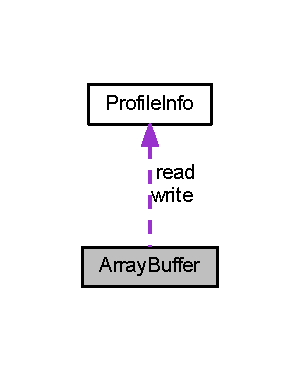
\includegraphics[width=144pt]{class_array_buffer__coll__graph}
\end{center}
\end{figure}
\subsection*{Public Member Functions}
\begin{DoxyCompactItemize}
\item 
\hyperlink{class_array_buffer_a63fcf9bffe928ffa800313815019ac79}{Array\-Buffer} ()
\item 
void \hyperlink{class_array_buffer_a76231eefe415da5bba1754f3cc2045f9}{unpin\-Abort} (J\-N\-I\-Env $\ast$\hyperlink{aparapi_8cpp_a31595c73e9a3750524b2ff61b5a14f96}{jenv})
\item 
void \hyperlink{class_array_buffer_a112827b6241d6f9029e993e4ab419bd2}{unpin\-Commit} (J\-N\-I\-Env $\ast$\hyperlink{aparapi_8cpp_a31595c73e9a3750524b2ff61b5a14f96}{jenv})
\item 
void \hyperlink{class_array_buffer_ae3247a8375aadcdd840780275305c60f}{pin} (J\-N\-I\-Env $\ast$\hyperlink{aparapi_8cpp_a31595c73e9a3750524b2ff61b5a14f96}{jenv})
\end{DoxyCompactItemize}
\subsection*{Public Attributes}
\begin{DoxyCompactItemize}
\item 
jobject \hyperlink{class_array_buffer_aff59baf34e6b6ee7cdf881425d71e407}{java\-Array}
\item 
cl\-\_\-uint \hyperlink{class_array_buffer_adfbebf14a3938a28732161382f654f20}{length}
\item 
jint \hyperlink{class_array_buffer_a30ebc774107e0aeedcad8228f20cacac}{length\-In\-Bytes}
\item 
cl\-\_\-mem \hyperlink{class_array_buffer_a8ceddaf2157d696a6386c5ad2bff9526}{mem}
\item 
void $\ast$ \hyperlink{class_array_buffer_ab3676dd66e12d778c41a0e6cf551cf2f}{addr}
\item 
cl\-\_\-uint \hyperlink{class_array_buffer_a3780a88f8a8b72c0d2894831daf0f95e}{mem\-Mask}
\item 
jboolean \hyperlink{class_array_buffer_a4a1262a3549dfe5e0fe59eebe87d9325}{is\-Copy}
\item 
jboolean \hyperlink{class_array_buffer_a9c367c924157552a61d07c919e2f8c44}{is\-Pinned}
\item 
char \hyperlink{class_array_buffer_ab7228af63eb8955afa0848f05154f964}{mem\-Spec} \mbox{[}128\mbox{]}
\item 
\hyperlink{class_profile_info}{Profile\-Info} \hyperlink{class_array_buffer_a61c626d6492770cc661f3018806cce69}{read}
\item 
\hyperlink{class_profile_info}{Profile\-Info} \hyperlink{class_array_buffer_acbada5a527a38d5d6bd9da4e6f12f556}{write}
\end{DoxyCompactItemize}


\subsection{Constructor \& Destructor Documentation}
\hypertarget{class_array_buffer_a63fcf9bffe928ffa800313815019ac79}{\index{Array\-Buffer@{Array\-Buffer}!Array\-Buffer@{Array\-Buffer}}
\index{Array\-Buffer@{Array\-Buffer}!ArrayBuffer@{Array\-Buffer}}
\subsubsection[{Array\-Buffer}]{\setlength{\rightskip}{0pt plus 5cm}Array\-Buffer\-::\-Array\-Buffer (
\begin{DoxyParamCaption}
{}
\end{DoxyParamCaption}
)}}\label{class_array_buffer_a63fcf9bffe928ffa800313815019ac79}


\subsection{Member Function Documentation}
\hypertarget{class_array_buffer_ae3247a8375aadcdd840780275305c60f}{\index{Array\-Buffer@{Array\-Buffer}!pin@{pin}}
\index{pin@{pin}!ArrayBuffer@{Array\-Buffer}}
\subsubsection[{pin}]{\setlength{\rightskip}{0pt plus 5cm}void Array\-Buffer\-::pin (
\begin{DoxyParamCaption}
\item[{J\-N\-I\-Env $\ast$}]{jenv}
\end{DoxyParamCaption}
)}}\label{class_array_buffer_ae3247a8375aadcdd840780275305c60f}


Here is the caller graph for this function\-:
\nopagebreak
\begin{figure}[H]
\begin{center}
\leavevmode
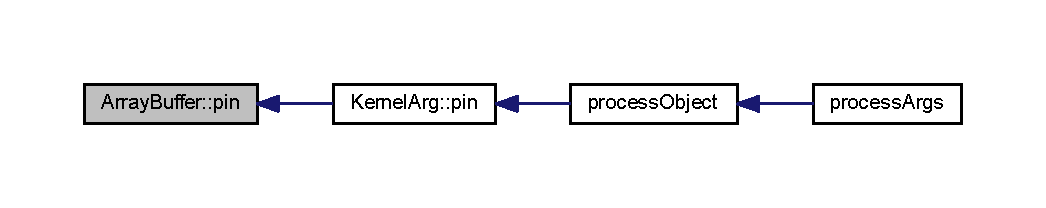
\includegraphics[width=350pt]{class_array_buffer_ae3247a8375aadcdd840780275305c60f_icgraph}
\end{center}
\end{figure}


\hypertarget{class_array_buffer_a76231eefe415da5bba1754f3cc2045f9}{\index{Array\-Buffer@{Array\-Buffer}!unpin\-Abort@{unpin\-Abort}}
\index{unpin\-Abort@{unpin\-Abort}!ArrayBuffer@{Array\-Buffer}}
\subsubsection[{unpin\-Abort}]{\setlength{\rightskip}{0pt plus 5cm}void Array\-Buffer\-::unpin\-Abort (
\begin{DoxyParamCaption}
\item[{J\-N\-I\-Env $\ast$}]{jenv}
\end{DoxyParamCaption}
)}}\label{class_array_buffer_a76231eefe415da5bba1754f3cc2045f9}


Here is the caller graph for this function\-:
\nopagebreak
\begin{figure}[H]
\begin{center}
\leavevmode
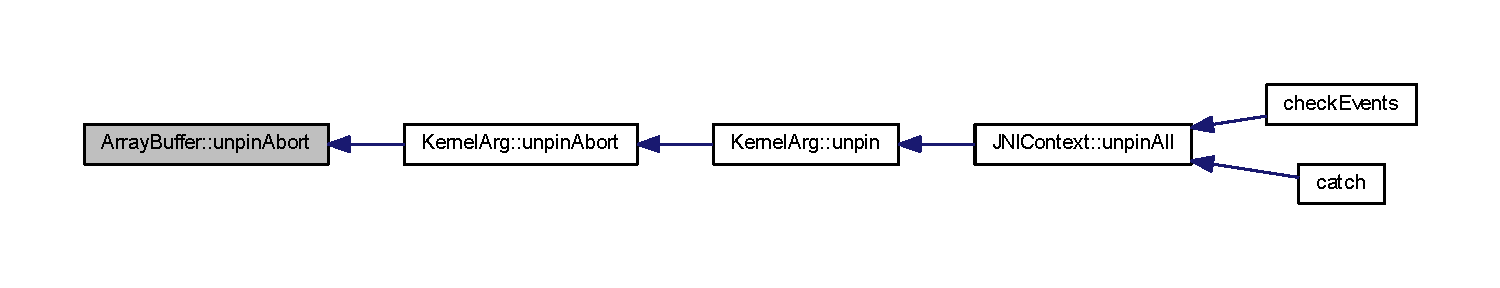
\includegraphics[width=350pt]{class_array_buffer_a76231eefe415da5bba1754f3cc2045f9_icgraph}
\end{center}
\end{figure}


\hypertarget{class_array_buffer_a112827b6241d6f9029e993e4ab419bd2}{\index{Array\-Buffer@{Array\-Buffer}!unpin\-Commit@{unpin\-Commit}}
\index{unpin\-Commit@{unpin\-Commit}!ArrayBuffer@{Array\-Buffer}}
\subsubsection[{unpin\-Commit}]{\setlength{\rightskip}{0pt plus 5cm}void Array\-Buffer\-::unpin\-Commit (
\begin{DoxyParamCaption}
\item[{J\-N\-I\-Env $\ast$}]{jenv}
\end{DoxyParamCaption}
)}}\label{class_array_buffer_a112827b6241d6f9029e993e4ab419bd2}


Here is the caller graph for this function\-:
\nopagebreak
\begin{figure}[H]
\begin{center}
\leavevmode
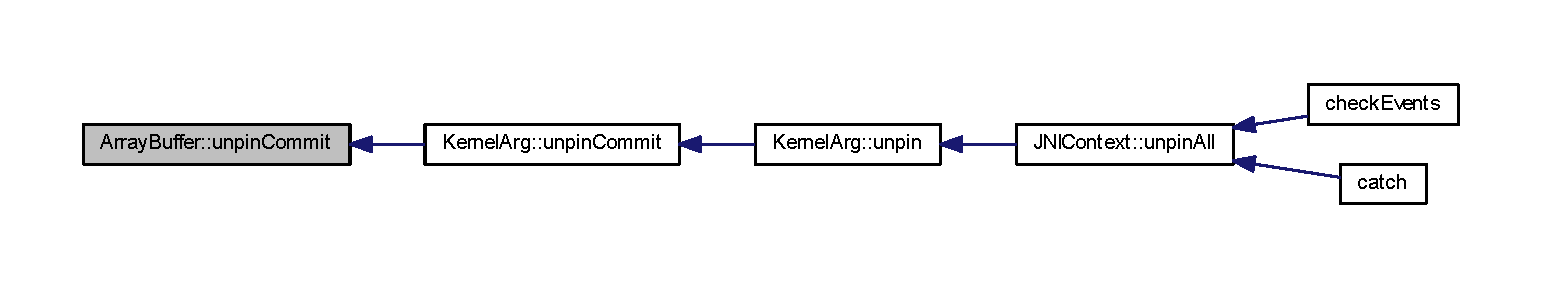
\includegraphics[width=350pt]{class_array_buffer_a112827b6241d6f9029e993e4ab419bd2_icgraph}
\end{center}
\end{figure}




\subsection{Member Data Documentation}
\hypertarget{class_array_buffer_ab3676dd66e12d778c41a0e6cf551cf2f}{\index{Array\-Buffer@{Array\-Buffer}!addr@{addr}}
\index{addr@{addr}!ArrayBuffer@{Array\-Buffer}}
\subsubsection[{addr}]{\setlength{\rightskip}{0pt plus 5cm}void$\ast$ Array\-Buffer\-::addr}}\label{class_array_buffer_ab3676dd66e12d778c41a0e6cf551cf2f}
\hypertarget{class_array_buffer_a4a1262a3549dfe5e0fe59eebe87d9325}{\index{Array\-Buffer@{Array\-Buffer}!is\-Copy@{is\-Copy}}
\index{is\-Copy@{is\-Copy}!ArrayBuffer@{Array\-Buffer}}
\subsubsection[{is\-Copy}]{\setlength{\rightskip}{0pt plus 5cm}jboolean Array\-Buffer\-::is\-Copy}}\label{class_array_buffer_a4a1262a3549dfe5e0fe59eebe87d9325}
\hypertarget{class_array_buffer_a9c367c924157552a61d07c919e2f8c44}{\index{Array\-Buffer@{Array\-Buffer}!is\-Pinned@{is\-Pinned}}
\index{is\-Pinned@{is\-Pinned}!ArrayBuffer@{Array\-Buffer}}
\subsubsection[{is\-Pinned}]{\setlength{\rightskip}{0pt plus 5cm}jboolean Array\-Buffer\-::is\-Pinned}}\label{class_array_buffer_a9c367c924157552a61d07c919e2f8c44}
\hypertarget{class_array_buffer_aff59baf34e6b6ee7cdf881425d71e407}{\index{Array\-Buffer@{Array\-Buffer}!java\-Array@{java\-Array}}
\index{java\-Array@{java\-Array}!ArrayBuffer@{Array\-Buffer}}
\subsubsection[{java\-Array}]{\setlength{\rightskip}{0pt plus 5cm}jobject Array\-Buffer\-::java\-Array}}\label{class_array_buffer_aff59baf34e6b6ee7cdf881425d71e407}
\hypertarget{class_array_buffer_adfbebf14a3938a28732161382f654f20}{\index{Array\-Buffer@{Array\-Buffer}!length@{length}}
\index{length@{length}!ArrayBuffer@{Array\-Buffer}}
\subsubsection[{length}]{\setlength{\rightskip}{0pt plus 5cm}cl\-\_\-uint Array\-Buffer\-::length}}\label{class_array_buffer_adfbebf14a3938a28732161382f654f20}
\hypertarget{class_array_buffer_a30ebc774107e0aeedcad8228f20cacac}{\index{Array\-Buffer@{Array\-Buffer}!length\-In\-Bytes@{length\-In\-Bytes}}
\index{length\-In\-Bytes@{length\-In\-Bytes}!ArrayBuffer@{Array\-Buffer}}
\subsubsection[{length\-In\-Bytes}]{\setlength{\rightskip}{0pt plus 5cm}jint Array\-Buffer\-::length\-In\-Bytes}}\label{class_array_buffer_a30ebc774107e0aeedcad8228f20cacac}
\hypertarget{class_array_buffer_a8ceddaf2157d696a6386c5ad2bff9526}{\index{Array\-Buffer@{Array\-Buffer}!mem@{mem}}
\index{mem@{mem}!ArrayBuffer@{Array\-Buffer}}
\subsubsection[{mem}]{\setlength{\rightskip}{0pt plus 5cm}cl\-\_\-mem Array\-Buffer\-::mem}}\label{class_array_buffer_a8ceddaf2157d696a6386c5ad2bff9526}
\hypertarget{class_array_buffer_a3780a88f8a8b72c0d2894831daf0f95e}{\index{Array\-Buffer@{Array\-Buffer}!mem\-Mask@{mem\-Mask}}
\index{mem\-Mask@{mem\-Mask}!ArrayBuffer@{Array\-Buffer}}
\subsubsection[{mem\-Mask}]{\setlength{\rightskip}{0pt plus 5cm}cl\-\_\-uint Array\-Buffer\-::mem\-Mask}}\label{class_array_buffer_a3780a88f8a8b72c0d2894831daf0f95e}
\hypertarget{class_array_buffer_ab7228af63eb8955afa0848f05154f964}{\index{Array\-Buffer@{Array\-Buffer}!mem\-Spec@{mem\-Spec}}
\index{mem\-Spec@{mem\-Spec}!ArrayBuffer@{Array\-Buffer}}
\subsubsection[{mem\-Spec}]{\setlength{\rightskip}{0pt plus 5cm}char Array\-Buffer\-::mem\-Spec\mbox{[}128\mbox{]}}}\label{class_array_buffer_ab7228af63eb8955afa0848f05154f964}
\hypertarget{class_array_buffer_a61c626d6492770cc661f3018806cce69}{\index{Array\-Buffer@{Array\-Buffer}!read@{read}}
\index{read@{read}!ArrayBuffer@{Array\-Buffer}}
\subsubsection[{read}]{\setlength{\rightskip}{0pt plus 5cm}{\bf Profile\-Info} Array\-Buffer\-::read}}\label{class_array_buffer_a61c626d6492770cc661f3018806cce69}
\hypertarget{class_array_buffer_acbada5a527a38d5d6bd9da4e6f12f556}{\index{Array\-Buffer@{Array\-Buffer}!write@{write}}
\index{write@{write}!ArrayBuffer@{Array\-Buffer}}
\subsubsection[{write}]{\setlength{\rightskip}{0pt plus 5cm}{\bf Profile\-Info} Array\-Buffer\-::write}}\label{class_array_buffer_acbada5a527a38d5d6bd9da4e6f12f556}


The documentation for this class was generated from the following files\-:\begin{DoxyCompactItemize}
\item 
src/cpp/run\-Kernel/\hyperlink{array_buffer_8h}{array\-Buffer.\-h}\item 
src/cpp/run\-Kernel/\hyperlink{array_buffer_8cpp}{array\-Buffer.\-cpp}\end{DoxyCompactItemize}

\hypertarget{class_c_l_exception}{\section{C\-L\-Exception Class Reference}
\label{class_c_l_exception}\index{C\-L\-Exception@{C\-L\-Exception}}
}


{\ttfamily \#include $<$C\-L\-Exception.\-h$>$}



Inheritance diagram for C\-L\-Exception\-:
\nopagebreak
\begin{figure}[H]
\begin{center}
\leavevmode
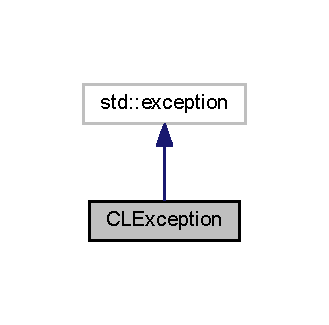
\includegraphics[width=158pt]{class_c_l_exception__inherit__graph}
\end{center}
\end{figure}


Collaboration diagram for C\-L\-Exception\-:
\nopagebreak
\begin{figure}[H]
\begin{center}
\leavevmode
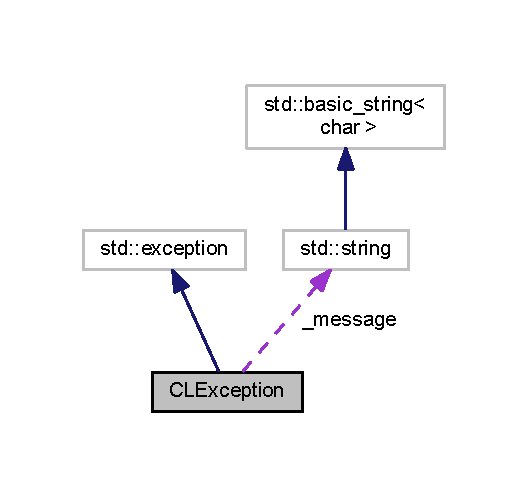
\includegraphics[width=253pt]{class_c_l_exception__coll__graph}
\end{center}
\end{figure}
\subsection*{Public Member Functions}
\begin{DoxyCompactItemize}
\item 
\hyperlink{class_c_l_exception_a22033255f193444c7038dd3ed1314c3e}{$\sim$\-C\-L\-Exception} ()  throw ()
\item 
\hyperlink{class_c_l_exception_a24089a34df64c03ae5b90818dd8598ec}{C\-L\-Exception} (int \hyperlink{class_c_l_exception_a08feb7c76971320d736c4137a03013bb}{status}, std\-::string \hyperlink{class_c_l_exception_afaeb1a33cb858c0faa74fa6538a97dc5}{message})
\item 
\hyperlink{class_c_l_exception_a89c27aa8b28775ffd8e52c708bcc6fa0}{C\-L\-Exception} (const \hyperlink{class_c_l_exception}{C\-L\-Exception} \&cle)
\item 
\hyperlink{class_c_l_exception}{C\-L\-Exception} \& \hyperlink{class_c_l_exception_a735f300c25668ba7c00e1a83c0c0dca3}{operator=} (const \hyperlink{class_c_l_exception}{C\-L\-Exception} \&cle)
\item 
int \hyperlink{class_c_l_exception_a08feb7c76971320d736c4137a03013bb}{status} ()
\item 
const char $\ast$ \hyperlink{class_c_l_exception_afaeb1a33cb858c0faa74fa6538a97dc5}{message} ()
\item 
void \hyperlink{class_c_l_exception_a0c1d6917db38876465e60f1404e589d3}{print\-Error} ()
\item 
const char $\ast$ \hyperlink{class_c_l_exception_a8275eb0a5a0ac4ab0de4bad4b0130d0e}{what} ()
\end{DoxyCompactItemize}
\subsection*{Static Public Member Functions}
\begin{DoxyCompactItemize}
\item 
static void \hyperlink{class_c_l_exception_a499ceca093813dcd2e731f542b1e078e}{check\-C\-L\-Error} (cl\-\_\-int \hyperlink{class_c_l_exception_a08feb7c76971320d736c4137a03013bb}{status}, std\-::string error)
\end{DoxyCompactItemize}
\subsection*{Private Attributes}
\begin{DoxyCompactItemize}
\item 
int \hyperlink{class_c_l_exception_aa8b72fb16bc1bbd38c28bc2bbc4fee28}{\-\_\-status}
\item 
std\-::string \hyperlink{class_c_l_exception_a05349664de93edb8e6379f67fe63a9e2}{\-\_\-message}
\end{DoxyCompactItemize}


\subsection{Constructor \& Destructor Documentation}
\hypertarget{class_c_l_exception_a22033255f193444c7038dd3ed1314c3e}{\index{C\-L\-Exception@{C\-L\-Exception}!$\sim$\-C\-L\-Exception@{$\sim$\-C\-L\-Exception}}
\index{$\sim$\-C\-L\-Exception@{$\sim$\-C\-L\-Exception}!CLException@{C\-L\-Exception}}
\subsubsection[{$\sim$\-C\-L\-Exception}]{\setlength{\rightskip}{0pt plus 5cm}C\-L\-Exception\-::$\sim$\-C\-L\-Exception (
\begin{DoxyParamCaption}
{}
\end{DoxyParamCaption}
)  throw ()\hspace{0.3cm}{\ttfamily [inline]}}}\label{class_c_l_exception_a22033255f193444c7038dd3ed1314c3e}
\hypertarget{class_c_l_exception_a24089a34df64c03ae5b90818dd8598ec}{\index{C\-L\-Exception@{C\-L\-Exception}!C\-L\-Exception@{C\-L\-Exception}}
\index{C\-L\-Exception@{C\-L\-Exception}!CLException@{C\-L\-Exception}}
\subsubsection[{C\-L\-Exception}]{\setlength{\rightskip}{0pt plus 5cm}C\-L\-Exception\-::\-C\-L\-Exception (
\begin{DoxyParamCaption}
\item[{int}]{status, }
\item[{std\-::string}]{message}
\end{DoxyParamCaption}
)\hspace{0.3cm}{\ttfamily [inline]}}}\label{class_c_l_exception_a24089a34df64c03ae5b90818dd8598ec}


Here is the call graph for this function\-:
\nopagebreak
\begin{figure}[H]
\begin{center}
\leavevmode
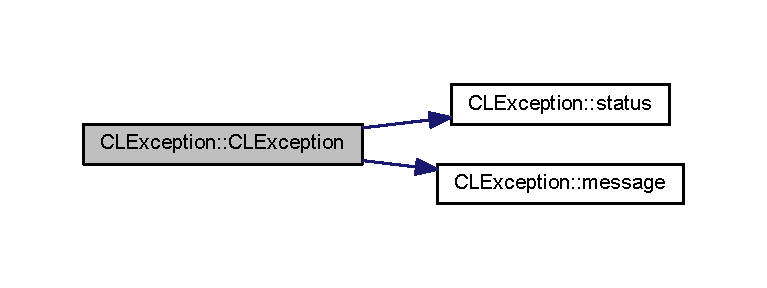
\includegraphics[width=350pt]{class_c_l_exception_a24089a34df64c03ae5b90818dd8598ec_cgraph}
\end{center}
\end{figure}




Here is the caller graph for this function\-:
\nopagebreak
\begin{figure}[H]
\begin{center}
\leavevmode
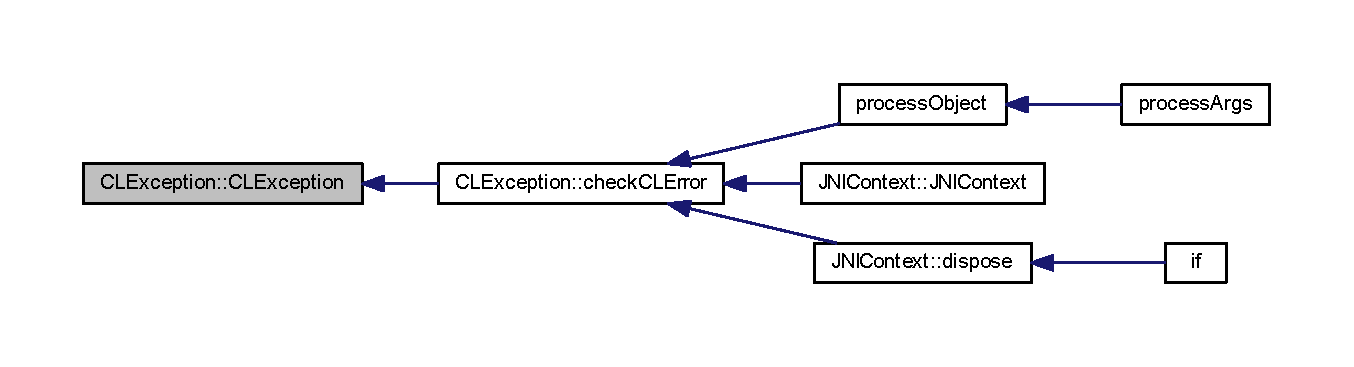
\includegraphics[width=350pt]{class_c_l_exception_a24089a34df64c03ae5b90818dd8598ec_icgraph}
\end{center}
\end{figure}


\hypertarget{class_c_l_exception_a89c27aa8b28775ffd8e52c708bcc6fa0}{\index{C\-L\-Exception@{C\-L\-Exception}!C\-L\-Exception@{C\-L\-Exception}}
\index{C\-L\-Exception@{C\-L\-Exception}!CLException@{C\-L\-Exception}}
\subsubsection[{C\-L\-Exception}]{\setlength{\rightskip}{0pt plus 5cm}C\-L\-Exception\-::\-C\-L\-Exception (
\begin{DoxyParamCaption}
\item[{const {\bf C\-L\-Exception} \&}]{cle}
\end{DoxyParamCaption}
)\hspace{0.3cm}{\ttfamily [inline]}}}\label{class_c_l_exception_a89c27aa8b28775ffd8e52c708bcc6fa0}


\subsection{Member Function Documentation}
\hypertarget{class_c_l_exception_a499ceca093813dcd2e731f542b1e078e}{\index{C\-L\-Exception@{C\-L\-Exception}!check\-C\-L\-Error@{check\-C\-L\-Error}}
\index{check\-C\-L\-Error@{check\-C\-L\-Error}!CLException@{C\-L\-Exception}}
\subsubsection[{check\-C\-L\-Error}]{\setlength{\rightskip}{0pt plus 5cm}static void C\-L\-Exception\-::check\-C\-L\-Error (
\begin{DoxyParamCaption}
\item[{cl\-\_\-int}]{status, }
\item[{std\-::string}]{error}
\end{DoxyParamCaption}
)\hspace{0.3cm}{\ttfamily [inline]}, {\ttfamily [static]}}}\label{class_c_l_exception_a499ceca093813dcd2e731f542b1e078e}


Here is the call graph for this function\-:
\nopagebreak
\begin{figure}[H]
\begin{center}
\leavevmode
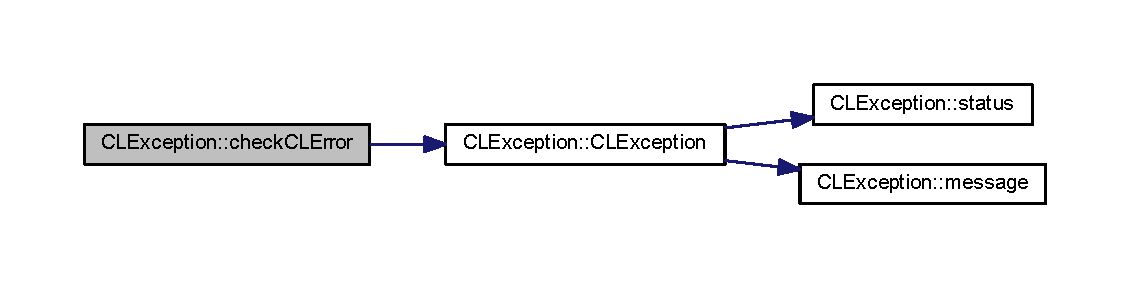
\includegraphics[width=350pt]{class_c_l_exception_a499ceca093813dcd2e731f542b1e078e_cgraph}
\end{center}
\end{figure}




Here is the caller graph for this function\-:
\nopagebreak
\begin{figure}[H]
\begin{center}
\leavevmode
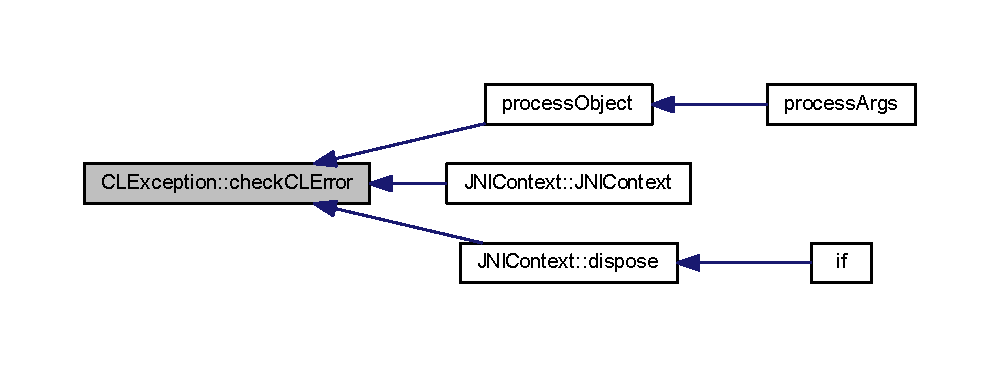
\includegraphics[width=350pt]{class_c_l_exception_a499ceca093813dcd2e731f542b1e078e_icgraph}
\end{center}
\end{figure}


\hypertarget{class_c_l_exception_afaeb1a33cb858c0faa74fa6538a97dc5}{\index{C\-L\-Exception@{C\-L\-Exception}!message@{message}}
\index{message@{message}!CLException@{C\-L\-Exception}}
\subsubsection[{message}]{\setlength{\rightskip}{0pt plus 5cm}const char$\ast$ C\-L\-Exception\-::message (
\begin{DoxyParamCaption}
{}
\end{DoxyParamCaption}
)\hspace{0.3cm}{\ttfamily [inline]}}}\label{class_c_l_exception_afaeb1a33cb858c0faa74fa6538a97dc5}


Here is the caller graph for this function\-:
\nopagebreak
\begin{figure}[H]
\begin{center}
\leavevmode
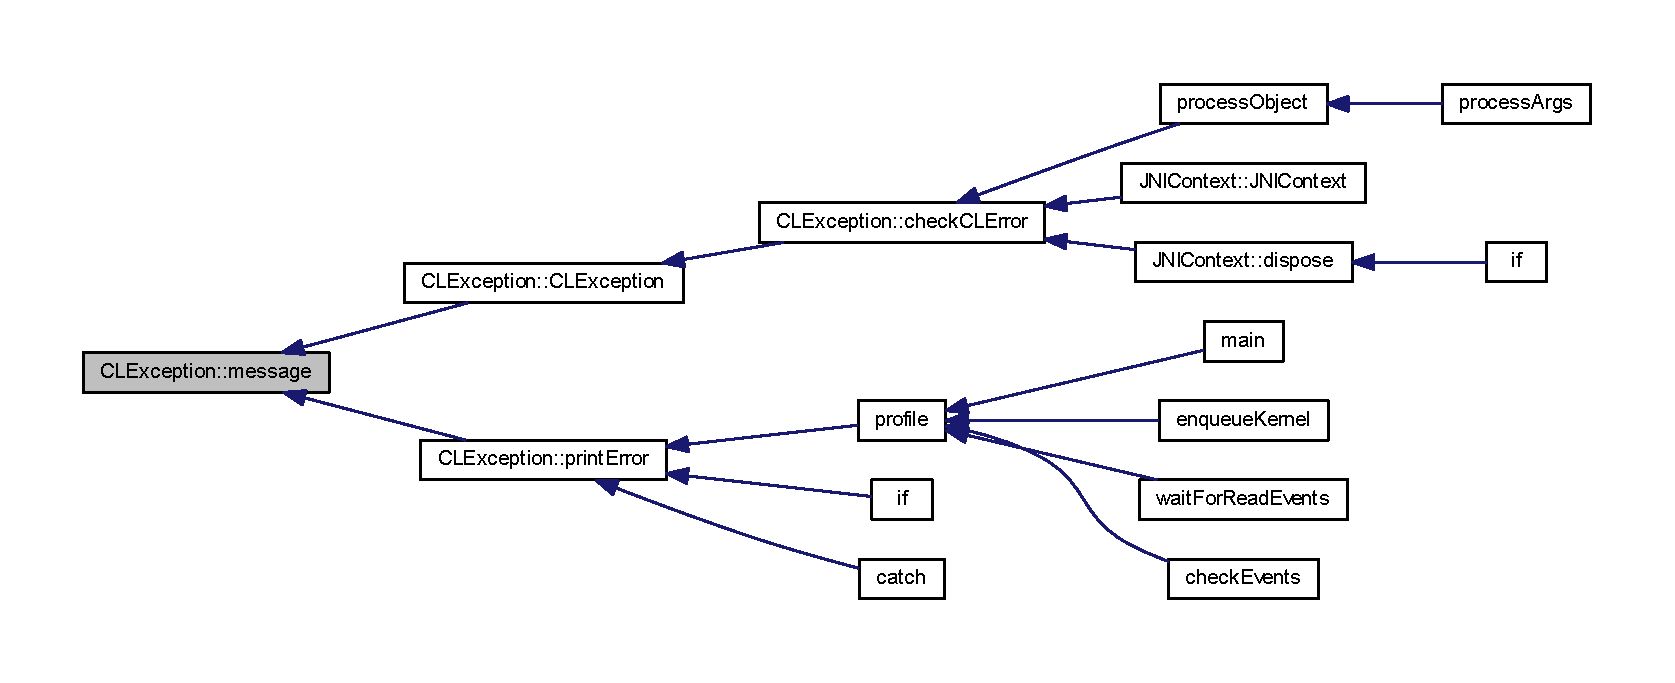
\includegraphics[width=350pt]{class_c_l_exception_afaeb1a33cb858c0faa74fa6538a97dc5_icgraph}
\end{center}
\end{figure}


\hypertarget{class_c_l_exception_a735f300c25668ba7c00e1a83c0c0dca3}{\index{C\-L\-Exception@{C\-L\-Exception}!operator=@{operator=}}
\index{operator=@{operator=}!CLException@{C\-L\-Exception}}
\subsubsection[{operator=}]{\setlength{\rightskip}{0pt plus 5cm}{\bf C\-L\-Exception}\& C\-L\-Exception\-::operator= (
\begin{DoxyParamCaption}
\item[{const {\bf C\-L\-Exception} \&}]{cle}
\end{DoxyParamCaption}
)\hspace{0.3cm}{\ttfamily [inline]}}}\label{class_c_l_exception_a735f300c25668ba7c00e1a83c0c0dca3}
\hypertarget{class_c_l_exception_a0c1d6917db38876465e60f1404e589d3}{\index{C\-L\-Exception@{C\-L\-Exception}!print\-Error@{print\-Error}}
\index{print\-Error@{print\-Error}!CLException@{C\-L\-Exception}}
\subsubsection[{print\-Error}]{\setlength{\rightskip}{0pt plus 5cm}void C\-L\-Exception\-::print\-Error (
\begin{DoxyParamCaption}
{}
\end{DoxyParamCaption}
)\hspace{0.3cm}{\ttfamily [inline]}}}\label{class_c_l_exception_a0c1d6917db38876465e60f1404e589d3}


Here is the call graph for this function\-:
\nopagebreak
\begin{figure}[H]
\begin{center}
\leavevmode
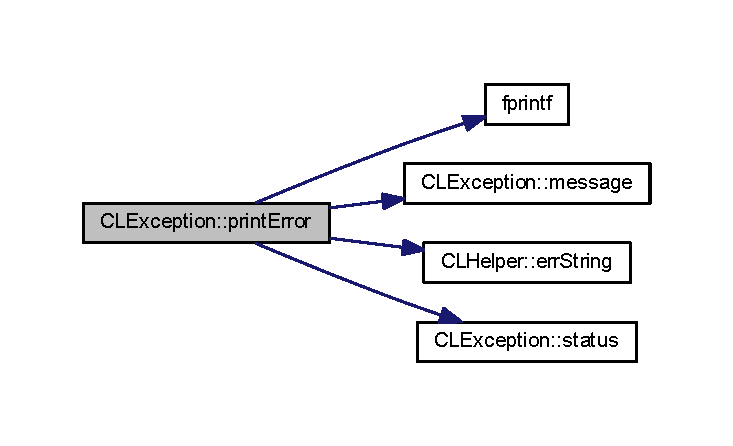
\includegraphics[width=350pt]{class_c_l_exception_a0c1d6917db38876465e60f1404e589d3_cgraph}
\end{center}
\end{figure}




Here is the caller graph for this function\-:
\nopagebreak
\begin{figure}[H]
\begin{center}
\leavevmode
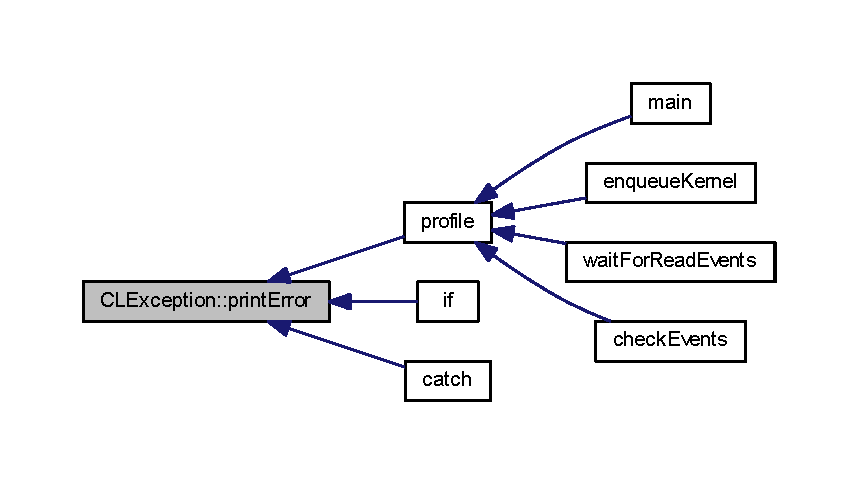
\includegraphics[width=350pt]{class_c_l_exception_a0c1d6917db38876465e60f1404e589d3_icgraph}
\end{center}
\end{figure}


\hypertarget{class_c_l_exception_a08feb7c76971320d736c4137a03013bb}{\index{C\-L\-Exception@{C\-L\-Exception}!status@{status}}
\index{status@{status}!CLException@{C\-L\-Exception}}
\subsubsection[{status}]{\setlength{\rightskip}{0pt plus 5cm}int C\-L\-Exception\-::status (
\begin{DoxyParamCaption}
{}
\end{DoxyParamCaption}
)\hspace{0.3cm}{\ttfamily [inline]}}}\label{class_c_l_exception_a08feb7c76971320d736c4137a03013bb}


Here is the caller graph for this function\-:
\nopagebreak
\begin{figure}[H]
\begin{center}
\leavevmode
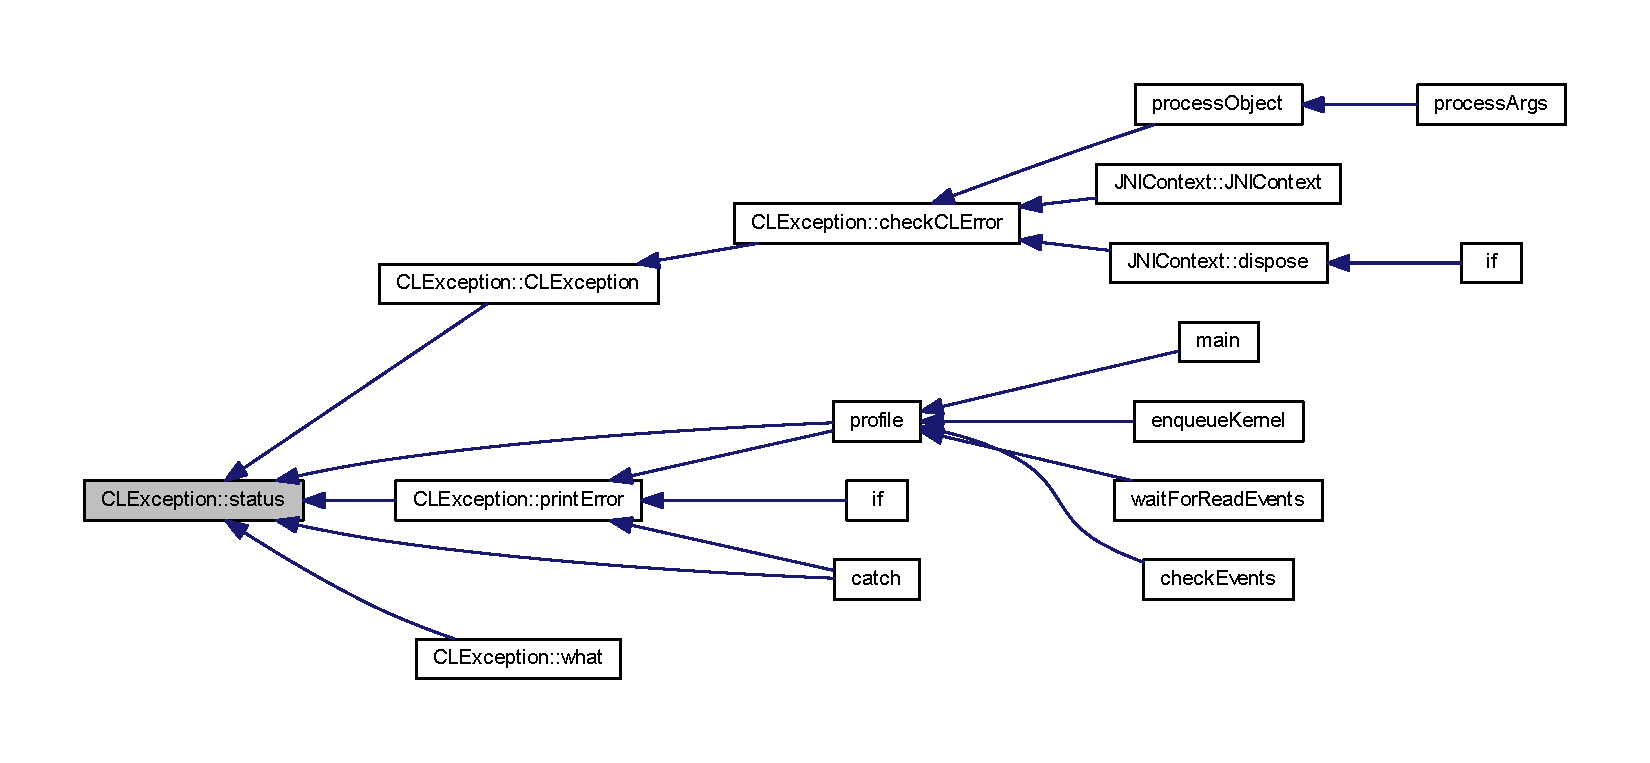
\includegraphics[width=350pt]{class_c_l_exception_a08feb7c76971320d736c4137a03013bb_icgraph}
\end{center}
\end{figure}


\hypertarget{class_c_l_exception_a8275eb0a5a0ac4ab0de4bad4b0130d0e}{\index{C\-L\-Exception@{C\-L\-Exception}!what@{what}}
\index{what@{what}!CLException@{C\-L\-Exception}}
\subsubsection[{what}]{\setlength{\rightskip}{0pt plus 5cm}const char$\ast$ C\-L\-Exception\-::what (
\begin{DoxyParamCaption}
{}
\end{DoxyParamCaption}
)\hspace{0.3cm}{\ttfamily [inline]}}}\label{class_c_l_exception_a8275eb0a5a0ac4ab0de4bad4b0130d0e}


Here is the call graph for this function\-:
\nopagebreak
\begin{figure}[H]
\begin{center}
\leavevmode
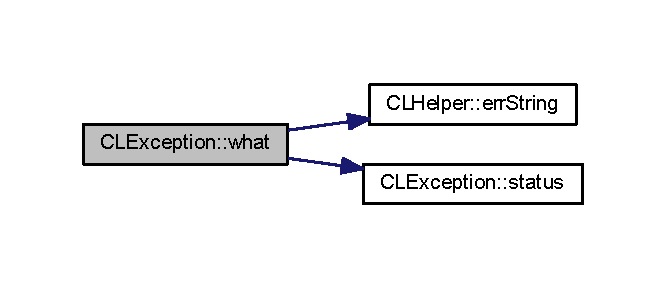
\includegraphics[width=320pt]{class_c_l_exception_a8275eb0a5a0ac4ab0de4bad4b0130d0e_cgraph}
\end{center}
\end{figure}




\subsection{Member Data Documentation}
\hypertarget{class_c_l_exception_a05349664de93edb8e6379f67fe63a9e2}{\index{C\-L\-Exception@{C\-L\-Exception}!\-\_\-message@{\-\_\-message}}
\index{\-\_\-message@{\-\_\-message}!CLException@{C\-L\-Exception}}
\subsubsection[{\-\_\-message}]{\setlength{\rightskip}{0pt plus 5cm}std\-::string C\-L\-Exception\-::\-\_\-message\hspace{0.3cm}{\ttfamily [private]}}}\label{class_c_l_exception_a05349664de93edb8e6379f67fe63a9e2}
\hypertarget{class_c_l_exception_aa8b72fb16bc1bbd38c28bc2bbc4fee28}{\index{C\-L\-Exception@{C\-L\-Exception}!\-\_\-status@{\-\_\-status}}
\index{\-\_\-status@{\-\_\-status}!CLException@{C\-L\-Exception}}
\subsubsection[{\-\_\-status}]{\setlength{\rightskip}{0pt plus 5cm}int C\-L\-Exception\-::\-\_\-status\hspace{0.3cm}{\ttfamily [private]}}}\label{class_c_l_exception_aa8b72fb16bc1bbd38c28bc2bbc4fee28}


The documentation for this class was generated from the following file\-:\begin{DoxyCompactItemize}
\item 
src/cpp/\hyperlink{_c_l_exception_8h}{C\-L\-Exception.\-h}\end{DoxyCompactItemize}

\hypertarget{class_c_l_helper}{\section{C\-L\-Helper Class Reference}
\label{class_c_l_helper}\index{C\-L\-Helper@{C\-L\-Helper}}
}


{\ttfamily \#include $<$cl\-Helper.\-h$>$}

\subsection*{Static Public Member Functions}
\begin{DoxyCompactItemize}
\item 
static const char $\ast$ \hyperlink{class_c_l_helper_acdb10aebef4162371ac53e6fb6835c67}{err\-String} (cl\-\_\-int \hyperlink{aparapi_8cpp_a8d29973874cd2ac670823237b281069e}{status})
\item 
static void \hyperlink{class_c_l_helper_a701cbf42de8d2a5426cbee1d022f74ac}{get\-Build\-Err} (J\-N\-I\-Env $\ast$\hyperlink{aparapi_8cpp_a31595c73e9a3750524b2ff61b5a14f96}{jenv}, cl\-\_\-device\-\_\-id \hyperlink{opencljni_8cpp_aee8691126c8634ec30bfe4f704b3fd7a}{device\-Id}, cl\-\_\-program \hyperlink{aparapi_8cpp_ac70709e80332d58701f9623a803c8541}{program}, jstring $\ast$log)
\item 
static cl\-\_\-program \hyperlink{class_c_l_helper_a14600eb913779f2122461e3293c600dd}{compile} (J\-N\-I\-Env $\ast$\hyperlink{aparapi_8cpp_a31595c73e9a3750524b2ff61b5a14f96}{jenv}, cl\-\_\-context context, size\-\_\-t device\-Count, cl\-\_\-device\-\_\-id $\ast$\hyperlink{opencljni_8cpp_aee8691126c8634ec30bfe4f704b3fd7a}{device\-Id}, jstring \hyperlink{aparapi_8cpp_ab6f02de0fea282662dc1f6ac445ec5f3}{source}, jstring $\ast$log, cl\-\_\-int $\ast$\hyperlink{aparapi_8cpp_a8d29973874cd2ac670823237b281069e}{status})
\item 
static jstring \hyperlink{class_c_l_helper_a76a419374af4d200ee68c537d7c882e5}{get\-Extensions} (J\-N\-I\-Env $\ast$\hyperlink{aparapi_8cpp_a31595c73e9a3750524b2ff61b5a14f96}{jenv}, cl\-\_\-device\-\_\-id \hyperlink{opencljni_8cpp_aee8691126c8634ec30bfe4f704b3fd7a}{device\-Id}, cl\-\_\-int $\ast$\hyperlink{aparapi_8cpp_a8d29973874cd2ac670823237b281069e}{status})
\end{DoxyCompactItemize}


\subsection{Member Function Documentation}
\hypertarget{class_c_l_helper_a14600eb913779f2122461e3293c600dd}{\index{C\-L\-Helper@{C\-L\-Helper}!compile@{compile}}
\index{compile@{compile}!CLHelper@{C\-L\-Helper}}
\subsubsection[{compile}]{\setlength{\rightskip}{0pt plus 5cm}cl\-\_\-program C\-L\-Helper\-::compile (
\begin{DoxyParamCaption}
\item[{J\-N\-I\-Env $\ast$}]{jenv, }
\item[{cl\-\_\-context}]{context, }
\item[{size\-\_\-t}]{device\-Count, }
\item[{cl\-\_\-device\-\_\-id $\ast$}]{device\-Id, }
\item[{jstring}]{source, }
\item[{jstring $\ast$}]{log, }
\item[{cl\-\_\-int $\ast$}]{status}
\end{DoxyParamCaption}
)\hspace{0.3cm}{\ttfamily [static]}}}\label{class_c_l_helper_a14600eb913779f2122461e3293c600dd}


Here is the call graph for this function\-:
\nopagebreak
\begin{figure}[H]
\begin{center}
\leavevmode
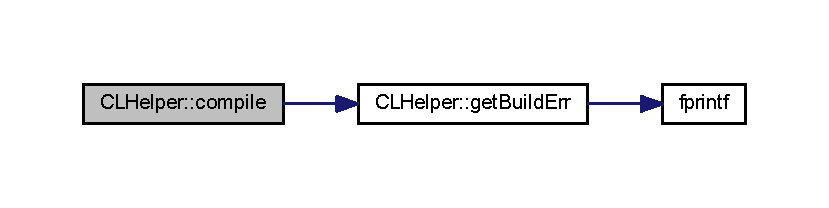
\includegraphics[width=350pt]{class_c_l_helper_a14600eb913779f2122461e3293c600dd_cgraph}
\end{center}
\end{figure}


\hypertarget{class_c_l_helper_acdb10aebef4162371ac53e6fb6835c67}{\index{C\-L\-Helper@{C\-L\-Helper}!err\-String@{err\-String}}
\index{err\-String@{err\-String}!CLHelper@{C\-L\-Helper}}
\subsubsection[{err\-String}]{\setlength{\rightskip}{0pt plus 5cm}const char $\ast$ C\-L\-Helper\-::err\-String (
\begin{DoxyParamCaption}
\item[{cl\-\_\-int}]{status}
\end{DoxyParamCaption}
)\hspace{0.3cm}{\ttfamily [static]}}}\label{class_c_l_helper_acdb10aebef4162371ac53e6fb6835c67}


Here is the caller graph for this function\-:
\nopagebreak
\begin{figure}[H]
\begin{center}
\leavevmode
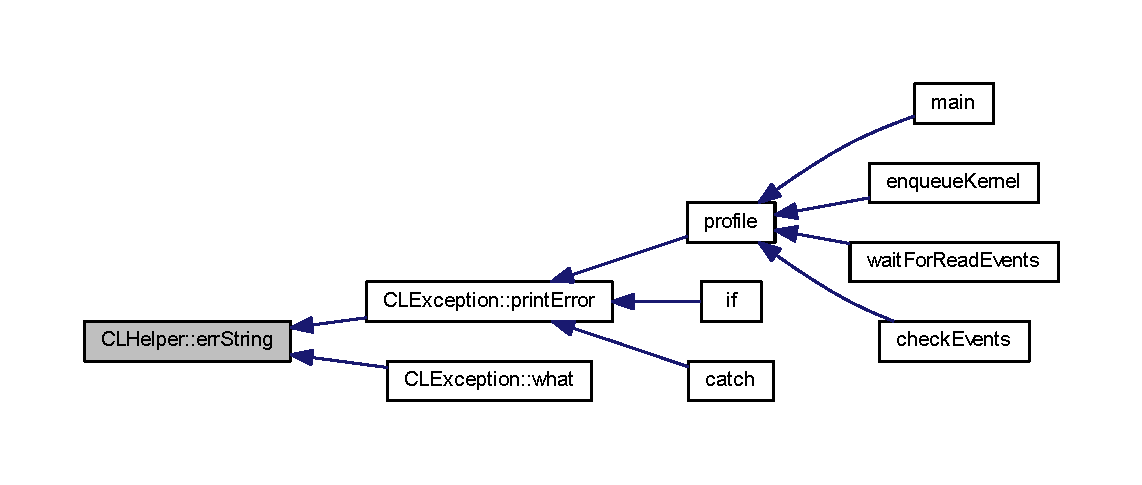
\includegraphics[width=350pt]{class_c_l_helper_acdb10aebef4162371ac53e6fb6835c67_icgraph}
\end{center}
\end{figure}


\hypertarget{class_c_l_helper_a701cbf42de8d2a5426cbee1d022f74ac}{\index{C\-L\-Helper@{C\-L\-Helper}!get\-Build\-Err@{get\-Build\-Err}}
\index{get\-Build\-Err@{get\-Build\-Err}!CLHelper@{C\-L\-Helper}}
\subsubsection[{get\-Build\-Err}]{\setlength{\rightskip}{0pt plus 5cm}void C\-L\-Helper\-::get\-Build\-Err (
\begin{DoxyParamCaption}
\item[{J\-N\-I\-Env $\ast$}]{jenv, }
\item[{cl\-\_\-device\-\_\-id}]{device\-Id, }
\item[{cl\-\_\-program}]{program, }
\item[{jstring $\ast$}]{log}
\end{DoxyParamCaption}
)\hspace{0.3cm}{\ttfamily [static]}}}\label{class_c_l_helper_a701cbf42de8d2a5426cbee1d022f74ac}


Here is the call graph for this function\-:
\nopagebreak
\begin{figure}[H]
\begin{center}
\leavevmode
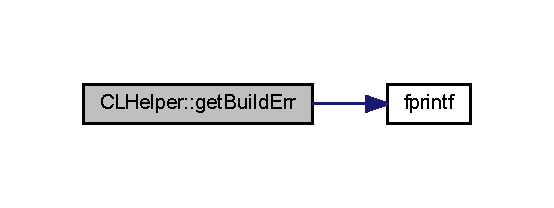
\includegraphics[width=266pt]{class_c_l_helper_a701cbf42de8d2a5426cbee1d022f74ac_cgraph}
\end{center}
\end{figure}




Here is the caller graph for this function\-:
\nopagebreak
\begin{figure}[H]
\begin{center}
\leavevmode
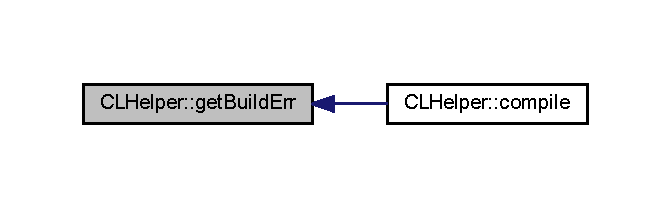
\includegraphics[width=322pt]{class_c_l_helper_a701cbf42de8d2a5426cbee1d022f74ac_icgraph}
\end{center}
\end{figure}


\hypertarget{class_c_l_helper_a76a419374af4d200ee68c537d7c882e5}{\index{C\-L\-Helper@{C\-L\-Helper}!get\-Extensions@{get\-Extensions}}
\index{get\-Extensions@{get\-Extensions}!CLHelper@{C\-L\-Helper}}
\subsubsection[{get\-Extensions}]{\setlength{\rightskip}{0pt plus 5cm}jstring C\-L\-Helper\-::get\-Extensions (
\begin{DoxyParamCaption}
\item[{J\-N\-I\-Env $\ast$}]{jenv, }
\item[{cl\-\_\-device\-\_\-id}]{device\-Id, }
\item[{cl\-\_\-int $\ast$}]{status}
\end{DoxyParamCaption}
)\hspace{0.3cm}{\ttfamily [static]}}}\label{class_c_l_helper_a76a419374af4d200ee68c537d7c882e5}


Here is the call graph for this function\-:
\nopagebreak
\begin{figure}[H]
\begin{center}
\leavevmode
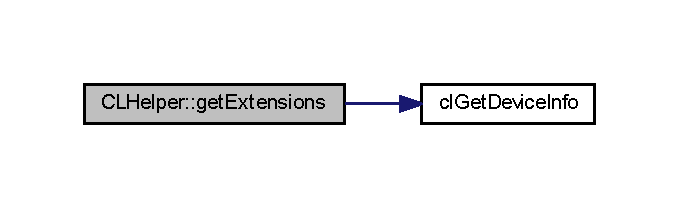
\includegraphics[width=326pt]{class_c_l_helper_a76a419374af4d200ee68c537d7c882e5_cgraph}
\end{center}
\end{figure}




The documentation for this class was generated from the following files\-:\begin{DoxyCompactItemize}
\item 
src/cpp/\hyperlink{cl_helper_8h}{cl\-Helper.\-h}\item 
src/cpp/\hyperlink{cl_helper_8cpp}{cl\-Helper.\-cpp}\end{DoxyCompactItemize}

\hypertarget{class_config}{\section{Config Class Reference}
\label{class_config}\index{Config@{Config}}
}


{\ttfamily \#include $<$config.\-h$>$}

\subsection*{Public Member Functions}
\begin{DoxyCompactItemize}
\item 
jboolean \hyperlink{class_config_a7d99bbf69b5d0632196a2da20294963c}{get\-Boolean} (J\-N\-I\-Env $\ast$\hyperlink{aparapi_8cpp_a31595c73e9a3750524b2ff61b5a14f96}{jenv}, char $\ast$field\-Name)
\item 
\hyperlink{class_config_a15f0fb9274e3f774cb6922e2eecf7208}{Config} (J\-N\-I\-Env $\ast$\hyperlink{aparapi_8cpp_a31595c73e9a3750524b2ff61b5a14f96}{jenv})
\item 
jboolean \hyperlink{class_config_a03234dbe1adbe1c8fdde649df372926c}{is\-Verbose} ()
\item 
jboolean \hyperlink{class_config_a6038fb1fbd5089d24afa3b71fd6c0220}{is\-Profiling\-C\-S\-V\-Enabled} ()
\item 
jboolean \hyperlink{class_config_a7a2cfa5be8d976099dedb684e9c32ca0}{is\-Tracking\-Open\-C\-L\-Resources} ()
\item 
jboolean \hyperlink{class_config_ac91f68d97d5ca75b787d6ea9cba882e4}{is\-Profiling\-Enabled} ()
\end{DoxyCompactItemize}
\subsection*{Public Attributes}
\begin{DoxyCompactItemize}
\item 
jboolean \hyperlink{class_config_a84a74c64a238bf8c965c475de0b17124}{configured}
\item 
jclass \hyperlink{class_config_a7e79ccce393887ace81c263dbc82b0e1}{config\-Class}
\item 
jboolean \hyperlink{class_config_af48b23080ff93b7f7720f228715c4eb2}{enable\-Verbose\-J\-N\-I}
\item 
jboolean \hyperlink{class_config_a40e02509e9330fa8d16087e7dde8a977}{enable\-Verbose\-J\-N\-I\-Open\-C\-L\-Resource\-Tracking}
\item 
jboolean \hyperlink{class_config_a403c9cdc52ef31d933ee055d3165a35e}{enable\-Profiling}
\item 
jboolean \hyperlink{class_config_afb0e37ad017cbf220fcac529fa644944}{enable\-Profiling\-C\-S\-V}
\end{DoxyCompactItemize}


\subsection{Constructor \& Destructor Documentation}
\hypertarget{class_config_a15f0fb9274e3f774cb6922e2eecf7208}{\index{Config@{Config}!Config@{Config}}
\index{Config@{Config}!Config@{Config}}
\subsubsection[{Config}]{\setlength{\rightskip}{0pt plus 5cm}Config\-::\-Config (
\begin{DoxyParamCaption}
\item[{J\-N\-I\-Env $\ast$}]{jenv}
\end{DoxyParamCaption}
)}}\label{class_config_a15f0fb9274e3f774cb6922e2eecf7208}


Here is the call graph for this function\-:
\nopagebreak
\begin{figure}[H]
\begin{center}
\leavevmode
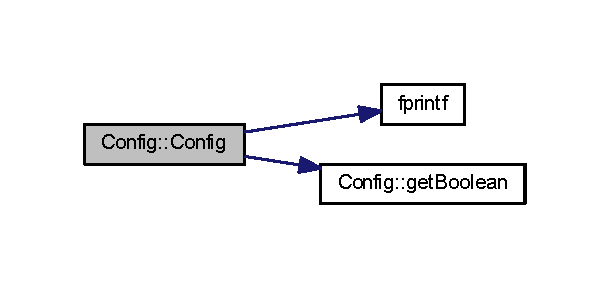
\includegraphics[width=292pt]{class_config_a15f0fb9274e3f774cb6922e2eecf7208_cgraph}
\end{center}
\end{figure}




\subsection{Member Function Documentation}
\hypertarget{class_config_a7d99bbf69b5d0632196a2da20294963c}{\index{Config@{Config}!get\-Boolean@{get\-Boolean}}
\index{get\-Boolean@{get\-Boolean}!Config@{Config}}
\subsubsection[{get\-Boolean}]{\setlength{\rightskip}{0pt plus 5cm}jboolean Config\-::get\-Boolean (
\begin{DoxyParamCaption}
\item[{J\-N\-I\-Env $\ast$}]{jenv, }
\item[{char $\ast$}]{field\-Name}
\end{DoxyParamCaption}
)}}\label{class_config_a7d99bbf69b5d0632196a2da20294963c}


Here is the caller graph for this function\-:
\nopagebreak
\begin{figure}[H]
\begin{center}
\leavevmode
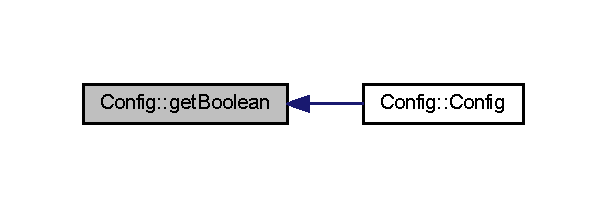
\includegraphics[width=292pt]{class_config_a7d99bbf69b5d0632196a2da20294963c_icgraph}
\end{center}
\end{figure}


\hypertarget{class_config_a6038fb1fbd5089d24afa3b71fd6c0220}{\index{Config@{Config}!is\-Profiling\-C\-S\-V\-Enabled@{is\-Profiling\-C\-S\-V\-Enabled}}
\index{is\-Profiling\-C\-S\-V\-Enabled@{is\-Profiling\-C\-S\-V\-Enabled}!Config@{Config}}
\subsubsection[{is\-Profiling\-C\-S\-V\-Enabled}]{\setlength{\rightskip}{0pt plus 5cm}jboolean Config\-::is\-Profiling\-C\-S\-V\-Enabled (
\begin{DoxyParamCaption}
{}
\end{DoxyParamCaption}
)}}\label{class_config_a6038fb1fbd5089d24afa3b71fd6c0220}


Here is the caller graph for this function\-:
\nopagebreak
\begin{figure}[H]
\begin{center}
\leavevmode
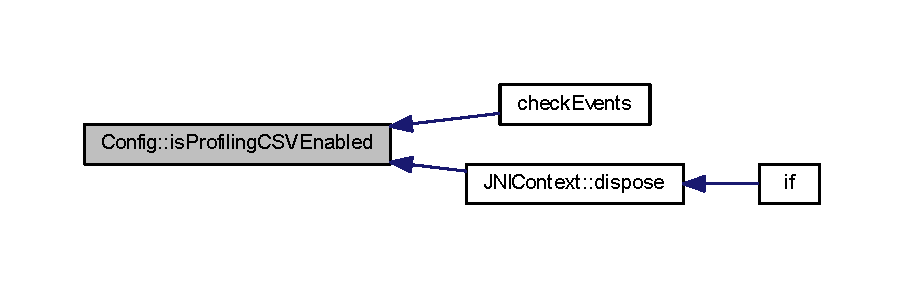
\includegraphics[width=350pt]{class_config_a6038fb1fbd5089d24afa3b71fd6c0220_icgraph}
\end{center}
\end{figure}


\hypertarget{class_config_ac91f68d97d5ca75b787d6ea9cba882e4}{\index{Config@{Config}!is\-Profiling\-Enabled@{is\-Profiling\-Enabled}}
\index{is\-Profiling\-Enabled@{is\-Profiling\-Enabled}!Config@{Config}}
\subsubsection[{is\-Profiling\-Enabled}]{\setlength{\rightskip}{0pt plus 5cm}jboolean Config\-::is\-Profiling\-Enabled (
\begin{DoxyParamCaption}
{}
\end{DoxyParamCaption}
)}}\label{class_config_ac91f68d97d5ca75b787d6ea9cba882e4}


Here is the caller graph for this function\-:
\nopagebreak
\begin{figure}[H]
\begin{center}
\leavevmode
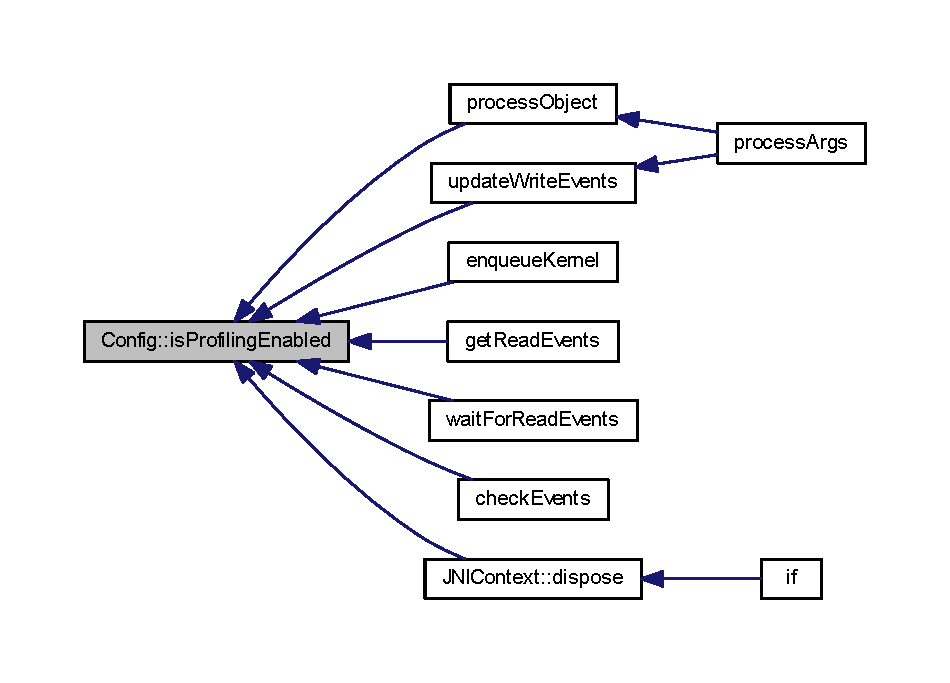
\includegraphics[width=350pt]{class_config_ac91f68d97d5ca75b787d6ea9cba882e4_icgraph}
\end{center}
\end{figure}


\hypertarget{class_config_a7a2cfa5be8d976099dedb684e9c32ca0}{\index{Config@{Config}!is\-Tracking\-Open\-C\-L\-Resources@{is\-Tracking\-Open\-C\-L\-Resources}}
\index{is\-Tracking\-Open\-C\-L\-Resources@{is\-Tracking\-Open\-C\-L\-Resources}!Config@{Config}}
\subsubsection[{is\-Tracking\-Open\-C\-L\-Resources}]{\setlength{\rightskip}{0pt plus 5cm}jboolean Config\-::is\-Tracking\-Open\-C\-L\-Resources (
\begin{DoxyParamCaption}
{}
\end{DoxyParamCaption}
)}}\label{class_config_a7a2cfa5be8d976099dedb684e9c32ca0}


Here is the caller graph for this function\-:
\nopagebreak
\begin{figure}[H]
\begin{center}
\leavevmode
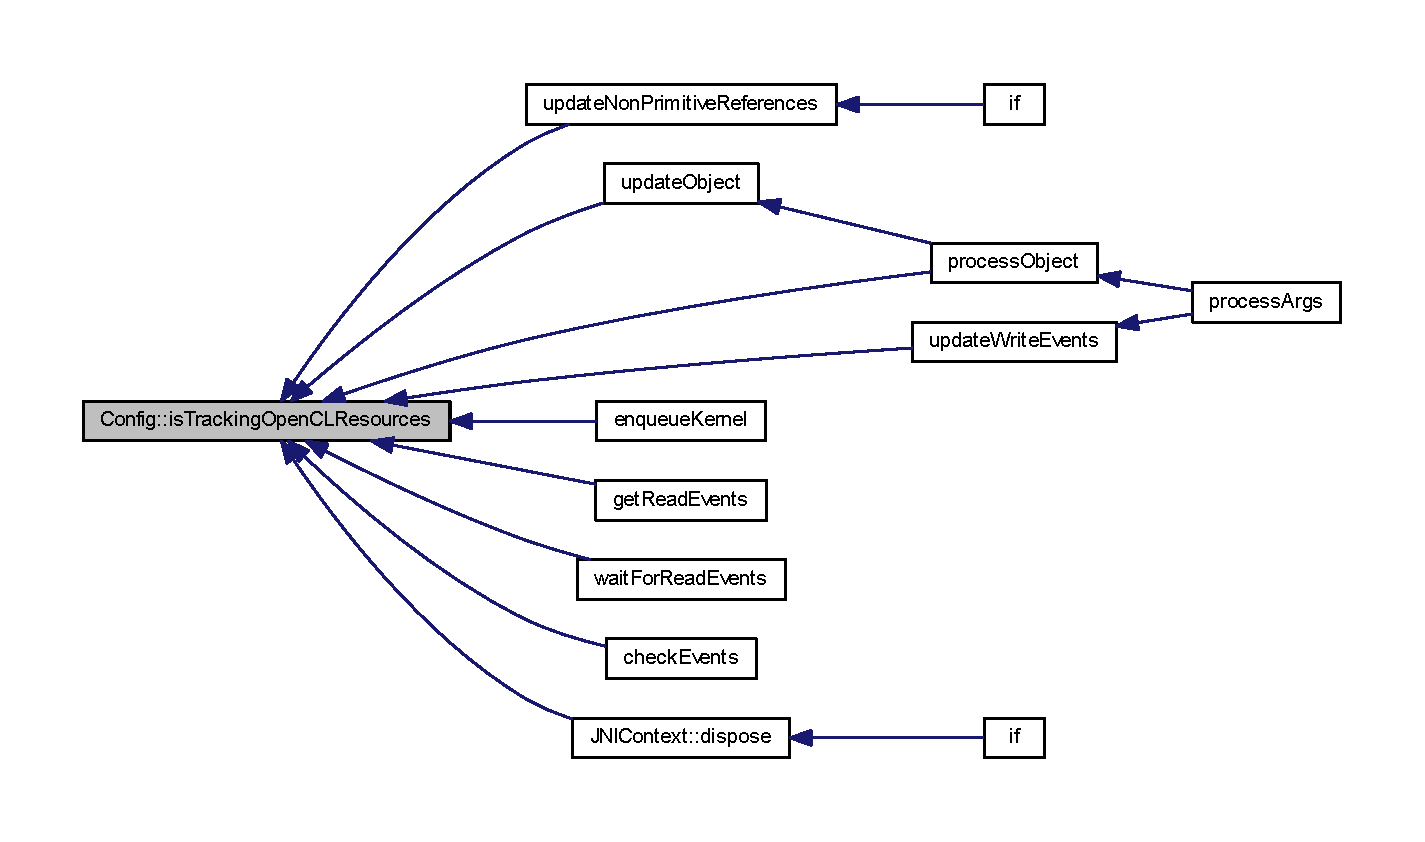
\includegraphics[width=350pt]{class_config_a7a2cfa5be8d976099dedb684e9c32ca0_icgraph}
\end{center}
\end{figure}


\hypertarget{class_config_a03234dbe1adbe1c8fdde649df372926c}{\index{Config@{Config}!is\-Verbose@{is\-Verbose}}
\index{is\-Verbose@{is\-Verbose}!Config@{Config}}
\subsubsection[{is\-Verbose}]{\setlength{\rightskip}{0pt plus 5cm}jboolean Config\-::is\-Verbose (
\begin{DoxyParamCaption}
{}
\end{DoxyParamCaption}
)}}\label{class_config_a03234dbe1adbe1c8fdde649df372926c}


Here is the caller graph for this function\-:
\nopagebreak
\begin{figure}[H]
\begin{center}
\leavevmode
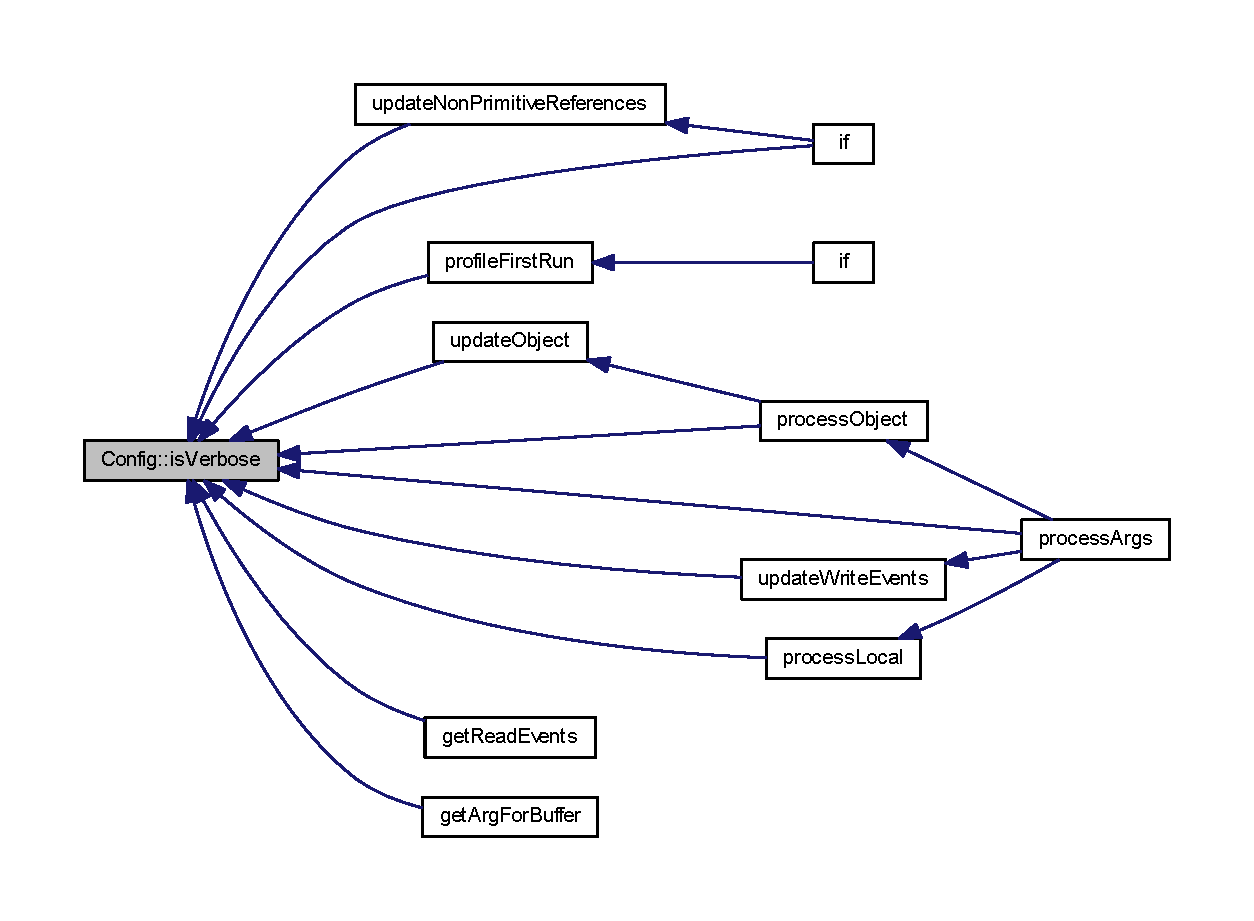
\includegraphics[width=350pt]{class_config_a03234dbe1adbe1c8fdde649df372926c_icgraph}
\end{center}
\end{figure}




\subsection{Member Data Documentation}
\hypertarget{class_config_a7e79ccce393887ace81c263dbc82b0e1}{\index{Config@{Config}!config\-Class@{config\-Class}}
\index{config\-Class@{config\-Class}!Config@{Config}}
\subsubsection[{config\-Class}]{\setlength{\rightskip}{0pt plus 5cm}jclass Config\-::config\-Class}}\label{class_config_a7e79ccce393887ace81c263dbc82b0e1}
\hypertarget{class_config_a84a74c64a238bf8c965c475de0b17124}{\index{Config@{Config}!configured@{configured}}
\index{configured@{configured}!Config@{Config}}
\subsubsection[{configured}]{\setlength{\rightskip}{0pt plus 5cm}jboolean Config\-::configured}}\label{class_config_a84a74c64a238bf8c965c475de0b17124}
\hypertarget{class_config_a403c9cdc52ef31d933ee055d3165a35e}{\index{Config@{Config}!enable\-Profiling@{enable\-Profiling}}
\index{enable\-Profiling@{enable\-Profiling}!Config@{Config}}
\subsubsection[{enable\-Profiling}]{\setlength{\rightskip}{0pt plus 5cm}jboolean Config\-::enable\-Profiling}}\label{class_config_a403c9cdc52ef31d933ee055d3165a35e}
\hypertarget{class_config_afb0e37ad017cbf220fcac529fa644944}{\index{Config@{Config}!enable\-Profiling\-C\-S\-V@{enable\-Profiling\-C\-S\-V}}
\index{enable\-Profiling\-C\-S\-V@{enable\-Profiling\-C\-S\-V}!Config@{Config}}
\subsubsection[{enable\-Profiling\-C\-S\-V}]{\setlength{\rightskip}{0pt plus 5cm}jboolean Config\-::enable\-Profiling\-C\-S\-V}}\label{class_config_afb0e37ad017cbf220fcac529fa644944}
\hypertarget{class_config_af48b23080ff93b7f7720f228715c4eb2}{\index{Config@{Config}!enable\-Verbose\-J\-N\-I@{enable\-Verbose\-J\-N\-I}}
\index{enable\-Verbose\-J\-N\-I@{enable\-Verbose\-J\-N\-I}!Config@{Config}}
\subsubsection[{enable\-Verbose\-J\-N\-I}]{\setlength{\rightskip}{0pt plus 5cm}jboolean Config\-::enable\-Verbose\-J\-N\-I}}\label{class_config_af48b23080ff93b7f7720f228715c4eb2}
\hypertarget{class_config_a40e02509e9330fa8d16087e7dde8a977}{\index{Config@{Config}!enable\-Verbose\-J\-N\-I\-Open\-C\-L\-Resource\-Tracking@{enable\-Verbose\-J\-N\-I\-Open\-C\-L\-Resource\-Tracking}}
\index{enable\-Verbose\-J\-N\-I\-Open\-C\-L\-Resource\-Tracking@{enable\-Verbose\-J\-N\-I\-Open\-C\-L\-Resource\-Tracking}!Config@{Config}}
\subsubsection[{enable\-Verbose\-J\-N\-I\-Open\-C\-L\-Resource\-Tracking}]{\setlength{\rightskip}{0pt plus 5cm}jboolean Config\-::enable\-Verbose\-J\-N\-I\-Open\-C\-L\-Resource\-Tracking}}\label{class_config_a40e02509e9330fa8d16087e7dde8a977}


The documentation for this class was generated from the following files\-:\begin{DoxyCompactItemize}
\item 
src/cpp/run\-Kernel/\hyperlink{config_8h}{config.\-h}\item 
src/cpp/run\-Kernel/\hyperlink{config_8cpp}{config.\-cpp}\end{DoxyCompactItemize}

\hypertarget{class_j_n_i_context}{\section{J\-N\-I\-Context Class Reference}
\label{class_j_n_i_context}\index{J\-N\-I\-Context@{J\-N\-I\-Context}}
}


{\ttfamily \#include $<$J\-N\-I\-Context.\-h$>$}



Collaboration diagram for J\-N\-I\-Context\-:
\nopagebreak
\begin{figure}[H]
\begin{center}
\leavevmode
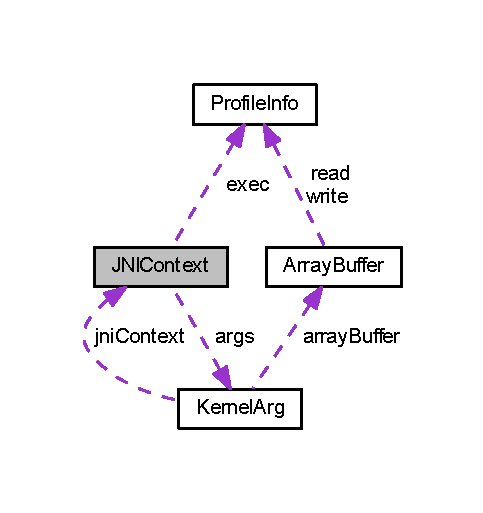
\includegraphics[width=232pt]{class_j_n_i_context__coll__graph}
\end{center}
\end{figure}
\subsection*{Public Member Functions}
\begin{DoxyCompactItemize}
\item 
\hyperlink{class_j_n_i_context_ae7bcb26fc659539d13b21a17e5522477}{J\-N\-I\-Context} (J\-N\-I\-Env $\ast$\hyperlink{aparapi_8cpp_a31595c73e9a3750524b2ff61b5a14f96}{jenv}, jobject \-\_\-kernel\-Object, jobject \-\_\-open\-C\-L\-Device\-Object, jint \-\_\-flags)
\item 
jboolean \hyperlink{class_j_n_i_context_a3d99cd3ef6a15a5f14d765e9c7f471ba}{is\-Valid} ()
\item 
jboolean \hyperlink{class_j_n_i_context_a007f2b45dc1812fc4e3b6c34994d33ec}{is\-Using\-G\-P\-U} ()
\item 
\hyperlink{class_j_n_i_context_adf5347ad76e5f447974741af8b407181}{$\sim$\-J\-N\-I\-Context} ()
\item 
void \hyperlink{class_j_n_i_context_ae0906906c3fe4d7b5c468724bf338903}{dispose} (J\-N\-I\-Env $\ast$\hyperlink{aparapi_8cpp_a31595c73e9a3750524b2ff61b5a14f96}{jenv}, \hyperlink{class_config}{Config} $\ast$\hyperlink{config_8h_a6a44a77efe9d36d03240f900d00dad80}{config})
\item 
void \hyperlink{class_j_n_i_context_a06ec119ce96e3c59c52159976203cbee}{unpin\-All} (J\-N\-I\-Env $\ast$\hyperlink{aparapi_8cpp_a31595c73e9a3750524b2ff61b5a14f96}{jenv})
\end{DoxyCompactItemize}
\subsection*{Static Public Member Functions}
\begin{DoxyCompactItemize}
\item 
static \hyperlink{class_j_n_i_context}{J\-N\-I\-Context} $\ast$ \hyperlink{class_j_n_i_context_acfd6efcf587c0e51bdcc672666a23ed4}{get\-J\-N\-I\-Context} (jlong \hyperlink{aparapi_8cpp_a0040273c7bfca0b191a4ad266d28545d}{jni\-Context\-Handle})
\end{DoxyCompactItemize}
\subsection*{Public Attributes}
\begin{DoxyCompactItemize}
\item 
jobject \hyperlink{class_j_n_i_context_a27e7d5b89e4e4859d15cfc9735e9fdcc}{kernel\-Object}
\item 
jobject \hyperlink{class_j_n_i_context_aecb814e1a3214de3d8f1fc09d93422d6}{open\-C\-L\-Device\-Object}
\item 
jclass \hyperlink{class_j_n_i_context_af91be73a2ebe19dfc194ab58cd9575a9}{kernel\-Class}
\item 
cl\-\_\-device\-\_\-id \hyperlink{class_j_n_i_context_ac9637e5eb4a4de90a76b7a05f1c31882}{device\-Id}
\item 
cl\-\_\-int \hyperlink{class_j_n_i_context_a81fbc7bacb606c79e64a1e03344eb6f3}{device\-Type}
\item 
cl\-\_\-context \hyperlink{class_j_n_i_context_ad405fe75428f606a24260f22a30a4914}{context}
\item 
cl\-\_\-command\-\_\-queue \hyperlink{class_j_n_i_context_af052389a1503633d129ba0a98a8ac94b}{command\-Queue}
\item 
cl\-\_\-program \hyperlink{class_j_n_i_context_a118c4c5f280cb563e4f11727a5fd5664}{program}
\item 
cl\-\_\-kernel \hyperlink{class_j_n_i_context_a845480606129985917deb32c968c5fcd}{kernel}
\item 
jint \hyperlink{class_j_n_i_context_a2a7cb340b07bdc6e1ec3dbee96632747}{argc}
\item 
\hyperlink{class_kernel_arg}{Kernel\-Arg} $\ast$$\ast$ \hyperlink{class_j_n_i_context_ab0dac9ea15c8025e6da69390ee70622c}{args}
\item 
cl\-\_\-event $\ast$ \hyperlink{class_j_n_i_context_aa38ade97cd8becec5edb404d961c6df9}{execute\-Events}
\item 
cl\-\_\-event $\ast$ \hyperlink{class_j_n_i_context_aca766d06dbc6f5deb9086aa12ad3a57e}{read\-Events}
\item 
cl\-\_\-ulong \hyperlink{class_j_n_i_context_ab2562d5b3b5c591b0b8d963306a37cb2}{profile\-Base\-Time}
\item 
jint $\ast$ \hyperlink{class_j_n_i_context_a705ae5bcda4857c3fe95e6781732f8c0}{read\-Event\-Args}
\item 
cl\-\_\-event $\ast$ \hyperlink{class_j_n_i_context_a4b7bcfab666ec64a24ddc5c389fbc3c0}{write\-Events}
\item 
jint $\ast$ \hyperlink{class_j_n_i_context_aabad08832385c27215438477ec4a9429}{write\-Event\-Args}
\item 
jboolean \hyperlink{class_j_n_i_context_a9857a274e84b4de2cd562cd74574b358}{first\-Run}
\item 
jint \hyperlink{class_j_n_i_context_a16c08c772ff54b4cd60524c46f64cafe}{passes}
\item 
\hyperlink{class_profile_info}{Profile\-Info} $\ast$ \hyperlink{class_j_n_i_context_a333bf60d240b3c488933758a3a532857}{exec}
\item 
F\-I\-L\-E $\ast$ \hyperlink{class_j_n_i_context_a88394b796ba1814adc83af940111050b}{profile\-File}
\end{DoxyCompactItemize}
\subsection*{Private Attributes}
\begin{DoxyCompactItemize}
\item 
jint \hyperlink{class_j_n_i_context_a60e21993115f613bef0ab315ae9862e4}{flags}
\item 
jboolean \hyperlink{class_j_n_i_context_a09f80fadd22c3cf5ea45ed979814c1df}{valid}
\end{DoxyCompactItemize}


\subsection{Constructor \& Destructor Documentation}
\hypertarget{class_j_n_i_context_ae7bcb26fc659539d13b21a17e5522477}{\index{J\-N\-I\-Context@{J\-N\-I\-Context}!J\-N\-I\-Context@{J\-N\-I\-Context}}
\index{J\-N\-I\-Context@{J\-N\-I\-Context}!JNIContext@{J\-N\-I\-Context}}
\subsubsection[{J\-N\-I\-Context}]{\setlength{\rightskip}{0pt plus 5cm}J\-N\-I\-Context\-::\-J\-N\-I\-Context (
\begin{DoxyParamCaption}
\item[{J\-N\-I\-Env $\ast$}]{jenv, }
\item[{jobject}]{\-\_\-kernel\-Object, }
\item[{jobject}]{\-\_\-open\-C\-L\-Device\-Object, }
\item[{jint}]{\-\_\-flags}
\end{DoxyParamCaption}
)}}\label{class_j_n_i_context_ae7bcb26fc659539d13b21a17e5522477}


Here is the call graph for this function\-:
\nopagebreak
\begin{figure}[H]
\begin{center}
\leavevmode
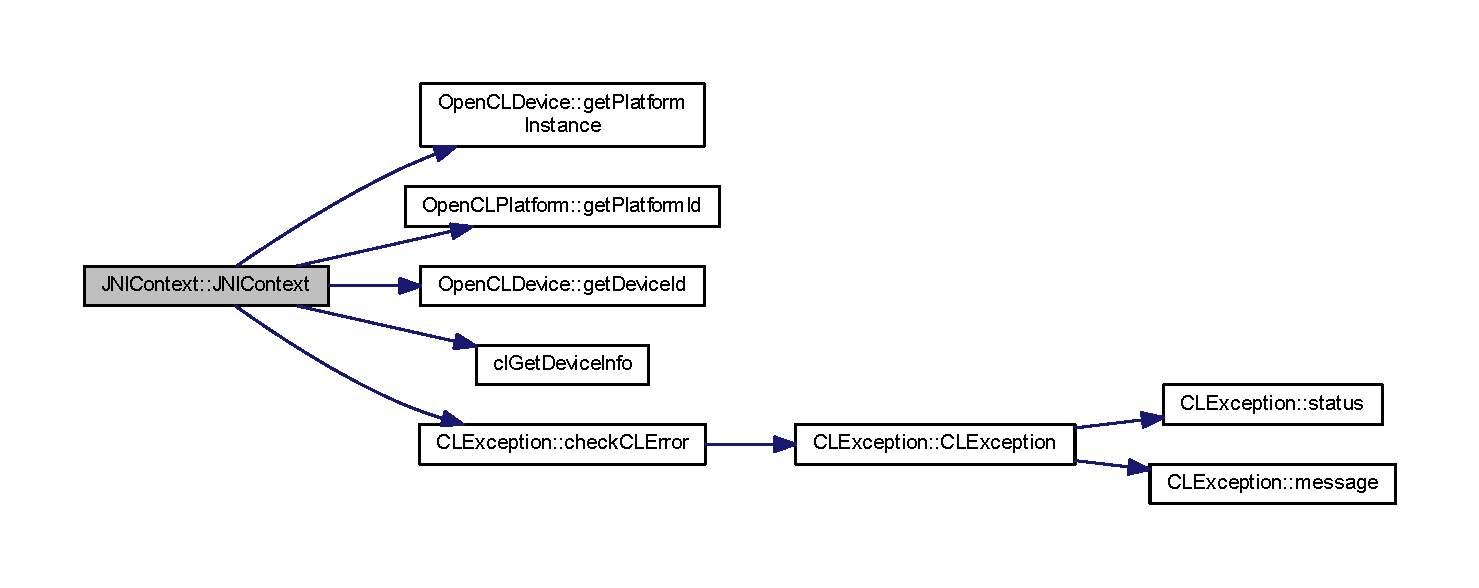
\includegraphics[width=350pt]{class_j_n_i_context_ae7bcb26fc659539d13b21a17e5522477_cgraph}
\end{center}
\end{figure}


\hypertarget{class_j_n_i_context_adf5347ad76e5f447974741af8b407181}{\index{J\-N\-I\-Context@{J\-N\-I\-Context}!$\sim$\-J\-N\-I\-Context@{$\sim$\-J\-N\-I\-Context}}
\index{$\sim$\-J\-N\-I\-Context@{$\sim$\-J\-N\-I\-Context}!JNIContext@{J\-N\-I\-Context}}
\subsubsection[{$\sim$\-J\-N\-I\-Context}]{\setlength{\rightskip}{0pt plus 5cm}J\-N\-I\-Context\-::$\sim$\-J\-N\-I\-Context (
\begin{DoxyParamCaption}
{}
\end{DoxyParamCaption}
)\hspace{0.3cm}{\ttfamily [inline]}}}\label{class_j_n_i_context_adf5347ad76e5f447974741af8b407181}


\subsection{Member Function Documentation}
\hypertarget{class_j_n_i_context_ae0906906c3fe4d7b5c468724bf338903}{\index{J\-N\-I\-Context@{J\-N\-I\-Context}!dispose@{dispose}}
\index{dispose@{dispose}!JNIContext@{J\-N\-I\-Context}}
\subsubsection[{dispose}]{\setlength{\rightskip}{0pt plus 5cm}void J\-N\-I\-Context\-::dispose (
\begin{DoxyParamCaption}
\item[{J\-N\-I\-Env $\ast$}]{jenv, }
\item[{{\bf Config} $\ast$}]{config}
\end{DoxyParamCaption}
)}}\label{class_j_n_i_context_ae0906906c3fe4d7b5c468724bf338903}


Here is the call graph for this function\-:
\nopagebreak
\begin{figure}[H]
\begin{center}
\leavevmode
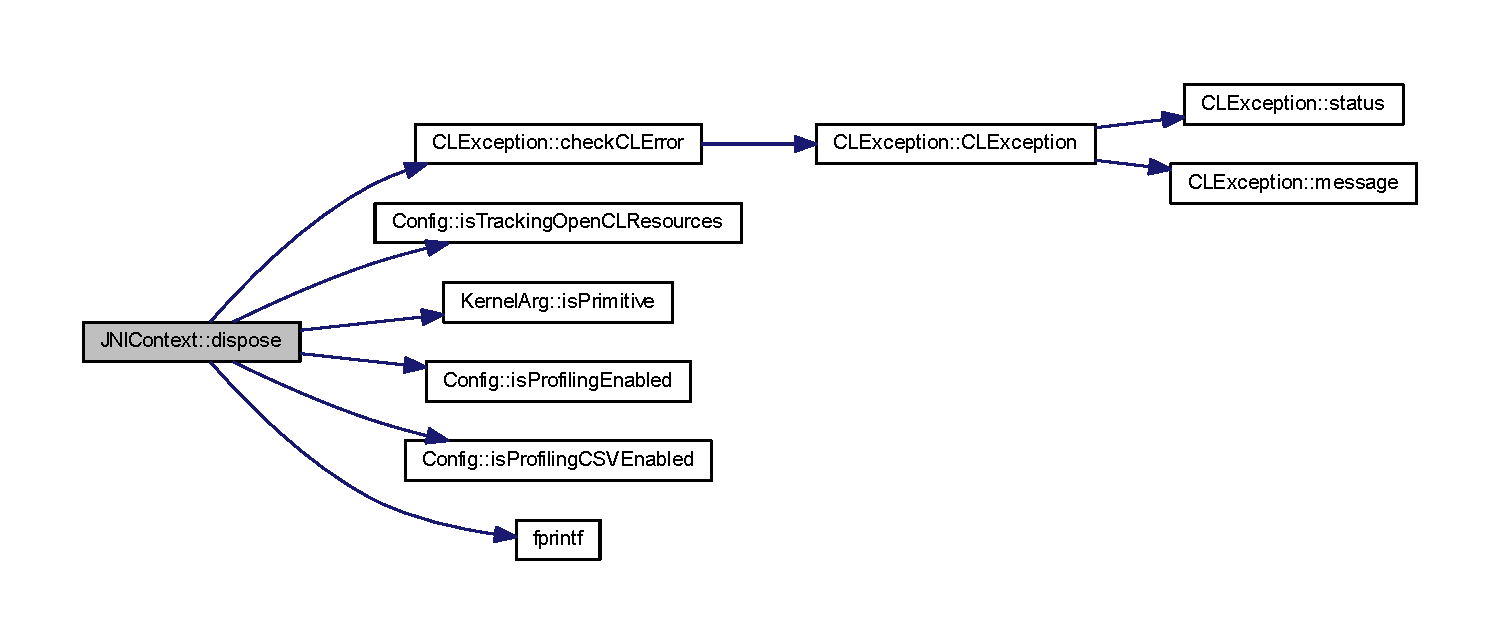
\includegraphics[width=350pt]{class_j_n_i_context_ae0906906c3fe4d7b5c468724bf338903_cgraph}
\end{center}
\end{figure}




Here is the caller graph for this function\-:
\nopagebreak
\begin{figure}[H]
\begin{center}
\leavevmode
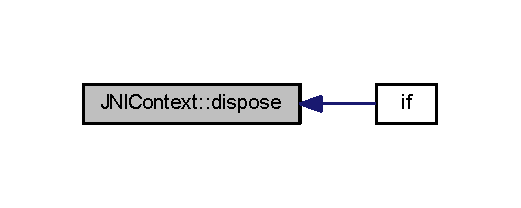
\includegraphics[width=250pt]{class_j_n_i_context_ae0906906c3fe4d7b5c468724bf338903_icgraph}
\end{center}
\end{figure}


\hypertarget{class_j_n_i_context_acfd6efcf587c0e51bdcc672666a23ed4}{\index{J\-N\-I\-Context@{J\-N\-I\-Context}!get\-J\-N\-I\-Context@{get\-J\-N\-I\-Context}}
\index{get\-J\-N\-I\-Context@{get\-J\-N\-I\-Context}!JNIContext@{J\-N\-I\-Context}}
\subsubsection[{get\-J\-N\-I\-Context}]{\setlength{\rightskip}{0pt plus 5cm}static {\bf J\-N\-I\-Context}$\ast$ J\-N\-I\-Context\-::get\-J\-N\-I\-Context (
\begin{DoxyParamCaption}
\item[{jlong}]{jni\-Context\-Handle}
\end{DoxyParamCaption}
)\hspace{0.3cm}{\ttfamily [inline]}, {\ttfamily [static]}}}\label{class_j_n_i_context_acfd6efcf587c0e51bdcc672666a23ed4}
\hypertarget{class_j_n_i_context_a007f2b45dc1812fc4e3b6c34994d33ec}{\index{J\-N\-I\-Context@{J\-N\-I\-Context}!is\-Using\-G\-P\-U@{is\-Using\-G\-P\-U}}
\index{is\-Using\-G\-P\-U@{is\-Using\-G\-P\-U}!JNIContext@{J\-N\-I\-Context}}
\subsubsection[{is\-Using\-G\-P\-U}]{\setlength{\rightskip}{0pt plus 5cm}jboolean J\-N\-I\-Context\-::is\-Using\-G\-P\-U (
\begin{DoxyParamCaption}
{}
\end{DoxyParamCaption}
)\hspace{0.3cm}{\ttfamily [inline]}}}\label{class_j_n_i_context_a007f2b45dc1812fc4e3b6c34994d33ec}
\hypertarget{class_j_n_i_context_a3d99cd3ef6a15a5f14d765e9c7f471ba}{\index{J\-N\-I\-Context@{J\-N\-I\-Context}!is\-Valid@{is\-Valid}}
\index{is\-Valid@{is\-Valid}!JNIContext@{J\-N\-I\-Context}}
\subsubsection[{is\-Valid}]{\setlength{\rightskip}{0pt plus 5cm}jboolean J\-N\-I\-Context\-::is\-Valid (
\begin{DoxyParamCaption}
{}
\end{DoxyParamCaption}
)\hspace{0.3cm}{\ttfamily [inline]}}}\label{class_j_n_i_context_a3d99cd3ef6a15a5f14d765e9c7f471ba}
\hypertarget{class_j_n_i_context_a06ec119ce96e3c59c52159976203cbee}{\index{J\-N\-I\-Context@{J\-N\-I\-Context}!unpin\-All@{unpin\-All}}
\index{unpin\-All@{unpin\-All}!JNIContext@{J\-N\-I\-Context}}
\subsubsection[{unpin\-All}]{\setlength{\rightskip}{0pt plus 5cm}void J\-N\-I\-Context\-::unpin\-All (
\begin{DoxyParamCaption}
\item[{J\-N\-I\-Env $\ast$}]{jenv}
\end{DoxyParamCaption}
)}}\label{class_j_n_i_context_a06ec119ce96e3c59c52159976203cbee}
Release J\-N\-I critical pinned arrays before returning to java code 

Here is the call graph for this function\-:
\nopagebreak
\begin{figure}[H]
\begin{center}
\leavevmode
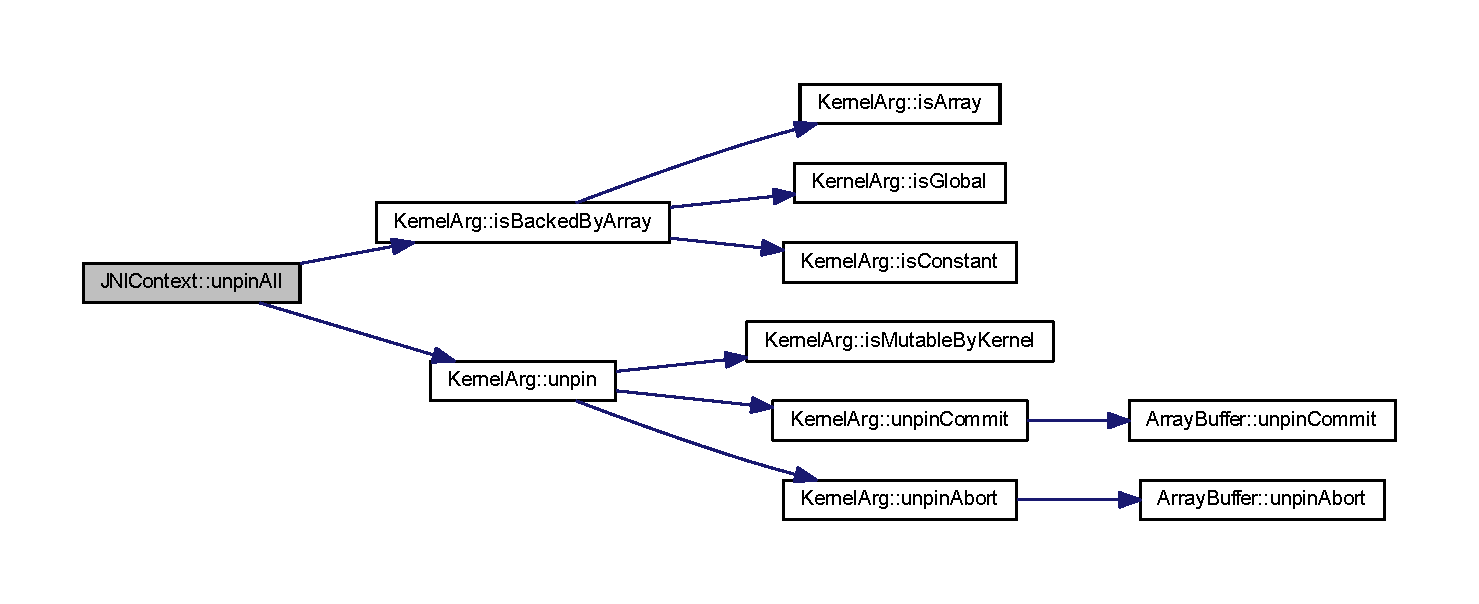
\includegraphics[width=350pt]{class_j_n_i_context_a06ec119ce96e3c59c52159976203cbee_cgraph}
\end{center}
\end{figure}




Here is the caller graph for this function\-:
\nopagebreak
\begin{figure}[H]
\begin{center}
\leavevmode
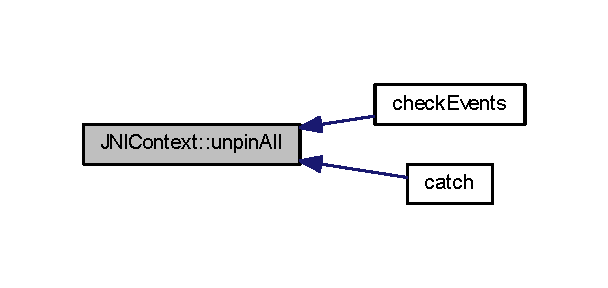
\includegraphics[width=292pt]{class_j_n_i_context_a06ec119ce96e3c59c52159976203cbee_icgraph}
\end{center}
\end{figure}




\subsection{Member Data Documentation}
\hypertarget{class_j_n_i_context_a2a7cb340b07bdc6e1ec3dbee96632747}{\index{J\-N\-I\-Context@{J\-N\-I\-Context}!argc@{argc}}
\index{argc@{argc}!JNIContext@{J\-N\-I\-Context}}
\subsubsection[{argc}]{\setlength{\rightskip}{0pt plus 5cm}jint J\-N\-I\-Context\-::argc}}\label{class_j_n_i_context_a2a7cb340b07bdc6e1ec3dbee96632747}
\hypertarget{class_j_n_i_context_ab0dac9ea15c8025e6da69390ee70622c}{\index{J\-N\-I\-Context@{J\-N\-I\-Context}!args@{args}}
\index{args@{args}!JNIContext@{J\-N\-I\-Context}}
\subsubsection[{args}]{\setlength{\rightskip}{0pt plus 5cm}{\bf Kernel\-Arg}$\ast$$\ast$ J\-N\-I\-Context\-::args}}\label{class_j_n_i_context_ab0dac9ea15c8025e6da69390ee70622c}
\hypertarget{class_j_n_i_context_af052389a1503633d129ba0a98a8ac94b}{\index{J\-N\-I\-Context@{J\-N\-I\-Context}!command\-Queue@{command\-Queue}}
\index{command\-Queue@{command\-Queue}!JNIContext@{J\-N\-I\-Context}}
\subsubsection[{command\-Queue}]{\setlength{\rightskip}{0pt plus 5cm}cl\-\_\-command\-\_\-queue J\-N\-I\-Context\-::command\-Queue}}\label{class_j_n_i_context_af052389a1503633d129ba0a98a8ac94b}
\hypertarget{class_j_n_i_context_ad405fe75428f606a24260f22a30a4914}{\index{J\-N\-I\-Context@{J\-N\-I\-Context}!context@{context}}
\index{context@{context}!JNIContext@{J\-N\-I\-Context}}
\subsubsection[{context}]{\setlength{\rightskip}{0pt plus 5cm}cl\-\_\-context J\-N\-I\-Context\-::context}}\label{class_j_n_i_context_ad405fe75428f606a24260f22a30a4914}
\hypertarget{class_j_n_i_context_ac9637e5eb4a4de90a76b7a05f1c31882}{\index{J\-N\-I\-Context@{J\-N\-I\-Context}!device\-Id@{device\-Id}}
\index{device\-Id@{device\-Id}!JNIContext@{J\-N\-I\-Context}}
\subsubsection[{device\-Id}]{\setlength{\rightskip}{0pt plus 5cm}cl\-\_\-device\-\_\-id J\-N\-I\-Context\-::device\-Id}}\label{class_j_n_i_context_ac9637e5eb4a4de90a76b7a05f1c31882}
\hypertarget{class_j_n_i_context_a81fbc7bacb606c79e64a1e03344eb6f3}{\index{J\-N\-I\-Context@{J\-N\-I\-Context}!device\-Type@{device\-Type}}
\index{device\-Type@{device\-Type}!JNIContext@{J\-N\-I\-Context}}
\subsubsection[{device\-Type}]{\setlength{\rightskip}{0pt plus 5cm}cl\-\_\-int J\-N\-I\-Context\-::device\-Type}}\label{class_j_n_i_context_a81fbc7bacb606c79e64a1e03344eb6f3}
\hypertarget{class_j_n_i_context_a333bf60d240b3c488933758a3a532857}{\index{J\-N\-I\-Context@{J\-N\-I\-Context}!exec@{exec}}
\index{exec@{exec}!JNIContext@{J\-N\-I\-Context}}
\subsubsection[{exec}]{\setlength{\rightskip}{0pt plus 5cm}{\bf Profile\-Info}$\ast$ J\-N\-I\-Context\-::exec}}\label{class_j_n_i_context_a333bf60d240b3c488933758a3a532857}
\hypertarget{class_j_n_i_context_aa38ade97cd8becec5edb404d961c6df9}{\index{J\-N\-I\-Context@{J\-N\-I\-Context}!execute\-Events@{execute\-Events}}
\index{execute\-Events@{execute\-Events}!JNIContext@{J\-N\-I\-Context}}
\subsubsection[{execute\-Events}]{\setlength{\rightskip}{0pt plus 5cm}cl\-\_\-event$\ast$ J\-N\-I\-Context\-::execute\-Events}}\label{class_j_n_i_context_aa38ade97cd8becec5edb404d961c6df9}
\hypertarget{class_j_n_i_context_a9857a274e84b4de2cd562cd74574b358}{\index{J\-N\-I\-Context@{J\-N\-I\-Context}!first\-Run@{first\-Run}}
\index{first\-Run@{first\-Run}!JNIContext@{J\-N\-I\-Context}}
\subsubsection[{first\-Run}]{\setlength{\rightskip}{0pt plus 5cm}jboolean J\-N\-I\-Context\-::first\-Run}}\label{class_j_n_i_context_a9857a274e84b4de2cd562cd74574b358}
\hypertarget{class_j_n_i_context_a60e21993115f613bef0ab315ae9862e4}{\index{J\-N\-I\-Context@{J\-N\-I\-Context}!flags@{flags}}
\index{flags@{flags}!JNIContext@{J\-N\-I\-Context}}
\subsubsection[{flags}]{\setlength{\rightskip}{0pt plus 5cm}jint J\-N\-I\-Context\-::flags\hspace{0.3cm}{\ttfamily [private]}}}\label{class_j_n_i_context_a60e21993115f613bef0ab315ae9862e4}
\hypertarget{class_j_n_i_context_a845480606129985917deb32c968c5fcd}{\index{J\-N\-I\-Context@{J\-N\-I\-Context}!kernel@{kernel}}
\index{kernel@{kernel}!JNIContext@{J\-N\-I\-Context}}
\subsubsection[{kernel}]{\setlength{\rightskip}{0pt plus 5cm}cl\-\_\-kernel J\-N\-I\-Context\-::kernel}}\label{class_j_n_i_context_a845480606129985917deb32c968c5fcd}
\hypertarget{class_j_n_i_context_af91be73a2ebe19dfc194ab58cd9575a9}{\index{J\-N\-I\-Context@{J\-N\-I\-Context}!kernel\-Class@{kernel\-Class}}
\index{kernel\-Class@{kernel\-Class}!JNIContext@{J\-N\-I\-Context}}
\subsubsection[{kernel\-Class}]{\setlength{\rightskip}{0pt plus 5cm}jclass J\-N\-I\-Context\-::kernel\-Class}}\label{class_j_n_i_context_af91be73a2ebe19dfc194ab58cd9575a9}
\hypertarget{class_j_n_i_context_a27e7d5b89e4e4859d15cfc9735e9fdcc}{\index{J\-N\-I\-Context@{J\-N\-I\-Context}!kernel\-Object@{kernel\-Object}}
\index{kernel\-Object@{kernel\-Object}!JNIContext@{J\-N\-I\-Context}}
\subsubsection[{kernel\-Object}]{\setlength{\rightskip}{0pt plus 5cm}jobject J\-N\-I\-Context\-::kernel\-Object}}\label{class_j_n_i_context_a27e7d5b89e4e4859d15cfc9735e9fdcc}
\hypertarget{class_j_n_i_context_aecb814e1a3214de3d8f1fc09d93422d6}{\index{J\-N\-I\-Context@{J\-N\-I\-Context}!open\-C\-L\-Device\-Object@{open\-C\-L\-Device\-Object}}
\index{open\-C\-L\-Device\-Object@{open\-C\-L\-Device\-Object}!JNIContext@{J\-N\-I\-Context}}
\subsubsection[{open\-C\-L\-Device\-Object}]{\setlength{\rightskip}{0pt plus 5cm}jobject J\-N\-I\-Context\-::open\-C\-L\-Device\-Object}}\label{class_j_n_i_context_aecb814e1a3214de3d8f1fc09d93422d6}
\hypertarget{class_j_n_i_context_a16c08c772ff54b4cd60524c46f64cafe}{\index{J\-N\-I\-Context@{J\-N\-I\-Context}!passes@{passes}}
\index{passes@{passes}!JNIContext@{J\-N\-I\-Context}}
\subsubsection[{passes}]{\setlength{\rightskip}{0pt plus 5cm}jint J\-N\-I\-Context\-::passes}}\label{class_j_n_i_context_a16c08c772ff54b4cd60524c46f64cafe}
\hypertarget{class_j_n_i_context_ab2562d5b3b5c591b0b8d963306a37cb2}{\index{J\-N\-I\-Context@{J\-N\-I\-Context}!profile\-Base\-Time@{profile\-Base\-Time}}
\index{profile\-Base\-Time@{profile\-Base\-Time}!JNIContext@{J\-N\-I\-Context}}
\subsubsection[{profile\-Base\-Time}]{\setlength{\rightskip}{0pt plus 5cm}cl\-\_\-ulong J\-N\-I\-Context\-::profile\-Base\-Time}}\label{class_j_n_i_context_ab2562d5b3b5c591b0b8d963306a37cb2}
\hypertarget{class_j_n_i_context_a88394b796ba1814adc83af940111050b}{\index{J\-N\-I\-Context@{J\-N\-I\-Context}!profile\-File@{profile\-File}}
\index{profile\-File@{profile\-File}!JNIContext@{J\-N\-I\-Context}}
\subsubsection[{profile\-File}]{\setlength{\rightskip}{0pt plus 5cm}F\-I\-L\-E$\ast$ J\-N\-I\-Context\-::profile\-File}}\label{class_j_n_i_context_a88394b796ba1814adc83af940111050b}
\hypertarget{class_j_n_i_context_a118c4c5f280cb563e4f11727a5fd5664}{\index{J\-N\-I\-Context@{J\-N\-I\-Context}!program@{program}}
\index{program@{program}!JNIContext@{J\-N\-I\-Context}}
\subsubsection[{program}]{\setlength{\rightskip}{0pt plus 5cm}cl\-\_\-program J\-N\-I\-Context\-::program}}\label{class_j_n_i_context_a118c4c5f280cb563e4f11727a5fd5664}
\hypertarget{class_j_n_i_context_a705ae5bcda4857c3fe95e6781732f8c0}{\index{J\-N\-I\-Context@{J\-N\-I\-Context}!read\-Event\-Args@{read\-Event\-Args}}
\index{read\-Event\-Args@{read\-Event\-Args}!JNIContext@{J\-N\-I\-Context}}
\subsubsection[{read\-Event\-Args}]{\setlength{\rightskip}{0pt plus 5cm}jint$\ast$ J\-N\-I\-Context\-::read\-Event\-Args}}\label{class_j_n_i_context_a705ae5bcda4857c3fe95e6781732f8c0}
\hypertarget{class_j_n_i_context_aca766d06dbc6f5deb9086aa12ad3a57e}{\index{J\-N\-I\-Context@{J\-N\-I\-Context}!read\-Events@{read\-Events}}
\index{read\-Events@{read\-Events}!JNIContext@{J\-N\-I\-Context}}
\subsubsection[{read\-Events}]{\setlength{\rightskip}{0pt plus 5cm}cl\-\_\-event$\ast$ J\-N\-I\-Context\-::read\-Events}}\label{class_j_n_i_context_aca766d06dbc6f5deb9086aa12ad3a57e}
\hypertarget{class_j_n_i_context_a09f80fadd22c3cf5ea45ed979814c1df}{\index{J\-N\-I\-Context@{J\-N\-I\-Context}!valid@{valid}}
\index{valid@{valid}!JNIContext@{J\-N\-I\-Context}}
\subsubsection[{valid}]{\setlength{\rightskip}{0pt plus 5cm}jboolean J\-N\-I\-Context\-::valid\hspace{0.3cm}{\ttfamily [private]}}}\label{class_j_n_i_context_a09f80fadd22c3cf5ea45ed979814c1df}
\hypertarget{class_j_n_i_context_aabad08832385c27215438477ec4a9429}{\index{J\-N\-I\-Context@{J\-N\-I\-Context}!write\-Event\-Args@{write\-Event\-Args}}
\index{write\-Event\-Args@{write\-Event\-Args}!JNIContext@{J\-N\-I\-Context}}
\subsubsection[{write\-Event\-Args}]{\setlength{\rightskip}{0pt plus 5cm}jint$\ast$ J\-N\-I\-Context\-::write\-Event\-Args}}\label{class_j_n_i_context_aabad08832385c27215438477ec4a9429}
\hypertarget{class_j_n_i_context_a4b7bcfab666ec64a24ddc5c389fbc3c0}{\index{J\-N\-I\-Context@{J\-N\-I\-Context}!write\-Events@{write\-Events}}
\index{write\-Events@{write\-Events}!JNIContext@{J\-N\-I\-Context}}
\subsubsection[{write\-Events}]{\setlength{\rightskip}{0pt plus 5cm}cl\-\_\-event$\ast$ J\-N\-I\-Context\-::write\-Events}}\label{class_j_n_i_context_a4b7bcfab666ec64a24ddc5c389fbc3c0}


The documentation for this class was generated from the following files\-:\begin{DoxyCompactItemize}
\item 
src/cpp/run\-Kernel/\hyperlink{_j_n_i_context_8h}{J\-N\-I\-Context.\-h}\item 
src/cpp/run\-Kernel/\hyperlink{_j_n_i_context_8cpp}{J\-N\-I\-Context.\-cpp}\end{DoxyCompactItemize}

\hypertarget{class_j_n_i_helper}{\section{J\-N\-I\-Helper Class Reference}
\label{class_j_n_i_helper}\index{J\-N\-I\-Helper@{J\-N\-I\-Helper}}
}


{\ttfamily \#include $<$jni\-Helper.\-h$>$}

\subsection*{Static Public Member Functions}
\begin{DoxyCompactItemize}
\item 
static void \hyperlink{class_j_n_i_helper_adff29cbca25d5f6787f675afcdc38871}{call\-Void} (J\-N\-I\-Env $\ast$\hyperlink{aparapi_8cpp_a31595c73e9a3750524b2ff61b5a14f96}{jenv}, jobject instance, char $\ast$method\-Name, char $\ast$method\-Signature,...)
\item 
static jlong \hyperlink{class_j_n_i_helper_a0c2378b0f3447af66038ae9f6dea1000}{call\-Long} (J\-N\-I\-Env $\ast$\hyperlink{aparapi_8cpp_a31595c73e9a3750524b2ff61b5a14f96}{jenv}, jobject instance, char $\ast$method\-Name, char $\ast$method\-Signature,...)
\item 
static jobject \hyperlink{class_j_n_i_helper_ac6fc439bd0a306c475cc1392ff586951}{call\-Object} (J\-N\-I\-Env $\ast$\hyperlink{aparapi_8cpp_a31595c73e9a3750524b2ff61b5a14f96}{jenv}, jobject instance, char $\ast$method\-Name, char $\ast$method\-Signature,...)
\item 
static jobject \hyperlink{class_j_n_i_helper_a6d0240a89937c774bd5229944a54a544}{create\-Instance} (J\-N\-I\-Env $\ast$\hyperlink{aparapi_8cpp_a31595c73e9a3750524b2ff61b5a14f96}{jenv}, char $\ast$class\-Name, char $\ast$signature,...)
\item 
static jobject \hyperlink{class_j_n_i_helper_a62620661bbb5a7eb1c38cedccb2d9066}{get\-Static\-Field\-Object} (J\-N\-I\-Env $\ast$\hyperlink{aparapi_8cpp_a31595c73e9a3750524b2ff61b5a14f96}{jenv}, char $\ast$class\-Name, char $\ast$field\-Name, char $\ast$signature)
\item 
static std\-::string \hyperlink{class_j_n_i_helper_a6934bf9b61e058225184032cfc49bf08}{get\-Type} (jint value)
\item 
static std\-::string \hyperlink{class_j_n_i_helper_a3d4a3261b07e28a398bd99d59deb4160}{get\-Type} (jfloat value)
\item 
static std\-::string \hyperlink{class_j_n_i_helper_ad781e04f8719bcfa2a33868867a2a4b5}{get\-Type} (jdouble value)
\item 
static std\-::string \hyperlink{class_j_n_i_helper_a206d661817dd7011bf611e2c52160d59}{get\-Type} (jshort value)
\item 
static std\-::string \hyperlink{class_j_n_i_helper_a2a101aa6ff2af7a1ca5d80be913ea46a}{get\-Type} (jlong value)
\item 
static std\-::string \hyperlink{class_j_n_i_helper_a89e129b46a8d1cdee4e9ac5840d42f30}{get\-Type} (jobject value)
\item 
static std\-::string \hyperlink{class_j_n_i_helper_a777e896380d762f15c61c051907fa98d}{get\-Type} (jboolean value)
\item 
{\footnotesize template$<$typename j\-T $>$ }\\static void \hyperlink{class_j_n_i_helper_a950f746b15f97df78e3150de33c16422}{set\-Instance\-Field} (J\-N\-I\-Env $\ast$\hyperlink{aparapi_8cpp_a31595c73e9a3750524b2ff61b5a14f96}{jenv}, jobject instance, const char $\ast$field\-Name, j\-T value)
\item 
{\footnotesize template$<$typename j\-T $>$ }\\static void \hyperlink{class_j_n_i_helper_aecce0e924d9c77e74e09220ba3112c87}{set\-Instance\-Field} (J\-N\-I\-Env $\ast$\hyperlink{aparapi_8cpp_a31595c73e9a3750524b2ff61b5a14f96}{jenv}, jobject instance, const char $\ast$field\-Name, const char $\ast$signature, j\-T value)
\item 
{\footnotesize template$<$typename j\-T $>$ }\\static j\-T \hyperlink{class_j_n_i_helper_a1c640a98f51b1ace46bd99c8c1a75557}{get\-Instance\-Field} (J\-N\-I\-Env $\ast$\hyperlink{aparapi_8cpp_a31595c73e9a3750524b2ff61b5a14f96}{jenv}, jobject instance, const char $\ast$field\-Name)
\item 
{\footnotesize template$<$typename j\-T $>$ }\\static j\-T \hyperlink{class_j_n_i_helper_a1840235841c1159432d86a7a545564bd}{get\-Instance\-Field} (J\-N\-I\-Env $\ast$\hyperlink{aparapi_8cpp_a31595c73e9a3750524b2ff61b5a14f96}{jenv}, jobject instance, const char $\ast$field\-Name, const char $\ast$signature)
\item 
static jfield\-I\-D \hyperlink{class_j_n_i_helper_adc97179237bf9d5b36d06663c6bbc074}{Get\-Field\-I\-D} (J\-N\-I\-Env $\ast$\hyperlink{aparapi_8cpp_a31595c73e9a3750524b2ff61b5a14f96}{jenv}, jclass c, const char $\ast$name, const char $\ast$type)
\end{DoxyCompactItemize}
\subsection*{Static Private Member Functions}
\begin{DoxyCompactItemize}
\item 
static void \hyperlink{class_j_n_i_helper_a8265ea28e2311aac6a66a2b794b4a8fe}{set\-Field} (J\-N\-I\-Env $\ast$\hyperlink{aparapi_8cpp_a31595c73e9a3750524b2ff61b5a14f96}{jenv}, jobject instance, jfield\-I\-D field\-Id, jint $\ast$value)
\item 
static void \hyperlink{class_j_n_i_helper_a6a24cbc36c6c00c8062735b872c9ddb5}{set\-Field} (J\-N\-I\-Env $\ast$\hyperlink{aparapi_8cpp_a31595c73e9a3750524b2ff61b5a14f96}{jenv}, jobject instance, jfield\-I\-D field\-Id, jfloat $\ast$value)
\item 
static void \hyperlink{class_j_n_i_helper_a91745290d3dbba0bc0e899a2e4cbb0b3}{set\-Field} (J\-N\-I\-Env $\ast$\hyperlink{aparapi_8cpp_a31595c73e9a3750524b2ff61b5a14f96}{jenv}, jobject instance, jfield\-I\-D field\-Id, jdouble $\ast$value)
\item 
static void \hyperlink{class_j_n_i_helper_a707937851d5e36013feb79dd29e79978}{set\-Field} (J\-N\-I\-Env $\ast$\hyperlink{aparapi_8cpp_a31595c73e9a3750524b2ff61b5a14f96}{jenv}, jobject instance, jfield\-I\-D field\-Id, jshort $\ast$value)
\item 
static void \hyperlink{class_j_n_i_helper_ae1272f3e616aed8c1ba6ba775e73dc7d}{set\-Field} (J\-N\-I\-Env $\ast$\hyperlink{aparapi_8cpp_a31595c73e9a3750524b2ff61b5a14f96}{jenv}, jobject instance, jfield\-I\-D field\-Id, jlong $\ast$value)
\item 
static void \hyperlink{class_j_n_i_helper_a135376558da387f45f147c1d32cd5c21}{set\-Field} (J\-N\-I\-Env $\ast$\hyperlink{aparapi_8cpp_a31595c73e9a3750524b2ff61b5a14f96}{jenv}, jobject instance, jfield\-I\-D field\-Id, jobject $\ast$value)
\item 
static void \hyperlink{class_j_n_i_helper_a53481dbf082667c76aff43e32e90bdf6}{set\-Field} (J\-N\-I\-Env $\ast$\hyperlink{aparapi_8cpp_a31595c73e9a3750524b2ff61b5a14f96}{jenv}, jobject instance, jfield\-I\-D field\-Id, jboolean $\ast$value)
\item 
static void \hyperlink{class_j_n_i_helper_ad389729ad0900ed6f3ccc7a105e42c9a}{get\-Field} (J\-N\-I\-Env $\ast$\hyperlink{aparapi_8cpp_a31595c73e9a3750524b2ff61b5a14f96}{jenv}, jobject instance, jfield\-I\-D field\-Id, jint $\ast$value)
\item 
static void \hyperlink{class_j_n_i_helper_aca90dfc2fcb39564f82a66cf01a8d4f6}{get\-Field} (J\-N\-I\-Env $\ast$\hyperlink{aparapi_8cpp_a31595c73e9a3750524b2ff61b5a14f96}{jenv}, jobject instance, jfield\-I\-D field\-Id, jfloat $\ast$value)
\item 
static void \hyperlink{class_j_n_i_helper_a39cebd8486f32528314d28ecb1f709ca}{get\-Field} (J\-N\-I\-Env $\ast$\hyperlink{aparapi_8cpp_a31595c73e9a3750524b2ff61b5a14f96}{jenv}, jobject instance, jfield\-I\-D field\-Id, jdouble $\ast$value)
\item 
static void \hyperlink{class_j_n_i_helper_a232126b247a62164c157494aaa7e8486}{get\-Field} (J\-N\-I\-Env $\ast$\hyperlink{aparapi_8cpp_a31595c73e9a3750524b2ff61b5a14f96}{jenv}, jobject instance, jfield\-I\-D field\-Id, jshort $\ast$value)
\item 
static void \hyperlink{class_j_n_i_helper_ab2641ea86b0b292f9bd8861b60a97b21}{get\-Field} (J\-N\-I\-Env $\ast$\hyperlink{aparapi_8cpp_a31595c73e9a3750524b2ff61b5a14f96}{jenv}, jobject instance, jfield\-I\-D field\-Id, jlong $\ast$value)
\item 
static void \hyperlink{class_j_n_i_helper_a0096170be9f8685372dbf24ef35401a5}{get\-Field} (J\-N\-I\-Env $\ast$\hyperlink{aparapi_8cpp_a31595c73e9a3750524b2ff61b5a14f96}{jenv}, jobject instance, jfield\-I\-D field\-Id, jobject $\ast$value)
\item 
static void \hyperlink{class_j_n_i_helper_aec536897478d45cb8fea5f7396697eaa}{get\-Field} (J\-N\-I\-Env $\ast$\hyperlink{aparapi_8cpp_a31595c73e9a3750524b2ff61b5a14f96}{jenv}, jobject instance, jfield\-I\-D field\-Id, jboolean $\ast$value)
\item 
static const char $\ast$ \hyperlink{class_j_n_i_helper_ac4ea33f6aba560ceea078bf3ef2cc90f}{get\-Signature} (jint value)
\item 
static const char $\ast$ \hyperlink{class_j_n_i_helper_a89c38cc5a13ff61937e9d1f3fc8addea}{get\-Signature} (jfloat value)
\item 
static const char $\ast$ \hyperlink{class_j_n_i_helper_a9ed865d10a616b55449cf7f3e4620b2f}{get\-Signature} (jdouble value)
\item 
static const char $\ast$ \hyperlink{class_j_n_i_helper_a5949905b5e2730a12829398dba7032d2}{get\-Signature} (jshort value)
\item 
static const char $\ast$ \hyperlink{class_j_n_i_helper_aa9e066ff111d23fcbcab00cf03d53792}{get\-Signature} (jlong value)
\item 
static const char $\ast$ \hyperlink{class_j_n_i_helper_a0e9db8bd345fcce18ff7cee46c23b8a1}{get\-Signature} (jboolean value)
\end{DoxyCompactItemize}


\subsection{Member Function Documentation}
\hypertarget{class_j_n_i_helper_a0c2378b0f3447af66038ae9f6dea1000}{\index{J\-N\-I\-Helper@{J\-N\-I\-Helper}!call\-Long@{call\-Long}}
\index{call\-Long@{call\-Long}!JNIHelper@{J\-N\-I\-Helper}}
\subsubsection[{call\-Long}]{\setlength{\rightskip}{0pt plus 5cm}jlong J\-N\-I\-Helper\-::call\-Long (
\begin{DoxyParamCaption}
\item[{J\-N\-I\-Env $\ast$}]{jenv, }
\item[{jobject}]{instance, }
\item[{char $\ast$}]{method\-Name, }
\item[{char $\ast$}]{method\-Signature, }
\item[{}]{...}
\end{DoxyParamCaption}
)\hspace{0.3cm}{\ttfamily [static]}}}\label{class_j_n_i_helper_a0c2378b0f3447af66038ae9f6dea1000}


Here is the call graph for this function\-:
\nopagebreak
\begin{figure}[H]
\begin{center}
\leavevmode
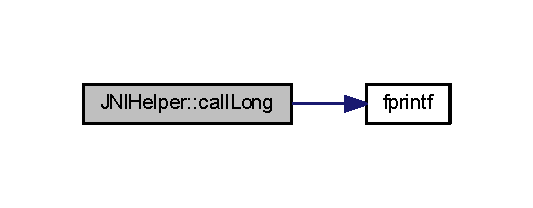
\includegraphics[width=256pt]{class_j_n_i_helper_a0c2378b0f3447af66038ae9f6dea1000_cgraph}
\end{center}
\end{figure}


\hypertarget{class_j_n_i_helper_ac6fc439bd0a306c475cc1392ff586951}{\index{J\-N\-I\-Helper@{J\-N\-I\-Helper}!call\-Object@{call\-Object}}
\index{call\-Object@{call\-Object}!JNIHelper@{J\-N\-I\-Helper}}
\subsubsection[{call\-Object}]{\setlength{\rightskip}{0pt plus 5cm}jobject J\-N\-I\-Helper\-::call\-Object (
\begin{DoxyParamCaption}
\item[{J\-N\-I\-Env $\ast$}]{jenv, }
\item[{jobject}]{instance, }
\item[{char $\ast$}]{method\-Name, }
\item[{char $\ast$}]{method\-Signature, }
\item[{}]{...}
\end{DoxyParamCaption}
)\hspace{0.3cm}{\ttfamily [static]}}}\label{class_j_n_i_helper_ac6fc439bd0a306c475cc1392ff586951}


Here is the call graph for this function\-:
\nopagebreak
\begin{figure}[H]
\begin{center}
\leavevmode
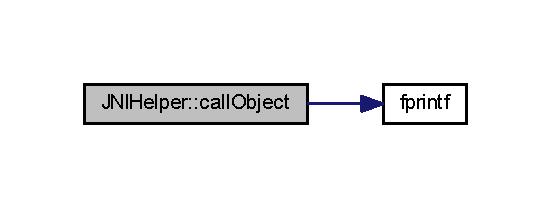
\includegraphics[width=264pt]{class_j_n_i_helper_ac6fc439bd0a306c475cc1392ff586951_cgraph}
\end{center}
\end{figure}


\hypertarget{class_j_n_i_helper_adff29cbca25d5f6787f675afcdc38871}{\index{J\-N\-I\-Helper@{J\-N\-I\-Helper}!call\-Void@{call\-Void}}
\index{call\-Void@{call\-Void}!JNIHelper@{J\-N\-I\-Helper}}
\subsubsection[{call\-Void}]{\setlength{\rightskip}{0pt plus 5cm}void J\-N\-I\-Helper\-::call\-Void (
\begin{DoxyParamCaption}
\item[{J\-N\-I\-Env $\ast$}]{jenv, }
\item[{jobject}]{instance, }
\item[{char $\ast$}]{method\-Name, }
\item[{char $\ast$}]{method\-Signature, }
\item[{}]{...}
\end{DoxyParamCaption}
)\hspace{0.3cm}{\ttfamily [static]}}}\label{class_j_n_i_helper_adff29cbca25d5f6787f675afcdc38871}


Here is the call graph for this function\-:
\nopagebreak
\begin{figure}[H]
\begin{center}
\leavevmode
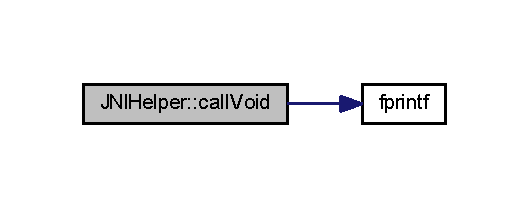
\includegraphics[width=254pt]{class_j_n_i_helper_adff29cbca25d5f6787f675afcdc38871_cgraph}
\end{center}
\end{figure}


\hypertarget{class_j_n_i_helper_a6d0240a89937c774bd5229944a54a544}{\index{J\-N\-I\-Helper@{J\-N\-I\-Helper}!create\-Instance@{create\-Instance}}
\index{create\-Instance@{create\-Instance}!JNIHelper@{J\-N\-I\-Helper}}
\subsubsection[{create\-Instance}]{\setlength{\rightskip}{0pt plus 5cm}jobject J\-N\-I\-Helper\-::create\-Instance (
\begin{DoxyParamCaption}
\item[{J\-N\-I\-Env $\ast$}]{jenv, }
\item[{char $\ast$}]{class\-Name, }
\item[{char $\ast$}]{signature, }
\item[{}]{...}
\end{DoxyParamCaption}
)\hspace{0.3cm}{\ttfamily [static]}}}\label{class_j_n_i_helper_a6d0240a89937c774bd5229944a54a544}


Here is the call graph for this function\-:
\nopagebreak
\begin{figure}[H]
\begin{center}
\leavevmode
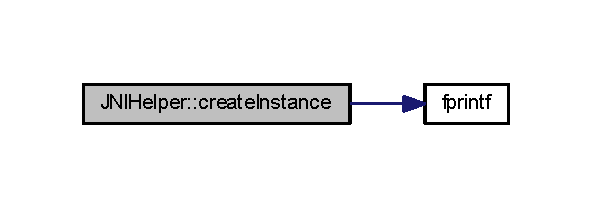
\includegraphics[width=284pt]{class_j_n_i_helper_a6d0240a89937c774bd5229944a54a544_cgraph}
\end{center}
\end{figure}




Here is the caller graph for this function\-:
\nopagebreak
\begin{figure}[H]
\begin{center}
\leavevmode
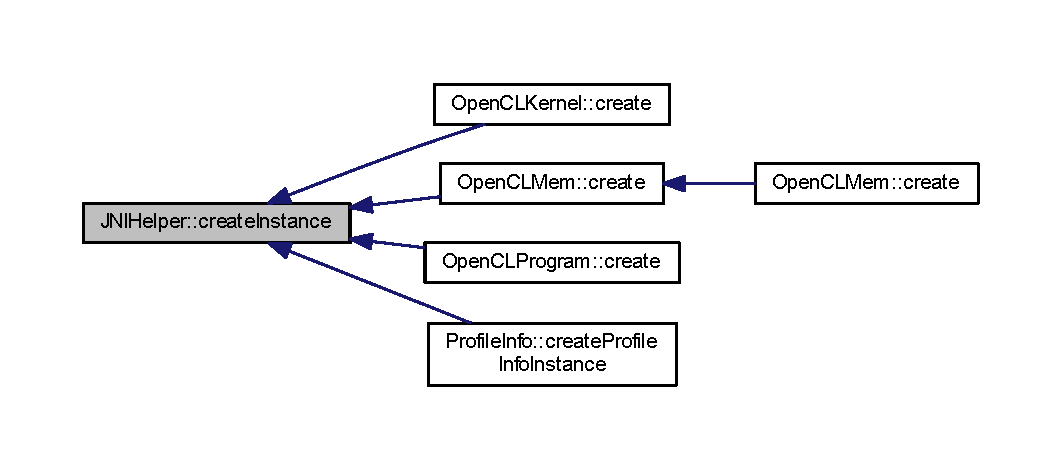
\includegraphics[width=350pt]{class_j_n_i_helper_a6d0240a89937c774bd5229944a54a544_icgraph}
\end{center}
\end{figure}


\hypertarget{class_j_n_i_helper_ad389729ad0900ed6f3ccc7a105e42c9a}{\index{J\-N\-I\-Helper@{J\-N\-I\-Helper}!get\-Field@{get\-Field}}
\index{get\-Field@{get\-Field}!JNIHelper@{J\-N\-I\-Helper}}
\subsubsection[{get\-Field}]{\setlength{\rightskip}{0pt plus 5cm}static void J\-N\-I\-Helper\-::get\-Field (
\begin{DoxyParamCaption}
\item[{J\-N\-I\-Env $\ast$}]{jenv, }
\item[{jobject}]{instance, }
\item[{jfield\-I\-D}]{field\-Id, }
\item[{jint $\ast$}]{value}
\end{DoxyParamCaption}
)\hspace{0.3cm}{\ttfamily [inline]}, {\ttfamily [static]}, {\ttfamily [private]}}}\label{class_j_n_i_helper_ad389729ad0900ed6f3ccc7a105e42c9a}


Here is the caller graph for this function\-:
\nopagebreak
\begin{figure}[H]
\begin{center}
\leavevmode
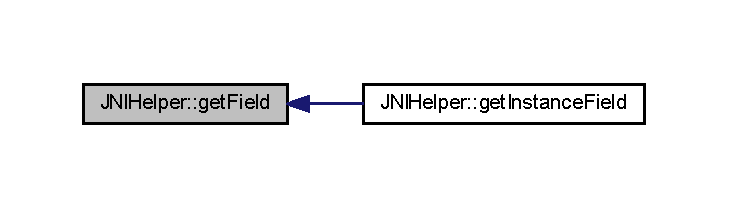
\includegraphics[width=350pt]{class_j_n_i_helper_ad389729ad0900ed6f3ccc7a105e42c9a_icgraph}
\end{center}
\end{figure}


\hypertarget{class_j_n_i_helper_aca90dfc2fcb39564f82a66cf01a8d4f6}{\index{J\-N\-I\-Helper@{J\-N\-I\-Helper}!get\-Field@{get\-Field}}
\index{get\-Field@{get\-Field}!JNIHelper@{J\-N\-I\-Helper}}
\subsubsection[{get\-Field}]{\setlength{\rightskip}{0pt plus 5cm}static void J\-N\-I\-Helper\-::get\-Field (
\begin{DoxyParamCaption}
\item[{J\-N\-I\-Env $\ast$}]{jenv, }
\item[{jobject}]{instance, }
\item[{jfield\-I\-D}]{field\-Id, }
\item[{jfloat $\ast$}]{value}
\end{DoxyParamCaption}
)\hspace{0.3cm}{\ttfamily [inline]}, {\ttfamily [static]}, {\ttfamily [private]}}}\label{class_j_n_i_helper_aca90dfc2fcb39564f82a66cf01a8d4f6}
\hypertarget{class_j_n_i_helper_a39cebd8486f32528314d28ecb1f709ca}{\index{J\-N\-I\-Helper@{J\-N\-I\-Helper}!get\-Field@{get\-Field}}
\index{get\-Field@{get\-Field}!JNIHelper@{J\-N\-I\-Helper}}
\subsubsection[{get\-Field}]{\setlength{\rightskip}{0pt plus 5cm}static void J\-N\-I\-Helper\-::get\-Field (
\begin{DoxyParamCaption}
\item[{J\-N\-I\-Env $\ast$}]{jenv, }
\item[{jobject}]{instance, }
\item[{jfield\-I\-D}]{field\-Id, }
\item[{jdouble $\ast$}]{value}
\end{DoxyParamCaption}
)\hspace{0.3cm}{\ttfamily [inline]}, {\ttfamily [static]}, {\ttfamily [private]}}}\label{class_j_n_i_helper_a39cebd8486f32528314d28ecb1f709ca}
\hypertarget{class_j_n_i_helper_a232126b247a62164c157494aaa7e8486}{\index{J\-N\-I\-Helper@{J\-N\-I\-Helper}!get\-Field@{get\-Field}}
\index{get\-Field@{get\-Field}!JNIHelper@{J\-N\-I\-Helper}}
\subsubsection[{get\-Field}]{\setlength{\rightskip}{0pt plus 5cm}static void J\-N\-I\-Helper\-::get\-Field (
\begin{DoxyParamCaption}
\item[{J\-N\-I\-Env $\ast$}]{jenv, }
\item[{jobject}]{instance, }
\item[{jfield\-I\-D}]{field\-Id, }
\item[{jshort $\ast$}]{value}
\end{DoxyParamCaption}
)\hspace{0.3cm}{\ttfamily [inline]}, {\ttfamily [static]}, {\ttfamily [private]}}}\label{class_j_n_i_helper_a232126b247a62164c157494aaa7e8486}
\hypertarget{class_j_n_i_helper_ab2641ea86b0b292f9bd8861b60a97b21}{\index{J\-N\-I\-Helper@{J\-N\-I\-Helper}!get\-Field@{get\-Field}}
\index{get\-Field@{get\-Field}!JNIHelper@{J\-N\-I\-Helper}}
\subsubsection[{get\-Field}]{\setlength{\rightskip}{0pt plus 5cm}static void J\-N\-I\-Helper\-::get\-Field (
\begin{DoxyParamCaption}
\item[{J\-N\-I\-Env $\ast$}]{jenv, }
\item[{jobject}]{instance, }
\item[{jfield\-I\-D}]{field\-Id, }
\item[{jlong $\ast$}]{value}
\end{DoxyParamCaption}
)\hspace{0.3cm}{\ttfamily [inline]}, {\ttfamily [static]}, {\ttfamily [private]}}}\label{class_j_n_i_helper_ab2641ea86b0b292f9bd8861b60a97b21}
\hypertarget{class_j_n_i_helper_a0096170be9f8685372dbf24ef35401a5}{\index{J\-N\-I\-Helper@{J\-N\-I\-Helper}!get\-Field@{get\-Field}}
\index{get\-Field@{get\-Field}!JNIHelper@{J\-N\-I\-Helper}}
\subsubsection[{get\-Field}]{\setlength{\rightskip}{0pt plus 5cm}static void J\-N\-I\-Helper\-::get\-Field (
\begin{DoxyParamCaption}
\item[{J\-N\-I\-Env $\ast$}]{jenv, }
\item[{jobject}]{instance, }
\item[{jfield\-I\-D}]{field\-Id, }
\item[{jobject $\ast$}]{value}
\end{DoxyParamCaption}
)\hspace{0.3cm}{\ttfamily [inline]}, {\ttfamily [static]}, {\ttfamily [private]}}}\label{class_j_n_i_helper_a0096170be9f8685372dbf24ef35401a5}
\hypertarget{class_j_n_i_helper_aec536897478d45cb8fea5f7396697eaa}{\index{J\-N\-I\-Helper@{J\-N\-I\-Helper}!get\-Field@{get\-Field}}
\index{get\-Field@{get\-Field}!JNIHelper@{J\-N\-I\-Helper}}
\subsubsection[{get\-Field}]{\setlength{\rightskip}{0pt plus 5cm}static void J\-N\-I\-Helper\-::get\-Field (
\begin{DoxyParamCaption}
\item[{J\-N\-I\-Env $\ast$}]{jenv, }
\item[{jobject}]{instance, }
\item[{jfield\-I\-D}]{field\-Id, }
\item[{jboolean $\ast$}]{value}
\end{DoxyParamCaption}
)\hspace{0.3cm}{\ttfamily [inline]}, {\ttfamily [static]}, {\ttfamily [private]}}}\label{class_j_n_i_helper_aec536897478d45cb8fea5f7396697eaa}
\hypertarget{class_j_n_i_helper_adc97179237bf9d5b36d06663c6bbc074}{\index{J\-N\-I\-Helper@{J\-N\-I\-Helper}!Get\-Field\-I\-D@{Get\-Field\-I\-D}}
\index{Get\-Field\-I\-D@{Get\-Field\-I\-D}!JNIHelper@{J\-N\-I\-Helper}}
\subsubsection[{Get\-Field\-I\-D}]{\setlength{\rightskip}{0pt plus 5cm}static jfield\-I\-D J\-N\-I\-Helper\-::\-Get\-Field\-I\-D (
\begin{DoxyParamCaption}
\item[{J\-N\-I\-Env $\ast$}]{jenv, }
\item[{jclass}]{c, }
\item[{const char $\ast$}]{name, }
\item[{const char $\ast$}]{type}
\end{DoxyParamCaption}
)\hspace{0.3cm}{\ttfamily [inline]}, {\ttfamily [static]}}}\label{class_j_n_i_helper_adc97179237bf9d5b36d06663c6bbc074}


Here is the call graph for this function\-:
\nopagebreak
\begin{figure}[H]
\begin{center}
\leavevmode
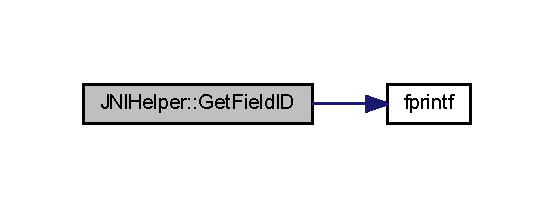
\includegraphics[width=266pt]{class_j_n_i_helper_adc97179237bf9d5b36d06663c6bbc074_cgraph}
\end{center}
\end{figure}




Here is the caller graph for this function\-:
\nopagebreak
\begin{figure}[H]
\begin{center}
\leavevmode
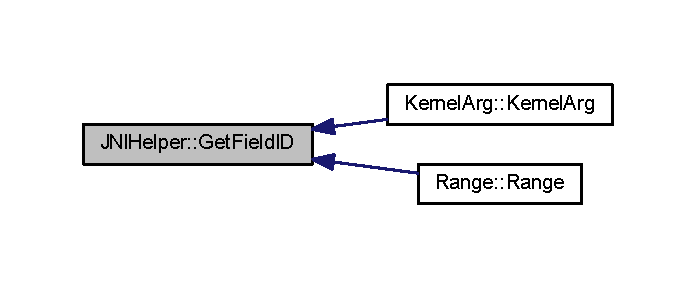
\includegraphics[width=334pt]{class_j_n_i_helper_adc97179237bf9d5b36d06663c6bbc074_icgraph}
\end{center}
\end{figure}


\hypertarget{class_j_n_i_helper_a1c640a98f51b1ace46bd99c8c1a75557}{\index{J\-N\-I\-Helper@{J\-N\-I\-Helper}!get\-Instance\-Field@{get\-Instance\-Field}}
\index{get\-Instance\-Field@{get\-Instance\-Field}!JNIHelper@{J\-N\-I\-Helper}}
\subsubsection[{get\-Instance\-Field}]{\setlength{\rightskip}{0pt plus 5cm}template$<$typename j\-T $>$ static j\-T J\-N\-I\-Helper\-::get\-Instance\-Field (
\begin{DoxyParamCaption}
\item[{J\-N\-I\-Env $\ast$}]{jenv, }
\item[{jobject}]{instance, }
\item[{const char $\ast$}]{field\-Name}
\end{DoxyParamCaption}
)\hspace{0.3cm}{\ttfamily [inline]}, {\ttfamily [static]}}}\label{class_j_n_i_helper_a1c640a98f51b1ace46bd99c8c1a75557}


Here is the call graph for this function\-:
\nopagebreak
\begin{figure}[H]
\begin{center}
\leavevmode
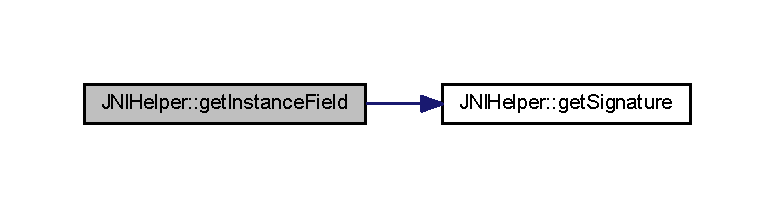
\includegraphics[width=350pt]{class_j_n_i_helper_a1c640a98f51b1ace46bd99c8c1a75557_cgraph}
\end{center}
\end{figure}


\hypertarget{class_j_n_i_helper_a1840235841c1159432d86a7a545564bd}{\index{J\-N\-I\-Helper@{J\-N\-I\-Helper}!get\-Instance\-Field@{get\-Instance\-Field}}
\index{get\-Instance\-Field@{get\-Instance\-Field}!JNIHelper@{J\-N\-I\-Helper}}
\subsubsection[{get\-Instance\-Field}]{\setlength{\rightskip}{0pt plus 5cm}template$<$typename j\-T $>$ static j\-T J\-N\-I\-Helper\-::get\-Instance\-Field (
\begin{DoxyParamCaption}
\item[{J\-N\-I\-Env $\ast$}]{jenv, }
\item[{jobject}]{instance, }
\item[{const char $\ast$}]{field\-Name, }
\item[{const char $\ast$}]{signature}
\end{DoxyParamCaption}
)\hspace{0.3cm}{\ttfamily [inline]}, {\ttfamily [static]}}}\label{class_j_n_i_helper_a1840235841c1159432d86a7a545564bd}


Here is the call graph for this function\-:
\nopagebreak
\begin{figure}[H]
\begin{center}
\leavevmode
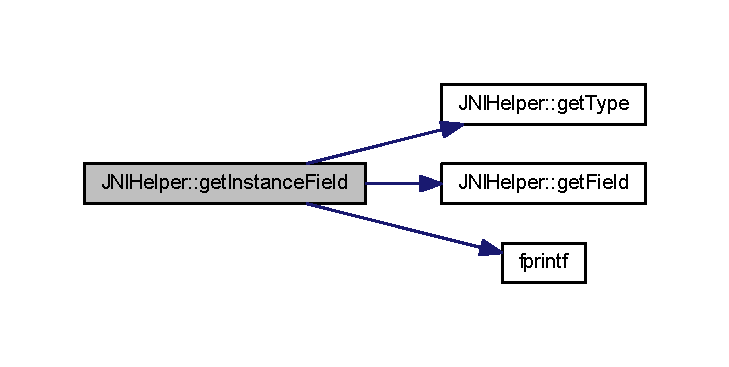
\includegraphics[width=350pt]{class_j_n_i_helper_a1840235841c1159432d86a7a545564bd_cgraph}
\end{center}
\end{figure}


\hypertarget{class_j_n_i_helper_ac4ea33f6aba560ceea078bf3ef2cc90f}{\index{J\-N\-I\-Helper@{J\-N\-I\-Helper}!get\-Signature@{get\-Signature}}
\index{get\-Signature@{get\-Signature}!JNIHelper@{J\-N\-I\-Helper}}
\subsubsection[{get\-Signature}]{\setlength{\rightskip}{0pt plus 5cm}static const char$\ast$ J\-N\-I\-Helper\-::get\-Signature (
\begin{DoxyParamCaption}
\item[{jint}]{value}
\end{DoxyParamCaption}
)\hspace{0.3cm}{\ttfamily [inline]}, {\ttfamily [static]}, {\ttfamily [private]}}}\label{class_j_n_i_helper_ac4ea33f6aba560ceea078bf3ef2cc90f}


Here is the caller graph for this function\-:
\nopagebreak
\begin{figure}[H]
\begin{center}
\leavevmode
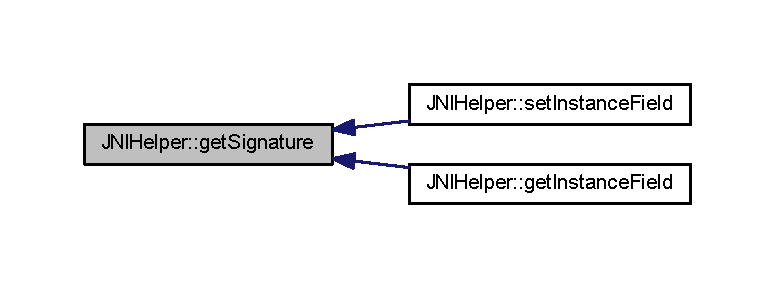
\includegraphics[width=350pt]{class_j_n_i_helper_ac4ea33f6aba560ceea078bf3ef2cc90f_icgraph}
\end{center}
\end{figure}


\hypertarget{class_j_n_i_helper_a89c38cc5a13ff61937e9d1f3fc8addea}{\index{J\-N\-I\-Helper@{J\-N\-I\-Helper}!get\-Signature@{get\-Signature}}
\index{get\-Signature@{get\-Signature}!JNIHelper@{J\-N\-I\-Helper}}
\subsubsection[{get\-Signature}]{\setlength{\rightskip}{0pt plus 5cm}static const char$\ast$ J\-N\-I\-Helper\-::get\-Signature (
\begin{DoxyParamCaption}
\item[{jfloat}]{value}
\end{DoxyParamCaption}
)\hspace{0.3cm}{\ttfamily [inline]}, {\ttfamily [static]}, {\ttfamily [private]}}}\label{class_j_n_i_helper_a89c38cc5a13ff61937e9d1f3fc8addea}
\hypertarget{class_j_n_i_helper_a9ed865d10a616b55449cf7f3e4620b2f}{\index{J\-N\-I\-Helper@{J\-N\-I\-Helper}!get\-Signature@{get\-Signature}}
\index{get\-Signature@{get\-Signature}!JNIHelper@{J\-N\-I\-Helper}}
\subsubsection[{get\-Signature}]{\setlength{\rightskip}{0pt plus 5cm}static const char$\ast$ J\-N\-I\-Helper\-::get\-Signature (
\begin{DoxyParamCaption}
\item[{jdouble}]{value}
\end{DoxyParamCaption}
)\hspace{0.3cm}{\ttfamily [inline]}, {\ttfamily [static]}, {\ttfamily [private]}}}\label{class_j_n_i_helper_a9ed865d10a616b55449cf7f3e4620b2f}
\hypertarget{class_j_n_i_helper_a5949905b5e2730a12829398dba7032d2}{\index{J\-N\-I\-Helper@{J\-N\-I\-Helper}!get\-Signature@{get\-Signature}}
\index{get\-Signature@{get\-Signature}!JNIHelper@{J\-N\-I\-Helper}}
\subsubsection[{get\-Signature}]{\setlength{\rightskip}{0pt plus 5cm}static const char$\ast$ J\-N\-I\-Helper\-::get\-Signature (
\begin{DoxyParamCaption}
\item[{jshort}]{value}
\end{DoxyParamCaption}
)\hspace{0.3cm}{\ttfamily [inline]}, {\ttfamily [static]}, {\ttfamily [private]}}}\label{class_j_n_i_helper_a5949905b5e2730a12829398dba7032d2}
\hypertarget{class_j_n_i_helper_aa9e066ff111d23fcbcab00cf03d53792}{\index{J\-N\-I\-Helper@{J\-N\-I\-Helper}!get\-Signature@{get\-Signature}}
\index{get\-Signature@{get\-Signature}!JNIHelper@{J\-N\-I\-Helper}}
\subsubsection[{get\-Signature}]{\setlength{\rightskip}{0pt plus 5cm}static const char$\ast$ J\-N\-I\-Helper\-::get\-Signature (
\begin{DoxyParamCaption}
\item[{jlong}]{value}
\end{DoxyParamCaption}
)\hspace{0.3cm}{\ttfamily [inline]}, {\ttfamily [static]}, {\ttfamily [private]}}}\label{class_j_n_i_helper_aa9e066ff111d23fcbcab00cf03d53792}
\hypertarget{class_j_n_i_helper_a0e9db8bd345fcce18ff7cee46c23b8a1}{\index{J\-N\-I\-Helper@{J\-N\-I\-Helper}!get\-Signature@{get\-Signature}}
\index{get\-Signature@{get\-Signature}!JNIHelper@{J\-N\-I\-Helper}}
\subsubsection[{get\-Signature}]{\setlength{\rightskip}{0pt plus 5cm}static const char$\ast$ J\-N\-I\-Helper\-::get\-Signature (
\begin{DoxyParamCaption}
\item[{jboolean}]{value}
\end{DoxyParamCaption}
)\hspace{0.3cm}{\ttfamily [inline]}, {\ttfamily [static]}, {\ttfamily [private]}}}\label{class_j_n_i_helper_a0e9db8bd345fcce18ff7cee46c23b8a1}
\hypertarget{class_j_n_i_helper_a62620661bbb5a7eb1c38cedccb2d9066}{\index{J\-N\-I\-Helper@{J\-N\-I\-Helper}!get\-Static\-Field\-Object@{get\-Static\-Field\-Object}}
\index{get\-Static\-Field\-Object@{get\-Static\-Field\-Object}!JNIHelper@{J\-N\-I\-Helper}}
\subsubsection[{get\-Static\-Field\-Object}]{\setlength{\rightskip}{0pt plus 5cm}jobject J\-N\-I\-Helper\-::get\-Static\-Field\-Object (
\begin{DoxyParamCaption}
\item[{J\-N\-I\-Env $\ast$}]{jenv, }
\item[{char $\ast$}]{class\-Name, }
\item[{char $\ast$}]{field\-Name, }
\item[{char $\ast$}]{signature}
\end{DoxyParamCaption}
)\hspace{0.3cm}{\ttfamily [static]}}}\label{class_j_n_i_helper_a62620661bbb5a7eb1c38cedccb2d9066}


Here is the call graph for this function\-:
\nopagebreak
\begin{figure}[H]
\begin{center}
\leavevmode
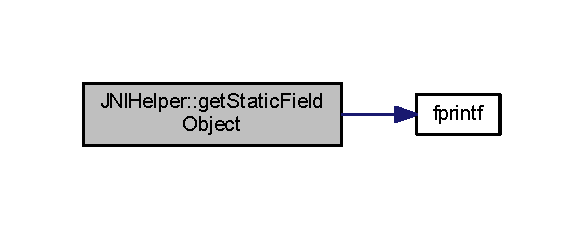
\includegraphics[width=280pt]{class_j_n_i_helper_a62620661bbb5a7eb1c38cedccb2d9066_cgraph}
\end{center}
\end{figure}


\hypertarget{class_j_n_i_helper_a6934bf9b61e058225184032cfc49bf08}{\index{J\-N\-I\-Helper@{J\-N\-I\-Helper}!get\-Type@{get\-Type}}
\index{get\-Type@{get\-Type}!JNIHelper@{J\-N\-I\-Helper}}
\subsubsection[{get\-Type}]{\setlength{\rightskip}{0pt plus 5cm}static std\-::string J\-N\-I\-Helper\-::get\-Type (
\begin{DoxyParamCaption}
\item[{jint}]{value}
\end{DoxyParamCaption}
)\hspace{0.3cm}{\ttfamily [inline]}, {\ttfamily [static]}}}\label{class_j_n_i_helper_a6934bf9b61e058225184032cfc49bf08}


Here is the caller graph for this function\-:
\nopagebreak
\begin{figure}[H]
\begin{center}
\leavevmode
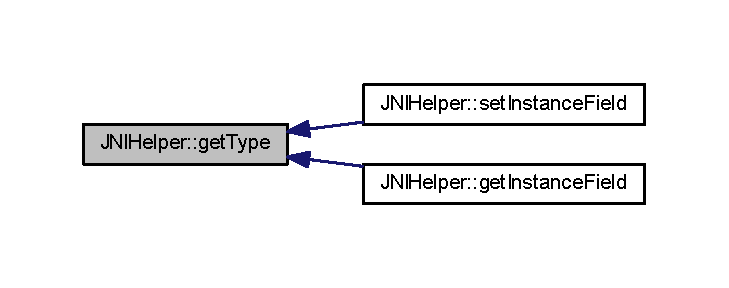
\includegraphics[width=350pt]{class_j_n_i_helper_a6934bf9b61e058225184032cfc49bf08_icgraph}
\end{center}
\end{figure}


\hypertarget{class_j_n_i_helper_a3d4a3261b07e28a398bd99d59deb4160}{\index{J\-N\-I\-Helper@{J\-N\-I\-Helper}!get\-Type@{get\-Type}}
\index{get\-Type@{get\-Type}!JNIHelper@{J\-N\-I\-Helper}}
\subsubsection[{get\-Type}]{\setlength{\rightskip}{0pt plus 5cm}static std\-::string J\-N\-I\-Helper\-::get\-Type (
\begin{DoxyParamCaption}
\item[{jfloat}]{value}
\end{DoxyParamCaption}
)\hspace{0.3cm}{\ttfamily [inline]}, {\ttfamily [static]}}}\label{class_j_n_i_helper_a3d4a3261b07e28a398bd99d59deb4160}
\hypertarget{class_j_n_i_helper_ad781e04f8719bcfa2a33868867a2a4b5}{\index{J\-N\-I\-Helper@{J\-N\-I\-Helper}!get\-Type@{get\-Type}}
\index{get\-Type@{get\-Type}!JNIHelper@{J\-N\-I\-Helper}}
\subsubsection[{get\-Type}]{\setlength{\rightskip}{0pt plus 5cm}static std\-::string J\-N\-I\-Helper\-::get\-Type (
\begin{DoxyParamCaption}
\item[{jdouble}]{value}
\end{DoxyParamCaption}
)\hspace{0.3cm}{\ttfamily [inline]}, {\ttfamily [static]}}}\label{class_j_n_i_helper_ad781e04f8719bcfa2a33868867a2a4b5}
\hypertarget{class_j_n_i_helper_a206d661817dd7011bf611e2c52160d59}{\index{J\-N\-I\-Helper@{J\-N\-I\-Helper}!get\-Type@{get\-Type}}
\index{get\-Type@{get\-Type}!JNIHelper@{J\-N\-I\-Helper}}
\subsubsection[{get\-Type}]{\setlength{\rightskip}{0pt plus 5cm}static std\-::string J\-N\-I\-Helper\-::get\-Type (
\begin{DoxyParamCaption}
\item[{jshort}]{value}
\end{DoxyParamCaption}
)\hspace{0.3cm}{\ttfamily [inline]}, {\ttfamily [static]}}}\label{class_j_n_i_helper_a206d661817dd7011bf611e2c52160d59}
\hypertarget{class_j_n_i_helper_a2a101aa6ff2af7a1ca5d80be913ea46a}{\index{J\-N\-I\-Helper@{J\-N\-I\-Helper}!get\-Type@{get\-Type}}
\index{get\-Type@{get\-Type}!JNIHelper@{J\-N\-I\-Helper}}
\subsubsection[{get\-Type}]{\setlength{\rightskip}{0pt plus 5cm}static std\-::string J\-N\-I\-Helper\-::get\-Type (
\begin{DoxyParamCaption}
\item[{jlong}]{value}
\end{DoxyParamCaption}
)\hspace{0.3cm}{\ttfamily [inline]}, {\ttfamily [static]}}}\label{class_j_n_i_helper_a2a101aa6ff2af7a1ca5d80be913ea46a}
\hypertarget{class_j_n_i_helper_a89e129b46a8d1cdee4e9ac5840d42f30}{\index{J\-N\-I\-Helper@{J\-N\-I\-Helper}!get\-Type@{get\-Type}}
\index{get\-Type@{get\-Type}!JNIHelper@{J\-N\-I\-Helper}}
\subsubsection[{get\-Type}]{\setlength{\rightskip}{0pt plus 5cm}static std\-::string J\-N\-I\-Helper\-::get\-Type (
\begin{DoxyParamCaption}
\item[{jobject}]{value}
\end{DoxyParamCaption}
)\hspace{0.3cm}{\ttfamily [inline]}, {\ttfamily [static]}}}\label{class_j_n_i_helper_a89e129b46a8d1cdee4e9ac5840d42f30}
\hypertarget{class_j_n_i_helper_a777e896380d762f15c61c051907fa98d}{\index{J\-N\-I\-Helper@{J\-N\-I\-Helper}!get\-Type@{get\-Type}}
\index{get\-Type@{get\-Type}!JNIHelper@{J\-N\-I\-Helper}}
\subsubsection[{get\-Type}]{\setlength{\rightskip}{0pt plus 5cm}static std\-::string J\-N\-I\-Helper\-::get\-Type (
\begin{DoxyParamCaption}
\item[{jboolean}]{value}
\end{DoxyParamCaption}
)\hspace{0.3cm}{\ttfamily [inline]}, {\ttfamily [static]}}}\label{class_j_n_i_helper_a777e896380d762f15c61c051907fa98d}
\hypertarget{class_j_n_i_helper_a8265ea28e2311aac6a66a2b794b4a8fe}{\index{J\-N\-I\-Helper@{J\-N\-I\-Helper}!set\-Field@{set\-Field}}
\index{set\-Field@{set\-Field}!JNIHelper@{J\-N\-I\-Helper}}
\subsubsection[{set\-Field}]{\setlength{\rightskip}{0pt plus 5cm}static void J\-N\-I\-Helper\-::set\-Field (
\begin{DoxyParamCaption}
\item[{J\-N\-I\-Env $\ast$}]{jenv, }
\item[{jobject}]{instance, }
\item[{jfield\-I\-D}]{field\-Id, }
\item[{jint $\ast$}]{value}
\end{DoxyParamCaption}
)\hspace{0.3cm}{\ttfamily [inline]}, {\ttfamily [static]}, {\ttfamily [private]}}}\label{class_j_n_i_helper_a8265ea28e2311aac6a66a2b794b4a8fe}


Here is the caller graph for this function\-:
\nopagebreak
\begin{figure}[H]
\begin{center}
\leavevmode
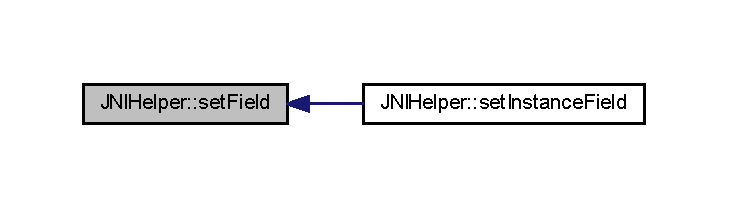
\includegraphics[width=350pt]{class_j_n_i_helper_a8265ea28e2311aac6a66a2b794b4a8fe_icgraph}
\end{center}
\end{figure}


\hypertarget{class_j_n_i_helper_a6a24cbc36c6c00c8062735b872c9ddb5}{\index{J\-N\-I\-Helper@{J\-N\-I\-Helper}!set\-Field@{set\-Field}}
\index{set\-Field@{set\-Field}!JNIHelper@{J\-N\-I\-Helper}}
\subsubsection[{set\-Field}]{\setlength{\rightskip}{0pt plus 5cm}static void J\-N\-I\-Helper\-::set\-Field (
\begin{DoxyParamCaption}
\item[{J\-N\-I\-Env $\ast$}]{jenv, }
\item[{jobject}]{instance, }
\item[{jfield\-I\-D}]{field\-Id, }
\item[{jfloat $\ast$}]{value}
\end{DoxyParamCaption}
)\hspace{0.3cm}{\ttfamily [inline]}, {\ttfamily [static]}, {\ttfamily [private]}}}\label{class_j_n_i_helper_a6a24cbc36c6c00c8062735b872c9ddb5}
\hypertarget{class_j_n_i_helper_a91745290d3dbba0bc0e899a2e4cbb0b3}{\index{J\-N\-I\-Helper@{J\-N\-I\-Helper}!set\-Field@{set\-Field}}
\index{set\-Field@{set\-Field}!JNIHelper@{J\-N\-I\-Helper}}
\subsubsection[{set\-Field}]{\setlength{\rightskip}{0pt plus 5cm}static void J\-N\-I\-Helper\-::set\-Field (
\begin{DoxyParamCaption}
\item[{J\-N\-I\-Env $\ast$}]{jenv, }
\item[{jobject}]{instance, }
\item[{jfield\-I\-D}]{field\-Id, }
\item[{jdouble $\ast$}]{value}
\end{DoxyParamCaption}
)\hspace{0.3cm}{\ttfamily [inline]}, {\ttfamily [static]}, {\ttfamily [private]}}}\label{class_j_n_i_helper_a91745290d3dbba0bc0e899a2e4cbb0b3}
\hypertarget{class_j_n_i_helper_a707937851d5e36013feb79dd29e79978}{\index{J\-N\-I\-Helper@{J\-N\-I\-Helper}!set\-Field@{set\-Field}}
\index{set\-Field@{set\-Field}!JNIHelper@{J\-N\-I\-Helper}}
\subsubsection[{set\-Field}]{\setlength{\rightskip}{0pt plus 5cm}static void J\-N\-I\-Helper\-::set\-Field (
\begin{DoxyParamCaption}
\item[{J\-N\-I\-Env $\ast$}]{jenv, }
\item[{jobject}]{instance, }
\item[{jfield\-I\-D}]{field\-Id, }
\item[{jshort $\ast$}]{value}
\end{DoxyParamCaption}
)\hspace{0.3cm}{\ttfamily [inline]}, {\ttfamily [static]}, {\ttfamily [private]}}}\label{class_j_n_i_helper_a707937851d5e36013feb79dd29e79978}
\hypertarget{class_j_n_i_helper_ae1272f3e616aed8c1ba6ba775e73dc7d}{\index{J\-N\-I\-Helper@{J\-N\-I\-Helper}!set\-Field@{set\-Field}}
\index{set\-Field@{set\-Field}!JNIHelper@{J\-N\-I\-Helper}}
\subsubsection[{set\-Field}]{\setlength{\rightskip}{0pt plus 5cm}static void J\-N\-I\-Helper\-::set\-Field (
\begin{DoxyParamCaption}
\item[{J\-N\-I\-Env $\ast$}]{jenv, }
\item[{jobject}]{instance, }
\item[{jfield\-I\-D}]{field\-Id, }
\item[{jlong $\ast$}]{value}
\end{DoxyParamCaption}
)\hspace{0.3cm}{\ttfamily [inline]}, {\ttfamily [static]}, {\ttfamily [private]}}}\label{class_j_n_i_helper_ae1272f3e616aed8c1ba6ba775e73dc7d}
\hypertarget{class_j_n_i_helper_a135376558da387f45f147c1d32cd5c21}{\index{J\-N\-I\-Helper@{J\-N\-I\-Helper}!set\-Field@{set\-Field}}
\index{set\-Field@{set\-Field}!JNIHelper@{J\-N\-I\-Helper}}
\subsubsection[{set\-Field}]{\setlength{\rightskip}{0pt plus 5cm}static void J\-N\-I\-Helper\-::set\-Field (
\begin{DoxyParamCaption}
\item[{J\-N\-I\-Env $\ast$}]{jenv, }
\item[{jobject}]{instance, }
\item[{jfield\-I\-D}]{field\-Id, }
\item[{jobject $\ast$}]{value}
\end{DoxyParamCaption}
)\hspace{0.3cm}{\ttfamily [inline]}, {\ttfamily [static]}, {\ttfamily [private]}}}\label{class_j_n_i_helper_a135376558da387f45f147c1d32cd5c21}
\hypertarget{class_j_n_i_helper_a53481dbf082667c76aff43e32e90bdf6}{\index{J\-N\-I\-Helper@{J\-N\-I\-Helper}!set\-Field@{set\-Field}}
\index{set\-Field@{set\-Field}!JNIHelper@{J\-N\-I\-Helper}}
\subsubsection[{set\-Field}]{\setlength{\rightskip}{0pt plus 5cm}static void J\-N\-I\-Helper\-::set\-Field (
\begin{DoxyParamCaption}
\item[{J\-N\-I\-Env $\ast$}]{jenv, }
\item[{jobject}]{instance, }
\item[{jfield\-I\-D}]{field\-Id, }
\item[{jboolean $\ast$}]{value}
\end{DoxyParamCaption}
)\hspace{0.3cm}{\ttfamily [inline]}, {\ttfamily [static]}, {\ttfamily [private]}}}\label{class_j_n_i_helper_a53481dbf082667c76aff43e32e90bdf6}
\hypertarget{class_j_n_i_helper_a950f746b15f97df78e3150de33c16422}{\index{J\-N\-I\-Helper@{J\-N\-I\-Helper}!set\-Instance\-Field@{set\-Instance\-Field}}
\index{set\-Instance\-Field@{set\-Instance\-Field}!JNIHelper@{J\-N\-I\-Helper}}
\subsubsection[{set\-Instance\-Field}]{\setlength{\rightskip}{0pt plus 5cm}template$<$typename j\-T $>$ static void J\-N\-I\-Helper\-::set\-Instance\-Field (
\begin{DoxyParamCaption}
\item[{J\-N\-I\-Env $\ast$}]{jenv, }
\item[{jobject}]{instance, }
\item[{const char $\ast$}]{field\-Name, }
\item[{j\-T}]{value}
\end{DoxyParamCaption}
)\hspace{0.3cm}{\ttfamily [inline]}, {\ttfamily [static]}}}\label{class_j_n_i_helper_a950f746b15f97df78e3150de33c16422}


Here is the call graph for this function\-:
\nopagebreak
\begin{figure}[H]
\begin{center}
\leavevmode
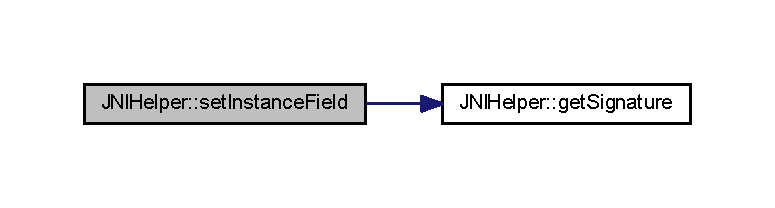
\includegraphics[width=350pt]{class_j_n_i_helper_a950f746b15f97df78e3150de33c16422_cgraph}
\end{center}
\end{figure}


\hypertarget{class_j_n_i_helper_aecce0e924d9c77e74e09220ba3112c87}{\index{J\-N\-I\-Helper@{J\-N\-I\-Helper}!set\-Instance\-Field@{set\-Instance\-Field}}
\index{set\-Instance\-Field@{set\-Instance\-Field}!JNIHelper@{J\-N\-I\-Helper}}
\subsubsection[{set\-Instance\-Field}]{\setlength{\rightskip}{0pt plus 5cm}template$<$typename j\-T $>$ static void J\-N\-I\-Helper\-::set\-Instance\-Field (
\begin{DoxyParamCaption}
\item[{J\-N\-I\-Env $\ast$}]{jenv, }
\item[{jobject}]{instance, }
\item[{const char $\ast$}]{field\-Name, }
\item[{const char $\ast$}]{signature, }
\item[{j\-T}]{value}
\end{DoxyParamCaption}
)\hspace{0.3cm}{\ttfamily [inline]}, {\ttfamily [static]}}}\label{class_j_n_i_helper_aecce0e924d9c77e74e09220ba3112c87}


Here is the call graph for this function\-:
\nopagebreak
\begin{figure}[H]
\begin{center}
\leavevmode
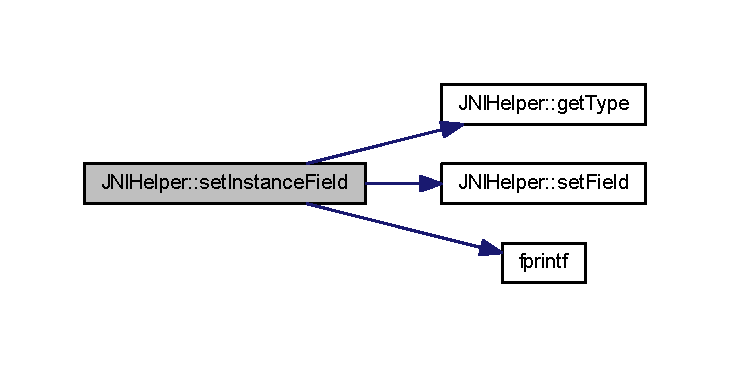
\includegraphics[width=350pt]{class_j_n_i_helper_aecce0e924d9c77e74e09220ba3112c87_cgraph}
\end{center}
\end{figure}




The documentation for this class was generated from the following files\-:\begin{DoxyCompactItemize}
\item 
src/cpp/\hyperlink{jni_helper_8h}{jni\-Helper.\-h}\item 
src/cpp/\hyperlink{jni_helper_8cpp}{jni\-Helper.\-cpp}\end{DoxyCompactItemize}

\hypertarget{class_kernel_arg}{\section{Kernel\-Arg Class Reference}
\label{class_kernel_arg}\index{Kernel\-Arg@{Kernel\-Arg}}
}


{\ttfamily \#include $<$Kernel\-Arg.\-h$>$}



Collaboration diagram for Kernel\-Arg\-:
\nopagebreak
\begin{figure}[H]
\begin{center}
\leavevmode
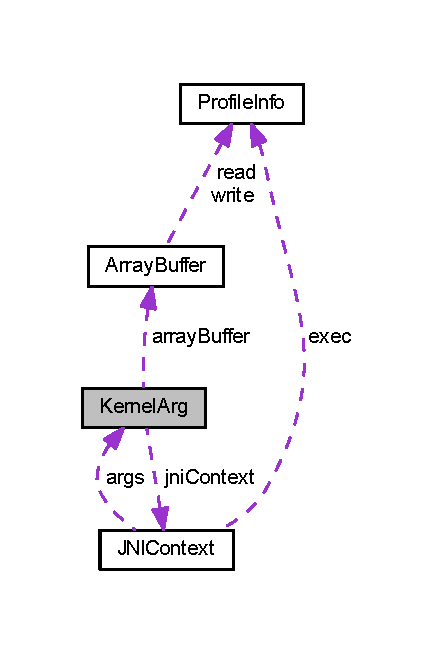
\includegraphics[width=210pt]{class_kernel_arg__coll__graph}
\end{center}
\end{figure}
\subsection*{Public Member Functions}
\begin{DoxyCompactItemize}
\item 
\hyperlink{class_kernel_arg_ae64310c9ca39693e96f97c78d2e484fa}{Kernel\-Arg} (J\-N\-I\-Env $\ast$\hyperlink{aparapi_8cpp_a31595c73e9a3750524b2ff61b5a14f96}{jenv}, \hyperlink{class_j_n_i_context}{J\-N\-I\-Context} $\ast$\hyperlink{class_kernel_arg_a5247a11aa8a301c025343b80ede7d9f5}{jni\-Context}, jobject \hyperlink{class_kernel_arg_a6c682f2814e39eca2a5bd66a056e69b5}{arg\-Obj})
\item 
\hyperlink{class_kernel_arg_acce352eb369167bfe41b7053fb13cc05}{$\sim$\-Kernel\-Arg} ()
\item 
void \hyperlink{class_kernel_arg_ab48f5be29c51a426b9b76353c593c47f}{unpin\-Abort} (J\-N\-I\-Env $\ast$\hyperlink{aparapi_8cpp_a31595c73e9a3750524b2ff61b5a14f96}{jenv})
\item 
void \hyperlink{class_kernel_arg_ac9b362583f7bfd45579728b64ef07c9a}{unpin\-Commit} (J\-N\-I\-Env $\ast$\hyperlink{aparapi_8cpp_a31595c73e9a3750524b2ff61b5a14f96}{jenv})
\item 
void \hyperlink{class_kernel_arg_ad3d62d6f3e6cc7891c0a871900dc7ee1}{unpin} (J\-N\-I\-Env $\ast$\hyperlink{aparapi_8cpp_a31595c73e9a3750524b2ff61b5a14f96}{jenv})
\item 
void \hyperlink{class_kernel_arg_a6fc2b16f01ddb5fba224d38fabc128cf}{pin} (J\-N\-I\-Env $\ast$\hyperlink{aparapi_8cpp_a31595c73e9a3750524b2ff61b5a14f96}{jenv})
\item 
int \hyperlink{class_kernel_arg_a5d1c17442e6f96aa1aeb834a82ed6950}{is\-Array} ()
\item 
int \hyperlink{class_kernel_arg_a164df3cf2ae35d7b53f5796e46c01fe5}{is\-Read\-By\-Kernel} ()
\item 
int \hyperlink{class_kernel_arg_aa1002b4a71aaa86b3089beee7f84d325}{is\-Mutable\-By\-Kernel} ()
\item 
int \hyperlink{class_kernel_arg_a14a83444c553bc8b8458223af8339e3d}{is\-Explicit} ()
\item 
int \hyperlink{class_kernel_arg_a4c7a7abe38cc18d254136b89ee817306}{uses\-Array\-Length} ()
\item 
int \hyperlink{class_kernel_arg_a080a2a1cae98156eec8dff6409b3c5f2}{is\-Explicit\-Write} ()
\item 
int \hyperlink{class_kernel_arg_ab8a775d67ecb9bf9c8ad4654fe7c3f58}{is\-Implicit} ()
\item 
int \hyperlink{class_kernel_arg_a11ed28ef2892d605343092d77570c859}{is\-Primitive} ()
\item 
int \hyperlink{class_kernel_arg_ae38da6f0073ce862e16c2f21ef451d0b}{is\-Global} ()
\item 
int \hyperlink{class_kernel_arg_a80c129f34138199a1d6495e509a769f1}{is\-Float} ()
\item 
int \hyperlink{class_kernel_arg_a92b487c069a5e65ba49d56ab867329a3}{is\-Long} ()
\item 
int \hyperlink{class_kernel_arg_adcf1efdd8a1c804db121c7f466472716}{is\-Int} ()
\item 
int \hyperlink{class_kernel_arg_ac8b08f0b2210d4217dac92f27389f330}{is\-Double} ()
\item 
int \hyperlink{class_kernel_arg_a6eea48cf98d46f8d50ee53a1edcc195f}{is\-Boolean} ()
\item 
int \hyperlink{class_kernel_arg_ac4905b9b405fc2a93d05127516d6777f}{is\-Byte} ()
\item 
int \hyperlink{class_kernel_arg_a0b9156ed4ddabff7c63b39973c4f81a2}{is\-Short} ()
\item 
int \hyperlink{class_kernel_arg_ab4e2866a831ea45934cec64566fb4816}{is\-Local} ()
\item 
int \hyperlink{class_kernel_arg_aae70fdc4496f4c2f3847dc01e3acf97d}{is\-Static} ()
\item 
int \hyperlink{class_kernel_arg_a266bef2508f3aa4c1f2e670b7658f05e}{is\-Constant} ()
\item 
int \hyperlink{class_kernel_arg_a49be011b2c8ee9f85d507521854fb4f8}{is\-Aparapi\-Buf} ()
\item 
int \hyperlink{class_kernel_arg_a8e5e4bf1b90efaf6a805028f831968da}{is\-Backed\-By\-Array} ()
\item 
int \hyperlink{class_kernel_arg_a789786a4bb65c3ac76299474ee371c87}{need\-To\-Enqueue\-Read} ()
\item 
int \hyperlink{class_kernel_arg_a42f6eead7b43c2e0839aae776c09bcb3}{need\-To\-Enqueue\-Write} ()
\item 
void \hyperlink{class_kernel_arg_a8d734fc1a5ebd7893a59e62cd58b8494}{sync\-Type} (J\-N\-I\-Env $\ast$\hyperlink{aparapi_8cpp_a31595c73e9a3750524b2ff61b5a14f96}{jenv})
\item 
void \hyperlink{class_kernel_arg_a9562b79167d156ca9902a885042d63ed}{sync\-Size\-In\-Bytes} (J\-N\-I\-Env $\ast$\hyperlink{aparapi_8cpp_a31595c73e9a3750524b2ff61b5a14f96}{jenv})
\item 
void \hyperlink{class_kernel_arg_a121239122f29829dd24a8971a207951b}{sync\-Java\-Array\-Length} (J\-N\-I\-Env $\ast$\hyperlink{aparapi_8cpp_a31595c73e9a3750524b2ff61b5a14f96}{jenv})
\item 
void \hyperlink{class_kernel_arg_ae5df1dec0f6ec684d58b2adf23dd1845}{clear\-Explicit\-Buffer\-Bit} (J\-N\-I\-Env $\ast$\hyperlink{aparapi_8cpp_a31595c73e9a3750524b2ff61b5a14f96}{jenv})
\item 
void \hyperlink{class_kernel_arg_a6a0caaeffc99a55b80361454dda5d091}{sync\-Value} (J\-N\-I\-Env $\ast$\hyperlink{aparapi_8cpp_a31595c73e9a3750524b2ff61b5a14f96}{jenv})
\item 
cl\-\_\-int \hyperlink{class_kernel_arg_a773fa9e962e4c5e72d2cc90f94b5a9c2}{set\-Local\-Buffer\-Arg} (J\-N\-I\-Env $\ast$\hyperlink{aparapi_8cpp_a31595c73e9a3750524b2ff61b5a14f96}{jenv}, int arg\-Idx, int \hyperlink{aparapi_8cpp_ab860a017c322839deee8d7bff5f0e180}{arg\-Pos}, bool verbose)
\item 
cl\-\_\-int \hyperlink{class_kernel_arg_aaeb024c19d0269f3a18076bb280c512c}{set\-Primitive\-Arg} (J\-N\-I\-Env $\ast$\hyperlink{aparapi_8cpp_a31595c73e9a3750524b2ff61b5a14f96}{jenv}, int arg\-Idx, int \hyperlink{aparapi_8cpp_ab860a017c322839deee8d7bff5f0e180}{arg\-Pos}, bool verbose)
\end{DoxyCompactItemize}
\subsection*{Public Attributes}
\begin{DoxyCompactItemize}
\item 
\hyperlink{class_j_n_i_context}{J\-N\-I\-Context} $\ast$ \hyperlink{class_kernel_arg_a5247a11aa8a301c025343b80ede7d9f5}{jni\-Context}
\item 
jobject \hyperlink{class_kernel_arg_a6c682f2814e39eca2a5bd66a056e69b5}{arg\-Obj}
\item 
jobject \hyperlink{class_kernel_arg_a34bc41a663249aca5caecbce438ce6a2}{java\-Arg}
\item 
char $\ast$ \hyperlink{class_kernel_arg_acbc4043bda1ccf9dafc93e7eaa7fb8e8}{name}
\item 
jint \hyperlink{class_kernel_arg_ab559d267fed499ad291ddd9b4596dd72}{type}
\item 
\hyperlink{class_array_buffer}{Array\-Buffer} $\ast$ \hyperlink{class_kernel_arg_aa4e252a62dc2f9c9eb1050313d966d02}{array\-Buffer}
\end{DoxyCompactItemize}
\subsection*{Static Public Attributes}
\begin{DoxyCompactItemize}
\item 
static jfield\-I\-D \hyperlink{class_kernel_arg_a6975716f608862b70a40fc562c0ce774}{java\-Array\-Field\-I\-D} =0
\end{DoxyCompactItemize}
\subsection*{Private Member Functions}
\begin{DoxyCompactItemize}
\item 
const char $\ast$ \hyperlink{class_kernel_arg_a88b9eef8162da192c5d0245519538417}{get\-Type\-Name} ()
\item 
void \hyperlink{class_kernel_arg_a8552d2619bff1029fb9808f97177e7b7}{get\-Primitive\-Value} (J\-N\-I\-Env $\ast$\hyperlink{aparapi_8cpp_a31595c73e9a3750524b2ff61b5a14f96}{jenv}, jfloat $\ast$value)
\item 
void \hyperlink{class_kernel_arg_a38b8d4a21460c090e0ade4cf833a4563}{get\-Primitive\-Value} (J\-N\-I\-Env $\ast$\hyperlink{aparapi_8cpp_a31595c73e9a3750524b2ff61b5a14f96}{jenv}, jint $\ast$value)
\item 
void \hyperlink{class_kernel_arg_a7fb6ada5ddd53e616a8c3a131103f9e9}{get\-Primitive\-Value} (J\-N\-I\-Env $\ast$\hyperlink{aparapi_8cpp_a31595c73e9a3750524b2ff61b5a14f96}{jenv}, jboolean $\ast$value)
\item 
void \hyperlink{class_kernel_arg_aa465cfbea45ce00205768609ed3e9d06}{get\-Primitive\-Value} (J\-N\-I\-Env $\ast$\hyperlink{aparapi_8cpp_a31595c73e9a3750524b2ff61b5a14f96}{jenv}, jbyte $\ast$value)
\item 
void \hyperlink{class_kernel_arg_a9c165792868716005957ee3c1bca7977}{get\-Primitive\-Value} (J\-N\-I\-Env $\ast$\hyperlink{aparapi_8cpp_a31595c73e9a3750524b2ff61b5a14f96}{jenv}, jlong $\ast$value)
\item 
void \hyperlink{class_kernel_arg_a2e4c14bd27f43be4c1482c4714e6c926}{get\-Primitive\-Value} (J\-N\-I\-Env $\ast$\hyperlink{aparapi_8cpp_a31595c73e9a3750524b2ff61b5a14f96}{jenv}, jdouble $\ast$value)
\item 
void \hyperlink{class_kernel_arg_ac545f1203b8ba8ab301b8e3ce60357eb}{get\-Static\-Primitive\-Value} (J\-N\-I\-Env $\ast$\hyperlink{aparapi_8cpp_a31595c73e9a3750524b2ff61b5a14f96}{jenv}, jfloat $\ast$value)
\item 
void \hyperlink{class_kernel_arg_a38128b0843f283bd4af95ba2f301e9d1}{get\-Static\-Primitive\-Value} (J\-N\-I\-Env $\ast$\hyperlink{aparapi_8cpp_a31595c73e9a3750524b2ff61b5a14f96}{jenv}, jint $\ast$value)
\item 
void \hyperlink{class_kernel_arg_a726eab9b0864237a01cea9263268cec5}{get\-Static\-Primitive\-Value} (J\-N\-I\-Env $\ast$\hyperlink{aparapi_8cpp_a31595c73e9a3750524b2ff61b5a14f96}{jenv}, jboolean $\ast$value)
\item 
void \hyperlink{class_kernel_arg_a86d9b170e6049ea5419946abfb8630aa}{get\-Static\-Primitive\-Value} (J\-N\-I\-Env $\ast$\hyperlink{aparapi_8cpp_a31595c73e9a3750524b2ff61b5a14f96}{jenv}, jbyte $\ast$value)
\item 
void \hyperlink{class_kernel_arg_ac88ed8ecdb1b1386a1babce46a8fd82b}{get\-Static\-Primitive\-Value} (J\-N\-I\-Env $\ast$\hyperlink{aparapi_8cpp_a31595c73e9a3750524b2ff61b5a14f96}{jenv}, jlong $\ast$value)
\item 
void \hyperlink{class_kernel_arg_a33f565e75e4ab63bf9e575e34b8495d3}{get\-Static\-Primitive\-Value} (J\-N\-I\-Env $\ast$\hyperlink{aparapi_8cpp_a31595c73e9a3750524b2ff61b5a14f96}{jenv}, jdouble $\ast$value)
\item 
{\footnotesize template$<$typename T $>$ }\\void \hyperlink{class_kernel_arg_a051e9470c1ffcf16b8116fb29f6e0a94}{get\-Primitive} (J\-N\-I\-Env $\ast$\hyperlink{aparapi_8cpp_a31595c73e9a3750524b2ff61b5a14f96}{jenv}, int arg\-Idx, int \hyperlink{aparapi_8cpp_ab860a017c322839deee8d7bff5f0e180}{arg\-Pos}, bool verbose, T $\ast$value)
\end{DoxyCompactItemize}
\subsection*{Static Private Attributes}
\begin{DoxyCompactItemize}
\item 
static jclass \hyperlink{class_kernel_arg_a1535ba5730bc5280a108e0347796386b}{arg\-Clazz} =(jclass)0
\item 
static jfield\-I\-D \hyperlink{class_kernel_arg_a5e32c78d926203297ca649ef89c76675}{name\-Field\-I\-D} =0
\item 
static jfield\-I\-D \hyperlink{class_kernel_arg_a855049c3bb75ae01b1b7657735f91787}{type\-Field\-I\-D} =0
\item 
static jfield\-I\-D \hyperlink{class_kernel_arg_aa7895c0e36c36cee401c74462880da6c}{size\-In\-Bytes\-Field\-I\-D} =0
\item 
static jfield\-I\-D \hyperlink{class_kernel_arg_a7af62210bd435f167e7515c922567557}{num\-Elements\-Field\-I\-D} =0
\end{DoxyCompactItemize}


\subsection{Constructor \& Destructor Documentation}
\hypertarget{class_kernel_arg_ae64310c9ca39693e96f97c78d2e484fa}{\index{Kernel\-Arg@{Kernel\-Arg}!Kernel\-Arg@{Kernel\-Arg}}
\index{Kernel\-Arg@{Kernel\-Arg}!KernelArg@{Kernel\-Arg}}
\subsubsection[{Kernel\-Arg}]{\setlength{\rightskip}{0pt plus 5cm}Kernel\-Arg\-::\-Kernel\-Arg (
\begin{DoxyParamCaption}
\item[{J\-N\-I\-Env $\ast$}]{jenv, }
\item[{{\bf J\-N\-I\-Context} $\ast$}]{jni\-Context, }
\item[{jobject}]{arg\-Obj}
\end{DoxyParamCaption}
)}}\label{class_kernel_arg_ae64310c9ca39693e96f97c78d2e484fa}


Here is the call graph for this function\-:
\nopagebreak
\begin{figure}[H]
\begin{center}
\leavevmode
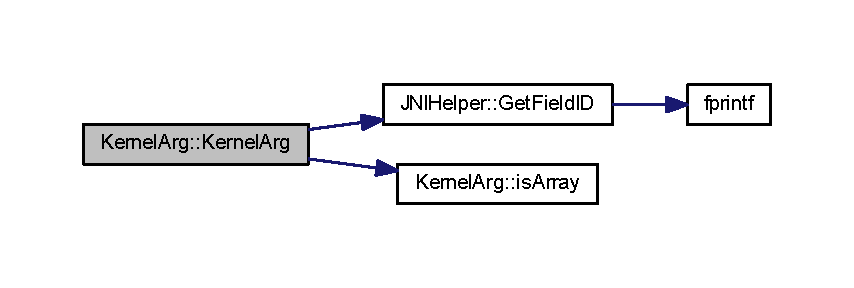
\includegraphics[width=350pt]{class_kernel_arg_ae64310c9ca39693e96f97c78d2e484fa_cgraph}
\end{center}
\end{figure}


\hypertarget{class_kernel_arg_acce352eb369167bfe41b7053fb13cc05}{\index{Kernel\-Arg@{Kernel\-Arg}!$\sim$\-Kernel\-Arg@{$\sim$\-Kernel\-Arg}}
\index{$\sim$\-Kernel\-Arg@{$\sim$\-Kernel\-Arg}!KernelArg@{Kernel\-Arg}}
\subsubsection[{$\sim$\-Kernel\-Arg}]{\setlength{\rightskip}{0pt plus 5cm}Kernel\-Arg\-::$\sim$\-Kernel\-Arg (
\begin{DoxyParamCaption}
{}
\end{DoxyParamCaption}
)\hspace{0.3cm}{\ttfamily [inline]}}}\label{class_kernel_arg_acce352eb369167bfe41b7053fb13cc05}


\subsection{Member Function Documentation}
\hypertarget{class_kernel_arg_ae5df1dec0f6ec684d58b2adf23dd1845}{\index{Kernel\-Arg@{Kernel\-Arg}!clear\-Explicit\-Buffer\-Bit@{clear\-Explicit\-Buffer\-Bit}}
\index{clear\-Explicit\-Buffer\-Bit@{clear\-Explicit\-Buffer\-Bit}!KernelArg@{Kernel\-Arg}}
\subsubsection[{clear\-Explicit\-Buffer\-Bit}]{\setlength{\rightskip}{0pt plus 5cm}void Kernel\-Arg\-::clear\-Explicit\-Buffer\-Bit (
\begin{DoxyParamCaption}
\item[{J\-N\-I\-Env $\ast$}]{jenv}
\end{DoxyParamCaption}
)\hspace{0.3cm}{\ttfamily [inline]}}}\label{class_kernel_arg_ae5df1dec0f6ec684d58b2adf23dd1845}


Here is the caller graph for this function\-:
\nopagebreak
\begin{figure}[H]
\begin{center}
\leavevmode
\includegraphics[width=350pt]{class_kernel_arg_ae5df1dec0f6ec684d58b2adf23dd1845_icgraph}
\end{center}
\end{figure}


\hypertarget{class_kernel_arg_a051e9470c1ffcf16b8116fb29f6e0a94}{\index{Kernel\-Arg@{Kernel\-Arg}!get\-Primitive@{get\-Primitive}}
\index{get\-Primitive@{get\-Primitive}!KernelArg@{Kernel\-Arg}}
\subsubsection[{get\-Primitive}]{\setlength{\rightskip}{0pt plus 5cm}template$<$typename T $>$ void Kernel\-Arg\-::get\-Primitive (
\begin{DoxyParamCaption}
\item[{J\-N\-I\-Env $\ast$}]{jenv, }
\item[{int}]{arg\-Idx, }
\item[{int}]{arg\-Pos, }
\item[{bool}]{verbose, }
\item[{T $\ast$}]{value}
\end{DoxyParamCaption}
)\hspace{0.3cm}{\ttfamily [inline]}, {\ttfamily [private]}}}\label{class_kernel_arg_a051e9470c1ffcf16b8116fb29f6e0a94}


Here is the call graph for this function\-:
\nopagebreak
\begin{figure}[H]
\begin{center}
\leavevmode
\includegraphics[width=350pt]{class_kernel_arg_a051e9470c1ffcf16b8116fb29f6e0a94_cgraph}
\end{center}
\end{figure}




Here is the caller graph for this function\-:
\nopagebreak
\begin{figure}[H]
\begin{center}
\leavevmode
\includegraphics[width=350pt]{class_kernel_arg_a051e9470c1ffcf16b8116fb29f6e0a94_icgraph}
\end{center}
\end{figure}


\hypertarget{class_kernel_arg_a8552d2619bff1029fb9808f97177e7b7}{\index{Kernel\-Arg@{Kernel\-Arg}!get\-Primitive\-Value@{get\-Primitive\-Value}}
\index{get\-Primitive\-Value@{get\-Primitive\-Value}!KernelArg@{Kernel\-Arg}}
\subsubsection[{get\-Primitive\-Value}]{\setlength{\rightskip}{0pt plus 5cm}void Kernel\-Arg\-::get\-Primitive\-Value (
\begin{DoxyParamCaption}
\item[{J\-N\-I\-Env $\ast$}]{jenv, }
\item[{jfloat $\ast$}]{value}
\end{DoxyParamCaption}
)\hspace{0.3cm}{\ttfamily [private]}}}\label{class_kernel_arg_a8552d2619bff1029fb9808f97177e7b7}


Here is the caller graph for this function\-:
\nopagebreak
\begin{figure}[H]
\begin{center}
\leavevmode
\includegraphics[width=350pt]{class_kernel_arg_a8552d2619bff1029fb9808f97177e7b7_icgraph}
\end{center}
\end{figure}


\hypertarget{class_kernel_arg_a38b8d4a21460c090e0ade4cf833a4563}{\index{Kernel\-Arg@{Kernel\-Arg}!get\-Primitive\-Value@{get\-Primitive\-Value}}
\index{get\-Primitive\-Value@{get\-Primitive\-Value}!KernelArg@{Kernel\-Arg}}
\subsubsection[{get\-Primitive\-Value}]{\setlength{\rightskip}{0pt plus 5cm}void Kernel\-Arg\-::get\-Primitive\-Value (
\begin{DoxyParamCaption}
\item[{J\-N\-I\-Env $\ast$}]{jenv, }
\item[{jint $\ast$}]{value}
\end{DoxyParamCaption}
)\hspace{0.3cm}{\ttfamily [private]}}}\label{class_kernel_arg_a38b8d4a21460c090e0ade4cf833a4563}
\hypertarget{class_kernel_arg_a7fb6ada5ddd53e616a8c3a131103f9e9}{\index{Kernel\-Arg@{Kernel\-Arg}!get\-Primitive\-Value@{get\-Primitive\-Value}}
\index{get\-Primitive\-Value@{get\-Primitive\-Value}!KernelArg@{Kernel\-Arg}}
\subsubsection[{get\-Primitive\-Value}]{\setlength{\rightskip}{0pt plus 5cm}void Kernel\-Arg\-::get\-Primitive\-Value (
\begin{DoxyParamCaption}
\item[{J\-N\-I\-Env $\ast$}]{jenv, }
\item[{jboolean $\ast$}]{value}
\end{DoxyParamCaption}
)\hspace{0.3cm}{\ttfamily [private]}}}\label{class_kernel_arg_a7fb6ada5ddd53e616a8c3a131103f9e9}
\hypertarget{class_kernel_arg_aa465cfbea45ce00205768609ed3e9d06}{\index{Kernel\-Arg@{Kernel\-Arg}!get\-Primitive\-Value@{get\-Primitive\-Value}}
\index{get\-Primitive\-Value@{get\-Primitive\-Value}!KernelArg@{Kernel\-Arg}}
\subsubsection[{get\-Primitive\-Value}]{\setlength{\rightskip}{0pt plus 5cm}void Kernel\-Arg\-::get\-Primitive\-Value (
\begin{DoxyParamCaption}
\item[{J\-N\-I\-Env $\ast$}]{jenv, }
\item[{jbyte $\ast$}]{value}
\end{DoxyParamCaption}
)\hspace{0.3cm}{\ttfamily [private]}}}\label{class_kernel_arg_aa465cfbea45ce00205768609ed3e9d06}
\hypertarget{class_kernel_arg_a9c165792868716005957ee3c1bca7977}{\index{Kernel\-Arg@{Kernel\-Arg}!get\-Primitive\-Value@{get\-Primitive\-Value}}
\index{get\-Primitive\-Value@{get\-Primitive\-Value}!KernelArg@{Kernel\-Arg}}
\subsubsection[{get\-Primitive\-Value}]{\setlength{\rightskip}{0pt plus 5cm}void Kernel\-Arg\-::get\-Primitive\-Value (
\begin{DoxyParamCaption}
\item[{J\-N\-I\-Env $\ast$}]{jenv, }
\item[{jlong $\ast$}]{value}
\end{DoxyParamCaption}
)\hspace{0.3cm}{\ttfamily [private]}}}\label{class_kernel_arg_a9c165792868716005957ee3c1bca7977}
\hypertarget{class_kernel_arg_a2e4c14bd27f43be4c1482c4714e6c926}{\index{Kernel\-Arg@{Kernel\-Arg}!get\-Primitive\-Value@{get\-Primitive\-Value}}
\index{get\-Primitive\-Value@{get\-Primitive\-Value}!KernelArg@{Kernel\-Arg}}
\subsubsection[{get\-Primitive\-Value}]{\setlength{\rightskip}{0pt plus 5cm}void Kernel\-Arg\-::get\-Primitive\-Value (
\begin{DoxyParamCaption}
\item[{J\-N\-I\-Env $\ast$}]{jenv, }
\item[{jdouble $\ast$}]{value}
\end{DoxyParamCaption}
)\hspace{0.3cm}{\ttfamily [private]}}}\label{class_kernel_arg_a2e4c14bd27f43be4c1482c4714e6c926}
\hypertarget{class_kernel_arg_ac545f1203b8ba8ab301b8e3ce60357eb}{\index{Kernel\-Arg@{Kernel\-Arg}!get\-Static\-Primitive\-Value@{get\-Static\-Primitive\-Value}}
\index{get\-Static\-Primitive\-Value@{get\-Static\-Primitive\-Value}!KernelArg@{Kernel\-Arg}}
\subsubsection[{get\-Static\-Primitive\-Value}]{\setlength{\rightskip}{0pt plus 5cm}void Kernel\-Arg\-::get\-Static\-Primitive\-Value (
\begin{DoxyParamCaption}
\item[{J\-N\-I\-Env $\ast$}]{jenv, }
\item[{jfloat $\ast$}]{value}
\end{DoxyParamCaption}
)\hspace{0.3cm}{\ttfamily [private]}}}\label{class_kernel_arg_ac545f1203b8ba8ab301b8e3ce60357eb}


Here is the caller graph for this function\-:
\nopagebreak
\begin{figure}[H]
\begin{center}
\leavevmode
\includegraphics[width=350pt]{class_kernel_arg_ac545f1203b8ba8ab301b8e3ce60357eb_icgraph}
\end{center}
\end{figure}


\hypertarget{class_kernel_arg_a38128b0843f283bd4af95ba2f301e9d1}{\index{Kernel\-Arg@{Kernel\-Arg}!get\-Static\-Primitive\-Value@{get\-Static\-Primitive\-Value}}
\index{get\-Static\-Primitive\-Value@{get\-Static\-Primitive\-Value}!KernelArg@{Kernel\-Arg}}
\subsubsection[{get\-Static\-Primitive\-Value}]{\setlength{\rightskip}{0pt plus 5cm}void Kernel\-Arg\-::get\-Static\-Primitive\-Value (
\begin{DoxyParamCaption}
\item[{J\-N\-I\-Env $\ast$}]{jenv, }
\item[{jint $\ast$}]{value}
\end{DoxyParamCaption}
)\hspace{0.3cm}{\ttfamily [private]}}}\label{class_kernel_arg_a38128b0843f283bd4af95ba2f301e9d1}
\hypertarget{class_kernel_arg_a726eab9b0864237a01cea9263268cec5}{\index{Kernel\-Arg@{Kernel\-Arg}!get\-Static\-Primitive\-Value@{get\-Static\-Primitive\-Value}}
\index{get\-Static\-Primitive\-Value@{get\-Static\-Primitive\-Value}!KernelArg@{Kernel\-Arg}}
\subsubsection[{get\-Static\-Primitive\-Value}]{\setlength{\rightskip}{0pt plus 5cm}void Kernel\-Arg\-::get\-Static\-Primitive\-Value (
\begin{DoxyParamCaption}
\item[{J\-N\-I\-Env $\ast$}]{jenv, }
\item[{jboolean $\ast$}]{value}
\end{DoxyParamCaption}
)\hspace{0.3cm}{\ttfamily [private]}}}\label{class_kernel_arg_a726eab9b0864237a01cea9263268cec5}
\hypertarget{class_kernel_arg_a86d9b170e6049ea5419946abfb8630aa}{\index{Kernel\-Arg@{Kernel\-Arg}!get\-Static\-Primitive\-Value@{get\-Static\-Primitive\-Value}}
\index{get\-Static\-Primitive\-Value@{get\-Static\-Primitive\-Value}!KernelArg@{Kernel\-Arg}}
\subsubsection[{get\-Static\-Primitive\-Value}]{\setlength{\rightskip}{0pt plus 5cm}void Kernel\-Arg\-::get\-Static\-Primitive\-Value (
\begin{DoxyParamCaption}
\item[{J\-N\-I\-Env $\ast$}]{jenv, }
\item[{jbyte $\ast$}]{value}
\end{DoxyParamCaption}
)\hspace{0.3cm}{\ttfamily [private]}}}\label{class_kernel_arg_a86d9b170e6049ea5419946abfb8630aa}
\hypertarget{class_kernel_arg_ac88ed8ecdb1b1386a1babce46a8fd82b}{\index{Kernel\-Arg@{Kernel\-Arg}!get\-Static\-Primitive\-Value@{get\-Static\-Primitive\-Value}}
\index{get\-Static\-Primitive\-Value@{get\-Static\-Primitive\-Value}!KernelArg@{Kernel\-Arg}}
\subsubsection[{get\-Static\-Primitive\-Value}]{\setlength{\rightskip}{0pt plus 5cm}void Kernel\-Arg\-::get\-Static\-Primitive\-Value (
\begin{DoxyParamCaption}
\item[{J\-N\-I\-Env $\ast$}]{jenv, }
\item[{jlong $\ast$}]{value}
\end{DoxyParamCaption}
)\hspace{0.3cm}{\ttfamily [private]}}}\label{class_kernel_arg_ac88ed8ecdb1b1386a1babce46a8fd82b}
\hypertarget{class_kernel_arg_a33f565e75e4ab63bf9e575e34b8495d3}{\index{Kernel\-Arg@{Kernel\-Arg}!get\-Static\-Primitive\-Value@{get\-Static\-Primitive\-Value}}
\index{get\-Static\-Primitive\-Value@{get\-Static\-Primitive\-Value}!KernelArg@{Kernel\-Arg}}
\subsubsection[{get\-Static\-Primitive\-Value}]{\setlength{\rightskip}{0pt plus 5cm}void Kernel\-Arg\-::get\-Static\-Primitive\-Value (
\begin{DoxyParamCaption}
\item[{J\-N\-I\-Env $\ast$}]{jenv, }
\item[{jdouble $\ast$}]{value}
\end{DoxyParamCaption}
)\hspace{0.3cm}{\ttfamily [private]}}}\label{class_kernel_arg_a33f565e75e4ab63bf9e575e34b8495d3}
\hypertarget{class_kernel_arg_a88b9eef8162da192c5d0245519538417}{\index{Kernel\-Arg@{Kernel\-Arg}!get\-Type\-Name@{get\-Type\-Name}}
\index{get\-Type\-Name@{get\-Type\-Name}!KernelArg@{Kernel\-Arg}}
\subsubsection[{get\-Type\-Name}]{\setlength{\rightskip}{0pt plus 5cm}const char $\ast$ Kernel\-Arg\-::get\-Type\-Name (
\begin{DoxyParamCaption}
{}
\end{DoxyParamCaption}
)\hspace{0.3cm}{\ttfamily [private]}}}\label{class_kernel_arg_a88b9eef8162da192c5d0245519538417}


Here is the call graph for this function\-:
\nopagebreak
\begin{figure}[H]
\begin{center}
\leavevmode
\includegraphics[width=350pt]{class_kernel_arg_a88b9eef8162da192c5d0245519538417_cgraph}
\end{center}
\end{figure}




Here is the caller graph for this function\-:
\nopagebreak
\begin{figure}[H]
\begin{center}
\leavevmode
\includegraphics[width=350pt]{class_kernel_arg_a88b9eef8162da192c5d0245519538417_icgraph}
\end{center}
\end{figure}


\hypertarget{class_kernel_arg_a49be011b2c8ee9f85d507521854fb4f8}{\index{Kernel\-Arg@{Kernel\-Arg}!is\-Aparapi\-Buf@{is\-Aparapi\-Buf}}
\index{is\-Aparapi\-Buf@{is\-Aparapi\-Buf}!KernelArg@{Kernel\-Arg}}
\subsubsection[{is\-Aparapi\-Buf}]{\setlength{\rightskip}{0pt plus 5cm}int Kernel\-Arg\-::is\-Aparapi\-Buf (
\begin{DoxyParamCaption}
{}
\end{DoxyParamCaption}
)\hspace{0.3cm}{\ttfamily [inline]}}}\label{class_kernel_arg_a49be011b2c8ee9f85d507521854fb4f8}


Here is the caller graph for this function\-:
\nopagebreak
\begin{figure}[H]
\begin{center}
\leavevmode
\includegraphics[width=350pt]{class_kernel_arg_a49be011b2c8ee9f85d507521854fb4f8_icgraph}
\end{center}
\end{figure}


\hypertarget{class_kernel_arg_a5d1c17442e6f96aa1aeb834a82ed6950}{\index{Kernel\-Arg@{Kernel\-Arg}!is\-Array@{is\-Array}}
\index{is\-Array@{is\-Array}!KernelArg@{Kernel\-Arg}}
\subsubsection[{is\-Array}]{\setlength{\rightskip}{0pt plus 5cm}int Kernel\-Arg\-::is\-Array (
\begin{DoxyParamCaption}
{}
\end{DoxyParamCaption}
)\hspace{0.3cm}{\ttfamily [inline]}}}\label{class_kernel_arg_a5d1c17442e6f96aa1aeb834a82ed6950}


Here is the caller graph for this function\-:
\nopagebreak
\begin{figure}[H]
\begin{center}
\leavevmode
\includegraphics[width=350pt]{class_kernel_arg_a5d1c17442e6f96aa1aeb834a82ed6950_icgraph}
\end{center}
\end{figure}


\hypertarget{class_kernel_arg_a8e5e4bf1b90efaf6a805028f831968da}{\index{Kernel\-Arg@{Kernel\-Arg}!is\-Backed\-By\-Array@{is\-Backed\-By\-Array}}
\index{is\-Backed\-By\-Array@{is\-Backed\-By\-Array}!KernelArg@{Kernel\-Arg}}
\subsubsection[{is\-Backed\-By\-Array}]{\setlength{\rightskip}{0pt plus 5cm}int Kernel\-Arg\-::is\-Backed\-By\-Array (
\begin{DoxyParamCaption}
{}
\end{DoxyParamCaption}
)\hspace{0.3cm}{\ttfamily [inline]}}}\label{class_kernel_arg_a8e5e4bf1b90efaf6a805028f831968da}


Here is the call graph for this function\-:
\nopagebreak
\begin{figure}[H]
\begin{center}
\leavevmode
\includegraphics[width=350pt]{class_kernel_arg_a8e5e4bf1b90efaf6a805028f831968da_cgraph}
\end{center}
\end{figure}




Here is the caller graph for this function\-:
\nopagebreak
\begin{figure}[H]
\begin{center}
\leavevmode
\includegraphics[width=350pt]{class_kernel_arg_a8e5e4bf1b90efaf6a805028f831968da_icgraph}
\end{center}
\end{figure}


\hypertarget{class_kernel_arg_a6eea48cf98d46f8d50ee53a1edcc195f}{\index{Kernel\-Arg@{Kernel\-Arg}!is\-Boolean@{is\-Boolean}}
\index{is\-Boolean@{is\-Boolean}!KernelArg@{Kernel\-Arg}}
\subsubsection[{is\-Boolean}]{\setlength{\rightskip}{0pt plus 5cm}int Kernel\-Arg\-::is\-Boolean (
\begin{DoxyParamCaption}
{}
\end{DoxyParamCaption}
)\hspace{0.3cm}{\ttfamily [inline]}}}\label{class_kernel_arg_a6eea48cf98d46f8d50ee53a1edcc195f}


Here is the caller graph for this function\-:
\nopagebreak
\begin{figure}[H]
\begin{center}
\leavevmode
\includegraphics[width=350pt]{class_kernel_arg_a6eea48cf98d46f8d50ee53a1edcc195f_icgraph}
\end{center}
\end{figure}


\hypertarget{class_kernel_arg_ac4905b9b405fc2a93d05127516d6777f}{\index{Kernel\-Arg@{Kernel\-Arg}!is\-Byte@{is\-Byte}}
\index{is\-Byte@{is\-Byte}!KernelArg@{Kernel\-Arg}}
\subsubsection[{is\-Byte}]{\setlength{\rightskip}{0pt plus 5cm}int Kernel\-Arg\-::is\-Byte (
\begin{DoxyParamCaption}
{}
\end{DoxyParamCaption}
)\hspace{0.3cm}{\ttfamily [inline]}}}\label{class_kernel_arg_ac4905b9b405fc2a93d05127516d6777f}


Here is the caller graph for this function\-:
\nopagebreak
\begin{figure}[H]
\begin{center}
\leavevmode
\includegraphics[width=350pt]{class_kernel_arg_ac4905b9b405fc2a93d05127516d6777f_icgraph}
\end{center}
\end{figure}


\hypertarget{class_kernel_arg_a266bef2508f3aa4c1f2e670b7658f05e}{\index{Kernel\-Arg@{Kernel\-Arg}!is\-Constant@{is\-Constant}}
\index{is\-Constant@{is\-Constant}!KernelArg@{Kernel\-Arg}}
\subsubsection[{is\-Constant}]{\setlength{\rightskip}{0pt plus 5cm}int Kernel\-Arg\-::is\-Constant (
\begin{DoxyParamCaption}
{}
\end{DoxyParamCaption}
)\hspace{0.3cm}{\ttfamily [inline]}}}\label{class_kernel_arg_a266bef2508f3aa4c1f2e670b7658f05e}


Here is the caller graph for this function\-:
\nopagebreak
\begin{figure}[H]
\begin{center}
\leavevmode
\includegraphics[width=350pt]{class_kernel_arg_a266bef2508f3aa4c1f2e670b7658f05e_icgraph}
\end{center}
\end{figure}


\hypertarget{class_kernel_arg_ac8b08f0b2210d4217dac92f27389f330}{\index{Kernel\-Arg@{Kernel\-Arg}!is\-Double@{is\-Double}}
\index{is\-Double@{is\-Double}!KernelArg@{Kernel\-Arg}}
\subsubsection[{is\-Double}]{\setlength{\rightskip}{0pt plus 5cm}int Kernel\-Arg\-::is\-Double (
\begin{DoxyParamCaption}
{}
\end{DoxyParamCaption}
)\hspace{0.3cm}{\ttfamily [inline]}}}\label{class_kernel_arg_ac8b08f0b2210d4217dac92f27389f330}


Here is the caller graph for this function\-:
\nopagebreak
\begin{figure}[H]
\begin{center}
\leavevmode
\includegraphics[width=350pt]{class_kernel_arg_ac8b08f0b2210d4217dac92f27389f330_icgraph}
\end{center}
\end{figure}


\hypertarget{class_kernel_arg_a14a83444c553bc8b8458223af8339e3d}{\index{Kernel\-Arg@{Kernel\-Arg}!is\-Explicit@{is\-Explicit}}
\index{is\-Explicit@{is\-Explicit}!KernelArg@{Kernel\-Arg}}
\subsubsection[{is\-Explicit}]{\setlength{\rightskip}{0pt plus 5cm}int Kernel\-Arg\-::is\-Explicit (
\begin{DoxyParamCaption}
{}
\end{DoxyParamCaption}
)\hspace{0.3cm}{\ttfamily [inline]}}}\label{class_kernel_arg_a14a83444c553bc8b8458223af8339e3d}


Here is the caller graph for this function\-:
\nopagebreak
\begin{figure}[H]
\begin{center}
\leavevmode
\includegraphics[width=350pt]{class_kernel_arg_a14a83444c553bc8b8458223af8339e3d_icgraph}
\end{center}
\end{figure}


\hypertarget{class_kernel_arg_a080a2a1cae98156eec8dff6409b3c5f2}{\index{Kernel\-Arg@{Kernel\-Arg}!is\-Explicit\-Write@{is\-Explicit\-Write}}
\index{is\-Explicit\-Write@{is\-Explicit\-Write}!KernelArg@{Kernel\-Arg}}
\subsubsection[{is\-Explicit\-Write}]{\setlength{\rightskip}{0pt plus 5cm}int Kernel\-Arg\-::is\-Explicit\-Write (
\begin{DoxyParamCaption}
{}
\end{DoxyParamCaption}
)\hspace{0.3cm}{\ttfamily [inline]}}}\label{class_kernel_arg_a080a2a1cae98156eec8dff6409b3c5f2}


Here is the caller graph for this function\-:
\nopagebreak
\begin{figure}[H]
\begin{center}
\leavevmode
\includegraphics[width=350pt]{class_kernel_arg_a080a2a1cae98156eec8dff6409b3c5f2_icgraph}
\end{center}
\end{figure}


\hypertarget{class_kernel_arg_a80c129f34138199a1d6495e509a769f1}{\index{Kernel\-Arg@{Kernel\-Arg}!is\-Float@{is\-Float}}
\index{is\-Float@{is\-Float}!KernelArg@{Kernel\-Arg}}
\subsubsection[{is\-Float}]{\setlength{\rightskip}{0pt plus 5cm}int Kernel\-Arg\-::is\-Float (
\begin{DoxyParamCaption}
{}
\end{DoxyParamCaption}
)\hspace{0.3cm}{\ttfamily [inline]}}}\label{class_kernel_arg_a80c129f34138199a1d6495e509a769f1}


Here is the caller graph for this function\-:
\nopagebreak
\begin{figure}[H]
\begin{center}
\leavevmode
\includegraphics[width=350pt]{class_kernel_arg_a80c129f34138199a1d6495e509a769f1_icgraph}
\end{center}
\end{figure}


\hypertarget{class_kernel_arg_ae38da6f0073ce862e16c2f21ef451d0b}{\index{Kernel\-Arg@{Kernel\-Arg}!is\-Global@{is\-Global}}
\index{is\-Global@{is\-Global}!KernelArg@{Kernel\-Arg}}
\subsubsection[{is\-Global}]{\setlength{\rightskip}{0pt plus 5cm}int Kernel\-Arg\-::is\-Global (
\begin{DoxyParamCaption}
{}
\end{DoxyParamCaption}
)\hspace{0.3cm}{\ttfamily [inline]}}}\label{class_kernel_arg_ae38da6f0073ce862e16c2f21ef451d0b}


Here is the caller graph for this function\-:
\nopagebreak
\begin{figure}[H]
\begin{center}
\leavevmode
\includegraphics[width=350pt]{class_kernel_arg_ae38da6f0073ce862e16c2f21ef451d0b_icgraph}
\end{center}
\end{figure}


\hypertarget{class_kernel_arg_ab8a775d67ecb9bf9c8ad4654fe7c3f58}{\index{Kernel\-Arg@{Kernel\-Arg}!is\-Implicit@{is\-Implicit}}
\index{is\-Implicit@{is\-Implicit}!KernelArg@{Kernel\-Arg}}
\subsubsection[{is\-Implicit}]{\setlength{\rightskip}{0pt plus 5cm}int Kernel\-Arg\-::is\-Implicit (
\begin{DoxyParamCaption}
{}
\end{DoxyParamCaption}
)\hspace{0.3cm}{\ttfamily [inline]}}}\label{class_kernel_arg_ab8a775d67ecb9bf9c8ad4654fe7c3f58}


Here is the call graph for this function\-:
\nopagebreak
\begin{figure}[H]
\begin{center}
\leavevmode
\includegraphics[width=326pt]{class_kernel_arg_ab8a775d67ecb9bf9c8ad4654fe7c3f58_cgraph}
\end{center}
\end{figure}




Here is the caller graph for this function\-:
\nopagebreak
\begin{figure}[H]
\begin{center}
\leavevmode
\includegraphics[width=350pt]{class_kernel_arg_ab8a775d67ecb9bf9c8ad4654fe7c3f58_icgraph}
\end{center}
\end{figure}


\hypertarget{class_kernel_arg_adcf1efdd8a1c804db121c7f466472716}{\index{Kernel\-Arg@{Kernel\-Arg}!is\-Int@{is\-Int}}
\index{is\-Int@{is\-Int}!KernelArg@{Kernel\-Arg}}
\subsubsection[{is\-Int}]{\setlength{\rightskip}{0pt plus 5cm}int Kernel\-Arg\-::is\-Int (
\begin{DoxyParamCaption}
{}
\end{DoxyParamCaption}
)\hspace{0.3cm}{\ttfamily [inline]}}}\label{class_kernel_arg_adcf1efdd8a1c804db121c7f466472716}


Here is the caller graph for this function\-:
\nopagebreak
\begin{figure}[H]
\begin{center}
\leavevmode
\includegraphics[width=350pt]{class_kernel_arg_adcf1efdd8a1c804db121c7f466472716_icgraph}
\end{center}
\end{figure}


\hypertarget{class_kernel_arg_ab4e2866a831ea45934cec64566fb4816}{\index{Kernel\-Arg@{Kernel\-Arg}!is\-Local@{is\-Local}}
\index{is\-Local@{is\-Local}!KernelArg@{Kernel\-Arg}}
\subsubsection[{is\-Local}]{\setlength{\rightskip}{0pt plus 5cm}int Kernel\-Arg\-::is\-Local (
\begin{DoxyParamCaption}
{}
\end{DoxyParamCaption}
)\hspace{0.3cm}{\ttfamily [inline]}}}\label{class_kernel_arg_ab4e2866a831ea45934cec64566fb4816}


Here is the caller graph for this function\-:
\nopagebreak
\begin{figure}[H]
\begin{center}
\leavevmode
\includegraphics[width=284pt]{class_kernel_arg_ab4e2866a831ea45934cec64566fb4816_icgraph}
\end{center}
\end{figure}


\hypertarget{class_kernel_arg_a92b487c069a5e65ba49d56ab867329a3}{\index{Kernel\-Arg@{Kernel\-Arg}!is\-Long@{is\-Long}}
\index{is\-Long@{is\-Long}!KernelArg@{Kernel\-Arg}}
\subsubsection[{is\-Long}]{\setlength{\rightskip}{0pt plus 5cm}int Kernel\-Arg\-::is\-Long (
\begin{DoxyParamCaption}
{}
\end{DoxyParamCaption}
)\hspace{0.3cm}{\ttfamily [inline]}}}\label{class_kernel_arg_a92b487c069a5e65ba49d56ab867329a3}


Here is the caller graph for this function\-:
\nopagebreak
\begin{figure}[H]
\begin{center}
\leavevmode
\includegraphics[width=350pt]{class_kernel_arg_a92b487c069a5e65ba49d56ab867329a3_icgraph}
\end{center}
\end{figure}


\hypertarget{class_kernel_arg_aa1002b4a71aaa86b3089beee7f84d325}{\index{Kernel\-Arg@{Kernel\-Arg}!is\-Mutable\-By\-Kernel@{is\-Mutable\-By\-Kernel}}
\index{is\-Mutable\-By\-Kernel@{is\-Mutable\-By\-Kernel}!KernelArg@{Kernel\-Arg}}
\subsubsection[{is\-Mutable\-By\-Kernel}]{\setlength{\rightskip}{0pt plus 5cm}int Kernel\-Arg\-::is\-Mutable\-By\-Kernel (
\begin{DoxyParamCaption}
{}
\end{DoxyParamCaption}
)\hspace{0.3cm}{\ttfamily [inline]}}}\label{class_kernel_arg_aa1002b4a71aaa86b3089beee7f84d325}


Here is the caller graph for this function\-:
\nopagebreak
\begin{figure}[H]
\begin{center}
\leavevmode
\includegraphics[width=350pt]{class_kernel_arg_aa1002b4a71aaa86b3089beee7f84d325_icgraph}
\end{center}
\end{figure}


\hypertarget{class_kernel_arg_a11ed28ef2892d605343092d77570c859}{\index{Kernel\-Arg@{Kernel\-Arg}!is\-Primitive@{is\-Primitive}}
\index{is\-Primitive@{is\-Primitive}!KernelArg@{Kernel\-Arg}}
\subsubsection[{is\-Primitive}]{\setlength{\rightskip}{0pt plus 5cm}int Kernel\-Arg\-::is\-Primitive (
\begin{DoxyParamCaption}
{}
\end{DoxyParamCaption}
)\hspace{0.3cm}{\ttfamily [inline]}}}\label{class_kernel_arg_a11ed28ef2892d605343092d77570c859}


Here is the caller graph for this function\-:
\nopagebreak
\begin{figure}[H]
\begin{center}
\leavevmode
\includegraphics[width=350pt]{class_kernel_arg_a11ed28ef2892d605343092d77570c859_icgraph}
\end{center}
\end{figure}


\hypertarget{class_kernel_arg_a164df3cf2ae35d7b53f5796e46c01fe5}{\index{Kernel\-Arg@{Kernel\-Arg}!is\-Read\-By\-Kernel@{is\-Read\-By\-Kernel}}
\index{is\-Read\-By\-Kernel@{is\-Read\-By\-Kernel}!KernelArg@{Kernel\-Arg}}
\subsubsection[{is\-Read\-By\-Kernel}]{\setlength{\rightskip}{0pt plus 5cm}int Kernel\-Arg\-::is\-Read\-By\-Kernel (
\begin{DoxyParamCaption}
{}
\end{DoxyParamCaption}
)\hspace{0.3cm}{\ttfamily [inline]}}}\label{class_kernel_arg_a164df3cf2ae35d7b53f5796e46c01fe5}


Here is the caller graph for this function\-:
\nopagebreak
\begin{figure}[H]
\begin{center}
\leavevmode
\includegraphics[width=350pt]{class_kernel_arg_a164df3cf2ae35d7b53f5796e46c01fe5_icgraph}
\end{center}
\end{figure}


\hypertarget{class_kernel_arg_a0b9156ed4ddabff7c63b39973c4f81a2}{\index{Kernel\-Arg@{Kernel\-Arg}!is\-Short@{is\-Short}}
\index{is\-Short@{is\-Short}!KernelArg@{Kernel\-Arg}}
\subsubsection[{is\-Short}]{\setlength{\rightskip}{0pt plus 5cm}int Kernel\-Arg\-::is\-Short (
\begin{DoxyParamCaption}
{}
\end{DoxyParamCaption}
)\hspace{0.3cm}{\ttfamily [inline]}}}\label{class_kernel_arg_a0b9156ed4ddabff7c63b39973c4f81a2}
\hypertarget{class_kernel_arg_aae70fdc4496f4c2f3847dc01e3acf97d}{\index{Kernel\-Arg@{Kernel\-Arg}!is\-Static@{is\-Static}}
\index{is\-Static@{is\-Static}!KernelArg@{Kernel\-Arg}}
\subsubsection[{is\-Static}]{\setlength{\rightskip}{0pt plus 5cm}int Kernel\-Arg\-::is\-Static (
\begin{DoxyParamCaption}
{}
\end{DoxyParamCaption}
)\hspace{0.3cm}{\ttfamily [inline]}}}\label{class_kernel_arg_aae70fdc4496f4c2f3847dc01e3acf97d}


Here is the caller graph for this function\-:
\nopagebreak
\begin{figure}[H]
\begin{center}
\leavevmode
\includegraphics[width=350pt]{class_kernel_arg_aae70fdc4496f4c2f3847dc01e3acf97d_icgraph}
\end{center}
\end{figure}


\hypertarget{class_kernel_arg_a789786a4bb65c3ac76299474ee371c87}{\index{Kernel\-Arg@{Kernel\-Arg}!need\-To\-Enqueue\-Read@{need\-To\-Enqueue\-Read}}
\index{need\-To\-Enqueue\-Read@{need\-To\-Enqueue\-Read}!KernelArg@{Kernel\-Arg}}
\subsubsection[{need\-To\-Enqueue\-Read}]{\setlength{\rightskip}{0pt plus 5cm}int Kernel\-Arg\-::need\-To\-Enqueue\-Read (
\begin{DoxyParamCaption}
{}
\end{DoxyParamCaption}
)\hspace{0.3cm}{\ttfamily [inline]}}}\label{class_kernel_arg_a789786a4bb65c3ac76299474ee371c87}


Here is the call graph for this function\-:
\nopagebreak
\begin{figure}[H]
\begin{center}
\leavevmode
\includegraphics[width=350pt]{class_kernel_arg_a789786a4bb65c3ac76299474ee371c87_cgraph}
\end{center}
\end{figure}




Here is the caller graph for this function\-:
\nopagebreak
\begin{figure}[H]
\begin{center}
\leavevmode
\includegraphics[width=350pt]{class_kernel_arg_a789786a4bb65c3ac76299474ee371c87_icgraph}
\end{center}
\end{figure}


\hypertarget{class_kernel_arg_a42f6eead7b43c2e0839aae776c09bcb3}{\index{Kernel\-Arg@{Kernel\-Arg}!need\-To\-Enqueue\-Write@{need\-To\-Enqueue\-Write}}
\index{need\-To\-Enqueue\-Write@{need\-To\-Enqueue\-Write}!KernelArg@{Kernel\-Arg}}
\subsubsection[{need\-To\-Enqueue\-Write}]{\setlength{\rightskip}{0pt plus 5cm}int Kernel\-Arg\-::need\-To\-Enqueue\-Write (
\begin{DoxyParamCaption}
{}
\end{DoxyParamCaption}
)\hspace{0.3cm}{\ttfamily [inline]}}}\label{class_kernel_arg_a42f6eead7b43c2e0839aae776c09bcb3}


Here is the call graph for this function\-:
\nopagebreak
\begin{figure}[H]
\begin{center}
\leavevmode
\includegraphics[width=350pt]{class_kernel_arg_a42f6eead7b43c2e0839aae776c09bcb3_cgraph}
\end{center}
\end{figure}




Here is the caller graph for this function\-:
\nopagebreak
\begin{figure}[H]
\begin{center}
\leavevmode
\includegraphics[width=324pt]{class_kernel_arg_a42f6eead7b43c2e0839aae776c09bcb3_icgraph}
\end{center}
\end{figure}


\hypertarget{class_kernel_arg_a6fc2b16f01ddb5fba224d38fabc128cf}{\index{Kernel\-Arg@{Kernel\-Arg}!pin@{pin}}
\index{pin@{pin}!KernelArg@{Kernel\-Arg}}
\subsubsection[{pin}]{\setlength{\rightskip}{0pt plus 5cm}void Kernel\-Arg\-::pin (
\begin{DoxyParamCaption}
\item[{J\-N\-I\-Env $\ast$}]{jenv}
\end{DoxyParamCaption}
)\hspace{0.3cm}{\ttfamily [inline]}}}\label{class_kernel_arg_a6fc2b16f01ddb5fba224d38fabc128cf}


Here is the call graph for this function\-:
\nopagebreak
\begin{figure}[H]
\begin{center}
\leavevmode
\includegraphics[width=278pt]{class_kernel_arg_a6fc2b16f01ddb5fba224d38fabc128cf_cgraph}
\end{center}
\end{figure}




Here is the caller graph for this function\-:
\nopagebreak
\begin{figure}[H]
\begin{center}
\leavevmode
\includegraphics[width=350pt]{class_kernel_arg_a6fc2b16f01ddb5fba224d38fabc128cf_icgraph}
\end{center}
\end{figure}


\hypertarget{class_kernel_arg_a773fa9e962e4c5e72d2cc90f94b5a9c2}{\index{Kernel\-Arg@{Kernel\-Arg}!set\-Local\-Buffer\-Arg@{set\-Local\-Buffer\-Arg}}
\index{set\-Local\-Buffer\-Arg@{set\-Local\-Buffer\-Arg}!KernelArg@{Kernel\-Arg}}
\subsubsection[{set\-Local\-Buffer\-Arg}]{\setlength{\rightskip}{0pt plus 5cm}cl\-\_\-int Kernel\-Arg\-::set\-Local\-Buffer\-Arg (
\begin{DoxyParamCaption}
\item[{J\-N\-I\-Env $\ast$}]{jenv, }
\item[{int}]{arg\-Idx, }
\item[{int}]{arg\-Pos, }
\item[{bool}]{verbose}
\end{DoxyParamCaption}
)}}\label{class_kernel_arg_a773fa9e962e4c5e72d2cc90f94b5a9c2}


Here is the call graph for this function\-:
\nopagebreak
\begin{figure}[H]
\begin{center}
\leavevmode
\includegraphics[width=298pt]{class_kernel_arg_a773fa9e962e4c5e72d2cc90f94b5a9c2_cgraph}
\end{center}
\end{figure}




Here is the caller graph for this function\-:
\nopagebreak
\begin{figure}[H]
\begin{center}
\leavevmode
\includegraphics[width=350pt]{class_kernel_arg_a773fa9e962e4c5e72d2cc90f94b5a9c2_icgraph}
\end{center}
\end{figure}


\hypertarget{class_kernel_arg_aaeb024c19d0269f3a18076bb280c512c}{\index{Kernel\-Arg@{Kernel\-Arg}!set\-Primitive\-Arg@{set\-Primitive\-Arg}}
\index{set\-Primitive\-Arg@{set\-Primitive\-Arg}!KernelArg@{Kernel\-Arg}}
\subsubsection[{set\-Primitive\-Arg}]{\setlength{\rightskip}{0pt plus 5cm}cl\-\_\-int Kernel\-Arg\-::set\-Primitive\-Arg (
\begin{DoxyParamCaption}
\item[{J\-N\-I\-Env $\ast$}]{jenv, }
\item[{int}]{arg\-Idx, }
\item[{int}]{arg\-Pos, }
\item[{bool}]{verbose}
\end{DoxyParamCaption}
)}}\label{class_kernel_arg_aaeb024c19d0269f3a18076bb280c512c}


Here is the call graph for this function\-:
\nopagebreak
\begin{figure}[H]
\begin{center}
\leavevmode
\includegraphics[width=350pt]{class_kernel_arg_aaeb024c19d0269f3a18076bb280c512c_cgraph}
\end{center}
\end{figure}




Here is the caller graph for this function\-:
\nopagebreak
\begin{figure}[H]
\begin{center}
\leavevmode
\includegraphics[width=320pt]{class_kernel_arg_aaeb024c19d0269f3a18076bb280c512c_icgraph}
\end{center}
\end{figure}


\hypertarget{class_kernel_arg_a121239122f29829dd24a8971a207951b}{\index{Kernel\-Arg@{Kernel\-Arg}!sync\-Java\-Array\-Length@{sync\-Java\-Array\-Length}}
\index{sync\-Java\-Array\-Length@{sync\-Java\-Array\-Length}!KernelArg@{Kernel\-Arg}}
\subsubsection[{sync\-Java\-Array\-Length}]{\setlength{\rightskip}{0pt plus 5cm}void Kernel\-Arg\-::sync\-Java\-Array\-Length (
\begin{DoxyParamCaption}
\item[{J\-N\-I\-Env $\ast$}]{jenv}
\end{DoxyParamCaption}
)\hspace{0.3cm}{\ttfamily [inline]}}}\label{class_kernel_arg_a121239122f29829dd24a8971a207951b}


Here is the caller graph for this function\-:
\nopagebreak
\begin{figure}[H]
\begin{center}
\leavevmode
\includegraphics[width=350pt]{class_kernel_arg_a121239122f29829dd24a8971a207951b_icgraph}
\end{center}
\end{figure}


\hypertarget{class_kernel_arg_a9562b79167d156ca9902a885042d63ed}{\index{Kernel\-Arg@{Kernel\-Arg}!sync\-Size\-In\-Bytes@{sync\-Size\-In\-Bytes}}
\index{sync\-Size\-In\-Bytes@{sync\-Size\-In\-Bytes}!KernelArg@{Kernel\-Arg}}
\subsubsection[{sync\-Size\-In\-Bytes}]{\setlength{\rightskip}{0pt plus 5cm}void Kernel\-Arg\-::sync\-Size\-In\-Bytes (
\begin{DoxyParamCaption}
\item[{J\-N\-I\-Env $\ast$}]{jenv}
\end{DoxyParamCaption}
)\hspace{0.3cm}{\ttfamily [inline]}}}\label{class_kernel_arg_a9562b79167d156ca9902a885042d63ed}


Here is the caller graph for this function\-:
\nopagebreak
\begin{figure}[H]
\begin{center}
\leavevmode
\includegraphics[width=350pt]{class_kernel_arg_a9562b79167d156ca9902a885042d63ed_icgraph}
\end{center}
\end{figure}


\hypertarget{class_kernel_arg_a8d734fc1a5ebd7893a59e62cd58b8494}{\index{Kernel\-Arg@{Kernel\-Arg}!sync\-Type@{sync\-Type}}
\index{sync\-Type@{sync\-Type}!KernelArg@{Kernel\-Arg}}
\subsubsection[{sync\-Type}]{\setlength{\rightskip}{0pt plus 5cm}void Kernel\-Arg\-::sync\-Type (
\begin{DoxyParamCaption}
\item[{J\-N\-I\-Env $\ast$}]{jenv}
\end{DoxyParamCaption}
)\hspace{0.3cm}{\ttfamily [inline]}}}\label{class_kernel_arg_a8d734fc1a5ebd7893a59e62cd58b8494}


Here is the caller graph for this function\-:
\nopagebreak
\begin{figure}[H]
\begin{center}
\leavevmode
\includegraphics[width=350pt]{class_kernel_arg_a8d734fc1a5ebd7893a59e62cd58b8494_icgraph}
\end{center}
\end{figure}


\hypertarget{class_kernel_arg_a6a0caaeffc99a55b80361454dda5d091}{\index{Kernel\-Arg@{Kernel\-Arg}!sync\-Value@{sync\-Value}}
\index{sync\-Value@{sync\-Value}!KernelArg@{Kernel\-Arg}}
\subsubsection[{sync\-Value}]{\setlength{\rightskip}{0pt plus 5cm}void Kernel\-Arg\-::sync\-Value (
\begin{DoxyParamCaption}
\item[{J\-N\-I\-Env $\ast$}]{jenv}
\end{DoxyParamCaption}
)}}\label{class_kernel_arg_a6a0caaeffc99a55b80361454dda5d091}
\hypertarget{class_kernel_arg_ad3d62d6f3e6cc7891c0a871900dc7ee1}{\index{Kernel\-Arg@{Kernel\-Arg}!unpin@{unpin}}
\index{unpin@{unpin}!KernelArg@{Kernel\-Arg}}
\subsubsection[{unpin}]{\setlength{\rightskip}{0pt plus 5cm}void Kernel\-Arg\-::unpin (
\begin{DoxyParamCaption}
\item[{J\-N\-I\-Env $\ast$}]{jenv}
\end{DoxyParamCaption}
)\hspace{0.3cm}{\ttfamily [inline]}}}\label{class_kernel_arg_ad3d62d6f3e6cc7891c0a871900dc7ee1}


Here is the call graph for this function\-:
\nopagebreak
\begin{figure}[H]
\begin{center}
\leavevmode
\includegraphics[width=350pt]{class_kernel_arg_ad3d62d6f3e6cc7891c0a871900dc7ee1_cgraph}
\end{center}
\end{figure}




Here is the caller graph for this function\-:
\nopagebreak
\begin{figure}[H]
\begin{center}
\leavevmode
\includegraphics[width=350pt]{class_kernel_arg_ad3d62d6f3e6cc7891c0a871900dc7ee1_icgraph}
\end{center}
\end{figure}


\hypertarget{class_kernel_arg_ab48f5be29c51a426b9b76353c593c47f}{\index{Kernel\-Arg@{Kernel\-Arg}!unpin\-Abort@{unpin\-Abort}}
\index{unpin\-Abort@{unpin\-Abort}!KernelArg@{Kernel\-Arg}}
\subsubsection[{unpin\-Abort}]{\setlength{\rightskip}{0pt plus 5cm}void Kernel\-Arg\-::unpin\-Abort (
\begin{DoxyParamCaption}
\item[{J\-N\-I\-Env $\ast$}]{jenv}
\end{DoxyParamCaption}
)\hspace{0.3cm}{\ttfamily [inline]}}}\label{class_kernel_arg_ab48f5be29c51a426b9b76353c593c47f}


Here is the call graph for this function\-:
\nopagebreak
\begin{figure}[H]
\begin{center}
\leavevmode
\includegraphics[width=346pt]{class_kernel_arg_ab48f5be29c51a426b9b76353c593c47f_cgraph}
\end{center}
\end{figure}




Here is the caller graph for this function\-:
\nopagebreak
\begin{figure}[H]
\begin{center}
\leavevmode
\includegraphics[width=350pt]{class_kernel_arg_ab48f5be29c51a426b9b76353c593c47f_icgraph}
\end{center}
\end{figure}


\hypertarget{class_kernel_arg_ac9b362583f7bfd45579728b64ef07c9a}{\index{Kernel\-Arg@{Kernel\-Arg}!unpin\-Commit@{unpin\-Commit}}
\index{unpin\-Commit@{unpin\-Commit}!KernelArg@{Kernel\-Arg}}
\subsubsection[{unpin\-Commit}]{\setlength{\rightskip}{0pt plus 5cm}void Kernel\-Arg\-::unpin\-Commit (
\begin{DoxyParamCaption}
\item[{J\-N\-I\-Env $\ast$}]{jenv}
\end{DoxyParamCaption}
)\hspace{0.3cm}{\ttfamily [inline]}}}\label{class_kernel_arg_ac9b362583f7bfd45579728b64ef07c9a}


Here is the call graph for this function\-:
\nopagebreak
\begin{figure}[H]
\begin{center}
\leavevmode
\includegraphics[width=350pt]{class_kernel_arg_ac9b362583f7bfd45579728b64ef07c9a_cgraph}
\end{center}
\end{figure}




Here is the caller graph for this function\-:
\nopagebreak
\begin{figure}[H]
\begin{center}
\leavevmode
\includegraphics[width=350pt]{class_kernel_arg_ac9b362583f7bfd45579728b64ef07c9a_icgraph}
\end{center}
\end{figure}


\hypertarget{class_kernel_arg_a4c7a7abe38cc18d254136b89ee817306}{\index{Kernel\-Arg@{Kernel\-Arg}!uses\-Array\-Length@{uses\-Array\-Length}}
\index{uses\-Array\-Length@{uses\-Array\-Length}!KernelArg@{Kernel\-Arg}}
\subsubsection[{uses\-Array\-Length}]{\setlength{\rightskip}{0pt plus 5cm}int Kernel\-Arg\-::uses\-Array\-Length (
\begin{DoxyParamCaption}
{}
\end{DoxyParamCaption}
)\hspace{0.3cm}{\ttfamily [inline]}}}\label{class_kernel_arg_a4c7a7abe38cc18d254136b89ee817306}


Here is the caller graph for this function\-:
\nopagebreak
\begin{figure}[H]
\begin{center}
\leavevmode
\includegraphics[width=350pt]{class_kernel_arg_a4c7a7abe38cc18d254136b89ee817306_icgraph}
\end{center}
\end{figure}




\subsection{Member Data Documentation}
\hypertarget{class_kernel_arg_a1535ba5730bc5280a108e0347796386b}{\index{Kernel\-Arg@{Kernel\-Arg}!arg\-Clazz@{arg\-Clazz}}
\index{arg\-Clazz@{arg\-Clazz}!KernelArg@{Kernel\-Arg}}
\subsubsection[{arg\-Clazz}]{\setlength{\rightskip}{0pt plus 5cm}jclass Kernel\-Arg\-::arg\-Clazz =(jclass)0\hspace{0.3cm}{\ttfamily [static]}, {\ttfamily [private]}}}\label{class_kernel_arg_a1535ba5730bc5280a108e0347796386b}
\hypertarget{class_kernel_arg_a6c682f2814e39eca2a5bd66a056e69b5}{\index{Kernel\-Arg@{Kernel\-Arg}!arg\-Obj@{arg\-Obj}}
\index{arg\-Obj@{arg\-Obj}!KernelArg@{Kernel\-Arg}}
\subsubsection[{arg\-Obj}]{\setlength{\rightskip}{0pt plus 5cm}jobject Kernel\-Arg\-::arg\-Obj}}\label{class_kernel_arg_a6c682f2814e39eca2a5bd66a056e69b5}
\hypertarget{class_kernel_arg_aa4e252a62dc2f9c9eb1050313d966d02}{\index{Kernel\-Arg@{Kernel\-Arg}!array\-Buffer@{array\-Buffer}}
\index{array\-Buffer@{array\-Buffer}!KernelArg@{Kernel\-Arg}}
\subsubsection[{array\-Buffer}]{\setlength{\rightskip}{0pt plus 5cm}{\bf Array\-Buffer}$\ast$ Kernel\-Arg\-::array\-Buffer}}\label{class_kernel_arg_aa4e252a62dc2f9c9eb1050313d966d02}
\hypertarget{class_kernel_arg_a34bc41a663249aca5caecbce438ce6a2}{\index{Kernel\-Arg@{Kernel\-Arg}!java\-Arg@{java\-Arg}}
\index{java\-Arg@{java\-Arg}!KernelArg@{Kernel\-Arg}}
\subsubsection[{java\-Arg}]{\setlength{\rightskip}{0pt plus 5cm}jobject Kernel\-Arg\-::java\-Arg}}\label{class_kernel_arg_a34bc41a663249aca5caecbce438ce6a2}
\hypertarget{class_kernel_arg_a6975716f608862b70a40fc562c0ce774}{\index{Kernel\-Arg@{Kernel\-Arg}!java\-Array\-Field\-I\-D@{java\-Array\-Field\-I\-D}}
\index{java\-Array\-Field\-I\-D@{java\-Array\-Field\-I\-D}!KernelArg@{Kernel\-Arg}}
\subsubsection[{java\-Array\-Field\-I\-D}]{\setlength{\rightskip}{0pt plus 5cm}jfield\-I\-D Kernel\-Arg\-::java\-Array\-Field\-I\-D =0\hspace{0.3cm}{\ttfamily [static]}}}\label{class_kernel_arg_a6975716f608862b70a40fc562c0ce774}
\hypertarget{class_kernel_arg_a5247a11aa8a301c025343b80ede7d9f5}{\index{Kernel\-Arg@{Kernel\-Arg}!jni\-Context@{jni\-Context}}
\index{jni\-Context@{jni\-Context}!KernelArg@{Kernel\-Arg}}
\subsubsection[{jni\-Context}]{\setlength{\rightskip}{0pt plus 5cm}{\bf J\-N\-I\-Context}$\ast$ Kernel\-Arg\-::jni\-Context}}\label{class_kernel_arg_a5247a11aa8a301c025343b80ede7d9f5}
\hypertarget{class_kernel_arg_acbc4043bda1ccf9dafc93e7eaa7fb8e8}{\index{Kernel\-Arg@{Kernel\-Arg}!name@{name}}
\index{name@{name}!KernelArg@{Kernel\-Arg}}
\subsubsection[{name}]{\setlength{\rightskip}{0pt plus 5cm}char$\ast$ Kernel\-Arg\-::name}}\label{class_kernel_arg_acbc4043bda1ccf9dafc93e7eaa7fb8e8}
\hypertarget{class_kernel_arg_a5e32c78d926203297ca649ef89c76675}{\index{Kernel\-Arg@{Kernel\-Arg}!name\-Field\-I\-D@{name\-Field\-I\-D}}
\index{name\-Field\-I\-D@{name\-Field\-I\-D}!KernelArg@{Kernel\-Arg}}
\subsubsection[{name\-Field\-I\-D}]{\setlength{\rightskip}{0pt plus 5cm}jfield\-I\-D Kernel\-Arg\-::name\-Field\-I\-D =0\hspace{0.3cm}{\ttfamily [static]}, {\ttfamily [private]}}}\label{class_kernel_arg_a5e32c78d926203297ca649ef89c76675}
\hypertarget{class_kernel_arg_a7af62210bd435f167e7515c922567557}{\index{Kernel\-Arg@{Kernel\-Arg}!num\-Elements\-Field\-I\-D@{num\-Elements\-Field\-I\-D}}
\index{num\-Elements\-Field\-I\-D@{num\-Elements\-Field\-I\-D}!KernelArg@{Kernel\-Arg}}
\subsubsection[{num\-Elements\-Field\-I\-D}]{\setlength{\rightskip}{0pt plus 5cm}jfield\-I\-D Kernel\-Arg\-::num\-Elements\-Field\-I\-D =0\hspace{0.3cm}{\ttfamily [static]}, {\ttfamily [private]}}}\label{class_kernel_arg_a7af62210bd435f167e7515c922567557}
\hypertarget{class_kernel_arg_aa7895c0e36c36cee401c74462880da6c}{\index{Kernel\-Arg@{Kernel\-Arg}!size\-In\-Bytes\-Field\-I\-D@{size\-In\-Bytes\-Field\-I\-D}}
\index{size\-In\-Bytes\-Field\-I\-D@{size\-In\-Bytes\-Field\-I\-D}!KernelArg@{Kernel\-Arg}}
\subsubsection[{size\-In\-Bytes\-Field\-I\-D}]{\setlength{\rightskip}{0pt plus 5cm}jfield\-I\-D Kernel\-Arg\-::size\-In\-Bytes\-Field\-I\-D =0\hspace{0.3cm}{\ttfamily [static]}, {\ttfamily [private]}}}\label{class_kernel_arg_aa7895c0e36c36cee401c74462880da6c}
\hypertarget{class_kernel_arg_ab559d267fed499ad291ddd9b4596dd72}{\index{Kernel\-Arg@{Kernel\-Arg}!type@{type}}
\index{type@{type}!KernelArg@{Kernel\-Arg}}
\subsubsection[{type}]{\setlength{\rightskip}{0pt plus 5cm}jint Kernel\-Arg\-::type}}\label{class_kernel_arg_ab559d267fed499ad291ddd9b4596dd72}
\hypertarget{class_kernel_arg_a855049c3bb75ae01b1b7657735f91787}{\index{Kernel\-Arg@{Kernel\-Arg}!type\-Field\-I\-D@{type\-Field\-I\-D}}
\index{type\-Field\-I\-D@{type\-Field\-I\-D}!KernelArg@{Kernel\-Arg}}
\subsubsection[{type\-Field\-I\-D}]{\setlength{\rightskip}{0pt plus 5cm}jfield\-I\-D Kernel\-Arg\-::type\-Field\-I\-D =0\hspace{0.3cm}{\ttfamily [static]}, {\ttfamily [private]}}}\label{class_kernel_arg_a855049c3bb75ae01b1b7657735f91787}


The documentation for this class was generated from the following files\-:\begin{DoxyCompactItemize}
\item 
src/cpp/run\-Kernel/\hyperlink{_kernel_arg_8h}{Kernel\-Arg.\-h}\item 
src/cpp/run\-Kernel/\hyperlink{_kernel_arg_8cpp}{Kernel\-Arg.\-cpp}\end{DoxyCompactItemize}

\hypertarget{class_list}{\section{List$<$ T $>$ Class Template Reference}
\label{class_list}\index{List$<$ T $>$@{List$<$ T $>$}}
}


{\ttfamily \#include $<$List.\-h$>$}

\subsection*{Public Member Functions}
\begin{DoxyCompactItemize}
\item 
\hyperlink{class_list_a79340acbd6be63c920ea0055c7bf7b0b}{List} (char $\ast$\-\_\-name)
\item 
void \hyperlink{class_list_aa4de1e7fd7a9cad66915ea4814b4ea31}{add} (T \-\_\-value, int \-\_\-line, char $\ast$\-\_\-file\-Name)
\item 
void \hyperlink{class_list_aa7ce535077054a05edd46dd6c028653e}{remove} (T \-\_\-value, int \-\_\-line, char $\ast$\-\_\-file\-Name)
\item 
void \hyperlink{class_list_a64eefa0aa2bec1921f87410e01a6a7cb}{report} (F\-I\-L\-E $\ast$stream)
\end{DoxyCompactItemize}
\subsection*{Private Attributes}
\begin{DoxyCompactItemize}
\item 
char $\ast$ \hyperlink{class_list_a012ae91dba0327a5a7a433f4705f1b13}{name}
\item 
\hyperlink{class_ref}{Ref}$<$ T $>$ $\ast$ \hyperlink{class_list_a90a2abb0e7387e864017347aa809c7ad}{head}
\item 
int \hyperlink{class_list_a35f13d6f6507c65feeef85511db5c9cd}{count}
\end{DoxyCompactItemize}


\subsection{Constructor \& Destructor Documentation}
\hypertarget{class_list_a79340acbd6be63c920ea0055c7bf7b0b}{\index{List@{List}!List@{List}}
\index{List@{List}!List@{List}}
\subsubsection[{List}]{\setlength{\rightskip}{0pt plus 5cm}template$<$typename T $>$ {\bf List}$<$ T $>$\-::{\bf List} (
\begin{DoxyParamCaption}
\item[{char $\ast$}]{\-\_\-name}
\end{DoxyParamCaption}
)}}\label{class_list_a79340acbd6be63c920ea0055c7bf7b0b}


\subsection{Member Function Documentation}
\hypertarget{class_list_aa4de1e7fd7a9cad66915ea4814b4ea31}{\index{List@{List}!add@{add}}
\index{add@{add}!List@{List}}
\subsubsection[{add}]{\setlength{\rightskip}{0pt plus 5cm}template$<$typename T $>$ void {\bf List}$<$ T $>$\-::add (
\begin{DoxyParamCaption}
\item[{T}]{\-\_\-value, }
\item[{int}]{\-\_\-line, }
\item[{char $\ast$}]{\-\_\-file\-Name}
\end{DoxyParamCaption}
)}}\label{class_list_aa4de1e7fd7a9cad66915ea4814b4ea31}
\hypertarget{class_list_aa7ce535077054a05edd46dd6c028653e}{\index{List@{List}!remove@{remove}}
\index{remove@{remove}!List@{List}}
\subsubsection[{remove}]{\setlength{\rightskip}{0pt plus 5cm}template$<$typename T $>$ void {\bf List}$<$ T $>$\-::remove (
\begin{DoxyParamCaption}
\item[{T}]{\-\_\-value, }
\item[{int}]{\-\_\-line, }
\item[{char $\ast$}]{\-\_\-file\-Name}
\end{DoxyParamCaption}
)}}\label{class_list_aa7ce535077054a05edd46dd6c028653e}


Here is the call graph for this function\-:
\nopagebreak
\begin{figure}[H]
\begin{center}
\leavevmode
\includegraphics[width=226pt]{class_list_aa7ce535077054a05edd46dd6c028653e_cgraph}
\end{center}
\end{figure}


\hypertarget{class_list_a64eefa0aa2bec1921f87410e01a6a7cb}{\index{List@{List}!report@{report}}
\index{report@{report}!List@{List}}
\subsubsection[{report}]{\setlength{\rightskip}{0pt plus 5cm}template$<$typename T $>$ void {\bf List}$<$ T $>$\-::report (
\begin{DoxyParamCaption}
\item[{F\-I\-L\-E $\ast$}]{stream}
\end{DoxyParamCaption}
)}}\label{class_list_a64eefa0aa2bec1921f87410e01a6a7cb}


Here is the call graph for this function\-:
\nopagebreak
\begin{figure}[H]
\begin{center}
\leavevmode
\includegraphics[width=220pt]{class_list_a64eefa0aa2bec1921f87410e01a6a7cb_cgraph}
\end{center}
\end{figure}




\subsection{Member Data Documentation}
\hypertarget{class_list_a35f13d6f6507c65feeef85511db5c9cd}{\index{List@{List}!count@{count}}
\index{count@{count}!List@{List}}
\subsubsection[{count}]{\setlength{\rightskip}{0pt plus 5cm}template$<$typename T$>$ int {\bf List}$<$ T $>$\-::count\hspace{0.3cm}{\ttfamily [private]}}}\label{class_list_a35f13d6f6507c65feeef85511db5c9cd}
\hypertarget{class_list_a90a2abb0e7387e864017347aa809c7ad}{\index{List@{List}!head@{head}}
\index{head@{head}!List@{List}}
\subsubsection[{head}]{\setlength{\rightskip}{0pt plus 5cm}template$<$typename T$>$ {\bf Ref}$<$T$>$$\ast$ {\bf List}$<$ T $>$\-::head\hspace{0.3cm}{\ttfamily [private]}}}\label{class_list_a90a2abb0e7387e864017347aa809c7ad}
\hypertarget{class_list_a012ae91dba0327a5a7a433f4705f1b13}{\index{List@{List}!name@{name}}
\index{name@{name}!List@{List}}
\subsubsection[{name}]{\setlength{\rightskip}{0pt plus 5cm}template$<$typename T$>$ char$\ast$ {\bf List}$<$ T $>$\-::name\hspace{0.3cm}{\ttfamily [private]}}}\label{class_list_a012ae91dba0327a5a7a433f4705f1b13}


The documentation for this class was generated from the following file\-:\begin{DoxyCompactItemize}
\item 
src/cpp/run\-Kernel/\hyperlink{_list_8h}{List.\-h}\end{DoxyCompactItemize}

\hypertarget{class_open_c_l_arg_descriptor}{\section{Open\-C\-L\-Arg\-Descriptor Class Reference}
\label{class_open_c_l_arg_descriptor}\index{Open\-C\-L\-Arg\-Descriptor@{Open\-C\-L\-Arg\-Descriptor}}
}


{\ttfamily \#include $<$Open\-C\-L\-Arg\-Descriptor.\-h$>$}

\subsection*{Static Public Member Functions}
\begin{DoxyCompactItemize}
\item 
static jlong \hyperlink{class_open_c_l_arg_descriptor_acb37f994e2c7f2e52a48f5cc81a5d198}{get\-Bits} (J\-N\-I\-Env $\ast$\hyperlink{aparapi_8cpp_a31595c73e9a3750524b2ff61b5a14f96}{jenv}, jobject arg\-Instance)
\item 
static void \hyperlink{class_open_c_l_arg_descriptor_a51143b3ee7dd05fa00b58b2a48b88ae6}{set\-Bits} (J\-N\-I\-Env $\ast$\hyperlink{aparapi_8cpp_a31595c73e9a3750524b2ff61b5a14f96}{jenv}, jobject arg\-Instance, jlong bits)
\item 
static jobject \hyperlink{class_open_c_l_arg_descriptor_a479dbd0dfae1b2982bc9024c0e104b1d}{get\-Mem\-Instance} (J\-N\-I\-Env $\ast$\hyperlink{aparapi_8cpp_a31595c73e9a3750524b2ff61b5a14f96}{jenv}, jobject arg\-Instance)
\item 
static void \hyperlink{class_open_c_l_arg_descriptor_a783eb6d6595b649e97fbd30d9d0eb334}{set\-Mem\-Instance} (J\-N\-I\-Env $\ast$\hyperlink{aparapi_8cpp_a31595c73e9a3750524b2ff61b5a14f96}{jenv}, jobject arg\-Instance, jobject mem\-Instance)
\item 
static void \hyperlink{class_open_c_l_arg_descriptor_a88823c16d3b1be1f917fe7e527be08c6}{describe} (J\-N\-I\-Env $\ast$\hyperlink{aparapi_8cpp_a31595c73e9a3750524b2ff61b5a14f96}{jenv}, jobject arg\-Def, jint arg\-Index)
\item 
static void \hyperlink{class_open_c_l_arg_descriptor_ad5a2973c35ac3e74fd0e1675b1134588}{describe\-Bits} (J\-N\-I\-Env $\ast$\hyperlink{aparapi_8cpp_a31595c73e9a3750524b2ff61b5a14f96}{jenv}, jlong bits)
\end{DoxyCompactItemize}


\subsection{Member Function Documentation}
\hypertarget{class_open_c_l_arg_descriptor_a88823c16d3b1be1f917fe7e527be08c6}{\index{Open\-C\-L\-Arg\-Descriptor@{Open\-C\-L\-Arg\-Descriptor}!describe@{describe}}
\index{describe@{describe}!OpenCLArgDescriptor@{Open\-C\-L\-Arg\-Descriptor}}
\subsubsection[{describe}]{\setlength{\rightskip}{0pt plus 5cm}static void Open\-C\-L\-Arg\-Descriptor\-::describe (
\begin{DoxyParamCaption}
\item[{J\-N\-I\-Env $\ast$}]{jenv, }
\item[{jobject}]{arg\-Def, }
\item[{jint}]{arg\-Index}
\end{DoxyParamCaption}
)\hspace{0.3cm}{\ttfamily [inline]}, {\ttfamily [static]}}}\label{class_open_c_l_arg_descriptor_a88823c16d3b1be1f917fe7e527be08c6}


Here is the call graph for this function\-:
\nopagebreak
\begin{figure}[H]
\begin{center}
\leavevmode
\includegraphics[width=350pt]{class_open_c_l_arg_descriptor_a88823c16d3b1be1f917fe7e527be08c6_cgraph}
\end{center}
\end{figure}


\hypertarget{class_open_c_l_arg_descriptor_ad5a2973c35ac3e74fd0e1675b1134588}{\index{Open\-C\-L\-Arg\-Descriptor@{Open\-C\-L\-Arg\-Descriptor}!describe\-Bits@{describe\-Bits}}
\index{describe\-Bits@{describe\-Bits}!OpenCLArgDescriptor@{Open\-C\-L\-Arg\-Descriptor}}
\subsubsection[{describe\-Bits}]{\setlength{\rightskip}{0pt plus 5cm}void Open\-C\-L\-Arg\-Descriptor\-::describe\-Bits (
\begin{DoxyParamCaption}
\item[{J\-N\-I\-Env $\ast$}]{jenv, }
\item[{jlong}]{bits}
\end{DoxyParamCaption}
)\hspace{0.3cm}{\ttfamily [static]}}}\label{class_open_c_l_arg_descriptor_ad5a2973c35ac3e74fd0e1675b1134588}


Here is the call graph for this function\-:
\nopagebreak
\begin{figure}[H]
\begin{center}
\leavevmode
\includegraphics[width=268pt]{class_open_c_l_arg_descriptor_ad5a2973c35ac3e74fd0e1675b1134588_cgraph}
\end{center}
\end{figure}




Here is the caller graph for this function\-:
\nopagebreak
\begin{figure}[H]
\begin{center}
\leavevmode
\includegraphics[width=340pt]{class_open_c_l_arg_descriptor_ad5a2973c35ac3e74fd0e1675b1134588_icgraph}
\end{center}
\end{figure}


\hypertarget{class_open_c_l_arg_descriptor_acb37f994e2c7f2e52a48f5cc81a5d198}{\index{Open\-C\-L\-Arg\-Descriptor@{Open\-C\-L\-Arg\-Descriptor}!get\-Bits@{get\-Bits}}
\index{get\-Bits@{get\-Bits}!OpenCLArgDescriptor@{Open\-C\-L\-Arg\-Descriptor}}
\subsubsection[{get\-Bits}]{\setlength{\rightskip}{0pt plus 5cm}static jlong Open\-C\-L\-Arg\-Descriptor\-::get\-Bits (
\begin{DoxyParamCaption}
\item[{J\-N\-I\-Env $\ast$}]{jenv, }
\item[{jobject}]{arg\-Instance}
\end{DoxyParamCaption}
)\hspace{0.3cm}{\ttfamily [inline]}, {\ttfamily [static]}}}\label{class_open_c_l_arg_descriptor_acb37f994e2c7f2e52a48f5cc81a5d198}


Here is the caller graph for this function\-:
\nopagebreak
\begin{figure}[H]
\begin{center}
\leavevmode
\includegraphics[width=340pt]{class_open_c_l_arg_descriptor_acb37f994e2c7f2e52a48f5cc81a5d198_icgraph}
\end{center}
\end{figure}


\hypertarget{class_open_c_l_arg_descriptor_a479dbd0dfae1b2982bc9024c0e104b1d}{\index{Open\-C\-L\-Arg\-Descriptor@{Open\-C\-L\-Arg\-Descriptor}!get\-Mem\-Instance@{get\-Mem\-Instance}}
\index{get\-Mem\-Instance@{get\-Mem\-Instance}!OpenCLArgDescriptor@{Open\-C\-L\-Arg\-Descriptor}}
\subsubsection[{get\-Mem\-Instance}]{\setlength{\rightskip}{0pt plus 5cm}static jobject Open\-C\-L\-Arg\-Descriptor\-::get\-Mem\-Instance (
\begin{DoxyParamCaption}
\item[{J\-N\-I\-Env $\ast$}]{jenv, }
\item[{jobject}]{arg\-Instance}
\end{DoxyParamCaption}
)\hspace{0.3cm}{\ttfamily [inline]}, {\ttfamily [static]}}}\label{class_open_c_l_arg_descriptor_a479dbd0dfae1b2982bc9024c0e104b1d}
\hypertarget{class_open_c_l_arg_descriptor_a51143b3ee7dd05fa00b58b2a48b88ae6}{\index{Open\-C\-L\-Arg\-Descriptor@{Open\-C\-L\-Arg\-Descriptor}!set\-Bits@{set\-Bits}}
\index{set\-Bits@{set\-Bits}!OpenCLArgDescriptor@{Open\-C\-L\-Arg\-Descriptor}}
\subsubsection[{set\-Bits}]{\setlength{\rightskip}{0pt plus 5cm}static void Open\-C\-L\-Arg\-Descriptor\-::set\-Bits (
\begin{DoxyParamCaption}
\item[{J\-N\-I\-Env $\ast$}]{jenv, }
\item[{jobject}]{arg\-Instance, }
\item[{jlong}]{bits}
\end{DoxyParamCaption}
)\hspace{0.3cm}{\ttfamily [inline]}, {\ttfamily [static]}}}\label{class_open_c_l_arg_descriptor_a51143b3ee7dd05fa00b58b2a48b88ae6}
\hypertarget{class_open_c_l_arg_descriptor_a783eb6d6595b649e97fbd30d9d0eb334}{\index{Open\-C\-L\-Arg\-Descriptor@{Open\-C\-L\-Arg\-Descriptor}!set\-Mem\-Instance@{set\-Mem\-Instance}}
\index{set\-Mem\-Instance@{set\-Mem\-Instance}!OpenCLArgDescriptor@{Open\-C\-L\-Arg\-Descriptor}}
\subsubsection[{set\-Mem\-Instance}]{\setlength{\rightskip}{0pt plus 5cm}static void Open\-C\-L\-Arg\-Descriptor\-::set\-Mem\-Instance (
\begin{DoxyParamCaption}
\item[{J\-N\-I\-Env $\ast$}]{jenv, }
\item[{jobject}]{arg\-Instance, }
\item[{jobject}]{mem\-Instance}
\end{DoxyParamCaption}
)\hspace{0.3cm}{\ttfamily [inline]}, {\ttfamily [static]}}}\label{class_open_c_l_arg_descriptor_a783eb6d6595b649e97fbd30d9d0eb334}


The documentation for this class was generated from the following files\-:\begin{DoxyCompactItemize}
\item 
src/cpp/invoke/\hyperlink{_open_c_l_arg_descriptor_8h}{Open\-C\-L\-Arg\-Descriptor.\-h}\item 
src/cpp/invoke/\hyperlink{_open_c_l_arg_descriptor_8cpp}{Open\-C\-L\-Arg\-Descriptor.\-cpp}\end{DoxyCompactItemize}

\hypertarget{class_open_c_l_device}{\section{Open\-C\-L\-Device Class Reference}
\label{class_open_c_l_device}\index{Open\-C\-L\-Device@{Open\-C\-L\-Device}}
}


{\ttfamily \#include $<$opencljni.\-h$>$}

\subsection*{Static Public Member Functions}
\begin{DoxyCompactItemize}
\item 
static jobject \hyperlink{class_open_c_l_device_ab80a213f6906bf9e72a458f672b67bd9}{get\-Platform\-Instance} (J\-N\-I\-Env $\ast$\hyperlink{aparapi_8cpp_a31595c73e9a3750524b2ff61b5a14f96}{jenv}, jobject \hyperlink{opencljni_8cpp_a67943048eade3746c8f1743e78343337}{device\-Instance})
\item 
static cl\-\_\-device\-\_\-id \hyperlink{class_open_c_l_device_af8c986bf73a829f035e372a87592b685}{get\-Device\-Id} (J\-N\-I\-Env $\ast$\hyperlink{aparapi_8cpp_a31595c73e9a3750524b2ff61b5a14f96}{jenv}, jobject \hyperlink{opencljni_8cpp_a67943048eade3746c8f1743e78343337}{device\-Instance})
\end{DoxyCompactItemize}


\subsection{Detailed Description}
.h 

\subsection{Member Function Documentation}
\hypertarget{class_open_c_l_device_af8c986bf73a829f035e372a87592b685}{\index{Open\-C\-L\-Device@{Open\-C\-L\-Device}!get\-Device\-Id@{get\-Device\-Id}}
\index{get\-Device\-Id@{get\-Device\-Id}!OpenCLDevice@{Open\-C\-L\-Device}}
\subsubsection[{get\-Device\-Id}]{\setlength{\rightskip}{0pt plus 5cm}cl\-\_\-device\-\_\-id Open\-C\-L\-Device\-::get\-Device\-Id (
\begin{DoxyParamCaption}
\item[{J\-N\-I\-Env $\ast$}]{jenv, }
\item[{jobject}]{device\-Instance}
\end{DoxyParamCaption}
)\hspace{0.3cm}{\ttfamily [static]}}}\label{class_open_c_l_device_af8c986bf73a829f035e372a87592b685}


Here is the caller graph for this function\-:
\nopagebreak
\begin{figure}[H]
\begin{center}
\leavevmode
\includegraphics[width=350pt]{class_open_c_l_device_af8c986bf73a829f035e372a87592b685_icgraph}
\end{center}
\end{figure}


\hypertarget{class_open_c_l_device_ab80a213f6906bf9e72a458f672b67bd9}{\index{Open\-C\-L\-Device@{Open\-C\-L\-Device}!get\-Platform\-Instance@{get\-Platform\-Instance}}
\index{get\-Platform\-Instance@{get\-Platform\-Instance}!OpenCLDevice@{Open\-C\-L\-Device}}
\subsubsection[{get\-Platform\-Instance}]{\setlength{\rightskip}{0pt plus 5cm}jobject Open\-C\-L\-Device\-::get\-Platform\-Instance (
\begin{DoxyParamCaption}
\item[{J\-N\-I\-Env $\ast$}]{jenv, }
\item[{jobject}]{device\-Instance}
\end{DoxyParamCaption}
)\hspace{0.3cm}{\ttfamily [static]}}}\label{class_open_c_l_device_ab80a213f6906bf9e72a458f672b67bd9}


Here is the caller graph for this function\-:
\nopagebreak
\begin{figure}[H]
\begin{center}
\leavevmode
\includegraphics[width=350pt]{class_open_c_l_device_ab80a213f6906bf9e72a458f672b67bd9_icgraph}
\end{center}
\end{figure}




The documentation for this class was generated from the following files\-:\begin{DoxyCompactItemize}
\item 
src/cpp/invoke/\hyperlink{opencljni_8h}{opencljni.\-h}\item 
src/cpp/invoke/\hyperlink{opencljni_8cpp}{opencljni.\-cpp}\end{DoxyCompactItemize}

\hypertarget{class_open_c_l_kernel}{\section{Open\-C\-L\-Kernel Class Reference}
\label{class_open_c_l_kernel}\index{Open\-C\-L\-Kernel@{Open\-C\-L\-Kernel}}
}


{\ttfamily \#include $<$Open\-C\-L\-Kernel.\-h$>$}

\subsection*{Static Public Member Functions}
\begin{DoxyCompactItemize}
\item 
static jobject \hyperlink{class_open_c_l_kernel_ac7f0985d28b9b2fa8ca6826ac946c99e}{create} (J\-N\-I\-Env $\ast$\hyperlink{aparapi_8cpp_a31595c73e9a3750524b2ff61b5a14f96}{jenv}, cl\-\_\-kernel \hyperlink{aparapi_8cpp_af234db041b3c6c8a9eab3cbc8df03acf}{kernel}, jobject program\-Instance, jstring name, jobject args)
\item 
static cl\-\_\-kernel \hyperlink{class_open_c_l_kernel_a7f33852a73597ceda4d87b0db46e68bf}{get\-Kernel} (J\-N\-I\-Env $\ast$\hyperlink{aparapi_8cpp_a31595c73e9a3750524b2ff61b5a14f96}{jenv}, jobject kernel\-Instance)
\item 
static jobject \hyperlink{class_open_c_l_kernel_a09c0677b638924489bd3170a9b740788}{get\-Program\-Instance} (J\-N\-I\-Env $\ast$\hyperlink{aparapi_8cpp_a31595c73e9a3750524b2ff61b5a14f96}{jenv}, jobject kernel\-Instance)
\item 
static jobject\-Array \hyperlink{class_open_c_l_kernel_aacbd66ac330a0fdc8a006e0b03bce2e7}{get\-Args\-Array} (J\-N\-I\-Env $\ast$\hyperlink{aparapi_8cpp_a31595c73e9a3750524b2ff61b5a14f96}{jenv}, jobject kernel\-Instance)
\end{DoxyCompactItemize}


\subsection{Member Function Documentation}
\hypertarget{class_open_c_l_kernel_ac7f0985d28b9b2fa8ca6826ac946c99e}{\index{Open\-C\-L\-Kernel@{Open\-C\-L\-Kernel}!create@{create}}
\index{create@{create}!OpenCLKernel@{Open\-C\-L\-Kernel}}
\subsubsection[{create}]{\setlength{\rightskip}{0pt plus 5cm}static jobject Open\-C\-L\-Kernel\-::create (
\begin{DoxyParamCaption}
\item[{J\-N\-I\-Env $\ast$}]{jenv, }
\item[{cl\-\_\-kernel}]{kernel, }
\item[{jobject}]{program\-Instance, }
\item[{jstring}]{name, }
\item[{jobject}]{args}
\end{DoxyParamCaption}
)\hspace{0.3cm}{\ttfamily [inline]}, {\ttfamily [static]}}}\label{class_open_c_l_kernel_ac7f0985d28b9b2fa8ca6826ac946c99e}


Here is the call graph for this function\-:
\nopagebreak
\begin{figure}[H]
\begin{center}
\leavevmode
\includegraphics[width=350pt]{class_open_c_l_kernel_ac7f0985d28b9b2fa8ca6826ac946c99e_cgraph}
\end{center}
\end{figure}


\hypertarget{class_open_c_l_kernel_aacbd66ac330a0fdc8a006e0b03bce2e7}{\index{Open\-C\-L\-Kernel@{Open\-C\-L\-Kernel}!get\-Args\-Array@{get\-Args\-Array}}
\index{get\-Args\-Array@{get\-Args\-Array}!OpenCLKernel@{Open\-C\-L\-Kernel}}
\subsubsection[{get\-Args\-Array}]{\setlength{\rightskip}{0pt plus 5cm}static jobject\-Array Open\-C\-L\-Kernel\-::get\-Args\-Array (
\begin{DoxyParamCaption}
\item[{J\-N\-I\-Env $\ast$}]{jenv, }
\item[{jobject}]{kernel\-Instance}
\end{DoxyParamCaption}
)\hspace{0.3cm}{\ttfamily [inline]}, {\ttfamily [static]}}}\label{class_open_c_l_kernel_aacbd66ac330a0fdc8a006e0b03bce2e7}
\hypertarget{class_open_c_l_kernel_a7f33852a73597ceda4d87b0db46e68bf}{\index{Open\-C\-L\-Kernel@{Open\-C\-L\-Kernel}!get\-Kernel@{get\-Kernel}}
\index{get\-Kernel@{get\-Kernel}!OpenCLKernel@{Open\-C\-L\-Kernel}}
\subsubsection[{get\-Kernel}]{\setlength{\rightskip}{0pt plus 5cm}static cl\-\_\-kernel Open\-C\-L\-Kernel\-::get\-Kernel (
\begin{DoxyParamCaption}
\item[{J\-N\-I\-Env $\ast$}]{jenv, }
\item[{jobject}]{kernel\-Instance}
\end{DoxyParamCaption}
)\hspace{0.3cm}{\ttfamily [inline]}, {\ttfamily [static]}}}\label{class_open_c_l_kernel_a7f33852a73597ceda4d87b0db46e68bf}
\hypertarget{class_open_c_l_kernel_a09c0677b638924489bd3170a9b740788}{\index{Open\-C\-L\-Kernel@{Open\-C\-L\-Kernel}!get\-Program\-Instance@{get\-Program\-Instance}}
\index{get\-Program\-Instance@{get\-Program\-Instance}!OpenCLKernel@{Open\-C\-L\-Kernel}}
\subsubsection[{get\-Program\-Instance}]{\setlength{\rightskip}{0pt plus 5cm}static jobject Open\-C\-L\-Kernel\-::get\-Program\-Instance (
\begin{DoxyParamCaption}
\item[{J\-N\-I\-Env $\ast$}]{jenv, }
\item[{jobject}]{kernel\-Instance}
\end{DoxyParamCaption}
)\hspace{0.3cm}{\ttfamily [inline]}, {\ttfamily [static]}}}\label{class_open_c_l_kernel_a09c0677b638924489bd3170a9b740788}


The documentation for this class was generated from the following file\-:\begin{DoxyCompactItemize}
\item 
src/cpp/invoke/\hyperlink{_open_c_l_kernel_8h}{Open\-C\-L\-Kernel.\-h}\end{DoxyCompactItemize}

\hypertarget{class_open_c_l_mem}{\section{Open\-C\-L\-Mem Class Reference}
\label{class_open_c_l_mem}\index{Open\-C\-L\-Mem@{Open\-C\-L\-Mem}}
}


{\ttfamily \#include $<$Open\-C\-L\-Mem.\-h$>$}

\subsection*{Static Public Member Functions}
\begin{DoxyCompactItemize}
\item 
static jobject \hyperlink{class_open_c_l_mem_a2fe75bec65fef0e519a0ece50aacb708}{create} (J\-N\-I\-Env $\ast$\hyperlink{aparapi_8cpp_a31595c73e9a3750524b2ff61b5a14f96}{jenv})
\item 
static jsize \hyperlink{class_open_c_l_mem_a08cb904658d8d1cb7b1ef26ed0fa12bb}{get\-Array\-Size\-In\-Bytes} (J\-N\-I\-Env $\ast$\hyperlink{aparapi_8cpp_a31595c73e9a3750524b2ff61b5a14f96}{jenv}, jarray array, jlong arg\-Bits)
\item 
static jlong \hyperlink{class_open_c_l_mem_aa31b83df24a508db60aaba597517466c}{get\-Bits} (J\-N\-I\-Env $\ast$\hyperlink{aparapi_8cpp_a31595c73e9a3750524b2ff61b5a14f96}{jenv}, jobject mem\-Instance)
\item 
static void \hyperlink{class_open_c_l_mem_a4d3c619a77472507a46486af0eeff741}{set\-Bits} (J\-N\-I\-Env $\ast$\hyperlink{aparapi_8cpp_a31595c73e9a3750524b2ff61b5a14f96}{jenv}, jobject mem\-Instance, jlong bits)
\item 
static void $\ast$ \hyperlink{class_open_c_l_mem_ab53d59b56ff112d7975b9c9c5cd54a41}{get\-Address} (J\-N\-I\-Env $\ast$\hyperlink{aparapi_8cpp_a31595c73e9a3750524b2ff61b5a14f96}{jenv}, jobject mem\-Instance)
\item 
static void \hyperlink{class_open_c_l_mem_aa784f759739667fd0e0dd9a7786014bb}{set\-Address} (J\-N\-I\-Env $\ast$\hyperlink{aparapi_8cpp_a31595c73e9a3750524b2ff61b5a14f96}{jenv}, jobject mem\-Instance, void $\ast$address)
\item 
static void \hyperlink{class_open_c_l_mem_aa63aa9894ea6aef68f3bb603ac4ced37}{set\-Instance} (J\-N\-I\-Env $\ast$\hyperlink{aparapi_8cpp_a31595c73e9a3750524b2ff61b5a14f96}{jenv}, jobject mem\-Instance, jobject instance)
\item 
static void \hyperlink{class_open_c_l_mem_ae405cb58c87ccf9e3ecf452c521c5eb1}{set\-Size\-In\-Bytes} (J\-N\-I\-Env $\ast$\hyperlink{aparapi_8cpp_a31595c73e9a3750524b2ff61b5a14f96}{jenv}, jobject mem\-Instance, jint size\-In\-Bytes)
\item 
static size\-\_\-t \hyperlink{class_open_c_l_mem_adf381fcc1d6d7bcf70ae8ef6ee6f7ce5}{get\-Size\-In\-Bytes} (J\-N\-I\-Env $\ast$\hyperlink{aparapi_8cpp_a31595c73e9a3750524b2ff61b5a14f96}{jenv}, jobject mem\-Instance)
\item 
static jobject \hyperlink{class_open_c_l_mem_a88763f264e09448e489865cc53492275}{get\-Instance} (J\-N\-I\-Env $\ast$\hyperlink{aparapi_8cpp_a31595c73e9a3750524b2ff61b5a14f96}{jenv}, jobject mem\-Instance)
\item 
static cl\-\_\-mem \hyperlink{class_open_c_l_mem_a1283fd523c4a944177fe61cb77d8e1c8}{get\-Mem} (J\-N\-I\-Env $\ast$\hyperlink{aparapi_8cpp_a31595c73e9a3750524b2ff61b5a14f96}{jenv}, jobject mem\-Instance)
\item 
static void \hyperlink{class_open_c_l_mem_a9fb43093c396d67bcbadbcb3d32fdb62}{set\-Mem} (J\-N\-I\-Env $\ast$\hyperlink{aparapi_8cpp_a31595c73e9a3750524b2ff61b5a14f96}{jenv}, jobject mem\-Instance, cl\-\_\-mem \hyperlink{_java_args_8h_a7cbda7d5df70386b14562f4b9ce490a8}{mem})
\item 
static void \hyperlink{class_open_c_l_mem_ac9d47eddfd8a064ae190b2c1fb3991e3}{describe} (J\-N\-I\-Env $\ast$\hyperlink{aparapi_8cpp_a31595c73e9a3750524b2ff61b5a14f96}{jenv}, jobject mem\-Instance)
\item 
static jobject \hyperlink{class_open_c_l_mem_adad92d2ccc634bed1b32a4f97052567e}{create} (J\-N\-I\-Env $\ast$\hyperlink{aparapi_8cpp_a31595c73e9a3750524b2ff61b5a14f96}{jenv}, cl\-\_\-context context, jlong arg\-Bits, jarray array)
\item 
static cl\-\_\-uint \hyperlink{class_open_c_l_mem_ac500dbd77f97d7a080c763b8d00addf4}{bits\-To\-Open\-C\-L\-Mask} (jlong arg\-Bits)
\item 
static jsize \hyperlink{class_open_c_l_mem_a0ce7d742f4e68b4bb5b77eb26c4f2ed3}{get\-Primitive\-Size\-In\-Bytes} (J\-N\-I\-Env $\ast$\hyperlink{aparapi_8cpp_a31595c73e9a3750524b2ff61b5a14f96}{jenv}, jlong arg\-Bits)
\item 
static void $\ast$ \hyperlink{class_open_c_l_mem_af6a8f1168e1cc1e590d90953950993f6}{pin} (J\-N\-I\-Env $\ast$\hyperlink{aparapi_8cpp_a31595c73e9a3750524b2ff61b5a14f96}{jenv}, jarray array, jlong $\ast$mem\-Bits)
\item 
static void \hyperlink{class_open_c_l_mem_af2b0ce99988d1fb5465c26c8086272af}{describe\-Bits} (J\-N\-I\-Env $\ast$\hyperlink{aparapi_8cpp_a31595c73e9a3750524b2ff61b5a14f96}{jenv}, jlong bits)
\item 
static void \hyperlink{class_open_c_l_mem_a7eb38125dd6c74d97e6d9e979272e07c}{unpin} (J\-N\-I\-Env $\ast$\hyperlink{aparapi_8cpp_a31595c73e9a3750524b2ff61b5a14f96}{jenv}, jarray array, void $\ast$ptr, jlong $\ast$mem\-Bits)
\end{DoxyCompactItemize}


\subsection{Member Function Documentation}
\hypertarget{class_open_c_l_mem_ac500dbd77f97d7a080c763b8d00addf4}{\index{Open\-C\-L\-Mem@{Open\-C\-L\-Mem}!bits\-To\-Open\-C\-L\-Mask@{bits\-To\-Open\-C\-L\-Mask}}
\index{bits\-To\-Open\-C\-L\-Mask@{bits\-To\-Open\-C\-L\-Mask}!OpenCLMem@{Open\-C\-L\-Mem}}
\subsubsection[{bits\-To\-Open\-C\-L\-Mask}]{\setlength{\rightskip}{0pt plus 5cm}cl\-\_\-uint Open\-C\-L\-Mem\-::bits\-To\-Open\-C\-L\-Mask (
\begin{DoxyParamCaption}
\item[{jlong}]{arg\-Bits}
\end{DoxyParamCaption}
)\hspace{0.3cm}{\ttfamily [static]}}}\label{class_open_c_l_mem_ac500dbd77f97d7a080c763b8d00addf4}


Here is the caller graph for this function\-:
\nopagebreak
\begin{figure}[H]
\begin{center}
\leavevmode
\includegraphics[width=350pt]{class_open_c_l_mem_ac500dbd77f97d7a080c763b8d00addf4_icgraph}
\end{center}
\end{figure}


\hypertarget{class_open_c_l_mem_a2fe75bec65fef0e519a0ece50aacb708}{\index{Open\-C\-L\-Mem@{Open\-C\-L\-Mem}!create@{create}}
\index{create@{create}!OpenCLMem@{Open\-C\-L\-Mem}}
\subsubsection[{create}]{\setlength{\rightskip}{0pt plus 5cm}static jobject Open\-C\-L\-Mem\-::create (
\begin{DoxyParamCaption}
\item[{J\-N\-I\-Env $\ast$}]{jenv}
\end{DoxyParamCaption}
)\hspace{0.3cm}{\ttfamily [inline]}, {\ttfamily [static]}}}\label{class_open_c_l_mem_a2fe75bec65fef0e519a0ece50aacb708}


Here is the call graph for this function\-:
\nopagebreak
\begin{figure}[H]
\begin{center}
\leavevmode
\includegraphics[width=350pt]{class_open_c_l_mem_a2fe75bec65fef0e519a0ece50aacb708_cgraph}
\end{center}
\end{figure}




Here is the caller graph for this function\-:
\nopagebreak
\begin{figure}[H]
\begin{center}
\leavevmode
\includegraphics[width=332pt]{class_open_c_l_mem_a2fe75bec65fef0e519a0ece50aacb708_icgraph}
\end{center}
\end{figure}


\hypertarget{class_open_c_l_mem_adad92d2ccc634bed1b32a4f97052567e}{\index{Open\-C\-L\-Mem@{Open\-C\-L\-Mem}!create@{create}}
\index{create@{create}!OpenCLMem@{Open\-C\-L\-Mem}}
\subsubsection[{create}]{\setlength{\rightskip}{0pt plus 5cm}jobject Open\-C\-L\-Mem\-::create (
\begin{DoxyParamCaption}
\item[{J\-N\-I\-Env $\ast$}]{jenv, }
\item[{cl\-\_\-context}]{context, }
\item[{jlong}]{arg\-Bits, }
\item[{jarray}]{array}
\end{DoxyParamCaption}
)\hspace{0.3cm}{\ttfamily [static]}}}\label{class_open_c_l_mem_adad92d2ccc634bed1b32a4f97052567e}


Here is the call graph for this function\-:
\nopagebreak
\begin{figure}[H]
\begin{center}
\leavevmode
\includegraphics[width=350pt]{class_open_c_l_mem_adad92d2ccc634bed1b32a4f97052567e_cgraph}
\end{center}
\end{figure}


\hypertarget{class_open_c_l_mem_ac9d47eddfd8a064ae190b2c1fb3991e3}{\index{Open\-C\-L\-Mem@{Open\-C\-L\-Mem}!describe@{describe}}
\index{describe@{describe}!OpenCLMem@{Open\-C\-L\-Mem}}
\subsubsection[{describe}]{\setlength{\rightskip}{0pt plus 5cm}static void Open\-C\-L\-Mem\-::describe (
\begin{DoxyParamCaption}
\item[{J\-N\-I\-Env $\ast$}]{jenv, }
\item[{jobject}]{mem\-Instance}
\end{DoxyParamCaption}
)\hspace{0.3cm}{\ttfamily [inline]}, {\ttfamily [static]}}}\label{class_open_c_l_mem_ac9d47eddfd8a064ae190b2c1fb3991e3}


Here is the call graph for this function\-:
\nopagebreak
\begin{figure}[H]
\begin{center}
\leavevmode
\includegraphics[width=350pt]{class_open_c_l_mem_ac9d47eddfd8a064ae190b2c1fb3991e3_cgraph}
\end{center}
\end{figure}


\hypertarget{class_open_c_l_mem_af2b0ce99988d1fb5465c26c8086272af}{\index{Open\-C\-L\-Mem@{Open\-C\-L\-Mem}!describe\-Bits@{describe\-Bits}}
\index{describe\-Bits@{describe\-Bits}!OpenCLMem@{Open\-C\-L\-Mem}}
\subsubsection[{describe\-Bits}]{\setlength{\rightskip}{0pt plus 5cm}void Open\-C\-L\-Mem\-::describe\-Bits (
\begin{DoxyParamCaption}
\item[{J\-N\-I\-Env $\ast$}]{jenv, }
\item[{jlong}]{bits}
\end{DoxyParamCaption}
)\hspace{0.3cm}{\ttfamily [static]}}}\label{class_open_c_l_mem_af2b0ce99988d1fb5465c26c8086272af}


Here is the call graph for this function\-:
\nopagebreak
\begin{figure}[H]
\begin{center}
\leavevmode
\includegraphics[width=290pt]{class_open_c_l_mem_af2b0ce99988d1fb5465c26c8086272af_cgraph}
\end{center}
\end{figure}




Here is the caller graph for this function\-:
\nopagebreak
\begin{figure}[H]
\begin{center}
\leavevmode
\includegraphics[width=350pt]{class_open_c_l_mem_af2b0ce99988d1fb5465c26c8086272af_icgraph}
\end{center}
\end{figure}


\hypertarget{class_open_c_l_mem_ab53d59b56ff112d7975b9c9c5cd54a41}{\index{Open\-C\-L\-Mem@{Open\-C\-L\-Mem}!get\-Address@{get\-Address}}
\index{get\-Address@{get\-Address}!OpenCLMem@{Open\-C\-L\-Mem}}
\subsubsection[{get\-Address}]{\setlength{\rightskip}{0pt plus 5cm}static void$\ast$ Open\-C\-L\-Mem\-::get\-Address (
\begin{DoxyParamCaption}
\item[{J\-N\-I\-Env $\ast$}]{jenv, }
\item[{jobject}]{mem\-Instance}
\end{DoxyParamCaption}
)\hspace{0.3cm}{\ttfamily [inline]}, {\ttfamily [static]}}}\label{class_open_c_l_mem_ab53d59b56ff112d7975b9c9c5cd54a41}
\hypertarget{class_open_c_l_mem_a08cb904658d8d1cb7b1ef26ed0fa12bb}{\index{Open\-C\-L\-Mem@{Open\-C\-L\-Mem}!get\-Array\-Size\-In\-Bytes@{get\-Array\-Size\-In\-Bytes}}
\index{get\-Array\-Size\-In\-Bytes@{get\-Array\-Size\-In\-Bytes}!OpenCLMem@{Open\-C\-L\-Mem}}
\subsubsection[{get\-Array\-Size\-In\-Bytes}]{\setlength{\rightskip}{0pt plus 5cm}static jsize Open\-C\-L\-Mem\-::get\-Array\-Size\-In\-Bytes (
\begin{DoxyParamCaption}
\item[{J\-N\-I\-Env $\ast$}]{jenv, }
\item[{jarray}]{array, }
\item[{jlong}]{arg\-Bits}
\end{DoxyParamCaption}
)\hspace{0.3cm}{\ttfamily [inline]}, {\ttfamily [static]}}}\label{class_open_c_l_mem_a08cb904658d8d1cb7b1ef26ed0fa12bb}


Here is the call graph for this function\-:
\nopagebreak
\begin{figure}[H]
\begin{center}
\leavevmode
\includegraphics[width=350pt]{class_open_c_l_mem_a08cb904658d8d1cb7b1ef26ed0fa12bb_cgraph}
\end{center}
\end{figure}




Here is the caller graph for this function\-:
\nopagebreak
\begin{figure}[H]
\begin{center}
\leavevmode
\includegraphics[width=350pt]{class_open_c_l_mem_a08cb904658d8d1cb7b1ef26ed0fa12bb_icgraph}
\end{center}
\end{figure}


\hypertarget{class_open_c_l_mem_aa31b83df24a508db60aaba597517466c}{\index{Open\-C\-L\-Mem@{Open\-C\-L\-Mem}!get\-Bits@{get\-Bits}}
\index{get\-Bits@{get\-Bits}!OpenCLMem@{Open\-C\-L\-Mem}}
\subsubsection[{get\-Bits}]{\setlength{\rightskip}{0pt plus 5cm}static jlong Open\-C\-L\-Mem\-::get\-Bits (
\begin{DoxyParamCaption}
\item[{J\-N\-I\-Env $\ast$}]{jenv, }
\item[{jobject}]{mem\-Instance}
\end{DoxyParamCaption}
)\hspace{0.3cm}{\ttfamily [inline]}, {\ttfamily [static]}}}\label{class_open_c_l_mem_aa31b83df24a508db60aaba597517466c}


Here is the caller graph for this function\-:
\nopagebreak
\begin{figure}[H]
\begin{center}
\leavevmode
\includegraphics[width=342pt]{class_open_c_l_mem_aa31b83df24a508db60aaba597517466c_icgraph}
\end{center}
\end{figure}


\hypertarget{class_open_c_l_mem_a88763f264e09448e489865cc53492275}{\index{Open\-C\-L\-Mem@{Open\-C\-L\-Mem}!get\-Instance@{get\-Instance}}
\index{get\-Instance@{get\-Instance}!OpenCLMem@{Open\-C\-L\-Mem}}
\subsubsection[{get\-Instance}]{\setlength{\rightskip}{0pt plus 5cm}static jobject Open\-C\-L\-Mem\-::get\-Instance (
\begin{DoxyParamCaption}
\item[{J\-N\-I\-Env $\ast$}]{jenv, }
\item[{jobject}]{mem\-Instance}
\end{DoxyParamCaption}
)\hspace{0.3cm}{\ttfamily [inline]}, {\ttfamily [static]}}}\label{class_open_c_l_mem_a88763f264e09448e489865cc53492275}
\hypertarget{class_open_c_l_mem_a1283fd523c4a944177fe61cb77d8e1c8}{\index{Open\-C\-L\-Mem@{Open\-C\-L\-Mem}!get\-Mem@{get\-Mem}}
\index{get\-Mem@{get\-Mem}!OpenCLMem@{Open\-C\-L\-Mem}}
\subsubsection[{get\-Mem}]{\setlength{\rightskip}{0pt plus 5cm}static cl\-\_\-mem Open\-C\-L\-Mem\-::get\-Mem (
\begin{DoxyParamCaption}
\item[{J\-N\-I\-Env $\ast$}]{jenv, }
\item[{jobject}]{mem\-Instance}
\end{DoxyParamCaption}
)\hspace{0.3cm}{\ttfamily [inline]}, {\ttfamily [static]}}}\label{class_open_c_l_mem_a1283fd523c4a944177fe61cb77d8e1c8}
\hypertarget{class_open_c_l_mem_a0ce7d742f4e68b4bb5b77eb26c4f2ed3}{\index{Open\-C\-L\-Mem@{Open\-C\-L\-Mem}!get\-Primitive\-Size\-In\-Bytes@{get\-Primitive\-Size\-In\-Bytes}}
\index{get\-Primitive\-Size\-In\-Bytes@{get\-Primitive\-Size\-In\-Bytes}!OpenCLMem@{Open\-C\-L\-Mem}}
\subsubsection[{get\-Primitive\-Size\-In\-Bytes}]{\setlength{\rightskip}{0pt plus 5cm}jsize Open\-C\-L\-Mem\-::get\-Primitive\-Size\-In\-Bytes (
\begin{DoxyParamCaption}
\item[{J\-N\-I\-Env $\ast$}]{jenv, }
\item[{jlong}]{arg\-Bits}
\end{DoxyParamCaption}
)\hspace{0.3cm}{\ttfamily [static]}}}\label{class_open_c_l_mem_a0ce7d742f4e68b4bb5b77eb26c4f2ed3}


Here is the caller graph for this function\-:
\nopagebreak
\begin{figure}[H]
\begin{center}
\leavevmode
\includegraphics[width=350pt]{class_open_c_l_mem_a0ce7d742f4e68b4bb5b77eb26c4f2ed3_icgraph}
\end{center}
\end{figure}


\hypertarget{class_open_c_l_mem_adf381fcc1d6d7bcf70ae8ef6ee6f7ce5}{\index{Open\-C\-L\-Mem@{Open\-C\-L\-Mem}!get\-Size\-In\-Bytes@{get\-Size\-In\-Bytes}}
\index{get\-Size\-In\-Bytes@{get\-Size\-In\-Bytes}!OpenCLMem@{Open\-C\-L\-Mem}}
\subsubsection[{get\-Size\-In\-Bytes}]{\setlength{\rightskip}{0pt plus 5cm}static size\-\_\-t Open\-C\-L\-Mem\-::get\-Size\-In\-Bytes (
\begin{DoxyParamCaption}
\item[{J\-N\-I\-Env $\ast$}]{jenv, }
\item[{jobject}]{mem\-Instance}
\end{DoxyParamCaption}
)\hspace{0.3cm}{\ttfamily [inline]}, {\ttfamily [static]}}}\label{class_open_c_l_mem_adf381fcc1d6d7bcf70ae8ef6ee6f7ce5}
\hypertarget{class_open_c_l_mem_af6a8f1168e1cc1e590d90953950993f6}{\index{Open\-C\-L\-Mem@{Open\-C\-L\-Mem}!pin@{pin}}
\index{pin@{pin}!OpenCLMem@{Open\-C\-L\-Mem}}
\subsubsection[{pin}]{\setlength{\rightskip}{0pt plus 5cm}void $\ast$ Open\-C\-L\-Mem\-::pin (
\begin{DoxyParamCaption}
\item[{J\-N\-I\-Env $\ast$}]{jenv, }
\item[{jarray}]{array, }
\item[{jlong $\ast$}]{mem\-Bits}
\end{DoxyParamCaption}
)\hspace{0.3cm}{\ttfamily [static]}}}\label{class_open_c_l_mem_af6a8f1168e1cc1e590d90953950993f6}


Here is the caller graph for this function\-:
\nopagebreak
\begin{figure}[H]
\begin{center}
\leavevmode
\includegraphics[width=316pt]{class_open_c_l_mem_af6a8f1168e1cc1e590d90953950993f6_icgraph}
\end{center}
\end{figure}


\hypertarget{class_open_c_l_mem_aa784f759739667fd0e0dd9a7786014bb}{\index{Open\-C\-L\-Mem@{Open\-C\-L\-Mem}!set\-Address@{set\-Address}}
\index{set\-Address@{set\-Address}!OpenCLMem@{Open\-C\-L\-Mem}}
\subsubsection[{set\-Address}]{\setlength{\rightskip}{0pt plus 5cm}static void Open\-C\-L\-Mem\-::set\-Address (
\begin{DoxyParamCaption}
\item[{J\-N\-I\-Env $\ast$}]{jenv, }
\item[{jobject}]{mem\-Instance, }
\item[{void $\ast$}]{address}
\end{DoxyParamCaption}
)\hspace{0.3cm}{\ttfamily [inline]}, {\ttfamily [static]}}}\label{class_open_c_l_mem_aa784f759739667fd0e0dd9a7786014bb}


Here is the caller graph for this function\-:
\nopagebreak
\begin{figure}[H]
\begin{center}
\leavevmode
\includegraphics[width=350pt]{class_open_c_l_mem_aa784f759739667fd0e0dd9a7786014bb_icgraph}
\end{center}
\end{figure}


\hypertarget{class_open_c_l_mem_a4d3c619a77472507a46486af0eeff741}{\index{Open\-C\-L\-Mem@{Open\-C\-L\-Mem}!set\-Bits@{set\-Bits}}
\index{set\-Bits@{set\-Bits}!OpenCLMem@{Open\-C\-L\-Mem}}
\subsubsection[{set\-Bits}]{\setlength{\rightskip}{0pt plus 5cm}static void Open\-C\-L\-Mem\-::set\-Bits (
\begin{DoxyParamCaption}
\item[{J\-N\-I\-Env $\ast$}]{jenv, }
\item[{jobject}]{mem\-Instance, }
\item[{jlong}]{bits}
\end{DoxyParamCaption}
)\hspace{0.3cm}{\ttfamily [inline]}, {\ttfamily [static]}}}\label{class_open_c_l_mem_a4d3c619a77472507a46486af0eeff741}


Here is the caller graph for this function\-:
\nopagebreak
\begin{figure}[H]
\begin{center}
\leavevmode
\includegraphics[width=334pt]{class_open_c_l_mem_a4d3c619a77472507a46486af0eeff741_icgraph}
\end{center}
\end{figure}


\hypertarget{class_open_c_l_mem_aa63aa9894ea6aef68f3bb603ac4ced37}{\index{Open\-C\-L\-Mem@{Open\-C\-L\-Mem}!set\-Instance@{set\-Instance}}
\index{set\-Instance@{set\-Instance}!OpenCLMem@{Open\-C\-L\-Mem}}
\subsubsection[{set\-Instance}]{\setlength{\rightskip}{0pt plus 5cm}static void Open\-C\-L\-Mem\-::set\-Instance (
\begin{DoxyParamCaption}
\item[{J\-N\-I\-Env $\ast$}]{jenv, }
\item[{jobject}]{mem\-Instance, }
\item[{jobject}]{instance}
\end{DoxyParamCaption}
)\hspace{0.3cm}{\ttfamily [inline]}, {\ttfamily [static]}}}\label{class_open_c_l_mem_aa63aa9894ea6aef68f3bb603ac4ced37}


Here is the caller graph for this function\-:
\nopagebreak
\begin{figure}[H]
\begin{center}
\leavevmode
\includegraphics[width=350pt]{class_open_c_l_mem_aa63aa9894ea6aef68f3bb603ac4ced37_icgraph}
\end{center}
\end{figure}


\hypertarget{class_open_c_l_mem_a9fb43093c396d67bcbadbcb3d32fdb62}{\index{Open\-C\-L\-Mem@{Open\-C\-L\-Mem}!set\-Mem@{set\-Mem}}
\index{set\-Mem@{set\-Mem}!OpenCLMem@{Open\-C\-L\-Mem}}
\subsubsection[{set\-Mem}]{\setlength{\rightskip}{0pt plus 5cm}static void Open\-C\-L\-Mem\-::set\-Mem (
\begin{DoxyParamCaption}
\item[{J\-N\-I\-Env $\ast$}]{jenv, }
\item[{jobject}]{mem\-Instance, }
\item[{cl\-\_\-mem}]{mem}
\end{DoxyParamCaption}
)\hspace{0.3cm}{\ttfamily [inline]}, {\ttfamily [static]}}}\label{class_open_c_l_mem_a9fb43093c396d67bcbadbcb3d32fdb62}


Here is the caller graph for this function\-:
\nopagebreak
\begin{figure}[H]
\begin{center}
\leavevmode
\includegraphics[width=340pt]{class_open_c_l_mem_a9fb43093c396d67bcbadbcb3d32fdb62_icgraph}
\end{center}
\end{figure}


\hypertarget{class_open_c_l_mem_ae405cb58c87ccf9e3ecf452c521c5eb1}{\index{Open\-C\-L\-Mem@{Open\-C\-L\-Mem}!set\-Size\-In\-Bytes@{set\-Size\-In\-Bytes}}
\index{set\-Size\-In\-Bytes@{set\-Size\-In\-Bytes}!OpenCLMem@{Open\-C\-L\-Mem}}
\subsubsection[{set\-Size\-In\-Bytes}]{\setlength{\rightskip}{0pt plus 5cm}static void Open\-C\-L\-Mem\-::set\-Size\-In\-Bytes (
\begin{DoxyParamCaption}
\item[{J\-N\-I\-Env $\ast$}]{jenv, }
\item[{jobject}]{mem\-Instance, }
\item[{jint}]{size\-In\-Bytes}
\end{DoxyParamCaption}
)\hspace{0.3cm}{\ttfamily [inline]}, {\ttfamily [static]}}}\label{class_open_c_l_mem_ae405cb58c87ccf9e3ecf452c521c5eb1}


Here is the caller graph for this function\-:
\nopagebreak
\begin{figure}[H]
\begin{center}
\leavevmode
\includegraphics[width=350pt]{class_open_c_l_mem_ae405cb58c87ccf9e3ecf452c521c5eb1_icgraph}
\end{center}
\end{figure}


\hypertarget{class_open_c_l_mem_a7eb38125dd6c74d97e6d9e979272e07c}{\index{Open\-C\-L\-Mem@{Open\-C\-L\-Mem}!unpin@{unpin}}
\index{unpin@{unpin}!OpenCLMem@{Open\-C\-L\-Mem}}
\subsubsection[{unpin}]{\setlength{\rightskip}{0pt plus 5cm}void Open\-C\-L\-Mem\-::unpin (
\begin{DoxyParamCaption}
\item[{J\-N\-I\-Env $\ast$}]{jenv, }
\item[{jarray}]{array, }
\item[{void $\ast$}]{ptr, }
\item[{jlong $\ast$}]{mem\-Bits}
\end{DoxyParamCaption}
)\hspace{0.3cm}{\ttfamily [static]}}}\label{class_open_c_l_mem_a7eb38125dd6c74d97e6d9e979272e07c}


The documentation for this class was generated from the following files\-:\begin{DoxyCompactItemize}
\item 
src/cpp/invoke/\hyperlink{_open_c_l_mem_8h}{Open\-C\-L\-Mem.\-h}\item 
src/cpp/invoke/\hyperlink{_open_c_l_mem_8cpp}{Open\-C\-L\-Mem.\-cpp}\end{DoxyCompactItemize}

\hypertarget{class_open_c_l_platform}{\section{Open\-C\-L\-Platform Class Reference}
\label{class_open_c_l_platform}\index{Open\-C\-L\-Platform@{Open\-C\-L\-Platform}}
}


{\ttfamily \#include $<$opencljni.\-h$>$}

\subsection*{Static Public Member Functions}
\begin{DoxyCompactItemize}
\item 
static cl\-\_\-platform\-\_\-id \hyperlink{class_open_c_l_platform_af386c31153ee4325ff41029546c76abb}{get\-Platform\-Id} (J\-N\-I\-Env $\ast$\hyperlink{aparapi_8cpp_a31595c73e9a3750524b2ff61b5a14f96}{jenv}, jobject platform\-Instance)
\end{DoxyCompactItemize}


\subsection{Member Function Documentation}
\hypertarget{class_open_c_l_platform_af386c31153ee4325ff41029546c76abb}{\index{Open\-C\-L\-Platform@{Open\-C\-L\-Platform}!get\-Platform\-Id@{get\-Platform\-Id}}
\index{get\-Platform\-Id@{get\-Platform\-Id}!OpenCLPlatform@{Open\-C\-L\-Platform}}
\subsubsection[{get\-Platform\-Id}]{\setlength{\rightskip}{0pt plus 5cm}cl\-\_\-platform\-\_\-id Open\-C\-L\-Platform\-::get\-Platform\-Id (
\begin{DoxyParamCaption}
\item[{J\-N\-I\-Env $\ast$}]{jenv, }
\item[{jobject}]{platform\-Instance}
\end{DoxyParamCaption}
)\hspace{0.3cm}{\ttfamily [static]}}}\label{class_open_c_l_platform_af386c31153ee4325ff41029546c76abb}


Here is the caller graph for this function\-:
\nopagebreak
\begin{figure}[H]
\begin{center}
\leavevmode
\includegraphics[width=350pt]{class_open_c_l_platform_af386c31153ee4325ff41029546c76abb_icgraph}
\end{center}
\end{figure}




The documentation for this class was generated from the following files\-:\begin{DoxyCompactItemize}
\item 
src/cpp/invoke/\hyperlink{opencljni_8h}{opencljni.\-h}\item 
src/cpp/invoke/\hyperlink{opencljni_8cpp}{opencljni.\-cpp}\end{DoxyCompactItemize}

\hypertarget{class_open_c_l_program}{\section{Open\-C\-L\-Program Class Reference}
\label{class_open_c_l_program}\index{Open\-C\-L\-Program@{Open\-C\-L\-Program}}
}


{\ttfamily \#include $<$Open\-C\-L\-Program.\-h$>$}

\subsection*{Static Public Member Functions}
\begin{DoxyCompactItemize}
\item 
static jobject \hyperlink{class_open_c_l_program_a702ecb5ce21e3653caf9bdb944370d1e}{create} (J\-N\-I\-Env $\ast$\hyperlink{aparapi_8cpp_a31595c73e9a3750524b2ff61b5a14f96}{jenv}, cl\-\_\-program \hyperlink{aparapi_8cpp_ac70709e80332d58701f9623a803c8541}{program}, cl\-\_\-command\-\_\-queue queue, cl\-\_\-context context, jobject \hyperlink{opencljni_8cpp_a67943048eade3746c8f1743e78343337}{device\-Instance}, jstring \hyperlink{aparapi_8cpp_ab6f02de0fea282662dc1f6ac445ec5f3}{source}, jstring log)
\item 
static cl\-\_\-context \hyperlink{class_open_c_l_program_a26221e4b0762f6f4089194d63fcacc36}{get\-Context} (J\-N\-I\-Env $\ast$\hyperlink{aparapi_8cpp_a31595c73e9a3750524b2ff61b5a14f96}{jenv}, jobject program\-Instance)
\item 
static cl\-\_\-program \hyperlink{class_open_c_l_program_a90852781e4b5ce9c5ad20f388201a274}{get\-Program} (J\-N\-I\-Env $\ast$\hyperlink{aparapi_8cpp_a31595c73e9a3750524b2ff61b5a14f96}{jenv}, jobject program\-Instance)
\item 
static cl\-\_\-command\-\_\-queue \hyperlink{class_open_c_l_program_a66ef9d6495c4a62aeb0cac558abce381}{get\-Command\-Queue} (J\-N\-I\-Env $\ast$\hyperlink{aparapi_8cpp_a31595c73e9a3750524b2ff61b5a14f96}{jenv}, jobject program\-Instance)
\end{DoxyCompactItemize}


\subsection{Member Function Documentation}
\hypertarget{class_open_c_l_program_a702ecb5ce21e3653caf9bdb944370d1e}{\index{Open\-C\-L\-Program@{Open\-C\-L\-Program}!create@{create}}
\index{create@{create}!OpenCLProgram@{Open\-C\-L\-Program}}
\subsubsection[{create}]{\setlength{\rightskip}{0pt plus 5cm}static jobject Open\-C\-L\-Program\-::create (
\begin{DoxyParamCaption}
\item[{J\-N\-I\-Env $\ast$}]{jenv, }
\item[{cl\-\_\-program}]{program, }
\item[{cl\-\_\-command\-\_\-queue}]{queue, }
\item[{cl\-\_\-context}]{context, }
\item[{jobject}]{device\-Instance, }
\item[{jstring}]{source, }
\item[{jstring}]{log}
\end{DoxyParamCaption}
)\hspace{0.3cm}{\ttfamily [inline]}, {\ttfamily [static]}}}\label{class_open_c_l_program_a702ecb5ce21e3653caf9bdb944370d1e}


Here is the call graph for this function\-:
\nopagebreak
\begin{figure}[H]
\begin{center}
\leavevmode
\includegraphics[width=350pt]{class_open_c_l_program_a702ecb5ce21e3653caf9bdb944370d1e_cgraph}
\end{center}
\end{figure}


\hypertarget{class_open_c_l_program_a66ef9d6495c4a62aeb0cac558abce381}{\index{Open\-C\-L\-Program@{Open\-C\-L\-Program}!get\-Command\-Queue@{get\-Command\-Queue}}
\index{get\-Command\-Queue@{get\-Command\-Queue}!OpenCLProgram@{Open\-C\-L\-Program}}
\subsubsection[{get\-Command\-Queue}]{\setlength{\rightskip}{0pt plus 5cm}static cl\-\_\-command\-\_\-queue Open\-C\-L\-Program\-::get\-Command\-Queue (
\begin{DoxyParamCaption}
\item[{J\-N\-I\-Env $\ast$}]{jenv, }
\item[{jobject}]{program\-Instance}
\end{DoxyParamCaption}
)\hspace{0.3cm}{\ttfamily [inline]}, {\ttfamily [static]}}}\label{class_open_c_l_program_a66ef9d6495c4a62aeb0cac558abce381}
\hypertarget{class_open_c_l_program_a26221e4b0762f6f4089194d63fcacc36}{\index{Open\-C\-L\-Program@{Open\-C\-L\-Program}!get\-Context@{get\-Context}}
\index{get\-Context@{get\-Context}!OpenCLProgram@{Open\-C\-L\-Program}}
\subsubsection[{get\-Context}]{\setlength{\rightskip}{0pt plus 5cm}static cl\-\_\-context Open\-C\-L\-Program\-::get\-Context (
\begin{DoxyParamCaption}
\item[{J\-N\-I\-Env $\ast$}]{jenv, }
\item[{jobject}]{program\-Instance}
\end{DoxyParamCaption}
)\hspace{0.3cm}{\ttfamily [inline]}, {\ttfamily [static]}}}\label{class_open_c_l_program_a26221e4b0762f6f4089194d63fcacc36}
\hypertarget{class_open_c_l_program_a90852781e4b5ce9c5ad20f388201a274}{\index{Open\-C\-L\-Program@{Open\-C\-L\-Program}!get\-Program@{get\-Program}}
\index{get\-Program@{get\-Program}!OpenCLProgram@{Open\-C\-L\-Program}}
\subsubsection[{get\-Program}]{\setlength{\rightskip}{0pt plus 5cm}static cl\-\_\-program Open\-C\-L\-Program\-::get\-Program (
\begin{DoxyParamCaption}
\item[{J\-N\-I\-Env $\ast$}]{jenv, }
\item[{jobject}]{program\-Instance}
\end{DoxyParamCaption}
)\hspace{0.3cm}{\ttfamily [inline]}, {\ttfamily [static]}}}\label{class_open_c_l_program_a90852781e4b5ce9c5ad20f388201a274}


The documentation for this class was generated from the following file\-:\begin{DoxyCompactItemize}
\item 
src/cpp/invoke/\hyperlink{_open_c_l_program_8h}{Open\-C\-L\-Program.\-h}\end{DoxyCompactItemize}

\hypertarget{class_open_c_l_range}{\section{Open\-C\-L\-Range Class Reference}
\label{class_open_c_l_range}\index{Open\-C\-L\-Range@{Open\-C\-L\-Range}}
}


{\ttfamily \#include $<$opencljni.\-h$>$}

\subsection*{Static Public Member Functions}
\begin{DoxyCompactItemize}
\item 
static jint \hyperlink{class_open_c_l_range_a5e6f03c34a7232f881a0eb0feb94fbe6}{get\-Dims} (J\-N\-I\-Env $\ast$\hyperlink{aparapi_8cpp_a31595c73e9a3750524b2ff61b5a14f96}{jenv}, jobject range\-Instance)
\item 
static void \hyperlink{class_open_c_l_range_a8bd8af858549ca31bedea80dea14b60c}{fill} (J\-N\-I\-Env $\ast$\hyperlink{aparapi_8cpp_a31595c73e9a3750524b2ff61b5a14f96}{jenv}, jobject range\-Instance, jint dims, size\-\_\-t $\ast$offsets, size\-\_\-t $\ast$global\-Dims, size\-\_\-t $\ast$local\-Dims)
\end{DoxyCompactItemize}


\subsection{Member Function Documentation}
\hypertarget{class_open_c_l_range_a8bd8af858549ca31bedea80dea14b60c}{\index{Open\-C\-L\-Range@{Open\-C\-L\-Range}!fill@{fill}}
\index{fill@{fill}!OpenCLRange@{Open\-C\-L\-Range}}
\subsubsection[{fill}]{\setlength{\rightskip}{0pt plus 5cm}void Open\-C\-L\-Range\-::fill (
\begin{DoxyParamCaption}
\item[{J\-N\-I\-Env $\ast$}]{jenv, }
\item[{jobject}]{range\-Instance, }
\item[{jint}]{dims, }
\item[{size\-\_\-t $\ast$}]{offsets, }
\item[{size\-\_\-t $\ast$}]{global\-Dims, }
\item[{size\-\_\-t $\ast$}]{local\-Dims}
\end{DoxyParamCaption}
)\hspace{0.3cm}{\ttfamily [static]}}}\label{class_open_c_l_range_a8bd8af858549ca31bedea80dea14b60c}


Here is the call graph for this function\-:
\nopagebreak
\begin{figure}[H]
\begin{center}
\leavevmode
\includegraphics[width=274pt]{class_open_c_l_range_a8bd8af858549ca31bedea80dea14b60c_cgraph}
\end{center}
\end{figure}


\hypertarget{class_open_c_l_range_a5e6f03c34a7232f881a0eb0feb94fbe6}{\index{Open\-C\-L\-Range@{Open\-C\-L\-Range}!get\-Dims@{get\-Dims}}
\index{get\-Dims@{get\-Dims}!OpenCLRange@{Open\-C\-L\-Range}}
\subsubsection[{get\-Dims}]{\setlength{\rightskip}{0pt plus 5cm}jint Open\-C\-L\-Range\-::get\-Dims (
\begin{DoxyParamCaption}
\item[{J\-N\-I\-Env $\ast$}]{jenv, }
\item[{jobject}]{range\-Instance}
\end{DoxyParamCaption}
)\hspace{0.3cm}{\ttfamily [static]}}}\label{class_open_c_l_range_a5e6f03c34a7232f881a0eb0feb94fbe6}


The documentation for this class was generated from the following files\-:\begin{DoxyCompactItemize}
\item 
src/cpp/invoke/\hyperlink{opencljni_8h}{opencljni.\-h}\item 
src/cpp/invoke/\hyperlink{opencljni_8cpp}{opencljni.\-cpp}\end{DoxyCompactItemize}

\hypertarget{class_profile_info}{\section{Profile\-Info Class Reference}
\label{class_profile_info}\index{Profile\-Info@{Profile\-Info}}
}


{\ttfamily \#include $<$profile\-Info.\-h$>$}

\subsection*{Public Member Functions}
\begin{DoxyCompactItemize}
\item 
\hyperlink{class_profile_info_af7df6ccd8fb7e9f8daab9142e351ef37}{Profile\-Info} ()
\item 
jobject \hyperlink{class_profile_info_a66532ff4363c63368eef793608d58769}{create\-Profile\-Info\-Instance} (J\-N\-I\-Env $\ast$\hyperlink{aparapi_8cpp_a31595c73e9a3750524b2ff61b5a14f96}{jenv})
\end{DoxyCompactItemize}
\subsection*{Public Attributes}
\begin{DoxyCompactItemize}
\item 
jboolean \hyperlink{class_profile_info_a631dfbd490844e5922a6e3721dccccc5}{valid}
\item 
jint \hyperlink{class_profile_info_ada010e927fe637af4bb5c9d819fce9fe}{type}
\item 
char $\ast$ \hyperlink{class_profile_info_a8342c9173f28acfd70dce1efbf1af84d}{name}
\item 
cl\-\_\-ulong \hyperlink{class_profile_info_a1ec52326b6d9017a6bfbf35a6479f02c}{queued}
\item 
cl\-\_\-ulong \hyperlink{class_profile_info_a6b72ab24fed530fff6d55e51d4849d43}{submit}
\item 
cl\-\_\-ulong \hyperlink{class_profile_info_aac70270ea427ef769432e3ec92e6c868}{start}
\item 
cl\-\_\-ulong \hyperlink{class_profile_info_a39aab2b4d4063380631a9152e9010097}{end}
\end{DoxyCompactItemize}


\subsection{Constructor \& Destructor Documentation}
\hypertarget{class_profile_info_af7df6ccd8fb7e9f8daab9142e351ef37}{\index{Profile\-Info@{Profile\-Info}!Profile\-Info@{Profile\-Info}}
\index{Profile\-Info@{Profile\-Info}!ProfileInfo@{Profile\-Info}}
\subsubsection[{Profile\-Info}]{\setlength{\rightskip}{0pt plus 5cm}Profile\-Info\-::\-Profile\-Info (
\begin{DoxyParamCaption}
{}
\end{DoxyParamCaption}
)}}\label{class_profile_info_af7df6ccd8fb7e9f8daab9142e351ef37}


\subsection{Member Function Documentation}
\hypertarget{class_profile_info_a66532ff4363c63368eef793608d58769}{\index{Profile\-Info@{Profile\-Info}!create\-Profile\-Info\-Instance@{create\-Profile\-Info\-Instance}}
\index{create\-Profile\-Info\-Instance@{create\-Profile\-Info\-Instance}!ProfileInfo@{Profile\-Info}}
\subsubsection[{create\-Profile\-Info\-Instance}]{\setlength{\rightskip}{0pt plus 5cm}jobject Profile\-Info\-::create\-Profile\-Info\-Instance (
\begin{DoxyParamCaption}
\item[{J\-N\-I\-Env $\ast$}]{jenv}
\end{DoxyParamCaption}
)}}\label{class_profile_info_a66532ff4363c63368eef793608d58769}


Here is the call graph for this function\-:
\nopagebreak
\begin{figure}[H]
\begin{center}
\leavevmode
\includegraphics[width=350pt]{class_profile_info_a66532ff4363c63368eef793608d58769_cgraph}
\end{center}
\end{figure}




\subsection{Member Data Documentation}
\hypertarget{class_profile_info_a39aab2b4d4063380631a9152e9010097}{\index{Profile\-Info@{Profile\-Info}!end@{end}}
\index{end@{end}!ProfileInfo@{Profile\-Info}}
\subsubsection[{end}]{\setlength{\rightskip}{0pt plus 5cm}cl\-\_\-ulong Profile\-Info\-::end}}\label{class_profile_info_a39aab2b4d4063380631a9152e9010097}
\hypertarget{class_profile_info_a8342c9173f28acfd70dce1efbf1af84d}{\index{Profile\-Info@{Profile\-Info}!name@{name}}
\index{name@{name}!ProfileInfo@{Profile\-Info}}
\subsubsection[{name}]{\setlength{\rightskip}{0pt plus 5cm}char$\ast$ Profile\-Info\-::name}}\label{class_profile_info_a8342c9173f28acfd70dce1efbf1af84d}
\hypertarget{class_profile_info_a1ec52326b6d9017a6bfbf35a6479f02c}{\index{Profile\-Info@{Profile\-Info}!queued@{queued}}
\index{queued@{queued}!ProfileInfo@{Profile\-Info}}
\subsubsection[{queued}]{\setlength{\rightskip}{0pt plus 5cm}cl\-\_\-ulong Profile\-Info\-::queued}}\label{class_profile_info_a1ec52326b6d9017a6bfbf35a6479f02c}
\hypertarget{class_profile_info_aac70270ea427ef769432e3ec92e6c868}{\index{Profile\-Info@{Profile\-Info}!start@{start}}
\index{start@{start}!ProfileInfo@{Profile\-Info}}
\subsubsection[{start}]{\setlength{\rightskip}{0pt plus 5cm}cl\-\_\-ulong Profile\-Info\-::start}}\label{class_profile_info_aac70270ea427ef769432e3ec92e6c868}
\hypertarget{class_profile_info_a6b72ab24fed530fff6d55e51d4849d43}{\index{Profile\-Info@{Profile\-Info}!submit@{submit}}
\index{submit@{submit}!ProfileInfo@{Profile\-Info}}
\subsubsection[{submit}]{\setlength{\rightskip}{0pt plus 5cm}cl\-\_\-ulong Profile\-Info\-::submit}}\label{class_profile_info_a6b72ab24fed530fff6d55e51d4849d43}
\hypertarget{class_profile_info_ada010e927fe637af4bb5c9d819fce9fe}{\index{Profile\-Info@{Profile\-Info}!type@{type}}
\index{type@{type}!ProfileInfo@{Profile\-Info}}
\subsubsection[{type}]{\setlength{\rightskip}{0pt plus 5cm}jint Profile\-Info\-::type}}\label{class_profile_info_ada010e927fe637af4bb5c9d819fce9fe}
\hypertarget{class_profile_info_a631dfbd490844e5922a6e3721dccccc5}{\index{Profile\-Info@{Profile\-Info}!valid@{valid}}
\index{valid@{valid}!ProfileInfo@{Profile\-Info}}
\subsubsection[{valid}]{\setlength{\rightskip}{0pt plus 5cm}jboolean Profile\-Info\-::valid}}\label{class_profile_info_a631dfbd490844e5922a6e3721dccccc5}


The documentation for this class was generated from the following files\-:\begin{DoxyCompactItemize}
\item 
src/cpp/run\-Kernel/\hyperlink{profile_info_8h}{profile\-Info.\-h}\item 
src/cpp/run\-Kernel/\hyperlink{profile_info_8cpp}{profile\-Info.\-cpp}\end{DoxyCompactItemize}

\hypertarget{class_range}{\section{Range Class Reference}
\label{class_range}\index{Range@{Range}}
}


{\ttfamily \#include $<$Range.\-h$>$}

\subsection*{Public Member Functions}
\begin{DoxyCompactItemize}
\item 
\hyperlink{class_range_a8a89dec3983749aaeb6905c5eff0bf52}{Range} (J\-N\-I\-Env $\ast$\hyperlink{aparapi_8cpp_a31595c73e9a3750524b2ff61b5a14f96}{jenv}, jobject \hyperlink{class_range_a08ece25fa240f3740da132631ea7094d}{range})
\item 
\hyperlink{class_range_a2b3ba4f69eaa564dd67a5e8e70aab835}{$\sim$\-Range} ()
\end{DoxyCompactItemize}
\subsection*{Public Attributes}
\begin{DoxyCompactItemize}
\item 
jobject \hyperlink{class_range_a08ece25fa240f3740da132631ea7094d}{range}
\item 
cl\-\_\-int \hyperlink{class_range_a38f24294ffc465eb04c849264d77c09e}{dims}
\item 
size\-\_\-t $\ast$ \hyperlink{class_range_a66dc18cc0c4e4b72c0cc33fa93fbb9d1}{offsets}
\item 
size\-\_\-t $\ast$ \hyperlink{class_range_af04212e4c0ca0751e0a14cbb7bba6854}{global\-Dims}
\item 
size\-\_\-t $\ast$ \hyperlink{class_range_a6812424b5870a00b4ca9496948b699a5}{local\-Dims}
\item 
jboolean \hyperlink{class_range_a3bd6dc4d33fd89acf2bd6ce4d9ecab5a}{local\-Is\-Derived}
\end{DoxyCompactItemize}
\subsection*{Static Public Attributes}
\begin{DoxyCompactItemize}
\item 
static jclass \hyperlink{class_range_a8d141ea107728b2e312952cf0824b103}{range\-Clazz} = (jclass)0
\item 
static jfield\-I\-D \hyperlink{class_range_a0b43dc3343e94101137e1db90e480d53}{global\-Size\-\_\-0\-\_\-\-Field\-I\-D} =0
\item 
static jfield\-I\-D \hyperlink{class_range_a34d05104233672f3788a8f4defccf3d5}{global\-Size\-\_\-1\-\_\-\-Field\-I\-D} =0
\item 
static jfield\-I\-D \hyperlink{class_range_a8213d58ef5eb058936fef3182129d20c}{global\-Size\-\_\-2\-\_\-\-Field\-I\-D} =0
\item 
static jfield\-I\-D \hyperlink{class_range_ac153830bfc26b3a9d5929f68ef6dcc90}{local\-Size\-\_\-0\-\_\-\-Field\-I\-D} =0
\item 
static jfield\-I\-D \hyperlink{class_range_ab3d0d224e0ab935c43b535fde397ec5c}{local\-Size\-\_\-1\-\_\-\-Field\-I\-D} =0
\item 
static jfield\-I\-D \hyperlink{class_range_a144ef7e53d688f179c52403849b99136}{local\-Size\-\_\-2\-\_\-\-Field\-I\-D} =0
\item 
static jfield\-I\-D \hyperlink{class_range_a8907be4a3b95999af18bfad3ebd61715}{dims\-Field\-I\-D} =0
\item 
static jfield\-I\-D \hyperlink{class_range_adc1e6a263af276e52bf5dbb906f055bc}{local\-Is\-Derived\-Field\-I\-D} =0
\end{DoxyCompactItemize}


\subsection{Constructor \& Destructor Documentation}
\hypertarget{class_range_a8a89dec3983749aaeb6905c5eff0bf52}{\index{Range@{Range}!Range@{Range}}
\index{Range@{Range}!Range@{Range}}
\subsubsection[{Range}]{\setlength{\rightskip}{0pt plus 5cm}Range\-::\-Range (
\begin{DoxyParamCaption}
\item[{J\-N\-I\-Env $\ast$}]{jenv, }
\item[{jobject}]{range}
\end{DoxyParamCaption}
)}}\label{class_range_a8a89dec3983749aaeb6905c5eff0bf52}


Here is the call graph for this function\-:
\nopagebreak
\begin{figure}[H]
\begin{center}
\leavevmode
\includegraphics[width=350pt]{class_range_a8a89dec3983749aaeb6905c5eff0bf52_cgraph}
\end{center}
\end{figure}


\hypertarget{class_range_a2b3ba4f69eaa564dd67a5e8e70aab835}{\index{Range@{Range}!$\sim$\-Range@{$\sim$\-Range}}
\index{$\sim$\-Range@{$\sim$\-Range}!Range@{Range}}
\subsubsection[{$\sim$\-Range}]{\setlength{\rightskip}{0pt plus 5cm}Range\-::$\sim$\-Range (
\begin{DoxyParamCaption}
{}
\end{DoxyParamCaption}
)}}\label{class_range_a2b3ba4f69eaa564dd67a5e8e70aab835}


\subsection{Member Data Documentation}
\hypertarget{class_range_a38f24294ffc465eb04c849264d77c09e}{\index{Range@{Range}!dims@{dims}}
\index{dims@{dims}!Range@{Range}}
\subsubsection[{dims}]{\setlength{\rightskip}{0pt plus 5cm}cl\-\_\-int Range\-::dims}}\label{class_range_a38f24294ffc465eb04c849264d77c09e}
\hypertarget{class_range_a8907be4a3b95999af18bfad3ebd61715}{\index{Range@{Range}!dims\-Field\-I\-D@{dims\-Field\-I\-D}}
\index{dims\-Field\-I\-D@{dims\-Field\-I\-D}!Range@{Range}}
\subsubsection[{dims\-Field\-I\-D}]{\setlength{\rightskip}{0pt plus 5cm}jfield\-I\-D Range\-::dims\-Field\-I\-D =0\hspace{0.3cm}{\ttfamily [static]}}}\label{class_range_a8907be4a3b95999af18bfad3ebd61715}
\hypertarget{class_range_af04212e4c0ca0751e0a14cbb7bba6854}{\index{Range@{Range}!global\-Dims@{global\-Dims}}
\index{global\-Dims@{global\-Dims}!Range@{Range}}
\subsubsection[{global\-Dims}]{\setlength{\rightskip}{0pt plus 5cm}size\-\_\-t$\ast$ Range\-::global\-Dims}}\label{class_range_af04212e4c0ca0751e0a14cbb7bba6854}
\hypertarget{class_range_a0b43dc3343e94101137e1db90e480d53}{\index{Range@{Range}!global\-Size\-\_\-0\-\_\-\-Field\-I\-D@{global\-Size\-\_\-0\-\_\-\-Field\-I\-D}}
\index{global\-Size\-\_\-0\-\_\-\-Field\-I\-D@{global\-Size\-\_\-0\-\_\-\-Field\-I\-D}!Range@{Range}}
\subsubsection[{global\-Size\-\_\-0\-\_\-\-Field\-I\-D}]{\setlength{\rightskip}{0pt plus 5cm}jfield\-I\-D Range\-::global\-Size\-\_\-0\-\_\-\-Field\-I\-D =0\hspace{0.3cm}{\ttfamily [static]}}}\label{class_range_a0b43dc3343e94101137e1db90e480d53}
\hypertarget{class_range_a34d05104233672f3788a8f4defccf3d5}{\index{Range@{Range}!global\-Size\-\_\-1\-\_\-\-Field\-I\-D@{global\-Size\-\_\-1\-\_\-\-Field\-I\-D}}
\index{global\-Size\-\_\-1\-\_\-\-Field\-I\-D@{global\-Size\-\_\-1\-\_\-\-Field\-I\-D}!Range@{Range}}
\subsubsection[{global\-Size\-\_\-1\-\_\-\-Field\-I\-D}]{\setlength{\rightskip}{0pt plus 5cm}jfield\-I\-D Range\-::global\-Size\-\_\-1\-\_\-\-Field\-I\-D =0\hspace{0.3cm}{\ttfamily [static]}}}\label{class_range_a34d05104233672f3788a8f4defccf3d5}
\hypertarget{class_range_a8213d58ef5eb058936fef3182129d20c}{\index{Range@{Range}!global\-Size\-\_\-2\-\_\-\-Field\-I\-D@{global\-Size\-\_\-2\-\_\-\-Field\-I\-D}}
\index{global\-Size\-\_\-2\-\_\-\-Field\-I\-D@{global\-Size\-\_\-2\-\_\-\-Field\-I\-D}!Range@{Range}}
\subsubsection[{global\-Size\-\_\-2\-\_\-\-Field\-I\-D}]{\setlength{\rightskip}{0pt plus 5cm}jfield\-I\-D Range\-::global\-Size\-\_\-2\-\_\-\-Field\-I\-D =0\hspace{0.3cm}{\ttfamily [static]}}}\label{class_range_a8213d58ef5eb058936fef3182129d20c}
\hypertarget{class_range_a6812424b5870a00b4ca9496948b699a5}{\index{Range@{Range}!local\-Dims@{local\-Dims}}
\index{local\-Dims@{local\-Dims}!Range@{Range}}
\subsubsection[{local\-Dims}]{\setlength{\rightskip}{0pt plus 5cm}size\-\_\-t$\ast$ Range\-::local\-Dims}}\label{class_range_a6812424b5870a00b4ca9496948b699a5}
\hypertarget{class_range_a3bd6dc4d33fd89acf2bd6ce4d9ecab5a}{\index{Range@{Range}!local\-Is\-Derived@{local\-Is\-Derived}}
\index{local\-Is\-Derived@{local\-Is\-Derived}!Range@{Range}}
\subsubsection[{local\-Is\-Derived}]{\setlength{\rightskip}{0pt plus 5cm}jboolean Range\-::local\-Is\-Derived}}\label{class_range_a3bd6dc4d33fd89acf2bd6ce4d9ecab5a}
\hypertarget{class_range_adc1e6a263af276e52bf5dbb906f055bc}{\index{Range@{Range}!local\-Is\-Derived\-Field\-I\-D@{local\-Is\-Derived\-Field\-I\-D}}
\index{local\-Is\-Derived\-Field\-I\-D@{local\-Is\-Derived\-Field\-I\-D}!Range@{Range}}
\subsubsection[{local\-Is\-Derived\-Field\-I\-D}]{\setlength{\rightskip}{0pt plus 5cm}jfield\-I\-D Range\-::local\-Is\-Derived\-Field\-I\-D =0\hspace{0.3cm}{\ttfamily [static]}}}\label{class_range_adc1e6a263af276e52bf5dbb906f055bc}
\hypertarget{class_range_ac153830bfc26b3a9d5929f68ef6dcc90}{\index{Range@{Range}!local\-Size\-\_\-0\-\_\-\-Field\-I\-D@{local\-Size\-\_\-0\-\_\-\-Field\-I\-D}}
\index{local\-Size\-\_\-0\-\_\-\-Field\-I\-D@{local\-Size\-\_\-0\-\_\-\-Field\-I\-D}!Range@{Range}}
\subsubsection[{local\-Size\-\_\-0\-\_\-\-Field\-I\-D}]{\setlength{\rightskip}{0pt plus 5cm}jfield\-I\-D Range\-::local\-Size\-\_\-0\-\_\-\-Field\-I\-D =0\hspace{0.3cm}{\ttfamily [static]}}}\label{class_range_ac153830bfc26b3a9d5929f68ef6dcc90}
\hypertarget{class_range_ab3d0d224e0ab935c43b535fde397ec5c}{\index{Range@{Range}!local\-Size\-\_\-1\-\_\-\-Field\-I\-D@{local\-Size\-\_\-1\-\_\-\-Field\-I\-D}}
\index{local\-Size\-\_\-1\-\_\-\-Field\-I\-D@{local\-Size\-\_\-1\-\_\-\-Field\-I\-D}!Range@{Range}}
\subsubsection[{local\-Size\-\_\-1\-\_\-\-Field\-I\-D}]{\setlength{\rightskip}{0pt plus 5cm}jfield\-I\-D Range\-::local\-Size\-\_\-1\-\_\-\-Field\-I\-D =0\hspace{0.3cm}{\ttfamily [static]}}}\label{class_range_ab3d0d224e0ab935c43b535fde397ec5c}
\hypertarget{class_range_a144ef7e53d688f179c52403849b99136}{\index{Range@{Range}!local\-Size\-\_\-2\-\_\-\-Field\-I\-D@{local\-Size\-\_\-2\-\_\-\-Field\-I\-D}}
\index{local\-Size\-\_\-2\-\_\-\-Field\-I\-D@{local\-Size\-\_\-2\-\_\-\-Field\-I\-D}!Range@{Range}}
\subsubsection[{local\-Size\-\_\-2\-\_\-\-Field\-I\-D}]{\setlength{\rightskip}{0pt plus 5cm}jfield\-I\-D Range\-::local\-Size\-\_\-2\-\_\-\-Field\-I\-D =0\hspace{0.3cm}{\ttfamily [static]}}}\label{class_range_a144ef7e53d688f179c52403849b99136}
\hypertarget{class_range_a66dc18cc0c4e4b72c0cc33fa93fbb9d1}{\index{Range@{Range}!offsets@{offsets}}
\index{offsets@{offsets}!Range@{Range}}
\subsubsection[{offsets}]{\setlength{\rightskip}{0pt plus 5cm}size\-\_\-t$\ast$ Range\-::offsets}}\label{class_range_a66dc18cc0c4e4b72c0cc33fa93fbb9d1}
\hypertarget{class_range_a08ece25fa240f3740da132631ea7094d}{\index{Range@{Range}!range@{range}}
\index{range@{range}!Range@{Range}}
\subsubsection[{range}]{\setlength{\rightskip}{0pt plus 5cm}jobject Range\-::range}}\label{class_range_a08ece25fa240f3740da132631ea7094d}
\hypertarget{class_range_a8d141ea107728b2e312952cf0824b103}{\index{Range@{Range}!range\-Clazz@{range\-Clazz}}
\index{range\-Clazz@{range\-Clazz}!Range@{Range}}
\subsubsection[{range\-Clazz}]{\setlength{\rightskip}{0pt plus 5cm}jclass Range\-::range\-Clazz = (jclass)0\hspace{0.3cm}{\ttfamily [static]}}}\label{class_range_a8d141ea107728b2e312952cf0824b103}


The documentation for this class was generated from the following files\-:\begin{DoxyCompactItemize}
\item 
src/cpp/run\-Kernel/\hyperlink{_range_8h}{Range.\-h}\item 
src/cpp/run\-Kernel/\hyperlink{_range_8cpp}{Range.\-cpp}\end{DoxyCompactItemize}

\hypertarget{class_ref}{\section{Ref$<$ T $>$ Class Template Reference}
\label{class_ref}\index{Ref$<$ T $>$@{Ref$<$ T $>$}}
}


{\ttfamily \#include $<$List.\-h$>$}



Collaboration diagram for Ref$<$ T $>$\-:
\nopagebreak
\begin{figure}[H]
\begin{center}
\leavevmode
\includegraphics[width=134pt]{class_ref__coll__graph}
\end{center}
\end{figure}
\subsection*{Public Member Functions}
\begin{DoxyCompactItemize}
\item 
\hyperlink{class_ref_a6a059a383da2e5721996ca689167f3aa}{Ref} (T \-\_\-value, int \-\_\-line, char $\ast$\-\_\-file\-Name)
\end{DoxyCompactItemize}
\subsection*{Private Attributes}
\begin{DoxyCompactItemize}
\item 
T \hyperlink{class_ref_a29d8316b2ffdc7b729efe715354939a5}{value}
\item 
int \hyperlink{class_ref_ae083f82bbdedc5c5f3bb42c05b6ef810}{line}
\item 
char $\ast$ \hyperlink{class_ref_a857cf85cc41d722e4ac58f22d31e2605}{file\-Name}
\item 
\hyperlink{class_ref}{Ref}$<$ T $>$ $\ast$ \hyperlink{class_ref_aaad23b64a53270e7539d79df0c5ab386}{next}
\end{DoxyCompactItemize}
\subsection*{Friends}
\begin{DoxyCompactItemize}
\item 
class \hyperlink{class_ref_adfa51a0eca1eba953f68ca3f65cdaa05}{List$<$ T $>$}
\end{DoxyCompactItemize}


\subsection{Constructor \& Destructor Documentation}
\hypertarget{class_ref_a6a059a383da2e5721996ca689167f3aa}{\index{Ref@{Ref}!Ref@{Ref}}
\index{Ref@{Ref}!Ref@{Ref}}
\subsubsection[{Ref}]{\setlength{\rightskip}{0pt plus 5cm}template$<$typename T $>$ {\bf Ref}$<$ T $>$\-::{\bf Ref} (
\begin{DoxyParamCaption}
\item[{T}]{\-\_\-value, }
\item[{int}]{\-\_\-line, }
\item[{char $\ast$}]{\-\_\-file\-Name}
\end{DoxyParamCaption}
)}}\label{class_ref_a6a059a383da2e5721996ca689167f3aa}


\subsection{Friends And Related Function Documentation}
\hypertarget{class_ref_adfa51a0eca1eba953f68ca3f65cdaa05}{\index{Ref@{Ref}!List$<$ T $>$@{List$<$ T $>$}}
\index{List$<$ T $>$@{List$<$ T $>$}!Ref@{Ref}}
\subsubsection[{List$<$ T $>$}]{\setlength{\rightskip}{0pt plus 5cm}template$<$typename T$>$ friend class {\bf List}$<$ T $>$\hspace{0.3cm}{\ttfamily [friend]}}}\label{class_ref_adfa51a0eca1eba953f68ca3f65cdaa05}


\subsection{Member Data Documentation}
\hypertarget{class_ref_a857cf85cc41d722e4ac58f22d31e2605}{\index{Ref@{Ref}!file\-Name@{file\-Name}}
\index{file\-Name@{file\-Name}!Ref@{Ref}}
\subsubsection[{file\-Name}]{\setlength{\rightskip}{0pt plus 5cm}template$<$typename T$>$ char$\ast$ {\bf Ref}$<$ T $>$\-::file\-Name\hspace{0.3cm}{\ttfamily [private]}}}\label{class_ref_a857cf85cc41d722e4ac58f22d31e2605}
\hypertarget{class_ref_ae083f82bbdedc5c5f3bb42c05b6ef810}{\index{Ref@{Ref}!line@{line}}
\index{line@{line}!Ref@{Ref}}
\subsubsection[{line}]{\setlength{\rightskip}{0pt plus 5cm}template$<$typename T$>$ int {\bf Ref}$<$ T $>$\-::line\hspace{0.3cm}{\ttfamily [private]}}}\label{class_ref_ae083f82bbdedc5c5f3bb42c05b6ef810}
\hypertarget{class_ref_aaad23b64a53270e7539d79df0c5ab386}{\index{Ref@{Ref}!next@{next}}
\index{next@{next}!Ref@{Ref}}
\subsubsection[{next}]{\setlength{\rightskip}{0pt plus 5cm}template$<$typename T$>$ {\bf Ref}$<$T$>$$\ast$ {\bf Ref}$<$ T $>$\-::next\hspace{0.3cm}{\ttfamily [private]}}}\label{class_ref_aaad23b64a53270e7539d79df0c5ab386}
\hypertarget{class_ref_a29d8316b2ffdc7b729efe715354939a5}{\index{Ref@{Ref}!value@{value}}
\index{value@{value}!Ref@{Ref}}
\subsubsection[{value}]{\setlength{\rightskip}{0pt plus 5cm}template$<$typename T$>$ T {\bf Ref}$<$ T $>$\-::value\hspace{0.3cm}{\ttfamily [private]}}}\label{class_ref_a29d8316b2ffdc7b729efe715354939a5}


The documentation for this class was generated from the following file\-:\begin{DoxyCompactItemize}
\item 
src/cpp/run\-Kernel/\hyperlink{_list_8h}{List.\-h}\end{DoxyCompactItemize}

\chapter{File Documentation}
\hypertarget{com__amd__aparapi___config_8h}{\section{include/com\-\_\-amd\-\_\-aparapi\-\_\-\-Config.h File Reference}
\label{com__amd__aparapi___config_8h}\index{include/com\-\_\-amd\-\_\-aparapi\-\_\-\-Config.\-h@{include/com\-\_\-amd\-\_\-aparapi\-\_\-\-Config.\-h}}
}
{\ttfamily \#include $<$jni.\-h$>$}\\*
Include dependency graph for com\-\_\-amd\-\_\-aparapi\-\_\-\-Config.\-h\-:
\nopagebreak
\begin{figure}[H]
\begin{center}
\leavevmode
\includegraphics[width=210pt]{com__amd__aparapi___config_8h__incl}
\end{center}
\end{figure}

\hypertarget{com__amd__aparapi___config___instruction_listener_8h}{\section{include/com\-\_\-amd\-\_\-aparapi\-\_\-\-Config\-\_\-\-Instruction\-Listener.h File Reference}
\label{com__amd__aparapi___config___instruction_listener_8h}\index{include/com\-\_\-amd\-\_\-aparapi\-\_\-\-Config\-\_\-\-Instruction\-Listener.\-h@{include/com\-\_\-amd\-\_\-aparapi\-\_\-\-Config\-\_\-\-Instruction\-Listener.\-h}}
}
{\ttfamily \#include $<$jni.\-h$>$}\\*
Include dependency graph for com\-\_\-amd\-\_\-aparapi\-\_\-\-Config\-\_\-\-Instruction\-Listener.\-h\-:
\nopagebreak
\begin{figure}[H]
\begin{center}
\leavevmode
\includegraphics[width=222pt]{com__amd__aparapi___config___instruction_listener_8h__incl}
\end{center}
\end{figure}

\hypertarget{com__amd__aparapi__device___device_8h}{\section{include/com\-\_\-amd\-\_\-aparapi\-\_\-device\-\_\-\-Device.h File Reference}
\label{com__amd__aparapi__device___device_8h}\index{include/com\-\_\-amd\-\_\-aparapi\-\_\-device\-\_\-\-Device.\-h@{include/com\-\_\-amd\-\_\-aparapi\-\_\-device\-\_\-\-Device.\-h}}
}
{\ttfamily \#include $<$jni.\-h$>$}\\*
Include dependency graph for com\-\_\-amd\-\_\-aparapi\-\_\-device\-\_\-\-Device.\-h\-:
\nopagebreak
\begin{figure}[H]
\begin{center}
\leavevmode
\includegraphics[width=210pt]{com__amd__aparapi__device___device_8h__incl}
\end{center}
\end{figure}

\hypertarget{com__amd__aparapi__device___device___t_y_p_e_8h}{\section{include/com\-\_\-amd\-\_\-aparapi\-\_\-device\-\_\-\-Device\-\_\-\-T\-Y\-P\-E.h File Reference}
\label{com__amd__aparapi__device___device___t_y_p_e_8h}\index{include/com\-\_\-amd\-\_\-aparapi\-\_\-device\-\_\-\-Device\-\_\-\-T\-Y\-P\-E.\-h@{include/com\-\_\-amd\-\_\-aparapi\-\_\-device\-\_\-\-Device\-\_\-\-T\-Y\-P\-E.\-h}}
}
{\ttfamily \#include $<$jni.\-h$>$}\\*
Include dependency graph for com\-\_\-amd\-\_\-aparapi\-\_\-device\-\_\-\-Device\-\_\-\-T\-Y\-P\-E.\-h\-:
\nopagebreak
\begin{figure}[H]
\begin{center}
\leavevmode
\includegraphics[width=210pt]{com__amd__aparapi__device___device___t_y_p_e_8h__incl}
\end{center}
\end{figure}

\hypertarget{com__amd__aparapi__device___open_c_l_device_8h}{\section{include/com\-\_\-amd\-\_\-aparapi\-\_\-device\-\_\-\-Open\-C\-L\-Device.h File Reference}
\label{com__amd__aparapi__device___open_c_l_device_8h}\index{include/com\-\_\-amd\-\_\-aparapi\-\_\-device\-\_\-\-Open\-C\-L\-Device.\-h@{include/com\-\_\-amd\-\_\-aparapi\-\_\-device\-\_\-\-Open\-C\-L\-Device.\-h}}
}
{\ttfamily \#include $<$jni.\-h$>$}\\*
Include dependency graph for com\-\_\-amd\-\_\-aparapi\-\_\-device\-\_\-\-Open\-C\-L\-Device.\-h\-:
\nopagebreak
\begin{figure}[H]
\begin{center}
\leavevmode
\includegraphics[width=210pt]{com__amd__aparapi__device___open_c_l_device_8h__incl}
\end{center}
\end{figure}

\hypertarget{com__amd__aparapi__device___open_c_l_device___device_comparitor_8h}{\section{include/com\-\_\-amd\-\_\-aparapi\-\_\-device\-\_\-\-Open\-C\-L\-Device\-\_\-\-Device\-Comparitor.h File Reference}
\label{com__amd__aparapi__device___open_c_l_device___device_comparitor_8h}\index{include/com\-\_\-amd\-\_\-aparapi\-\_\-device\-\_\-\-Open\-C\-L\-Device\-\_\-\-Device\-Comparitor.\-h@{include/com\-\_\-amd\-\_\-aparapi\-\_\-device\-\_\-\-Open\-C\-L\-Device\-\_\-\-Device\-Comparitor.\-h}}
}
{\ttfamily \#include $<$jni.\-h$>$}\\*
Include dependency graph for com\-\_\-amd\-\_\-aparapi\-\_\-device\-\_\-\-Open\-C\-L\-Device\-\_\-\-Device\-Comparitor.\-h\-:
\nopagebreak
\begin{figure}[H]
\begin{center}
\leavevmode
\includegraphics[width=286pt]{com__amd__aparapi__device___open_c_l_device___device_comparitor_8h__incl}
\end{center}
\end{figure}

\hypertarget{com__amd__aparapi__device___open_c_l_device___device_selector_8h}{\section{include/com\-\_\-amd\-\_\-aparapi\-\_\-device\-\_\-\-Open\-C\-L\-Device\-\_\-\-Device\-Selector.h File Reference}
\label{com__amd__aparapi__device___open_c_l_device___device_selector_8h}\index{include/com\-\_\-amd\-\_\-aparapi\-\_\-device\-\_\-\-Open\-C\-L\-Device\-\_\-\-Device\-Selector.\-h@{include/com\-\_\-amd\-\_\-aparapi\-\_\-device\-\_\-\-Open\-C\-L\-Device\-\_\-\-Device\-Selector.\-h}}
}
{\ttfamily \#include $<$jni.\-h$>$}\\*
Include dependency graph for com\-\_\-amd\-\_\-aparapi\-\_\-device\-\_\-\-Open\-C\-L\-Device\-\_\-\-Device\-Selector.\-h\-:
\nopagebreak
\begin{figure}[H]
\begin{center}
\leavevmode
\includegraphics[width=276pt]{com__amd__aparapi__device___open_c_l_device___device_selector_8h__incl}
\end{center}
\end{figure}

\hypertarget{com__amd__aparapi__device___open_c_l_device___open_c_l_invocation_handler_8h}{\section{include/com\-\_\-amd\-\_\-aparapi\-\_\-device\-\_\-\-Open\-C\-L\-Device\-\_\-\-Open\-C\-L\-Invocation\-Handler.h File Reference}
\label{com__amd__aparapi__device___open_c_l_device___open_c_l_invocation_handler_8h}\index{include/com\-\_\-amd\-\_\-aparapi\-\_\-device\-\_\-\-Open\-C\-L\-Device\-\_\-\-Open\-C\-L\-Invocation\-Handler.\-h@{include/com\-\_\-amd\-\_\-aparapi\-\_\-device\-\_\-\-Open\-C\-L\-Device\-\_\-\-Open\-C\-L\-Invocation\-Handler.\-h}}
}
{\ttfamily \#include $<$jni.\-h$>$}\\*
Include dependency graph for com\-\_\-amd\-\_\-aparapi\-\_\-device\-\_\-\-Open\-C\-L\-Device\-\_\-\-Open\-C\-L\-Invocation\-Handler.\-h\-:
\nopagebreak
\begin{figure}[H]
\begin{center}
\leavevmode
\includegraphics[width=280pt]{com__amd__aparapi__device___open_c_l_device___open_c_l_invocation_handler_8h__incl}
\end{center}
\end{figure}

\hypertarget{com__amd__aparapi__internal__jni___config_j_n_i_8h}{\section{include/com\-\_\-amd\-\_\-aparapi\-\_\-internal\-\_\-jni\-\_\-\-Config\-J\-N\-I.h File Reference}
\label{com__amd__aparapi__internal__jni___config_j_n_i_8h}\index{include/com\-\_\-amd\-\_\-aparapi\-\_\-internal\-\_\-jni\-\_\-\-Config\-J\-N\-I.\-h@{include/com\-\_\-amd\-\_\-aparapi\-\_\-internal\-\_\-jni\-\_\-\-Config\-J\-N\-I.\-h}}
}
{\ttfamily \#include $<$jni.\-h$>$}\\*
Include dependency graph for com\-\_\-amd\-\_\-aparapi\-\_\-internal\-\_\-jni\-\_\-\-Config\-J\-N\-I.\-h\-:
\nopagebreak
\begin{figure}[H]
\begin{center}
\leavevmode
\includegraphics[width=210pt]{com__amd__aparapi__internal__jni___config_j_n_i_8h__incl}
\end{center}
\end{figure}

\hypertarget{com__amd__aparapi__internal__jni___kernel_arg_j_n_i_8h}{\section{include/com\-\_\-amd\-\_\-aparapi\-\_\-internal\-\_\-jni\-\_\-\-Kernel\-Arg\-J\-N\-I.h File Reference}
\label{com__amd__aparapi__internal__jni___kernel_arg_j_n_i_8h}\index{include/com\-\_\-amd\-\_\-aparapi\-\_\-internal\-\_\-jni\-\_\-\-Kernel\-Arg\-J\-N\-I.\-h@{include/com\-\_\-amd\-\_\-aparapi\-\_\-internal\-\_\-jni\-\_\-\-Kernel\-Arg\-J\-N\-I.\-h}}
}
{\ttfamily \#include $<$jni.\-h$>$}\\*
Include dependency graph for com\-\_\-amd\-\_\-aparapi\-\_\-internal\-\_\-jni\-\_\-\-Kernel\-Arg\-J\-N\-I.\-h\-:
\nopagebreak
\begin{figure}[H]
\begin{center}
\leavevmode
\includegraphics[width=218pt]{com__amd__aparapi__internal__jni___kernel_arg_j_n_i_8h__incl}
\end{center}
\end{figure}

\hypertarget{com__amd__aparapi__internal__jni___kernel_runner_j_n_i_8h}{\section{include/com\-\_\-amd\-\_\-aparapi\-\_\-internal\-\_\-jni\-\_\-\-Kernel\-Runner\-J\-N\-I.h File Reference}
\label{com__amd__aparapi__internal__jni___kernel_runner_j_n_i_8h}\index{include/com\-\_\-amd\-\_\-aparapi\-\_\-internal\-\_\-jni\-\_\-\-Kernel\-Runner\-J\-N\-I.\-h@{include/com\-\_\-amd\-\_\-aparapi\-\_\-internal\-\_\-jni\-\_\-\-Kernel\-Runner\-J\-N\-I.\-h}}
}
{\ttfamily \#include $<$jni.\-h$>$}\\*
Include dependency graph for com\-\_\-amd\-\_\-aparapi\-\_\-internal\-\_\-jni\-\_\-\-Kernel\-Runner\-J\-N\-I.\-h\-:
\nopagebreak
\begin{figure}[H]
\begin{center}
\leavevmode
\includegraphics[width=234pt]{com__amd__aparapi__internal__jni___kernel_runner_j_n_i_8h__incl}
\end{center}
\end{figure}
This graph shows which files directly or indirectly include this file\-:
\nopagebreak
\begin{figure}[H]
\begin{center}
\leavevmode
\includegraphics[width=350pt]{com__amd__aparapi__internal__jni___kernel_runner_j_n_i_8h__dep__incl}
\end{center}
\end{figure}
\subsection*{Macros}
\begin{DoxyCompactItemize}
\item 
\#define \hyperlink{com__amd__aparapi__internal__jni___kernel_runner_j_n_i_8h_a0562853233cf377543e9222d2c53fc96}{com\-\_\-amd\-\_\-aparapi\-\_\-internal\-\_\-jni\-\_\-\-Kernel\-Runner\-J\-N\-I\-\_\-\-A\-R\-G\-\_\-\-B\-O\-O\-L\-E\-A\-N}~1\-L
\item 
\#define \hyperlink{com__amd__aparapi__internal__jni___kernel_runner_j_n_i_8h_a586c081055294d5dd818df3042a22cdf}{com\-\_\-amd\-\_\-aparapi\-\_\-internal\-\_\-jni\-\_\-\-Kernel\-Runner\-J\-N\-I\-\_\-\-A\-R\-G\-\_\-\-B\-Y\-T\-E}~2\-L
\item 
\#define \hyperlink{com__amd__aparapi__internal__jni___kernel_runner_j_n_i_8h_a7cbb8cfd62d133a40166a3e549a99e23}{com\-\_\-amd\-\_\-aparapi\-\_\-internal\-\_\-jni\-\_\-\-Kernel\-Runner\-J\-N\-I\-\_\-\-A\-R\-G\-\_\-\-F\-L\-O\-A\-T}~4\-L
\item 
\#define \hyperlink{com__amd__aparapi__internal__jni___kernel_runner_j_n_i_8h_a4b2327c2d19786c591c38aa0da81e8d8}{com\-\_\-amd\-\_\-aparapi\-\_\-internal\-\_\-jni\-\_\-\-Kernel\-Runner\-J\-N\-I\-\_\-\-A\-R\-G\-\_\-\-I\-N\-T}~8\-L
\item 
\#define \hyperlink{com__amd__aparapi__internal__jni___kernel_runner_j_n_i_8h_a74632bd9cc6c0c35ea955dca1331f07a}{com\-\_\-amd\-\_\-aparapi\-\_\-internal\-\_\-jni\-\_\-\-Kernel\-Runner\-J\-N\-I\-\_\-\-A\-R\-G\-\_\-\-D\-O\-U\-B\-L\-E}~16\-L
\item 
\#define \hyperlink{com__amd__aparapi__internal__jni___kernel_runner_j_n_i_8h_aa35bf971685102eb6aaaa7c0a753fb49}{com\-\_\-amd\-\_\-aparapi\-\_\-internal\-\_\-jni\-\_\-\-Kernel\-Runner\-J\-N\-I\-\_\-\-A\-R\-G\-\_\-\-L\-O\-N\-G}~32\-L
\item 
\#define \hyperlink{com__amd__aparapi__internal__jni___kernel_runner_j_n_i_8h_a38d8b99eefee56455d8825be713eb5db}{com\-\_\-amd\-\_\-aparapi\-\_\-internal\-\_\-jni\-\_\-\-Kernel\-Runner\-J\-N\-I\-\_\-\-A\-R\-G\-\_\-\-S\-H\-O\-R\-T}~64\-L
\item 
\#define \hyperlink{com__amd__aparapi__internal__jni___kernel_runner_j_n_i_8h_ad4a579a57a6583318c661f86ec4696de}{com\-\_\-amd\-\_\-aparapi\-\_\-internal\-\_\-jni\-\_\-\-Kernel\-Runner\-J\-N\-I\-\_\-\-A\-R\-G\-\_\-\-A\-R\-R\-A\-Y}~128\-L
\item 
\#define \hyperlink{com__amd__aparapi__internal__jni___kernel_runner_j_n_i_8h_a438902ccadd14bccd142700a4b203e16}{com\-\_\-amd\-\_\-aparapi\-\_\-internal\-\_\-jni\-\_\-\-Kernel\-Runner\-J\-N\-I\-\_\-\-A\-R\-G\-\_\-\-P\-R\-I\-M\-I\-T\-I\-V\-E}~256\-L
\item 
\#define \hyperlink{com__amd__aparapi__internal__jni___kernel_runner_j_n_i_8h_a51de76b65e65b7d2c90aba9e9246f2b9}{com\-\_\-amd\-\_\-aparapi\-\_\-internal\-\_\-jni\-\_\-\-Kernel\-Runner\-J\-N\-I\-\_\-\-A\-R\-G\-\_\-\-R\-E\-A\-D}~512\-L
\item 
\#define \hyperlink{com__amd__aparapi__internal__jni___kernel_runner_j_n_i_8h_aa03509bd4da21ae3454a271e69842384}{com\-\_\-amd\-\_\-aparapi\-\_\-internal\-\_\-jni\-\_\-\-Kernel\-Runner\-J\-N\-I\-\_\-\-A\-R\-G\-\_\-\-W\-R\-I\-T\-E}~1024\-L
\item 
\#define \hyperlink{com__amd__aparapi__internal__jni___kernel_runner_j_n_i_8h_a4a739a1614453dd13d23229c6d5904fb}{com\-\_\-amd\-\_\-aparapi\-\_\-internal\-\_\-jni\-\_\-\-Kernel\-Runner\-J\-N\-I\-\_\-\-A\-R\-G\-\_\-\-L\-O\-C\-A\-L}~2048\-L
\item 
\#define \hyperlink{com__amd__aparapi__internal__jni___kernel_runner_j_n_i_8h_a78f33e14824563f1fccd458b11a17769}{com\-\_\-amd\-\_\-aparapi\-\_\-internal\-\_\-jni\-\_\-\-Kernel\-Runner\-J\-N\-I\-\_\-\-A\-R\-G\-\_\-\-G\-L\-O\-B\-A\-L}~4096\-L
\item 
\#define \hyperlink{com__amd__aparapi__internal__jni___kernel_runner_j_n_i_8h_a162b306039cafd77ff891de06976a32b}{com\-\_\-amd\-\_\-aparapi\-\_\-internal\-\_\-jni\-\_\-\-Kernel\-Runner\-J\-N\-I\-\_\-\-A\-R\-G\-\_\-\-C\-O\-N\-S\-T\-A\-N\-T}~8192\-L
\item 
\#define \hyperlink{com__amd__aparapi__internal__jni___kernel_runner_j_n_i_8h_a7b18cac22eb57275d4a25d65ad67b031}{com\-\_\-amd\-\_\-aparapi\-\_\-internal\-\_\-jni\-\_\-\-Kernel\-Runner\-J\-N\-I\-\_\-\-A\-R\-G\-\_\-\-A\-R\-R\-A\-Y\-L\-E\-N\-G\-T\-H}~16384\-L
\item 
\#define \hyperlink{com__amd__aparapi__internal__jni___kernel_runner_j_n_i_8h_a1d97a5497c8c3afdaa209163f01a300b}{com\-\_\-amd\-\_\-aparapi\-\_\-internal\-\_\-jni\-\_\-\-Kernel\-Runner\-J\-N\-I\-\_\-\-A\-R\-G\-\_\-\-A\-P\-A\-R\-A\-P\-I\-\_\-\-B\-U\-F}~32768\-L
\item 
\#define \hyperlink{com__amd__aparapi__internal__jni___kernel_runner_j_n_i_8h_a83c8fae6b1e69ae3c8397b5cc4715d16}{com\-\_\-amd\-\_\-aparapi\-\_\-internal\-\_\-jni\-\_\-\-Kernel\-Runner\-J\-N\-I\-\_\-\-A\-R\-G\-\_\-\-E\-X\-P\-L\-I\-C\-I\-T}~65536\-L
\item 
\#define \hyperlink{com__amd__aparapi__internal__jni___kernel_runner_j_n_i_8h_a00baeed8ca6f9f31d805a48e6d6e3c91}{com\-\_\-amd\-\_\-aparapi\-\_\-internal\-\_\-jni\-\_\-\-Kernel\-Runner\-J\-N\-I\-\_\-\-A\-R\-G\-\_\-\-E\-X\-P\-L\-I\-C\-I\-T\-\_\-\-W\-R\-I\-T\-E}~131072\-L
\item 
\#define \hyperlink{com__amd__aparapi__internal__jni___kernel_runner_j_n_i_8h_af2a7db26c5f48f2fed12d7c990cf4e94}{com\-\_\-amd\-\_\-aparapi\-\_\-internal\-\_\-jni\-\_\-\-Kernel\-Runner\-J\-N\-I\-\_\-\-A\-R\-G\-\_\-\-O\-B\-J\-\_\-\-A\-R\-R\-A\-Y\-\_\-\-S\-T\-R\-U\-C\-T}~262144\-L
\item 
\#define \hyperlink{com__amd__aparapi__internal__jni___kernel_runner_j_n_i_8h_a1f1eee09bf7bc4278410cf17aa4558ac}{com\-\_\-amd\-\_\-aparapi\-\_\-internal\-\_\-jni\-\_\-\-Kernel\-Runner\-J\-N\-I\-\_\-\-A\-R\-G\-\_\-\-C\-H\-A\-R}~2097152\-L
\item 
\#define \hyperlink{com__amd__aparapi__internal__jni___kernel_runner_j_n_i_8h_a42375cba129311d6932a554a20e6a6db}{com\-\_\-amd\-\_\-aparapi\-\_\-internal\-\_\-jni\-\_\-\-Kernel\-Runner\-J\-N\-I\-\_\-\-A\-R\-G\-\_\-\-S\-T\-A\-T\-I\-C}~4194304\-L
\item 
\#define \hyperlink{com__amd__aparapi__internal__jni___kernel_runner_j_n_i_8h_a0be9513c91ba0ffd585dd8c971fb5a85}{com\-\_\-amd\-\_\-aparapi\-\_\-internal\-\_\-jni\-\_\-\-Kernel\-Runner\-J\-N\-I\-\_\-\-J\-N\-I\-\_\-\-F\-L\-A\-G\-\_\-\-U\-S\-E\-\_\-\-G\-P\-U}~4\-L
\end{DoxyCompactItemize}
\subsection*{Functions}
\begin{DoxyCompactItemize}
\item 
J\-N\-I\-E\-X\-P\-O\-R\-T jlong J\-N\-I\-C\-A\-L\-L \hyperlink{com__amd__aparapi__internal__jni___kernel_runner_j_n_i_8h_a5897fcf6781607fb47e432ce882bd728}{Java\-\_\-com\-\_\-amd\-\_\-aparapi\-\_\-internal\-\_\-jni\-\_\-\-Kernel\-Runner\-J\-N\-I\-\_\-init\-J\-N\-I} (J\-N\-I\-Env $\ast$, jobject, jobject, jobject, jint)
\item 
J\-N\-I\-E\-X\-P\-O\-R\-T jint J\-N\-I\-C\-A\-L\-L \hyperlink{com__amd__aparapi__internal__jni___kernel_runner_j_n_i_8h_a07350164653a5dae6df29ee4083d0eb2}{Java\-\_\-com\-\_\-amd\-\_\-aparapi\-\_\-internal\-\_\-jni\-\_\-\-Kernel\-Runner\-J\-N\-I\-\_\-get\-J\-N\-I} (J\-N\-I\-Env $\ast$, jobject, jlong, jobject)
\item 
J\-N\-I\-E\-X\-P\-O\-R\-T jlong J\-N\-I\-C\-A\-L\-L \hyperlink{com__amd__aparapi__internal__jni___kernel_runner_j_n_i_8h_a74020a484ef43f60c72bde4947634ce5}{Java\-\_\-com\-\_\-amd\-\_\-aparapi\-\_\-internal\-\_\-jni\-\_\-\-Kernel\-Runner\-J\-N\-I\-\_\-build\-Program\-J\-N\-I} (J\-N\-I\-Env $\ast$, jobject, jlong, jstring)
\item 
J\-N\-I\-E\-X\-P\-O\-R\-T jint J\-N\-I\-C\-A\-L\-L \hyperlink{com__amd__aparapi__internal__jni___kernel_runner_j_n_i_8h_a86a7ce37a14f0d2b58deb156847bd5c6}{Java\-\_\-com\-\_\-amd\-\_\-aparapi\-\_\-internal\-\_\-jni\-\_\-\-Kernel\-Runner\-J\-N\-I\-\_\-set\-Args\-J\-N\-I} (J\-N\-I\-Env $\ast$, jobject, jlong, jobject\-Array, jint)
\item 
J\-N\-I\-E\-X\-P\-O\-R\-T jint J\-N\-I\-C\-A\-L\-L \hyperlink{com__amd__aparapi__internal__jni___kernel_runner_j_n_i_8h_aa6918211cabed3096e6ed1eb389eb4d4}{Java\-\_\-com\-\_\-amd\-\_\-aparapi\-\_\-internal\-\_\-jni\-\_\-\-Kernel\-Runner\-J\-N\-I\-\_\-run\-Kernel\-J\-N\-I} (J\-N\-I\-Env $\ast$, jobject, jlong, jobject, jboolean, jint)
\item 
J\-N\-I\-E\-X\-P\-O\-R\-T jint J\-N\-I\-C\-A\-L\-L \hyperlink{com__amd__aparapi__internal__jni___kernel_runner_j_n_i_8h_aded55a412ff58f60cb703db2120ec46a}{Java\-\_\-com\-\_\-amd\-\_\-aparapi\-\_\-internal\-\_\-jni\-\_\-\-Kernel\-Runner\-J\-N\-I\-\_\-dispose\-J\-N\-I} (J\-N\-I\-Env $\ast$, jobject, jlong)
\item 
J\-N\-I\-E\-X\-P\-O\-R\-T jstring J\-N\-I\-C\-A\-L\-L \hyperlink{com__amd__aparapi__internal__jni___kernel_runner_j_n_i_8h_a09b30db554048f5b3aadd132693caaa0}{Java\-\_\-com\-\_\-amd\-\_\-aparapi\-\_\-internal\-\_\-jni\-\_\-\-Kernel\-Runner\-J\-N\-I\-\_\-get\-Extensions\-J\-N\-I} (J\-N\-I\-Env $\ast$, jobject, jlong)
\item 
J\-N\-I\-E\-X\-P\-O\-R\-T jobject J\-N\-I\-C\-A\-L\-L \hyperlink{com__amd__aparapi__internal__jni___kernel_runner_j_n_i_8h_a7a56a55db9a004391fe2423df5ba39e8}{Java\-\_\-com\-\_\-amd\-\_\-aparapi\-\_\-internal\-\_\-jni\-\_\-\-Kernel\-Runner\-J\-N\-I\-\_\-get\-Profile\-Info\-J\-N\-I} (J\-N\-I\-Env $\ast$, jobject, jlong)
\end{DoxyCompactItemize}


\subsection{Macro Definition Documentation}
\hypertarget{com__amd__aparapi__internal__jni___kernel_runner_j_n_i_8h_a1d97a5497c8c3afdaa209163f01a300b}{\index{com\-\_\-amd\-\_\-aparapi\-\_\-internal\-\_\-jni\-\_\-\-Kernel\-Runner\-J\-N\-I.\-h@{com\-\_\-amd\-\_\-aparapi\-\_\-internal\-\_\-jni\-\_\-\-Kernel\-Runner\-J\-N\-I.\-h}!com\-\_\-amd\-\_\-aparapi\-\_\-internal\-\_\-jni\-\_\-\-Kernel\-Runner\-J\-N\-I\-\_\-\-A\-R\-G\-\_\-\-A\-P\-A\-R\-A\-P\-I\-\_\-\-B\-U\-F@{com\-\_\-amd\-\_\-aparapi\-\_\-internal\-\_\-jni\-\_\-\-Kernel\-Runner\-J\-N\-I\-\_\-\-A\-R\-G\-\_\-\-A\-P\-A\-R\-A\-P\-I\-\_\-\-B\-U\-F}}
\index{com\-\_\-amd\-\_\-aparapi\-\_\-internal\-\_\-jni\-\_\-\-Kernel\-Runner\-J\-N\-I\-\_\-\-A\-R\-G\-\_\-\-A\-P\-A\-R\-A\-P\-I\-\_\-\-B\-U\-F@{com\-\_\-amd\-\_\-aparapi\-\_\-internal\-\_\-jni\-\_\-\-Kernel\-Runner\-J\-N\-I\-\_\-\-A\-R\-G\-\_\-\-A\-P\-A\-R\-A\-P\-I\-\_\-\-B\-U\-F}!com_amd_aparapi_internal_jni_KernelRunnerJNI.h@{com\-\_\-amd\-\_\-aparapi\-\_\-internal\-\_\-jni\-\_\-\-Kernel\-Runner\-J\-N\-I.\-h}}
\subsubsection[{com\-\_\-amd\-\_\-aparapi\-\_\-internal\-\_\-jni\-\_\-\-Kernel\-Runner\-J\-N\-I\-\_\-\-A\-R\-G\-\_\-\-A\-P\-A\-R\-A\-P\-I\-\_\-\-B\-U\-F}]{\setlength{\rightskip}{0pt plus 5cm}\#define com\-\_\-amd\-\_\-aparapi\-\_\-internal\-\_\-jni\-\_\-\-Kernel\-Runner\-J\-N\-I\-\_\-\-A\-R\-G\-\_\-\-A\-P\-A\-R\-A\-P\-I\-\_\-\-B\-U\-F~32768\-L}}\label{com__amd__aparapi__internal__jni___kernel_runner_j_n_i_8h_a1d97a5497c8c3afdaa209163f01a300b}
\hypertarget{com__amd__aparapi__internal__jni___kernel_runner_j_n_i_8h_ad4a579a57a6583318c661f86ec4696de}{\index{com\-\_\-amd\-\_\-aparapi\-\_\-internal\-\_\-jni\-\_\-\-Kernel\-Runner\-J\-N\-I.\-h@{com\-\_\-amd\-\_\-aparapi\-\_\-internal\-\_\-jni\-\_\-\-Kernel\-Runner\-J\-N\-I.\-h}!com\-\_\-amd\-\_\-aparapi\-\_\-internal\-\_\-jni\-\_\-\-Kernel\-Runner\-J\-N\-I\-\_\-\-A\-R\-G\-\_\-\-A\-R\-R\-A\-Y@{com\-\_\-amd\-\_\-aparapi\-\_\-internal\-\_\-jni\-\_\-\-Kernel\-Runner\-J\-N\-I\-\_\-\-A\-R\-G\-\_\-\-A\-R\-R\-A\-Y}}
\index{com\-\_\-amd\-\_\-aparapi\-\_\-internal\-\_\-jni\-\_\-\-Kernel\-Runner\-J\-N\-I\-\_\-\-A\-R\-G\-\_\-\-A\-R\-R\-A\-Y@{com\-\_\-amd\-\_\-aparapi\-\_\-internal\-\_\-jni\-\_\-\-Kernel\-Runner\-J\-N\-I\-\_\-\-A\-R\-G\-\_\-\-A\-R\-R\-A\-Y}!com_amd_aparapi_internal_jni_KernelRunnerJNI.h@{com\-\_\-amd\-\_\-aparapi\-\_\-internal\-\_\-jni\-\_\-\-Kernel\-Runner\-J\-N\-I.\-h}}
\subsubsection[{com\-\_\-amd\-\_\-aparapi\-\_\-internal\-\_\-jni\-\_\-\-Kernel\-Runner\-J\-N\-I\-\_\-\-A\-R\-G\-\_\-\-A\-R\-R\-A\-Y}]{\setlength{\rightskip}{0pt plus 5cm}\#define com\-\_\-amd\-\_\-aparapi\-\_\-internal\-\_\-jni\-\_\-\-Kernel\-Runner\-J\-N\-I\-\_\-\-A\-R\-G\-\_\-\-A\-R\-R\-A\-Y~128\-L}}\label{com__amd__aparapi__internal__jni___kernel_runner_j_n_i_8h_ad4a579a57a6583318c661f86ec4696de}
\hypertarget{com__amd__aparapi__internal__jni___kernel_runner_j_n_i_8h_a7b18cac22eb57275d4a25d65ad67b031}{\index{com\-\_\-amd\-\_\-aparapi\-\_\-internal\-\_\-jni\-\_\-\-Kernel\-Runner\-J\-N\-I.\-h@{com\-\_\-amd\-\_\-aparapi\-\_\-internal\-\_\-jni\-\_\-\-Kernel\-Runner\-J\-N\-I.\-h}!com\-\_\-amd\-\_\-aparapi\-\_\-internal\-\_\-jni\-\_\-\-Kernel\-Runner\-J\-N\-I\-\_\-\-A\-R\-G\-\_\-\-A\-R\-R\-A\-Y\-L\-E\-N\-G\-T\-H@{com\-\_\-amd\-\_\-aparapi\-\_\-internal\-\_\-jni\-\_\-\-Kernel\-Runner\-J\-N\-I\-\_\-\-A\-R\-G\-\_\-\-A\-R\-R\-A\-Y\-L\-E\-N\-G\-T\-H}}
\index{com\-\_\-amd\-\_\-aparapi\-\_\-internal\-\_\-jni\-\_\-\-Kernel\-Runner\-J\-N\-I\-\_\-\-A\-R\-G\-\_\-\-A\-R\-R\-A\-Y\-L\-E\-N\-G\-T\-H@{com\-\_\-amd\-\_\-aparapi\-\_\-internal\-\_\-jni\-\_\-\-Kernel\-Runner\-J\-N\-I\-\_\-\-A\-R\-G\-\_\-\-A\-R\-R\-A\-Y\-L\-E\-N\-G\-T\-H}!com_amd_aparapi_internal_jni_KernelRunnerJNI.h@{com\-\_\-amd\-\_\-aparapi\-\_\-internal\-\_\-jni\-\_\-\-Kernel\-Runner\-J\-N\-I.\-h}}
\subsubsection[{com\-\_\-amd\-\_\-aparapi\-\_\-internal\-\_\-jni\-\_\-\-Kernel\-Runner\-J\-N\-I\-\_\-\-A\-R\-G\-\_\-\-A\-R\-R\-A\-Y\-L\-E\-N\-G\-T\-H}]{\setlength{\rightskip}{0pt plus 5cm}\#define com\-\_\-amd\-\_\-aparapi\-\_\-internal\-\_\-jni\-\_\-\-Kernel\-Runner\-J\-N\-I\-\_\-\-A\-R\-G\-\_\-\-A\-R\-R\-A\-Y\-L\-E\-N\-G\-T\-H~16384\-L}}\label{com__amd__aparapi__internal__jni___kernel_runner_j_n_i_8h_a7b18cac22eb57275d4a25d65ad67b031}
\hypertarget{com__amd__aparapi__internal__jni___kernel_runner_j_n_i_8h_a0562853233cf377543e9222d2c53fc96}{\index{com\-\_\-amd\-\_\-aparapi\-\_\-internal\-\_\-jni\-\_\-\-Kernel\-Runner\-J\-N\-I.\-h@{com\-\_\-amd\-\_\-aparapi\-\_\-internal\-\_\-jni\-\_\-\-Kernel\-Runner\-J\-N\-I.\-h}!com\-\_\-amd\-\_\-aparapi\-\_\-internal\-\_\-jni\-\_\-\-Kernel\-Runner\-J\-N\-I\-\_\-\-A\-R\-G\-\_\-\-B\-O\-O\-L\-E\-A\-N@{com\-\_\-amd\-\_\-aparapi\-\_\-internal\-\_\-jni\-\_\-\-Kernel\-Runner\-J\-N\-I\-\_\-\-A\-R\-G\-\_\-\-B\-O\-O\-L\-E\-A\-N}}
\index{com\-\_\-amd\-\_\-aparapi\-\_\-internal\-\_\-jni\-\_\-\-Kernel\-Runner\-J\-N\-I\-\_\-\-A\-R\-G\-\_\-\-B\-O\-O\-L\-E\-A\-N@{com\-\_\-amd\-\_\-aparapi\-\_\-internal\-\_\-jni\-\_\-\-Kernel\-Runner\-J\-N\-I\-\_\-\-A\-R\-G\-\_\-\-B\-O\-O\-L\-E\-A\-N}!com_amd_aparapi_internal_jni_KernelRunnerJNI.h@{com\-\_\-amd\-\_\-aparapi\-\_\-internal\-\_\-jni\-\_\-\-Kernel\-Runner\-J\-N\-I.\-h}}
\subsubsection[{com\-\_\-amd\-\_\-aparapi\-\_\-internal\-\_\-jni\-\_\-\-Kernel\-Runner\-J\-N\-I\-\_\-\-A\-R\-G\-\_\-\-B\-O\-O\-L\-E\-A\-N}]{\setlength{\rightskip}{0pt plus 5cm}\#define com\-\_\-amd\-\_\-aparapi\-\_\-internal\-\_\-jni\-\_\-\-Kernel\-Runner\-J\-N\-I\-\_\-\-A\-R\-G\-\_\-\-B\-O\-O\-L\-E\-A\-N~1\-L}}\label{com__amd__aparapi__internal__jni___kernel_runner_j_n_i_8h_a0562853233cf377543e9222d2c53fc96}
\hypertarget{com__amd__aparapi__internal__jni___kernel_runner_j_n_i_8h_a586c081055294d5dd818df3042a22cdf}{\index{com\-\_\-amd\-\_\-aparapi\-\_\-internal\-\_\-jni\-\_\-\-Kernel\-Runner\-J\-N\-I.\-h@{com\-\_\-amd\-\_\-aparapi\-\_\-internal\-\_\-jni\-\_\-\-Kernel\-Runner\-J\-N\-I.\-h}!com\-\_\-amd\-\_\-aparapi\-\_\-internal\-\_\-jni\-\_\-\-Kernel\-Runner\-J\-N\-I\-\_\-\-A\-R\-G\-\_\-\-B\-Y\-T\-E@{com\-\_\-amd\-\_\-aparapi\-\_\-internal\-\_\-jni\-\_\-\-Kernel\-Runner\-J\-N\-I\-\_\-\-A\-R\-G\-\_\-\-B\-Y\-T\-E}}
\index{com\-\_\-amd\-\_\-aparapi\-\_\-internal\-\_\-jni\-\_\-\-Kernel\-Runner\-J\-N\-I\-\_\-\-A\-R\-G\-\_\-\-B\-Y\-T\-E@{com\-\_\-amd\-\_\-aparapi\-\_\-internal\-\_\-jni\-\_\-\-Kernel\-Runner\-J\-N\-I\-\_\-\-A\-R\-G\-\_\-\-B\-Y\-T\-E}!com_amd_aparapi_internal_jni_KernelRunnerJNI.h@{com\-\_\-amd\-\_\-aparapi\-\_\-internal\-\_\-jni\-\_\-\-Kernel\-Runner\-J\-N\-I.\-h}}
\subsubsection[{com\-\_\-amd\-\_\-aparapi\-\_\-internal\-\_\-jni\-\_\-\-Kernel\-Runner\-J\-N\-I\-\_\-\-A\-R\-G\-\_\-\-B\-Y\-T\-E}]{\setlength{\rightskip}{0pt plus 5cm}\#define com\-\_\-amd\-\_\-aparapi\-\_\-internal\-\_\-jni\-\_\-\-Kernel\-Runner\-J\-N\-I\-\_\-\-A\-R\-G\-\_\-\-B\-Y\-T\-E~2\-L}}\label{com__amd__aparapi__internal__jni___kernel_runner_j_n_i_8h_a586c081055294d5dd818df3042a22cdf}
\hypertarget{com__amd__aparapi__internal__jni___kernel_runner_j_n_i_8h_a1f1eee09bf7bc4278410cf17aa4558ac}{\index{com\-\_\-amd\-\_\-aparapi\-\_\-internal\-\_\-jni\-\_\-\-Kernel\-Runner\-J\-N\-I.\-h@{com\-\_\-amd\-\_\-aparapi\-\_\-internal\-\_\-jni\-\_\-\-Kernel\-Runner\-J\-N\-I.\-h}!com\-\_\-amd\-\_\-aparapi\-\_\-internal\-\_\-jni\-\_\-\-Kernel\-Runner\-J\-N\-I\-\_\-\-A\-R\-G\-\_\-\-C\-H\-A\-R@{com\-\_\-amd\-\_\-aparapi\-\_\-internal\-\_\-jni\-\_\-\-Kernel\-Runner\-J\-N\-I\-\_\-\-A\-R\-G\-\_\-\-C\-H\-A\-R}}
\index{com\-\_\-amd\-\_\-aparapi\-\_\-internal\-\_\-jni\-\_\-\-Kernel\-Runner\-J\-N\-I\-\_\-\-A\-R\-G\-\_\-\-C\-H\-A\-R@{com\-\_\-amd\-\_\-aparapi\-\_\-internal\-\_\-jni\-\_\-\-Kernel\-Runner\-J\-N\-I\-\_\-\-A\-R\-G\-\_\-\-C\-H\-A\-R}!com_amd_aparapi_internal_jni_KernelRunnerJNI.h@{com\-\_\-amd\-\_\-aparapi\-\_\-internal\-\_\-jni\-\_\-\-Kernel\-Runner\-J\-N\-I.\-h}}
\subsubsection[{com\-\_\-amd\-\_\-aparapi\-\_\-internal\-\_\-jni\-\_\-\-Kernel\-Runner\-J\-N\-I\-\_\-\-A\-R\-G\-\_\-\-C\-H\-A\-R}]{\setlength{\rightskip}{0pt plus 5cm}\#define com\-\_\-amd\-\_\-aparapi\-\_\-internal\-\_\-jni\-\_\-\-Kernel\-Runner\-J\-N\-I\-\_\-\-A\-R\-G\-\_\-\-C\-H\-A\-R~2097152\-L}}\label{com__amd__aparapi__internal__jni___kernel_runner_j_n_i_8h_a1f1eee09bf7bc4278410cf17aa4558ac}
\hypertarget{com__amd__aparapi__internal__jni___kernel_runner_j_n_i_8h_a162b306039cafd77ff891de06976a32b}{\index{com\-\_\-amd\-\_\-aparapi\-\_\-internal\-\_\-jni\-\_\-\-Kernel\-Runner\-J\-N\-I.\-h@{com\-\_\-amd\-\_\-aparapi\-\_\-internal\-\_\-jni\-\_\-\-Kernel\-Runner\-J\-N\-I.\-h}!com\-\_\-amd\-\_\-aparapi\-\_\-internal\-\_\-jni\-\_\-\-Kernel\-Runner\-J\-N\-I\-\_\-\-A\-R\-G\-\_\-\-C\-O\-N\-S\-T\-A\-N\-T@{com\-\_\-amd\-\_\-aparapi\-\_\-internal\-\_\-jni\-\_\-\-Kernel\-Runner\-J\-N\-I\-\_\-\-A\-R\-G\-\_\-\-C\-O\-N\-S\-T\-A\-N\-T}}
\index{com\-\_\-amd\-\_\-aparapi\-\_\-internal\-\_\-jni\-\_\-\-Kernel\-Runner\-J\-N\-I\-\_\-\-A\-R\-G\-\_\-\-C\-O\-N\-S\-T\-A\-N\-T@{com\-\_\-amd\-\_\-aparapi\-\_\-internal\-\_\-jni\-\_\-\-Kernel\-Runner\-J\-N\-I\-\_\-\-A\-R\-G\-\_\-\-C\-O\-N\-S\-T\-A\-N\-T}!com_amd_aparapi_internal_jni_KernelRunnerJNI.h@{com\-\_\-amd\-\_\-aparapi\-\_\-internal\-\_\-jni\-\_\-\-Kernel\-Runner\-J\-N\-I.\-h}}
\subsubsection[{com\-\_\-amd\-\_\-aparapi\-\_\-internal\-\_\-jni\-\_\-\-Kernel\-Runner\-J\-N\-I\-\_\-\-A\-R\-G\-\_\-\-C\-O\-N\-S\-T\-A\-N\-T}]{\setlength{\rightskip}{0pt plus 5cm}\#define com\-\_\-amd\-\_\-aparapi\-\_\-internal\-\_\-jni\-\_\-\-Kernel\-Runner\-J\-N\-I\-\_\-\-A\-R\-G\-\_\-\-C\-O\-N\-S\-T\-A\-N\-T~8192\-L}}\label{com__amd__aparapi__internal__jni___kernel_runner_j_n_i_8h_a162b306039cafd77ff891de06976a32b}
\hypertarget{com__amd__aparapi__internal__jni___kernel_runner_j_n_i_8h_a74632bd9cc6c0c35ea955dca1331f07a}{\index{com\-\_\-amd\-\_\-aparapi\-\_\-internal\-\_\-jni\-\_\-\-Kernel\-Runner\-J\-N\-I.\-h@{com\-\_\-amd\-\_\-aparapi\-\_\-internal\-\_\-jni\-\_\-\-Kernel\-Runner\-J\-N\-I.\-h}!com\-\_\-amd\-\_\-aparapi\-\_\-internal\-\_\-jni\-\_\-\-Kernel\-Runner\-J\-N\-I\-\_\-\-A\-R\-G\-\_\-\-D\-O\-U\-B\-L\-E@{com\-\_\-amd\-\_\-aparapi\-\_\-internal\-\_\-jni\-\_\-\-Kernel\-Runner\-J\-N\-I\-\_\-\-A\-R\-G\-\_\-\-D\-O\-U\-B\-L\-E}}
\index{com\-\_\-amd\-\_\-aparapi\-\_\-internal\-\_\-jni\-\_\-\-Kernel\-Runner\-J\-N\-I\-\_\-\-A\-R\-G\-\_\-\-D\-O\-U\-B\-L\-E@{com\-\_\-amd\-\_\-aparapi\-\_\-internal\-\_\-jni\-\_\-\-Kernel\-Runner\-J\-N\-I\-\_\-\-A\-R\-G\-\_\-\-D\-O\-U\-B\-L\-E}!com_amd_aparapi_internal_jni_KernelRunnerJNI.h@{com\-\_\-amd\-\_\-aparapi\-\_\-internal\-\_\-jni\-\_\-\-Kernel\-Runner\-J\-N\-I.\-h}}
\subsubsection[{com\-\_\-amd\-\_\-aparapi\-\_\-internal\-\_\-jni\-\_\-\-Kernel\-Runner\-J\-N\-I\-\_\-\-A\-R\-G\-\_\-\-D\-O\-U\-B\-L\-E}]{\setlength{\rightskip}{0pt plus 5cm}\#define com\-\_\-amd\-\_\-aparapi\-\_\-internal\-\_\-jni\-\_\-\-Kernel\-Runner\-J\-N\-I\-\_\-\-A\-R\-G\-\_\-\-D\-O\-U\-B\-L\-E~16\-L}}\label{com__amd__aparapi__internal__jni___kernel_runner_j_n_i_8h_a74632bd9cc6c0c35ea955dca1331f07a}
\hypertarget{com__amd__aparapi__internal__jni___kernel_runner_j_n_i_8h_a83c8fae6b1e69ae3c8397b5cc4715d16}{\index{com\-\_\-amd\-\_\-aparapi\-\_\-internal\-\_\-jni\-\_\-\-Kernel\-Runner\-J\-N\-I.\-h@{com\-\_\-amd\-\_\-aparapi\-\_\-internal\-\_\-jni\-\_\-\-Kernel\-Runner\-J\-N\-I.\-h}!com\-\_\-amd\-\_\-aparapi\-\_\-internal\-\_\-jni\-\_\-\-Kernel\-Runner\-J\-N\-I\-\_\-\-A\-R\-G\-\_\-\-E\-X\-P\-L\-I\-C\-I\-T@{com\-\_\-amd\-\_\-aparapi\-\_\-internal\-\_\-jni\-\_\-\-Kernel\-Runner\-J\-N\-I\-\_\-\-A\-R\-G\-\_\-\-E\-X\-P\-L\-I\-C\-I\-T}}
\index{com\-\_\-amd\-\_\-aparapi\-\_\-internal\-\_\-jni\-\_\-\-Kernel\-Runner\-J\-N\-I\-\_\-\-A\-R\-G\-\_\-\-E\-X\-P\-L\-I\-C\-I\-T@{com\-\_\-amd\-\_\-aparapi\-\_\-internal\-\_\-jni\-\_\-\-Kernel\-Runner\-J\-N\-I\-\_\-\-A\-R\-G\-\_\-\-E\-X\-P\-L\-I\-C\-I\-T}!com_amd_aparapi_internal_jni_KernelRunnerJNI.h@{com\-\_\-amd\-\_\-aparapi\-\_\-internal\-\_\-jni\-\_\-\-Kernel\-Runner\-J\-N\-I.\-h}}
\subsubsection[{com\-\_\-amd\-\_\-aparapi\-\_\-internal\-\_\-jni\-\_\-\-Kernel\-Runner\-J\-N\-I\-\_\-\-A\-R\-G\-\_\-\-E\-X\-P\-L\-I\-C\-I\-T}]{\setlength{\rightskip}{0pt plus 5cm}\#define com\-\_\-amd\-\_\-aparapi\-\_\-internal\-\_\-jni\-\_\-\-Kernel\-Runner\-J\-N\-I\-\_\-\-A\-R\-G\-\_\-\-E\-X\-P\-L\-I\-C\-I\-T~65536\-L}}\label{com__amd__aparapi__internal__jni___kernel_runner_j_n_i_8h_a83c8fae6b1e69ae3c8397b5cc4715d16}
\hypertarget{com__amd__aparapi__internal__jni___kernel_runner_j_n_i_8h_a00baeed8ca6f9f31d805a48e6d6e3c91}{\index{com\-\_\-amd\-\_\-aparapi\-\_\-internal\-\_\-jni\-\_\-\-Kernel\-Runner\-J\-N\-I.\-h@{com\-\_\-amd\-\_\-aparapi\-\_\-internal\-\_\-jni\-\_\-\-Kernel\-Runner\-J\-N\-I.\-h}!com\-\_\-amd\-\_\-aparapi\-\_\-internal\-\_\-jni\-\_\-\-Kernel\-Runner\-J\-N\-I\-\_\-\-A\-R\-G\-\_\-\-E\-X\-P\-L\-I\-C\-I\-T\-\_\-\-W\-R\-I\-T\-E@{com\-\_\-amd\-\_\-aparapi\-\_\-internal\-\_\-jni\-\_\-\-Kernel\-Runner\-J\-N\-I\-\_\-\-A\-R\-G\-\_\-\-E\-X\-P\-L\-I\-C\-I\-T\-\_\-\-W\-R\-I\-T\-E}}
\index{com\-\_\-amd\-\_\-aparapi\-\_\-internal\-\_\-jni\-\_\-\-Kernel\-Runner\-J\-N\-I\-\_\-\-A\-R\-G\-\_\-\-E\-X\-P\-L\-I\-C\-I\-T\-\_\-\-W\-R\-I\-T\-E@{com\-\_\-amd\-\_\-aparapi\-\_\-internal\-\_\-jni\-\_\-\-Kernel\-Runner\-J\-N\-I\-\_\-\-A\-R\-G\-\_\-\-E\-X\-P\-L\-I\-C\-I\-T\-\_\-\-W\-R\-I\-T\-E}!com_amd_aparapi_internal_jni_KernelRunnerJNI.h@{com\-\_\-amd\-\_\-aparapi\-\_\-internal\-\_\-jni\-\_\-\-Kernel\-Runner\-J\-N\-I.\-h}}
\subsubsection[{com\-\_\-amd\-\_\-aparapi\-\_\-internal\-\_\-jni\-\_\-\-Kernel\-Runner\-J\-N\-I\-\_\-\-A\-R\-G\-\_\-\-E\-X\-P\-L\-I\-C\-I\-T\-\_\-\-W\-R\-I\-T\-E}]{\setlength{\rightskip}{0pt plus 5cm}\#define com\-\_\-amd\-\_\-aparapi\-\_\-internal\-\_\-jni\-\_\-\-Kernel\-Runner\-J\-N\-I\-\_\-\-A\-R\-G\-\_\-\-E\-X\-P\-L\-I\-C\-I\-T\-\_\-\-W\-R\-I\-T\-E~131072\-L}}\label{com__amd__aparapi__internal__jni___kernel_runner_j_n_i_8h_a00baeed8ca6f9f31d805a48e6d6e3c91}
\hypertarget{com__amd__aparapi__internal__jni___kernel_runner_j_n_i_8h_a7cbb8cfd62d133a40166a3e549a99e23}{\index{com\-\_\-amd\-\_\-aparapi\-\_\-internal\-\_\-jni\-\_\-\-Kernel\-Runner\-J\-N\-I.\-h@{com\-\_\-amd\-\_\-aparapi\-\_\-internal\-\_\-jni\-\_\-\-Kernel\-Runner\-J\-N\-I.\-h}!com\-\_\-amd\-\_\-aparapi\-\_\-internal\-\_\-jni\-\_\-\-Kernel\-Runner\-J\-N\-I\-\_\-\-A\-R\-G\-\_\-\-F\-L\-O\-A\-T@{com\-\_\-amd\-\_\-aparapi\-\_\-internal\-\_\-jni\-\_\-\-Kernel\-Runner\-J\-N\-I\-\_\-\-A\-R\-G\-\_\-\-F\-L\-O\-A\-T}}
\index{com\-\_\-amd\-\_\-aparapi\-\_\-internal\-\_\-jni\-\_\-\-Kernel\-Runner\-J\-N\-I\-\_\-\-A\-R\-G\-\_\-\-F\-L\-O\-A\-T@{com\-\_\-amd\-\_\-aparapi\-\_\-internal\-\_\-jni\-\_\-\-Kernel\-Runner\-J\-N\-I\-\_\-\-A\-R\-G\-\_\-\-F\-L\-O\-A\-T}!com_amd_aparapi_internal_jni_KernelRunnerJNI.h@{com\-\_\-amd\-\_\-aparapi\-\_\-internal\-\_\-jni\-\_\-\-Kernel\-Runner\-J\-N\-I.\-h}}
\subsubsection[{com\-\_\-amd\-\_\-aparapi\-\_\-internal\-\_\-jni\-\_\-\-Kernel\-Runner\-J\-N\-I\-\_\-\-A\-R\-G\-\_\-\-F\-L\-O\-A\-T}]{\setlength{\rightskip}{0pt plus 5cm}\#define com\-\_\-amd\-\_\-aparapi\-\_\-internal\-\_\-jni\-\_\-\-Kernel\-Runner\-J\-N\-I\-\_\-\-A\-R\-G\-\_\-\-F\-L\-O\-A\-T~4\-L}}\label{com__amd__aparapi__internal__jni___kernel_runner_j_n_i_8h_a7cbb8cfd62d133a40166a3e549a99e23}
\hypertarget{com__amd__aparapi__internal__jni___kernel_runner_j_n_i_8h_a78f33e14824563f1fccd458b11a17769}{\index{com\-\_\-amd\-\_\-aparapi\-\_\-internal\-\_\-jni\-\_\-\-Kernel\-Runner\-J\-N\-I.\-h@{com\-\_\-amd\-\_\-aparapi\-\_\-internal\-\_\-jni\-\_\-\-Kernel\-Runner\-J\-N\-I.\-h}!com\-\_\-amd\-\_\-aparapi\-\_\-internal\-\_\-jni\-\_\-\-Kernel\-Runner\-J\-N\-I\-\_\-\-A\-R\-G\-\_\-\-G\-L\-O\-B\-A\-L@{com\-\_\-amd\-\_\-aparapi\-\_\-internal\-\_\-jni\-\_\-\-Kernel\-Runner\-J\-N\-I\-\_\-\-A\-R\-G\-\_\-\-G\-L\-O\-B\-A\-L}}
\index{com\-\_\-amd\-\_\-aparapi\-\_\-internal\-\_\-jni\-\_\-\-Kernel\-Runner\-J\-N\-I\-\_\-\-A\-R\-G\-\_\-\-G\-L\-O\-B\-A\-L@{com\-\_\-amd\-\_\-aparapi\-\_\-internal\-\_\-jni\-\_\-\-Kernel\-Runner\-J\-N\-I\-\_\-\-A\-R\-G\-\_\-\-G\-L\-O\-B\-A\-L}!com_amd_aparapi_internal_jni_KernelRunnerJNI.h@{com\-\_\-amd\-\_\-aparapi\-\_\-internal\-\_\-jni\-\_\-\-Kernel\-Runner\-J\-N\-I.\-h}}
\subsubsection[{com\-\_\-amd\-\_\-aparapi\-\_\-internal\-\_\-jni\-\_\-\-Kernel\-Runner\-J\-N\-I\-\_\-\-A\-R\-G\-\_\-\-G\-L\-O\-B\-A\-L}]{\setlength{\rightskip}{0pt plus 5cm}\#define com\-\_\-amd\-\_\-aparapi\-\_\-internal\-\_\-jni\-\_\-\-Kernel\-Runner\-J\-N\-I\-\_\-\-A\-R\-G\-\_\-\-G\-L\-O\-B\-A\-L~4096\-L}}\label{com__amd__aparapi__internal__jni___kernel_runner_j_n_i_8h_a78f33e14824563f1fccd458b11a17769}
\hypertarget{com__amd__aparapi__internal__jni___kernel_runner_j_n_i_8h_a4b2327c2d19786c591c38aa0da81e8d8}{\index{com\-\_\-amd\-\_\-aparapi\-\_\-internal\-\_\-jni\-\_\-\-Kernel\-Runner\-J\-N\-I.\-h@{com\-\_\-amd\-\_\-aparapi\-\_\-internal\-\_\-jni\-\_\-\-Kernel\-Runner\-J\-N\-I.\-h}!com\-\_\-amd\-\_\-aparapi\-\_\-internal\-\_\-jni\-\_\-\-Kernel\-Runner\-J\-N\-I\-\_\-\-A\-R\-G\-\_\-\-I\-N\-T@{com\-\_\-amd\-\_\-aparapi\-\_\-internal\-\_\-jni\-\_\-\-Kernel\-Runner\-J\-N\-I\-\_\-\-A\-R\-G\-\_\-\-I\-N\-T}}
\index{com\-\_\-amd\-\_\-aparapi\-\_\-internal\-\_\-jni\-\_\-\-Kernel\-Runner\-J\-N\-I\-\_\-\-A\-R\-G\-\_\-\-I\-N\-T@{com\-\_\-amd\-\_\-aparapi\-\_\-internal\-\_\-jni\-\_\-\-Kernel\-Runner\-J\-N\-I\-\_\-\-A\-R\-G\-\_\-\-I\-N\-T}!com_amd_aparapi_internal_jni_KernelRunnerJNI.h@{com\-\_\-amd\-\_\-aparapi\-\_\-internal\-\_\-jni\-\_\-\-Kernel\-Runner\-J\-N\-I.\-h}}
\subsubsection[{com\-\_\-amd\-\_\-aparapi\-\_\-internal\-\_\-jni\-\_\-\-Kernel\-Runner\-J\-N\-I\-\_\-\-A\-R\-G\-\_\-\-I\-N\-T}]{\setlength{\rightskip}{0pt plus 5cm}\#define com\-\_\-amd\-\_\-aparapi\-\_\-internal\-\_\-jni\-\_\-\-Kernel\-Runner\-J\-N\-I\-\_\-\-A\-R\-G\-\_\-\-I\-N\-T~8\-L}}\label{com__amd__aparapi__internal__jni___kernel_runner_j_n_i_8h_a4b2327c2d19786c591c38aa0da81e8d8}
\hypertarget{com__amd__aparapi__internal__jni___kernel_runner_j_n_i_8h_a4a739a1614453dd13d23229c6d5904fb}{\index{com\-\_\-amd\-\_\-aparapi\-\_\-internal\-\_\-jni\-\_\-\-Kernel\-Runner\-J\-N\-I.\-h@{com\-\_\-amd\-\_\-aparapi\-\_\-internal\-\_\-jni\-\_\-\-Kernel\-Runner\-J\-N\-I.\-h}!com\-\_\-amd\-\_\-aparapi\-\_\-internal\-\_\-jni\-\_\-\-Kernel\-Runner\-J\-N\-I\-\_\-\-A\-R\-G\-\_\-\-L\-O\-C\-A\-L@{com\-\_\-amd\-\_\-aparapi\-\_\-internal\-\_\-jni\-\_\-\-Kernel\-Runner\-J\-N\-I\-\_\-\-A\-R\-G\-\_\-\-L\-O\-C\-A\-L}}
\index{com\-\_\-amd\-\_\-aparapi\-\_\-internal\-\_\-jni\-\_\-\-Kernel\-Runner\-J\-N\-I\-\_\-\-A\-R\-G\-\_\-\-L\-O\-C\-A\-L@{com\-\_\-amd\-\_\-aparapi\-\_\-internal\-\_\-jni\-\_\-\-Kernel\-Runner\-J\-N\-I\-\_\-\-A\-R\-G\-\_\-\-L\-O\-C\-A\-L}!com_amd_aparapi_internal_jni_KernelRunnerJNI.h@{com\-\_\-amd\-\_\-aparapi\-\_\-internal\-\_\-jni\-\_\-\-Kernel\-Runner\-J\-N\-I.\-h}}
\subsubsection[{com\-\_\-amd\-\_\-aparapi\-\_\-internal\-\_\-jni\-\_\-\-Kernel\-Runner\-J\-N\-I\-\_\-\-A\-R\-G\-\_\-\-L\-O\-C\-A\-L}]{\setlength{\rightskip}{0pt plus 5cm}\#define com\-\_\-amd\-\_\-aparapi\-\_\-internal\-\_\-jni\-\_\-\-Kernel\-Runner\-J\-N\-I\-\_\-\-A\-R\-G\-\_\-\-L\-O\-C\-A\-L~2048\-L}}\label{com__amd__aparapi__internal__jni___kernel_runner_j_n_i_8h_a4a739a1614453dd13d23229c6d5904fb}
\hypertarget{com__amd__aparapi__internal__jni___kernel_runner_j_n_i_8h_aa35bf971685102eb6aaaa7c0a753fb49}{\index{com\-\_\-amd\-\_\-aparapi\-\_\-internal\-\_\-jni\-\_\-\-Kernel\-Runner\-J\-N\-I.\-h@{com\-\_\-amd\-\_\-aparapi\-\_\-internal\-\_\-jni\-\_\-\-Kernel\-Runner\-J\-N\-I.\-h}!com\-\_\-amd\-\_\-aparapi\-\_\-internal\-\_\-jni\-\_\-\-Kernel\-Runner\-J\-N\-I\-\_\-\-A\-R\-G\-\_\-\-L\-O\-N\-G@{com\-\_\-amd\-\_\-aparapi\-\_\-internal\-\_\-jni\-\_\-\-Kernel\-Runner\-J\-N\-I\-\_\-\-A\-R\-G\-\_\-\-L\-O\-N\-G}}
\index{com\-\_\-amd\-\_\-aparapi\-\_\-internal\-\_\-jni\-\_\-\-Kernel\-Runner\-J\-N\-I\-\_\-\-A\-R\-G\-\_\-\-L\-O\-N\-G@{com\-\_\-amd\-\_\-aparapi\-\_\-internal\-\_\-jni\-\_\-\-Kernel\-Runner\-J\-N\-I\-\_\-\-A\-R\-G\-\_\-\-L\-O\-N\-G}!com_amd_aparapi_internal_jni_KernelRunnerJNI.h@{com\-\_\-amd\-\_\-aparapi\-\_\-internal\-\_\-jni\-\_\-\-Kernel\-Runner\-J\-N\-I.\-h}}
\subsubsection[{com\-\_\-amd\-\_\-aparapi\-\_\-internal\-\_\-jni\-\_\-\-Kernel\-Runner\-J\-N\-I\-\_\-\-A\-R\-G\-\_\-\-L\-O\-N\-G}]{\setlength{\rightskip}{0pt plus 5cm}\#define com\-\_\-amd\-\_\-aparapi\-\_\-internal\-\_\-jni\-\_\-\-Kernel\-Runner\-J\-N\-I\-\_\-\-A\-R\-G\-\_\-\-L\-O\-N\-G~32\-L}}\label{com__amd__aparapi__internal__jni___kernel_runner_j_n_i_8h_aa35bf971685102eb6aaaa7c0a753fb49}
\hypertarget{com__amd__aparapi__internal__jni___kernel_runner_j_n_i_8h_af2a7db26c5f48f2fed12d7c990cf4e94}{\index{com\-\_\-amd\-\_\-aparapi\-\_\-internal\-\_\-jni\-\_\-\-Kernel\-Runner\-J\-N\-I.\-h@{com\-\_\-amd\-\_\-aparapi\-\_\-internal\-\_\-jni\-\_\-\-Kernel\-Runner\-J\-N\-I.\-h}!com\-\_\-amd\-\_\-aparapi\-\_\-internal\-\_\-jni\-\_\-\-Kernel\-Runner\-J\-N\-I\-\_\-\-A\-R\-G\-\_\-\-O\-B\-J\-\_\-\-A\-R\-R\-A\-Y\-\_\-\-S\-T\-R\-U\-C\-T@{com\-\_\-amd\-\_\-aparapi\-\_\-internal\-\_\-jni\-\_\-\-Kernel\-Runner\-J\-N\-I\-\_\-\-A\-R\-G\-\_\-\-O\-B\-J\-\_\-\-A\-R\-R\-A\-Y\-\_\-\-S\-T\-R\-U\-C\-T}}
\index{com\-\_\-amd\-\_\-aparapi\-\_\-internal\-\_\-jni\-\_\-\-Kernel\-Runner\-J\-N\-I\-\_\-\-A\-R\-G\-\_\-\-O\-B\-J\-\_\-\-A\-R\-R\-A\-Y\-\_\-\-S\-T\-R\-U\-C\-T@{com\-\_\-amd\-\_\-aparapi\-\_\-internal\-\_\-jni\-\_\-\-Kernel\-Runner\-J\-N\-I\-\_\-\-A\-R\-G\-\_\-\-O\-B\-J\-\_\-\-A\-R\-R\-A\-Y\-\_\-\-S\-T\-R\-U\-C\-T}!com_amd_aparapi_internal_jni_KernelRunnerJNI.h@{com\-\_\-amd\-\_\-aparapi\-\_\-internal\-\_\-jni\-\_\-\-Kernel\-Runner\-J\-N\-I.\-h}}
\subsubsection[{com\-\_\-amd\-\_\-aparapi\-\_\-internal\-\_\-jni\-\_\-\-Kernel\-Runner\-J\-N\-I\-\_\-\-A\-R\-G\-\_\-\-O\-B\-J\-\_\-\-A\-R\-R\-A\-Y\-\_\-\-S\-T\-R\-U\-C\-T}]{\setlength{\rightskip}{0pt plus 5cm}\#define com\-\_\-amd\-\_\-aparapi\-\_\-internal\-\_\-jni\-\_\-\-Kernel\-Runner\-J\-N\-I\-\_\-\-A\-R\-G\-\_\-\-O\-B\-J\-\_\-\-A\-R\-R\-A\-Y\-\_\-\-S\-T\-R\-U\-C\-T~262144\-L}}\label{com__amd__aparapi__internal__jni___kernel_runner_j_n_i_8h_af2a7db26c5f48f2fed12d7c990cf4e94}
\hypertarget{com__amd__aparapi__internal__jni___kernel_runner_j_n_i_8h_a438902ccadd14bccd142700a4b203e16}{\index{com\-\_\-amd\-\_\-aparapi\-\_\-internal\-\_\-jni\-\_\-\-Kernel\-Runner\-J\-N\-I.\-h@{com\-\_\-amd\-\_\-aparapi\-\_\-internal\-\_\-jni\-\_\-\-Kernel\-Runner\-J\-N\-I.\-h}!com\-\_\-amd\-\_\-aparapi\-\_\-internal\-\_\-jni\-\_\-\-Kernel\-Runner\-J\-N\-I\-\_\-\-A\-R\-G\-\_\-\-P\-R\-I\-M\-I\-T\-I\-V\-E@{com\-\_\-amd\-\_\-aparapi\-\_\-internal\-\_\-jni\-\_\-\-Kernel\-Runner\-J\-N\-I\-\_\-\-A\-R\-G\-\_\-\-P\-R\-I\-M\-I\-T\-I\-V\-E}}
\index{com\-\_\-amd\-\_\-aparapi\-\_\-internal\-\_\-jni\-\_\-\-Kernel\-Runner\-J\-N\-I\-\_\-\-A\-R\-G\-\_\-\-P\-R\-I\-M\-I\-T\-I\-V\-E@{com\-\_\-amd\-\_\-aparapi\-\_\-internal\-\_\-jni\-\_\-\-Kernel\-Runner\-J\-N\-I\-\_\-\-A\-R\-G\-\_\-\-P\-R\-I\-M\-I\-T\-I\-V\-E}!com_amd_aparapi_internal_jni_KernelRunnerJNI.h@{com\-\_\-amd\-\_\-aparapi\-\_\-internal\-\_\-jni\-\_\-\-Kernel\-Runner\-J\-N\-I.\-h}}
\subsubsection[{com\-\_\-amd\-\_\-aparapi\-\_\-internal\-\_\-jni\-\_\-\-Kernel\-Runner\-J\-N\-I\-\_\-\-A\-R\-G\-\_\-\-P\-R\-I\-M\-I\-T\-I\-V\-E}]{\setlength{\rightskip}{0pt plus 5cm}\#define com\-\_\-amd\-\_\-aparapi\-\_\-internal\-\_\-jni\-\_\-\-Kernel\-Runner\-J\-N\-I\-\_\-\-A\-R\-G\-\_\-\-P\-R\-I\-M\-I\-T\-I\-V\-E~256\-L}}\label{com__amd__aparapi__internal__jni___kernel_runner_j_n_i_8h_a438902ccadd14bccd142700a4b203e16}
\hypertarget{com__amd__aparapi__internal__jni___kernel_runner_j_n_i_8h_a51de76b65e65b7d2c90aba9e9246f2b9}{\index{com\-\_\-amd\-\_\-aparapi\-\_\-internal\-\_\-jni\-\_\-\-Kernel\-Runner\-J\-N\-I.\-h@{com\-\_\-amd\-\_\-aparapi\-\_\-internal\-\_\-jni\-\_\-\-Kernel\-Runner\-J\-N\-I.\-h}!com\-\_\-amd\-\_\-aparapi\-\_\-internal\-\_\-jni\-\_\-\-Kernel\-Runner\-J\-N\-I\-\_\-\-A\-R\-G\-\_\-\-R\-E\-A\-D@{com\-\_\-amd\-\_\-aparapi\-\_\-internal\-\_\-jni\-\_\-\-Kernel\-Runner\-J\-N\-I\-\_\-\-A\-R\-G\-\_\-\-R\-E\-A\-D}}
\index{com\-\_\-amd\-\_\-aparapi\-\_\-internal\-\_\-jni\-\_\-\-Kernel\-Runner\-J\-N\-I\-\_\-\-A\-R\-G\-\_\-\-R\-E\-A\-D@{com\-\_\-amd\-\_\-aparapi\-\_\-internal\-\_\-jni\-\_\-\-Kernel\-Runner\-J\-N\-I\-\_\-\-A\-R\-G\-\_\-\-R\-E\-A\-D}!com_amd_aparapi_internal_jni_KernelRunnerJNI.h@{com\-\_\-amd\-\_\-aparapi\-\_\-internal\-\_\-jni\-\_\-\-Kernel\-Runner\-J\-N\-I.\-h}}
\subsubsection[{com\-\_\-amd\-\_\-aparapi\-\_\-internal\-\_\-jni\-\_\-\-Kernel\-Runner\-J\-N\-I\-\_\-\-A\-R\-G\-\_\-\-R\-E\-A\-D}]{\setlength{\rightskip}{0pt plus 5cm}\#define com\-\_\-amd\-\_\-aparapi\-\_\-internal\-\_\-jni\-\_\-\-Kernel\-Runner\-J\-N\-I\-\_\-\-A\-R\-G\-\_\-\-R\-E\-A\-D~512\-L}}\label{com__amd__aparapi__internal__jni___kernel_runner_j_n_i_8h_a51de76b65e65b7d2c90aba9e9246f2b9}
\hypertarget{com__amd__aparapi__internal__jni___kernel_runner_j_n_i_8h_a38d8b99eefee56455d8825be713eb5db}{\index{com\-\_\-amd\-\_\-aparapi\-\_\-internal\-\_\-jni\-\_\-\-Kernel\-Runner\-J\-N\-I.\-h@{com\-\_\-amd\-\_\-aparapi\-\_\-internal\-\_\-jni\-\_\-\-Kernel\-Runner\-J\-N\-I.\-h}!com\-\_\-amd\-\_\-aparapi\-\_\-internal\-\_\-jni\-\_\-\-Kernel\-Runner\-J\-N\-I\-\_\-\-A\-R\-G\-\_\-\-S\-H\-O\-R\-T@{com\-\_\-amd\-\_\-aparapi\-\_\-internal\-\_\-jni\-\_\-\-Kernel\-Runner\-J\-N\-I\-\_\-\-A\-R\-G\-\_\-\-S\-H\-O\-R\-T}}
\index{com\-\_\-amd\-\_\-aparapi\-\_\-internal\-\_\-jni\-\_\-\-Kernel\-Runner\-J\-N\-I\-\_\-\-A\-R\-G\-\_\-\-S\-H\-O\-R\-T@{com\-\_\-amd\-\_\-aparapi\-\_\-internal\-\_\-jni\-\_\-\-Kernel\-Runner\-J\-N\-I\-\_\-\-A\-R\-G\-\_\-\-S\-H\-O\-R\-T}!com_amd_aparapi_internal_jni_KernelRunnerJNI.h@{com\-\_\-amd\-\_\-aparapi\-\_\-internal\-\_\-jni\-\_\-\-Kernel\-Runner\-J\-N\-I.\-h}}
\subsubsection[{com\-\_\-amd\-\_\-aparapi\-\_\-internal\-\_\-jni\-\_\-\-Kernel\-Runner\-J\-N\-I\-\_\-\-A\-R\-G\-\_\-\-S\-H\-O\-R\-T}]{\setlength{\rightskip}{0pt plus 5cm}\#define com\-\_\-amd\-\_\-aparapi\-\_\-internal\-\_\-jni\-\_\-\-Kernel\-Runner\-J\-N\-I\-\_\-\-A\-R\-G\-\_\-\-S\-H\-O\-R\-T~64\-L}}\label{com__amd__aparapi__internal__jni___kernel_runner_j_n_i_8h_a38d8b99eefee56455d8825be713eb5db}
\hypertarget{com__amd__aparapi__internal__jni___kernel_runner_j_n_i_8h_a42375cba129311d6932a554a20e6a6db}{\index{com\-\_\-amd\-\_\-aparapi\-\_\-internal\-\_\-jni\-\_\-\-Kernel\-Runner\-J\-N\-I.\-h@{com\-\_\-amd\-\_\-aparapi\-\_\-internal\-\_\-jni\-\_\-\-Kernel\-Runner\-J\-N\-I.\-h}!com\-\_\-amd\-\_\-aparapi\-\_\-internal\-\_\-jni\-\_\-\-Kernel\-Runner\-J\-N\-I\-\_\-\-A\-R\-G\-\_\-\-S\-T\-A\-T\-I\-C@{com\-\_\-amd\-\_\-aparapi\-\_\-internal\-\_\-jni\-\_\-\-Kernel\-Runner\-J\-N\-I\-\_\-\-A\-R\-G\-\_\-\-S\-T\-A\-T\-I\-C}}
\index{com\-\_\-amd\-\_\-aparapi\-\_\-internal\-\_\-jni\-\_\-\-Kernel\-Runner\-J\-N\-I\-\_\-\-A\-R\-G\-\_\-\-S\-T\-A\-T\-I\-C@{com\-\_\-amd\-\_\-aparapi\-\_\-internal\-\_\-jni\-\_\-\-Kernel\-Runner\-J\-N\-I\-\_\-\-A\-R\-G\-\_\-\-S\-T\-A\-T\-I\-C}!com_amd_aparapi_internal_jni_KernelRunnerJNI.h@{com\-\_\-amd\-\_\-aparapi\-\_\-internal\-\_\-jni\-\_\-\-Kernel\-Runner\-J\-N\-I.\-h}}
\subsubsection[{com\-\_\-amd\-\_\-aparapi\-\_\-internal\-\_\-jni\-\_\-\-Kernel\-Runner\-J\-N\-I\-\_\-\-A\-R\-G\-\_\-\-S\-T\-A\-T\-I\-C}]{\setlength{\rightskip}{0pt plus 5cm}\#define com\-\_\-amd\-\_\-aparapi\-\_\-internal\-\_\-jni\-\_\-\-Kernel\-Runner\-J\-N\-I\-\_\-\-A\-R\-G\-\_\-\-S\-T\-A\-T\-I\-C~4194304\-L}}\label{com__amd__aparapi__internal__jni___kernel_runner_j_n_i_8h_a42375cba129311d6932a554a20e6a6db}
\hypertarget{com__amd__aparapi__internal__jni___kernel_runner_j_n_i_8h_aa03509bd4da21ae3454a271e69842384}{\index{com\-\_\-amd\-\_\-aparapi\-\_\-internal\-\_\-jni\-\_\-\-Kernel\-Runner\-J\-N\-I.\-h@{com\-\_\-amd\-\_\-aparapi\-\_\-internal\-\_\-jni\-\_\-\-Kernel\-Runner\-J\-N\-I.\-h}!com\-\_\-amd\-\_\-aparapi\-\_\-internal\-\_\-jni\-\_\-\-Kernel\-Runner\-J\-N\-I\-\_\-\-A\-R\-G\-\_\-\-W\-R\-I\-T\-E@{com\-\_\-amd\-\_\-aparapi\-\_\-internal\-\_\-jni\-\_\-\-Kernel\-Runner\-J\-N\-I\-\_\-\-A\-R\-G\-\_\-\-W\-R\-I\-T\-E}}
\index{com\-\_\-amd\-\_\-aparapi\-\_\-internal\-\_\-jni\-\_\-\-Kernel\-Runner\-J\-N\-I\-\_\-\-A\-R\-G\-\_\-\-W\-R\-I\-T\-E@{com\-\_\-amd\-\_\-aparapi\-\_\-internal\-\_\-jni\-\_\-\-Kernel\-Runner\-J\-N\-I\-\_\-\-A\-R\-G\-\_\-\-W\-R\-I\-T\-E}!com_amd_aparapi_internal_jni_KernelRunnerJNI.h@{com\-\_\-amd\-\_\-aparapi\-\_\-internal\-\_\-jni\-\_\-\-Kernel\-Runner\-J\-N\-I.\-h}}
\subsubsection[{com\-\_\-amd\-\_\-aparapi\-\_\-internal\-\_\-jni\-\_\-\-Kernel\-Runner\-J\-N\-I\-\_\-\-A\-R\-G\-\_\-\-W\-R\-I\-T\-E}]{\setlength{\rightskip}{0pt plus 5cm}\#define com\-\_\-amd\-\_\-aparapi\-\_\-internal\-\_\-jni\-\_\-\-Kernel\-Runner\-J\-N\-I\-\_\-\-A\-R\-G\-\_\-\-W\-R\-I\-T\-E~1024\-L}}\label{com__amd__aparapi__internal__jni___kernel_runner_j_n_i_8h_aa03509bd4da21ae3454a271e69842384}
\hypertarget{com__amd__aparapi__internal__jni___kernel_runner_j_n_i_8h_a0be9513c91ba0ffd585dd8c971fb5a85}{\index{com\-\_\-amd\-\_\-aparapi\-\_\-internal\-\_\-jni\-\_\-\-Kernel\-Runner\-J\-N\-I.\-h@{com\-\_\-amd\-\_\-aparapi\-\_\-internal\-\_\-jni\-\_\-\-Kernel\-Runner\-J\-N\-I.\-h}!com\-\_\-amd\-\_\-aparapi\-\_\-internal\-\_\-jni\-\_\-\-Kernel\-Runner\-J\-N\-I\-\_\-\-J\-N\-I\-\_\-\-F\-L\-A\-G\-\_\-\-U\-S\-E\-\_\-\-G\-P\-U@{com\-\_\-amd\-\_\-aparapi\-\_\-internal\-\_\-jni\-\_\-\-Kernel\-Runner\-J\-N\-I\-\_\-\-J\-N\-I\-\_\-\-F\-L\-A\-G\-\_\-\-U\-S\-E\-\_\-\-G\-P\-U}}
\index{com\-\_\-amd\-\_\-aparapi\-\_\-internal\-\_\-jni\-\_\-\-Kernel\-Runner\-J\-N\-I\-\_\-\-J\-N\-I\-\_\-\-F\-L\-A\-G\-\_\-\-U\-S\-E\-\_\-\-G\-P\-U@{com\-\_\-amd\-\_\-aparapi\-\_\-internal\-\_\-jni\-\_\-\-Kernel\-Runner\-J\-N\-I\-\_\-\-J\-N\-I\-\_\-\-F\-L\-A\-G\-\_\-\-U\-S\-E\-\_\-\-G\-P\-U}!com_amd_aparapi_internal_jni_KernelRunnerJNI.h@{com\-\_\-amd\-\_\-aparapi\-\_\-internal\-\_\-jni\-\_\-\-Kernel\-Runner\-J\-N\-I.\-h}}
\subsubsection[{com\-\_\-amd\-\_\-aparapi\-\_\-internal\-\_\-jni\-\_\-\-Kernel\-Runner\-J\-N\-I\-\_\-\-J\-N\-I\-\_\-\-F\-L\-A\-G\-\_\-\-U\-S\-E\-\_\-\-G\-P\-U}]{\setlength{\rightskip}{0pt plus 5cm}\#define com\-\_\-amd\-\_\-aparapi\-\_\-internal\-\_\-jni\-\_\-\-Kernel\-Runner\-J\-N\-I\-\_\-\-J\-N\-I\-\_\-\-F\-L\-A\-G\-\_\-\-U\-S\-E\-\_\-\-G\-P\-U~4\-L}}\label{com__amd__aparapi__internal__jni___kernel_runner_j_n_i_8h_a0be9513c91ba0ffd585dd8c971fb5a85}


\subsection{Function Documentation}
\hypertarget{com__amd__aparapi__internal__jni___kernel_runner_j_n_i_8h_a74020a484ef43f60c72bde4947634ce5}{\index{com\-\_\-amd\-\_\-aparapi\-\_\-internal\-\_\-jni\-\_\-\-Kernel\-Runner\-J\-N\-I.\-h@{com\-\_\-amd\-\_\-aparapi\-\_\-internal\-\_\-jni\-\_\-\-Kernel\-Runner\-J\-N\-I.\-h}!Java\-\_\-com\-\_\-amd\-\_\-aparapi\-\_\-internal\-\_\-jni\-\_\-\-Kernel\-Runner\-J\-N\-I\-\_\-build\-Program\-J\-N\-I@{Java\-\_\-com\-\_\-amd\-\_\-aparapi\-\_\-internal\-\_\-jni\-\_\-\-Kernel\-Runner\-J\-N\-I\-\_\-build\-Program\-J\-N\-I}}
\index{Java\-\_\-com\-\_\-amd\-\_\-aparapi\-\_\-internal\-\_\-jni\-\_\-\-Kernel\-Runner\-J\-N\-I\-\_\-build\-Program\-J\-N\-I@{Java\-\_\-com\-\_\-amd\-\_\-aparapi\-\_\-internal\-\_\-jni\-\_\-\-Kernel\-Runner\-J\-N\-I\-\_\-build\-Program\-J\-N\-I}!com_amd_aparapi_internal_jni_KernelRunnerJNI.h@{com\-\_\-amd\-\_\-aparapi\-\_\-internal\-\_\-jni\-\_\-\-Kernel\-Runner\-J\-N\-I.\-h}}
\subsubsection[{Java\-\_\-com\-\_\-amd\-\_\-aparapi\-\_\-internal\-\_\-jni\-\_\-\-Kernel\-Runner\-J\-N\-I\-\_\-build\-Program\-J\-N\-I}]{\setlength{\rightskip}{0pt plus 5cm}J\-N\-I\-E\-X\-P\-O\-R\-T jlong J\-N\-I\-C\-A\-L\-L Java\-\_\-com\-\_\-amd\-\_\-aparapi\-\_\-internal\-\_\-jni\-\_\-\-Kernel\-Runner\-J\-N\-I\-\_\-build\-Program\-J\-N\-I (
\begin{DoxyParamCaption}
\item[{J\-N\-I\-Env $\ast$}]{, }
\item[{jobject}]{, }
\item[{jlong}]{, }
\item[{jstring}]{}
\end{DoxyParamCaption}
)}}\label{com__amd__aparapi__internal__jni___kernel_runner_j_n_i_8h_a74020a484ef43f60c72bde4947634ce5}
\hypertarget{com__amd__aparapi__internal__jni___kernel_runner_j_n_i_8h_aded55a412ff58f60cb703db2120ec46a}{\index{com\-\_\-amd\-\_\-aparapi\-\_\-internal\-\_\-jni\-\_\-\-Kernel\-Runner\-J\-N\-I.\-h@{com\-\_\-amd\-\_\-aparapi\-\_\-internal\-\_\-jni\-\_\-\-Kernel\-Runner\-J\-N\-I.\-h}!Java\-\_\-com\-\_\-amd\-\_\-aparapi\-\_\-internal\-\_\-jni\-\_\-\-Kernel\-Runner\-J\-N\-I\-\_\-dispose\-J\-N\-I@{Java\-\_\-com\-\_\-amd\-\_\-aparapi\-\_\-internal\-\_\-jni\-\_\-\-Kernel\-Runner\-J\-N\-I\-\_\-dispose\-J\-N\-I}}
\index{Java\-\_\-com\-\_\-amd\-\_\-aparapi\-\_\-internal\-\_\-jni\-\_\-\-Kernel\-Runner\-J\-N\-I\-\_\-dispose\-J\-N\-I@{Java\-\_\-com\-\_\-amd\-\_\-aparapi\-\_\-internal\-\_\-jni\-\_\-\-Kernel\-Runner\-J\-N\-I\-\_\-dispose\-J\-N\-I}!com_amd_aparapi_internal_jni_KernelRunnerJNI.h@{com\-\_\-amd\-\_\-aparapi\-\_\-internal\-\_\-jni\-\_\-\-Kernel\-Runner\-J\-N\-I.\-h}}
\subsubsection[{Java\-\_\-com\-\_\-amd\-\_\-aparapi\-\_\-internal\-\_\-jni\-\_\-\-Kernel\-Runner\-J\-N\-I\-\_\-dispose\-J\-N\-I}]{\setlength{\rightskip}{0pt plus 5cm}J\-N\-I\-E\-X\-P\-O\-R\-T jint J\-N\-I\-C\-A\-L\-L Java\-\_\-com\-\_\-amd\-\_\-aparapi\-\_\-internal\-\_\-jni\-\_\-\-Kernel\-Runner\-J\-N\-I\-\_\-dispose\-J\-N\-I (
\begin{DoxyParamCaption}
\item[{J\-N\-I\-Env $\ast$}]{, }
\item[{jobject}]{, }
\item[{jlong}]{}
\end{DoxyParamCaption}
)}}\label{com__amd__aparapi__internal__jni___kernel_runner_j_n_i_8h_aded55a412ff58f60cb703db2120ec46a}
\hypertarget{com__amd__aparapi__internal__jni___kernel_runner_j_n_i_8h_a09b30db554048f5b3aadd132693caaa0}{\index{com\-\_\-amd\-\_\-aparapi\-\_\-internal\-\_\-jni\-\_\-\-Kernel\-Runner\-J\-N\-I.\-h@{com\-\_\-amd\-\_\-aparapi\-\_\-internal\-\_\-jni\-\_\-\-Kernel\-Runner\-J\-N\-I.\-h}!Java\-\_\-com\-\_\-amd\-\_\-aparapi\-\_\-internal\-\_\-jni\-\_\-\-Kernel\-Runner\-J\-N\-I\-\_\-get\-Extensions\-J\-N\-I@{Java\-\_\-com\-\_\-amd\-\_\-aparapi\-\_\-internal\-\_\-jni\-\_\-\-Kernel\-Runner\-J\-N\-I\-\_\-get\-Extensions\-J\-N\-I}}
\index{Java\-\_\-com\-\_\-amd\-\_\-aparapi\-\_\-internal\-\_\-jni\-\_\-\-Kernel\-Runner\-J\-N\-I\-\_\-get\-Extensions\-J\-N\-I@{Java\-\_\-com\-\_\-amd\-\_\-aparapi\-\_\-internal\-\_\-jni\-\_\-\-Kernel\-Runner\-J\-N\-I\-\_\-get\-Extensions\-J\-N\-I}!com_amd_aparapi_internal_jni_KernelRunnerJNI.h@{com\-\_\-amd\-\_\-aparapi\-\_\-internal\-\_\-jni\-\_\-\-Kernel\-Runner\-J\-N\-I.\-h}}
\subsubsection[{Java\-\_\-com\-\_\-amd\-\_\-aparapi\-\_\-internal\-\_\-jni\-\_\-\-Kernel\-Runner\-J\-N\-I\-\_\-get\-Extensions\-J\-N\-I}]{\setlength{\rightskip}{0pt plus 5cm}J\-N\-I\-E\-X\-P\-O\-R\-T jstring J\-N\-I\-C\-A\-L\-L Java\-\_\-com\-\_\-amd\-\_\-aparapi\-\_\-internal\-\_\-jni\-\_\-\-Kernel\-Runner\-J\-N\-I\-\_\-get\-Extensions\-J\-N\-I (
\begin{DoxyParamCaption}
\item[{J\-N\-I\-Env $\ast$}]{, }
\item[{jobject}]{, }
\item[{jlong}]{}
\end{DoxyParamCaption}
)}}\label{com__amd__aparapi__internal__jni___kernel_runner_j_n_i_8h_a09b30db554048f5b3aadd132693caaa0}
\hypertarget{com__amd__aparapi__internal__jni___kernel_runner_j_n_i_8h_a07350164653a5dae6df29ee4083d0eb2}{\index{com\-\_\-amd\-\_\-aparapi\-\_\-internal\-\_\-jni\-\_\-\-Kernel\-Runner\-J\-N\-I.\-h@{com\-\_\-amd\-\_\-aparapi\-\_\-internal\-\_\-jni\-\_\-\-Kernel\-Runner\-J\-N\-I.\-h}!Java\-\_\-com\-\_\-amd\-\_\-aparapi\-\_\-internal\-\_\-jni\-\_\-\-Kernel\-Runner\-J\-N\-I\-\_\-get\-J\-N\-I@{Java\-\_\-com\-\_\-amd\-\_\-aparapi\-\_\-internal\-\_\-jni\-\_\-\-Kernel\-Runner\-J\-N\-I\-\_\-get\-J\-N\-I}}
\index{Java\-\_\-com\-\_\-amd\-\_\-aparapi\-\_\-internal\-\_\-jni\-\_\-\-Kernel\-Runner\-J\-N\-I\-\_\-get\-J\-N\-I@{Java\-\_\-com\-\_\-amd\-\_\-aparapi\-\_\-internal\-\_\-jni\-\_\-\-Kernel\-Runner\-J\-N\-I\-\_\-get\-J\-N\-I}!com_amd_aparapi_internal_jni_KernelRunnerJNI.h@{com\-\_\-amd\-\_\-aparapi\-\_\-internal\-\_\-jni\-\_\-\-Kernel\-Runner\-J\-N\-I.\-h}}
\subsubsection[{Java\-\_\-com\-\_\-amd\-\_\-aparapi\-\_\-internal\-\_\-jni\-\_\-\-Kernel\-Runner\-J\-N\-I\-\_\-get\-J\-N\-I}]{\setlength{\rightskip}{0pt plus 5cm}J\-N\-I\-E\-X\-P\-O\-R\-T jint J\-N\-I\-C\-A\-L\-L Java\-\_\-com\-\_\-amd\-\_\-aparapi\-\_\-internal\-\_\-jni\-\_\-\-Kernel\-Runner\-J\-N\-I\-\_\-get\-J\-N\-I (
\begin{DoxyParamCaption}
\item[{J\-N\-I\-Env $\ast$}]{, }
\item[{jobject}]{, }
\item[{jlong}]{, }
\item[{jobject}]{}
\end{DoxyParamCaption}
)}}\label{com__amd__aparapi__internal__jni___kernel_runner_j_n_i_8h_a07350164653a5dae6df29ee4083d0eb2}
\hypertarget{com__amd__aparapi__internal__jni___kernel_runner_j_n_i_8h_a7a56a55db9a004391fe2423df5ba39e8}{\index{com\-\_\-amd\-\_\-aparapi\-\_\-internal\-\_\-jni\-\_\-\-Kernel\-Runner\-J\-N\-I.\-h@{com\-\_\-amd\-\_\-aparapi\-\_\-internal\-\_\-jni\-\_\-\-Kernel\-Runner\-J\-N\-I.\-h}!Java\-\_\-com\-\_\-amd\-\_\-aparapi\-\_\-internal\-\_\-jni\-\_\-\-Kernel\-Runner\-J\-N\-I\-\_\-get\-Profile\-Info\-J\-N\-I@{Java\-\_\-com\-\_\-amd\-\_\-aparapi\-\_\-internal\-\_\-jni\-\_\-\-Kernel\-Runner\-J\-N\-I\-\_\-get\-Profile\-Info\-J\-N\-I}}
\index{Java\-\_\-com\-\_\-amd\-\_\-aparapi\-\_\-internal\-\_\-jni\-\_\-\-Kernel\-Runner\-J\-N\-I\-\_\-get\-Profile\-Info\-J\-N\-I@{Java\-\_\-com\-\_\-amd\-\_\-aparapi\-\_\-internal\-\_\-jni\-\_\-\-Kernel\-Runner\-J\-N\-I\-\_\-get\-Profile\-Info\-J\-N\-I}!com_amd_aparapi_internal_jni_KernelRunnerJNI.h@{com\-\_\-amd\-\_\-aparapi\-\_\-internal\-\_\-jni\-\_\-\-Kernel\-Runner\-J\-N\-I.\-h}}
\subsubsection[{Java\-\_\-com\-\_\-amd\-\_\-aparapi\-\_\-internal\-\_\-jni\-\_\-\-Kernel\-Runner\-J\-N\-I\-\_\-get\-Profile\-Info\-J\-N\-I}]{\setlength{\rightskip}{0pt plus 5cm}J\-N\-I\-E\-X\-P\-O\-R\-T jobject J\-N\-I\-C\-A\-L\-L Java\-\_\-com\-\_\-amd\-\_\-aparapi\-\_\-internal\-\_\-jni\-\_\-\-Kernel\-Runner\-J\-N\-I\-\_\-get\-Profile\-Info\-J\-N\-I (
\begin{DoxyParamCaption}
\item[{J\-N\-I\-Env $\ast$}]{, }
\item[{jobject}]{, }
\item[{jlong}]{}
\end{DoxyParamCaption}
)}}\label{com__amd__aparapi__internal__jni___kernel_runner_j_n_i_8h_a7a56a55db9a004391fe2423df5ba39e8}
\hypertarget{com__amd__aparapi__internal__jni___kernel_runner_j_n_i_8h_a5897fcf6781607fb47e432ce882bd728}{\index{com\-\_\-amd\-\_\-aparapi\-\_\-internal\-\_\-jni\-\_\-\-Kernel\-Runner\-J\-N\-I.\-h@{com\-\_\-amd\-\_\-aparapi\-\_\-internal\-\_\-jni\-\_\-\-Kernel\-Runner\-J\-N\-I.\-h}!Java\-\_\-com\-\_\-amd\-\_\-aparapi\-\_\-internal\-\_\-jni\-\_\-\-Kernel\-Runner\-J\-N\-I\-\_\-init\-J\-N\-I@{Java\-\_\-com\-\_\-amd\-\_\-aparapi\-\_\-internal\-\_\-jni\-\_\-\-Kernel\-Runner\-J\-N\-I\-\_\-init\-J\-N\-I}}
\index{Java\-\_\-com\-\_\-amd\-\_\-aparapi\-\_\-internal\-\_\-jni\-\_\-\-Kernel\-Runner\-J\-N\-I\-\_\-init\-J\-N\-I@{Java\-\_\-com\-\_\-amd\-\_\-aparapi\-\_\-internal\-\_\-jni\-\_\-\-Kernel\-Runner\-J\-N\-I\-\_\-init\-J\-N\-I}!com_amd_aparapi_internal_jni_KernelRunnerJNI.h@{com\-\_\-amd\-\_\-aparapi\-\_\-internal\-\_\-jni\-\_\-\-Kernel\-Runner\-J\-N\-I.\-h}}
\subsubsection[{Java\-\_\-com\-\_\-amd\-\_\-aparapi\-\_\-internal\-\_\-jni\-\_\-\-Kernel\-Runner\-J\-N\-I\-\_\-init\-J\-N\-I}]{\setlength{\rightskip}{0pt plus 5cm}J\-N\-I\-E\-X\-P\-O\-R\-T jlong J\-N\-I\-C\-A\-L\-L Java\-\_\-com\-\_\-amd\-\_\-aparapi\-\_\-internal\-\_\-jni\-\_\-\-Kernel\-Runner\-J\-N\-I\-\_\-init\-J\-N\-I (
\begin{DoxyParamCaption}
\item[{J\-N\-I\-Env $\ast$}]{, }
\item[{jobject}]{, }
\item[{jobject}]{, }
\item[{jobject}]{, }
\item[{jint}]{}
\end{DoxyParamCaption}
)}}\label{com__amd__aparapi__internal__jni___kernel_runner_j_n_i_8h_a5897fcf6781607fb47e432ce882bd728}
\hypertarget{com__amd__aparapi__internal__jni___kernel_runner_j_n_i_8h_aa6918211cabed3096e6ed1eb389eb4d4}{\index{com\-\_\-amd\-\_\-aparapi\-\_\-internal\-\_\-jni\-\_\-\-Kernel\-Runner\-J\-N\-I.\-h@{com\-\_\-amd\-\_\-aparapi\-\_\-internal\-\_\-jni\-\_\-\-Kernel\-Runner\-J\-N\-I.\-h}!Java\-\_\-com\-\_\-amd\-\_\-aparapi\-\_\-internal\-\_\-jni\-\_\-\-Kernel\-Runner\-J\-N\-I\-\_\-run\-Kernel\-J\-N\-I@{Java\-\_\-com\-\_\-amd\-\_\-aparapi\-\_\-internal\-\_\-jni\-\_\-\-Kernel\-Runner\-J\-N\-I\-\_\-run\-Kernel\-J\-N\-I}}
\index{Java\-\_\-com\-\_\-amd\-\_\-aparapi\-\_\-internal\-\_\-jni\-\_\-\-Kernel\-Runner\-J\-N\-I\-\_\-run\-Kernel\-J\-N\-I@{Java\-\_\-com\-\_\-amd\-\_\-aparapi\-\_\-internal\-\_\-jni\-\_\-\-Kernel\-Runner\-J\-N\-I\-\_\-run\-Kernel\-J\-N\-I}!com_amd_aparapi_internal_jni_KernelRunnerJNI.h@{com\-\_\-amd\-\_\-aparapi\-\_\-internal\-\_\-jni\-\_\-\-Kernel\-Runner\-J\-N\-I.\-h}}
\subsubsection[{Java\-\_\-com\-\_\-amd\-\_\-aparapi\-\_\-internal\-\_\-jni\-\_\-\-Kernel\-Runner\-J\-N\-I\-\_\-run\-Kernel\-J\-N\-I}]{\setlength{\rightskip}{0pt plus 5cm}J\-N\-I\-E\-X\-P\-O\-R\-T jint J\-N\-I\-C\-A\-L\-L Java\-\_\-com\-\_\-amd\-\_\-aparapi\-\_\-internal\-\_\-jni\-\_\-\-Kernel\-Runner\-J\-N\-I\-\_\-run\-Kernel\-J\-N\-I (
\begin{DoxyParamCaption}
\item[{J\-N\-I\-Env $\ast$}]{, }
\item[{jobject}]{, }
\item[{jlong}]{, }
\item[{jobject}]{, }
\item[{jboolean}]{, }
\item[{jint}]{}
\end{DoxyParamCaption}
)}}\label{com__amd__aparapi__internal__jni___kernel_runner_j_n_i_8h_aa6918211cabed3096e6ed1eb389eb4d4}
\hypertarget{com__amd__aparapi__internal__jni___kernel_runner_j_n_i_8h_a86a7ce37a14f0d2b58deb156847bd5c6}{\index{com\-\_\-amd\-\_\-aparapi\-\_\-internal\-\_\-jni\-\_\-\-Kernel\-Runner\-J\-N\-I.\-h@{com\-\_\-amd\-\_\-aparapi\-\_\-internal\-\_\-jni\-\_\-\-Kernel\-Runner\-J\-N\-I.\-h}!Java\-\_\-com\-\_\-amd\-\_\-aparapi\-\_\-internal\-\_\-jni\-\_\-\-Kernel\-Runner\-J\-N\-I\-\_\-set\-Args\-J\-N\-I@{Java\-\_\-com\-\_\-amd\-\_\-aparapi\-\_\-internal\-\_\-jni\-\_\-\-Kernel\-Runner\-J\-N\-I\-\_\-set\-Args\-J\-N\-I}}
\index{Java\-\_\-com\-\_\-amd\-\_\-aparapi\-\_\-internal\-\_\-jni\-\_\-\-Kernel\-Runner\-J\-N\-I\-\_\-set\-Args\-J\-N\-I@{Java\-\_\-com\-\_\-amd\-\_\-aparapi\-\_\-internal\-\_\-jni\-\_\-\-Kernel\-Runner\-J\-N\-I\-\_\-set\-Args\-J\-N\-I}!com_amd_aparapi_internal_jni_KernelRunnerJNI.h@{com\-\_\-amd\-\_\-aparapi\-\_\-internal\-\_\-jni\-\_\-\-Kernel\-Runner\-J\-N\-I.\-h}}
\subsubsection[{Java\-\_\-com\-\_\-amd\-\_\-aparapi\-\_\-internal\-\_\-jni\-\_\-\-Kernel\-Runner\-J\-N\-I\-\_\-set\-Args\-J\-N\-I}]{\setlength{\rightskip}{0pt plus 5cm}J\-N\-I\-E\-X\-P\-O\-R\-T jint J\-N\-I\-C\-A\-L\-L Java\-\_\-com\-\_\-amd\-\_\-aparapi\-\_\-internal\-\_\-jni\-\_\-\-Kernel\-Runner\-J\-N\-I\-\_\-set\-Args\-J\-N\-I (
\begin{DoxyParamCaption}
\item[{J\-N\-I\-Env $\ast$}]{, }
\item[{jobject}]{, }
\item[{jlong}]{, }
\item[{jobject\-Array}]{, }
\item[{jint}]{}
\end{DoxyParamCaption}
)}}\label{com__amd__aparapi__internal__jni___kernel_runner_j_n_i_8h_a86a7ce37a14f0d2b58deb156847bd5c6}

\hypertarget{com__amd__aparapi__internal__jni___open_c_l_j_n_i_8h}{\section{include/com\-\_\-amd\-\_\-aparapi\-\_\-internal\-\_\-jni\-\_\-\-Open\-C\-L\-J\-N\-I.h File Reference}
\label{com__amd__aparapi__internal__jni___open_c_l_j_n_i_8h}\index{include/com\-\_\-amd\-\_\-aparapi\-\_\-internal\-\_\-jni\-\_\-\-Open\-C\-L\-J\-N\-I.\-h@{include/com\-\_\-amd\-\_\-aparapi\-\_\-internal\-\_\-jni\-\_\-\-Open\-C\-L\-J\-N\-I.\-h}}
}
{\ttfamily \#include $<$jni.\-h$>$}\\*
Include dependency graph for com\-\_\-amd\-\_\-aparapi\-\_\-internal\-\_\-jni\-\_\-\-Open\-C\-L\-J\-N\-I.\-h\-:
\nopagebreak
\begin{figure}[H]
\begin{center}
\leavevmode
\includegraphics[width=210pt]{com__amd__aparapi__internal__jni___open_c_l_j_n_i_8h__incl}
\end{center}
\end{figure}
This graph shows which files directly or indirectly include this file\-:
\nopagebreak
\begin{figure}[H]
\begin{center}
\leavevmode
\includegraphics[width=218pt]{com__amd__aparapi__internal__jni___open_c_l_j_n_i_8h__dep__incl}
\end{center}
\end{figure}
\subsection*{Functions}
\begin{DoxyCompactItemize}
\item 
J\-N\-I\-E\-X\-P\-O\-R\-T jobject J\-N\-I\-C\-A\-L\-L \hyperlink{com__amd__aparapi__internal__jni___open_c_l_j_n_i_8h_a33d6007591863857d73d4bab01892e7b}{Java\-\_\-com\-\_\-amd\-\_\-aparapi\-\_\-internal\-\_\-jni\-\_\-\-Open\-C\-L\-J\-N\-I\-\_\-get\-Platforms} (J\-N\-I\-Env $\ast$, jobject)
\item 
J\-N\-I\-E\-X\-P\-O\-R\-T jobject J\-N\-I\-C\-A\-L\-L \hyperlink{com__amd__aparapi__internal__jni___open_c_l_j_n_i_8h_a6f537fefe225bad9f4256d04b0de649b}{Java\-\_\-com\-\_\-amd\-\_\-aparapi\-\_\-internal\-\_\-jni\-\_\-\-Open\-C\-L\-J\-N\-I\-\_\-create\-Program} (J\-N\-I\-Env $\ast$, jobject, jobject, jstring)
\item 
J\-N\-I\-E\-X\-P\-O\-R\-T jobject J\-N\-I\-C\-A\-L\-L \hyperlink{com__amd__aparapi__internal__jni___open_c_l_j_n_i_8h_ae4cd4d62a697844150036aed4977be2b}{Java\-\_\-com\-\_\-amd\-\_\-aparapi\-\_\-internal\-\_\-jni\-\_\-\-Open\-C\-L\-J\-N\-I\-\_\-create\-Kernel} (J\-N\-I\-Env $\ast$, jobject, jobject, jstring, jobject)
\item 
J\-N\-I\-E\-X\-P\-O\-R\-T void J\-N\-I\-C\-A\-L\-L \hyperlink{com__amd__aparapi__internal__jni___open_c_l_j_n_i_8h_ae7199bc906739b620293b2c6e706b519}{Java\-\_\-com\-\_\-amd\-\_\-aparapi\-\_\-internal\-\_\-jni\-\_\-\-Open\-C\-L\-J\-N\-I\-\_\-invoke} (J\-N\-I\-Env $\ast$, jobject, jobject, jobject\-Array)
\item 
J\-N\-I\-E\-X\-P\-O\-R\-T void J\-N\-I\-C\-A\-L\-L \hyperlink{com__amd__aparapi__internal__jni___open_c_l_j_n_i_8h_ae087f5bac087fcac06df2d1e13401d02}{Java\-\_\-com\-\_\-amd\-\_\-aparapi\-\_\-internal\-\_\-jni\-\_\-\-Open\-C\-L\-J\-N\-I\-\_\-remap} (J\-N\-I\-Env $\ast$, jobject, jobject, jobject, jlong)
\item 
J\-N\-I\-E\-X\-P\-O\-R\-T void J\-N\-I\-C\-A\-L\-L \hyperlink{com__amd__aparapi__internal__jni___open_c_l_j_n_i_8h_a447c5e397d71e0c5634d7acff0ff6f7a}{Java\-\_\-com\-\_\-amd\-\_\-aparapi\-\_\-internal\-\_\-jni\-\_\-\-Open\-C\-L\-J\-N\-I\-\_\-get\-Mem} (J\-N\-I\-Env $\ast$, jobject, jobject, jobject)
\end{DoxyCompactItemize}


\subsection{Function Documentation}
\hypertarget{com__amd__aparapi__internal__jni___open_c_l_j_n_i_8h_ae4cd4d62a697844150036aed4977be2b}{\index{com\-\_\-amd\-\_\-aparapi\-\_\-internal\-\_\-jni\-\_\-\-Open\-C\-L\-J\-N\-I.\-h@{com\-\_\-amd\-\_\-aparapi\-\_\-internal\-\_\-jni\-\_\-\-Open\-C\-L\-J\-N\-I.\-h}!Java\-\_\-com\-\_\-amd\-\_\-aparapi\-\_\-internal\-\_\-jni\-\_\-\-Open\-C\-L\-J\-N\-I\-\_\-create\-Kernel@{Java\-\_\-com\-\_\-amd\-\_\-aparapi\-\_\-internal\-\_\-jni\-\_\-\-Open\-C\-L\-J\-N\-I\-\_\-create\-Kernel}}
\index{Java\-\_\-com\-\_\-amd\-\_\-aparapi\-\_\-internal\-\_\-jni\-\_\-\-Open\-C\-L\-J\-N\-I\-\_\-create\-Kernel@{Java\-\_\-com\-\_\-amd\-\_\-aparapi\-\_\-internal\-\_\-jni\-\_\-\-Open\-C\-L\-J\-N\-I\-\_\-create\-Kernel}!com_amd_aparapi_internal_jni_OpenCLJNI.h@{com\-\_\-amd\-\_\-aparapi\-\_\-internal\-\_\-jni\-\_\-\-Open\-C\-L\-J\-N\-I.\-h}}
\subsubsection[{Java\-\_\-com\-\_\-amd\-\_\-aparapi\-\_\-internal\-\_\-jni\-\_\-\-Open\-C\-L\-J\-N\-I\-\_\-create\-Kernel}]{\setlength{\rightskip}{0pt plus 5cm}J\-N\-I\-E\-X\-P\-O\-R\-T jobject J\-N\-I\-C\-A\-L\-L Java\-\_\-com\-\_\-amd\-\_\-aparapi\-\_\-internal\-\_\-jni\-\_\-\-Open\-C\-L\-J\-N\-I\-\_\-create\-Kernel (
\begin{DoxyParamCaption}
\item[{J\-N\-I\-Env $\ast$}]{, }
\item[{jobject}]{, }
\item[{jobject}]{, }
\item[{jstring}]{, }
\item[{jobject}]{}
\end{DoxyParamCaption}
)}}\label{com__amd__aparapi__internal__jni___open_c_l_j_n_i_8h_ae4cd4d62a697844150036aed4977be2b}
\hypertarget{com__amd__aparapi__internal__jni___open_c_l_j_n_i_8h_a6f537fefe225bad9f4256d04b0de649b}{\index{com\-\_\-amd\-\_\-aparapi\-\_\-internal\-\_\-jni\-\_\-\-Open\-C\-L\-J\-N\-I.\-h@{com\-\_\-amd\-\_\-aparapi\-\_\-internal\-\_\-jni\-\_\-\-Open\-C\-L\-J\-N\-I.\-h}!Java\-\_\-com\-\_\-amd\-\_\-aparapi\-\_\-internal\-\_\-jni\-\_\-\-Open\-C\-L\-J\-N\-I\-\_\-create\-Program@{Java\-\_\-com\-\_\-amd\-\_\-aparapi\-\_\-internal\-\_\-jni\-\_\-\-Open\-C\-L\-J\-N\-I\-\_\-create\-Program}}
\index{Java\-\_\-com\-\_\-amd\-\_\-aparapi\-\_\-internal\-\_\-jni\-\_\-\-Open\-C\-L\-J\-N\-I\-\_\-create\-Program@{Java\-\_\-com\-\_\-amd\-\_\-aparapi\-\_\-internal\-\_\-jni\-\_\-\-Open\-C\-L\-J\-N\-I\-\_\-create\-Program}!com_amd_aparapi_internal_jni_OpenCLJNI.h@{com\-\_\-amd\-\_\-aparapi\-\_\-internal\-\_\-jni\-\_\-\-Open\-C\-L\-J\-N\-I.\-h}}
\subsubsection[{Java\-\_\-com\-\_\-amd\-\_\-aparapi\-\_\-internal\-\_\-jni\-\_\-\-Open\-C\-L\-J\-N\-I\-\_\-create\-Program}]{\setlength{\rightskip}{0pt plus 5cm}J\-N\-I\-E\-X\-P\-O\-R\-T jobject J\-N\-I\-C\-A\-L\-L Java\-\_\-com\-\_\-amd\-\_\-aparapi\-\_\-internal\-\_\-jni\-\_\-\-Open\-C\-L\-J\-N\-I\-\_\-create\-Program (
\begin{DoxyParamCaption}
\item[{J\-N\-I\-Env $\ast$}]{, }
\item[{jobject}]{, }
\item[{jobject}]{, }
\item[{jstring}]{}
\end{DoxyParamCaption}
)}}\label{com__amd__aparapi__internal__jni___open_c_l_j_n_i_8h_a6f537fefe225bad9f4256d04b0de649b}
\hypertarget{com__amd__aparapi__internal__jni___open_c_l_j_n_i_8h_a447c5e397d71e0c5634d7acff0ff6f7a}{\index{com\-\_\-amd\-\_\-aparapi\-\_\-internal\-\_\-jni\-\_\-\-Open\-C\-L\-J\-N\-I.\-h@{com\-\_\-amd\-\_\-aparapi\-\_\-internal\-\_\-jni\-\_\-\-Open\-C\-L\-J\-N\-I.\-h}!Java\-\_\-com\-\_\-amd\-\_\-aparapi\-\_\-internal\-\_\-jni\-\_\-\-Open\-C\-L\-J\-N\-I\-\_\-get\-Mem@{Java\-\_\-com\-\_\-amd\-\_\-aparapi\-\_\-internal\-\_\-jni\-\_\-\-Open\-C\-L\-J\-N\-I\-\_\-get\-Mem}}
\index{Java\-\_\-com\-\_\-amd\-\_\-aparapi\-\_\-internal\-\_\-jni\-\_\-\-Open\-C\-L\-J\-N\-I\-\_\-get\-Mem@{Java\-\_\-com\-\_\-amd\-\_\-aparapi\-\_\-internal\-\_\-jni\-\_\-\-Open\-C\-L\-J\-N\-I\-\_\-get\-Mem}!com_amd_aparapi_internal_jni_OpenCLJNI.h@{com\-\_\-amd\-\_\-aparapi\-\_\-internal\-\_\-jni\-\_\-\-Open\-C\-L\-J\-N\-I.\-h}}
\subsubsection[{Java\-\_\-com\-\_\-amd\-\_\-aparapi\-\_\-internal\-\_\-jni\-\_\-\-Open\-C\-L\-J\-N\-I\-\_\-get\-Mem}]{\setlength{\rightskip}{0pt plus 5cm}J\-N\-I\-E\-X\-P\-O\-R\-T void J\-N\-I\-C\-A\-L\-L Java\-\_\-com\-\_\-amd\-\_\-aparapi\-\_\-internal\-\_\-jni\-\_\-\-Open\-C\-L\-J\-N\-I\-\_\-get\-Mem (
\begin{DoxyParamCaption}
\item[{J\-N\-I\-Env $\ast$}]{, }
\item[{jobject}]{, }
\item[{jobject}]{, }
\item[{jobject}]{}
\end{DoxyParamCaption}
)}}\label{com__amd__aparapi__internal__jni___open_c_l_j_n_i_8h_a447c5e397d71e0c5634d7acff0ff6f7a}
\hypertarget{com__amd__aparapi__internal__jni___open_c_l_j_n_i_8h_a33d6007591863857d73d4bab01892e7b}{\index{com\-\_\-amd\-\_\-aparapi\-\_\-internal\-\_\-jni\-\_\-\-Open\-C\-L\-J\-N\-I.\-h@{com\-\_\-amd\-\_\-aparapi\-\_\-internal\-\_\-jni\-\_\-\-Open\-C\-L\-J\-N\-I.\-h}!Java\-\_\-com\-\_\-amd\-\_\-aparapi\-\_\-internal\-\_\-jni\-\_\-\-Open\-C\-L\-J\-N\-I\-\_\-get\-Platforms@{Java\-\_\-com\-\_\-amd\-\_\-aparapi\-\_\-internal\-\_\-jni\-\_\-\-Open\-C\-L\-J\-N\-I\-\_\-get\-Platforms}}
\index{Java\-\_\-com\-\_\-amd\-\_\-aparapi\-\_\-internal\-\_\-jni\-\_\-\-Open\-C\-L\-J\-N\-I\-\_\-get\-Platforms@{Java\-\_\-com\-\_\-amd\-\_\-aparapi\-\_\-internal\-\_\-jni\-\_\-\-Open\-C\-L\-J\-N\-I\-\_\-get\-Platforms}!com_amd_aparapi_internal_jni_OpenCLJNI.h@{com\-\_\-amd\-\_\-aparapi\-\_\-internal\-\_\-jni\-\_\-\-Open\-C\-L\-J\-N\-I.\-h}}
\subsubsection[{Java\-\_\-com\-\_\-amd\-\_\-aparapi\-\_\-internal\-\_\-jni\-\_\-\-Open\-C\-L\-J\-N\-I\-\_\-get\-Platforms}]{\setlength{\rightskip}{0pt plus 5cm}J\-N\-I\-E\-X\-P\-O\-R\-T jobject J\-N\-I\-C\-A\-L\-L Java\-\_\-com\-\_\-amd\-\_\-aparapi\-\_\-internal\-\_\-jni\-\_\-\-Open\-C\-L\-J\-N\-I\-\_\-get\-Platforms (
\begin{DoxyParamCaption}
\item[{J\-N\-I\-Env $\ast$}]{, }
\item[{jobject}]{}
\end{DoxyParamCaption}
)}}\label{com__amd__aparapi__internal__jni___open_c_l_j_n_i_8h_a33d6007591863857d73d4bab01892e7b}
\hypertarget{com__amd__aparapi__internal__jni___open_c_l_j_n_i_8h_ae7199bc906739b620293b2c6e706b519}{\index{com\-\_\-amd\-\_\-aparapi\-\_\-internal\-\_\-jni\-\_\-\-Open\-C\-L\-J\-N\-I.\-h@{com\-\_\-amd\-\_\-aparapi\-\_\-internal\-\_\-jni\-\_\-\-Open\-C\-L\-J\-N\-I.\-h}!Java\-\_\-com\-\_\-amd\-\_\-aparapi\-\_\-internal\-\_\-jni\-\_\-\-Open\-C\-L\-J\-N\-I\-\_\-invoke@{Java\-\_\-com\-\_\-amd\-\_\-aparapi\-\_\-internal\-\_\-jni\-\_\-\-Open\-C\-L\-J\-N\-I\-\_\-invoke}}
\index{Java\-\_\-com\-\_\-amd\-\_\-aparapi\-\_\-internal\-\_\-jni\-\_\-\-Open\-C\-L\-J\-N\-I\-\_\-invoke@{Java\-\_\-com\-\_\-amd\-\_\-aparapi\-\_\-internal\-\_\-jni\-\_\-\-Open\-C\-L\-J\-N\-I\-\_\-invoke}!com_amd_aparapi_internal_jni_OpenCLJNI.h@{com\-\_\-amd\-\_\-aparapi\-\_\-internal\-\_\-jni\-\_\-\-Open\-C\-L\-J\-N\-I.\-h}}
\subsubsection[{Java\-\_\-com\-\_\-amd\-\_\-aparapi\-\_\-internal\-\_\-jni\-\_\-\-Open\-C\-L\-J\-N\-I\-\_\-invoke}]{\setlength{\rightskip}{0pt plus 5cm}J\-N\-I\-E\-X\-P\-O\-R\-T void J\-N\-I\-C\-A\-L\-L Java\-\_\-com\-\_\-amd\-\_\-aparapi\-\_\-internal\-\_\-jni\-\_\-\-Open\-C\-L\-J\-N\-I\-\_\-invoke (
\begin{DoxyParamCaption}
\item[{J\-N\-I\-Env $\ast$}]{, }
\item[{jobject}]{, }
\item[{jobject}]{, }
\item[{jobject\-Array}]{}
\end{DoxyParamCaption}
)}}\label{com__amd__aparapi__internal__jni___open_c_l_j_n_i_8h_ae7199bc906739b620293b2c6e706b519}
\hypertarget{com__amd__aparapi__internal__jni___open_c_l_j_n_i_8h_ae087f5bac087fcac06df2d1e13401d02}{\index{com\-\_\-amd\-\_\-aparapi\-\_\-internal\-\_\-jni\-\_\-\-Open\-C\-L\-J\-N\-I.\-h@{com\-\_\-amd\-\_\-aparapi\-\_\-internal\-\_\-jni\-\_\-\-Open\-C\-L\-J\-N\-I.\-h}!Java\-\_\-com\-\_\-amd\-\_\-aparapi\-\_\-internal\-\_\-jni\-\_\-\-Open\-C\-L\-J\-N\-I\-\_\-remap@{Java\-\_\-com\-\_\-amd\-\_\-aparapi\-\_\-internal\-\_\-jni\-\_\-\-Open\-C\-L\-J\-N\-I\-\_\-remap}}
\index{Java\-\_\-com\-\_\-amd\-\_\-aparapi\-\_\-internal\-\_\-jni\-\_\-\-Open\-C\-L\-J\-N\-I\-\_\-remap@{Java\-\_\-com\-\_\-amd\-\_\-aparapi\-\_\-internal\-\_\-jni\-\_\-\-Open\-C\-L\-J\-N\-I\-\_\-remap}!com_amd_aparapi_internal_jni_OpenCLJNI.h@{com\-\_\-amd\-\_\-aparapi\-\_\-internal\-\_\-jni\-\_\-\-Open\-C\-L\-J\-N\-I.\-h}}
\subsubsection[{Java\-\_\-com\-\_\-amd\-\_\-aparapi\-\_\-internal\-\_\-jni\-\_\-\-Open\-C\-L\-J\-N\-I\-\_\-remap}]{\setlength{\rightskip}{0pt plus 5cm}J\-N\-I\-E\-X\-P\-O\-R\-T void J\-N\-I\-C\-A\-L\-L Java\-\_\-com\-\_\-amd\-\_\-aparapi\-\_\-internal\-\_\-jni\-\_\-\-Open\-C\-L\-J\-N\-I\-\_\-remap (
\begin{DoxyParamCaption}
\item[{J\-N\-I\-Env $\ast$}]{, }
\item[{jobject}]{, }
\item[{jobject}]{, }
\item[{jobject}]{, }
\item[{jlong}]{}
\end{DoxyParamCaption}
)}}\label{com__amd__aparapi__internal__jni___open_c_l_j_n_i_8h_ae087f5bac087fcac06df2d1e13401d02}

\hypertarget{com__amd__aparapi__internal__jni___range_j_n_i_8h}{\section{include/com\-\_\-amd\-\_\-aparapi\-\_\-internal\-\_\-jni\-\_\-\-Range\-J\-N\-I.h File Reference}
\label{com__amd__aparapi__internal__jni___range_j_n_i_8h}\index{include/com\-\_\-amd\-\_\-aparapi\-\_\-internal\-\_\-jni\-\_\-\-Range\-J\-N\-I.\-h@{include/com\-\_\-amd\-\_\-aparapi\-\_\-internal\-\_\-jni\-\_\-\-Range\-J\-N\-I.\-h}}
}
{\ttfamily \#include $<$jni.\-h$>$}\\*
Include dependency graph for com\-\_\-amd\-\_\-aparapi\-\_\-internal\-\_\-jni\-\_\-\-Range\-J\-N\-I.\-h\-:
\nopagebreak
\begin{figure}[H]
\begin{center}
\leavevmode
\includegraphics[width=210pt]{com__amd__aparapi__internal__jni___range_j_n_i_8h__incl}
\end{center}
\end{figure}

\hypertarget{com__amd__aparapi__internal__kernel___kernel_runner_8h}{\section{include/com\-\_\-amd\-\_\-aparapi\-\_\-internal\-\_\-kernel\-\_\-\-Kernel\-Runner.h File Reference}
\label{com__amd__aparapi__internal__kernel___kernel_runner_8h}\index{include/com\-\_\-amd\-\_\-aparapi\-\_\-internal\-\_\-kernel\-\_\-\-Kernel\-Runner.\-h@{include/com\-\_\-amd\-\_\-aparapi\-\_\-internal\-\_\-kernel\-\_\-\-Kernel\-Runner.\-h}}
}
{\ttfamily \#include $<$jni.\-h$>$}\\*
Include dependency graph for com\-\_\-amd\-\_\-aparapi\-\_\-internal\-\_\-kernel\-\_\-\-Kernel\-Runner.\-h\-:
\nopagebreak
\begin{figure}[H]
\begin{center}
\leavevmode
\includegraphics[width=236pt]{com__amd__aparapi__internal__kernel___kernel_runner_8h__incl}
\end{center}
\end{figure}
\subsection*{Macros}
\begin{DoxyCompactItemize}
\item 
\#define \hyperlink{com__amd__aparapi__internal__kernel___kernel_runner_8h_aa145de91ebe5093bbbaeded17b918019}{com\-\_\-amd\-\_\-aparapi\-\_\-internal\-\_\-kernel\-\_\-\-Kernel\-Runner\-\_\-\-A\-R\-G\-\_\-\-B\-O\-O\-L\-E\-A\-N}~1\-L
\item 
\#define \hyperlink{com__amd__aparapi__internal__kernel___kernel_runner_8h_ae1cb92e8e1f91ad05f518188b44c3137}{com\-\_\-amd\-\_\-aparapi\-\_\-internal\-\_\-kernel\-\_\-\-Kernel\-Runner\-\_\-\-A\-R\-G\-\_\-\-B\-Y\-T\-E}~2\-L
\item 
\#define \hyperlink{com__amd__aparapi__internal__kernel___kernel_runner_8h_a69ec7a6716cb4035ffbd349df4edc995}{com\-\_\-amd\-\_\-aparapi\-\_\-internal\-\_\-kernel\-\_\-\-Kernel\-Runner\-\_\-\-A\-R\-G\-\_\-\-F\-L\-O\-A\-T}~4\-L
\item 
\#define \hyperlink{com__amd__aparapi__internal__kernel___kernel_runner_8h_a9a9fe191c16d6798a4fbdb53b67d0634}{com\-\_\-amd\-\_\-aparapi\-\_\-internal\-\_\-kernel\-\_\-\-Kernel\-Runner\-\_\-\-A\-R\-G\-\_\-\-I\-N\-T}~8\-L
\item 
\#define \hyperlink{com__amd__aparapi__internal__kernel___kernel_runner_8h_a550013bc22b6c75de0b92d052fd0c3e7}{com\-\_\-amd\-\_\-aparapi\-\_\-internal\-\_\-kernel\-\_\-\-Kernel\-Runner\-\_\-\-A\-R\-G\-\_\-\-D\-O\-U\-B\-L\-E}~16\-L
\item 
\#define \hyperlink{com__amd__aparapi__internal__kernel___kernel_runner_8h_a03b2429b4487d578ce47d8ab70acc76e}{com\-\_\-amd\-\_\-aparapi\-\_\-internal\-\_\-kernel\-\_\-\-Kernel\-Runner\-\_\-\-A\-R\-G\-\_\-\-L\-O\-N\-G}~32\-L
\item 
\#define \hyperlink{com__amd__aparapi__internal__kernel___kernel_runner_8h_af1901c5b22052779abe50d0c60278708}{com\-\_\-amd\-\_\-aparapi\-\_\-internal\-\_\-kernel\-\_\-\-Kernel\-Runner\-\_\-\-A\-R\-G\-\_\-\-S\-H\-O\-R\-T}~64\-L
\item 
\#define \hyperlink{com__amd__aparapi__internal__kernel___kernel_runner_8h_a063ef6111cfb8a1f735241c6c52ab202}{com\-\_\-amd\-\_\-aparapi\-\_\-internal\-\_\-kernel\-\_\-\-Kernel\-Runner\-\_\-\-A\-R\-G\-\_\-\-A\-R\-R\-A\-Y}~128\-L
\item 
\#define \hyperlink{com__amd__aparapi__internal__kernel___kernel_runner_8h_affd63b2185407a3498a6f193f92d8aa5}{com\-\_\-amd\-\_\-aparapi\-\_\-internal\-\_\-kernel\-\_\-\-Kernel\-Runner\-\_\-\-A\-R\-G\-\_\-\-P\-R\-I\-M\-I\-T\-I\-V\-E}~256\-L
\item 
\#define \hyperlink{com__amd__aparapi__internal__kernel___kernel_runner_8h_ab6ff8ddc8a9f7a17260b44bb2e7f4ac8}{com\-\_\-amd\-\_\-aparapi\-\_\-internal\-\_\-kernel\-\_\-\-Kernel\-Runner\-\_\-\-A\-R\-G\-\_\-\-R\-E\-A\-D}~512\-L
\item 
\#define \hyperlink{com__amd__aparapi__internal__kernel___kernel_runner_8h_a332304c011a62e35fe0e2dd9a6519644}{com\-\_\-amd\-\_\-aparapi\-\_\-internal\-\_\-kernel\-\_\-\-Kernel\-Runner\-\_\-\-A\-R\-G\-\_\-\-W\-R\-I\-T\-E}~1024\-L
\item 
\#define \hyperlink{com__amd__aparapi__internal__kernel___kernel_runner_8h_a67a2e1f578c0638adfde23d588e6d907}{com\-\_\-amd\-\_\-aparapi\-\_\-internal\-\_\-kernel\-\_\-\-Kernel\-Runner\-\_\-\-A\-R\-G\-\_\-\-L\-O\-C\-A\-L}~2048\-L
\item 
\#define \hyperlink{com__amd__aparapi__internal__kernel___kernel_runner_8h_a5b944fbad1226f10369bcc10878736ce}{com\-\_\-amd\-\_\-aparapi\-\_\-internal\-\_\-kernel\-\_\-\-Kernel\-Runner\-\_\-\-A\-R\-G\-\_\-\-G\-L\-O\-B\-A\-L}~4096\-L
\item 
\#define \hyperlink{com__amd__aparapi__internal__kernel___kernel_runner_8h_ae12d88c15f69d3e165c379cda532e40b}{com\-\_\-amd\-\_\-aparapi\-\_\-internal\-\_\-kernel\-\_\-\-Kernel\-Runner\-\_\-\-A\-R\-G\-\_\-\-C\-O\-N\-S\-T\-A\-N\-T}~8192\-L
\item 
\#define \hyperlink{com__amd__aparapi__internal__kernel___kernel_runner_8h_a9651e7c4c73c70b760b0312bd21fe45e}{com\-\_\-amd\-\_\-aparapi\-\_\-internal\-\_\-kernel\-\_\-\-Kernel\-Runner\-\_\-\-A\-R\-G\-\_\-\-A\-R\-R\-A\-Y\-L\-E\-N\-G\-T\-H}~16384\-L
\item 
\#define \hyperlink{com__amd__aparapi__internal__kernel___kernel_runner_8h_a94bf3589f37b530f18e902e86a8ab87f}{com\-\_\-amd\-\_\-aparapi\-\_\-internal\-\_\-kernel\-\_\-\-Kernel\-Runner\-\_\-\-A\-R\-G\-\_\-\-A\-P\-A\-R\-A\-P\-I\-\_\-\-B\-U\-F}~32768\-L
\item 
\#define \hyperlink{com__amd__aparapi__internal__kernel___kernel_runner_8h_a6d788687840e26d844ffe6e5a84b07d7}{com\-\_\-amd\-\_\-aparapi\-\_\-internal\-\_\-kernel\-\_\-\-Kernel\-Runner\-\_\-\-A\-R\-G\-\_\-\-E\-X\-P\-L\-I\-C\-I\-T}~65536\-L
\item 
\#define \hyperlink{com__amd__aparapi__internal__kernel___kernel_runner_8h_a916149f0d6275c5949b2c4784f1c4afc}{com\-\_\-amd\-\_\-aparapi\-\_\-internal\-\_\-kernel\-\_\-\-Kernel\-Runner\-\_\-\-A\-R\-G\-\_\-\-E\-X\-P\-L\-I\-C\-I\-T\-\_\-\-W\-R\-I\-T\-E}~131072\-L
\item 
\#define \hyperlink{com__amd__aparapi__internal__kernel___kernel_runner_8h_af00777cc08fc59f56f3a39fd24a78fac}{com\-\_\-amd\-\_\-aparapi\-\_\-internal\-\_\-kernel\-\_\-\-Kernel\-Runner\-\_\-\-A\-R\-G\-\_\-\-O\-B\-J\-\_\-\-A\-R\-R\-A\-Y\-\_\-\-S\-T\-R\-U\-C\-T}~262144\-L
\item 
\#define \hyperlink{com__amd__aparapi__internal__kernel___kernel_runner_8h_ad3509e16f0a0e4e99a66ad411f5fb829}{com\-\_\-amd\-\_\-aparapi\-\_\-internal\-\_\-kernel\-\_\-\-Kernel\-Runner\-\_\-\-A\-R\-G\-\_\-\-C\-H\-A\-R}~2097152\-L
\item 
\#define \hyperlink{com__amd__aparapi__internal__kernel___kernel_runner_8h_ad7f527821b108876a75f3bdf389e6309}{com\-\_\-amd\-\_\-aparapi\-\_\-internal\-\_\-kernel\-\_\-\-Kernel\-Runner\-\_\-\-A\-R\-G\-\_\-\-S\-T\-A\-T\-I\-C}~4194304\-L
\item 
\#define \hyperlink{com__amd__aparapi__internal__kernel___kernel_runner_8h_a961bc7e582b26c03ebe690b76ea3dfff}{com\-\_\-amd\-\_\-aparapi\-\_\-internal\-\_\-kernel\-\_\-\-Kernel\-Runner\-\_\-\-J\-N\-I\-\_\-\-F\-L\-A\-G\-\_\-\-U\-S\-E\-\_\-\-G\-P\-U}~4\-L
\end{DoxyCompactItemize}


\subsection{Macro Definition Documentation}
\hypertarget{com__amd__aparapi__internal__kernel___kernel_runner_8h_a94bf3589f37b530f18e902e86a8ab87f}{\index{com\-\_\-amd\-\_\-aparapi\-\_\-internal\-\_\-kernel\-\_\-\-Kernel\-Runner.\-h@{com\-\_\-amd\-\_\-aparapi\-\_\-internal\-\_\-kernel\-\_\-\-Kernel\-Runner.\-h}!com\-\_\-amd\-\_\-aparapi\-\_\-internal\-\_\-kernel\-\_\-\-Kernel\-Runner\-\_\-\-A\-R\-G\-\_\-\-A\-P\-A\-R\-A\-P\-I\-\_\-\-B\-U\-F@{com\-\_\-amd\-\_\-aparapi\-\_\-internal\-\_\-kernel\-\_\-\-Kernel\-Runner\-\_\-\-A\-R\-G\-\_\-\-A\-P\-A\-R\-A\-P\-I\-\_\-\-B\-U\-F}}
\index{com\-\_\-amd\-\_\-aparapi\-\_\-internal\-\_\-kernel\-\_\-\-Kernel\-Runner\-\_\-\-A\-R\-G\-\_\-\-A\-P\-A\-R\-A\-P\-I\-\_\-\-B\-U\-F@{com\-\_\-amd\-\_\-aparapi\-\_\-internal\-\_\-kernel\-\_\-\-Kernel\-Runner\-\_\-\-A\-R\-G\-\_\-\-A\-P\-A\-R\-A\-P\-I\-\_\-\-B\-U\-F}!com_amd_aparapi_internal_kernel_KernelRunner.h@{com\-\_\-amd\-\_\-aparapi\-\_\-internal\-\_\-kernel\-\_\-\-Kernel\-Runner.\-h}}
\subsubsection[{com\-\_\-amd\-\_\-aparapi\-\_\-internal\-\_\-kernel\-\_\-\-Kernel\-Runner\-\_\-\-A\-R\-G\-\_\-\-A\-P\-A\-R\-A\-P\-I\-\_\-\-B\-U\-F}]{\setlength{\rightskip}{0pt plus 5cm}\#define com\-\_\-amd\-\_\-aparapi\-\_\-internal\-\_\-kernel\-\_\-\-Kernel\-Runner\-\_\-\-A\-R\-G\-\_\-\-A\-P\-A\-R\-A\-P\-I\-\_\-\-B\-U\-F~32768\-L}}\label{com__amd__aparapi__internal__kernel___kernel_runner_8h_a94bf3589f37b530f18e902e86a8ab87f}
\hypertarget{com__amd__aparapi__internal__kernel___kernel_runner_8h_a063ef6111cfb8a1f735241c6c52ab202}{\index{com\-\_\-amd\-\_\-aparapi\-\_\-internal\-\_\-kernel\-\_\-\-Kernel\-Runner.\-h@{com\-\_\-amd\-\_\-aparapi\-\_\-internal\-\_\-kernel\-\_\-\-Kernel\-Runner.\-h}!com\-\_\-amd\-\_\-aparapi\-\_\-internal\-\_\-kernel\-\_\-\-Kernel\-Runner\-\_\-\-A\-R\-G\-\_\-\-A\-R\-R\-A\-Y@{com\-\_\-amd\-\_\-aparapi\-\_\-internal\-\_\-kernel\-\_\-\-Kernel\-Runner\-\_\-\-A\-R\-G\-\_\-\-A\-R\-R\-A\-Y}}
\index{com\-\_\-amd\-\_\-aparapi\-\_\-internal\-\_\-kernel\-\_\-\-Kernel\-Runner\-\_\-\-A\-R\-G\-\_\-\-A\-R\-R\-A\-Y@{com\-\_\-amd\-\_\-aparapi\-\_\-internal\-\_\-kernel\-\_\-\-Kernel\-Runner\-\_\-\-A\-R\-G\-\_\-\-A\-R\-R\-A\-Y}!com_amd_aparapi_internal_kernel_KernelRunner.h@{com\-\_\-amd\-\_\-aparapi\-\_\-internal\-\_\-kernel\-\_\-\-Kernel\-Runner.\-h}}
\subsubsection[{com\-\_\-amd\-\_\-aparapi\-\_\-internal\-\_\-kernel\-\_\-\-Kernel\-Runner\-\_\-\-A\-R\-G\-\_\-\-A\-R\-R\-A\-Y}]{\setlength{\rightskip}{0pt plus 5cm}\#define com\-\_\-amd\-\_\-aparapi\-\_\-internal\-\_\-kernel\-\_\-\-Kernel\-Runner\-\_\-\-A\-R\-G\-\_\-\-A\-R\-R\-A\-Y~128\-L}}\label{com__amd__aparapi__internal__kernel___kernel_runner_8h_a063ef6111cfb8a1f735241c6c52ab202}
\hypertarget{com__amd__aparapi__internal__kernel___kernel_runner_8h_a9651e7c4c73c70b760b0312bd21fe45e}{\index{com\-\_\-amd\-\_\-aparapi\-\_\-internal\-\_\-kernel\-\_\-\-Kernel\-Runner.\-h@{com\-\_\-amd\-\_\-aparapi\-\_\-internal\-\_\-kernel\-\_\-\-Kernel\-Runner.\-h}!com\-\_\-amd\-\_\-aparapi\-\_\-internal\-\_\-kernel\-\_\-\-Kernel\-Runner\-\_\-\-A\-R\-G\-\_\-\-A\-R\-R\-A\-Y\-L\-E\-N\-G\-T\-H@{com\-\_\-amd\-\_\-aparapi\-\_\-internal\-\_\-kernel\-\_\-\-Kernel\-Runner\-\_\-\-A\-R\-G\-\_\-\-A\-R\-R\-A\-Y\-L\-E\-N\-G\-T\-H}}
\index{com\-\_\-amd\-\_\-aparapi\-\_\-internal\-\_\-kernel\-\_\-\-Kernel\-Runner\-\_\-\-A\-R\-G\-\_\-\-A\-R\-R\-A\-Y\-L\-E\-N\-G\-T\-H@{com\-\_\-amd\-\_\-aparapi\-\_\-internal\-\_\-kernel\-\_\-\-Kernel\-Runner\-\_\-\-A\-R\-G\-\_\-\-A\-R\-R\-A\-Y\-L\-E\-N\-G\-T\-H}!com_amd_aparapi_internal_kernel_KernelRunner.h@{com\-\_\-amd\-\_\-aparapi\-\_\-internal\-\_\-kernel\-\_\-\-Kernel\-Runner.\-h}}
\subsubsection[{com\-\_\-amd\-\_\-aparapi\-\_\-internal\-\_\-kernel\-\_\-\-Kernel\-Runner\-\_\-\-A\-R\-G\-\_\-\-A\-R\-R\-A\-Y\-L\-E\-N\-G\-T\-H}]{\setlength{\rightskip}{0pt plus 5cm}\#define com\-\_\-amd\-\_\-aparapi\-\_\-internal\-\_\-kernel\-\_\-\-Kernel\-Runner\-\_\-\-A\-R\-G\-\_\-\-A\-R\-R\-A\-Y\-L\-E\-N\-G\-T\-H~16384\-L}}\label{com__amd__aparapi__internal__kernel___kernel_runner_8h_a9651e7c4c73c70b760b0312bd21fe45e}
\hypertarget{com__amd__aparapi__internal__kernel___kernel_runner_8h_aa145de91ebe5093bbbaeded17b918019}{\index{com\-\_\-amd\-\_\-aparapi\-\_\-internal\-\_\-kernel\-\_\-\-Kernel\-Runner.\-h@{com\-\_\-amd\-\_\-aparapi\-\_\-internal\-\_\-kernel\-\_\-\-Kernel\-Runner.\-h}!com\-\_\-amd\-\_\-aparapi\-\_\-internal\-\_\-kernel\-\_\-\-Kernel\-Runner\-\_\-\-A\-R\-G\-\_\-\-B\-O\-O\-L\-E\-A\-N@{com\-\_\-amd\-\_\-aparapi\-\_\-internal\-\_\-kernel\-\_\-\-Kernel\-Runner\-\_\-\-A\-R\-G\-\_\-\-B\-O\-O\-L\-E\-A\-N}}
\index{com\-\_\-amd\-\_\-aparapi\-\_\-internal\-\_\-kernel\-\_\-\-Kernel\-Runner\-\_\-\-A\-R\-G\-\_\-\-B\-O\-O\-L\-E\-A\-N@{com\-\_\-amd\-\_\-aparapi\-\_\-internal\-\_\-kernel\-\_\-\-Kernel\-Runner\-\_\-\-A\-R\-G\-\_\-\-B\-O\-O\-L\-E\-A\-N}!com_amd_aparapi_internal_kernel_KernelRunner.h@{com\-\_\-amd\-\_\-aparapi\-\_\-internal\-\_\-kernel\-\_\-\-Kernel\-Runner.\-h}}
\subsubsection[{com\-\_\-amd\-\_\-aparapi\-\_\-internal\-\_\-kernel\-\_\-\-Kernel\-Runner\-\_\-\-A\-R\-G\-\_\-\-B\-O\-O\-L\-E\-A\-N}]{\setlength{\rightskip}{0pt plus 5cm}\#define com\-\_\-amd\-\_\-aparapi\-\_\-internal\-\_\-kernel\-\_\-\-Kernel\-Runner\-\_\-\-A\-R\-G\-\_\-\-B\-O\-O\-L\-E\-A\-N~1\-L}}\label{com__amd__aparapi__internal__kernel___kernel_runner_8h_aa145de91ebe5093bbbaeded17b918019}
\hypertarget{com__amd__aparapi__internal__kernel___kernel_runner_8h_ae1cb92e8e1f91ad05f518188b44c3137}{\index{com\-\_\-amd\-\_\-aparapi\-\_\-internal\-\_\-kernel\-\_\-\-Kernel\-Runner.\-h@{com\-\_\-amd\-\_\-aparapi\-\_\-internal\-\_\-kernel\-\_\-\-Kernel\-Runner.\-h}!com\-\_\-amd\-\_\-aparapi\-\_\-internal\-\_\-kernel\-\_\-\-Kernel\-Runner\-\_\-\-A\-R\-G\-\_\-\-B\-Y\-T\-E@{com\-\_\-amd\-\_\-aparapi\-\_\-internal\-\_\-kernel\-\_\-\-Kernel\-Runner\-\_\-\-A\-R\-G\-\_\-\-B\-Y\-T\-E}}
\index{com\-\_\-amd\-\_\-aparapi\-\_\-internal\-\_\-kernel\-\_\-\-Kernel\-Runner\-\_\-\-A\-R\-G\-\_\-\-B\-Y\-T\-E@{com\-\_\-amd\-\_\-aparapi\-\_\-internal\-\_\-kernel\-\_\-\-Kernel\-Runner\-\_\-\-A\-R\-G\-\_\-\-B\-Y\-T\-E}!com_amd_aparapi_internal_kernel_KernelRunner.h@{com\-\_\-amd\-\_\-aparapi\-\_\-internal\-\_\-kernel\-\_\-\-Kernel\-Runner.\-h}}
\subsubsection[{com\-\_\-amd\-\_\-aparapi\-\_\-internal\-\_\-kernel\-\_\-\-Kernel\-Runner\-\_\-\-A\-R\-G\-\_\-\-B\-Y\-T\-E}]{\setlength{\rightskip}{0pt plus 5cm}\#define com\-\_\-amd\-\_\-aparapi\-\_\-internal\-\_\-kernel\-\_\-\-Kernel\-Runner\-\_\-\-A\-R\-G\-\_\-\-B\-Y\-T\-E~2\-L}}\label{com__amd__aparapi__internal__kernel___kernel_runner_8h_ae1cb92e8e1f91ad05f518188b44c3137}
\hypertarget{com__amd__aparapi__internal__kernel___kernel_runner_8h_ad3509e16f0a0e4e99a66ad411f5fb829}{\index{com\-\_\-amd\-\_\-aparapi\-\_\-internal\-\_\-kernel\-\_\-\-Kernel\-Runner.\-h@{com\-\_\-amd\-\_\-aparapi\-\_\-internal\-\_\-kernel\-\_\-\-Kernel\-Runner.\-h}!com\-\_\-amd\-\_\-aparapi\-\_\-internal\-\_\-kernel\-\_\-\-Kernel\-Runner\-\_\-\-A\-R\-G\-\_\-\-C\-H\-A\-R@{com\-\_\-amd\-\_\-aparapi\-\_\-internal\-\_\-kernel\-\_\-\-Kernel\-Runner\-\_\-\-A\-R\-G\-\_\-\-C\-H\-A\-R}}
\index{com\-\_\-amd\-\_\-aparapi\-\_\-internal\-\_\-kernel\-\_\-\-Kernel\-Runner\-\_\-\-A\-R\-G\-\_\-\-C\-H\-A\-R@{com\-\_\-amd\-\_\-aparapi\-\_\-internal\-\_\-kernel\-\_\-\-Kernel\-Runner\-\_\-\-A\-R\-G\-\_\-\-C\-H\-A\-R}!com_amd_aparapi_internal_kernel_KernelRunner.h@{com\-\_\-amd\-\_\-aparapi\-\_\-internal\-\_\-kernel\-\_\-\-Kernel\-Runner.\-h}}
\subsubsection[{com\-\_\-amd\-\_\-aparapi\-\_\-internal\-\_\-kernel\-\_\-\-Kernel\-Runner\-\_\-\-A\-R\-G\-\_\-\-C\-H\-A\-R}]{\setlength{\rightskip}{0pt plus 5cm}\#define com\-\_\-amd\-\_\-aparapi\-\_\-internal\-\_\-kernel\-\_\-\-Kernel\-Runner\-\_\-\-A\-R\-G\-\_\-\-C\-H\-A\-R~2097152\-L}}\label{com__amd__aparapi__internal__kernel___kernel_runner_8h_ad3509e16f0a0e4e99a66ad411f5fb829}
\hypertarget{com__amd__aparapi__internal__kernel___kernel_runner_8h_ae12d88c15f69d3e165c379cda532e40b}{\index{com\-\_\-amd\-\_\-aparapi\-\_\-internal\-\_\-kernel\-\_\-\-Kernel\-Runner.\-h@{com\-\_\-amd\-\_\-aparapi\-\_\-internal\-\_\-kernel\-\_\-\-Kernel\-Runner.\-h}!com\-\_\-amd\-\_\-aparapi\-\_\-internal\-\_\-kernel\-\_\-\-Kernel\-Runner\-\_\-\-A\-R\-G\-\_\-\-C\-O\-N\-S\-T\-A\-N\-T@{com\-\_\-amd\-\_\-aparapi\-\_\-internal\-\_\-kernel\-\_\-\-Kernel\-Runner\-\_\-\-A\-R\-G\-\_\-\-C\-O\-N\-S\-T\-A\-N\-T}}
\index{com\-\_\-amd\-\_\-aparapi\-\_\-internal\-\_\-kernel\-\_\-\-Kernel\-Runner\-\_\-\-A\-R\-G\-\_\-\-C\-O\-N\-S\-T\-A\-N\-T@{com\-\_\-amd\-\_\-aparapi\-\_\-internal\-\_\-kernel\-\_\-\-Kernel\-Runner\-\_\-\-A\-R\-G\-\_\-\-C\-O\-N\-S\-T\-A\-N\-T}!com_amd_aparapi_internal_kernel_KernelRunner.h@{com\-\_\-amd\-\_\-aparapi\-\_\-internal\-\_\-kernel\-\_\-\-Kernel\-Runner.\-h}}
\subsubsection[{com\-\_\-amd\-\_\-aparapi\-\_\-internal\-\_\-kernel\-\_\-\-Kernel\-Runner\-\_\-\-A\-R\-G\-\_\-\-C\-O\-N\-S\-T\-A\-N\-T}]{\setlength{\rightskip}{0pt plus 5cm}\#define com\-\_\-amd\-\_\-aparapi\-\_\-internal\-\_\-kernel\-\_\-\-Kernel\-Runner\-\_\-\-A\-R\-G\-\_\-\-C\-O\-N\-S\-T\-A\-N\-T~8192\-L}}\label{com__amd__aparapi__internal__kernel___kernel_runner_8h_ae12d88c15f69d3e165c379cda532e40b}
\hypertarget{com__amd__aparapi__internal__kernel___kernel_runner_8h_a550013bc22b6c75de0b92d052fd0c3e7}{\index{com\-\_\-amd\-\_\-aparapi\-\_\-internal\-\_\-kernel\-\_\-\-Kernel\-Runner.\-h@{com\-\_\-amd\-\_\-aparapi\-\_\-internal\-\_\-kernel\-\_\-\-Kernel\-Runner.\-h}!com\-\_\-amd\-\_\-aparapi\-\_\-internal\-\_\-kernel\-\_\-\-Kernel\-Runner\-\_\-\-A\-R\-G\-\_\-\-D\-O\-U\-B\-L\-E@{com\-\_\-amd\-\_\-aparapi\-\_\-internal\-\_\-kernel\-\_\-\-Kernel\-Runner\-\_\-\-A\-R\-G\-\_\-\-D\-O\-U\-B\-L\-E}}
\index{com\-\_\-amd\-\_\-aparapi\-\_\-internal\-\_\-kernel\-\_\-\-Kernel\-Runner\-\_\-\-A\-R\-G\-\_\-\-D\-O\-U\-B\-L\-E@{com\-\_\-amd\-\_\-aparapi\-\_\-internal\-\_\-kernel\-\_\-\-Kernel\-Runner\-\_\-\-A\-R\-G\-\_\-\-D\-O\-U\-B\-L\-E}!com_amd_aparapi_internal_kernel_KernelRunner.h@{com\-\_\-amd\-\_\-aparapi\-\_\-internal\-\_\-kernel\-\_\-\-Kernel\-Runner.\-h}}
\subsubsection[{com\-\_\-amd\-\_\-aparapi\-\_\-internal\-\_\-kernel\-\_\-\-Kernel\-Runner\-\_\-\-A\-R\-G\-\_\-\-D\-O\-U\-B\-L\-E}]{\setlength{\rightskip}{0pt plus 5cm}\#define com\-\_\-amd\-\_\-aparapi\-\_\-internal\-\_\-kernel\-\_\-\-Kernel\-Runner\-\_\-\-A\-R\-G\-\_\-\-D\-O\-U\-B\-L\-E~16\-L}}\label{com__amd__aparapi__internal__kernel___kernel_runner_8h_a550013bc22b6c75de0b92d052fd0c3e7}
\hypertarget{com__amd__aparapi__internal__kernel___kernel_runner_8h_a6d788687840e26d844ffe6e5a84b07d7}{\index{com\-\_\-amd\-\_\-aparapi\-\_\-internal\-\_\-kernel\-\_\-\-Kernel\-Runner.\-h@{com\-\_\-amd\-\_\-aparapi\-\_\-internal\-\_\-kernel\-\_\-\-Kernel\-Runner.\-h}!com\-\_\-amd\-\_\-aparapi\-\_\-internal\-\_\-kernel\-\_\-\-Kernel\-Runner\-\_\-\-A\-R\-G\-\_\-\-E\-X\-P\-L\-I\-C\-I\-T@{com\-\_\-amd\-\_\-aparapi\-\_\-internal\-\_\-kernel\-\_\-\-Kernel\-Runner\-\_\-\-A\-R\-G\-\_\-\-E\-X\-P\-L\-I\-C\-I\-T}}
\index{com\-\_\-amd\-\_\-aparapi\-\_\-internal\-\_\-kernel\-\_\-\-Kernel\-Runner\-\_\-\-A\-R\-G\-\_\-\-E\-X\-P\-L\-I\-C\-I\-T@{com\-\_\-amd\-\_\-aparapi\-\_\-internal\-\_\-kernel\-\_\-\-Kernel\-Runner\-\_\-\-A\-R\-G\-\_\-\-E\-X\-P\-L\-I\-C\-I\-T}!com_amd_aparapi_internal_kernel_KernelRunner.h@{com\-\_\-amd\-\_\-aparapi\-\_\-internal\-\_\-kernel\-\_\-\-Kernel\-Runner.\-h}}
\subsubsection[{com\-\_\-amd\-\_\-aparapi\-\_\-internal\-\_\-kernel\-\_\-\-Kernel\-Runner\-\_\-\-A\-R\-G\-\_\-\-E\-X\-P\-L\-I\-C\-I\-T}]{\setlength{\rightskip}{0pt plus 5cm}\#define com\-\_\-amd\-\_\-aparapi\-\_\-internal\-\_\-kernel\-\_\-\-Kernel\-Runner\-\_\-\-A\-R\-G\-\_\-\-E\-X\-P\-L\-I\-C\-I\-T~65536\-L}}\label{com__amd__aparapi__internal__kernel___kernel_runner_8h_a6d788687840e26d844ffe6e5a84b07d7}
\hypertarget{com__amd__aparapi__internal__kernel___kernel_runner_8h_a916149f0d6275c5949b2c4784f1c4afc}{\index{com\-\_\-amd\-\_\-aparapi\-\_\-internal\-\_\-kernel\-\_\-\-Kernel\-Runner.\-h@{com\-\_\-amd\-\_\-aparapi\-\_\-internal\-\_\-kernel\-\_\-\-Kernel\-Runner.\-h}!com\-\_\-amd\-\_\-aparapi\-\_\-internal\-\_\-kernel\-\_\-\-Kernel\-Runner\-\_\-\-A\-R\-G\-\_\-\-E\-X\-P\-L\-I\-C\-I\-T\-\_\-\-W\-R\-I\-T\-E@{com\-\_\-amd\-\_\-aparapi\-\_\-internal\-\_\-kernel\-\_\-\-Kernel\-Runner\-\_\-\-A\-R\-G\-\_\-\-E\-X\-P\-L\-I\-C\-I\-T\-\_\-\-W\-R\-I\-T\-E}}
\index{com\-\_\-amd\-\_\-aparapi\-\_\-internal\-\_\-kernel\-\_\-\-Kernel\-Runner\-\_\-\-A\-R\-G\-\_\-\-E\-X\-P\-L\-I\-C\-I\-T\-\_\-\-W\-R\-I\-T\-E@{com\-\_\-amd\-\_\-aparapi\-\_\-internal\-\_\-kernel\-\_\-\-Kernel\-Runner\-\_\-\-A\-R\-G\-\_\-\-E\-X\-P\-L\-I\-C\-I\-T\-\_\-\-W\-R\-I\-T\-E}!com_amd_aparapi_internal_kernel_KernelRunner.h@{com\-\_\-amd\-\_\-aparapi\-\_\-internal\-\_\-kernel\-\_\-\-Kernel\-Runner.\-h}}
\subsubsection[{com\-\_\-amd\-\_\-aparapi\-\_\-internal\-\_\-kernel\-\_\-\-Kernel\-Runner\-\_\-\-A\-R\-G\-\_\-\-E\-X\-P\-L\-I\-C\-I\-T\-\_\-\-W\-R\-I\-T\-E}]{\setlength{\rightskip}{0pt plus 5cm}\#define com\-\_\-amd\-\_\-aparapi\-\_\-internal\-\_\-kernel\-\_\-\-Kernel\-Runner\-\_\-\-A\-R\-G\-\_\-\-E\-X\-P\-L\-I\-C\-I\-T\-\_\-\-W\-R\-I\-T\-E~131072\-L}}\label{com__amd__aparapi__internal__kernel___kernel_runner_8h_a916149f0d6275c5949b2c4784f1c4afc}
\hypertarget{com__amd__aparapi__internal__kernel___kernel_runner_8h_a69ec7a6716cb4035ffbd349df4edc995}{\index{com\-\_\-amd\-\_\-aparapi\-\_\-internal\-\_\-kernel\-\_\-\-Kernel\-Runner.\-h@{com\-\_\-amd\-\_\-aparapi\-\_\-internal\-\_\-kernel\-\_\-\-Kernel\-Runner.\-h}!com\-\_\-amd\-\_\-aparapi\-\_\-internal\-\_\-kernel\-\_\-\-Kernel\-Runner\-\_\-\-A\-R\-G\-\_\-\-F\-L\-O\-A\-T@{com\-\_\-amd\-\_\-aparapi\-\_\-internal\-\_\-kernel\-\_\-\-Kernel\-Runner\-\_\-\-A\-R\-G\-\_\-\-F\-L\-O\-A\-T}}
\index{com\-\_\-amd\-\_\-aparapi\-\_\-internal\-\_\-kernel\-\_\-\-Kernel\-Runner\-\_\-\-A\-R\-G\-\_\-\-F\-L\-O\-A\-T@{com\-\_\-amd\-\_\-aparapi\-\_\-internal\-\_\-kernel\-\_\-\-Kernel\-Runner\-\_\-\-A\-R\-G\-\_\-\-F\-L\-O\-A\-T}!com_amd_aparapi_internal_kernel_KernelRunner.h@{com\-\_\-amd\-\_\-aparapi\-\_\-internal\-\_\-kernel\-\_\-\-Kernel\-Runner.\-h}}
\subsubsection[{com\-\_\-amd\-\_\-aparapi\-\_\-internal\-\_\-kernel\-\_\-\-Kernel\-Runner\-\_\-\-A\-R\-G\-\_\-\-F\-L\-O\-A\-T}]{\setlength{\rightskip}{0pt plus 5cm}\#define com\-\_\-amd\-\_\-aparapi\-\_\-internal\-\_\-kernel\-\_\-\-Kernel\-Runner\-\_\-\-A\-R\-G\-\_\-\-F\-L\-O\-A\-T~4\-L}}\label{com__amd__aparapi__internal__kernel___kernel_runner_8h_a69ec7a6716cb4035ffbd349df4edc995}
\hypertarget{com__amd__aparapi__internal__kernel___kernel_runner_8h_a5b944fbad1226f10369bcc10878736ce}{\index{com\-\_\-amd\-\_\-aparapi\-\_\-internal\-\_\-kernel\-\_\-\-Kernel\-Runner.\-h@{com\-\_\-amd\-\_\-aparapi\-\_\-internal\-\_\-kernel\-\_\-\-Kernel\-Runner.\-h}!com\-\_\-amd\-\_\-aparapi\-\_\-internal\-\_\-kernel\-\_\-\-Kernel\-Runner\-\_\-\-A\-R\-G\-\_\-\-G\-L\-O\-B\-A\-L@{com\-\_\-amd\-\_\-aparapi\-\_\-internal\-\_\-kernel\-\_\-\-Kernel\-Runner\-\_\-\-A\-R\-G\-\_\-\-G\-L\-O\-B\-A\-L}}
\index{com\-\_\-amd\-\_\-aparapi\-\_\-internal\-\_\-kernel\-\_\-\-Kernel\-Runner\-\_\-\-A\-R\-G\-\_\-\-G\-L\-O\-B\-A\-L@{com\-\_\-amd\-\_\-aparapi\-\_\-internal\-\_\-kernel\-\_\-\-Kernel\-Runner\-\_\-\-A\-R\-G\-\_\-\-G\-L\-O\-B\-A\-L}!com_amd_aparapi_internal_kernel_KernelRunner.h@{com\-\_\-amd\-\_\-aparapi\-\_\-internal\-\_\-kernel\-\_\-\-Kernel\-Runner.\-h}}
\subsubsection[{com\-\_\-amd\-\_\-aparapi\-\_\-internal\-\_\-kernel\-\_\-\-Kernel\-Runner\-\_\-\-A\-R\-G\-\_\-\-G\-L\-O\-B\-A\-L}]{\setlength{\rightskip}{0pt plus 5cm}\#define com\-\_\-amd\-\_\-aparapi\-\_\-internal\-\_\-kernel\-\_\-\-Kernel\-Runner\-\_\-\-A\-R\-G\-\_\-\-G\-L\-O\-B\-A\-L~4096\-L}}\label{com__amd__aparapi__internal__kernel___kernel_runner_8h_a5b944fbad1226f10369bcc10878736ce}
\hypertarget{com__amd__aparapi__internal__kernel___kernel_runner_8h_a9a9fe191c16d6798a4fbdb53b67d0634}{\index{com\-\_\-amd\-\_\-aparapi\-\_\-internal\-\_\-kernel\-\_\-\-Kernel\-Runner.\-h@{com\-\_\-amd\-\_\-aparapi\-\_\-internal\-\_\-kernel\-\_\-\-Kernel\-Runner.\-h}!com\-\_\-amd\-\_\-aparapi\-\_\-internal\-\_\-kernel\-\_\-\-Kernel\-Runner\-\_\-\-A\-R\-G\-\_\-\-I\-N\-T@{com\-\_\-amd\-\_\-aparapi\-\_\-internal\-\_\-kernel\-\_\-\-Kernel\-Runner\-\_\-\-A\-R\-G\-\_\-\-I\-N\-T}}
\index{com\-\_\-amd\-\_\-aparapi\-\_\-internal\-\_\-kernel\-\_\-\-Kernel\-Runner\-\_\-\-A\-R\-G\-\_\-\-I\-N\-T@{com\-\_\-amd\-\_\-aparapi\-\_\-internal\-\_\-kernel\-\_\-\-Kernel\-Runner\-\_\-\-A\-R\-G\-\_\-\-I\-N\-T}!com_amd_aparapi_internal_kernel_KernelRunner.h@{com\-\_\-amd\-\_\-aparapi\-\_\-internal\-\_\-kernel\-\_\-\-Kernel\-Runner.\-h}}
\subsubsection[{com\-\_\-amd\-\_\-aparapi\-\_\-internal\-\_\-kernel\-\_\-\-Kernel\-Runner\-\_\-\-A\-R\-G\-\_\-\-I\-N\-T}]{\setlength{\rightskip}{0pt plus 5cm}\#define com\-\_\-amd\-\_\-aparapi\-\_\-internal\-\_\-kernel\-\_\-\-Kernel\-Runner\-\_\-\-A\-R\-G\-\_\-\-I\-N\-T~8\-L}}\label{com__amd__aparapi__internal__kernel___kernel_runner_8h_a9a9fe191c16d6798a4fbdb53b67d0634}
\hypertarget{com__amd__aparapi__internal__kernel___kernel_runner_8h_a67a2e1f578c0638adfde23d588e6d907}{\index{com\-\_\-amd\-\_\-aparapi\-\_\-internal\-\_\-kernel\-\_\-\-Kernel\-Runner.\-h@{com\-\_\-amd\-\_\-aparapi\-\_\-internal\-\_\-kernel\-\_\-\-Kernel\-Runner.\-h}!com\-\_\-amd\-\_\-aparapi\-\_\-internal\-\_\-kernel\-\_\-\-Kernel\-Runner\-\_\-\-A\-R\-G\-\_\-\-L\-O\-C\-A\-L@{com\-\_\-amd\-\_\-aparapi\-\_\-internal\-\_\-kernel\-\_\-\-Kernel\-Runner\-\_\-\-A\-R\-G\-\_\-\-L\-O\-C\-A\-L}}
\index{com\-\_\-amd\-\_\-aparapi\-\_\-internal\-\_\-kernel\-\_\-\-Kernel\-Runner\-\_\-\-A\-R\-G\-\_\-\-L\-O\-C\-A\-L@{com\-\_\-amd\-\_\-aparapi\-\_\-internal\-\_\-kernel\-\_\-\-Kernel\-Runner\-\_\-\-A\-R\-G\-\_\-\-L\-O\-C\-A\-L}!com_amd_aparapi_internal_kernel_KernelRunner.h@{com\-\_\-amd\-\_\-aparapi\-\_\-internal\-\_\-kernel\-\_\-\-Kernel\-Runner.\-h}}
\subsubsection[{com\-\_\-amd\-\_\-aparapi\-\_\-internal\-\_\-kernel\-\_\-\-Kernel\-Runner\-\_\-\-A\-R\-G\-\_\-\-L\-O\-C\-A\-L}]{\setlength{\rightskip}{0pt plus 5cm}\#define com\-\_\-amd\-\_\-aparapi\-\_\-internal\-\_\-kernel\-\_\-\-Kernel\-Runner\-\_\-\-A\-R\-G\-\_\-\-L\-O\-C\-A\-L~2048\-L}}\label{com__amd__aparapi__internal__kernel___kernel_runner_8h_a67a2e1f578c0638adfde23d588e6d907}
\hypertarget{com__amd__aparapi__internal__kernel___kernel_runner_8h_a03b2429b4487d578ce47d8ab70acc76e}{\index{com\-\_\-amd\-\_\-aparapi\-\_\-internal\-\_\-kernel\-\_\-\-Kernel\-Runner.\-h@{com\-\_\-amd\-\_\-aparapi\-\_\-internal\-\_\-kernel\-\_\-\-Kernel\-Runner.\-h}!com\-\_\-amd\-\_\-aparapi\-\_\-internal\-\_\-kernel\-\_\-\-Kernel\-Runner\-\_\-\-A\-R\-G\-\_\-\-L\-O\-N\-G@{com\-\_\-amd\-\_\-aparapi\-\_\-internal\-\_\-kernel\-\_\-\-Kernel\-Runner\-\_\-\-A\-R\-G\-\_\-\-L\-O\-N\-G}}
\index{com\-\_\-amd\-\_\-aparapi\-\_\-internal\-\_\-kernel\-\_\-\-Kernel\-Runner\-\_\-\-A\-R\-G\-\_\-\-L\-O\-N\-G@{com\-\_\-amd\-\_\-aparapi\-\_\-internal\-\_\-kernel\-\_\-\-Kernel\-Runner\-\_\-\-A\-R\-G\-\_\-\-L\-O\-N\-G}!com_amd_aparapi_internal_kernel_KernelRunner.h@{com\-\_\-amd\-\_\-aparapi\-\_\-internal\-\_\-kernel\-\_\-\-Kernel\-Runner.\-h}}
\subsubsection[{com\-\_\-amd\-\_\-aparapi\-\_\-internal\-\_\-kernel\-\_\-\-Kernel\-Runner\-\_\-\-A\-R\-G\-\_\-\-L\-O\-N\-G}]{\setlength{\rightskip}{0pt plus 5cm}\#define com\-\_\-amd\-\_\-aparapi\-\_\-internal\-\_\-kernel\-\_\-\-Kernel\-Runner\-\_\-\-A\-R\-G\-\_\-\-L\-O\-N\-G~32\-L}}\label{com__amd__aparapi__internal__kernel___kernel_runner_8h_a03b2429b4487d578ce47d8ab70acc76e}
\hypertarget{com__amd__aparapi__internal__kernel___kernel_runner_8h_af00777cc08fc59f56f3a39fd24a78fac}{\index{com\-\_\-amd\-\_\-aparapi\-\_\-internal\-\_\-kernel\-\_\-\-Kernel\-Runner.\-h@{com\-\_\-amd\-\_\-aparapi\-\_\-internal\-\_\-kernel\-\_\-\-Kernel\-Runner.\-h}!com\-\_\-amd\-\_\-aparapi\-\_\-internal\-\_\-kernel\-\_\-\-Kernel\-Runner\-\_\-\-A\-R\-G\-\_\-\-O\-B\-J\-\_\-\-A\-R\-R\-A\-Y\-\_\-\-S\-T\-R\-U\-C\-T@{com\-\_\-amd\-\_\-aparapi\-\_\-internal\-\_\-kernel\-\_\-\-Kernel\-Runner\-\_\-\-A\-R\-G\-\_\-\-O\-B\-J\-\_\-\-A\-R\-R\-A\-Y\-\_\-\-S\-T\-R\-U\-C\-T}}
\index{com\-\_\-amd\-\_\-aparapi\-\_\-internal\-\_\-kernel\-\_\-\-Kernel\-Runner\-\_\-\-A\-R\-G\-\_\-\-O\-B\-J\-\_\-\-A\-R\-R\-A\-Y\-\_\-\-S\-T\-R\-U\-C\-T@{com\-\_\-amd\-\_\-aparapi\-\_\-internal\-\_\-kernel\-\_\-\-Kernel\-Runner\-\_\-\-A\-R\-G\-\_\-\-O\-B\-J\-\_\-\-A\-R\-R\-A\-Y\-\_\-\-S\-T\-R\-U\-C\-T}!com_amd_aparapi_internal_kernel_KernelRunner.h@{com\-\_\-amd\-\_\-aparapi\-\_\-internal\-\_\-kernel\-\_\-\-Kernel\-Runner.\-h}}
\subsubsection[{com\-\_\-amd\-\_\-aparapi\-\_\-internal\-\_\-kernel\-\_\-\-Kernel\-Runner\-\_\-\-A\-R\-G\-\_\-\-O\-B\-J\-\_\-\-A\-R\-R\-A\-Y\-\_\-\-S\-T\-R\-U\-C\-T}]{\setlength{\rightskip}{0pt plus 5cm}\#define com\-\_\-amd\-\_\-aparapi\-\_\-internal\-\_\-kernel\-\_\-\-Kernel\-Runner\-\_\-\-A\-R\-G\-\_\-\-O\-B\-J\-\_\-\-A\-R\-R\-A\-Y\-\_\-\-S\-T\-R\-U\-C\-T~262144\-L}}\label{com__amd__aparapi__internal__kernel___kernel_runner_8h_af00777cc08fc59f56f3a39fd24a78fac}
\hypertarget{com__amd__aparapi__internal__kernel___kernel_runner_8h_affd63b2185407a3498a6f193f92d8aa5}{\index{com\-\_\-amd\-\_\-aparapi\-\_\-internal\-\_\-kernel\-\_\-\-Kernel\-Runner.\-h@{com\-\_\-amd\-\_\-aparapi\-\_\-internal\-\_\-kernel\-\_\-\-Kernel\-Runner.\-h}!com\-\_\-amd\-\_\-aparapi\-\_\-internal\-\_\-kernel\-\_\-\-Kernel\-Runner\-\_\-\-A\-R\-G\-\_\-\-P\-R\-I\-M\-I\-T\-I\-V\-E@{com\-\_\-amd\-\_\-aparapi\-\_\-internal\-\_\-kernel\-\_\-\-Kernel\-Runner\-\_\-\-A\-R\-G\-\_\-\-P\-R\-I\-M\-I\-T\-I\-V\-E}}
\index{com\-\_\-amd\-\_\-aparapi\-\_\-internal\-\_\-kernel\-\_\-\-Kernel\-Runner\-\_\-\-A\-R\-G\-\_\-\-P\-R\-I\-M\-I\-T\-I\-V\-E@{com\-\_\-amd\-\_\-aparapi\-\_\-internal\-\_\-kernel\-\_\-\-Kernel\-Runner\-\_\-\-A\-R\-G\-\_\-\-P\-R\-I\-M\-I\-T\-I\-V\-E}!com_amd_aparapi_internal_kernel_KernelRunner.h@{com\-\_\-amd\-\_\-aparapi\-\_\-internal\-\_\-kernel\-\_\-\-Kernel\-Runner.\-h}}
\subsubsection[{com\-\_\-amd\-\_\-aparapi\-\_\-internal\-\_\-kernel\-\_\-\-Kernel\-Runner\-\_\-\-A\-R\-G\-\_\-\-P\-R\-I\-M\-I\-T\-I\-V\-E}]{\setlength{\rightskip}{0pt plus 5cm}\#define com\-\_\-amd\-\_\-aparapi\-\_\-internal\-\_\-kernel\-\_\-\-Kernel\-Runner\-\_\-\-A\-R\-G\-\_\-\-P\-R\-I\-M\-I\-T\-I\-V\-E~256\-L}}\label{com__amd__aparapi__internal__kernel___kernel_runner_8h_affd63b2185407a3498a6f193f92d8aa5}
\hypertarget{com__amd__aparapi__internal__kernel___kernel_runner_8h_ab6ff8ddc8a9f7a17260b44bb2e7f4ac8}{\index{com\-\_\-amd\-\_\-aparapi\-\_\-internal\-\_\-kernel\-\_\-\-Kernel\-Runner.\-h@{com\-\_\-amd\-\_\-aparapi\-\_\-internal\-\_\-kernel\-\_\-\-Kernel\-Runner.\-h}!com\-\_\-amd\-\_\-aparapi\-\_\-internal\-\_\-kernel\-\_\-\-Kernel\-Runner\-\_\-\-A\-R\-G\-\_\-\-R\-E\-A\-D@{com\-\_\-amd\-\_\-aparapi\-\_\-internal\-\_\-kernel\-\_\-\-Kernel\-Runner\-\_\-\-A\-R\-G\-\_\-\-R\-E\-A\-D}}
\index{com\-\_\-amd\-\_\-aparapi\-\_\-internal\-\_\-kernel\-\_\-\-Kernel\-Runner\-\_\-\-A\-R\-G\-\_\-\-R\-E\-A\-D@{com\-\_\-amd\-\_\-aparapi\-\_\-internal\-\_\-kernel\-\_\-\-Kernel\-Runner\-\_\-\-A\-R\-G\-\_\-\-R\-E\-A\-D}!com_amd_aparapi_internal_kernel_KernelRunner.h@{com\-\_\-amd\-\_\-aparapi\-\_\-internal\-\_\-kernel\-\_\-\-Kernel\-Runner.\-h}}
\subsubsection[{com\-\_\-amd\-\_\-aparapi\-\_\-internal\-\_\-kernel\-\_\-\-Kernel\-Runner\-\_\-\-A\-R\-G\-\_\-\-R\-E\-A\-D}]{\setlength{\rightskip}{0pt plus 5cm}\#define com\-\_\-amd\-\_\-aparapi\-\_\-internal\-\_\-kernel\-\_\-\-Kernel\-Runner\-\_\-\-A\-R\-G\-\_\-\-R\-E\-A\-D~512\-L}}\label{com__amd__aparapi__internal__kernel___kernel_runner_8h_ab6ff8ddc8a9f7a17260b44bb2e7f4ac8}
\hypertarget{com__amd__aparapi__internal__kernel___kernel_runner_8h_af1901c5b22052779abe50d0c60278708}{\index{com\-\_\-amd\-\_\-aparapi\-\_\-internal\-\_\-kernel\-\_\-\-Kernel\-Runner.\-h@{com\-\_\-amd\-\_\-aparapi\-\_\-internal\-\_\-kernel\-\_\-\-Kernel\-Runner.\-h}!com\-\_\-amd\-\_\-aparapi\-\_\-internal\-\_\-kernel\-\_\-\-Kernel\-Runner\-\_\-\-A\-R\-G\-\_\-\-S\-H\-O\-R\-T@{com\-\_\-amd\-\_\-aparapi\-\_\-internal\-\_\-kernel\-\_\-\-Kernel\-Runner\-\_\-\-A\-R\-G\-\_\-\-S\-H\-O\-R\-T}}
\index{com\-\_\-amd\-\_\-aparapi\-\_\-internal\-\_\-kernel\-\_\-\-Kernel\-Runner\-\_\-\-A\-R\-G\-\_\-\-S\-H\-O\-R\-T@{com\-\_\-amd\-\_\-aparapi\-\_\-internal\-\_\-kernel\-\_\-\-Kernel\-Runner\-\_\-\-A\-R\-G\-\_\-\-S\-H\-O\-R\-T}!com_amd_aparapi_internal_kernel_KernelRunner.h@{com\-\_\-amd\-\_\-aparapi\-\_\-internal\-\_\-kernel\-\_\-\-Kernel\-Runner.\-h}}
\subsubsection[{com\-\_\-amd\-\_\-aparapi\-\_\-internal\-\_\-kernel\-\_\-\-Kernel\-Runner\-\_\-\-A\-R\-G\-\_\-\-S\-H\-O\-R\-T}]{\setlength{\rightskip}{0pt plus 5cm}\#define com\-\_\-amd\-\_\-aparapi\-\_\-internal\-\_\-kernel\-\_\-\-Kernel\-Runner\-\_\-\-A\-R\-G\-\_\-\-S\-H\-O\-R\-T~64\-L}}\label{com__amd__aparapi__internal__kernel___kernel_runner_8h_af1901c5b22052779abe50d0c60278708}
\hypertarget{com__amd__aparapi__internal__kernel___kernel_runner_8h_ad7f527821b108876a75f3bdf389e6309}{\index{com\-\_\-amd\-\_\-aparapi\-\_\-internal\-\_\-kernel\-\_\-\-Kernel\-Runner.\-h@{com\-\_\-amd\-\_\-aparapi\-\_\-internal\-\_\-kernel\-\_\-\-Kernel\-Runner.\-h}!com\-\_\-amd\-\_\-aparapi\-\_\-internal\-\_\-kernel\-\_\-\-Kernel\-Runner\-\_\-\-A\-R\-G\-\_\-\-S\-T\-A\-T\-I\-C@{com\-\_\-amd\-\_\-aparapi\-\_\-internal\-\_\-kernel\-\_\-\-Kernel\-Runner\-\_\-\-A\-R\-G\-\_\-\-S\-T\-A\-T\-I\-C}}
\index{com\-\_\-amd\-\_\-aparapi\-\_\-internal\-\_\-kernel\-\_\-\-Kernel\-Runner\-\_\-\-A\-R\-G\-\_\-\-S\-T\-A\-T\-I\-C@{com\-\_\-amd\-\_\-aparapi\-\_\-internal\-\_\-kernel\-\_\-\-Kernel\-Runner\-\_\-\-A\-R\-G\-\_\-\-S\-T\-A\-T\-I\-C}!com_amd_aparapi_internal_kernel_KernelRunner.h@{com\-\_\-amd\-\_\-aparapi\-\_\-internal\-\_\-kernel\-\_\-\-Kernel\-Runner.\-h}}
\subsubsection[{com\-\_\-amd\-\_\-aparapi\-\_\-internal\-\_\-kernel\-\_\-\-Kernel\-Runner\-\_\-\-A\-R\-G\-\_\-\-S\-T\-A\-T\-I\-C}]{\setlength{\rightskip}{0pt plus 5cm}\#define com\-\_\-amd\-\_\-aparapi\-\_\-internal\-\_\-kernel\-\_\-\-Kernel\-Runner\-\_\-\-A\-R\-G\-\_\-\-S\-T\-A\-T\-I\-C~4194304\-L}}\label{com__amd__aparapi__internal__kernel___kernel_runner_8h_ad7f527821b108876a75f3bdf389e6309}
\hypertarget{com__amd__aparapi__internal__kernel___kernel_runner_8h_a332304c011a62e35fe0e2dd9a6519644}{\index{com\-\_\-amd\-\_\-aparapi\-\_\-internal\-\_\-kernel\-\_\-\-Kernel\-Runner.\-h@{com\-\_\-amd\-\_\-aparapi\-\_\-internal\-\_\-kernel\-\_\-\-Kernel\-Runner.\-h}!com\-\_\-amd\-\_\-aparapi\-\_\-internal\-\_\-kernel\-\_\-\-Kernel\-Runner\-\_\-\-A\-R\-G\-\_\-\-W\-R\-I\-T\-E@{com\-\_\-amd\-\_\-aparapi\-\_\-internal\-\_\-kernel\-\_\-\-Kernel\-Runner\-\_\-\-A\-R\-G\-\_\-\-W\-R\-I\-T\-E}}
\index{com\-\_\-amd\-\_\-aparapi\-\_\-internal\-\_\-kernel\-\_\-\-Kernel\-Runner\-\_\-\-A\-R\-G\-\_\-\-W\-R\-I\-T\-E@{com\-\_\-amd\-\_\-aparapi\-\_\-internal\-\_\-kernel\-\_\-\-Kernel\-Runner\-\_\-\-A\-R\-G\-\_\-\-W\-R\-I\-T\-E}!com_amd_aparapi_internal_kernel_KernelRunner.h@{com\-\_\-amd\-\_\-aparapi\-\_\-internal\-\_\-kernel\-\_\-\-Kernel\-Runner.\-h}}
\subsubsection[{com\-\_\-amd\-\_\-aparapi\-\_\-internal\-\_\-kernel\-\_\-\-Kernel\-Runner\-\_\-\-A\-R\-G\-\_\-\-W\-R\-I\-T\-E}]{\setlength{\rightskip}{0pt plus 5cm}\#define com\-\_\-amd\-\_\-aparapi\-\_\-internal\-\_\-kernel\-\_\-\-Kernel\-Runner\-\_\-\-A\-R\-G\-\_\-\-W\-R\-I\-T\-E~1024\-L}}\label{com__amd__aparapi__internal__kernel___kernel_runner_8h_a332304c011a62e35fe0e2dd9a6519644}
\hypertarget{com__amd__aparapi__internal__kernel___kernel_runner_8h_a961bc7e582b26c03ebe690b76ea3dfff}{\index{com\-\_\-amd\-\_\-aparapi\-\_\-internal\-\_\-kernel\-\_\-\-Kernel\-Runner.\-h@{com\-\_\-amd\-\_\-aparapi\-\_\-internal\-\_\-kernel\-\_\-\-Kernel\-Runner.\-h}!com\-\_\-amd\-\_\-aparapi\-\_\-internal\-\_\-kernel\-\_\-\-Kernel\-Runner\-\_\-\-J\-N\-I\-\_\-\-F\-L\-A\-G\-\_\-\-U\-S\-E\-\_\-\-G\-P\-U@{com\-\_\-amd\-\_\-aparapi\-\_\-internal\-\_\-kernel\-\_\-\-Kernel\-Runner\-\_\-\-J\-N\-I\-\_\-\-F\-L\-A\-G\-\_\-\-U\-S\-E\-\_\-\-G\-P\-U}}
\index{com\-\_\-amd\-\_\-aparapi\-\_\-internal\-\_\-kernel\-\_\-\-Kernel\-Runner\-\_\-\-J\-N\-I\-\_\-\-F\-L\-A\-G\-\_\-\-U\-S\-E\-\_\-\-G\-P\-U@{com\-\_\-amd\-\_\-aparapi\-\_\-internal\-\_\-kernel\-\_\-\-Kernel\-Runner\-\_\-\-J\-N\-I\-\_\-\-F\-L\-A\-G\-\_\-\-U\-S\-E\-\_\-\-G\-P\-U}!com_amd_aparapi_internal_kernel_KernelRunner.h@{com\-\_\-amd\-\_\-aparapi\-\_\-internal\-\_\-kernel\-\_\-\-Kernel\-Runner.\-h}}
\subsubsection[{com\-\_\-amd\-\_\-aparapi\-\_\-internal\-\_\-kernel\-\_\-\-Kernel\-Runner\-\_\-\-J\-N\-I\-\_\-\-F\-L\-A\-G\-\_\-\-U\-S\-E\-\_\-\-G\-P\-U}]{\setlength{\rightskip}{0pt plus 5cm}\#define com\-\_\-amd\-\_\-aparapi\-\_\-internal\-\_\-kernel\-\_\-\-Kernel\-Runner\-\_\-\-J\-N\-I\-\_\-\-F\-L\-A\-G\-\_\-\-U\-S\-E\-\_\-\-G\-P\-U~4\-L}}\label{com__amd__aparapi__internal__kernel___kernel_runner_8h_a961bc7e582b26c03ebe690b76ea3dfff}

\hypertarget{com__amd__aparapi__internal__opencl___open_c_l_arg_descriptor_8h}{\section{include/com\-\_\-amd\-\_\-aparapi\-\_\-internal\-\_\-opencl\-\_\-\-Open\-C\-L\-Arg\-Descriptor.h File Reference}
\label{com__amd__aparapi__internal__opencl___open_c_l_arg_descriptor_8h}\index{include/com\-\_\-amd\-\_\-aparapi\-\_\-internal\-\_\-opencl\-\_\-\-Open\-C\-L\-Arg\-Descriptor.\-h@{include/com\-\_\-amd\-\_\-aparapi\-\_\-internal\-\_\-opencl\-\_\-\-Open\-C\-L\-Arg\-Descriptor.\-h}}
}
{\ttfamily \#include $<$jni.\-h$>$}\\*
Include dependency graph for com\-\_\-amd\-\_\-aparapi\-\_\-internal\-\_\-opencl\-\_\-\-Open\-C\-L\-Arg\-Descriptor.\-h\-:
\nopagebreak
\begin{figure}[H]
\begin{center}
\leavevmode
\includegraphics[width=274pt]{com__amd__aparapi__internal__opencl___open_c_l_arg_descriptor_8h__incl}
\end{center}
\end{figure}
This graph shows which files directly or indirectly include this file\-:
\nopagebreak
\begin{figure}[H]
\begin{center}
\leavevmode
\includegraphics[width=350pt]{com__amd__aparapi__internal__opencl___open_c_l_arg_descriptor_8h__dep__incl}
\end{center}
\end{figure}
\subsection*{Macros}
\begin{DoxyCompactItemize}
\item 
\#define \hyperlink{com__amd__aparapi__internal__opencl___open_c_l_arg_descriptor_8h_a4576adda569da80fc6a42af43d323f13}{com\-\_\-amd\-\_\-aparapi\-\_\-internal\-\_\-opencl\-\_\-\-Open\-C\-L\-Arg\-Descriptor\-\_\-\-A\-R\-G\-\_\-\-B\-Y\-T\-E\-\_\-\-B\-I\-T}~1\-L
\item 
\#define \hyperlink{com__amd__aparapi__internal__opencl___open_c_l_arg_descriptor_8h_a06813cffce96ae7a9a1fedf38139c15c}{com\-\_\-amd\-\_\-aparapi\-\_\-internal\-\_\-opencl\-\_\-\-Open\-C\-L\-Arg\-Descriptor\-\_\-\-A\-R\-G\-\_\-\-S\-H\-O\-R\-T\-\_\-\-B\-I\-T}~2\-L
\item 
\#define \hyperlink{com__amd__aparapi__internal__opencl___open_c_l_arg_descriptor_8h_a8d6c63aaf701d6905755d2299e3bd01a}{com\-\_\-amd\-\_\-aparapi\-\_\-internal\-\_\-opencl\-\_\-\-Open\-C\-L\-Arg\-Descriptor\-\_\-\-A\-R\-G\-\_\-\-I\-N\-T\-\_\-\-B\-I\-T}~4\-L
\item 
\#define \hyperlink{com__amd__aparapi__internal__opencl___open_c_l_arg_descriptor_8h_aa9c5a53a66db656e2263561984e78ce8}{com\-\_\-amd\-\_\-aparapi\-\_\-internal\-\_\-opencl\-\_\-\-Open\-C\-L\-Arg\-Descriptor\-\_\-\-A\-R\-G\-\_\-\-F\-L\-O\-A\-T\-\_\-\-B\-I\-T}~8\-L
\item 
\#define \hyperlink{com__amd__aparapi__internal__opencl___open_c_l_arg_descriptor_8h_ad61be10ce90c34bfc9997f89e2aed637}{com\-\_\-amd\-\_\-aparapi\-\_\-internal\-\_\-opencl\-\_\-\-Open\-C\-L\-Arg\-Descriptor\-\_\-\-A\-R\-G\-\_\-\-L\-O\-N\-G\-\_\-\-B\-I\-T}~16\-L
\item 
\#define \hyperlink{com__amd__aparapi__internal__opencl___open_c_l_arg_descriptor_8h_aea558b328814a88261323ed63782f2e3}{com\-\_\-amd\-\_\-aparapi\-\_\-internal\-\_\-opencl\-\_\-\-Open\-C\-L\-Arg\-Descriptor\-\_\-\-A\-R\-G\-\_\-\-D\-O\-U\-B\-L\-E\-\_\-\-B\-I\-T}~32\-L
\item 
\#define \hyperlink{com__amd__aparapi__internal__opencl___open_c_l_arg_descriptor_8h_a1c4abca0c1a5c7dbb1cbc7ecc494b42f}{com\-\_\-amd\-\_\-aparapi\-\_\-internal\-\_\-opencl\-\_\-\-Open\-C\-L\-Arg\-Descriptor\-\_\-\-A\-R\-G\-\_\-\-A\-R\-R\-A\-Y\-\_\-\-B\-I\-T}~64\-L
\item 
\#define \hyperlink{com__amd__aparapi__internal__opencl___open_c_l_arg_descriptor_8h_a9d881337da86de5ebc28b2e9ffefcde5}{com\-\_\-amd\-\_\-aparapi\-\_\-internal\-\_\-opencl\-\_\-\-Open\-C\-L\-Arg\-Descriptor\-\_\-\-A\-R\-G\-\_\-\-P\-R\-I\-M\-I\-T\-I\-V\-E\-\_\-\-B\-I\-T}~128\-L
\item 
\#define \hyperlink{com__amd__aparapi__internal__opencl___open_c_l_arg_descriptor_8h_a36b8096431d80d78998f7896b7163c8e}{com\-\_\-amd\-\_\-aparapi\-\_\-internal\-\_\-opencl\-\_\-\-Open\-C\-L\-Arg\-Descriptor\-\_\-\-A\-R\-G\-\_\-\-G\-L\-O\-B\-A\-L\-\_\-\-B\-I\-T}~256\-L
\item 
\#define \hyperlink{com__amd__aparapi__internal__opencl___open_c_l_arg_descriptor_8h_a98cde2701bb2586f029d264a6f4769c3}{com\-\_\-amd\-\_\-aparapi\-\_\-internal\-\_\-opencl\-\_\-\-Open\-C\-L\-Arg\-Descriptor\-\_\-\-A\-R\-G\-\_\-\-L\-O\-C\-A\-L\-\_\-\-B\-I\-T}~512\-L
\item 
\#define \hyperlink{com__amd__aparapi__internal__opencl___open_c_l_arg_descriptor_8h_afedee5a2edfac09a8a2e33362cc76814}{com\-\_\-amd\-\_\-aparapi\-\_\-internal\-\_\-opencl\-\_\-\-Open\-C\-L\-Arg\-Descriptor\-\_\-\-A\-R\-G\-\_\-\-C\-O\-N\-S\-T\-\_\-\-B\-I\-T}~1024\-L
\item 
\#define \hyperlink{com__amd__aparapi__internal__opencl___open_c_l_arg_descriptor_8h_a3f828bea4c88b077f9f5f03968d296ae}{com\-\_\-amd\-\_\-aparapi\-\_\-internal\-\_\-opencl\-\_\-\-Open\-C\-L\-Arg\-Descriptor\-\_\-\-A\-R\-G\-\_\-\-R\-E\-A\-D\-O\-N\-L\-Y\-\_\-\-B\-I\-T}~2048\-L
\item 
\#define \hyperlink{com__amd__aparapi__internal__opencl___open_c_l_arg_descriptor_8h_aa86e902ee122ba311479ba74b5dc3151}{com\-\_\-amd\-\_\-aparapi\-\_\-internal\-\_\-opencl\-\_\-\-Open\-C\-L\-Arg\-Descriptor\-\_\-\-A\-R\-G\-\_\-\-W\-R\-I\-T\-E\-O\-N\-L\-Y\-\_\-\-B\-I\-T}~4096\-L
\item 
\#define \hyperlink{com__amd__aparapi__internal__opencl___open_c_l_arg_descriptor_8h_aa78336ff29f6eeeb1bbc7ecbe9689203}{com\-\_\-amd\-\_\-aparapi\-\_\-internal\-\_\-opencl\-\_\-\-Open\-C\-L\-Arg\-Descriptor\-\_\-\-A\-R\-G\-\_\-\-R\-E\-A\-D\-W\-R\-I\-T\-E\-\_\-\-B\-I\-T}~8192\-L
\item 
\#define \hyperlink{com__amd__aparapi__internal__opencl___open_c_l_arg_descriptor_8h_a5a9e3e7905857d78ede1753a0d1b1805}{com\-\_\-amd\-\_\-aparapi\-\_\-internal\-\_\-opencl\-\_\-\-Open\-C\-L\-Arg\-Descriptor\-\_\-\-A\-R\-G\-\_\-\-I\-S\-A\-R\-G\-\_\-\-B\-I\-T}~16384\-L
\end{DoxyCompactItemize}


\subsection{Macro Definition Documentation}
\hypertarget{com__amd__aparapi__internal__opencl___open_c_l_arg_descriptor_8h_a1c4abca0c1a5c7dbb1cbc7ecc494b42f}{\index{com\-\_\-amd\-\_\-aparapi\-\_\-internal\-\_\-opencl\-\_\-\-Open\-C\-L\-Arg\-Descriptor.\-h@{com\-\_\-amd\-\_\-aparapi\-\_\-internal\-\_\-opencl\-\_\-\-Open\-C\-L\-Arg\-Descriptor.\-h}!com\-\_\-amd\-\_\-aparapi\-\_\-internal\-\_\-opencl\-\_\-\-Open\-C\-L\-Arg\-Descriptor\-\_\-\-A\-R\-G\-\_\-\-A\-R\-R\-A\-Y\-\_\-\-B\-I\-T@{com\-\_\-amd\-\_\-aparapi\-\_\-internal\-\_\-opencl\-\_\-\-Open\-C\-L\-Arg\-Descriptor\-\_\-\-A\-R\-G\-\_\-\-A\-R\-R\-A\-Y\-\_\-\-B\-I\-T}}
\index{com\-\_\-amd\-\_\-aparapi\-\_\-internal\-\_\-opencl\-\_\-\-Open\-C\-L\-Arg\-Descriptor\-\_\-\-A\-R\-G\-\_\-\-A\-R\-R\-A\-Y\-\_\-\-B\-I\-T@{com\-\_\-amd\-\_\-aparapi\-\_\-internal\-\_\-opencl\-\_\-\-Open\-C\-L\-Arg\-Descriptor\-\_\-\-A\-R\-G\-\_\-\-A\-R\-R\-A\-Y\-\_\-\-B\-I\-T}!com_amd_aparapi_internal_opencl_OpenCLArgDescriptor.h@{com\-\_\-amd\-\_\-aparapi\-\_\-internal\-\_\-opencl\-\_\-\-Open\-C\-L\-Arg\-Descriptor.\-h}}
\subsubsection[{com\-\_\-amd\-\_\-aparapi\-\_\-internal\-\_\-opencl\-\_\-\-Open\-C\-L\-Arg\-Descriptor\-\_\-\-A\-R\-G\-\_\-\-A\-R\-R\-A\-Y\-\_\-\-B\-I\-T}]{\setlength{\rightskip}{0pt plus 5cm}\#define com\-\_\-amd\-\_\-aparapi\-\_\-internal\-\_\-opencl\-\_\-\-Open\-C\-L\-Arg\-Descriptor\-\_\-\-A\-R\-G\-\_\-\-A\-R\-R\-A\-Y\-\_\-\-B\-I\-T~64\-L}}\label{com__amd__aparapi__internal__opencl___open_c_l_arg_descriptor_8h_a1c4abca0c1a5c7dbb1cbc7ecc494b42f}
\hypertarget{com__amd__aparapi__internal__opencl___open_c_l_arg_descriptor_8h_a4576adda569da80fc6a42af43d323f13}{\index{com\-\_\-amd\-\_\-aparapi\-\_\-internal\-\_\-opencl\-\_\-\-Open\-C\-L\-Arg\-Descriptor.\-h@{com\-\_\-amd\-\_\-aparapi\-\_\-internal\-\_\-opencl\-\_\-\-Open\-C\-L\-Arg\-Descriptor.\-h}!com\-\_\-amd\-\_\-aparapi\-\_\-internal\-\_\-opencl\-\_\-\-Open\-C\-L\-Arg\-Descriptor\-\_\-\-A\-R\-G\-\_\-\-B\-Y\-T\-E\-\_\-\-B\-I\-T@{com\-\_\-amd\-\_\-aparapi\-\_\-internal\-\_\-opencl\-\_\-\-Open\-C\-L\-Arg\-Descriptor\-\_\-\-A\-R\-G\-\_\-\-B\-Y\-T\-E\-\_\-\-B\-I\-T}}
\index{com\-\_\-amd\-\_\-aparapi\-\_\-internal\-\_\-opencl\-\_\-\-Open\-C\-L\-Arg\-Descriptor\-\_\-\-A\-R\-G\-\_\-\-B\-Y\-T\-E\-\_\-\-B\-I\-T@{com\-\_\-amd\-\_\-aparapi\-\_\-internal\-\_\-opencl\-\_\-\-Open\-C\-L\-Arg\-Descriptor\-\_\-\-A\-R\-G\-\_\-\-B\-Y\-T\-E\-\_\-\-B\-I\-T}!com_amd_aparapi_internal_opencl_OpenCLArgDescriptor.h@{com\-\_\-amd\-\_\-aparapi\-\_\-internal\-\_\-opencl\-\_\-\-Open\-C\-L\-Arg\-Descriptor.\-h}}
\subsubsection[{com\-\_\-amd\-\_\-aparapi\-\_\-internal\-\_\-opencl\-\_\-\-Open\-C\-L\-Arg\-Descriptor\-\_\-\-A\-R\-G\-\_\-\-B\-Y\-T\-E\-\_\-\-B\-I\-T}]{\setlength{\rightskip}{0pt plus 5cm}\#define com\-\_\-amd\-\_\-aparapi\-\_\-internal\-\_\-opencl\-\_\-\-Open\-C\-L\-Arg\-Descriptor\-\_\-\-A\-R\-G\-\_\-\-B\-Y\-T\-E\-\_\-\-B\-I\-T~1\-L}}\label{com__amd__aparapi__internal__opencl___open_c_l_arg_descriptor_8h_a4576adda569da80fc6a42af43d323f13}
\hypertarget{com__amd__aparapi__internal__opencl___open_c_l_arg_descriptor_8h_afedee5a2edfac09a8a2e33362cc76814}{\index{com\-\_\-amd\-\_\-aparapi\-\_\-internal\-\_\-opencl\-\_\-\-Open\-C\-L\-Arg\-Descriptor.\-h@{com\-\_\-amd\-\_\-aparapi\-\_\-internal\-\_\-opencl\-\_\-\-Open\-C\-L\-Arg\-Descriptor.\-h}!com\-\_\-amd\-\_\-aparapi\-\_\-internal\-\_\-opencl\-\_\-\-Open\-C\-L\-Arg\-Descriptor\-\_\-\-A\-R\-G\-\_\-\-C\-O\-N\-S\-T\-\_\-\-B\-I\-T@{com\-\_\-amd\-\_\-aparapi\-\_\-internal\-\_\-opencl\-\_\-\-Open\-C\-L\-Arg\-Descriptor\-\_\-\-A\-R\-G\-\_\-\-C\-O\-N\-S\-T\-\_\-\-B\-I\-T}}
\index{com\-\_\-amd\-\_\-aparapi\-\_\-internal\-\_\-opencl\-\_\-\-Open\-C\-L\-Arg\-Descriptor\-\_\-\-A\-R\-G\-\_\-\-C\-O\-N\-S\-T\-\_\-\-B\-I\-T@{com\-\_\-amd\-\_\-aparapi\-\_\-internal\-\_\-opencl\-\_\-\-Open\-C\-L\-Arg\-Descriptor\-\_\-\-A\-R\-G\-\_\-\-C\-O\-N\-S\-T\-\_\-\-B\-I\-T}!com_amd_aparapi_internal_opencl_OpenCLArgDescriptor.h@{com\-\_\-amd\-\_\-aparapi\-\_\-internal\-\_\-opencl\-\_\-\-Open\-C\-L\-Arg\-Descriptor.\-h}}
\subsubsection[{com\-\_\-amd\-\_\-aparapi\-\_\-internal\-\_\-opencl\-\_\-\-Open\-C\-L\-Arg\-Descriptor\-\_\-\-A\-R\-G\-\_\-\-C\-O\-N\-S\-T\-\_\-\-B\-I\-T}]{\setlength{\rightskip}{0pt plus 5cm}\#define com\-\_\-amd\-\_\-aparapi\-\_\-internal\-\_\-opencl\-\_\-\-Open\-C\-L\-Arg\-Descriptor\-\_\-\-A\-R\-G\-\_\-\-C\-O\-N\-S\-T\-\_\-\-B\-I\-T~1024\-L}}\label{com__amd__aparapi__internal__opencl___open_c_l_arg_descriptor_8h_afedee5a2edfac09a8a2e33362cc76814}
\hypertarget{com__amd__aparapi__internal__opencl___open_c_l_arg_descriptor_8h_aea558b328814a88261323ed63782f2e3}{\index{com\-\_\-amd\-\_\-aparapi\-\_\-internal\-\_\-opencl\-\_\-\-Open\-C\-L\-Arg\-Descriptor.\-h@{com\-\_\-amd\-\_\-aparapi\-\_\-internal\-\_\-opencl\-\_\-\-Open\-C\-L\-Arg\-Descriptor.\-h}!com\-\_\-amd\-\_\-aparapi\-\_\-internal\-\_\-opencl\-\_\-\-Open\-C\-L\-Arg\-Descriptor\-\_\-\-A\-R\-G\-\_\-\-D\-O\-U\-B\-L\-E\-\_\-\-B\-I\-T@{com\-\_\-amd\-\_\-aparapi\-\_\-internal\-\_\-opencl\-\_\-\-Open\-C\-L\-Arg\-Descriptor\-\_\-\-A\-R\-G\-\_\-\-D\-O\-U\-B\-L\-E\-\_\-\-B\-I\-T}}
\index{com\-\_\-amd\-\_\-aparapi\-\_\-internal\-\_\-opencl\-\_\-\-Open\-C\-L\-Arg\-Descriptor\-\_\-\-A\-R\-G\-\_\-\-D\-O\-U\-B\-L\-E\-\_\-\-B\-I\-T@{com\-\_\-amd\-\_\-aparapi\-\_\-internal\-\_\-opencl\-\_\-\-Open\-C\-L\-Arg\-Descriptor\-\_\-\-A\-R\-G\-\_\-\-D\-O\-U\-B\-L\-E\-\_\-\-B\-I\-T}!com_amd_aparapi_internal_opencl_OpenCLArgDescriptor.h@{com\-\_\-amd\-\_\-aparapi\-\_\-internal\-\_\-opencl\-\_\-\-Open\-C\-L\-Arg\-Descriptor.\-h}}
\subsubsection[{com\-\_\-amd\-\_\-aparapi\-\_\-internal\-\_\-opencl\-\_\-\-Open\-C\-L\-Arg\-Descriptor\-\_\-\-A\-R\-G\-\_\-\-D\-O\-U\-B\-L\-E\-\_\-\-B\-I\-T}]{\setlength{\rightskip}{0pt plus 5cm}\#define com\-\_\-amd\-\_\-aparapi\-\_\-internal\-\_\-opencl\-\_\-\-Open\-C\-L\-Arg\-Descriptor\-\_\-\-A\-R\-G\-\_\-\-D\-O\-U\-B\-L\-E\-\_\-\-B\-I\-T~32\-L}}\label{com__amd__aparapi__internal__opencl___open_c_l_arg_descriptor_8h_aea558b328814a88261323ed63782f2e3}
\hypertarget{com__amd__aparapi__internal__opencl___open_c_l_arg_descriptor_8h_aa9c5a53a66db656e2263561984e78ce8}{\index{com\-\_\-amd\-\_\-aparapi\-\_\-internal\-\_\-opencl\-\_\-\-Open\-C\-L\-Arg\-Descriptor.\-h@{com\-\_\-amd\-\_\-aparapi\-\_\-internal\-\_\-opencl\-\_\-\-Open\-C\-L\-Arg\-Descriptor.\-h}!com\-\_\-amd\-\_\-aparapi\-\_\-internal\-\_\-opencl\-\_\-\-Open\-C\-L\-Arg\-Descriptor\-\_\-\-A\-R\-G\-\_\-\-F\-L\-O\-A\-T\-\_\-\-B\-I\-T@{com\-\_\-amd\-\_\-aparapi\-\_\-internal\-\_\-opencl\-\_\-\-Open\-C\-L\-Arg\-Descriptor\-\_\-\-A\-R\-G\-\_\-\-F\-L\-O\-A\-T\-\_\-\-B\-I\-T}}
\index{com\-\_\-amd\-\_\-aparapi\-\_\-internal\-\_\-opencl\-\_\-\-Open\-C\-L\-Arg\-Descriptor\-\_\-\-A\-R\-G\-\_\-\-F\-L\-O\-A\-T\-\_\-\-B\-I\-T@{com\-\_\-amd\-\_\-aparapi\-\_\-internal\-\_\-opencl\-\_\-\-Open\-C\-L\-Arg\-Descriptor\-\_\-\-A\-R\-G\-\_\-\-F\-L\-O\-A\-T\-\_\-\-B\-I\-T}!com_amd_aparapi_internal_opencl_OpenCLArgDescriptor.h@{com\-\_\-amd\-\_\-aparapi\-\_\-internal\-\_\-opencl\-\_\-\-Open\-C\-L\-Arg\-Descriptor.\-h}}
\subsubsection[{com\-\_\-amd\-\_\-aparapi\-\_\-internal\-\_\-opencl\-\_\-\-Open\-C\-L\-Arg\-Descriptor\-\_\-\-A\-R\-G\-\_\-\-F\-L\-O\-A\-T\-\_\-\-B\-I\-T}]{\setlength{\rightskip}{0pt plus 5cm}\#define com\-\_\-amd\-\_\-aparapi\-\_\-internal\-\_\-opencl\-\_\-\-Open\-C\-L\-Arg\-Descriptor\-\_\-\-A\-R\-G\-\_\-\-F\-L\-O\-A\-T\-\_\-\-B\-I\-T~8\-L}}\label{com__amd__aparapi__internal__opencl___open_c_l_arg_descriptor_8h_aa9c5a53a66db656e2263561984e78ce8}
\hypertarget{com__amd__aparapi__internal__opencl___open_c_l_arg_descriptor_8h_a36b8096431d80d78998f7896b7163c8e}{\index{com\-\_\-amd\-\_\-aparapi\-\_\-internal\-\_\-opencl\-\_\-\-Open\-C\-L\-Arg\-Descriptor.\-h@{com\-\_\-amd\-\_\-aparapi\-\_\-internal\-\_\-opencl\-\_\-\-Open\-C\-L\-Arg\-Descriptor.\-h}!com\-\_\-amd\-\_\-aparapi\-\_\-internal\-\_\-opencl\-\_\-\-Open\-C\-L\-Arg\-Descriptor\-\_\-\-A\-R\-G\-\_\-\-G\-L\-O\-B\-A\-L\-\_\-\-B\-I\-T@{com\-\_\-amd\-\_\-aparapi\-\_\-internal\-\_\-opencl\-\_\-\-Open\-C\-L\-Arg\-Descriptor\-\_\-\-A\-R\-G\-\_\-\-G\-L\-O\-B\-A\-L\-\_\-\-B\-I\-T}}
\index{com\-\_\-amd\-\_\-aparapi\-\_\-internal\-\_\-opencl\-\_\-\-Open\-C\-L\-Arg\-Descriptor\-\_\-\-A\-R\-G\-\_\-\-G\-L\-O\-B\-A\-L\-\_\-\-B\-I\-T@{com\-\_\-amd\-\_\-aparapi\-\_\-internal\-\_\-opencl\-\_\-\-Open\-C\-L\-Arg\-Descriptor\-\_\-\-A\-R\-G\-\_\-\-G\-L\-O\-B\-A\-L\-\_\-\-B\-I\-T}!com_amd_aparapi_internal_opencl_OpenCLArgDescriptor.h@{com\-\_\-amd\-\_\-aparapi\-\_\-internal\-\_\-opencl\-\_\-\-Open\-C\-L\-Arg\-Descriptor.\-h}}
\subsubsection[{com\-\_\-amd\-\_\-aparapi\-\_\-internal\-\_\-opencl\-\_\-\-Open\-C\-L\-Arg\-Descriptor\-\_\-\-A\-R\-G\-\_\-\-G\-L\-O\-B\-A\-L\-\_\-\-B\-I\-T}]{\setlength{\rightskip}{0pt plus 5cm}\#define com\-\_\-amd\-\_\-aparapi\-\_\-internal\-\_\-opencl\-\_\-\-Open\-C\-L\-Arg\-Descriptor\-\_\-\-A\-R\-G\-\_\-\-G\-L\-O\-B\-A\-L\-\_\-\-B\-I\-T~256\-L}}\label{com__amd__aparapi__internal__opencl___open_c_l_arg_descriptor_8h_a36b8096431d80d78998f7896b7163c8e}
\hypertarget{com__amd__aparapi__internal__opencl___open_c_l_arg_descriptor_8h_a8d6c63aaf701d6905755d2299e3bd01a}{\index{com\-\_\-amd\-\_\-aparapi\-\_\-internal\-\_\-opencl\-\_\-\-Open\-C\-L\-Arg\-Descriptor.\-h@{com\-\_\-amd\-\_\-aparapi\-\_\-internal\-\_\-opencl\-\_\-\-Open\-C\-L\-Arg\-Descriptor.\-h}!com\-\_\-amd\-\_\-aparapi\-\_\-internal\-\_\-opencl\-\_\-\-Open\-C\-L\-Arg\-Descriptor\-\_\-\-A\-R\-G\-\_\-\-I\-N\-T\-\_\-\-B\-I\-T@{com\-\_\-amd\-\_\-aparapi\-\_\-internal\-\_\-opencl\-\_\-\-Open\-C\-L\-Arg\-Descriptor\-\_\-\-A\-R\-G\-\_\-\-I\-N\-T\-\_\-\-B\-I\-T}}
\index{com\-\_\-amd\-\_\-aparapi\-\_\-internal\-\_\-opencl\-\_\-\-Open\-C\-L\-Arg\-Descriptor\-\_\-\-A\-R\-G\-\_\-\-I\-N\-T\-\_\-\-B\-I\-T@{com\-\_\-amd\-\_\-aparapi\-\_\-internal\-\_\-opencl\-\_\-\-Open\-C\-L\-Arg\-Descriptor\-\_\-\-A\-R\-G\-\_\-\-I\-N\-T\-\_\-\-B\-I\-T}!com_amd_aparapi_internal_opencl_OpenCLArgDescriptor.h@{com\-\_\-amd\-\_\-aparapi\-\_\-internal\-\_\-opencl\-\_\-\-Open\-C\-L\-Arg\-Descriptor.\-h}}
\subsubsection[{com\-\_\-amd\-\_\-aparapi\-\_\-internal\-\_\-opencl\-\_\-\-Open\-C\-L\-Arg\-Descriptor\-\_\-\-A\-R\-G\-\_\-\-I\-N\-T\-\_\-\-B\-I\-T}]{\setlength{\rightskip}{0pt plus 5cm}\#define com\-\_\-amd\-\_\-aparapi\-\_\-internal\-\_\-opencl\-\_\-\-Open\-C\-L\-Arg\-Descriptor\-\_\-\-A\-R\-G\-\_\-\-I\-N\-T\-\_\-\-B\-I\-T~4\-L}}\label{com__amd__aparapi__internal__opencl___open_c_l_arg_descriptor_8h_a8d6c63aaf701d6905755d2299e3bd01a}
\hypertarget{com__amd__aparapi__internal__opencl___open_c_l_arg_descriptor_8h_a5a9e3e7905857d78ede1753a0d1b1805}{\index{com\-\_\-amd\-\_\-aparapi\-\_\-internal\-\_\-opencl\-\_\-\-Open\-C\-L\-Arg\-Descriptor.\-h@{com\-\_\-amd\-\_\-aparapi\-\_\-internal\-\_\-opencl\-\_\-\-Open\-C\-L\-Arg\-Descriptor.\-h}!com\-\_\-amd\-\_\-aparapi\-\_\-internal\-\_\-opencl\-\_\-\-Open\-C\-L\-Arg\-Descriptor\-\_\-\-A\-R\-G\-\_\-\-I\-S\-A\-R\-G\-\_\-\-B\-I\-T@{com\-\_\-amd\-\_\-aparapi\-\_\-internal\-\_\-opencl\-\_\-\-Open\-C\-L\-Arg\-Descriptor\-\_\-\-A\-R\-G\-\_\-\-I\-S\-A\-R\-G\-\_\-\-B\-I\-T}}
\index{com\-\_\-amd\-\_\-aparapi\-\_\-internal\-\_\-opencl\-\_\-\-Open\-C\-L\-Arg\-Descriptor\-\_\-\-A\-R\-G\-\_\-\-I\-S\-A\-R\-G\-\_\-\-B\-I\-T@{com\-\_\-amd\-\_\-aparapi\-\_\-internal\-\_\-opencl\-\_\-\-Open\-C\-L\-Arg\-Descriptor\-\_\-\-A\-R\-G\-\_\-\-I\-S\-A\-R\-G\-\_\-\-B\-I\-T}!com_amd_aparapi_internal_opencl_OpenCLArgDescriptor.h@{com\-\_\-amd\-\_\-aparapi\-\_\-internal\-\_\-opencl\-\_\-\-Open\-C\-L\-Arg\-Descriptor.\-h}}
\subsubsection[{com\-\_\-amd\-\_\-aparapi\-\_\-internal\-\_\-opencl\-\_\-\-Open\-C\-L\-Arg\-Descriptor\-\_\-\-A\-R\-G\-\_\-\-I\-S\-A\-R\-G\-\_\-\-B\-I\-T}]{\setlength{\rightskip}{0pt plus 5cm}\#define com\-\_\-amd\-\_\-aparapi\-\_\-internal\-\_\-opencl\-\_\-\-Open\-C\-L\-Arg\-Descriptor\-\_\-\-A\-R\-G\-\_\-\-I\-S\-A\-R\-G\-\_\-\-B\-I\-T~16384\-L}}\label{com__amd__aparapi__internal__opencl___open_c_l_arg_descriptor_8h_a5a9e3e7905857d78ede1753a0d1b1805}
\hypertarget{com__amd__aparapi__internal__opencl___open_c_l_arg_descriptor_8h_a98cde2701bb2586f029d264a6f4769c3}{\index{com\-\_\-amd\-\_\-aparapi\-\_\-internal\-\_\-opencl\-\_\-\-Open\-C\-L\-Arg\-Descriptor.\-h@{com\-\_\-amd\-\_\-aparapi\-\_\-internal\-\_\-opencl\-\_\-\-Open\-C\-L\-Arg\-Descriptor.\-h}!com\-\_\-amd\-\_\-aparapi\-\_\-internal\-\_\-opencl\-\_\-\-Open\-C\-L\-Arg\-Descriptor\-\_\-\-A\-R\-G\-\_\-\-L\-O\-C\-A\-L\-\_\-\-B\-I\-T@{com\-\_\-amd\-\_\-aparapi\-\_\-internal\-\_\-opencl\-\_\-\-Open\-C\-L\-Arg\-Descriptor\-\_\-\-A\-R\-G\-\_\-\-L\-O\-C\-A\-L\-\_\-\-B\-I\-T}}
\index{com\-\_\-amd\-\_\-aparapi\-\_\-internal\-\_\-opencl\-\_\-\-Open\-C\-L\-Arg\-Descriptor\-\_\-\-A\-R\-G\-\_\-\-L\-O\-C\-A\-L\-\_\-\-B\-I\-T@{com\-\_\-amd\-\_\-aparapi\-\_\-internal\-\_\-opencl\-\_\-\-Open\-C\-L\-Arg\-Descriptor\-\_\-\-A\-R\-G\-\_\-\-L\-O\-C\-A\-L\-\_\-\-B\-I\-T}!com_amd_aparapi_internal_opencl_OpenCLArgDescriptor.h@{com\-\_\-amd\-\_\-aparapi\-\_\-internal\-\_\-opencl\-\_\-\-Open\-C\-L\-Arg\-Descriptor.\-h}}
\subsubsection[{com\-\_\-amd\-\_\-aparapi\-\_\-internal\-\_\-opencl\-\_\-\-Open\-C\-L\-Arg\-Descriptor\-\_\-\-A\-R\-G\-\_\-\-L\-O\-C\-A\-L\-\_\-\-B\-I\-T}]{\setlength{\rightskip}{0pt plus 5cm}\#define com\-\_\-amd\-\_\-aparapi\-\_\-internal\-\_\-opencl\-\_\-\-Open\-C\-L\-Arg\-Descriptor\-\_\-\-A\-R\-G\-\_\-\-L\-O\-C\-A\-L\-\_\-\-B\-I\-T~512\-L}}\label{com__amd__aparapi__internal__opencl___open_c_l_arg_descriptor_8h_a98cde2701bb2586f029d264a6f4769c3}
\hypertarget{com__amd__aparapi__internal__opencl___open_c_l_arg_descriptor_8h_ad61be10ce90c34bfc9997f89e2aed637}{\index{com\-\_\-amd\-\_\-aparapi\-\_\-internal\-\_\-opencl\-\_\-\-Open\-C\-L\-Arg\-Descriptor.\-h@{com\-\_\-amd\-\_\-aparapi\-\_\-internal\-\_\-opencl\-\_\-\-Open\-C\-L\-Arg\-Descriptor.\-h}!com\-\_\-amd\-\_\-aparapi\-\_\-internal\-\_\-opencl\-\_\-\-Open\-C\-L\-Arg\-Descriptor\-\_\-\-A\-R\-G\-\_\-\-L\-O\-N\-G\-\_\-\-B\-I\-T@{com\-\_\-amd\-\_\-aparapi\-\_\-internal\-\_\-opencl\-\_\-\-Open\-C\-L\-Arg\-Descriptor\-\_\-\-A\-R\-G\-\_\-\-L\-O\-N\-G\-\_\-\-B\-I\-T}}
\index{com\-\_\-amd\-\_\-aparapi\-\_\-internal\-\_\-opencl\-\_\-\-Open\-C\-L\-Arg\-Descriptor\-\_\-\-A\-R\-G\-\_\-\-L\-O\-N\-G\-\_\-\-B\-I\-T@{com\-\_\-amd\-\_\-aparapi\-\_\-internal\-\_\-opencl\-\_\-\-Open\-C\-L\-Arg\-Descriptor\-\_\-\-A\-R\-G\-\_\-\-L\-O\-N\-G\-\_\-\-B\-I\-T}!com_amd_aparapi_internal_opencl_OpenCLArgDescriptor.h@{com\-\_\-amd\-\_\-aparapi\-\_\-internal\-\_\-opencl\-\_\-\-Open\-C\-L\-Arg\-Descriptor.\-h}}
\subsubsection[{com\-\_\-amd\-\_\-aparapi\-\_\-internal\-\_\-opencl\-\_\-\-Open\-C\-L\-Arg\-Descriptor\-\_\-\-A\-R\-G\-\_\-\-L\-O\-N\-G\-\_\-\-B\-I\-T}]{\setlength{\rightskip}{0pt plus 5cm}\#define com\-\_\-amd\-\_\-aparapi\-\_\-internal\-\_\-opencl\-\_\-\-Open\-C\-L\-Arg\-Descriptor\-\_\-\-A\-R\-G\-\_\-\-L\-O\-N\-G\-\_\-\-B\-I\-T~16\-L}}\label{com__amd__aparapi__internal__opencl___open_c_l_arg_descriptor_8h_ad61be10ce90c34bfc9997f89e2aed637}
\hypertarget{com__amd__aparapi__internal__opencl___open_c_l_arg_descriptor_8h_a9d881337da86de5ebc28b2e9ffefcde5}{\index{com\-\_\-amd\-\_\-aparapi\-\_\-internal\-\_\-opencl\-\_\-\-Open\-C\-L\-Arg\-Descriptor.\-h@{com\-\_\-amd\-\_\-aparapi\-\_\-internal\-\_\-opencl\-\_\-\-Open\-C\-L\-Arg\-Descriptor.\-h}!com\-\_\-amd\-\_\-aparapi\-\_\-internal\-\_\-opencl\-\_\-\-Open\-C\-L\-Arg\-Descriptor\-\_\-\-A\-R\-G\-\_\-\-P\-R\-I\-M\-I\-T\-I\-V\-E\-\_\-\-B\-I\-T@{com\-\_\-amd\-\_\-aparapi\-\_\-internal\-\_\-opencl\-\_\-\-Open\-C\-L\-Arg\-Descriptor\-\_\-\-A\-R\-G\-\_\-\-P\-R\-I\-M\-I\-T\-I\-V\-E\-\_\-\-B\-I\-T}}
\index{com\-\_\-amd\-\_\-aparapi\-\_\-internal\-\_\-opencl\-\_\-\-Open\-C\-L\-Arg\-Descriptor\-\_\-\-A\-R\-G\-\_\-\-P\-R\-I\-M\-I\-T\-I\-V\-E\-\_\-\-B\-I\-T@{com\-\_\-amd\-\_\-aparapi\-\_\-internal\-\_\-opencl\-\_\-\-Open\-C\-L\-Arg\-Descriptor\-\_\-\-A\-R\-G\-\_\-\-P\-R\-I\-M\-I\-T\-I\-V\-E\-\_\-\-B\-I\-T}!com_amd_aparapi_internal_opencl_OpenCLArgDescriptor.h@{com\-\_\-amd\-\_\-aparapi\-\_\-internal\-\_\-opencl\-\_\-\-Open\-C\-L\-Arg\-Descriptor.\-h}}
\subsubsection[{com\-\_\-amd\-\_\-aparapi\-\_\-internal\-\_\-opencl\-\_\-\-Open\-C\-L\-Arg\-Descriptor\-\_\-\-A\-R\-G\-\_\-\-P\-R\-I\-M\-I\-T\-I\-V\-E\-\_\-\-B\-I\-T}]{\setlength{\rightskip}{0pt plus 5cm}\#define com\-\_\-amd\-\_\-aparapi\-\_\-internal\-\_\-opencl\-\_\-\-Open\-C\-L\-Arg\-Descriptor\-\_\-\-A\-R\-G\-\_\-\-P\-R\-I\-M\-I\-T\-I\-V\-E\-\_\-\-B\-I\-T~128\-L}}\label{com__amd__aparapi__internal__opencl___open_c_l_arg_descriptor_8h_a9d881337da86de5ebc28b2e9ffefcde5}
\hypertarget{com__amd__aparapi__internal__opencl___open_c_l_arg_descriptor_8h_a3f828bea4c88b077f9f5f03968d296ae}{\index{com\-\_\-amd\-\_\-aparapi\-\_\-internal\-\_\-opencl\-\_\-\-Open\-C\-L\-Arg\-Descriptor.\-h@{com\-\_\-amd\-\_\-aparapi\-\_\-internal\-\_\-opencl\-\_\-\-Open\-C\-L\-Arg\-Descriptor.\-h}!com\-\_\-amd\-\_\-aparapi\-\_\-internal\-\_\-opencl\-\_\-\-Open\-C\-L\-Arg\-Descriptor\-\_\-\-A\-R\-G\-\_\-\-R\-E\-A\-D\-O\-N\-L\-Y\-\_\-\-B\-I\-T@{com\-\_\-amd\-\_\-aparapi\-\_\-internal\-\_\-opencl\-\_\-\-Open\-C\-L\-Arg\-Descriptor\-\_\-\-A\-R\-G\-\_\-\-R\-E\-A\-D\-O\-N\-L\-Y\-\_\-\-B\-I\-T}}
\index{com\-\_\-amd\-\_\-aparapi\-\_\-internal\-\_\-opencl\-\_\-\-Open\-C\-L\-Arg\-Descriptor\-\_\-\-A\-R\-G\-\_\-\-R\-E\-A\-D\-O\-N\-L\-Y\-\_\-\-B\-I\-T@{com\-\_\-amd\-\_\-aparapi\-\_\-internal\-\_\-opencl\-\_\-\-Open\-C\-L\-Arg\-Descriptor\-\_\-\-A\-R\-G\-\_\-\-R\-E\-A\-D\-O\-N\-L\-Y\-\_\-\-B\-I\-T}!com_amd_aparapi_internal_opencl_OpenCLArgDescriptor.h@{com\-\_\-amd\-\_\-aparapi\-\_\-internal\-\_\-opencl\-\_\-\-Open\-C\-L\-Arg\-Descriptor.\-h}}
\subsubsection[{com\-\_\-amd\-\_\-aparapi\-\_\-internal\-\_\-opencl\-\_\-\-Open\-C\-L\-Arg\-Descriptor\-\_\-\-A\-R\-G\-\_\-\-R\-E\-A\-D\-O\-N\-L\-Y\-\_\-\-B\-I\-T}]{\setlength{\rightskip}{0pt plus 5cm}\#define com\-\_\-amd\-\_\-aparapi\-\_\-internal\-\_\-opencl\-\_\-\-Open\-C\-L\-Arg\-Descriptor\-\_\-\-A\-R\-G\-\_\-\-R\-E\-A\-D\-O\-N\-L\-Y\-\_\-\-B\-I\-T~2048\-L}}\label{com__amd__aparapi__internal__opencl___open_c_l_arg_descriptor_8h_a3f828bea4c88b077f9f5f03968d296ae}
\hypertarget{com__amd__aparapi__internal__opencl___open_c_l_arg_descriptor_8h_aa78336ff29f6eeeb1bbc7ecbe9689203}{\index{com\-\_\-amd\-\_\-aparapi\-\_\-internal\-\_\-opencl\-\_\-\-Open\-C\-L\-Arg\-Descriptor.\-h@{com\-\_\-amd\-\_\-aparapi\-\_\-internal\-\_\-opencl\-\_\-\-Open\-C\-L\-Arg\-Descriptor.\-h}!com\-\_\-amd\-\_\-aparapi\-\_\-internal\-\_\-opencl\-\_\-\-Open\-C\-L\-Arg\-Descriptor\-\_\-\-A\-R\-G\-\_\-\-R\-E\-A\-D\-W\-R\-I\-T\-E\-\_\-\-B\-I\-T@{com\-\_\-amd\-\_\-aparapi\-\_\-internal\-\_\-opencl\-\_\-\-Open\-C\-L\-Arg\-Descriptor\-\_\-\-A\-R\-G\-\_\-\-R\-E\-A\-D\-W\-R\-I\-T\-E\-\_\-\-B\-I\-T}}
\index{com\-\_\-amd\-\_\-aparapi\-\_\-internal\-\_\-opencl\-\_\-\-Open\-C\-L\-Arg\-Descriptor\-\_\-\-A\-R\-G\-\_\-\-R\-E\-A\-D\-W\-R\-I\-T\-E\-\_\-\-B\-I\-T@{com\-\_\-amd\-\_\-aparapi\-\_\-internal\-\_\-opencl\-\_\-\-Open\-C\-L\-Arg\-Descriptor\-\_\-\-A\-R\-G\-\_\-\-R\-E\-A\-D\-W\-R\-I\-T\-E\-\_\-\-B\-I\-T}!com_amd_aparapi_internal_opencl_OpenCLArgDescriptor.h@{com\-\_\-amd\-\_\-aparapi\-\_\-internal\-\_\-opencl\-\_\-\-Open\-C\-L\-Arg\-Descriptor.\-h}}
\subsubsection[{com\-\_\-amd\-\_\-aparapi\-\_\-internal\-\_\-opencl\-\_\-\-Open\-C\-L\-Arg\-Descriptor\-\_\-\-A\-R\-G\-\_\-\-R\-E\-A\-D\-W\-R\-I\-T\-E\-\_\-\-B\-I\-T}]{\setlength{\rightskip}{0pt plus 5cm}\#define com\-\_\-amd\-\_\-aparapi\-\_\-internal\-\_\-opencl\-\_\-\-Open\-C\-L\-Arg\-Descriptor\-\_\-\-A\-R\-G\-\_\-\-R\-E\-A\-D\-W\-R\-I\-T\-E\-\_\-\-B\-I\-T~8192\-L}}\label{com__amd__aparapi__internal__opencl___open_c_l_arg_descriptor_8h_aa78336ff29f6eeeb1bbc7ecbe9689203}
\hypertarget{com__amd__aparapi__internal__opencl___open_c_l_arg_descriptor_8h_a06813cffce96ae7a9a1fedf38139c15c}{\index{com\-\_\-amd\-\_\-aparapi\-\_\-internal\-\_\-opencl\-\_\-\-Open\-C\-L\-Arg\-Descriptor.\-h@{com\-\_\-amd\-\_\-aparapi\-\_\-internal\-\_\-opencl\-\_\-\-Open\-C\-L\-Arg\-Descriptor.\-h}!com\-\_\-amd\-\_\-aparapi\-\_\-internal\-\_\-opencl\-\_\-\-Open\-C\-L\-Arg\-Descriptor\-\_\-\-A\-R\-G\-\_\-\-S\-H\-O\-R\-T\-\_\-\-B\-I\-T@{com\-\_\-amd\-\_\-aparapi\-\_\-internal\-\_\-opencl\-\_\-\-Open\-C\-L\-Arg\-Descriptor\-\_\-\-A\-R\-G\-\_\-\-S\-H\-O\-R\-T\-\_\-\-B\-I\-T}}
\index{com\-\_\-amd\-\_\-aparapi\-\_\-internal\-\_\-opencl\-\_\-\-Open\-C\-L\-Arg\-Descriptor\-\_\-\-A\-R\-G\-\_\-\-S\-H\-O\-R\-T\-\_\-\-B\-I\-T@{com\-\_\-amd\-\_\-aparapi\-\_\-internal\-\_\-opencl\-\_\-\-Open\-C\-L\-Arg\-Descriptor\-\_\-\-A\-R\-G\-\_\-\-S\-H\-O\-R\-T\-\_\-\-B\-I\-T}!com_amd_aparapi_internal_opencl_OpenCLArgDescriptor.h@{com\-\_\-amd\-\_\-aparapi\-\_\-internal\-\_\-opencl\-\_\-\-Open\-C\-L\-Arg\-Descriptor.\-h}}
\subsubsection[{com\-\_\-amd\-\_\-aparapi\-\_\-internal\-\_\-opencl\-\_\-\-Open\-C\-L\-Arg\-Descriptor\-\_\-\-A\-R\-G\-\_\-\-S\-H\-O\-R\-T\-\_\-\-B\-I\-T}]{\setlength{\rightskip}{0pt plus 5cm}\#define com\-\_\-amd\-\_\-aparapi\-\_\-internal\-\_\-opencl\-\_\-\-Open\-C\-L\-Arg\-Descriptor\-\_\-\-A\-R\-G\-\_\-\-S\-H\-O\-R\-T\-\_\-\-B\-I\-T~2\-L}}\label{com__amd__aparapi__internal__opencl___open_c_l_arg_descriptor_8h_a06813cffce96ae7a9a1fedf38139c15c}
\hypertarget{com__amd__aparapi__internal__opencl___open_c_l_arg_descriptor_8h_aa86e902ee122ba311479ba74b5dc3151}{\index{com\-\_\-amd\-\_\-aparapi\-\_\-internal\-\_\-opencl\-\_\-\-Open\-C\-L\-Arg\-Descriptor.\-h@{com\-\_\-amd\-\_\-aparapi\-\_\-internal\-\_\-opencl\-\_\-\-Open\-C\-L\-Arg\-Descriptor.\-h}!com\-\_\-amd\-\_\-aparapi\-\_\-internal\-\_\-opencl\-\_\-\-Open\-C\-L\-Arg\-Descriptor\-\_\-\-A\-R\-G\-\_\-\-W\-R\-I\-T\-E\-O\-N\-L\-Y\-\_\-\-B\-I\-T@{com\-\_\-amd\-\_\-aparapi\-\_\-internal\-\_\-opencl\-\_\-\-Open\-C\-L\-Arg\-Descriptor\-\_\-\-A\-R\-G\-\_\-\-W\-R\-I\-T\-E\-O\-N\-L\-Y\-\_\-\-B\-I\-T}}
\index{com\-\_\-amd\-\_\-aparapi\-\_\-internal\-\_\-opencl\-\_\-\-Open\-C\-L\-Arg\-Descriptor\-\_\-\-A\-R\-G\-\_\-\-W\-R\-I\-T\-E\-O\-N\-L\-Y\-\_\-\-B\-I\-T@{com\-\_\-amd\-\_\-aparapi\-\_\-internal\-\_\-opencl\-\_\-\-Open\-C\-L\-Arg\-Descriptor\-\_\-\-A\-R\-G\-\_\-\-W\-R\-I\-T\-E\-O\-N\-L\-Y\-\_\-\-B\-I\-T}!com_amd_aparapi_internal_opencl_OpenCLArgDescriptor.h@{com\-\_\-amd\-\_\-aparapi\-\_\-internal\-\_\-opencl\-\_\-\-Open\-C\-L\-Arg\-Descriptor.\-h}}
\subsubsection[{com\-\_\-amd\-\_\-aparapi\-\_\-internal\-\_\-opencl\-\_\-\-Open\-C\-L\-Arg\-Descriptor\-\_\-\-A\-R\-G\-\_\-\-W\-R\-I\-T\-E\-O\-N\-L\-Y\-\_\-\-B\-I\-T}]{\setlength{\rightskip}{0pt plus 5cm}\#define com\-\_\-amd\-\_\-aparapi\-\_\-internal\-\_\-opencl\-\_\-\-Open\-C\-L\-Arg\-Descriptor\-\_\-\-A\-R\-G\-\_\-\-W\-R\-I\-T\-E\-O\-N\-L\-Y\-\_\-\-B\-I\-T~4096\-L}}\label{com__amd__aparapi__internal__opencl___open_c_l_arg_descriptor_8h_aa86e902ee122ba311479ba74b5dc3151}

\hypertarget{com__amd__aparapi__internal__opencl___open_c_l_mem_8h}{\section{include/com\-\_\-amd\-\_\-aparapi\-\_\-internal\-\_\-opencl\-\_\-\-Open\-C\-L\-Mem.h File Reference}
\label{com__amd__aparapi__internal__opencl___open_c_l_mem_8h}\index{include/com\-\_\-amd\-\_\-aparapi\-\_\-internal\-\_\-opencl\-\_\-\-Open\-C\-L\-Mem.\-h@{include/com\-\_\-amd\-\_\-aparapi\-\_\-internal\-\_\-opencl\-\_\-\-Open\-C\-L\-Mem.\-h}}
}
{\ttfamily \#include $<$jni.\-h$>$}\\*
Include dependency graph for com\-\_\-amd\-\_\-aparapi\-\_\-internal\-\_\-opencl\-\_\-\-Open\-C\-L\-Mem.\-h\-:
\nopagebreak
\begin{figure}[H]
\begin{center}
\leavevmode
\includegraphics[width=238pt]{com__amd__aparapi__internal__opencl___open_c_l_mem_8h__incl}
\end{center}
\end{figure}
This graph shows which files directly or indirectly include this file\-:
\nopagebreak
\begin{figure}[H]
\begin{center}
\leavevmode
\includegraphics[width=350pt]{com__amd__aparapi__internal__opencl___open_c_l_mem_8h__dep__incl}
\end{center}
\end{figure}
\subsection*{Macros}
\begin{DoxyCompactItemize}
\item 
\#define \hyperlink{com__amd__aparapi__internal__opencl___open_c_l_mem_8h_a50bac466f26fe61c723c6d6d56e4e949}{com\-\_\-amd\-\_\-aparapi\-\_\-internal\-\_\-opencl\-\_\-\-Open\-C\-L\-Mem\-\_\-\-M\-E\-M\-\_\-\-D\-I\-R\-T\-Y\-\_\-\-B\-I\-T}~32768\-L
\item 
\#define \hyperlink{com__amd__aparapi__internal__opencl___open_c_l_mem_8h_ac0bf18a09dacef5674b166c95c1e29b7}{com\-\_\-amd\-\_\-aparapi\-\_\-internal\-\_\-opencl\-\_\-\-Open\-C\-L\-Mem\-\_\-\-M\-E\-M\-\_\-\-C\-O\-P\-Y\-\_\-\-B\-I\-T}~65536\-L
\item 
\#define \hyperlink{com__amd__aparapi__internal__opencl___open_c_l_mem_8h_a42ca24d30271ab8e10e13dc2769245ea}{com\-\_\-amd\-\_\-aparapi\-\_\-internal\-\_\-opencl\-\_\-\-Open\-C\-L\-Mem\-\_\-\-M\-E\-M\-\_\-\-E\-N\-Q\-U\-E\-U\-E\-D\-\_\-\-B\-I\-T}~131072\-L
\end{DoxyCompactItemize}


\subsection{Macro Definition Documentation}
\hypertarget{com__amd__aparapi__internal__opencl___open_c_l_mem_8h_ac0bf18a09dacef5674b166c95c1e29b7}{\index{com\-\_\-amd\-\_\-aparapi\-\_\-internal\-\_\-opencl\-\_\-\-Open\-C\-L\-Mem.\-h@{com\-\_\-amd\-\_\-aparapi\-\_\-internal\-\_\-opencl\-\_\-\-Open\-C\-L\-Mem.\-h}!com\-\_\-amd\-\_\-aparapi\-\_\-internal\-\_\-opencl\-\_\-\-Open\-C\-L\-Mem\-\_\-\-M\-E\-M\-\_\-\-C\-O\-P\-Y\-\_\-\-B\-I\-T@{com\-\_\-amd\-\_\-aparapi\-\_\-internal\-\_\-opencl\-\_\-\-Open\-C\-L\-Mem\-\_\-\-M\-E\-M\-\_\-\-C\-O\-P\-Y\-\_\-\-B\-I\-T}}
\index{com\-\_\-amd\-\_\-aparapi\-\_\-internal\-\_\-opencl\-\_\-\-Open\-C\-L\-Mem\-\_\-\-M\-E\-M\-\_\-\-C\-O\-P\-Y\-\_\-\-B\-I\-T@{com\-\_\-amd\-\_\-aparapi\-\_\-internal\-\_\-opencl\-\_\-\-Open\-C\-L\-Mem\-\_\-\-M\-E\-M\-\_\-\-C\-O\-P\-Y\-\_\-\-B\-I\-T}!com_amd_aparapi_internal_opencl_OpenCLMem.h@{com\-\_\-amd\-\_\-aparapi\-\_\-internal\-\_\-opencl\-\_\-\-Open\-C\-L\-Mem.\-h}}
\subsubsection[{com\-\_\-amd\-\_\-aparapi\-\_\-internal\-\_\-opencl\-\_\-\-Open\-C\-L\-Mem\-\_\-\-M\-E\-M\-\_\-\-C\-O\-P\-Y\-\_\-\-B\-I\-T}]{\setlength{\rightskip}{0pt plus 5cm}\#define com\-\_\-amd\-\_\-aparapi\-\_\-internal\-\_\-opencl\-\_\-\-Open\-C\-L\-Mem\-\_\-\-M\-E\-M\-\_\-\-C\-O\-P\-Y\-\_\-\-B\-I\-T~65536\-L}}\label{com__amd__aparapi__internal__opencl___open_c_l_mem_8h_ac0bf18a09dacef5674b166c95c1e29b7}
\hypertarget{com__amd__aparapi__internal__opencl___open_c_l_mem_8h_a50bac466f26fe61c723c6d6d56e4e949}{\index{com\-\_\-amd\-\_\-aparapi\-\_\-internal\-\_\-opencl\-\_\-\-Open\-C\-L\-Mem.\-h@{com\-\_\-amd\-\_\-aparapi\-\_\-internal\-\_\-opencl\-\_\-\-Open\-C\-L\-Mem.\-h}!com\-\_\-amd\-\_\-aparapi\-\_\-internal\-\_\-opencl\-\_\-\-Open\-C\-L\-Mem\-\_\-\-M\-E\-M\-\_\-\-D\-I\-R\-T\-Y\-\_\-\-B\-I\-T@{com\-\_\-amd\-\_\-aparapi\-\_\-internal\-\_\-opencl\-\_\-\-Open\-C\-L\-Mem\-\_\-\-M\-E\-M\-\_\-\-D\-I\-R\-T\-Y\-\_\-\-B\-I\-T}}
\index{com\-\_\-amd\-\_\-aparapi\-\_\-internal\-\_\-opencl\-\_\-\-Open\-C\-L\-Mem\-\_\-\-M\-E\-M\-\_\-\-D\-I\-R\-T\-Y\-\_\-\-B\-I\-T@{com\-\_\-amd\-\_\-aparapi\-\_\-internal\-\_\-opencl\-\_\-\-Open\-C\-L\-Mem\-\_\-\-M\-E\-M\-\_\-\-D\-I\-R\-T\-Y\-\_\-\-B\-I\-T}!com_amd_aparapi_internal_opencl_OpenCLMem.h@{com\-\_\-amd\-\_\-aparapi\-\_\-internal\-\_\-opencl\-\_\-\-Open\-C\-L\-Mem.\-h}}
\subsubsection[{com\-\_\-amd\-\_\-aparapi\-\_\-internal\-\_\-opencl\-\_\-\-Open\-C\-L\-Mem\-\_\-\-M\-E\-M\-\_\-\-D\-I\-R\-T\-Y\-\_\-\-B\-I\-T}]{\setlength{\rightskip}{0pt plus 5cm}\#define com\-\_\-amd\-\_\-aparapi\-\_\-internal\-\_\-opencl\-\_\-\-Open\-C\-L\-Mem\-\_\-\-M\-E\-M\-\_\-\-D\-I\-R\-T\-Y\-\_\-\-B\-I\-T~32768\-L}}\label{com__amd__aparapi__internal__opencl___open_c_l_mem_8h_a50bac466f26fe61c723c6d6d56e4e949}
\hypertarget{com__amd__aparapi__internal__opencl___open_c_l_mem_8h_a42ca24d30271ab8e10e13dc2769245ea}{\index{com\-\_\-amd\-\_\-aparapi\-\_\-internal\-\_\-opencl\-\_\-\-Open\-C\-L\-Mem.\-h@{com\-\_\-amd\-\_\-aparapi\-\_\-internal\-\_\-opencl\-\_\-\-Open\-C\-L\-Mem.\-h}!com\-\_\-amd\-\_\-aparapi\-\_\-internal\-\_\-opencl\-\_\-\-Open\-C\-L\-Mem\-\_\-\-M\-E\-M\-\_\-\-E\-N\-Q\-U\-E\-U\-E\-D\-\_\-\-B\-I\-T@{com\-\_\-amd\-\_\-aparapi\-\_\-internal\-\_\-opencl\-\_\-\-Open\-C\-L\-Mem\-\_\-\-M\-E\-M\-\_\-\-E\-N\-Q\-U\-E\-U\-E\-D\-\_\-\-B\-I\-T}}
\index{com\-\_\-amd\-\_\-aparapi\-\_\-internal\-\_\-opencl\-\_\-\-Open\-C\-L\-Mem\-\_\-\-M\-E\-M\-\_\-\-E\-N\-Q\-U\-E\-U\-E\-D\-\_\-\-B\-I\-T@{com\-\_\-amd\-\_\-aparapi\-\_\-internal\-\_\-opencl\-\_\-\-Open\-C\-L\-Mem\-\_\-\-M\-E\-M\-\_\-\-E\-N\-Q\-U\-E\-U\-E\-D\-\_\-\-B\-I\-T}!com_amd_aparapi_internal_opencl_OpenCLMem.h@{com\-\_\-amd\-\_\-aparapi\-\_\-internal\-\_\-opencl\-\_\-\-Open\-C\-L\-Mem.\-h}}
\subsubsection[{com\-\_\-amd\-\_\-aparapi\-\_\-internal\-\_\-opencl\-\_\-\-Open\-C\-L\-Mem\-\_\-\-M\-E\-M\-\_\-\-E\-N\-Q\-U\-E\-U\-E\-D\-\_\-\-B\-I\-T}]{\setlength{\rightskip}{0pt plus 5cm}\#define com\-\_\-amd\-\_\-aparapi\-\_\-internal\-\_\-opencl\-\_\-\-Open\-C\-L\-Mem\-\_\-\-M\-E\-M\-\_\-\-E\-N\-Q\-U\-E\-U\-E\-D\-\_\-\-B\-I\-T~131072\-L}}\label{com__amd__aparapi__internal__opencl___open_c_l_mem_8h_a42ca24d30271ab8e10e13dc2769245ea}

\hypertarget{com__amd__aparapi___kernel_8h}{\section{include/com\-\_\-amd\-\_\-aparapi\-\_\-\-Kernel.h File Reference}
\label{com__amd__aparapi___kernel_8h}\index{include/com\-\_\-amd\-\_\-aparapi\-\_\-\-Kernel.\-h@{include/com\-\_\-amd\-\_\-aparapi\-\_\-\-Kernel.\-h}}
}
{\ttfamily \#include $<$jni.\-h$>$}\\*
Include dependency graph for com\-\_\-amd\-\_\-aparapi\-\_\-\-Kernel.\-h\-:
\nopagebreak
\begin{figure}[H]
\begin{center}
\leavevmode
\includegraphics[width=210pt]{com__amd__aparapi___kernel_8h__incl}
\end{center}
\end{figure}

\hypertarget{com__amd__aparapi___kernel___constant_8h}{\section{include/com\-\_\-amd\-\_\-aparapi\-\_\-\-Kernel\-\_\-\-Constant.h File Reference}
\label{com__amd__aparapi___kernel___constant_8h}\index{include/com\-\_\-amd\-\_\-aparapi\-\_\-\-Kernel\-\_\-\-Constant.\-h@{include/com\-\_\-amd\-\_\-aparapi\-\_\-\-Kernel\-\_\-\-Constant.\-h}}
}
{\ttfamily \#include $<$jni.\-h$>$}\\*
Include dependency graph for com\-\_\-amd\-\_\-aparapi\-\_\-\-Kernel\-\_\-\-Constant.\-h\-:
\nopagebreak
\begin{figure}[H]
\begin{center}
\leavevmode
\includegraphics[width=210pt]{com__amd__aparapi___kernel___constant_8h__incl}
\end{center}
\end{figure}

\hypertarget{com__amd__aparapi___kernel___entry_8h}{\section{include/com\-\_\-amd\-\_\-aparapi\-\_\-\-Kernel\-\_\-\-Entry.h File Reference}
\label{com__amd__aparapi___kernel___entry_8h}\index{include/com\-\_\-amd\-\_\-aparapi\-\_\-\-Kernel\-\_\-\-Entry.\-h@{include/com\-\_\-amd\-\_\-aparapi\-\_\-\-Kernel\-\_\-\-Entry.\-h}}
}
{\ttfamily \#include $<$jni.\-h$>$}\\*
Include dependency graph for com\-\_\-amd\-\_\-aparapi\-\_\-\-Kernel\-\_\-\-Entry.\-h\-:
\nopagebreak
\begin{figure}[H]
\begin{center}
\leavevmode
\includegraphics[width=210pt]{com__amd__aparapi___kernel___entry_8h__incl}
\end{center}
\end{figure}

\hypertarget{com__amd__aparapi___kernel___e_x_e_c_u_t_i_o_n___m_o_d_e_8h}{\section{include/com\-\_\-amd\-\_\-aparapi\-\_\-\-Kernel\-\_\-\-E\-X\-E\-C\-U\-T\-I\-O\-N\-\_\-\-M\-O\-D\-E.h File Reference}
\label{com__amd__aparapi___kernel___e_x_e_c_u_t_i_o_n___m_o_d_e_8h}\index{include/com\-\_\-amd\-\_\-aparapi\-\_\-\-Kernel\-\_\-\-E\-X\-E\-C\-U\-T\-I\-O\-N\-\_\-\-M\-O\-D\-E.\-h@{include/com\-\_\-amd\-\_\-aparapi\-\_\-\-Kernel\-\_\-\-E\-X\-E\-C\-U\-T\-I\-O\-N\-\_\-\-M\-O\-D\-E.\-h}}
}
{\ttfamily \#include $<$jni.\-h$>$}\\*
Include dependency graph for com\-\_\-amd\-\_\-aparapi\-\_\-\-Kernel\-\_\-\-E\-X\-E\-C\-U\-T\-I\-O\-N\-\_\-\-M\-O\-D\-E.\-h\-:
\nopagebreak
\begin{figure}[H]
\begin{center}
\leavevmode
\includegraphics[width=232pt]{com__amd__aparapi___kernel___e_x_e_c_u_t_i_o_n___m_o_d_e_8h__incl}
\end{center}
\end{figure}

\hypertarget{com__amd__aparapi___kernel___kernel_state_8h}{\section{include/com\-\_\-amd\-\_\-aparapi\-\_\-\-Kernel\-\_\-\-Kernel\-State.h File Reference}
\label{com__amd__aparapi___kernel___kernel_state_8h}\index{include/com\-\_\-amd\-\_\-aparapi\-\_\-\-Kernel\-\_\-\-Kernel\-State.\-h@{include/com\-\_\-amd\-\_\-aparapi\-\_\-\-Kernel\-\_\-\-Kernel\-State.\-h}}
}
{\ttfamily \#include $<$jni.\-h$>$}\\*
Include dependency graph for com\-\_\-amd\-\_\-aparapi\-\_\-\-Kernel\-\_\-\-Kernel\-State.\-h\-:
\nopagebreak
\begin{figure}[H]
\begin{center}
\leavevmode
\includegraphics[width=210pt]{com__amd__aparapi___kernel___kernel_state_8h__incl}
\end{center}
\end{figure}

\hypertarget{com__amd__aparapi___kernel___local_8h}{\section{include/com\-\_\-amd\-\_\-aparapi\-\_\-\-Kernel\-\_\-\-Local.h File Reference}
\label{com__amd__aparapi___kernel___local_8h}\index{include/com\-\_\-amd\-\_\-aparapi\-\_\-\-Kernel\-\_\-\-Local.\-h@{include/com\-\_\-amd\-\_\-aparapi\-\_\-\-Kernel\-\_\-\-Local.\-h}}
}
{\ttfamily \#include $<$jni.\-h$>$}\\*
Include dependency graph for com\-\_\-amd\-\_\-aparapi\-\_\-\-Kernel\-\_\-\-Local.\-h\-:
\nopagebreak
\begin{figure}[H]
\begin{center}
\leavevmode
\includegraphics[width=210pt]{com__amd__aparapi___kernel___local_8h__incl}
\end{center}
\end{figure}

\hypertarget{com__amd__aparapi___kernel___open_c_l_delegate_8h}{\section{include/com\-\_\-amd\-\_\-aparapi\-\_\-\-Kernel\-\_\-\-Open\-C\-L\-Delegate.h File Reference}
\label{com__amd__aparapi___kernel___open_c_l_delegate_8h}\index{include/com\-\_\-amd\-\_\-aparapi\-\_\-\-Kernel\-\_\-\-Open\-C\-L\-Delegate.\-h@{include/com\-\_\-amd\-\_\-aparapi\-\_\-\-Kernel\-\_\-\-Open\-C\-L\-Delegate.\-h}}
}
{\ttfamily \#include $<$jni.\-h$>$}\\*
Include dependency graph for com\-\_\-amd\-\_\-aparapi\-\_\-\-Kernel\-\_\-\-Open\-C\-L\-Delegate.\-h\-:
\nopagebreak
\begin{figure}[H]
\begin{center}
\leavevmode
\includegraphics[width=216pt]{com__amd__aparapi___kernel___open_c_l_delegate_8h__incl}
\end{center}
\end{figure}

\hypertarget{com__amd__aparapi___kernel___open_c_l_mapping_8h}{\section{include/com\-\_\-amd\-\_\-aparapi\-\_\-\-Kernel\-\_\-\-Open\-C\-L\-Mapping.h File Reference}
\label{com__amd__aparapi___kernel___open_c_l_mapping_8h}\index{include/com\-\_\-amd\-\_\-aparapi\-\_\-\-Kernel\-\_\-\-Open\-C\-L\-Mapping.\-h@{include/com\-\_\-amd\-\_\-aparapi\-\_\-\-Kernel\-\_\-\-Open\-C\-L\-Mapping.\-h}}
}
{\ttfamily \#include $<$jni.\-h$>$}\\*
Include dependency graph for com\-\_\-amd\-\_\-aparapi\-\_\-\-Kernel\-\_\-\-Open\-C\-L\-Mapping.\-h\-:
\nopagebreak
\begin{figure}[H]
\begin{center}
\leavevmode
\includegraphics[width=214pt]{com__amd__aparapi___kernel___open_c_l_mapping_8h__incl}
\end{center}
\end{figure}

\hypertarget{com__amd__aparapi___range_8h}{\section{include/com\-\_\-amd\-\_\-aparapi\-\_\-\-Range.h File Reference}
\label{com__amd__aparapi___range_8h}\index{include/com\-\_\-amd\-\_\-aparapi\-\_\-\-Range.\-h@{include/com\-\_\-amd\-\_\-aparapi\-\_\-\-Range.\-h}}
}
{\ttfamily \#include $<$jni.\-h$>$}\\*
Include dependency graph for com\-\_\-amd\-\_\-aparapi\-\_\-\-Range.\-h\-:
\nopagebreak
\begin{figure}[H]
\begin{center}
\leavevmode
\includegraphics[width=210pt]{com__amd__aparapi___range_8h__incl}
\end{center}
\end{figure}
\subsection*{Macros}
\begin{DoxyCompactItemize}
\item 
\#define \hyperlink{com__amd__aparapi___range_8h_a17cae7ca18fcd090e164c750e2f2dd7f}{com\-\_\-amd\-\_\-aparapi\-\_\-\-Range\-\_\-\-T\-H\-R\-E\-A\-D\-S\-\_\-\-P\-E\-R\-\_\-\-C\-O\-R\-E}~16\-L
\item 
\#define \hyperlink{com__amd__aparapi___range_8h_ae7aaecb1567462b544f80050b0d2e239}{com\-\_\-amd\-\_\-aparapi\-\_\-\-Range\-\_\-\-M\-A\-X\-\_\-\-O\-P\-E\-N\-C\-L\-\_\-\-G\-R\-O\-U\-P\-\_\-\-S\-I\-Z\-E}~256\-L
\end{DoxyCompactItemize}


\subsection{Macro Definition Documentation}
\hypertarget{com__amd__aparapi___range_8h_ae7aaecb1567462b544f80050b0d2e239}{\index{com\-\_\-amd\-\_\-aparapi\-\_\-\-Range.\-h@{com\-\_\-amd\-\_\-aparapi\-\_\-\-Range.\-h}!com\-\_\-amd\-\_\-aparapi\-\_\-\-Range\-\_\-\-M\-A\-X\-\_\-\-O\-P\-E\-N\-C\-L\-\_\-\-G\-R\-O\-U\-P\-\_\-\-S\-I\-Z\-E@{com\-\_\-amd\-\_\-aparapi\-\_\-\-Range\-\_\-\-M\-A\-X\-\_\-\-O\-P\-E\-N\-C\-L\-\_\-\-G\-R\-O\-U\-P\-\_\-\-S\-I\-Z\-E}}
\index{com\-\_\-amd\-\_\-aparapi\-\_\-\-Range\-\_\-\-M\-A\-X\-\_\-\-O\-P\-E\-N\-C\-L\-\_\-\-G\-R\-O\-U\-P\-\_\-\-S\-I\-Z\-E@{com\-\_\-amd\-\_\-aparapi\-\_\-\-Range\-\_\-\-M\-A\-X\-\_\-\-O\-P\-E\-N\-C\-L\-\_\-\-G\-R\-O\-U\-P\-\_\-\-S\-I\-Z\-E}!com_amd_aparapi_Range.h@{com\-\_\-amd\-\_\-aparapi\-\_\-\-Range.\-h}}
\subsubsection[{com\-\_\-amd\-\_\-aparapi\-\_\-\-Range\-\_\-\-M\-A\-X\-\_\-\-O\-P\-E\-N\-C\-L\-\_\-\-G\-R\-O\-U\-P\-\_\-\-S\-I\-Z\-E}]{\setlength{\rightskip}{0pt plus 5cm}\#define com\-\_\-amd\-\_\-aparapi\-\_\-\-Range\-\_\-\-M\-A\-X\-\_\-\-O\-P\-E\-N\-C\-L\-\_\-\-G\-R\-O\-U\-P\-\_\-\-S\-I\-Z\-E~256\-L}}\label{com__amd__aparapi___range_8h_ae7aaecb1567462b544f80050b0d2e239}
\hypertarget{com__amd__aparapi___range_8h_a17cae7ca18fcd090e164c750e2f2dd7f}{\index{com\-\_\-amd\-\_\-aparapi\-\_\-\-Range.\-h@{com\-\_\-amd\-\_\-aparapi\-\_\-\-Range.\-h}!com\-\_\-amd\-\_\-aparapi\-\_\-\-Range\-\_\-\-T\-H\-R\-E\-A\-D\-S\-\_\-\-P\-E\-R\-\_\-\-C\-O\-R\-E@{com\-\_\-amd\-\_\-aparapi\-\_\-\-Range\-\_\-\-T\-H\-R\-E\-A\-D\-S\-\_\-\-P\-E\-R\-\_\-\-C\-O\-R\-E}}
\index{com\-\_\-amd\-\_\-aparapi\-\_\-\-Range\-\_\-\-T\-H\-R\-E\-A\-D\-S\-\_\-\-P\-E\-R\-\_\-\-C\-O\-R\-E@{com\-\_\-amd\-\_\-aparapi\-\_\-\-Range\-\_\-\-T\-H\-R\-E\-A\-D\-S\-\_\-\-P\-E\-R\-\_\-\-C\-O\-R\-E}!com_amd_aparapi_Range.h@{com\-\_\-amd\-\_\-aparapi\-\_\-\-Range.\-h}}
\subsubsection[{com\-\_\-amd\-\_\-aparapi\-\_\-\-Range\-\_\-\-T\-H\-R\-E\-A\-D\-S\-\_\-\-P\-E\-R\-\_\-\-C\-O\-R\-E}]{\setlength{\rightskip}{0pt plus 5cm}\#define com\-\_\-amd\-\_\-aparapi\-\_\-\-Range\-\_\-\-T\-H\-R\-E\-A\-D\-S\-\_\-\-P\-E\-R\-\_\-\-C\-O\-R\-E~16\-L}}\label{com__amd__aparapi___range_8h_a17cae7ca18fcd090e164c750e2f2dd7f}

\hypertarget{_c_l_exception_8h}{\section{src/cpp/\-C\-L\-Exception.h File Reference}
\label{_c_l_exception_8h}\index{src/cpp/\-C\-L\-Exception.\-h@{src/cpp/\-C\-L\-Exception.\-h}}
}
{\ttfamily \#include $<$string$>$}\\*
{\ttfamily \#include $<$stdio.\-h$>$}\\*
{\ttfamily \#include $<$exception$>$}\\*
{\ttfamily \#include \char`\"{}C\-L\-Helper.\-h\char`\"{}}\\*
Include dependency graph for C\-L\-Exception.\-h\-:
\nopagebreak
\begin{figure}[H]
\begin{center}
\leavevmode
\includegraphics[width=350pt]{_c_l_exception_8h__incl}
\end{center}
\end{figure}
This graph shows which files directly or indirectly include this file\-:
\nopagebreak
\begin{figure}[H]
\begin{center}
\leavevmode
\includegraphics[width=350pt]{_c_l_exception_8h__dep__incl}
\end{center}
\end{figure}
\subsection*{Classes}
\begin{DoxyCompactItemize}
\item 
class \hyperlink{class_c_l_exception}{C\-L\-Exception}
\end{DoxyCompactItemize}

\hypertarget{cl_helper_8cpp}{\section{src/cpp/cl\-Helper.cpp File Reference}
\label{cl_helper_8cpp}\index{src/cpp/cl\-Helper.\-cpp@{src/cpp/cl\-Helper.\-cpp}}
}
{\ttfamily \#include \char`\"{}common.\-h\char`\"{}}\\*
{\ttfamily \#include \char`\"{}cl\-Helper.\-h\char`\"{}}\\*
{\ttfamily \#include \char`\"{}List.\-h\char`\"{}}\\*
Include dependency graph for cl\-Helper.\-cpp\-:
\nopagebreak
\begin{figure}[H]
\begin{center}
\leavevmode
\includegraphics[width=350pt]{cl_helper_8cpp__incl}
\end{center}
\end{figure}
\subsection*{Macros}
\begin{DoxyCompactItemize}
\item 
\#define \hyperlink{cl_helper_8cpp_a0bca8dcc63e5262ddf04b5a6c39c8537}{C\-L\-H\-E\-L\-P\-E\-R\-\_\-\-S\-O\-U\-R\-C\-E}
\end{DoxyCompactItemize}


\subsection{Macro Definition Documentation}
\hypertarget{cl_helper_8cpp_a0bca8dcc63e5262ddf04b5a6c39c8537}{\index{cl\-Helper.\-cpp@{cl\-Helper.\-cpp}!C\-L\-H\-E\-L\-P\-E\-R\-\_\-\-S\-O\-U\-R\-C\-E@{C\-L\-H\-E\-L\-P\-E\-R\-\_\-\-S\-O\-U\-R\-C\-E}}
\index{C\-L\-H\-E\-L\-P\-E\-R\-\_\-\-S\-O\-U\-R\-C\-E@{C\-L\-H\-E\-L\-P\-E\-R\-\_\-\-S\-O\-U\-R\-C\-E}!clHelper.cpp@{cl\-Helper.\-cpp}}
\subsubsection[{C\-L\-H\-E\-L\-P\-E\-R\-\_\-\-S\-O\-U\-R\-C\-E}]{\setlength{\rightskip}{0pt plus 5cm}\#define C\-L\-H\-E\-L\-P\-E\-R\-\_\-\-S\-O\-U\-R\-C\-E}}\label{cl_helper_8cpp_a0bca8dcc63e5262ddf04b5a6c39c8537}

\hypertarget{cl_helper_8h}{\section{src/cpp/cl\-Helper.h File Reference}
\label{cl_helper_8h}\index{src/cpp/cl\-Helper.\-h@{src/cpp/cl\-Helper.\-h}}
}
{\ttfamily \#include \char`\"{}common.\-h\char`\"{}}\\*
Include dependency graph for cl\-Helper.\-h\-:
\nopagebreak
\begin{figure}[H]
\begin{center}
\leavevmode
\includegraphics[width=350pt]{cl_helper_8h__incl}
\end{center}
\end{figure}
This graph shows which files directly or indirectly include this file\-:
\nopagebreak
\begin{figure}[H]
\begin{center}
\leavevmode
\includegraphics[width=350pt]{cl_helper_8h__dep__incl}
\end{center}
\end{figure}
\subsection*{Classes}
\begin{DoxyCompactItemize}
\item 
class \hyperlink{class_c_l_helper}{C\-L\-Helper}
\end{DoxyCompactItemize}

\hypertarget{cltest_8cpp}{\section{src/cpp/cltest.cpp File Reference}
\label{cltest_8cpp}\index{src/cpp/cltest.\-cpp@{src/cpp/cltest.\-cpp}}
}
{\ttfamily \#include $<$stdio.\-h$>$}\\*
{\ttfamily \#include $<$stdlib.\-h$>$}\\*
{\ttfamily \#include $<$string.\-h$>$}\\*
{\ttfamily \#include $<$time.\-h$>$}\\*
{\ttfamily \#include $<$malloc.\-h$>$}\\*
{\ttfamily \#include $<$sys/types.\-h$>$}\\*
{\ttfamily \#include $<$unistd.\-h$>$}\\*
{\ttfamily \#include $<$C\-L/cl.\-h$>$}\\*
Include dependency graph for cltest.\-cpp\-:
\nopagebreak
\begin{figure}[H]
\begin{center}
\leavevmode
\includegraphics[width=350pt]{cltest_8cpp__incl}
\end{center}
\end{figure}
\subsection*{Macros}
\begin{DoxyCompactItemize}
\item 
\#define \hyperlink{cltest_8cpp_a1aabee07d82a0d4f9871a3c91526e126}{aligned\-Malloc}(size, alignment)~memalign(alignment, size)
\end{DoxyCompactItemize}
\subsection*{Functions}
\begin{DoxyCompactItemize}
\item 
const char $\ast$ \hyperlink{cltest_8cpp_aba607058e6e2fd534a9bda209579cd58}{err\-String} (cl\-\_\-int \hyperlink{aparapi_8cpp_a8d29973874cd2ac670823237b281069e}{status})
\item 
int \hyperlink{cltest_8cpp_a3c04138a5bfe5d72780bb7e82a18e627}{main} (int \hyperlink{aparapi_8cpp_a0ff56bd6b2f57035a5fec78a28a23c72}{argc}, char $\ast$$\ast$argv)
\end{DoxyCompactItemize}


\subsection{Macro Definition Documentation}
\hypertarget{cltest_8cpp_a1aabee07d82a0d4f9871a3c91526e126}{\index{cltest.\-cpp@{cltest.\-cpp}!aligned\-Malloc@{aligned\-Malloc}}
\index{aligned\-Malloc@{aligned\-Malloc}!cltest.cpp@{cltest.\-cpp}}
\subsubsection[{aligned\-Malloc}]{\setlength{\rightskip}{0pt plus 5cm}\#define aligned\-Malloc(
\begin{DoxyParamCaption}
\item[{}]{size, }
\item[{}]{alignment}
\end{DoxyParamCaption}
)~memalign(alignment, size)}}\label{cltest_8cpp_a1aabee07d82a0d4f9871a3c91526e126}


\subsection{Function Documentation}
\hypertarget{cltest_8cpp_aba607058e6e2fd534a9bda209579cd58}{\index{cltest.\-cpp@{cltest.\-cpp}!err\-String@{err\-String}}
\index{err\-String@{err\-String}!cltest.cpp@{cltest.\-cpp}}
\subsubsection[{err\-String}]{\setlength{\rightskip}{0pt plus 5cm}const char$\ast$ err\-String (
\begin{DoxyParamCaption}
\item[{cl\-\_\-int}]{status}
\end{DoxyParamCaption}
)}}\label{cltest_8cpp_aba607058e6e2fd534a9bda209579cd58}


Here is the caller graph for this function\-:
\nopagebreak
\begin{figure}[H]
\begin{center}
\leavevmode
\includegraphics[width=208pt]{cltest_8cpp_aba607058e6e2fd534a9bda209579cd58_icgraph}
\end{center}
\end{figure}


\hypertarget{cltest_8cpp_a3c04138a5bfe5d72780bb7e82a18e627}{\index{cltest.\-cpp@{cltest.\-cpp}!main@{main}}
\index{main@{main}!cltest.cpp@{cltest.\-cpp}}
\subsubsection[{main}]{\setlength{\rightskip}{0pt plus 5cm}int main (
\begin{DoxyParamCaption}
\item[{int}]{argc, }
\item[{char $\ast$$\ast$}]{argv}
\end{DoxyParamCaption}
)}}\label{cltest_8cpp_a3c04138a5bfe5d72780bb7e82a18e627}


Here is the call graph for this function\-:
\nopagebreak
\begin{figure}[H]
\begin{center}
\leavevmode
\includegraphics[width=350pt]{cltest_8cpp_a3c04138a5bfe5d72780bb7e82a18e627_cgraph}
\end{center}
\end{figure}



\hypertarget{common_8h}{\section{src/cpp/common.h File Reference}
\label{common_8h}\index{src/cpp/common.\-h@{src/cpp/common.\-h}}
}
{\ttfamily \#include $<$stdio.\-h$>$}\\*
{\ttfamily \#include $<$stdlib.\-h$>$}\\*
{\ttfamily \#include $<$string.\-h$>$}\\*
{\ttfamily \#include $<$time.\-h$>$}\\*
{\ttfamily \#include $<$malloc.\-h$>$}\\*
{\ttfamily \#include $<$sys/types.\-h$>$}\\*
{\ttfamily \#include $<$unistd.\-h$>$}\\*
{\ttfamily \#include $<$C\-L/cl.\-h$>$}\\*
{\ttfamily \#include $<$jni.\-h$>$}\\*
Include dependency graph for common.\-h\-:
\nopagebreak
\begin{figure}[H]
\begin{center}
\leavevmode
\includegraphics[width=350pt]{common_8h__incl}
\end{center}
\end{figure}
This graph shows which files directly or indirectly include this file\-:
\nopagebreak
\begin{figure}[H]
\begin{center}
\leavevmode
\includegraphics[width=350pt]{common_8h__dep__incl}
\end{center}
\end{figure}
\subsection*{Macros}
\begin{DoxyCompactItemize}
\item 
\#define \hyperlink{common_8h_a1aabee07d82a0d4f9871a3c91526e126}{aligned\-Malloc}(size, alignment)~memalign(alignment, size)
\end{DoxyCompactItemize}


\subsection{Macro Definition Documentation}
\hypertarget{common_8h_a1aabee07d82a0d4f9871a3c91526e126}{\index{common.\-h@{common.\-h}!aligned\-Malloc@{aligned\-Malloc}}
\index{aligned\-Malloc@{aligned\-Malloc}!common.h@{common.\-h}}
\subsubsection[{aligned\-Malloc}]{\setlength{\rightskip}{0pt plus 5cm}\#define aligned\-Malloc(
\begin{DoxyParamCaption}
\item[{}]{size, }
\item[{}]{alignment}
\end{DoxyParamCaption}
)~memalign(alignment, size)}}\label{common_8h_a1aabee07d82a0d4f9871a3c91526e126}

\hypertarget{_java_args_8h}{\section{src/cpp/invoke/\-Java\-Args.h File Reference}
\label{_java_args_8h}\index{src/cpp/invoke/\-Java\-Args.\-h@{src/cpp/invoke/\-Java\-Args.\-h}}
}
{\ttfamily \#include \char`\"{}com\-\_\-amd\-\_\-aparapi\-\_\-internal\-\_\-opencl\-\_\-\-Open\-C\-L\-Arg\-Descriptor.\-h\char`\"{}}\\*
{\ttfamily \#include \char`\"{}com\-\_\-amd\-\_\-aparapi\-\_\-internal\-\_\-opencl\-\_\-\-Open\-C\-L\-Mem.\-h\char`\"{}}\\*
Include dependency graph for Java\-Args.\-h\-:
\nopagebreak
\begin{figure}[H]
\begin{center}
\leavevmode
\includegraphics[width=350pt]{_java_args_8h__incl}
\end{center}
\end{figure}
This graph shows which files directly or indirectly include this file\-:
\nopagebreak
\begin{figure}[H]
\begin{center}
\leavevmode
\includegraphics[width=350pt]{_java_args_8h__dep__incl}
\end{center}
\end{figure}
\subsection*{Macros}
\begin{DoxyCompactItemize}
\item 
\#define \hyperlink{_java_args_8h_a4a05302f502dcc918ac147408d5a9b10}{arg}(token)~(com\-\_\-amd\-\_\-aparapi\-\_\-internal\-\_\-opencl\-\_\-\-Open\-C\-L\-Arg\-Descriptor\-\_\-\-A\-R\-G\-\_\-\#\#token\#\#\-\_\-\-B\-I\-T)
\item 
\#define \hyperlink{_java_args_8h_aaf9febc4c303178be157271af7327b87}{argisset}(bits, token)~(((bits) \& \hyperlink{_java_args_8h_a4a05302f502dcc918ac147408d5a9b10}{arg}(token)) == \hyperlink{_java_args_8h_a4a05302f502dcc918ac147408d5a9b10}{arg}(token))
\item 
\#define \hyperlink{_java_args_8h_acd64416f7c260dba9733e4130c59b15b}{argset}(bits, token)~(bits) $|$= \hyperlink{_java_args_8h_a4a05302f502dcc918ac147408d5a9b10}{arg}(token)
\item 
\#define \hyperlink{_java_args_8h_afd4a49d1a7789d3c4830b3f047c8763f}{argreset}(bits, token)~(bits) \&= $\sim$\hyperlink{_java_args_8h_a4a05302f502dcc918ac147408d5a9b10}{arg}(token)
\item 
\#define \hyperlink{_java_args_8h_a7cbda7d5df70386b14562f4b9ce490a8}{mem}(token)~(com\-\_\-amd\-\_\-aparapi\-\_\-internal\-\_\-opencl\-\_\-\-Open\-C\-L\-Mem\-\_\-\-M\-E\-M\-\_\-\#\#token\#\#\-\_\-\-B\-I\-T)
\item 
\#define \hyperlink{_java_args_8h_a58ced196b812806a906fb7751adcccf8}{memisset}(bits, token)~(((bits) \& \hyperlink{_java_args_8h_a7cbda7d5df70386b14562f4b9ce490a8}{mem}(token)) == \hyperlink{_java_args_8h_a7cbda7d5df70386b14562f4b9ce490a8}{mem}(token))
\item 
\#define \hyperlink{_java_args_8h_abf310d968ee6f37291446aa8e16f9aae}{memadd}(bits, token)~(bits) $|$= \hyperlink{_java_args_8h_a7cbda7d5df70386b14562f4b9ce490a8}{mem}(token)
\item 
\#define \hyperlink{_java_args_8h_afaba82e63f2fdb252db726a6a9f358a9}{memreset}(bits, token)~(bits) \&= $\sim$\hyperlink{_java_args_8h_a7cbda7d5df70386b14562f4b9ce490a8}{mem}(token)
\end{DoxyCompactItemize}


\subsection{Macro Definition Documentation}
\hypertarget{_java_args_8h_a4a05302f502dcc918ac147408d5a9b10}{\index{Java\-Args.\-h@{Java\-Args.\-h}!arg@{arg}}
\index{arg@{arg}!JavaArgs.h@{Java\-Args.\-h}}
\subsubsection[{arg}]{\setlength{\rightskip}{0pt plus 5cm}\#define arg(
\begin{DoxyParamCaption}
\item[{}]{token}
\end{DoxyParamCaption}
)~(com\-\_\-amd\-\_\-aparapi\-\_\-internal\-\_\-opencl\-\_\-\-Open\-C\-L\-Arg\-Descriptor\-\_\-\-A\-R\-G\-\_\-\#\#token\#\#\-\_\-\-B\-I\-T)}}\label{_java_args_8h_a4a05302f502dcc918ac147408d5a9b10}
\hypertarget{_java_args_8h_aaf9febc4c303178be157271af7327b87}{\index{Java\-Args.\-h@{Java\-Args.\-h}!argisset@{argisset}}
\index{argisset@{argisset}!JavaArgs.h@{Java\-Args.\-h}}
\subsubsection[{argisset}]{\setlength{\rightskip}{0pt plus 5cm}\#define argisset(
\begin{DoxyParamCaption}
\item[{}]{bits, }
\item[{}]{token}
\end{DoxyParamCaption}
)~(((bits) \& {\bf arg}(token)) == {\bf arg}(token))}}\label{_java_args_8h_aaf9febc4c303178be157271af7327b87}
\hypertarget{_java_args_8h_afd4a49d1a7789d3c4830b3f047c8763f}{\index{Java\-Args.\-h@{Java\-Args.\-h}!argreset@{argreset}}
\index{argreset@{argreset}!JavaArgs.h@{Java\-Args.\-h}}
\subsubsection[{argreset}]{\setlength{\rightskip}{0pt plus 5cm}\#define argreset(
\begin{DoxyParamCaption}
\item[{}]{bits, }
\item[{}]{token}
\end{DoxyParamCaption}
)~(bits) \&= $\sim${\bf arg}(token)}}\label{_java_args_8h_afd4a49d1a7789d3c4830b3f047c8763f}
\hypertarget{_java_args_8h_acd64416f7c260dba9733e4130c59b15b}{\index{Java\-Args.\-h@{Java\-Args.\-h}!argset@{argset}}
\index{argset@{argset}!JavaArgs.h@{Java\-Args.\-h}}
\subsubsection[{argset}]{\setlength{\rightskip}{0pt plus 5cm}\#define argset(
\begin{DoxyParamCaption}
\item[{}]{bits, }
\item[{}]{token}
\end{DoxyParamCaption}
)~(bits) $|$= {\bf arg}(token)}}\label{_java_args_8h_acd64416f7c260dba9733e4130c59b15b}
\hypertarget{_java_args_8h_a7cbda7d5df70386b14562f4b9ce490a8}{\index{Java\-Args.\-h@{Java\-Args.\-h}!mem@{mem}}
\index{mem@{mem}!JavaArgs.h@{Java\-Args.\-h}}
\subsubsection[{mem}]{\setlength{\rightskip}{0pt plus 5cm}\#define mem(
\begin{DoxyParamCaption}
\item[{}]{token}
\end{DoxyParamCaption}
)~(com\-\_\-amd\-\_\-aparapi\-\_\-internal\-\_\-opencl\-\_\-\-Open\-C\-L\-Mem\-\_\-\-M\-E\-M\-\_\-\#\#token\#\#\-\_\-\-B\-I\-T)}}\label{_java_args_8h_a7cbda7d5df70386b14562f4b9ce490a8}
\hypertarget{_java_args_8h_abf310d968ee6f37291446aa8e16f9aae}{\index{Java\-Args.\-h@{Java\-Args.\-h}!memadd@{memadd}}
\index{memadd@{memadd}!JavaArgs.h@{Java\-Args.\-h}}
\subsubsection[{memadd}]{\setlength{\rightskip}{0pt plus 5cm}\#define memadd(
\begin{DoxyParamCaption}
\item[{}]{bits, }
\item[{}]{token}
\end{DoxyParamCaption}
)~(bits) $|$= {\bf mem}(token)}}\label{_java_args_8h_abf310d968ee6f37291446aa8e16f9aae}
\hypertarget{_java_args_8h_a58ced196b812806a906fb7751adcccf8}{\index{Java\-Args.\-h@{Java\-Args.\-h}!memisset@{memisset}}
\index{memisset@{memisset}!JavaArgs.h@{Java\-Args.\-h}}
\subsubsection[{memisset}]{\setlength{\rightskip}{0pt plus 5cm}\#define memisset(
\begin{DoxyParamCaption}
\item[{}]{bits, }
\item[{}]{token}
\end{DoxyParamCaption}
)~(((bits) \& {\bf mem}(token)) == {\bf mem}(token))}}\label{_java_args_8h_a58ced196b812806a906fb7751adcccf8}
\hypertarget{_java_args_8h_afaba82e63f2fdb252db726a6a9f358a9}{\index{Java\-Args.\-h@{Java\-Args.\-h}!memreset@{memreset}}
\index{memreset@{memreset}!JavaArgs.h@{Java\-Args.\-h}}
\subsubsection[{memreset}]{\setlength{\rightskip}{0pt plus 5cm}\#define memreset(
\begin{DoxyParamCaption}
\item[{}]{bits, }
\item[{}]{token}
\end{DoxyParamCaption}
)~(bits) \&= $\sim${\bf mem}(token)}}\label{_java_args_8h_afaba82e63f2fdb252db726a6a9f358a9}

\hypertarget{_open_c_l_arg_descriptor_8cpp}{\section{src/cpp/invoke/\-Open\-C\-L\-Arg\-Descriptor.cpp File Reference}
\label{_open_c_l_arg_descriptor_8cpp}\index{src/cpp/invoke/\-Open\-C\-L\-Arg\-Descriptor.\-cpp@{src/cpp/invoke/\-Open\-C\-L\-Arg\-Descriptor.\-cpp}}
}
{\ttfamily \#include \char`\"{}Open\-C\-L\-Arg\-Descriptor.\-h\char`\"{}}\\*
{\ttfamily \#include \char`\"{}Java\-Args.\-h\char`\"{}}\\*
Include dependency graph for Open\-C\-L\-Arg\-Descriptor.\-cpp\-:
\nopagebreak
\begin{figure}[H]
\begin{center}
\leavevmode
\includegraphics[width=350pt]{_open_c_l_arg_descriptor_8cpp__incl}
\end{center}
\end{figure}

\hypertarget{_open_c_l_arg_descriptor_8h}{\section{src/cpp/invoke/\-Open\-C\-L\-Arg\-Descriptor.h File Reference}
\label{_open_c_l_arg_descriptor_8h}\index{src/cpp/invoke/\-Open\-C\-L\-Arg\-Descriptor.\-h@{src/cpp/invoke/\-Open\-C\-L\-Arg\-Descriptor.\-h}}
}
{\ttfamily \#include \char`\"{}jnihelper.\-h\char`\"{}}\\*
Include dependency graph for Open\-C\-L\-Arg\-Descriptor.\-h\-:
\nopagebreak
\begin{figure}[H]
\begin{center}
\leavevmode
\includegraphics[width=350pt]{_open_c_l_arg_descriptor_8h__incl}
\end{center}
\end{figure}
This graph shows which files directly or indirectly include this file\-:
\nopagebreak
\begin{figure}[H]
\begin{center}
\leavevmode
\includegraphics[width=350pt]{_open_c_l_arg_descriptor_8h__dep__incl}
\end{center}
\end{figure}
\subsection*{Classes}
\begin{DoxyCompactItemize}
\item 
class \hyperlink{class_open_c_l_arg_descriptor}{Open\-C\-L\-Arg\-Descriptor}
\end{DoxyCompactItemize}

\hypertarget{opencljni_8cpp}{\section{src/cpp/invoke/opencljni.cpp File Reference}
\label{opencljni_8cpp}\index{src/cpp/invoke/opencljni.\-cpp@{src/cpp/invoke/opencljni.\-cpp}}
}
{\ttfamily \#include \char`\"{}opencljni.\-h\char`\"{}}\\*
{\ttfamily \#include \char`\"{}Open\-C\-L\-Arg\-Descriptor.\-h\char`\"{}}\\*
{\ttfamily \#include \char`\"{}Open\-C\-L\-Kernel.\-h\char`\"{}}\\*
{\ttfamily \#include \char`\"{}Open\-C\-L\-Mem.\-h\char`\"{}}\\*
{\ttfamily \#include \char`\"{}Open\-C\-L\-Program.\-h\char`\"{}}\\*
{\ttfamily \#include \char`\"{}Java\-Args.\-h\char`\"{}}\\*
{\ttfamily \#include \char`\"{}com\-\_\-amd\-\_\-aparapi\-\_\-internal\-\_\-jni\-\_\-\-Open\-C\-L\-J\-N\-I.\-h\char`\"{}}\\*
Include dependency graph for opencljni.\-cpp\-:
\nopagebreak
\begin{figure}[H]
\begin{center}
\leavevmode
\includegraphics[width=350pt]{opencljni_8cpp__incl}
\end{center}
\end{figure}
\subsection*{Macros}
\begin{DoxyCompactItemize}
\item 
\#define \hyperlink{opencljni_8cpp_a782208fd66f10bddeb714e7a6d5c43e5}{O\-P\-E\-N\-C\-L\-J\-N\-I\-\_\-\-S\-O\-U\-R\-C\-E}
\end{DoxyCompactItemize}
\subsection*{Functions}
\begin{DoxyCompactItemize}
\item 
const char $\ast$ \hyperlink{opencljni_8cpp_aa2a6a62be312b8838f471dd36a7e6a5c}{local\-Size} (int i)
\item 
const char $\ast$ \hyperlink{opencljni_8cpp_aed11fdfeb7f7d4f044e2b3a7912e8617}{global\-Size} (int i)
\item 
\hyperlink{opencljni_8cpp_aa739434a028a95a58cd7c305c06de366}{cl\-Get\-Device\-Info} (\hyperlink{opencljni_8cpp_aee8691126c8634ec30bfe4f704b3fd7a}{device\-Id}, C\-L\-\_\-\-D\-E\-V\-I\-C\-E\-\_\-\-T\-Y\-P\-E, sizeof(\hyperlink{opencljni_8cpp_a61c0b9d6f28da4f85ab4a9821b10e45b}{device\-Type}),\&\hyperlink{opencljni_8cpp_a61c0b9d6f28da4f85ab4a9821b10e45b}{device\-Type}, N\-U\-L\-L)
\item 
\hyperlink{opencljni_8cpp_a87cd3599c8f0ab0e24538993d542e8d8}{if} (0) \hyperlink{aparapi_8cpp_a1f43c10ec7294e85290cc69a2f0919db}{fprintf}(stderr
\end{DoxyCompactItemize}
\subsection*{Variables}
\begin{DoxyCompactItemize}
\item 
J\-N\-I\-Env $\ast$ \hyperlink{opencljni_8cpp_a75f3b64610b07a06eb22a088b83f20c0}{jenv}
\item 
J\-N\-I\-Env jobject \hyperlink{opencljni_8cpp_a0aaa3f4072acab033b7a4bf9fa144338}{jobj}
\item 
J\-N\-I\-Env jobject jobject \hyperlink{opencljni_8cpp_a67943048eade3746c8f1743e78343337}{device\-Instance}
\item 
J\-N\-I\-Env jobject jobject jstring \hyperlink{opencljni_8cpp_a71e8253e8a2437540343c71648f12b4c}{source}
\item 
cl\-\_\-platform\-\_\-id \hyperlink{opencljni_8cpp_ae9e6ea4164e66593a0161af5791d4438}{platform\-Id} = \hyperlink{class_open_c_l_platform_af386c31153ee4325ff41029546c76abb}{Open\-C\-L\-Platform\-::get\-Platform\-Id}(\hyperlink{aparapi_8cpp_a31595c73e9a3750524b2ff61b5a14f96}{jenv}, platform\-Instance)
\item 
cl\-\_\-device\-\_\-id \hyperlink{opencljni_8cpp_aee8691126c8634ec30bfe4f704b3fd7a}{device\-Id} = \hyperlink{class_open_c_l_device_af8c986bf73a829f035e372a87592b685}{Open\-C\-L\-Device\-::get\-Device\-Id}(\hyperlink{aparapi_8cpp_a31595c73e9a3750524b2ff61b5a14f96}{jenv}, \hyperlink{opencljni_8cpp_a67943048eade3746c8f1743e78343337}{device\-Instance})
\item 
cl\-\_\-int \hyperlink{opencljni_8cpp_a8d29973874cd2ac670823237b281069e}{status} = C\-L\-\_\-\-S\-U\-C\-C\-E\-S\-S
\item 
cl\-\_\-device\-\_\-type \hyperlink{opencljni_8cpp_a61c0b9d6f28da4f85ab4a9821b10e45b}{device\-Type}
\end{DoxyCompactItemize}


\subsection{Macro Definition Documentation}
\hypertarget{opencljni_8cpp_a782208fd66f10bddeb714e7a6d5c43e5}{\index{opencljni.\-cpp@{opencljni.\-cpp}!O\-P\-E\-N\-C\-L\-J\-N\-I\-\_\-\-S\-O\-U\-R\-C\-E@{O\-P\-E\-N\-C\-L\-J\-N\-I\-\_\-\-S\-O\-U\-R\-C\-E}}
\index{O\-P\-E\-N\-C\-L\-J\-N\-I\-\_\-\-S\-O\-U\-R\-C\-E@{O\-P\-E\-N\-C\-L\-J\-N\-I\-\_\-\-S\-O\-U\-R\-C\-E}!opencljni.cpp@{opencljni.\-cpp}}
\subsubsection[{O\-P\-E\-N\-C\-L\-J\-N\-I\-\_\-\-S\-O\-U\-R\-C\-E}]{\setlength{\rightskip}{0pt plus 5cm}\#define O\-P\-E\-N\-C\-L\-J\-N\-I\-\_\-\-S\-O\-U\-R\-C\-E}}\label{opencljni_8cpp_a782208fd66f10bddeb714e7a6d5c43e5}
.cpp 

\subsection{Function Documentation}
\hypertarget{opencljni_8cpp_aa739434a028a95a58cd7c305c06de366}{\index{opencljni.\-cpp@{opencljni.\-cpp}!cl\-Get\-Device\-Info@{cl\-Get\-Device\-Info}}
\index{cl\-Get\-Device\-Info@{cl\-Get\-Device\-Info}!opencljni.cpp@{opencljni.\-cpp}}
\subsubsection[{cl\-Get\-Device\-Info}]{\setlength{\rightskip}{0pt plus 5cm}cl\-Get\-Device\-Info (
\begin{DoxyParamCaption}
\item[{{\bf device\-Id}}]{, }
\item[{C\-L\-\_\-\-D\-E\-V\-I\-C\-E\-\_\-\-T\-Y\-P\-E}]{, }
\item[{sizeof({\bf device\-Type})}]{, }
\item[{\&}]{device\-Type, }
\item[{N\-U\-L\-L}]{}
\end{DoxyParamCaption}
)}}\label{opencljni_8cpp_aa739434a028a95a58cd7c305c06de366}


Here is the caller graph for this function\-:
\nopagebreak
\begin{figure}[H]
\begin{center}
\leavevmode
\includegraphics[width=326pt]{opencljni_8cpp_aa739434a028a95a58cd7c305c06de366_icgraph}
\end{center}
\end{figure}


\hypertarget{opencljni_8cpp_aed11fdfeb7f7d4f044e2b3a7912e8617}{\index{opencljni.\-cpp@{opencljni.\-cpp}!global\-Size@{global\-Size}}
\index{global\-Size@{global\-Size}!opencljni.cpp@{opencljni.\-cpp}}
\subsubsection[{global\-Size}]{\setlength{\rightskip}{0pt plus 5cm}const char$\ast$ global\-Size (
\begin{DoxyParamCaption}
\item[{int}]{i}
\end{DoxyParamCaption}
)}}\label{opencljni_8cpp_aed11fdfeb7f7d4f044e2b3a7912e8617}


Here is the caller graph for this function\-:
\nopagebreak
\begin{figure}[H]
\begin{center}
\leavevmode
\includegraphics[width=274pt]{opencljni_8cpp_aed11fdfeb7f7d4f044e2b3a7912e8617_icgraph}
\end{center}
\end{figure}


\hypertarget{opencljni_8cpp_a87cd3599c8f0ab0e24538993d542e8d8}{\index{opencljni.\-cpp@{opencljni.\-cpp}!if@{if}}
\index{if@{if}!opencljni.cpp@{opencljni.\-cpp}}
\subsubsection[{if}]{\setlength{\rightskip}{0pt plus 5cm}if (
\begin{DoxyParamCaption}
\item[{0}]{}
\end{DoxyParamCaption}
)}}\label{opencljni_8cpp_a87cd3599c8f0ab0e24538993d542e8d8}


Here is the caller graph for this function\-:
\nopagebreak
\begin{figure}[H]
\begin{center}
\leavevmode
\includegraphics[width=334pt]{opencljni_8cpp_a87cd3599c8f0ab0e24538993d542e8d8_icgraph}
\end{center}
\end{figure}


\hypertarget{opencljni_8cpp_aa2a6a62be312b8838f471dd36a7e6a5c}{\index{opencljni.\-cpp@{opencljni.\-cpp}!local\-Size@{local\-Size}}
\index{local\-Size@{local\-Size}!opencljni.cpp@{opencljni.\-cpp}}
\subsubsection[{local\-Size}]{\setlength{\rightskip}{0pt plus 5cm}const char$\ast$ local\-Size (
\begin{DoxyParamCaption}
\item[{int}]{i}
\end{DoxyParamCaption}
)}}\label{opencljni_8cpp_aa2a6a62be312b8838f471dd36a7e6a5c}


Here is the caller graph for this function\-:
\nopagebreak
\begin{figure}[H]
\begin{center}
\leavevmode
\includegraphics[width=268pt]{opencljni_8cpp_aa2a6a62be312b8838f471dd36a7e6a5c_icgraph}
\end{center}
\end{figure}




\subsection{Variable Documentation}
\hypertarget{opencljni_8cpp_aee8691126c8634ec30bfe4f704b3fd7a}{\index{opencljni.\-cpp@{opencljni.\-cpp}!device\-Id@{device\-Id}}
\index{device\-Id@{device\-Id}!opencljni.cpp@{opencljni.\-cpp}}
\subsubsection[{device\-Id}]{\setlength{\rightskip}{0pt plus 5cm}cl\-\_\-device\-\_\-id device\-Id = {\bf Open\-C\-L\-Device\-::get\-Device\-Id}({\bf jenv}, {\bf device\-Instance})}}\label{opencljni_8cpp_aee8691126c8634ec30bfe4f704b3fd7a}
\hypertarget{opencljni_8cpp_a67943048eade3746c8f1743e78343337}{\index{opencljni.\-cpp@{opencljni.\-cpp}!device\-Instance@{device\-Instance}}
\index{device\-Instance@{device\-Instance}!opencljni.cpp@{opencljni.\-cpp}}
\subsubsection[{device\-Instance}]{\setlength{\rightskip}{0pt plus 5cm}J\-N\-I\-Env jobject jobject device\-Instance}}\label{opencljni_8cpp_a67943048eade3746c8f1743e78343337}
\hypertarget{opencljni_8cpp_a61c0b9d6f28da4f85ab4a9821b10e45b}{\index{opencljni.\-cpp@{opencljni.\-cpp}!device\-Type@{device\-Type}}
\index{device\-Type@{device\-Type}!opencljni.cpp@{opencljni.\-cpp}}
\subsubsection[{device\-Type}]{\setlength{\rightskip}{0pt plus 5cm}cl\-\_\-device\-\_\-type device\-Type}}\label{opencljni_8cpp_a61c0b9d6f28da4f85ab4a9821b10e45b}
\hypertarget{opencljni_8cpp_a75f3b64610b07a06eb22a088b83f20c0}{\index{opencljni.\-cpp@{opencljni.\-cpp}!jenv@{jenv}}
\index{jenv@{jenv}!opencljni.cpp@{opencljni.\-cpp}}
\subsubsection[{jenv}]{\setlength{\rightskip}{0pt plus 5cm}J\-N\-I\-Env $\ast$ jenv}}\label{opencljni_8cpp_a75f3b64610b07a06eb22a088b83f20c0}
\hypertarget{opencljni_8cpp_a0aaa3f4072acab033b7a4bf9fa144338}{\index{opencljni.\-cpp@{opencljni.\-cpp}!jobj@{jobj}}
\index{jobj@{jobj}!opencljni.cpp@{opencljni.\-cpp}}
\subsubsection[{jobj}]{\setlength{\rightskip}{0pt plus 5cm}J\-N\-I\-Env jobject jobj}}\label{opencljni_8cpp_a0aaa3f4072acab033b7a4bf9fa144338}
\hypertarget{opencljni_8cpp_ae9e6ea4164e66593a0161af5791d4438}{\index{opencljni.\-cpp@{opencljni.\-cpp}!platform\-Id@{platform\-Id}}
\index{platform\-Id@{platform\-Id}!opencljni.cpp@{opencljni.\-cpp}}
\subsubsection[{platform\-Id}]{\setlength{\rightskip}{0pt plus 5cm}cl\-\_\-platform\-\_\-id platform\-Id = {\bf Open\-C\-L\-Platform\-::get\-Platform\-Id}({\bf jenv}, platform\-Instance)}}\label{opencljni_8cpp_ae9e6ea4164e66593a0161af5791d4438}
\hypertarget{opencljni_8cpp_a71e8253e8a2437540343c71648f12b4c}{\index{opencljni.\-cpp@{opencljni.\-cpp}!source@{source}}
\index{source@{source}!opencljni.cpp@{opencljni.\-cpp}}
\subsubsection[{source}]{\setlength{\rightskip}{0pt plus 5cm}J\-N\-I\-Env jobject jobject jstring source}}\label{opencljni_8cpp_a71e8253e8a2437540343c71648f12b4c}
{\bfseries Initial value\-:}
\begin{DoxyCode}
\{

      jobject platformInstance = \hyperlink{class_open_c_l_device_ab80a213f6906bf9e72a458f672b67bd9}{OpenCLDevice::getPlatformInstance}
      (\hyperlink{opencljni_8cpp_a75f3b64610b07a06eb22a088b83f20c0}{jenv}, \hyperlink{opencljni_8cpp_a67943048eade3746c8f1743e78343337}{deviceInstance})
\end{DoxyCode}
\hypertarget{opencljni_8cpp_a8d29973874cd2ac670823237b281069e}{\index{opencljni.\-cpp@{opencljni.\-cpp}!status@{status}}
\index{status@{status}!opencljni.cpp@{opencljni.\-cpp}}
\subsubsection[{status}]{\setlength{\rightskip}{0pt plus 5cm}cl\-\_\-int status = C\-L\-\_\-\-S\-U\-C\-C\-E\-S\-S}}\label{opencljni_8cpp_a8d29973874cd2ac670823237b281069e}

\hypertarget{opencljni_8h}{\section{src/cpp/invoke/opencljni.h File Reference}
\label{opencljni_8h}\index{src/cpp/invoke/opencljni.\-h@{src/cpp/invoke/opencljni.\-h}}
}
{\ttfamily \#include \char`\"{}common.\-h\char`\"{}}\\*
{\ttfamily \#include \char`\"{}jni\-Helper.\-h\char`\"{}}\\*
{\ttfamily \#include \char`\"{}cl\-Helper.\-h\char`\"{}}\\*
Include dependency graph for opencljni.\-h\-:
\nopagebreak
\begin{figure}[H]
\begin{center}
\leavevmode
\includegraphics[width=350pt]{opencljni_8h__incl}
\end{center}
\end{figure}
This graph shows which files directly or indirectly include this file\-:
\nopagebreak
\begin{figure}[H]
\begin{center}
\leavevmode
\includegraphics[width=350pt]{opencljni_8h__dep__incl}
\end{center}
\end{figure}
\subsection*{Classes}
\begin{DoxyCompactItemize}
\item 
class \hyperlink{class_open_c_l_device}{Open\-C\-L\-Device}
\item 
class \hyperlink{class_open_c_l_platform}{Open\-C\-L\-Platform}
\item 
class \hyperlink{class_open_c_l_range}{Open\-C\-L\-Range}
\end{DoxyCompactItemize}

\hypertarget{_open_c_l_kernel_8h}{\section{src/cpp/invoke/\-Open\-C\-L\-Kernel.h File Reference}
\label{_open_c_l_kernel_8h}\index{src/cpp/invoke/\-Open\-C\-L\-Kernel.\-h@{src/cpp/invoke/\-Open\-C\-L\-Kernel.\-h}}
}
{\ttfamily \#include \char`\"{}common.\-h\char`\"{}}\\*
{\ttfamily \#include \char`\"{}jni\-Helper.\-h\char`\"{}}\\*
Include dependency graph for Open\-C\-L\-Kernel.\-h\-:
\nopagebreak
\begin{figure}[H]
\begin{center}
\leavevmode
\includegraphics[width=350pt]{_open_c_l_kernel_8h__incl}
\end{center}
\end{figure}
This graph shows which files directly or indirectly include this file\-:
\nopagebreak
\begin{figure}[H]
\begin{center}
\leavevmode
\includegraphics[width=232pt]{_open_c_l_kernel_8h__dep__incl}
\end{center}
\end{figure}
\subsection*{Classes}
\begin{DoxyCompactItemize}
\item 
class \hyperlink{class_open_c_l_kernel}{Open\-C\-L\-Kernel}
\end{DoxyCompactItemize}

\hypertarget{_open_c_l_mem_8cpp}{\section{src/cpp/invoke/\-Open\-C\-L\-Mem.cpp File Reference}
\label{_open_c_l_mem_8cpp}\index{src/cpp/invoke/\-Open\-C\-L\-Mem.\-cpp@{src/cpp/invoke/\-Open\-C\-L\-Mem.\-cpp}}
}
{\ttfamily \#include \char`\"{}Open\-C\-L\-Mem.\-h\char`\"{}}\\*
{\ttfamily \#include \char`\"{}Java\-Args.\-h\char`\"{}}\\*
Include dependency graph for Open\-C\-L\-Mem.\-cpp\-:
\nopagebreak
\begin{figure}[H]
\begin{center}
\leavevmode
\includegraphics[width=350pt]{_open_c_l_mem_8cpp__incl}
\end{center}
\end{figure}

\hypertarget{_open_c_l_mem_8h}{\section{src/cpp/invoke/\-Open\-C\-L\-Mem.h File Reference}
\label{_open_c_l_mem_8h}\index{src/cpp/invoke/\-Open\-C\-L\-Mem.\-h@{src/cpp/invoke/\-Open\-C\-L\-Mem.\-h}}
}
{\ttfamily \#include \char`\"{}jni\-Helper.\-h\char`\"{}}\\*
{\ttfamily \#include \char`\"{}common.\-h\char`\"{}}\\*
{\ttfamily \#include \char`\"{}Open\-C\-L\-Mem.\-h\char`\"{}}\\*
Include dependency graph for Open\-C\-L\-Mem.\-h\-:
\nopagebreak
\begin{figure}[H]
\begin{center}
\leavevmode
\includegraphics[width=350pt]{_open_c_l_mem_8h__incl}
\end{center}
\end{figure}
This graph shows which files directly or indirectly include this file\-:
\nopagebreak
\begin{figure}[H]
\begin{center}
\leavevmode
\includegraphics[width=350pt]{_open_c_l_mem_8h__dep__incl}
\end{center}
\end{figure}
\subsection*{Classes}
\begin{DoxyCompactItemize}
\item 
class \hyperlink{class_open_c_l_mem}{Open\-C\-L\-Mem}
\end{DoxyCompactItemize}

\hypertarget{_open_c_l_program_8h}{\section{src/cpp/invoke/\-Open\-C\-L\-Program.h File Reference}
\label{_open_c_l_program_8h}\index{src/cpp/invoke/\-Open\-C\-L\-Program.\-h@{src/cpp/invoke/\-Open\-C\-L\-Program.\-h}}
}
{\ttfamily \#include \char`\"{}jni\-Helper.\-h\char`\"{}}\\*
Include dependency graph for Open\-C\-L\-Program.\-h\-:
\nopagebreak
\begin{figure}[H]
\begin{center}
\leavevmode
\includegraphics[width=350pt]{_open_c_l_program_8h__incl}
\end{center}
\end{figure}
This graph shows which files directly or indirectly include this file\-:
\nopagebreak
\begin{figure}[H]
\begin{center}
\leavevmode
\includegraphics[width=242pt]{_open_c_l_program_8h__dep__incl}
\end{center}
\end{figure}
\subsection*{Classes}
\begin{DoxyCompactItemize}
\item 
class \hyperlink{class_open_c_l_program}{Open\-C\-L\-Program}
\end{DoxyCompactItemize}

\hypertarget{jni_helper_8cpp}{\section{src/cpp/jni\-Helper.cpp File Reference}
\label{jni_helper_8cpp}\index{src/cpp/jni\-Helper.\-cpp@{src/cpp/jni\-Helper.\-cpp}}
}
{\ttfamily \#include \char`\"{}common.\-h\char`\"{}}\\*
{\ttfamily \#include \char`\"{}jni\-Helper.\-h\char`\"{}}\\*
Include dependency graph for jni\-Helper.\-cpp\-:
\nopagebreak
\begin{figure}[H]
\begin{center}
\leavevmode
\includegraphics[width=350pt]{jni_helper_8cpp__incl}
\end{center}
\end{figure}
\subsection*{Macros}
\begin{DoxyCompactItemize}
\item 
\#define \hyperlink{jni_helper_8cpp_ac455ee05318193ad0931412eca66a92b}{J\-N\-I\-\_\-\-S\-O\-U\-R\-C\-E}
\end{DoxyCompactItemize}


\subsection{Macro Definition Documentation}
\hypertarget{jni_helper_8cpp_ac455ee05318193ad0931412eca66a92b}{\index{jni\-Helper.\-cpp@{jni\-Helper.\-cpp}!J\-N\-I\-\_\-\-S\-O\-U\-R\-C\-E@{J\-N\-I\-\_\-\-S\-O\-U\-R\-C\-E}}
\index{J\-N\-I\-\_\-\-S\-O\-U\-R\-C\-E@{J\-N\-I\-\_\-\-S\-O\-U\-R\-C\-E}!jniHelper.cpp@{jni\-Helper.\-cpp}}
\subsubsection[{J\-N\-I\-\_\-\-S\-O\-U\-R\-C\-E}]{\setlength{\rightskip}{0pt plus 5cm}\#define J\-N\-I\-\_\-\-S\-O\-U\-R\-C\-E}}\label{jni_helper_8cpp_ac455ee05318193ad0931412eca66a92b}

\hypertarget{jni_helper_8h}{\section{src/cpp/jni\-Helper.h File Reference}
\label{jni_helper_8h}\index{src/cpp/jni\-Helper.\-h@{src/cpp/jni\-Helper.\-h}}
}
{\ttfamily \#include $<$jni.\-h$>$}\\*
{\ttfamily \#include $<$string$>$}\\*
{\ttfamily \#include \char`\"{}C\-L\-Exception.\-h\char`\"{}}\\*
Include dependency graph for jni\-Helper.\-h\-:
\nopagebreak
\begin{figure}[H]
\begin{center}
\leavevmode
\includegraphics[width=350pt]{jni_helper_8h__incl}
\end{center}
\end{figure}
This graph shows which files directly or indirectly include this file\-:
\nopagebreak
\begin{figure}[H]
\begin{center}
\leavevmode
\includegraphics[width=350pt]{jni_helper_8h__dep__incl}
\end{center}
\end{figure}
\subsection*{Classes}
\begin{DoxyCompactItemize}
\item 
class \hyperlink{class_j_n_i_helper}{J\-N\-I\-Helper}
\end{DoxyCompactItemize}
\subsection*{Macros}
\begin{DoxyCompactItemize}
\item 
\#define \hyperlink{jni_helper_8h_a5bc917d959bcecf358fe66b547dc3ebc}{Java\-Lang\-Package}(name)~\char`\"{}java/lang/\char`\"{} name
\item 
\#define \hyperlink{jni_helper_8h_a9d0e93dbabceb52d86f3474dba71315e}{Java\-Util\-Package}(name)~\char`\"{}java/util/\char`\"{} name
\item 
\#define \hyperlink{jni_helper_8h_a2514653d84495c08dcb248c9d67b5a76}{Aparapi\-Package}(name)~\char`\"{}com/amd/aparapi/\char`\"{} name
\item 
\#define \hyperlink{jni_helper_8h_a29089b8ffa7b58c8e8f963fa26324f30}{Aparapi\-Device\-Package}(name)~\char`\"{}com/amd/aparapi/device/\char`\"{} name
\item 
\#define \hyperlink{jni_helper_8h_a82f1ed4e081b7c7fed543b936b04cc5e}{Aparapi\-Open\-C\-L\-Package}(name)~\char`\"{}com/amd/aparapi/internal/opencl/\char`\"{} name
\item 
\#define \hyperlink{jni_helper_8h_a9e04b011261f6f9d70a03bfb0210da4a}{Aparapi\-Util\-Package}(name)~\char`\"{}com/amd/aparapi/internal/util/\char`\"{} name
\item 
\#define \hyperlink{jni_helper_8h_a8799be008a9b0c209e8fa84722d15799}{Profile\-Info\-Class}~\hyperlink{jni_helper_8h_a2514653d84495c08dcb248c9d67b5a76}{Aparapi\-Package}(\char`\"{}Profile\-Info\char`\"{})
\item 
\#define \hyperlink{jni_helper_8h_ac5f2e006b2107c44c40038342bebc891}{Open\-C\-L\-Kernel\-Class}~\hyperlink{jni_helper_8h_a82f1ed4e081b7c7fed543b936b04cc5e}{Aparapi\-Open\-C\-L\-Package}(\char`\"{}Open\-C\-L\-Kernel\char`\"{})
\item 
\#define \hyperlink{jni_helper_8h_a58a33d9a1eb1f3ab9fc460bf84d9ba7b}{Open\-C\-L\-Platform\-Class}~\hyperlink{jni_helper_8h_a82f1ed4e081b7c7fed543b936b04cc5e}{Aparapi\-Open\-C\-L\-Package}(\char`\"{}Open\-C\-L\-Platform\char`\"{})
\item 
\#define \hyperlink{jni_helper_8h_aee39d2e488d1f1b6dc980b586816acd0}{Open\-C\-L\-Device\-Class}~\hyperlink{jni_helper_8h_a29089b8ffa7b58c8e8f963fa26324f30}{Aparapi\-Device\-Package}(\char`\"{}Open\-C\-L\-Device\char`\"{})
\item 
\#define \hyperlink{jni_helper_8h_a091a67e1760b645b1aaa8d3a37f09782}{Open\-C\-L\-Program\-Class}~\hyperlink{jni_helper_8h_a82f1ed4e081b7c7fed543b936b04cc5e}{Aparapi\-Open\-C\-L\-Package}(\char`\"{}Open\-C\-L\-Program\char`\"{})
\item 
\#define \hyperlink{jni_helper_8h_a8f93a0d22f8f5b1a57cce1139a819117}{Open\-C\-L\-Arg\-Descriptor\-Class}~\hyperlink{jni_helper_8h_a82f1ed4e081b7c7fed543b936b04cc5e}{Aparapi\-Open\-C\-L\-Package}(\char`\"{}Open\-C\-L\-Arg\-Descriptor\char`\"{})
\item 
\#define \hyperlink{jni_helper_8h_a23587adb51057f540f06d8b0b7152ba2}{Open\-C\-L\-Mem\-Class}~\hyperlink{jni_helper_8h_a82f1ed4e081b7c7fed543b936b04cc5e}{Aparapi\-Open\-C\-L\-Package}(\char`\"{}Open\-C\-L\-Mem\char`\"{})
\item 
\#define \hyperlink{jni_helper_8h_aa0bdde986f0ae8cfda831d0adc941b55}{String\-Class}~\hyperlink{jni_helper_8h_a5bc917d959bcecf358fe66b547dc3ebc}{Java\-Lang\-Package}(\char`\"{}String\char`\"{})
\item 
\#define \hyperlink{jni_helper_8h_a79fffacc3494baa63faac94a5a036c8b}{Object\-Class}~\hyperlink{jni_helper_8h_a5bc917d959bcecf358fe66b547dc3ebc}{Java\-Lang\-Package}(\char`\"{}Object\char`\"{})
\item 
\#define \hyperlink{jni_helper_8h_acf363d81f4bdd582a5719ded9dbb277f}{List\-Class}~\hyperlink{jni_helper_8h_a9d0e93dbabceb52d86f3474dba71315e}{Java\-Util\-Package}(\char`\"{}List\char`\"{})
\item 
\#define \hyperlink{jni_helper_8h_afc302efd319797d56aebf17fa469f409}{Array\-List\-Class}~\hyperlink{jni_helper_8h_a9d0e93dbabceb52d86f3474dba71315e}{Java\-Util\-Package}(\char`\"{}Array\-List\char`\"{})
\item 
\#define \hyperlink{jni_helper_8h_a8cb6a7eb2ab49068f456131d142485cc}{Device\-Type\-Class}~\hyperlink{jni_helper_8h_a29089b8ffa7b58c8e8f963fa26324f30}{Aparapi\-Device\-Package}(\char`\"{}Device\$\-T\-Y\-P\-E\char`\"{})
\item 
\#define \hyperlink{jni_helper_8h_a1ee228da4ea0872b1267d9b01bb32793}{A\-R\-G}(name)~\char`\"{}L\char`\"{} name \char`\"{};\char`\"{}
\item 
\#define \hyperlink{jni_helper_8h_a959297e1975b3c0e56840b63387e8a4f}{Profile\-Info\-Class\-Arg}~\hyperlink{jni_helper_8h_a1ee228da4ea0872b1267d9b01bb32793}{A\-R\-G}(\hyperlink{jni_helper_8h_a8799be008a9b0c209e8fa84722d15799}{Profile\-Info\-Class})
\item 
\#define \hyperlink{jni_helper_8h_aa274d5f90eae52f8556e48b98e53e2a7}{Open\-C\-L\-Kernel\-Class\-Arg}~\hyperlink{jni_helper_8h_a1ee228da4ea0872b1267d9b01bb32793}{A\-R\-G}(\hyperlink{jni_helper_8h_ac5f2e006b2107c44c40038342bebc891}{Open\-C\-L\-Kernel\-Class})
\item 
\#define \hyperlink{jni_helper_8h_a8a143c4da805f17f46de721e3ae1aa26}{Open\-C\-L\-Platform\-Class\-Arg}~\hyperlink{jni_helper_8h_a1ee228da4ea0872b1267d9b01bb32793}{A\-R\-G}(\hyperlink{jni_helper_8h_a58a33d9a1eb1f3ab9fc460bf84d9ba7b}{Open\-C\-L\-Platform\-Class})
\item 
\#define \hyperlink{jni_helper_8h_ab6464fcd9801f8d6126c596f6cb602ec}{Open\-C\-L\-Device\-Class\-Arg}~\hyperlink{jni_helper_8h_a1ee228da4ea0872b1267d9b01bb32793}{A\-R\-G}(\hyperlink{jni_helper_8h_aee39d2e488d1f1b6dc980b586816acd0}{Open\-C\-L\-Device\-Class})
\item 
\#define \hyperlink{jni_helper_8h_a1e87e3a51299fbd4e53a9669240eba0d}{Open\-C\-L\-Program\-Class\-Arg}~\hyperlink{jni_helper_8h_a1ee228da4ea0872b1267d9b01bb32793}{A\-R\-G}(\hyperlink{jni_helper_8h_a091a67e1760b645b1aaa8d3a37f09782}{Open\-C\-L\-Program\-Class})
\item 
\#define \hyperlink{jni_helper_8h_a90707af62e625496970d13ce37b67670}{Open\-C\-L\-Arg\-Descriptor\-Class\-Arg}~\hyperlink{jni_helper_8h_a1ee228da4ea0872b1267d9b01bb32793}{A\-R\-G}(\hyperlink{jni_helper_8h_a8f93a0d22f8f5b1a57cce1139a819117}{Open\-C\-L\-Arg\-Descriptor\-Class})
\item 
\#define \hyperlink{jni_helper_8h_a21528f38b6f6aa6a1e17f911de24e61d}{Open\-C\-L\-Mem\-Class\-Arg}~\hyperlink{jni_helper_8h_a1ee228da4ea0872b1267d9b01bb32793}{A\-R\-G}(\hyperlink{jni_helper_8h_a23587adb51057f540f06d8b0b7152ba2}{Open\-C\-L\-Mem\-Class})
\item 
\#define \hyperlink{jni_helper_8h_a68796fa8ab8317580e6ad739b7e29a74}{String\-Class\-Arg}~\hyperlink{jni_helper_8h_a1ee228da4ea0872b1267d9b01bb32793}{A\-R\-G}(\hyperlink{jni_helper_8h_aa0bdde986f0ae8cfda831d0adc941b55}{String\-Class})
\item 
\#define \hyperlink{jni_helper_8h_a2aca4925dc06a285b5f50bb8fad3bcb1}{Object\-Class\-Arg}~\hyperlink{jni_helper_8h_a1ee228da4ea0872b1267d9b01bb32793}{A\-R\-G}(\hyperlink{jni_helper_8h_a79fffacc3494baa63faac94a5a036c8b}{Object\-Class})
\item 
\#define \hyperlink{jni_helper_8h_a3d24cfc9ee341396f90b354026754ccf}{List\-Class\-Arg}~\hyperlink{jni_helper_8h_a1ee228da4ea0872b1267d9b01bb32793}{A\-R\-G}(\hyperlink{jni_helper_8h_acf363d81f4bdd582a5719ded9dbb277f}{List\-Class})
\item 
\#define \hyperlink{jni_helper_8h_a1bbdcdd1f6f1904eb0bec45bdc9212c9}{Array\-List\-Class\-Arg}~\hyperlink{jni_helper_8h_a1ee228da4ea0872b1267d9b01bb32793}{A\-R\-G}(\hyperlink{jni_helper_8h_afc302efd319797d56aebf17fa469f409}{Array\-List\-Class})
\item 
\#define \hyperlink{jni_helper_8h_acede1dc132d75a29880fe95f20ae5c55}{Device\-Type\-Class\-Arg}~\hyperlink{jni_helper_8h_a1ee228da4ea0872b1267d9b01bb32793}{A\-R\-G}(\hyperlink{jni_helper_8h_a8cb6a7eb2ab49068f456131d142485cc}{Device\-Type\-Class})
\item 
\#define \hyperlink{jni_helper_8h_a7df9d019069404b47f7274e3cfc6aa6a}{Long\-Arg}~\char`\"{}J\char`\"{}
\item 
\#define \hyperlink{jni_helper_8h_a81db4574242613b23b47d9400e6da3a7}{Int\-Arg}~\char`\"{}I\char`\"{}
\item 
\#define \hyperlink{jni_helper_8h_a47724cab141b127ed0a5f3c69ef5c42a}{Array\-Arg}(name)~\char`\"{}\mbox{[}\char`\"{} \hyperlink{jni_helper_8h_a1ee228da4ea0872b1267d9b01bb32793}{A\-R\-G}(name)
\item 
\#define \hyperlink{jni_helper_8h_a20980bf586db9eb6f83be07e2c1ccf11}{Args}(name)~\char`\"{}(\char`\"{} name \char`\"{})\char`\"{}
\item 
\#define \hyperlink{jni_helper_8h_a5757899df9e5592fcdf4c830894c9994}{Args\-Void\-Return}(name)~\hyperlink{jni_helper_8h_a20980bf586db9eb6f83be07e2c1ccf11}{Args}(name)\char`\"{}V\char`\"{}
\item 
\#define \hyperlink{jni_helper_8h_af5341401dbedf995dad647ed1b48db78}{Args\-Boolean\-Return}(name)~\hyperlink{jni_helper_8h_a20980bf586db9eb6f83be07e2c1ccf11}{Args}(name)\char`\"{}Z\char`\"{}
\item 
\#define \hyperlink{jni_helper_8h_a157d5ab0c61c4e67f13b0ee8008f71a6}{Void\-Return}~\hyperlink{jni_helper_8h_a5757899df9e5592fcdf4c830894c9994}{Args\-Void\-Return}(\char`\"{}\char`\"{})
\item 
\#define \hyperlink{jni_helper_8h_a7e9ffa2a24f954144d75026bd407b62d}{J\-N\-I\-\_\-\-J\-A\-V\-A}(type, class\-Name, method\-Name)~J\-N\-I\-E\-X\-P\-O\-R\-T type J\-N\-I\-C\-A\-L\-L Java\-\_\-com\-\_\-amd\-\_\-aparapi\-\_\-internal\-\_\-jni\-\_\-\#\#class\-Name\#\#\-\_\-\#\#method\-Name
\end{DoxyCompactItemize}


\subsection{Macro Definition Documentation}
\hypertarget{jni_helper_8h_a29089b8ffa7b58c8e8f963fa26324f30}{\index{jni\-Helper.\-h@{jni\-Helper.\-h}!Aparapi\-Device\-Package@{Aparapi\-Device\-Package}}
\index{Aparapi\-Device\-Package@{Aparapi\-Device\-Package}!jniHelper.h@{jni\-Helper.\-h}}
\subsubsection[{Aparapi\-Device\-Package}]{\setlength{\rightskip}{0pt plus 5cm}\#define Aparapi\-Device\-Package(
\begin{DoxyParamCaption}
\item[{}]{name}
\end{DoxyParamCaption}
)~\char`\"{}com/amd/aparapi/device/\char`\"{} name}}\label{jni_helper_8h_a29089b8ffa7b58c8e8f963fa26324f30}
\hypertarget{jni_helper_8h_a82f1ed4e081b7c7fed543b936b04cc5e}{\index{jni\-Helper.\-h@{jni\-Helper.\-h}!Aparapi\-Open\-C\-L\-Package@{Aparapi\-Open\-C\-L\-Package}}
\index{Aparapi\-Open\-C\-L\-Package@{Aparapi\-Open\-C\-L\-Package}!jniHelper.h@{jni\-Helper.\-h}}
\subsubsection[{Aparapi\-Open\-C\-L\-Package}]{\setlength{\rightskip}{0pt plus 5cm}\#define Aparapi\-Open\-C\-L\-Package(
\begin{DoxyParamCaption}
\item[{}]{name}
\end{DoxyParamCaption}
)~\char`\"{}com/amd/aparapi/internal/opencl/\char`\"{} name}}\label{jni_helper_8h_a82f1ed4e081b7c7fed543b936b04cc5e}
\hypertarget{jni_helper_8h_a2514653d84495c08dcb248c9d67b5a76}{\index{jni\-Helper.\-h@{jni\-Helper.\-h}!Aparapi\-Package@{Aparapi\-Package}}
\index{Aparapi\-Package@{Aparapi\-Package}!jniHelper.h@{jni\-Helper.\-h}}
\subsubsection[{Aparapi\-Package}]{\setlength{\rightskip}{0pt plus 5cm}\#define Aparapi\-Package(
\begin{DoxyParamCaption}
\item[{}]{name}
\end{DoxyParamCaption}
)~\char`\"{}com/amd/aparapi/\char`\"{} name}}\label{jni_helper_8h_a2514653d84495c08dcb248c9d67b5a76}
\hypertarget{jni_helper_8h_a9e04b011261f6f9d70a03bfb0210da4a}{\index{jni\-Helper.\-h@{jni\-Helper.\-h}!Aparapi\-Util\-Package@{Aparapi\-Util\-Package}}
\index{Aparapi\-Util\-Package@{Aparapi\-Util\-Package}!jniHelper.h@{jni\-Helper.\-h}}
\subsubsection[{Aparapi\-Util\-Package}]{\setlength{\rightskip}{0pt plus 5cm}\#define Aparapi\-Util\-Package(
\begin{DoxyParamCaption}
\item[{}]{name}
\end{DoxyParamCaption}
)~\char`\"{}com/amd/aparapi/internal/util/\char`\"{} name}}\label{jni_helper_8h_a9e04b011261f6f9d70a03bfb0210da4a}
\hypertarget{jni_helper_8h_a1ee228da4ea0872b1267d9b01bb32793}{\index{jni\-Helper.\-h@{jni\-Helper.\-h}!A\-R\-G@{A\-R\-G}}
\index{A\-R\-G@{A\-R\-G}!jniHelper.h@{jni\-Helper.\-h}}
\subsubsection[{A\-R\-G}]{\setlength{\rightskip}{0pt plus 5cm}\#define A\-R\-G(
\begin{DoxyParamCaption}
\item[{}]{name}
\end{DoxyParamCaption}
)~\char`\"{}L\char`\"{} name \char`\"{};\char`\"{}}}\label{jni_helper_8h_a1ee228da4ea0872b1267d9b01bb32793}
\hypertarget{jni_helper_8h_a20980bf586db9eb6f83be07e2c1ccf11}{\index{jni\-Helper.\-h@{jni\-Helper.\-h}!Args@{Args}}
\index{Args@{Args}!jniHelper.h@{jni\-Helper.\-h}}
\subsubsection[{Args}]{\setlength{\rightskip}{0pt plus 5cm}\#define Args(
\begin{DoxyParamCaption}
\item[{}]{name}
\end{DoxyParamCaption}
)~\char`\"{}(\char`\"{} name \char`\"{})\char`\"{}}}\label{jni_helper_8h_a20980bf586db9eb6f83be07e2c1ccf11}
\hypertarget{jni_helper_8h_af5341401dbedf995dad647ed1b48db78}{\index{jni\-Helper.\-h@{jni\-Helper.\-h}!Args\-Boolean\-Return@{Args\-Boolean\-Return}}
\index{Args\-Boolean\-Return@{Args\-Boolean\-Return}!jniHelper.h@{jni\-Helper.\-h}}
\subsubsection[{Args\-Boolean\-Return}]{\setlength{\rightskip}{0pt plus 5cm}\#define Args\-Boolean\-Return(
\begin{DoxyParamCaption}
\item[{}]{name}
\end{DoxyParamCaption}
)~{\bf Args}(name)\char`\"{}Z\char`\"{}}}\label{jni_helper_8h_af5341401dbedf995dad647ed1b48db78}
\hypertarget{jni_helper_8h_a5757899df9e5592fcdf4c830894c9994}{\index{jni\-Helper.\-h@{jni\-Helper.\-h}!Args\-Void\-Return@{Args\-Void\-Return}}
\index{Args\-Void\-Return@{Args\-Void\-Return}!jniHelper.h@{jni\-Helper.\-h}}
\subsubsection[{Args\-Void\-Return}]{\setlength{\rightskip}{0pt plus 5cm}\#define Args\-Void\-Return(
\begin{DoxyParamCaption}
\item[{}]{name}
\end{DoxyParamCaption}
)~{\bf Args}(name)\char`\"{}V\char`\"{}}}\label{jni_helper_8h_a5757899df9e5592fcdf4c830894c9994}
\hypertarget{jni_helper_8h_a47724cab141b127ed0a5f3c69ef5c42a}{\index{jni\-Helper.\-h@{jni\-Helper.\-h}!Array\-Arg@{Array\-Arg}}
\index{Array\-Arg@{Array\-Arg}!jniHelper.h@{jni\-Helper.\-h}}
\subsubsection[{Array\-Arg}]{\setlength{\rightskip}{0pt plus 5cm}\#define Array\-Arg(
\begin{DoxyParamCaption}
\item[{}]{name}
\end{DoxyParamCaption}
)~\char`\"{}\mbox{[}\char`\"{} {\bf A\-R\-G}(name)}}\label{jni_helper_8h_a47724cab141b127ed0a5f3c69ef5c42a}
\hypertarget{jni_helper_8h_afc302efd319797d56aebf17fa469f409}{\index{jni\-Helper.\-h@{jni\-Helper.\-h}!Array\-List\-Class@{Array\-List\-Class}}
\index{Array\-List\-Class@{Array\-List\-Class}!jniHelper.h@{jni\-Helper.\-h}}
\subsubsection[{Array\-List\-Class}]{\setlength{\rightskip}{0pt plus 5cm}\#define Array\-List\-Class~{\bf Java\-Util\-Package}(\char`\"{}Array\-List\char`\"{})}}\label{jni_helper_8h_afc302efd319797d56aebf17fa469f409}
\hypertarget{jni_helper_8h_a1bbdcdd1f6f1904eb0bec45bdc9212c9}{\index{jni\-Helper.\-h@{jni\-Helper.\-h}!Array\-List\-Class\-Arg@{Array\-List\-Class\-Arg}}
\index{Array\-List\-Class\-Arg@{Array\-List\-Class\-Arg}!jniHelper.h@{jni\-Helper.\-h}}
\subsubsection[{Array\-List\-Class\-Arg}]{\setlength{\rightskip}{0pt plus 5cm}\#define Array\-List\-Class\-Arg~{\bf A\-R\-G}({\bf Array\-List\-Class})}}\label{jni_helper_8h_a1bbdcdd1f6f1904eb0bec45bdc9212c9}
\hypertarget{jni_helper_8h_a8cb6a7eb2ab49068f456131d142485cc}{\index{jni\-Helper.\-h@{jni\-Helper.\-h}!Device\-Type\-Class@{Device\-Type\-Class}}
\index{Device\-Type\-Class@{Device\-Type\-Class}!jniHelper.h@{jni\-Helper.\-h}}
\subsubsection[{Device\-Type\-Class}]{\setlength{\rightskip}{0pt plus 5cm}\#define Device\-Type\-Class~{\bf Aparapi\-Device\-Package}(\char`\"{}Device\$\-T\-Y\-P\-E\char`\"{})}}\label{jni_helper_8h_a8cb6a7eb2ab49068f456131d142485cc}
\hypertarget{jni_helper_8h_acede1dc132d75a29880fe95f20ae5c55}{\index{jni\-Helper.\-h@{jni\-Helper.\-h}!Device\-Type\-Class\-Arg@{Device\-Type\-Class\-Arg}}
\index{Device\-Type\-Class\-Arg@{Device\-Type\-Class\-Arg}!jniHelper.h@{jni\-Helper.\-h}}
\subsubsection[{Device\-Type\-Class\-Arg}]{\setlength{\rightskip}{0pt plus 5cm}\#define Device\-Type\-Class\-Arg~{\bf A\-R\-G}({\bf Device\-Type\-Class})}}\label{jni_helper_8h_acede1dc132d75a29880fe95f20ae5c55}
\hypertarget{jni_helper_8h_a81db4574242613b23b47d9400e6da3a7}{\index{jni\-Helper.\-h@{jni\-Helper.\-h}!Int\-Arg@{Int\-Arg}}
\index{Int\-Arg@{Int\-Arg}!jniHelper.h@{jni\-Helper.\-h}}
\subsubsection[{Int\-Arg}]{\setlength{\rightskip}{0pt plus 5cm}\#define Int\-Arg~\char`\"{}I\char`\"{}}}\label{jni_helper_8h_a81db4574242613b23b47d9400e6da3a7}
\hypertarget{jni_helper_8h_a5bc917d959bcecf358fe66b547dc3ebc}{\index{jni\-Helper.\-h@{jni\-Helper.\-h}!Java\-Lang\-Package@{Java\-Lang\-Package}}
\index{Java\-Lang\-Package@{Java\-Lang\-Package}!jniHelper.h@{jni\-Helper.\-h}}
\subsubsection[{Java\-Lang\-Package}]{\setlength{\rightskip}{0pt plus 5cm}\#define Java\-Lang\-Package(
\begin{DoxyParamCaption}
\item[{}]{name}
\end{DoxyParamCaption}
)~\char`\"{}java/lang/\char`\"{} name}}\label{jni_helper_8h_a5bc917d959bcecf358fe66b547dc3ebc}
\hypertarget{jni_helper_8h_a9d0e93dbabceb52d86f3474dba71315e}{\index{jni\-Helper.\-h@{jni\-Helper.\-h}!Java\-Util\-Package@{Java\-Util\-Package}}
\index{Java\-Util\-Package@{Java\-Util\-Package}!jniHelper.h@{jni\-Helper.\-h}}
\subsubsection[{Java\-Util\-Package}]{\setlength{\rightskip}{0pt plus 5cm}\#define Java\-Util\-Package(
\begin{DoxyParamCaption}
\item[{}]{name}
\end{DoxyParamCaption}
)~\char`\"{}java/util/\char`\"{} name}}\label{jni_helper_8h_a9d0e93dbabceb52d86f3474dba71315e}
\hypertarget{jni_helper_8h_a7e9ffa2a24f954144d75026bd407b62d}{\index{jni\-Helper.\-h@{jni\-Helper.\-h}!J\-N\-I\-\_\-\-J\-A\-V\-A@{J\-N\-I\-\_\-\-J\-A\-V\-A}}
\index{J\-N\-I\-\_\-\-J\-A\-V\-A@{J\-N\-I\-\_\-\-J\-A\-V\-A}!jniHelper.h@{jni\-Helper.\-h}}
\subsubsection[{J\-N\-I\-\_\-\-J\-A\-V\-A}]{\setlength{\rightskip}{0pt plus 5cm}\#define J\-N\-I\-\_\-\-J\-A\-V\-A(
\begin{DoxyParamCaption}
\item[{}]{type, }
\item[{}]{class\-Name, }
\item[{}]{method\-Name}
\end{DoxyParamCaption}
)~J\-N\-I\-E\-X\-P\-O\-R\-T type J\-N\-I\-C\-A\-L\-L Java\-\_\-com\-\_\-amd\-\_\-aparapi\-\_\-internal\-\_\-jni\-\_\-\#\#class\-Name\#\#\-\_\-\#\#method\-Name}}\label{jni_helper_8h_a7e9ffa2a24f954144d75026bd407b62d}
\hypertarget{jni_helper_8h_acf363d81f4bdd582a5719ded9dbb277f}{\index{jni\-Helper.\-h@{jni\-Helper.\-h}!List\-Class@{List\-Class}}
\index{List\-Class@{List\-Class}!jniHelper.h@{jni\-Helper.\-h}}
\subsubsection[{List\-Class}]{\setlength{\rightskip}{0pt plus 5cm}\#define List\-Class~{\bf Java\-Util\-Package}(\char`\"{}List\char`\"{})}}\label{jni_helper_8h_acf363d81f4bdd582a5719ded9dbb277f}
\hypertarget{jni_helper_8h_a3d24cfc9ee341396f90b354026754ccf}{\index{jni\-Helper.\-h@{jni\-Helper.\-h}!List\-Class\-Arg@{List\-Class\-Arg}}
\index{List\-Class\-Arg@{List\-Class\-Arg}!jniHelper.h@{jni\-Helper.\-h}}
\subsubsection[{List\-Class\-Arg}]{\setlength{\rightskip}{0pt plus 5cm}\#define List\-Class\-Arg~{\bf A\-R\-G}({\bf List\-Class})}}\label{jni_helper_8h_a3d24cfc9ee341396f90b354026754ccf}
\hypertarget{jni_helper_8h_a7df9d019069404b47f7274e3cfc6aa6a}{\index{jni\-Helper.\-h@{jni\-Helper.\-h}!Long\-Arg@{Long\-Arg}}
\index{Long\-Arg@{Long\-Arg}!jniHelper.h@{jni\-Helper.\-h}}
\subsubsection[{Long\-Arg}]{\setlength{\rightskip}{0pt plus 5cm}\#define Long\-Arg~\char`\"{}J\char`\"{}}}\label{jni_helper_8h_a7df9d019069404b47f7274e3cfc6aa6a}
\hypertarget{jni_helper_8h_a79fffacc3494baa63faac94a5a036c8b}{\index{jni\-Helper.\-h@{jni\-Helper.\-h}!Object\-Class@{Object\-Class}}
\index{Object\-Class@{Object\-Class}!jniHelper.h@{jni\-Helper.\-h}}
\subsubsection[{Object\-Class}]{\setlength{\rightskip}{0pt plus 5cm}\#define Object\-Class~{\bf Java\-Lang\-Package}(\char`\"{}Object\char`\"{})}}\label{jni_helper_8h_a79fffacc3494baa63faac94a5a036c8b}
\hypertarget{jni_helper_8h_a2aca4925dc06a285b5f50bb8fad3bcb1}{\index{jni\-Helper.\-h@{jni\-Helper.\-h}!Object\-Class\-Arg@{Object\-Class\-Arg}}
\index{Object\-Class\-Arg@{Object\-Class\-Arg}!jniHelper.h@{jni\-Helper.\-h}}
\subsubsection[{Object\-Class\-Arg}]{\setlength{\rightskip}{0pt plus 5cm}\#define Object\-Class\-Arg~{\bf A\-R\-G}({\bf Object\-Class})}}\label{jni_helper_8h_a2aca4925dc06a285b5f50bb8fad3bcb1}
\hypertarget{jni_helper_8h_a8f93a0d22f8f5b1a57cce1139a819117}{\index{jni\-Helper.\-h@{jni\-Helper.\-h}!Open\-C\-L\-Arg\-Descriptor\-Class@{Open\-C\-L\-Arg\-Descriptor\-Class}}
\index{Open\-C\-L\-Arg\-Descriptor\-Class@{Open\-C\-L\-Arg\-Descriptor\-Class}!jniHelper.h@{jni\-Helper.\-h}}
\subsubsection[{Open\-C\-L\-Arg\-Descriptor\-Class}]{\setlength{\rightskip}{0pt plus 5cm}\#define Open\-C\-L\-Arg\-Descriptor\-Class~{\bf Aparapi\-Open\-C\-L\-Package}(\char`\"{}Open\-C\-L\-Arg\-Descriptor\char`\"{})}}\label{jni_helper_8h_a8f93a0d22f8f5b1a57cce1139a819117}
\hypertarget{jni_helper_8h_a90707af62e625496970d13ce37b67670}{\index{jni\-Helper.\-h@{jni\-Helper.\-h}!Open\-C\-L\-Arg\-Descriptor\-Class\-Arg@{Open\-C\-L\-Arg\-Descriptor\-Class\-Arg}}
\index{Open\-C\-L\-Arg\-Descriptor\-Class\-Arg@{Open\-C\-L\-Arg\-Descriptor\-Class\-Arg}!jniHelper.h@{jni\-Helper.\-h}}
\subsubsection[{Open\-C\-L\-Arg\-Descriptor\-Class\-Arg}]{\setlength{\rightskip}{0pt plus 5cm}\#define Open\-C\-L\-Arg\-Descriptor\-Class\-Arg~{\bf A\-R\-G}({\bf Open\-C\-L\-Arg\-Descriptor\-Class})}}\label{jni_helper_8h_a90707af62e625496970d13ce37b67670}
\hypertarget{jni_helper_8h_aee39d2e488d1f1b6dc980b586816acd0}{\index{jni\-Helper.\-h@{jni\-Helper.\-h}!Open\-C\-L\-Device\-Class@{Open\-C\-L\-Device\-Class}}
\index{Open\-C\-L\-Device\-Class@{Open\-C\-L\-Device\-Class}!jniHelper.h@{jni\-Helper.\-h}}
\subsubsection[{Open\-C\-L\-Device\-Class}]{\setlength{\rightskip}{0pt plus 5cm}\#define Open\-C\-L\-Device\-Class~{\bf Aparapi\-Device\-Package}(\char`\"{}Open\-C\-L\-Device\char`\"{})}}\label{jni_helper_8h_aee39d2e488d1f1b6dc980b586816acd0}
\hypertarget{jni_helper_8h_ab6464fcd9801f8d6126c596f6cb602ec}{\index{jni\-Helper.\-h@{jni\-Helper.\-h}!Open\-C\-L\-Device\-Class\-Arg@{Open\-C\-L\-Device\-Class\-Arg}}
\index{Open\-C\-L\-Device\-Class\-Arg@{Open\-C\-L\-Device\-Class\-Arg}!jniHelper.h@{jni\-Helper.\-h}}
\subsubsection[{Open\-C\-L\-Device\-Class\-Arg}]{\setlength{\rightskip}{0pt plus 5cm}\#define Open\-C\-L\-Device\-Class\-Arg~{\bf A\-R\-G}({\bf Open\-C\-L\-Device\-Class})}}\label{jni_helper_8h_ab6464fcd9801f8d6126c596f6cb602ec}
\hypertarget{jni_helper_8h_ac5f2e006b2107c44c40038342bebc891}{\index{jni\-Helper.\-h@{jni\-Helper.\-h}!Open\-C\-L\-Kernel\-Class@{Open\-C\-L\-Kernel\-Class}}
\index{Open\-C\-L\-Kernel\-Class@{Open\-C\-L\-Kernel\-Class}!jniHelper.h@{jni\-Helper.\-h}}
\subsubsection[{Open\-C\-L\-Kernel\-Class}]{\setlength{\rightskip}{0pt plus 5cm}\#define Open\-C\-L\-Kernel\-Class~{\bf Aparapi\-Open\-C\-L\-Package}(\char`\"{}Open\-C\-L\-Kernel\char`\"{})}}\label{jni_helper_8h_ac5f2e006b2107c44c40038342bebc891}
\hypertarget{jni_helper_8h_aa274d5f90eae52f8556e48b98e53e2a7}{\index{jni\-Helper.\-h@{jni\-Helper.\-h}!Open\-C\-L\-Kernel\-Class\-Arg@{Open\-C\-L\-Kernel\-Class\-Arg}}
\index{Open\-C\-L\-Kernel\-Class\-Arg@{Open\-C\-L\-Kernel\-Class\-Arg}!jniHelper.h@{jni\-Helper.\-h}}
\subsubsection[{Open\-C\-L\-Kernel\-Class\-Arg}]{\setlength{\rightskip}{0pt plus 5cm}\#define Open\-C\-L\-Kernel\-Class\-Arg~{\bf A\-R\-G}({\bf Open\-C\-L\-Kernel\-Class})}}\label{jni_helper_8h_aa274d5f90eae52f8556e48b98e53e2a7}
\hypertarget{jni_helper_8h_a23587adb51057f540f06d8b0b7152ba2}{\index{jni\-Helper.\-h@{jni\-Helper.\-h}!Open\-C\-L\-Mem\-Class@{Open\-C\-L\-Mem\-Class}}
\index{Open\-C\-L\-Mem\-Class@{Open\-C\-L\-Mem\-Class}!jniHelper.h@{jni\-Helper.\-h}}
\subsubsection[{Open\-C\-L\-Mem\-Class}]{\setlength{\rightskip}{0pt plus 5cm}\#define Open\-C\-L\-Mem\-Class~{\bf Aparapi\-Open\-C\-L\-Package}(\char`\"{}Open\-C\-L\-Mem\char`\"{})}}\label{jni_helper_8h_a23587adb51057f540f06d8b0b7152ba2}
\hypertarget{jni_helper_8h_a21528f38b6f6aa6a1e17f911de24e61d}{\index{jni\-Helper.\-h@{jni\-Helper.\-h}!Open\-C\-L\-Mem\-Class\-Arg@{Open\-C\-L\-Mem\-Class\-Arg}}
\index{Open\-C\-L\-Mem\-Class\-Arg@{Open\-C\-L\-Mem\-Class\-Arg}!jniHelper.h@{jni\-Helper.\-h}}
\subsubsection[{Open\-C\-L\-Mem\-Class\-Arg}]{\setlength{\rightskip}{0pt plus 5cm}\#define Open\-C\-L\-Mem\-Class\-Arg~{\bf A\-R\-G}({\bf Open\-C\-L\-Mem\-Class})}}\label{jni_helper_8h_a21528f38b6f6aa6a1e17f911de24e61d}
\hypertarget{jni_helper_8h_a58a33d9a1eb1f3ab9fc460bf84d9ba7b}{\index{jni\-Helper.\-h@{jni\-Helper.\-h}!Open\-C\-L\-Platform\-Class@{Open\-C\-L\-Platform\-Class}}
\index{Open\-C\-L\-Platform\-Class@{Open\-C\-L\-Platform\-Class}!jniHelper.h@{jni\-Helper.\-h}}
\subsubsection[{Open\-C\-L\-Platform\-Class}]{\setlength{\rightskip}{0pt plus 5cm}\#define Open\-C\-L\-Platform\-Class~{\bf Aparapi\-Open\-C\-L\-Package}(\char`\"{}Open\-C\-L\-Platform\char`\"{})}}\label{jni_helper_8h_a58a33d9a1eb1f3ab9fc460bf84d9ba7b}
\hypertarget{jni_helper_8h_a8a143c4da805f17f46de721e3ae1aa26}{\index{jni\-Helper.\-h@{jni\-Helper.\-h}!Open\-C\-L\-Platform\-Class\-Arg@{Open\-C\-L\-Platform\-Class\-Arg}}
\index{Open\-C\-L\-Platform\-Class\-Arg@{Open\-C\-L\-Platform\-Class\-Arg}!jniHelper.h@{jni\-Helper.\-h}}
\subsubsection[{Open\-C\-L\-Platform\-Class\-Arg}]{\setlength{\rightskip}{0pt plus 5cm}\#define Open\-C\-L\-Platform\-Class\-Arg~{\bf A\-R\-G}({\bf Open\-C\-L\-Platform\-Class})}}\label{jni_helper_8h_a8a143c4da805f17f46de721e3ae1aa26}
\hypertarget{jni_helper_8h_a091a67e1760b645b1aaa8d3a37f09782}{\index{jni\-Helper.\-h@{jni\-Helper.\-h}!Open\-C\-L\-Program\-Class@{Open\-C\-L\-Program\-Class}}
\index{Open\-C\-L\-Program\-Class@{Open\-C\-L\-Program\-Class}!jniHelper.h@{jni\-Helper.\-h}}
\subsubsection[{Open\-C\-L\-Program\-Class}]{\setlength{\rightskip}{0pt plus 5cm}\#define Open\-C\-L\-Program\-Class~{\bf Aparapi\-Open\-C\-L\-Package}(\char`\"{}Open\-C\-L\-Program\char`\"{})}}\label{jni_helper_8h_a091a67e1760b645b1aaa8d3a37f09782}
\hypertarget{jni_helper_8h_a1e87e3a51299fbd4e53a9669240eba0d}{\index{jni\-Helper.\-h@{jni\-Helper.\-h}!Open\-C\-L\-Program\-Class\-Arg@{Open\-C\-L\-Program\-Class\-Arg}}
\index{Open\-C\-L\-Program\-Class\-Arg@{Open\-C\-L\-Program\-Class\-Arg}!jniHelper.h@{jni\-Helper.\-h}}
\subsubsection[{Open\-C\-L\-Program\-Class\-Arg}]{\setlength{\rightskip}{0pt plus 5cm}\#define Open\-C\-L\-Program\-Class\-Arg~{\bf A\-R\-G}({\bf Open\-C\-L\-Program\-Class})}}\label{jni_helper_8h_a1e87e3a51299fbd4e53a9669240eba0d}
\hypertarget{jni_helper_8h_a8799be008a9b0c209e8fa84722d15799}{\index{jni\-Helper.\-h@{jni\-Helper.\-h}!Profile\-Info\-Class@{Profile\-Info\-Class}}
\index{Profile\-Info\-Class@{Profile\-Info\-Class}!jniHelper.h@{jni\-Helper.\-h}}
\subsubsection[{Profile\-Info\-Class}]{\setlength{\rightskip}{0pt plus 5cm}\#define Profile\-Info\-Class~{\bf Aparapi\-Package}(\char`\"{}Profile\-Info\char`\"{})}}\label{jni_helper_8h_a8799be008a9b0c209e8fa84722d15799}
\hypertarget{jni_helper_8h_a959297e1975b3c0e56840b63387e8a4f}{\index{jni\-Helper.\-h@{jni\-Helper.\-h}!Profile\-Info\-Class\-Arg@{Profile\-Info\-Class\-Arg}}
\index{Profile\-Info\-Class\-Arg@{Profile\-Info\-Class\-Arg}!jniHelper.h@{jni\-Helper.\-h}}
\subsubsection[{Profile\-Info\-Class\-Arg}]{\setlength{\rightskip}{0pt plus 5cm}\#define Profile\-Info\-Class\-Arg~{\bf A\-R\-G}({\bf Profile\-Info\-Class})}}\label{jni_helper_8h_a959297e1975b3c0e56840b63387e8a4f}
\hypertarget{jni_helper_8h_aa0bdde986f0ae8cfda831d0adc941b55}{\index{jni\-Helper.\-h@{jni\-Helper.\-h}!String\-Class@{String\-Class}}
\index{String\-Class@{String\-Class}!jniHelper.h@{jni\-Helper.\-h}}
\subsubsection[{String\-Class}]{\setlength{\rightskip}{0pt plus 5cm}\#define String\-Class~{\bf Java\-Lang\-Package}(\char`\"{}String\char`\"{})}}\label{jni_helper_8h_aa0bdde986f0ae8cfda831d0adc941b55}
\hypertarget{jni_helper_8h_a68796fa8ab8317580e6ad739b7e29a74}{\index{jni\-Helper.\-h@{jni\-Helper.\-h}!String\-Class\-Arg@{String\-Class\-Arg}}
\index{String\-Class\-Arg@{String\-Class\-Arg}!jniHelper.h@{jni\-Helper.\-h}}
\subsubsection[{String\-Class\-Arg}]{\setlength{\rightskip}{0pt plus 5cm}\#define String\-Class\-Arg~{\bf A\-R\-G}({\bf String\-Class})}}\label{jni_helper_8h_a68796fa8ab8317580e6ad739b7e29a74}
\hypertarget{jni_helper_8h_a157d5ab0c61c4e67f13b0ee8008f71a6}{\index{jni\-Helper.\-h@{jni\-Helper.\-h}!Void\-Return@{Void\-Return}}
\index{Void\-Return@{Void\-Return}!jniHelper.h@{jni\-Helper.\-h}}
\subsubsection[{Void\-Return}]{\setlength{\rightskip}{0pt plus 5cm}\#define Void\-Return~{\bf Args\-Void\-Return}(\char`\"{}\char`\"{})}}\label{jni_helper_8h_a157d5ab0c61c4e67f13b0ee8008f71a6}

\hypertarget{aparapi_8cpp}{\section{src/cpp/run\-Kernel/aparapi.cpp File Reference}
\label{aparapi_8cpp}\index{src/cpp/run\-Kernel/aparapi.\-cpp@{src/cpp/run\-Kernel/aparapi.\-cpp}}
}
{\ttfamily \#include \char`\"{}aparapi.\-h\char`\"{}}\\*
{\ttfamily \#include \char`\"{}config.\-h\char`\"{}}\\*
{\ttfamily \#include \char`\"{}profile\-Info.\-h\char`\"{}}\\*
{\ttfamily \#include \char`\"{}array\-Buffer.\-h\char`\"{}}\\*
{\ttfamily \#include \char`\"{}cl\-Helper.\-h\char`\"{}}\\*
{\ttfamily \#include \char`\"{}List.\-h\char`\"{}}\\*
Include dependency graph for aparapi.\-cpp\-:
\nopagebreak
\begin{figure}[H]
\begin{center}
\leavevmode
\includegraphics[width=350pt]{aparapi_8cpp__incl}
\end{center}
\end{figure}
\subsection*{Macros}
\begin{DoxyCompactItemize}
\item 
\#define \hyperlink{aparapi_8cpp_a52aafad6562bfdc67538e235c1c37e60}{A\-P\-A\-R\-A\-P\-I\-\_\-\-S\-O\-U\-R\-C\-E}
\end{DoxyCompactItemize}
\subsection*{Functions}
\begin{DoxyCompactItemize}
\item 
int \hyperlink{aparapi_8cpp_a784d04e1847a4dbe23eec5c18a02ddd4}{enqueue\-Marker} (cl\-\_\-command\-\_\-queue \hyperlink{aparapi_8cpp_a8fac250f453efccd21a25d8f9e3950e5}{command\-Queue}, cl\-\_\-event $\ast$first\-Event)
\item 
jint \hyperlink{aparapi_8cpp_a42616a201cc14c207302c091cb2fd88f}{get\-Process} ()
\item 
\hyperlink{aparapi_8cpp_afe649292c7e44d6e821bc5267a700dd1}{if} (jni\-Context!=N\-U\-L\-L)
\item 
\hyperlink{aparapi_8cpp_a00947343ab735810cb21492e8d74fd16}{return} (\hyperlink{aparapi_8cpp_a8d29973874cd2ac670823237b281069e}{status})
\item 
void \hyperlink{aparapi_8cpp_a1ba60fdc6ef5e8701db96bdd27d80915}{idump} (char $\ast$str, void $\ast$ptr, int size)
\item 
void \hyperlink{aparapi_8cpp_a05fe828844eae7072a79e40290f14273}{fdump} (char $\ast$str, void $\ast$ptr, int size)
\item 
jint \hyperlink{aparapi_8cpp_a11be8947a864da8ad1fd6f6ae7743058}{write\-Profile\-Info} (\hyperlink{class_j_n_i_context}{J\-N\-I\-Context} $\ast$\hyperlink{aparapi_8cpp_a1e384ab6268d5004e8838dde78bcae71}{jni\-Context})
\item 
cl\-\_\-int \hyperlink{aparapi_8cpp_a8c22a6de737718752b69db8940967580}{profile} (\hyperlink{class_profile_info}{Profile\-Info} $\ast$profile\-Info, cl\-\_\-event $\ast$event, jint type, char $\ast$name, cl\-\_\-ulong profile\-Base\-Time)
\item 
jint \hyperlink{aparapi_8cpp_a8b1c84b9a707a9fc337cd9419dba23a4}{update\-Non\-Primitive\-References} (J\-N\-I\-Env $\ast$\hyperlink{aparapi_8cpp_a31595c73e9a3750524b2ff61b5a14f96}{jenv}, jobject \hyperlink{aparapi_8cpp_a0aaa3f4072acab033b7a4bf9fa144338}{jobj}, \hyperlink{class_j_n_i_context}{J\-N\-I\-Context} $\ast$\hyperlink{aparapi_8cpp_a1e384ab6268d5004e8838dde78bcae71}{jni\-Context})
\item 
void \hyperlink{aparapi_8cpp_a9663634f279c2dbd7bfd5352826088ca}{profile\-First\-Run} (\hyperlink{class_j_n_i_context}{J\-N\-I\-Context} $\ast$\hyperlink{aparapi_8cpp_a1e384ab6268d5004e8838dde78bcae71}{jni\-Context})
\item 
void \hyperlink{aparapi_8cpp_a3bc98ac01f7f40bdff288d4c2b45a5e6}{update\-Object} (J\-N\-I\-Env $\ast$\hyperlink{aparapi_8cpp_a31595c73e9a3750524b2ff61b5a14f96}{jenv}, \hyperlink{class_j_n_i_context}{J\-N\-I\-Context} $\ast$\hyperlink{aparapi_8cpp_a1e384ab6268d5004e8838dde78bcae71}{jni\-Context}, \hyperlink{class_kernel_arg}{Kernel\-Arg} $\ast$\hyperlink{_java_args_8h_a4a05302f502dcc918ac147408d5a9b10}{arg}, int \&\hyperlink{aparapi_8cpp_ab860a017c322839deee8d7bff5f0e180}{arg\-Pos}, int arg\-Idx)
\item 
void \hyperlink{aparapi_8cpp_a3049780475281b299fd62c130183bbd7}{process\-Object} (J\-N\-I\-Env $\ast$\hyperlink{aparapi_8cpp_a31595c73e9a3750524b2ff61b5a14f96}{jenv}, \hyperlink{class_j_n_i_context}{J\-N\-I\-Context} $\ast$\hyperlink{aparapi_8cpp_a1e384ab6268d5004e8838dde78bcae71}{jni\-Context}, \hyperlink{class_kernel_arg}{Kernel\-Arg} $\ast$\hyperlink{_java_args_8h_a4a05302f502dcc918ac147408d5a9b10}{arg}, int \&\hyperlink{aparapi_8cpp_ab860a017c322839deee8d7bff5f0e180}{arg\-Pos}, int arg\-Idx)
\item 
void \hyperlink{aparapi_8cpp_aa4bb1b9a93867ecc1381a0950c4ea8e2}{update\-Write\-Events} (J\-N\-I\-Env $\ast$\hyperlink{aparapi_8cpp_a31595c73e9a3750524b2ff61b5a14f96}{jenv}, \hyperlink{class_j_n_i_context}{J\-N\-I\-Context} $\ast$\hyperlink{aparapi_8cpp_a1e384ab6268d5004e8838dde78bcae71}{jni\-Context}, \hyperlink{class_kernel_arg}{Kernel\-Arg} $\ast$\hyperlink{_java_args_8h_a4a05302f502dcc918ac147408d5a9b10}{arg}, int arg\-Idx, int \&write\-Event\-Count)
\item 
void \hyperlink{aparapi_8cpp_a79611304e8373a2b35816530087cdfcb}{process\-Local} (J\-N\-I\-Env $\ast$\hyperlink{aparapi_8cpp_a31595c73e9a3750524b2ff61b5a14f96}{jenv}, \hyperlink{class_j_n_i_context}{J\-N\-I\-Context} $\ast$\hyperlink{aparapi_8cpp_a1e384ab6268d5004e8838dde78bcae71}{jni\-Context}, \hyperlink{class_kernel_arg}{Kernel\-Arg} $\ast$\hyperlink{_java_args_8h_a4a05302f502dcc918ac147408d5a9b10}{arg}, int \&\hyperlink{aparapi_8cpp_ab860a017c322839deee8d7bff5f0e180}{arg\-Pos}, int arg\-Idx)
\item 
int \hyperlink{aparapi_8cpp_a256a7acb49479315cd84c747c6d82885}{process\-Args} (J\-N\-I\-Env $\ast$\hyperlink{aparapi_8cpp_a31595c73e9a3750524b2ff61b5a14f96}{jenv}, \hyperlink{class_j_n_i_context}{J\-N\-I\-Context} $\ast$\hyperlink{aparapi_8cpp_a1e384ab6268d5004e8838dde78bcae71}{jni\-Context}, int \&\hyperlink{aparapi_8cpp_ab860a017c322839deee8d7bff5f0e180}{arg\-Pos}, int \&write\-Event\-Count)
\item 
void \hyperlink{aparapi_8cpp_adeb5b4a7da640723df27716d3ca7865e}{enqueue\-Kernel} (\hyperlink{class_j_n_i_context}{J\-N\-I\-Context} $\ast$\hyperlink{aparapi_8cpp_a1e384ab6268d5004e8838dde78bcae71}{jni\-Context}, \hyperlink{class_range}{Range} \&range, int \hyperlink{aparapi_8cpp_a14071ab169612a6760e54b9bd8aae526}{passes}, int \hyperlink{aparapi_8cpp_ab860a017c322839deee8d7bff5f0e180}{arg\-Pos}, int write\-Event\-Count)
\item 
int \hyperlink{aparapi_8cpp_af090b212eed21c1433dd2930b2de2e85}{get\-Read\-Events} (\hyperlink{class_j_n_i_context}{J\-N\-I\-Context} $\ast$\hyperlink{aparapi_8cpp_a1e384ab6268d5004e8838dde78bcae71}{jni\-Context})
\item 
void \hyperlink{aparapi_8cpp_a38fde54021631891c75c41ee1c8bffdb}{wait\-For\-Read\-Events} (\hyperlink{class_j_n_i_context}{J\-N\-I\-Context} $\ast$\hyperlink{aparapi_8cpp_a1e384ab6268d5004e8838dde78bcae71}{jni\-Context}, int \hyperlink{aparapi_8cpp_a327f29c7cc7cdcbc46459d8108f5a0e5}{read\-Event\-Count}, int \hyperlink{aparapi_8cpp_a14071ab169612a6760e54b9bd8aae526}{passes})
\item 
void \hyperlink{aparapi_8cpp_a024365e33462d5eeb5d60287c170a609}{check\-Events} (J\-N\-I\-Env $\ast$\hyperlink{aparapi_8cpp_a31595c73e9a3750524b2ff61b5a14f96}{jenv}, \hyperlink{class_j_n_i_context}{J\-N\-I\-Context} $\ast$\hyperlink{aparapi_8cpp_a1e384ab6268d5004e8838dde78bcae71}{jni\-Context}, int write\-Event\-Count)
\item 
\hyperlink{aparapi_8cpp_aeea354575793d10cdac0a7ffa9fac333}{if} (\hyperlink{aparapi_8cpp_a1e384ab6268d5004e8838dde78bcae71}{jni\-Context}-\/$>$first\-Run \&\&\hyperlink{config_8h_a6a44a77efe9d36d03240f900d00dad80}{config}-\/$>$is\-Profiling\-Enabled())
\item 
\hyperlink{aparapi_8cpp_a682d5d6c2100f8ee87be0275236ea593}{if} (\hyperlink{aparapi_8cpp_a1e384ab6268d5004e8838dde78bcae71}{jni\-Context}-\/$>$first\-Run$|$$|$\hyperlink{aparapi_8cpp_a28c5185fb8ba17832dd4fc1a60d4498b}{need\-Sync})
\item 
\hyperlink{aparapi_8cpp_ac746a88c9ca57aa2ef2fdb1335c2acdf}{process\-Args} (\hyperlink{aparapi_8cpp_a31595c73e9a3750524b2ff61b5a14f96}{jenv}, \hyperlink{aparapi_8cpp_a1e384ab6268d5004e8838dde78bcae71}{jni\-Context}, \hyperlink{aparapi_8cpp_ab860a017c322839deee8d7bff5f0e180}{arg\-Pos}, write\-Event\-Count)
\item 
\hyperlink{aparapi_8cpp_a2f077059c9fb0b5da90f99aa7a8908fe}{enqueue\-Kernel} (\hyperlink{aparapi_8cpp_a1e384ab6268d5004e8838dde78bcae71}{jni\-Context}, range, \hyperlink{aparapi_8cpp_a14071ab169612a6760e54b9bd8aae526}{passes}, \hyperlink{aparapi_8cpp_ab860a017c322839deee8d7bff5f0e180}{arg\-Pos}, write\-Event\-Count)
\item 
\hyperlink{aparapi_8cpp_a95c1506e7a24042580fcc53088da0f3e}{wait\-For\-Read\-Events} (\hyperlink{aparapi_8cpp_a1e384ab6268d5004e8838dde78bcae71}{jni\-Context}, \hyperlink{aparapi_8cpp_a327f29c7cc7cdcbc46459d8108f5a0e5}{read\-Event\-Count}, \hyperlink{aparapi_8cpp_a14071ab169612a6760e54b9bd8aae526}{passes})
\item 
\hyperlink{aparapi_8cpp_aae67c7ec998618b6fb9d99a65ff7dc53}{check\-Events} (\hyperlink{aparapi_8cpp_a31595c73e9a3750524b2ff61b5a14f96}{jenv}, \hyperlink{aparapi_8cpp_a1e384ab6268d5004e8838dde78bcae71}{jni\-Context}, write\-Event\-Count)
\item 
\hyperlink{aparapi_8cpp_a931acedf5f2f33e3ed68316b3a95fe8a}{catch} (\hyperlink{class_c_l_exception}{C\-L\-Exception} \&cle)
\item 
\hyperlink{aparapi_8cpp_a1f43c10ec7294e85290cc69a2f0919db}{fprintf} (stderr,\char`\"{}created \hyperlink{class_j_n_i_context}{J\-N\-I\-Context} !\textbackslash{}n\char`\"{})
\item 
\hyperlink{aparapi_8cpp_a3cc51a38c06ef7a156e208add2b85172}{if} (\hyperlink{aparapi_8cpp_a1e384ab6268d5004e8838dde78bcae71}{jni\-Context}-\/$>$is\-Valid())
\item 
void \hyperlink{aparapi_8cpp_a4c39a66ac30c82bae9149ce5a8f438d8}{write\-Profile} (J\-N\-I\-Env $\ast$\hyperlink{aparapi_8cpp_a31595c73e9a3750524b2ff61b5a14f96}{jenv}, \hyperlink{class_j_n_i_context}{J\-N\-I\-Context} $\ast$\hyperlink{aparapi_8cpp_a1e384ab6268d5004e8838dde78bcae71}{jni\-Context})
\item 
\hyperlink{aparapi_8cpp_aec57539ad3b4839577e42becca259b6f}{if} (\hyperlink{aparapi_8cpp_a1e384ab6268d5004e8838dde78bcae71}{jni\-Context}==N\-U\-L\-L)
\item 
\hyperlink{aparapi_8cpp_aa316e7c061591d1599587efb6f87a4fb}{if} (\hyperlink{aparapi_8cpp_a8d29973874cd2ac670823237b281069e}{status}==C\-L\-\_\-\-B\-U\-I\-L\-D\-\_\-\-P\-R\-O\-G\-R\-A\-M\-\_\-\-F\-A\-I\-L\-U\-R\-E) throw \hyperlink{class_c_l_exception}{C\-L\-Exception}(\hyperlink{aparapi_8cpp_a8d29973874cd2ac670823237b281069e}{status}
\item 
\hyperlink{aparapi_8cpp_a84f8c5a78c20a3b7b11fca7a73990b80}{if} (status!=C\-L\-\_\-\-S\-U\-C\-C\-E\-S\-S) throw \hyperlink{class_c_l_exception}{C\-L\-Exception}(\hyperlink{aparapi_8cpp_a8d29973874cd2ac670823237b281069e}{status}
\item 
\hyperlink{aparapi_8cpp_aa96d0b3e545695507c007745350d8d0a}{cl\-Create\-Kernel} ()\char`\"{})
\item 
\hyperlink{aparapi_8cpp_ad176150feb02584781a2498b853c0347}{if} (\hyperlink{config_8h_a6a44a77efe9d36d03240f900d00dad80}{config}-\/$>$is\-Profiling\-Enabled())
\item 
\hyperlink{aparapi_8cpp_a827438f21c3fe8f31b44c8b517ca712f}{cl\-Create\-Command\-Queue} ()\char`\"{})
\item 
\hyperlink{_list_8h_afb76cdbec6da5b7395ea244e983f9e60}{command\-Queue\-List} \hyperlink{aparapi_8cpp_afaa8b743e2c8e4272efb4d2c1467c0b8}{add} (\hyperlink{aparapi_8cpp_a1e384ab6268d5004e8838dde78bcae71}{jni\-Context}-\/$>$\hyperlink{aparapi_8cpp_a8fac250f453efccd21a25d8f9e3950e5}{command\-Queue}, \-\_\-\-\_\-\-L\-I\-N\-E\-\_\-\-\_\-, \-\_\-\-\_\-\-F\-I\-L\-E\-\_\-\-\_\-)
\item 
\hyperlink{aparapi_8cpp_a0baa731b4eecb43732e10fbf5033c7a4}{return} ((jlong) \hyperlink{aparapi_8cpp_a1e384ab6268d5004e8838dde78bcae71}{jni\-Context})
\item 
\hyperlink{class_kernel_arg}{Kernel\-Arg} $\ast$ \hyperlink{aparapi_8cpp_ac64ada2a8799d5f5bc7974c63f9ea4bb}{get\-Arg\-For\-Buffer} (J\-N\-I\-Env $\ast$\hyperlink{aparapi_8cpp_a31595c73e9a3750524b2ff61b5a14f96}{jenv}, \hyperlink{class_j_n_i_context}{J\-N\-I\-Context} $\ast$\hyperlink{aparapi_8cpp_a1e384ab6268d5004e8838dde78bcae71}{jni\-Context}, jobject \hyperlink{aparapi_8cpp_a316d09eb0a4ac8348052a05e91cb856d}{buffer})
\end{DoxyCompactItemize}
\subsection*{Variables}
\begin{DoxyCompactItemize}
\item 
J\-N\-I\-Env $\ast$ \hyperlink{aparapi_8cpp_a31595c73e9a3750524b2ff61b5a14f96}{jenv}
\item 
J\-N\-I\-Env jobject \hyperlink{aparapi_8cpp_a0aaa3f4072acab033b7a4bf9fa144338}{jobj}
\item 
J\-N\-I\-Env jobject jlong \hyperlink{aparapi_8cpp_a0040273c7bfca0b191a4ad266d28545d}{jni\-Context\-Handle}
\item 
\hyperlink{class_j_n_i_context}{J\-N\-I\-Context} $\ast$ \hyperlink{aparapi_8cpp_a1e384ab6268d5004e8838dde78bcae71}{jni\-Context} = \hyperlink{class_j_n_i_context_acfd6efcf587c0e51bdcc672666a23ed4}{J\-N\-I\-Context\-::get\-J\-N\-I\-Context}(\hyperlink{aparapi_8cpp_a0040273c7bfca0b191a4ad266d28545d}{jni\-Context\-Handle})
\item 
J\-N\-I\-Env jobject jlong jobject \hyperlink{aparapi_8cpp_a206c668fdad6a60debe1e155eb95a0a1}{\-\_\-range}
\item 
J\-N\-I\-Env jobject jlong jobject \\*
jboolean \hyperlink{aparapi_8cpp_a28c5185fb8ba17832dd4fc1a60d4498b}{need\-Sync}
\item 
J\-N\-I\-Env jobject jlong jobject \\*
jboolean jint \hyperlink{aparapi_8cpp_a14071ab169612a6760e54b9bd8aae526}{passes}
\item 
cl\-\_\-int \hyperlink{aparapi_8cpp_a8d29973874cd2ac670823237b281069e}{status} = C\-L\-\_\-\-S\-U\-C\-C\-E\-S\-S
\item 
int \hyperlink{aparapi_8cpp_ab860a017c322839deee8d7bff5f0e180}{arg\-Pos} = 0
\item 
\hyperlink{aparapi_8cpp_abe4cc9788f52e49485473dc699537388}{try}
\item 
int \hyperlink{aparapi_8cpp_a327f29c7cc7cdcbc46459d8108f5a0e5}{read\-Event\-Count} = \hyperlink{aparapi_8h_af090b212eed21c1433dd2930b2de2e85}{get\-Read\-Events}(\hyperlink{aparapi_8cpp_a1e384ab6268d5004e8838dde78bcae71}{jni\-Context})
\item 
J\-N\-I\-Env jobject jobject \hyperlink{aparapi_8cpp_aac9eca57366490c6ec9928cbb5a639dc}{kernel\-Object}
\item 
J\-N\-I\-Env jobject jobject jobject \hyperlink{aparapi_8cpp_a2b46af481d9dfffd76ada11a9dedd707}{open\-C\-L\-Device\-Object}
\item 
J\-N\-I\-Env jobject jobject jobject jint \hyperlink{aparapi_8cpp_aeacd02471379e2235abd64a15c94f801}{flags}
\item 
\hyperlink{aparapi_8cpp_a0544c3fe466e421738dae463968b70ba}{else}
\item 
J\-N\-I\-Env jobject jlong jstring \hyperlink{aparapi_8cpp_ab6f02de0fea282662dc1f6ac445ec5f3}{source}
\item 
\hyperlink{aparapi_8cpp_a1e384ab6268d5004e8838dde78bcae71}{jni\-Context} \hyperlink{aparapi_8cpp_ac70709e80332d58701f9623a803c8541}{program} = \hyperlink{class_c_l_helper_a14600eb913779f2122461e3293c600dd}{C\-L\-Helper\-::compile}(\hyperlink{aparapi_8cpp_a31595c73e9a3750524b2ff61b5a14f96}{jenv}, \hyperlink{aparapi_8cpp_a1e384ab6268d5004e8838dde78bcae71}{jni\-Context}-\/$>$context, 1, \&\hyperlink{aparapi_8cpp_a1e384ab6268d5004e8838dde78bcae71}{jni\-Context}-\/$>$\hyperlink{opencljni_8cpp_aee8691126c8634ec30bfe4f704b3fd7a}{device\-Id}, \hyperlink{aparapi_8cpp_ab6f02de0fea282662dc1f6ac445ec5f3}{source}, N\-U\-L\-L, \&\hyperlink{aparapi_8cpp_a8d29973874cd2ac670823237b281069e}{status})
\item 
\hyperlink{aparapi_8cpp_a1e384ab6268d5004e8838dde78bcae71}{jni\-Context} \hyperlink{aparapi_8cpp_af234db041b3c6c8a9eab3cbc8df03acf}{kernel} = \hyperlink{aparapi_8cpp_aa96d0b3e545695507c007745350d8d0a}{cl\-Create\-Kernel}(\hyperlink{aparapi_8cpp_a1e384ab6268d5004e8838dde78bcae71}{jni\-Context}-\/$>$\hyperlink{aparapi_8cpp_ac70709e80332d58701f9623a803c8541}{program}, \char`\"{}run\char`\"{}, \&status)
\item 
cl\-\_\-command\-\_\-queue\-\_\-properties \hyperlink{aparapi_8cpp_a5b3cbab321cd14562203f8d455c554b4}{queue\-\_\-props} = 0
\item 
\hyperlink{aparapi_8cpp_a1e384ab6268d5004e8838dde78bcae71}{jni\-Context} \hyperlink{aparapi_8cpp_a8fac250f453efccd21a25d8f9e3950e5}{command\-Queue}
\item 
J\-N\-I\-Env jobject jlong jobject\-Array \hyperlink{aparapi_8cpp_a49c32fe44de91b12a04c5f016251b70c}{arg\-Array}
\item 
J\-N\-I\-Env jobject jlong \\*
jobject\-Array jint \hyperlink{aparapi_8cpp_a0ff56bd6b2f57035a5fec78a28a23c72}{argc}
\item 
\hyperlink{aparapi_8cpp_a0baa731b4eecb43732e10fbf5033c7a4}{return} \hyperlink{aparapi_8cpp_a442c685087f67cb942f7b3f04d67e9a7}{jextensions}
\item 
J\-N\-I\-Env jobject jlong jobject \hyperlink{aparapi_8cpp_a316d09eb0a4ac8348052a05e91cb856d}{buffer}
\item 
\hyperlink{aparapi_8cpp_a9717e7bbecb906637e86cef6da3d83c2}{return}
\item 
jobject \hyperlink{aparapi_8cpp_ac6a99c677a229bc989176c32d2936fbb}{return\-List} = N\-U\-L\-L
\end{DoxyCompactItemize}


\subsection{Macro Definition Documentation}
\hypertarget{aparapi_8cpp_a52aafad6562bfdc67538e235c1c37e60}{\index{aparapi.\-cpp@{aparapi.\-cpp}!A\-P\-A\-R\-A\-P\-I\-\_\-\-S\-O\-U\-R\-C\-E@{A\-P\-A\-R\-A\-P\-I\-\_\-\-S\-O\-U\-R\-C\-E}}
\index{A\-P\-A\-R\-A\-P\-I\-\_\-\-S\-O\-U\-R\-C\-E@{A\-P\-A\-R\-A\-P\-I\-\_\-\-S\-O\-U\-R\-C\-E}!aparapi.cpp@{aparapi.\-cpp}}
\subsubsection[{A\-P\-A\-R\-A\-P\-I\-\_\-\-S\-O\-U\-R\-C\-E}]{\setlength{\rightskip}{0pt plus 5cm}\#define A\-P\-A\-R\-A\-P\-I\-\_\-\-S\-O\-U\-R\-C\-E}}\label{aparapi_8cpp_a52aafad6562bfdc67538e235c1c37e60}


\subsection{Function Documentation}
\hypertarget{aparapi_8cpp_afaa8b743e2c8e4272efb4d2c1467c0b8}{\index{aparapi.\-cpp@{aparapi.\-cpp}!add@{add}}
\index{add@{add}!aparapi.cpp@{aparapi.\-cpp}}
\subsubsection[{add}]{\setlength{\rightskip}{0pt plus 5cm}{\bf command\-Queue\-List} add (
\begin{DoxyParamCaption}
\item[{{\bf jni\-Context}-\/$>$}]{command\-Queue, }
\item[{\-\_\-\-\_\-\-L\-I\-N\-E\-\_\-\-\_\-}]{, }
\item[{\-\_\-\-\_\-\-F\-I\-L\-E\-\_\-\-\_\-}]{}
\end{DoxyParamCaption}
)}}\label{aparapi_8cpp_afaa8b743e2c8e4272efb4d2c1467c0b8}
\hypertarget{aparapi_8cpp_a931acedf5f2f33e3ed68316b3a95fe8a}{\index{aparapi.\-cpp@{aparapi.\-cpp}!catch@{catch}}
\index{catch@{catch}!aparapi.cpp@{aparapi.\-cpp}}
\subsubsection[{catch}]{\setlength{\rightskip}{0pt plus 5cm}catch (
\begin{DoxyParamCaption}
\item[{{\bf C\-L\-Exception} \&}]{cle}
\end{DoxyParamCaption}
)}}\label{aparapi_8cpp_a931acedf5f2f33e3ed68316b3a95fe8a}


Here is the call graph for this function\-:
\nopagebreak
\begin{figure}[H]
\begin{center}
\leavevmode
\includegraphics[width=350pt]{aparapi_8cpp_a931acedf5f2f33e3ed68316b3a95fe8a_cgraph}
\end{center}
\end{figure}


\hypertarget{aparapi_8cpp_a024365e33462d5eeb5d60287c170a609}{\index{aparapi.\-cpp@{aparapi.\-cpp}!check\-Events@{check\-Events}}
\index{check\-Events@{check\-Events}!aparapi.cpp@{aparapi.\-cpp}}
\subsubsection[{check\-Events}]{\setlength{\rightskip}{0pt plus 5cm}void check\-Events (
\begin{DoxyParamCaption}
\item[{J\-N\-I\-Env $\ast$}]{jenv, }
\item[{{\bf J\-N\-I\-Context} $\ast$}]{jni\-Context, }
\item[{int}]{write\-Event\-Count}
\end{DoxyParamCaption}
)}}\label{aparapi_8cpp_a024365e33462d5eeb5d60287c170a609}
check to make sure opencl exited correctly and update java memory.


\begin{DoxyParams}{Parameters}
{\em jenv} & the java environment \\
\hline
{\em jni\-Context} & the context we got from Java \\
\hline
{\em write\-Event\-Count} & the number of write events to wait for\\
\hline
\end{DoxyParams}

\begin{DoxyExceptions}{Exceptions}
{\em \hyperlink{class_c_l_exception}{C\-L\-Exception}} & \\
\hline
\end{DoxyExceptions}


Here is the call graph for this function\-:
\nopagebreak
\begin{figure}[H]
\begin{center}
\leavevmode
\includegraphics[width=350pt]{aparapi_8cpp_a024365e33462d5eeb5d60287c170a609_cgraph}
\end{center}
\end{figure}


\hypertarget{aparapi_8cpp_aae67c7ec998618b6fb9d99a65ff7dc53}{\index{aparapi.\-cpp@{aparapi.\-cpp}!check\-Events@{check\-Events}}
\index{check\-Events@{check\-Events}!aparapi.cpp@{aparapi.\-cpp}}
\subsubsection[{check\-Events}]{\setlength{\rightskip}{0pt plus 5cm}check\-Events (
\begin{DoxyParamCaption}
\item[{{\bf jenv}}]{, }
\item[{{\bf jni\-Context}}]{, }
\item[{write\-Event\-Count}]{}
\end{DoxyParamCaption}
)}}\label{aparapi_8cpp_aae67c7ec998618b6fb9d99a65ff7dc53}
\hypertarget{aparapi_8cpp_a827438f21c3fe8f31b44c8b517ca712f}{\index{aparapi.\-cpp@{aparapi.\-cpp}!cl\-Create\-Command\-Queue@{cl\-Create\-Command\-Queue}}
\index{cl\-Create\-Command\-Queue@{cl\-Create\-Command\-Queue}!aparapi.cpp@{aparapi.\-cpp}}
\subsubsection[{cl\-Create\-Command\-Queue}]{\setlength{\rightskip}{0pt plus 5cm}cl\-Create\-Command\-Queue (
\begin{DoxyParamCaption}
{}
\end{DoxyParamCaption}
)}}\label{aparapi_8cpp_a827438f21c3fe8f31b44c8b517ca712f}
\hypertarget{aparapi_8cpp_aa96d0b3e545695507c007745350d8d0a}{\index{aparapi.\-cpp@{aparapi.\-cpp}!cl\-Create\-Kernel@{cl\-Create\-Kernel}}
\index{cl\-Create\-Kernel@{cl\-Create\-Kernel}!aparapi.cpp@{aparapi.\-cpp}}
\subsubsection[{cl\-Create\-Kernel}]{\setlength{\rightskip}{0pt plus 5cm}cl\-Create\-Kernel (
\begin{DoxyParamCaption}
{}
\end{DoxyParamCaption}
)}}\label{aparapi_8cpp_aa96d0b3e545695507c007745350d8d0a}
\hypertarget{aparapi_8cpp_adeb5b4a7da640723df27716d3ca7865e}{\index{aparapi.\-cpp@{aparapi.\-cpp}!enqueue\-Kernel@{enqueue\-Kernel}}
\index{enqueue\-Kernel@{enqueue\-Kernel}!aparapi.cpp@{aparapi.\-cpp}}
\subsubsection[{enqueue\-Kernel}]{\setlength{\rightskip}{0pt plus 5cm}void enqueue\-Kernel (
\begin{DoxyParamCaption}
\item[{{\bf J\-N\-I\-Context} $\ast$}]{jni\-Context, }
\item[{{\bf Range} \&}]{range, }
\item[{int}]{passes, }
\item[{int}]{arg\-Pos, }
\item[{int}]{write\-Event\-Count}
\end{DoxyParamCaption}
)}}\label{aparapi_8cpp_adeb5b4a7da640723df27716d3ca7865e}
enqueus the current kernel to run on opencl


\begin{DoxyParams}{Parameters}
{\em jni\-Context} & the context with the arguements \\
\hline
{\em range} & the range that the kernel is running over \\
\hline
{\em passes} & the number of passes for the kernel \\
\hline
{\em arg\-Pos} & the number of arguments we passed to the kernel \\
\hline
{\em write\-Event\-Count} & the number of arguement that will be updated\\
\hline
\end{DoxyParams}

\begin{DoxyExceptions}{Exceptions}
{\em \hyperlink{class_c_l_exception}{C\-L\-Exception}} & \\
\hline
\end{DoxyExceptions}


Here is the call graph for this function\-:
\nopagebreak
\begin{figure}[H]
\begin{center}
\leavevmode
\includegraphics[width=350pt]{aparapi_8cpp_adeb5b4a7da640723df27716d3ca7865e_cgraph}
\end{center}
\end{figure}


\hypertarget{aparapi_8cpp_a2f077059c9fb0b5da90f99aa7a8908fe}{\index{aparapi.\-cpp@{aparapi.\-cpp}!enqueue\-Kernel@{enqueue\-Kernel}}
\index{enqueue\-Kernel@{enqueue\-Kernel}!aparapi.cpp@{aparapi.\-cpp}}
\subsubsection[{enqueue\-Kernel}]{\setlength{\rightskip}{0pt plus 5cm}enqueue\-Kernel (
\begin{DoxyParamCaption}
\item[{{\bf jni\-Context}}]{, }
\item[{range}]{, }
\item[{{\bf passes}}]{, }
\item[{{\bf arg\-Pos}}]{, }
\item[{write\-Event\-Count}]{}
\end{DoxyParamCaption}
)}}\label{aparapi_8cpp_a2f077059c9fb0b5da90f99aa7a8908fe}
\hypertarget{aparapi_8cpp_a784d04e1847a4dbe23eec5c18a02ddd4}{\index{aparapi.\-cpp@{aparapi.\-cpp}!enqueue\-Marker@{enqueue\-Marker}}
\index{enqueue\-Marker@{enqueue\-Marker}!aparapi.cpp@{aparapi.\-cpp}}
\subsubsection[{enqueue\-Marker}]{\setlength{\rightskip}{0pt plus 5cm}int enqueue\-Marker (
\begin{DoxyParamCaption}
\item[{cl\-\_\-command\-\_\-queue}]{command\-Queue, }
\item[{cl\-\_\-event $\ast$}]{first\-Event}
\end{DoxyParamCaption}
)}}\label{aparapi_8cpp_a784d04e1847a4dbe23eec5c18a02ddd4}
calls either cl\-Enqueue\-Marker or cl\-Enqueue\-Marker\-With\-Wait\-List depending on the version of Open\-C\-L installed. conveiniece function so we don't have to have \#ifdefs all over the code 

Here is the caller graph for this function\-:
\nopagebreak
\begin{figure}[H]
\begin{center}
\leavevmode
\includegraphics[width=346pt]{aparapi_8cpp_a784d04e1847a4dbe23eec5c18a02ddd4_icgraph}
\end{center}
\end{figure}


\hypertarget{aparapi_8cpp_a05fe828844eae7072a79e40290f14273}{\index{aparapi.\-cpp@{aparapi.\-cpp}!fdump@{fdump}}
\index{fdump@{fdump}!aparapi.cpp@{aparapi.\-cpp}}
\subsubsection[{fdump}]{\setlength{\rightskip}{0pt plus 5cm}void fdump (
\begin{DoxyParamCaption}
\item[{char $\ast$}]{str, }
\item[{void $\ast$}]{ptr, }
\item[{int}]{size}
\end{DoxyParamCaption}
)}}\label{aparapi_8cpp_a05fe828844eae7072a79e40290f14273}


Here is the call graph for this function\-:
\nopagebreak
\begin{figure}[H]
\begin{center}
\leavevmode
\includegraphics[width=200pt]{aparapi_8cpp_a05fe828844eae7072a79e40290f14273_cgraph}
\end{center}
\end{figure}


\hypertarget{aparapi_8cpp_a1f43c10ec7294e85290cc69a2f0919db}{\index{aparapi.\-cpp@{aparapi.\-cpp}!fprintf@{fprintf}}
\index{fprintf@{fprintf}!aparapi.cpp@{aparapi.\-cpp}}
\subsubsection[{fprintf}]{\setlength{\rightskip}{0pt plus 5cm}fprintf (
\begin{DoxyParamCaption}
\item[{stderr}]{, }
\item[{\char`\"{}created {\bf J\-N\-I\-Context} !\textbackslash{}n\char`\"{}}]{}
\end{DoxyParamCaption}
)}}\label{aparapi_8cpp_a1f43c10ec7294e85290cc69a2f0919db}


Here is the caller graph for this function\-:
\nopagebreak
\begin{figure}[H]
\begin{center}
\leavevmode
\includegraphics[height=550pt]{aparapi_8cpp_a1f43c10ec7294e85290cc69a2f0919db_icgraph}
\end{center}
\end{figure}


\hypertarget{aparapi_8cpp_ac64ada2a8799d5f5bc7974c63f9ea4bb}{\index{aparapi.\-cpp@{aparapi.\-cpp}!get\-Arg\-For\-Buffer@{get\-Arg\-For\-Buffer}}
\index{get\-Arg\-For\-Buffer@{get\-Arg\-For\-Buffer}!aparapi.cpp@{aparapi.\-cpp}}
\subsubsection[{get\-Arg\-For\-Buffer}]{\setlength{\rightskip}{0pt plus 5cm}{\bf Kernel\-Arg}$\ast$ get\-Arg\-For\-Buffer (
\begin{DoxyParamCaption}
\item[{J\-N\-I\-Env $\ast$}]{jenv, }
\item[{{\bf J\-N\-I\-Context} $\ast$}]{jni\-Context, }
\item[{jobject}]{buffer}
\end{DoxyParamCaption}
)}}\label{aparapi_8cpp_ac64ada2a8799d5f5bc7974c63f9ea4bb}
find the arguement in our list of Kernel\-Args that matches the array the user asked for


\begin{DoxyParams}{Parameters}
{\em jenv} & the java environment \\
\hline
{\em jni\-Context} & the context we're working in \\
\hline
{\em buffer} & the array we're looking for\\
\hline
\end{DoxyParams}
\begin{DoxyReturn}{Returns}
the \hyperlink{class_kernel_arg}{Kernel\-Arg} representing the array 
\end{DoxyReturn}


Here is the call graph for this function\-:
\nopagebreak
\begin{figure}[H]
\begin{center}
\leavevmode
\includegraphics[width=296pt]{aparapi_8cpp_ac64ada2a8799d5f5bc7974c63f9ea4bb_cgraph}
\end{center}
\end{figure}


\hypertarget{aparapi_8cpp_a42616a201cc14c207302c091cb2fd88f}{\index{aparapi.\-cpp@{aparapi.\-cpp}!get\-Process@{get\-Process}}
\index{get\-Process@{get\-Process}!aparapi.cpp@{aparapi.\-cpp}}
\subsubsection[{get\-Process}]{\setlength{\rightskip}{0pt plus 5cm}jint get\-Process (
\begin{DoxyParamCaption}
{}
\end{DoxyParamCaption}
)}}\label{aparapi_8cpp_a42616a201cc14c207302c091cb2fd88f}
calls either Get\-Current\-Process\-Id or getpid depending on if we're on W\-I\-N32 or any other system conveiniece function so we don't have to have \#ifdefs all over the code 

Here is the caller graph for this function\-:
\nopagebreak
\begin{figure}[H]
\begin{center}
\leavevmode
\includegraphics[width=246pt]{aparapi_8cpp_a42616a201cc14c207302c091cb2fd88f_icgraph}
\end{center}
\end{figure}


\hypertarget{aparapi_8cpp_af090b212eed21c1433dd2930b2de2e85}{\index{aparapi.\-cpp@{aparapi.\-cpp}!get\-Read\-Events@{get\-Read\-Events}}
\index{get\-Read\-Events@{get\-Read\-Events}!aparapi.cpp@{aparapi.\-cpp}}
\subsubsection[{get\-Read\-Events}]{\setlength{\rightskip}{0pt plus 5cm}int get\-Read\-Events (
\begin{DoxyParamCaption}
\item[{{\bf J\-N\-I\-Context} $\ast$}]{jni\-Context}
\end{DoxyParamCaption}
)}}\label{aparapi_8cpp_af090b212eed21c1433dd2930b2de2e85}
set read\-Events and read\-Arg\-Events read\-Events\mbox{[}\mbox{]} will be populated with the event's that we will wait on below. read\-Arg\-Events\mbox{[}\mbox{]} will map the read\-Event to the arg that originated it So if we had arg\mbox{[}0\mbox{]} read\-\_\-write array arg\mbox{[}1\mbox{]} read array arg\mbox{[}2\mbox{]} write array arg\mbox{[}3\mbox{]} primitive arg\mbox{[}4\mbox{]} read array At the end of the call read\-Count=3 read\-Event\mbox{[}0\mbox{]} = new read event for arg0 read\-Arg\-Event\mbox{[}0\mbox{]} = 0 read\-Event\mbox{[}1\mbox{]} = new read event for arg1 read\-Arg\-Event\mbox{[}1\mbox{]} = 1 read\-Event\mbox{[}2\mbox{]} = new read event for arg4 read\-Arg\-Event\mbox{[}2\mbox{]} = 4


\begin{DoxyParams}{Parameters}
{\em jni\-Context} & the context we got from Java\\
\hline
\end{DoxyParams}
\begin{DoxyReturn}{Returns}
number of reads. It will never be $>$ jni\-Context-\/$>$argc which is the size of read\-Events\mbox{[}\mbox{]} and read\-Event\-Args\mbox{[}\mbox{]}
\end{DoxyReturn}

\begin{DoxyExceptions}{Exceptions}
{\em \hyperlink{class_c_l_exception}{C\-L\-Exception}} & \\
\hline
\end{DoxyExceptions}


Here is the call graph for this function\-:
\nopagebreak
\begin{figure}[H]
\begin{center}
\leavevmode
\includegraphics[width=350pt]{aparapi_8cpp_af090b212eed21c1433dd2930b2de2e85_cgraph}
\end{center}
\end{figure}


\hypertarget{aparapi_8cpp_a1ba60fdc6ef5e8701db96bdd27d80915}{\index{aparapi.\-cpp@{aparapi.\-cpp}!idump@{idump}}
\index{idump@{idump}!aparapi.cpp@{aparapi.\-cpp}}
\subsubsection[{idump}]{\setlength{\rightskip}{0pt plus 5cm}void idump (
\begin{DoxyParamCaption}
\item[{char $\ast$}]{str, }
\item[{void $\ast$}]{ptr, }
\item[{int}]{size}
\end{DoxyParamCaption}
)}}\label{aparapi_8cpp_a1ba60fdc6ef5e8701db96bdd27d80915}


Here is the call graph for this function\-:
\nopagebreak
\begin{figure}[H]
\begin{center}
\leavevmode
\includegraphics[width=200pt]{aparapi_8cpp_a1ba60fdc6ef5e8701db96bdd27d80915_cgraph}
\end{center}
\end{figure}


\hypertarget{aparapi_8cpp_afe649292c7e44d6e821bc5267a700dd1}{\index{aparapi.\-cpp@{aparapi.\-cpp}!if@{if}}
\index{if@{if}!aparapi.cpp@{aparapi.\-cpp}}
\subsubsection[{if}]{\setlength{\rightskip}{0pt plus 5cm}if (
\begin{DoxyParamCaption}
\item[{jni\-Context!}]{ = {\ttfamily NULL}}
\end{DoxyParamCaption}
)}}\label{aparapi_8cpp_afe649292c7e44d6e821bc5267a700dd1}


Here is the call graph for this function\-:
\nopagebreak
\begin{figure}[H]
\begin{center}
\leavevmode
\includegraphics[width=350pt]{aparapi_8cpp_afe649292c7e44d6e821bc5267a700dd1_cgraph}
\end{center}
\end{figure}


\hypertarget{aparapi_8cpp_aeea354575793d10cdac0a7ffa9fac333}{\index{aparapi.\-cpp@{aparapi.\-cpp}!if@{if}}
\index{if@{if}!aparapi.cpp@{aparapi.\-cpp}}
\subsubsection[{if}]{\setlength{\rightskip}{0pt plus 5cm}if (
\begin{DoxyParamCaption}
\item[{{\bf jni\-Context}-\/$>$first\-Run \&\&{\bf config}-\/$>$}]{is\-Profiling\-Enabled()}
\end{DoxyParamCaption}
)}}\label{aparapi_8cpp_aeea354575793d10cdac0a7ffa9fac333}


Here is the call graph for this function\-:
\nopagebreak
\begin{figure}[H]
\begin{center}
\leavevmode
\includegraphics[width=350pt]{aparapi_8cpp_aeea354575793d10cdac0a7ffa9fac333_cgraph}
\end{center}
\end{figure}


\hypertarget{aparapi_8cpp_a682d5d6c2100f8ee87be0275236ea593}{\index{aparapi.\-cpp@{aparapi.\-cpp}!if@{if}}
\index{if@{if}!aparapi.cpp@{aparapi.\-cpp}}
\subsubsection[{if}]{\setlength{\rightskip}{0pt plus 5cm}if (
\begin{DoxyParamCaption}
\item[{{\bf jni\-Context}-\/$>$first\-Run$|$$|$}]{need\-Sync}
\end{DoxyParamCaption}
)}}\label{aparapi_8cpp_a682d5d6c2100f8ee87be0275236ea593}


Here is the call graph for this function\-:
\nopagebreak
\begin{figure}[H]
\begin{center}
\leavevmode
\includegraphics[width=350pt]{aparapi_8cpp_a682d5d6c2100f8ee87be0275236ea593_cgraph}
\end{center}
\end{figure}


\hypertarget{aparapi_8cpp_a3cc51a38c06ef7a156e208add2b85172}{\index{aparapi.\-cpp@{aparapi.\-cpp}!if@{if}}
\index{if@{if}!aparapi.cpp@{aparapi.\-cpp}}
\subsubsection[{if}]{\setlength{\rightskip}{0pt plus 5cm}if (
\begin{DoxyParamCaption}
\item[{{\bf jni\-Context}-\/$>$}]{is\-Valid()}
\end{DoxyParamCaption}
)}}\label{aparapi_8cpp_a3cc51a38c06ef7a156e208add2b85172}
\hypertarget{aparapi_8cpp_aec57539ad3b4839577e42becca259b6f}{\index{aparapi.\-cpp@{aparapi.\-cpp}!if@{if}}
\index{if@{if}!aparapi.cpp@{aparapi.\-cpp}}
\subsubsection[{if}]{\setlength{\rightskip}{0pt plus 5cm}if (
\begin{DoxyParamCaption}
\item[{{\bf jni\-Context}}]{ = {\ttfamily =~NULL}}
\end{DoxyParamCaption}
)}}\label{aparapi_8cpp_aec57539ad3b4839577e42becca259b6f}
\hypertarget{aparapi_8cpp_aa316e7c061591d1599587efb6f87a4fb}{\index{aparapi.\-cpp@{aparapi.\-cpp}!if@{if}}
\index{if@{if}!aparapi.cpp@{aparapi.\-cpp}}
\subsubsection[{if}]{\setlength{\rightskip}{0pt plus 5cm}if (
\begin{DoxyParamCaption}
\item[{{\bf status}}]{ = {\ttfamily =~CL\-\_\-BUILD\-\_\-PROGRAM\-\_\-FAILURE}}
\end{DoxyParamCaption}
)}}\label{aparapi_8cpp_aa316e7c061591d1599587efb6f87a4fb}
\hypertarget{aparapi_8cpp_a84f8c5a78c20a3b7b11fca7a73990b80}{\index{aparapi.\-cpp@{aparapi.\-cpp}!if@{if}}
\index{if@{if}!aparapi.cpp@{aparapi.\-cpp}}
\subsubsection[{if}]{\setlength{\rightskip}{0pt plus 5cm}if (
\begin{DoxyParamCaption}
\item[{status!}]{ = {\ttfamily CL\-\_\-SUCCESS}}
\end{DoxyParamCaption}
)}}\label{aparapi_8cpp_a84f8c5a78c20a3b7b11fca7a73990b80}
\hypertarget{aparapi_8cpp_ad176150feb02584781a2498b853c0347}{\index{aparapi.\-cpp@{aparapi.\-cpp}!if@{if}}
\index{if@{if}!aparapi.cpp@{aparapi.\-cpp}}
\subsubsection[{if}]{\setlength{\rightskip}{0pt plus 5cm}if (
\begin{DoxyParamCaption}
\item[{{\bf config}-\/$>$}]{is\-Profiling\-Enabled()}
\end{DoxyParamCaption}
)}}\label{aparapi_8cpp_ad176150feb02584781a2498b853c0347}
\hypertarget{aparapi_8cpp_a256a7acb49479315cd84c747c6d82885}{\index{aparapi.\-cpp@{aparapi.\-cpp}!process\-Args@{process\-Args}}
\index{process\-Args@{process\-Args}!aparapi.cpp@{aparapi.\-cpp}}
\subsubsection[{process\-Args}]{\setlength{\rightskip}{0pt plus 5cm}int process\-Args (
\begin{DoxyParamCaption}
\item[{J\-N\-I\-Env $\ast$}]{jenv, }
\item[{{\bf J\-N\-I\-Context} $\ast$}]{jni\-Context, }
\item[{int \&}]{arg\-Pos, }
\item[{int \&}]{write\-Event\-Count}
\end{DoxyParamCaption}
)}}\label{aparapi_8cpp_a256a7acb49479315cd84c747c6d82885}
processes all of the arguments for the Open\-C\-L Kernel that we got from the \hyperlink{class_j_n_i_context}{J\-N\-I\-Context}


\begin{DoxyParams}{Parameters}
{\em jenv} & the java environment \\
\hline
{\em jni\-Context} & the context with the arguements \\
\hline
{\em write\-Event\-Count} & out\-: the number of arguements that could be written to \\
\hline
{\em arg\-Pos} & out\-: the absolute position of the last argument\\
\hline
\end{DoxyParams}

\begin{DoxyExceptions}{Exceptions}
{\em \hyperlink{class_c_l_exception}{C\-L\-Exception}} & \\
\hline
\end{DoxyExceptions}


Here is the call graph for this function\-:
\nopagebreak
\begin{figure}[H]
\begin{center}
\leavevmode
\includegraphics[height=550pt]{aparapi_8cpp_a256a7acb49479315cd84c747c6d82885_cgraph}
\end{center}
\end{figure}


\hypertarget{aparapi_8cpp_ac746a88c9ca57aa2ef2fdb1335c2acdf}{\index{aparapi.\-cpp@{aparapi.\-cpp}!process\-Args@{process\-Args}}
\index{process\-Args@{process\-Args}!aparapi.cpp@{aparapi.\-cpp}}
\subsubsection[{process\-Args}]{\setlength{\rightskip}{0pt plus 5cm}process\-Args (
\begin{DoxyParamCaption}
\item[{{\bf jenv}}]{, }
\item[{{\bf jni\-Context}}]{, }
\item[{{\bf arg\-Pos}}]{, }
\item[{write\-Event\-Count}]{}
\end{DoxyParamCaption}
)}}\label{aparapi_8cpp_ac746a88c9ca57aa2ef2fdb1335c2acdf}
\hypertarget{aparapi_8cpp_a79611304e8373a2b35816530087cdfcb}{\index{aparapi.\-cpp@{aparapi.\-cpp}!process\-Local@{process\-Local}}
\index{process\-Local@{process\-Local}!aparapi.cpp@{aparapi.\-cpp}}
\subsubsection[{process\-Local}]{\setlength{\rightskip}{0pt plus 5cm}void process\-Local (
\begin{DoxyParamCaption}
\item[{J\-N\-I\-Env $\ast$}]{jenv, }
\item[{{\bf J\-N\-I\-Context} $\ast$}]{jni\-Context, }
\item[{{\bf Kernel\-Arg} $\ast$}]{arg, }
\item[{int \&}]{arg\-Pos, }
\item[{int}]{arg\-Idx}
\end{DoxyParamCaption}
)}}\label{aparapi_8cpp_a79611304e8373a2b35816530087cdfcb}
sets the opencl kernel arguement for local args.


\begin{DoxyParams}{Parameters}
{\em jenv} & the java envrionment \\
\hline
{\em jni\-Context} & the context we got from java \\
\hline
{\em arg} & the \hyperlink{class_kernel_arg}{Kernel\-Arg} to create a write event for \\
\hline
{\em arg\-Pos} & out\-: the position of arg in the opencl argument list \\
\hline
{\em arg\-Idx} & the position of arg in the argument array\\
\hline
\end{DoxyParams}

\begin{DoxyExceptions}{Exceptions}
{\em \hyperlink{class_c_l_exception}{C\-L\-Exception}} & \\
\hline
\end{DoxyExceptions}


Here is the call graph for this function\-:
\nopagebreak
\begin{figure}[H]
\begin{center}
\leavevmode
\includegraphics[width=350pt]{aparapi_8cpp_a79611304e8373a2b35816530087cdfcb_cgraph}
\end{center}
\end{figure}




Here is the caller graph for this function\-:
\nopagebreak
\begin{figure}[H]
\begin{center}
\leavevmode
\includegraphics[width=262pt]{aparapi_8cpp_a79611304e8373a2b35816530087cdfcb_icgraph}
\end{center}
\end{figure}


\hypertarget{aparapi_8cpp_a3049780475281b299fd62c130183bbd7}{\index{aparapi.\-cpp@{aparapi.\-cpp}!process\-Object@{process\-Object}}
\index{process\-Object@{process\-Object}!aparapi.cpp@{aparapi.\-cpp}}
\subsubsection[{process\-Object}]{\setlength{\rightskip}{0pt plus 5cm}void process\-Object (
\begin{DoxyParamCaption}
\item[{J\-N\-I\-Env $\ast$}]{jenv, }
\item[{{\bf J\-N\-I\-Context} $\ast$}]{jni\-Context, }
\item[{{\bf Kernel\-Arg} $\ast$}]{arg, }
\item[{int \&}]{arg\-Pos, }
\item[{int}]{arg\-Idx}
\end{DoxyParamCaption}
)}}\label{aparapi_8cpp_a3049780475281b299fd62c130183bbd7}
manages the memory of Kernel\-Args that are object. i.\-e. handels pinning, and moved objects. currently the only objects supported are arrays.


\begin{DoxyParams}{Parameters}
{\em jenv} & the java environment \\
\hline
{\em jni\-Context} & the context we got from java \\
\hline
{\em arg} & the argument we're processing \\
\hline
{\em arg\-Pos} & out\-: the position of arg in the opencl argument list \\
\hline
{\em arg\-Idx} & the position of arg in the argument array\\
\hline
\end{DoxyParams}

\begin{DoxyExceptions}{Exceptions}
{\em \hyperlink{class_c_l_exception}{C\-L\-Exception}} & \\
\hline
\end{DoxyExceptions}


Here is the call graph for this function\-:
\nopagebreak
\begin{figure}[H]
\begin{center}
\leavevmode
\includegraphics[width=350pt]{aparapi_8cpp_a3049780475281b299fd62c130183bbd7_cgraph}
\end{center}
\end{figure}




Here is the caller graph for this function\-:
\nopagebreak
\begin{figure}[H]
\begin{center}
\leavevmode
\includegraphics[width=268pt]{aparapi_8cpp_a3049780475281b299fd62c130183bbd7_icgraph}
\end{center}
\end{figure}


\hypertarget{aparapi_8cpp_a8c22a6de737718752b69db8940967580}{\index{aparapi.\-cpp@{aparapi.\-cpp}!profile@{profile}}
\index{profile@{profile}!aparapi.cpp@{aparapi.\-cpp}}
\subsubsection[{profile}]{\setlength{\rightskip}{0pt plus 5cm}cl\-\_\-int profile (
\begin{DoxyParamCaption}
\item[{{\bf Profile\-Info} $\ast$}]{profile\-Info, }
\item[{cl\-\_\-event $\ast$}]{event, }
\item[{jint}]{type, }
\item[{char $\ast$}]{name, }
\item[{cl\-\_\-ulong}]{profile\-Base\-Time}
\end{DoxyParamCaption}
)}}\label{aparapi_8cpp_a8c22a6de737718752b69db8940967580}


Here is the call graph for this function\-:
\nopagebreak
\begin{figure}[H]
\begin{center}
\leavevmode
\includegraphics[width=350pt]{aparapi_8cpp_a8c22a6de737718752b69db8940967580_cgraph}
\end{center}
\end{figure}




Here is the caller graph for this function\-:
\nopagebreak
\begin{figure}[H]
\begin{center}
\leavevmode
\includegraphics[width=258pt]{aparapi_8cpp_a8c22a6de737718752b69db8940967580_icgraph}
\end{center}
\end{figure}


\hypertarget{aparapi_8cpp_a9663634f279c2dbd7bfd5352826088ca}{\index{aparapi.\-cpp@{aparapi.\-cpp}!profile\-First\-Run@{profile\-First\-Run}}
\index{profile\-First\-Run@{profile\-First\-Run}!aparapi.cpp@{aparapi.\-cpp}}
\subsubsection[{profile\-First\-Run}]{\setlength{\rightskip}{0pt plus 5cm}void profile\-First\-Run (
\begin{DoxyParamCaption}
\item[{{\bf J\-N\-I\-Context} $\ast$}]{jni\-Context}
\end{DoxyParamCaption}
)}}\label{aparapi_8cpp_a9663634f279c2dbd7bfd5352826088ca}
if we are profiling events the test a first event, and report profiling info.


\begin{DoxyParams}{Parameters}
{\em jni\-Contest} & the context holding the information we got form Java\\
\hline
\end{DoxyParams}

\begin{DoxyExceptions}{Exceptions}
{\em \hyperlink{class_c_l_exception}{C\-L\-Exception}} & \\
\hline
\end{DoxyExceptions}


Here is the call graph for this function\-:
\nopagebreak
\begin{figure}[H]
\begin{center}
\leavevmode
\includegraphics[width=290pt]{aparapi_8cpp_a9663634f279c2dbd7bfd5352826088ca_cgraph}
\end{center}
\end{figure}




Here is the caller graph for this function\-:
\nopagebreak
\begin{figure}[H]
\begin{center}
\leavevmode
\includegraphics[width=226pt]{aparapi_8cpp_a9663634f279c2dbd7bfd5352826088ca_icgraph}
\end{center}
\end{figure}


\hypertarget{aparapi_8cpp_a00947343ab735810cb21492e8d74fd16}{\index{aparapi.\-cpp@{aparapi.\-cpp}!return@{return}}
\index{return@{return}!aparapi.cpp@{aparapi.\-cpp}}
\subsubsection[{return}]{\setlength{\rightskip}{0pt plus 5cm}return (
\begin{DoxyParamCaption}
\item[{{\bf status}}]{}
\end{DoxyParamCaption}
)}}\label{aparapi_8cpp_a00947343ab735810cb21492e8d74fd16}
\hypertarget{aparapi_8cpp_a0baa731b4eecb43732e10fbf5033c7a4}{\index{aparapi.\-cpp@{aparapi.\-cpp}!return@{return}}
\index{return@{return}!aparapi.cpp@{aparapi.\-cpp}}
\subsubsection[{return}]{\setlength{\rightskip}{0pt plus 5cm}return (
\begin{DoxyParamCaption}
\item[{(jlong)}]{jni\-Context}
\end{DoxyParamCaption}
)}}\label{aparapi_8cpp_a0baa731b4eecb43732e10fbf5033c7a4}
\hypertarget{aparapi_8cpp_a8b1c84b9a707a9fc337cd9419dba23a4}{\index{aparapi.\-cpp@{aparapi.\-cpp}!update\-Non\-Primitive\-References@{update\-Non\-Primitive\-References}}
\index{update\-Non\-Primitive\-References@{update\-Non\-Primitive\-References}!aparapi.cpp@{aparapi.\-cpp}}
\subsubsection[{update\-Non\-Primitive\-References}]{\setlength{\rightskip}{0pt plus 5cm}jint update\-Non\-Primitive\-References (
\begin{DoxyParamCaption}
\item[{J\-N\-I\-Env $\ast$}]{jenv, }
\item[{jobject}]{jobj, }
\item[{{\bf J\-N\-I\-Context} $\ast$}]{jni\-Context}
\end{DoxyParamCaption}
)}}\label{aparapi_8cpp_a8b1c84b9a707a9fc337cd9419dba23a4}
Step through all non-\/primitive (arrays) args and determine if the field has changed The field may have been re-\/assigned by the Java code to N\-U\-L\-L or another instance. If we detect a change then we discard the previous cl\-\_\-mem buffer, the caller will detect that the buffers are null and will create new cl\-\_\-mem buffers. 
\begin{DoxyParams}{Parameters}
{\em jenv} & the java environment \\
\hline
{\em jobj} & the object we might be updating \\
\hline
{\em jni\-Context} & the context we're working in\\
\hline
\end{DoxyParams}

\begin{DoxyExceptions}{Exceptions}
{\em \hyperlink{class_c_l_exception}{C\-L\-Exception}} & \\
\hline
\end{DoxyExceptions}


Here is the call graph for this function\-:
\nopagebreak
\begin{figure}[H]
\begin{center}
\leavevmode
\includegraphics[width=350pt]{aparapi_8cpp_a8b1c84b9a707a9fc337cd9419dba23a4_cgraph}
\end{center}
\end{figure}




Here is the caller graph for this function\-:
\nopagebreak
\begin{figure}[H]
\begin{center}
\leavevmode
\includegraphics[width=296pt]{aparapi_8cpp_a8b1c84b9a707a9fc337cd9419dba23a4_icgraph}
\end{center}
\end{figure}


\hypertarget{aparapi_8cpp_a3bc98ac01f7f40bdff288d4c2b45a5e6}{\index{aparapi.\-cpp@{aparapi.\-cpp}!update\-Object@{update\-Object}}
\index{update\-Object@{update\-Object}!aparapi.cpp@{aparapi.\-cpp}}
\subsubsection[{update\-Object}]{\setlength{\rightskip}{0pt plus 5cm}void update\-Object (
\begin{DoxyParamCaption}
\item[{J\-N\-I\-Env $\ast$}]{jenv, }
\item[{{\bf J\-N\-I\-Context} $\ast$}]{jni\-Context, }
\item[{{\bf Kernel\-Arg} $\ast$}]{arg, }
\item[{int \&}]{arg\-Pos, }
\item[{int}]{arg\-Idx}
\end{DoxyParamCaption}
)}}\label{aparapi_8cpp_a3bc98ac01f7f40bdff288d4c2b45a5e6}
create a new variable in Open\-C\-L for the object, and sets the kernel arguement. currently the only objects supported are arrays.


\begin{DoxyParams}{Parameters}
{\em jenv} & the java environment \\
\hline
{\em jni\-Context} & the context we got from java \\
\hline
{\em arg} & the argument we're passing to opencl \\
\hline
{\em arg\-Pos} & out\-: the position of arg in the opencl argument list \\
\hline
{\em arg\-Idx} & the position of arg in the argument array\\
\hline
\end{DoxyParams}

\begin{DoxyExceptions}{Exceptions}
{\em \hyperlink{class_c_l_exception}{C\-L\-Exception}} & \\
\hline
\end{DoxyExceptions}


Here is the call graph for this function\-:
\nopagebreak
\begin{figure}[H]
\begin{center}
\leavevmode
\includegraphics[width=350pt]{aparapi_8cpp_a3bc98ac01f7f40bdff288d4c2b45a5e6_cgraph}
\end{center}
\end{figure}




Here is the caller graph for this function\-:
\nopagebreak
\begin{figure}[H]
\begin{center}
\leavevmode
\includegraphics[width=350pt]{aparapi_8cpp_a3bc98ac01f7f40bdff288d4c2b45a5e6_icgraph}
\end{center}
\end{figure}


\hypertarget{aparapi_8cpp_aa4bb1b9a93867ecc1381a0950c4ea8e2}{\index{aparapi.\-cpp@{aparapi.\-cpp}!update\-Write\-Events@{update\-Write\-Events}}
\index{update\-Write\-Events@{update\-Write\-Events}!aparapi.cpp@{aparapi.\-cpp}}
\subsubsection[{update\-Write\-Events}]{\setlength{\rightskip}{0pt plus 5cm}void update\-Write\-Events (
\begin{DoxyParamCaption}
\item[{J\-N\-I\-Env $\ast$}]{jenv, }
\item[{{\bf J\-N\-I\-Context} $\ast$}]{jni\-Context, }
\item[{{\bf Kernel\-Arg} $\ast$}]{arg, }
\item[{int}]{arg\-Idx, }
\item[{int \&}]{write\-Event\-Count}
\end{DoxyParamCaption}
)}}\label{aparapi_8cpp_aa4bb1b9a93867ecc1381a0950c4ea8e2}
keeps track of write events for Kernel\-Args.


\begin{DoxyParams}{Parameters}
{\em jenv} & the java envrionment \\
\hline
{\em jni\-Context} & the context we got from java \\
\hline
{\em arg} & the \hyperlink{class_kernel_arg}{Kernel\-Arg} to create a write event for \\
\hline
{\em arg\-Idx} & the position of arg in the argument array \\
\hline
{\em write\-Event\-Count} & out\-: the number of write events we've created so far\\
\hline
\end{DoxyParams}

\begin{DoxyExceptions}{Exceptions}
{\em \hyperlink{class_c_l_exception}{C\-L\-Exception}} & \\
\hline
\end{DoxyExceptions}


Here is the call graph for this function\-:
\nopagebreak
\begin{figure}[H]
\begin{center}
\leavevmode
\includegraphics[width=350pt]{aparapi_8cpp_aa4bb1b9a93867ecc1381a0950c4ea8e2_cgraph}
\end{center}
\end{figure}




Here is the caller graph for this function\-:
\nopagebreak
\begin{figure}[H]
\begin{center}
\leavevmode
\includegraphics[width=286pt]{aparapi_8cpp_aa4bb1b9a93867ecc1381a0950c4ea8e2_icgraph}
\end{center}
\end{figure}


\hypertarget{aparapi_8cpp_a38fde54021631891c75c41ee1c8bffdb}{\index{aparapi.\-cpp@{aparapi.\-cpp}!wait\-For\-Read\-Events@{wait\-For\-Read\-Events}}
\index{wait\-For\-Read\-Events@{wait\-For\-Read\-Events}!aparapi.cpp@{aparapi.\-cpp}}
\subsubsection[{wait\-For\-Read\-Events}]{\setlength{\rightskip}{0pt plus 5cm}void wait\-For\-Read\-Events (
\begin{DoxyParamCaption}
\item[{{\bf J\-N\-I\-Context} $\ast$}]{jni\-Context, }
\item[{int}]{read\-Event\-Count, }
\item[{int}]{passes}
\end{DoxyParamCaption}
)}}\label{aparapi_8cpp_a38fde54021631891c75c41ee1c8bffdb}
wait for and release all the read events


\begin{DoxyParams}{Parameters}
{\em jni\-Context} & the context we got from Java \\
\hline
{\em read\-Event\-Count} & the number of read events to wait for \\
\hline
{\em passes} & the number of passes for the kernel\\
\hline
\end{DoxyParams}

\begin{DoxyExceptions}{Exceptions}
{\em \hyperlink{class_c_l_exception}{C\-L\-Exception}} & \\
\hline
\end{DoxyExceptions}


Here is the call graph for this function\-:
\nopagebreak
\begin{figure}[H]
\begin{center}
\leavevmode
\includegraphics[width=350pt]{aparapi_8cpp_a38fde54021631891c75c41ee1c8bffdb_cgraph}
\end{center}
\end{figure}


\hypertarget{aparapi_8cpp_a95c1506e7a24042580fcc53088da0f3e}{\index{aparapi.\-cpp@{aparapi.\-cpp}!wait\-For\-Read\-Events@{wait\-For\-Read\-Events}}
\index{wait\-For\-Read\-Events@{wait\-For\-Read\-Events}!aparapi.cpp@{aparapi.\-cpp}}
\subsubsection[{wait\-For\-Read\-Events}]{\setlength{\rightskip}{0pt plus 5cm}wait\-For\-Read\-Events (
\begin{DoxyParamCaption}
\item[{{\bf jni\-Context}}]{, }
\item[{{\bf read\-Event\-Count}}]{, }
\item[{{\bf passes}}]{}
\end{DoxyParamCaption}
)}}\label{aparapi_8cpp_a95c1506e7a24042580fcc53088da0f3e}
\hypertarget{aparapi_8cpp_a4c39a66ac30c82bae9149ce5a8f438d8}{\index{aparapi.\-cpp@{aparapi.\-cpp}!write\-Profile@{write\-Profile}}
\index{write\-Profile@{write\-Profile}!aparapi.cpp@{aparapi.\-cpp}}
\subsubsection[{write\-Profile}]{\setlength{\rightskip}{0pt plus 5cm}void write\-Profile (
\begin{DoxyParamCaption}
\item[{J\-N\-I\-Env $\ast$}]{jenv, }
\item[{{\bf J\-N\-I\-Context} $\ast$}]{jni\-Context}
\end{DoxyParamCaption}
)}}\label{aparapi_8cpp_a4c39a66ac30c82bae9149ce5a8f438d8}


Here is the call graph for this function\-:
\nopagebreak
\begin{figure}[H]
\begin{center}
\leavevmode
\includegraphics[width=246pt]{aparapi_8cpp_a4c39a66ac30c82bae9149ce5a8f438d8_cgraph}
\end{center}
\end{figure}


\hypertarget{aparapi_8cpp_a11be8947a864da8ad1fd6f6ae7743058}{\index{aparapi.\-cpp@{aparapi.\-cpp}!write\-Profile\-Info@{write\-Profile\-Info}}
\index{write\-Profile\-Info@{write\-Profile\-Info}!aparapi.cpp@{aparapi.\-cpp}}
\subsubsection[{write\-Profile\-Info}]{\setlength{\rightskip}{0pt plus 5cm}jint write\-Profile\-Info (
\begin{DoxyParamCaption}
\item[{{\bf J\-N\-I\-Context} $\ast$}]{jni\-Context}
\end{DoxyParamCaption}
)}}\label{aparapi_8cpp_a11be8947a864da8ad1fd6f6ae7743058}


Here is the call graph for this function\-:
\nopagebreak
\begin{figure}[H]
\begin{center}
\leavevmode
\includegraphics[width=350pt]{aparapi_8cpp_a11be8947a864da8ad1fd6f6ae7743058_cgraph}
\end{center}
\end{figure}




Here is the caller graph for this function\-:
\nopagebreak
\begin{figure}[H]
\begin{center}
\leavevmode
\includegraphics[width=268pt]{aparapi_8cpp_a11be8947a864da8ad1fd6f6ae7743058_icgraph}
\end{center}
\end{figure}




\subsection{Variable Documentation}
\hypertarget{aparapi_8cpp_a206c668fdad6a60debe1e155eb95a0a1}{\index{aparapi.\-cpp@{aparapi.\-cpp}!\-\_\-range@{\-\_\-range}}
\index{\-\_\-range@{\-\_\-range}!aparapi.cpp@{aparapi.\-cpp}}
\subsubsection[{\-\_\-range}]{\setlength{\rightskip}{0pt plus 5cm}J\-N\-I\-Env jobject jlong jobject \-\_\-range}}\label{aparapi_8cpp_a206c668fdad6a60debe1e155eb95a0a1}
\hypertarget{aparapi_8cpp_a49c32fe44de91b12a04c5f016251b70c}{\index{aparapi.\-cpp@{aparapi.\-cpp}!arg\-Array@{arg\-Array}}
\index{arg\-Array@{arg\-Array}!aparapi.cpp@{aparapi.\-cpp}}
\subsubsection[{arg\-Array}]{\setlength{\rightskip}{0pt plus 5cm}J\-N\-I\-Env jobject jlong jobject\-Array arg\-Array}}\label{aparapi_8cpp_a49c32fe44de91b12a04c5f016251b70c}
\hypertarget{aparapi_8cpp_a0ff56bd6b2f57035a5fec78a28a23c72}{\index{aparapi.\-cpp@{aparapi.\-cpp}!argc@{argc}}
\index{argc@{argc}!aparapi.cpp@{aparapi.\-cpp}}
\subsubsection[{argc}]{\setlength{\rightskip}{0pt plus 5cm}J\-N\-I\-Env jobject jlong jobject\-Array jint argc}}\label{aparapi_8cpp_a0ff56bd6b2f57035a5fec78a28a23c72}
{\bfseries Initial value\-:}
\begin{DoxyCode}
\{
      \textcolor{keywordflow}{if} (config == NULL) \{
         \hyperlink{config_8h_a6a44a77efe9d36d03240f900d00dad80}{config} = \textcolor{keyword}{new} \hyperlink{class_config}{Config}(\hyperlink{opencljni_8cpp_a75f3b64610b07a06eb22a088b83f20c0}{jenv});
      \}
      \hyperlink{class_j_n_i_context}{JNIContext}* \hyperlink{aparapi_8cpp_a1e384ab6268d5004e8838dde78bcae71}{jniContext} = \hyperlink{class_j_n_i_context_acfd6efcf587c0e51bdcc672666a23ed4}{JNIContext::getJNIContext}
      (\hyperlink{aparapi_8cpp_a0040273c7bfca0b191a4ad266d28545d}{jniContextHandle})
\end{DoxyCode}
\hypertarget{aparapi_8cpp_ab860a017c322839deee8d7bff5f0e180}{\index{aparapi.\-cpp@{aparapi.\-cpp}!arg\-Pos@{arg\-Pos}}
\index{arg\-Pos@{arg\-Pos}!aparapi.cpp@{aparapi.\-cpp}}
\subsubsection[{arg\-Pos}]{\setlength{\rightskip}{0pt plus 5cm}int arg\-Pos = 0}}\label{aparapi_8cpp_ab860a017c322839deee8d7bff5f0e180}
\hypertarget{aparapi_8cpp_a316d09eb0a4ac8348052a05e91cb856d}{\index{aparapi.\-cpp@{aparapi.\-cpp}!buffer@{buffer}}
\index{buffer@{buffer}!aparapi.cpp@{aparapi.\-cpp}}
\subsubsection[{buffer}]{\setlength{\rightskip}{0pt plus 5cm}J\-N\-I\-Env jobject jlong jobject buffer}}\label{aparapi_8cpp_a316d09eb0a4ac8348052a05e91cb856d}
{\bfseries Initial value\-:}
\begin{DoxyCode}
\{
      \textcolor{keywordflow}{if} (config == NULL)\{
         \hyperlink{config_8h_a6a44a77efe9d36d03240f900d00dad80}{config} = \textcolor{keyword}{new} \hyperlink{class_config}{Config}(\hyperlink{opencljni_8cpp_a75f3b64610b07a06eb22a088b83f20c0}{jenv});
      \}
      cl\_int \hyperlink{opencljni_8cpp_a8d29973874cd2ac670823237b281069e}{status} = CL\_SUCCESS
\end{DoxyCode}
\hypertarget{aparapi_8cpp_a8fac250f453efccd21a25d8f9e3950e5}{\index{aparapi.\-cpp@{aparapi.\-cpp}!command\-Queue@{command\-Queue}}
\index{command\-Queue@{command\-Queue}!aparapi.cpp@{aparapi.\-cpp}}
\subsubsection[{command\-Queue}]{\setlength{\rightskip}{0pt plus 5cm}{\bf jni\-Context} command\-Queue}}\label{aparapi_8cpp_a8fac250f453efccd21a25d8f9e3950e5}
{\bfseries Initial value\-:}
\begin{DoxyCode}
= \hyperlink{aparapi_8cpp_a827438f21c3fe8f31b44c8b517ca712f}{clCreateCommandQueue}(\hyperlink{aparapi_8cpp_a1e384ab6268d5004e8838dde78bcae71}{jniContext}->\hyperlink{class_j_n_i_context_ad405fe75428f606a24260f22a30a4914}{context}
      , (cl\_device\_id)\hyperlink{aparapi_8cpp_a1e384ab6268d5004e8838dde78bcae71}{jniContext}->\hyperlink{class_j_n_i_context_ac9637e5eb4a4de90a76b7a05f1c31882}{deviceId},
               \hyperlink{aparapi_8cpp_a5b3cbab321cd14562203f8d455c554b4}{queue\_props},
               &\hyperlink{opencljni_8cpp_a8d29973874cd2ac670823237b281069e}{status})
\end{DoxyCode}
\hypertarget{aparapi_8cpp_a0544c3fe466e421738dae463968b70ba}{\index{aparapi.\-cpp@{aparapi.\-cpp}!else@{else}}
\index{else@{else}!aparapi.cpp@{aparapi.\-cpp}}
\subsubsection[{else}]{\setlength{\rightskip}{0pt plus 5cm}else}}\label{aparapi_8cpp_a0544c3fe466e421738dae463968b70ba}
{\bfseries Initial value\-:}
\begin{DoxyCode}
\{
         \textcolor{keywordflow}{return}(0L)
\end{DoxyCode}
\hypertarget{aparapi_8cpp_aeacd02471379e2235abd64a15c94f801}{\index{aparapi.\-cpp@{aparapi.\-cpp}!flags@{flags}}
\index{flags@{flags}!aparapi.cpp@{aparapi.\-cpp}}
\subsubsection[{flags}]{\setlength{\rightskip}{0pt plus 5cm}J\-N\-I\-Env jobject jobject jobject jint flags}}\label{aparapi_8cpp_aeacd02471379e2235abd64a15c94f801}
{\bfseries Initial value\-:}
\begin{DoxyCode}
\{
      \textcolor{keywordflow}{if} (\hyperlink{aparapi_8cpp_a2b46af481d9dfffd76ada11a9dedd707}{openCLDeviceObject} == NULL)\{
         \hyperlink{aparapi_8cpp_a1f43c10ec7294e85290cc69a2f0919db}{fprintf}(stderr, \textcolor{stringliteral}{"no device object!\(\backslash\)n"});
      \}
      \textcolor{keywordflow}{if} (config == NULL)\{
         \hyperlink{aparapi_8cpp_a1f43c10ec7294e85290cc69a2f0919db}{fprintf}(stderr, \textcolor{stringliteral}{"no config !\(\backslash\)n"});
         \hyperlink{config_8h_a6a44a77efe9d36d03240f900d00dad80}{config} = \textcolor{keyword}{new} \hyperlink{class_config}{Config}(\hyperlink{opencljni_8cpp_a75f3b64610b07a06eb22a088b83f20c0}{jenv});
         \hyperlink{aparapi_8cpp_a1f43c10ec7294e85290cc69a2f0919db}{fprintf}(stderr, \textcolor{stringliteral}{"created config !\(\backslash\)n"});
      \}
      cl\_int \hyperlink{opencljni_8cpp_a8d29973874cd2ac670823237b281069e}{status} = CL\_SUCCESS
\end{DoxyCode}
\hypertarget{aparapi_8cpp_a31595c73e9a3750524b2ff61b5a14f96}{\index{aparapi.\-cpp@{aparapi.\-cpp}!jenv@{jenv}}
\index{jenv@{jenv}!aparapi.cpp@{aparapi.\-cpp}}
\subsubsection[{jenv}]{\setlength{\rightskip}{0pt plus 5cm}J\-N\-I\-Env$\ast$ jenv}}\label{aparapi_8cpp_a31595c73e9a3750524b2ff61b5a14f96}
\hypertarget{aparapi_8cpp_a442c685087f67cb942f7b3f04d67e9a7}{\index{aparapi.\-cpp@{aparapi.\-cpp}!jextensions@{jextensions}}
\index{jextensions@{jextensions}!aparapi.cpp@{aparapi.\-cpp}}
\subsubsection[{jextensions}]{\setlength{\rightskip}{0pt plus 5cm}{\bf return} jextensions}}\label{aparapi_8cpp_a442c685087f67cb942f7b3f04d67e9a7}
\hypertarget{aparapi_8cpp_a1e384ab6268d5004e8838dde78bcae71}{\index{aparapi.\-cpp@{aparapi.\-cpp}!jni\-Context@{jni\-Context}}
\index{jni\-Context@{jni\-Context}!aparapi.cpp@{aparapi.\-cpp}}
\subsubsection[{jni\-Context}]{\setlength{\rightskip}{0pt plus 5cm}{\bf J\-N\-I\-Context} $\ast$ jni\-Context = {\bf J\-N\-I\-Context\-::get\-J\-N\-I\-Context}({\bf jni\-Context\-Handle})}}\label{aparapi_8cpp_a1e384ab6268d5004e8838dde78bcae71}
\hypertarget{aparapi_8cpp_a0040273c7bfca0b191a4ad266d28545d}{\index{aparapi.\-cpp@{aparapi.\-cpp}!jni\-Context\-Handle@{jni\-Context\-Handle}}
\index{jni\-Context\-Handle@{jni\-Context\-Handle}!aparapi.cpp@{aparapi.\-cpp}}
\subsubsection[{jni\-Context\-Handle}]{\setlength{\rightskip}{0pt plus 5cm}J\-N\-I\-Env jobject jlong jni\-Context\-Handle}}\label{aparapi_8cpp_a0040273c7bfca0b191a4ad266d28545d}
{\bfseries Initial value\-:}
\begin{DoxyCode}
\{
      \textcolor{keywordflow}{if} (config== NULL)\{
         \hyperlink{config_8h_a6a44a77efe9d36d03240f900d00dad80}{config} = \textcolor{keyword}{new} \hyperlink{class_config}{Config}(\hyperlink{opencljni_8cpp_a75f3b64610b07a06eb22a088b83f20c0}{jenv});
      \}
      cl\_int \hyperlink{opencljni_8cpp_a8d29973874cd2ac670823237b281069e}{status} = CL\_SUCCESS
\end{DoxyCode}
\hypertarget{aparapi_8cpp_a0aaa3f4072acab033b7a4bf9fa144338}{\index{aparapi.\-cpp@{aparapi.\-cpp}!jobj@{jobj}}
\index{jobj@{jobj}!aparapi.cpp@{aparapi.\-cpp}}
\subsubsection[{jobj}]{\setlength{\rightskip}{0pt plus 5cm}J\-N\-I\-Env jobject jobj}}\label{aparapi_8cpp_a0aaa3f4072acab033b7a4bf9fa144338}
\hypertarget{aparapi_8cpp_af234db041b3c6c8a9eab3cbc8df03acf}{\index{aparapi.\-cpp@{aparapi.\-cpp}!kernel@{kernel}}
\index{kernel@{kernel}!aparapi.cpp@{aparapi.\-cpp}}
\subsubsection[{kernel}]{\setlength{\rightskip}{0pt plus 5cm}{\bf jni\-Context} kernel = {\bf cl\-Create\-Kernel}({\bf jni\-Context}-\/$>${\bf program}, \char`\"{}run\char`\"{}, \&status)}}\label{aparapi_8cpp_af234db041b3c6c8a9eab3cbc8df03acf}
\hypertarget{aparapi_8cpp_aac9eca57366490c6ec9928cbb5a639dc}{\index{aparapi.\-cpp@{aparapi.\-cpp}!kernel\-Object@{kernel\-Object}}
\index{kernel\-Object@{kernel\-Object}!aparapi.cpp@{aparapi.\-cpp}}
\subsubsection[{kernel\-Object}]{\setlength{\rightskip}{0pt plus 5cm}J\-N\-I\-Env jobject jobject kernel\-Object}}\label{aparapi_8cpp_aac9eca57366490c6ec9928cbb5a639dc}
\hypertarget{aparapi_8cpp_a28c5185fb8ba17832dd4fc1a60d4498b}{\index{aparapi.\-cpp@{aparapi.\-cpp}!need\-Sync@{need\-Sync}}
\index{need\-Sync@{need\-Sync}!aparapi.cpp@{aparapi.\-cpp}}
\subsubsection[{need\-Sync}]{\setlength{\rightskip}{0pt plus 5cm}J\-N\-I\-Env jobject jlong jobject jboolean need\-Sync}}\label{aparapi_8cpp_a28c5185fb8ba17832dd4fc1a60d4498b}
\hypertarget{aparapi_8cpp_a2b46af481d9dfffd76ada11a9dedd707}{\index{aparapi.\-cpp@{aparapi.\-cpp}!open\-C\-L\-Device\-Object@{open\-C\-L\-Device\-Object}}
\index{open\-C\-L\-Device\-Object@{open\-C\-L\-Device\-Object}!aparapi.cpp@{aparapi.\-cpp}}
\subsubsection[{open\-C\-L\-Device\-Object}]{\setlength{\rightskip}{0pt plus 5cm}J\-N\-I\-Env jobject jobject jobject open\-C\-L\-Device\-Object}}\label{aparapi_8cpp_a2b46af481d9dfffd76ada11a9dedd707}
\hypertarget{aparapi_8cpp_a14071ab169612a6760e54b9bd8aae526}{\index{aparapi.\-cpp@{aparapi.\-cpp}!passes@{passes}}
\index{passes@{passes}!aparapi.cpp@{aparapi.\-cpp}}
\subsubsection[{passes}]{\setlength{\rightskip}{0pt plus 5cm}J\-N\-I\-Env jobject jlong jobject jboolean jint passes}}\label{aparapi_8cpp_a14071ab169612a6760e54b9bd8aae526}
{\bfseries Initial value\-:}
\begin{DoxyCode}
\{
      \textcolor{keywordflow}{if} (config == NULL)\{
         \hyperlink{config_8h_a6a44a77efe9d36d03240f900d00dad80}{config} = \textcolor{keyword}{new} \hyperlink{class_config}{Config}(\hyperlink{opencljni_8cpp_a75f3b64610b07a06eb22a088b83f20c0}{jenv});
      \}

      \hyperlink{class_range}{Range} range(\hyperlink{opencljni_8cpp_a75f3b64610b07a06eb22a088b83f20c0}{jenv}, \hyperlink{aparapi_8cpp_a206c668fdad6a60debe1e155eb95a0a1}{\_range})
\end{DoxyCode}
\hypertarget{aparapi_8cpp_ac70709e80332d58701f9623a803c8541}{\index{aparapi.\-cpp@{aparapi.\-cpp}!program@{program}}
\index{program@{program}!aparapi.cpp@{aparapi.\-cpp}}
\subsubsection[{program}]{\setlength{\rightskip}{0pt plus 5cm}{\bf jni\-Context} program = {\bf C\-L\-Helper\-::compile}({\bf jenv}, {\bf jni\-Context}-\/$>$context, 1, \&{\bf jni\-Context}-\/$>${\bf device\-Id}, {\bf source}, N\-U\-L\-L, \&{\bf status})}}\label{aparapi_8cpp_ac70709e80332d58701f9623a803c8541}
\hypertarget{aparapi_8cpp_a5b3cbab321cd14562203f8d455c554b4}{\index{aparapi.\-cpp@{aparapi.\-cpp}!queue\-\_\-props@{queue\-\_\-props}}
\index{queue\-\_\-props@{queue\-\_\-props}!aparapi.cpp@{aparapi.\-cpp}}
\subsubsection[{queue\-\_\-props}]{\setlength{\rightskip}{0pt plus 5cm}cl\-\_\-command\-\_\-queue\-\_\-properties queue\-\_\-props = 0}}\label{aparapi_8cpp_a5b3cbab321cd14562203f8d455c554b4}
\hypertarget{aparapi_8cpp_a327f29c7cc7cdcbc46459d8108f5a0e5}{\index{aparapi.\-cpp@{aparapi.\-cpp}!read\-Event\-Count@{read\-Event\-Count}}
\index{read\-Event\-Count@{read\-Event\-Count}!aparapi.cpp@{aparapi.\-cpp}}
\subsubsection[{read\-Event\-Count}]{\setlength{\rightskip}{0pt plus 5cm}int read\-Event\-Count = {\bf get\-Read\-Events}({\bf jni\-Context})}}\label{aparapi_8cpp_a327f29c7cc7cdcbc46459d8108f5a0e5}
\hypertarget{aparapi_8cpp_a9717e7bbecb906637e86cef6da3d83c2}{\index{aparapi.\-cpp@{aparapi.\-cpp}!return@{return}}
\index{return@{return}!aparapi.cpp@{aparapi.\-cpp}}
\subsubsection[{return}]{\setlength{\rightskip}{0pt plus 5cm}return}}\label{aparapi_8cpp_a9717e7bbecb906637e86cef6da3d83c2}
\hypertarget{aparapi_8cpp_ac6a99c677a229bc989176c32d2936fbb}{\index{aparapi.\-cpp@{aparapi.\-cpp}!return\-List@{return\-List}}
\index{return\-List@{return\-List}!aparapi.cpp@{aparapi.\-cpp}}
\subsubsection[{return\-List}]{\setlength{\rightskip}{0pt plus 5cm}{\bf return} return\-List = N\-U\-L\-L}}\label{aparapi_8cpp_ac6a99c677a229bc989176c32d2936fbb}
\hypertarget{aparapi_8cpp_ab6f02de0fea282662dc1f6ac445ec5f3}{\index{aparapi.\-cpp@{aparapi.\-cpp}!source@{source}}
\index{source@{source}!aparapi.cpp@{aparapi.\-cpp}}
\subsubsection[{source}]{\setlength{\rightskip}{0pt plus 5cm}J\-N\-I\-Env jobject jlong jstring source}}\label{aparapi_8cpp_ab6f02de0fea282662dc1f6ac445ec5f3}
{\bfseries Initial value\-:}
\begin{DoxyCode}
\{
      \hyperlink{class_j_n_i_context}{JNIContext}* \hyperlink{aparapi_8cpp_a1e384ab6268d5004e8838dde78bcae71}{jniContext} = \hyperlink{class_j_n_i_context_acfd6efcf587c0e51bdcc672666a23ed4}{JNIContext::getJNIContext}
      (\hyperlink{aparapi_8cpp_a0040273c7bfca0b191a4ad266d28545d}{jniContextHandle})
\end{DoxyCode}
\hypertarget{aparapi_8cpp_a8d29973874cd2ac670823237b281069e}{\index{aparapi.\-cpp@{aparapi.\-cpp}!status@{status}}
\index{status@{status}!aparapi.cpp@{aparapi.\-cpp}}
\subsubsection[{status}]{\setlength{\rightskip}{0pt plus 5cm}cl\-\_\-int status = C\-L\-\_\-\-S\-U\-C\-C\-E\-S\-S}}\label{aparapi_8cpp_a8d29973874cd2ac670823237b281069e}
\hypertarget{aparapi_8cpp_abe4cc9788f52e49485473dc699537388}{\index{aparapi.\-cpp@{aparapi.\-cpp}!try@{try}}
\index{try@{try}!aparapi.cpp@{aparapi.\-cpp}}
\subsubsection[{try}]{\setlength{\rightskip}{0pt plus 5cm}try}}\label{aparapi_8cpp_abe4cc9788f52e49485473dc699537388}
{\bfseries Initial value\-:}
\begin{DoxyCode}
\{
         \textcolor{keywordtype}{int} writeEventCount = 0
\end{DoxyCode}

\hypertarget{aparapi_8h}{\section{src/cpp/run\-Kernel/aparapi.h File Reference}
\label{aparapi_8h}\index{src/cpp/run\-Kernel/aparapi.\-h@{src/cpp/run\-Kernel/aparapi.\-h}}
}
{\ttfamily \#include \char`\"{}common.\-h\char`\"{}}\\*
{\ttfamily \#include \char`\"{}com\-\_\-amd\-\_\-aparapi\-\_\-internal\-\_\-jni\-\_\-\-Kernel\-Runner\-J\-N\-I.\-h\char`\"{}}\\*
{\ttfamily \#include \char`\"{}C\-L\-Exception.\-h\char`\"{}}\\*
{\ttfamily \#include \char`\"{}Range.\-h\char`\"{}}\\*
{\ttfamily \#include \char`\"{}Kernel\-Arg.\-h\char`\"{}}\\*
{\ttfamily \#include \char`\"{}J\-N\-I\-Context.\-h\char`\"{}}\\*
Include dependency graph for aparapi.\-h\-:
\nopagebreak
\begin{figure}[H]
\begin{center}
\leavevmode
\includegraphics[width=350pt]{aparapi_8h__incl}
\end{center}
\end{figure}
This graph shows which files directly or indirectly include this file\-:
\nopagebreak
\begin{figure}[H]
\begin{center}
\leavevmode
\includegraphics[width=226pt]{aparapi_8h__dep__incl}
\end{center}
\end{figure}
\subsection*{Functions}
\begin{DoxyCompactItemize}
\item 
int \hyperlink{aparapi_8h_a784d04e1847a4dbe23eec5c18a02ddd4}{enqueue\-Marker} (cl\-\_\-command\-\_\-queue \hyperlink{aparapi_8cpp_a8fac250f453efccd21a25d8f9e3950e5}{command\-Queue}, cl\-\_\-event $\ast$first\-Event)
\item 
jint \hyperlink{aparapi_8h_a42616a201cc14c207302c091cb2fd88f}{get\-Process} ()
\item 
void \hyperlink{aparapi_8h_a1ba60fdc6ef5e8701db96bdd27d80915}{idump} (char $\ast$str, void $\ast$ptr, int size)
\item 
void \hyperlink{aparapi_8h_a05fe828844eae7072a79e40290f14273}{fdump} (char $\ast$str, void $\ast$ptr, int size)
\item 
jint \hyperlink{aparapi_8h_a11be8947a864da8ad1fd6f6ae7743058}{write\-Profile\-Info} (\hyperlink{class_j_n_i_context}{J\-N\-I\-Context} $\ast$\hyperlink{aparapi_8cpp_a1e384ab6268d5004e8838dde78bcae71}{jni\-Context})
\item 
cl\-\_\-int \hyperlink{aparapi_8h_a8c22a6de737718752b69db8940967580}{profile} (\hyperlink{class_profile_info}{Profile\-Info} $\ast$profile\-Info, cl\-\_\-event $\ast$event, jint type, char $\ast$name, cl\-\_\-ulong profile\-Base\-Time)
\item 
jint \hyperlink{aparapi_8h_a8b1c84b9a707a9fc337cd9419dba23a4}{update\-Non\-Primitive\-References} (J\-N\-I\-Env $\ast$\hyperlink{aparapi_8cpp_a31595c73e9a3750524b2ff61b5a14f96}{jenv}, jobject \hyperlink{aparapi_8cpp_a0aaa3f4072acab033b7a4bf9fa144338}{jobj}, \hyperlink{class_j_n_i_context}{J\-N\-I\-Context} $\ast$\hyperlink{aparapi_8cpp_a1e384ab6268d5004e8838dde78bcae71}{jni\-Context})
\item 
void \hyperlink{aparapi_8h_a9663634f279c2dbd7bfd5352826088ca}{profile\-First\-Run} (\hyperlink{class_j_n_i_context}{J\-N\-I\-Context} $\ast$\hyperlink{aparapi_8cpp_a1e384ab6268d5004e8838dde78bcae71}{jni\-Context})
\item 
void \hyperlink{aparapi_8h_a3bc98ac01f7f40bdff288d4c2b45a5e6}{update\-Object} (J\-N\-I\-Env $\ast$\hyperlink{aparapi_8cpp_a31595c73e9a3750524b2ff61b5a14f96}{jenv}, \hyperlink{class_j_n_i_context}{J\-N\-I\-Context} $\ast$\hyperlink{aparapi_8cpp_a1e384ab6268d5004e8838dde78bcae71}{jni\-Context}, \hyperlink{class_kernel_arg}{Kernel\-Arg} $\ast$\hyperlink{_java_args_8h_a4a05302f502dcc918ac147408d5a9b10}{arg}, int \&\hyperlink{aparapi_8cpp_ab860a017c322839deee8d7bff5f0e180}{arg\-Pos}, int arg\-Idx)
\item 
void \hyperlink{aparapi_8h_a3049780475281b299fd62c130183bbd7}{process\-Object} (J\-N\-I\-Env $\ast$\hyperlink{aparapi_8cpp_a31595c73e9a3750524b2ff61b5a14f96}{jenv}, \hyperlink{class_j_n_i_context}{J\-N\-I\-Context} $\ast$\hyperlink{aparapi_8cpp_a1e384ab6268d5004e8838dde78bcae71}{jni\-Context}, \hyperlink{class_kernel_arg}{Kernel\-Arg} $\ast$\hyperlink{_java_args_8h_a4a05302f502dcc918ac147408d5a9b10}{arg}, int \&\hyperlink{aparapi_8cpp_ab860a017c322839deee8d7bff5f0e180}{arg\-Pos}, int arg\-Idx)
\item 
void \hyperlink{aparapi_8h_aa4bb1b9a93867ecc1381a0950c4ea8e2}{update\-Write\-Events} (J\-N\-I\-Env $\ast$\hyperlink{aparapi_8cpp_a31595c73e9a3750524b2ff61b5a14f96}{jenv}, \hyperlink{class_j_n_i_context}{J\-N\-I\-Context} $\ast$\hyperlink{aparapi_8cpp_a1e384ab6268d5004e8838dde78bcae71}{jni\-Context}, \hyperlink{class_kernel_arg}{Kernel\-Arg} $\ast$\hyperlink{_java_args_8h_a4a05302f502dcc918ac147408d5a9b10}{arg}, int arg\-Idx, int \&write\-Event\-Count)
\item 
void \hyperlink{aparapi_8h_a79611304e8373a2b35816530087cdfcb}{process\-Local} (J\-N\-I\-Env $\ast$\hyperlink{aparapi_8cpp_a31595c73e9a3750524b2ff61b5a14f96}{jenv}, \hyperlink{class_j_n_i_context}{J\-N\-I\-Context} $\ast$\hyperlink{aparapi_8cpp_a1e384ab6268d5004e8838dde78bcae71}{jni\-Context}, \hyperlink{class_kernel_arg}{Kernel\-Arg} $\ast$\hyperlink{_java_args_8h_a4a05302f502dcc918ac147408d5a9b10}{arg}, int \&\hyperlink{aparapi_8cpp_ab860a017c322839deee8d7bff5f0e180}{arg\-Pos}, int arg\-Idx)
\item 
int \hyperlink{aparapi_8h_a256a7acb49479315cd84c747c6d82885}{process\-Args} (J\-N\-I\-Env $\ast$\hyperlink{aparapi_8cpp_a31595c73e9a3750524b2ff61b5a14f96}{jenv}, \hyperlink{class_j_n_i_context}{J\-N\-I\-Context} $\ast$\hyperlink{aparapi_8cpp_a1e384ab6268d5004e8838dde78bcae71}{jni\-Context}, int \&\hyperlink{aparapi_8cpp_ab860a017c322839deee8d7bff5f0e180}{arg\-Pos}, int \&write\-Event\-Count)
\item 
void \hyperlink{aparapi_8h_adeb5b4a7da640723df27716d3ca7865e}{enqueue\-Kernel} (\hyperlink{class_j_n_i_context}{J\-N\-I\-Context} $\ast$\hyperlink{aparapi_8cpp_a1e384ab6268d5004e8838dde78bcae71}{jni\-Context}, \hyperlink{class_range}{Range} \&range, int \hyperlink{aparapi_8cpp_a14071ab169612a6760e54b9bd8aae526}{passes}, int \hyperlink{aparapi_8cpp_ab860a017c322839deee8d7bff5f0e180}{arg\-Pos}, int write\-Event\-Count)
\item 
int \hyperlink{aparapi_8h_af090b212eed21c1433dd2930b2de2e85}{get\-Read\-Events} (\hyperlink{class_j_n_i_context}{J\-N\-I\-Context} $\ast$\hyperlink{aparapi_8cpp_a1e384ab6268d5004e8838dde78bcae71}{jni\-Context})
\item 
void \hyperlink{aparapi_8h_a38fde54021631891c75c41ee1c8bffdb}{wait\-For\-Read\-Events} (\hyperlink{class_j_n_i_context}{J\-N\-I\-Context} $\ast$\hyperlink{aparapi_8cpp_a1e384ab6268d5004e8838dde78bcae71}{jni\-Context}, int \hyperlink{aparapi_8cpp_a327f29c7cc7cdcbc46459d8108f5a0e5}{read\-Event\-Count}, int \hyperlink{aparapi_8cpp_a14071ab169612a6760e54b9bd8aae526}{passes})
\item 
void \hyperlink{aparapi_8h_a024365e33462d5eeb5d60287c170a609}{check\-Events} (J\-N\-I\-Env $\ast$\hyperlink{aparapi_8cpp_a31595c73e9a3750524b2ff61b5a14f96}{jenv}, \hyperlink{class_j_n_i_context}{J\-N\-I\-Context} $\ast$\hyperlink{aparapi_8cpp_a1e384ab6268d5004e8838dde78bcae71}{jni\-Context}, int write\-Event\-Count)
\item 
void \hyperlink{aparapi_8h_a4c39a66ac30c82bae9149ce5a8f438d8}{write\-Profile} (J\-N\-I\-Env $\ast$\hyperlink{aparapi_8cpp_a31595c73e9a3750524b2ff61b5a14f96}{jenv}, \hyperlink{class_j_n_i_context}{J\-N\-I\-Context} $\ast$\hyperlink{aparapi_8cpp_a1e384ab6268d5004e8838dde78bcae71}{jni\-Context})
\item 
\hyperlink{class_kernel_arg}{Kernel\-Arg} $\ast$ \hyperlink{aparapi_8h_ac64ada2a8799d5f5bc7974c63f9ea4bb}{get\-Arg\-For\-Buffer} (J\-N\-I\-Env $\ast$\hyperlink{aparapi_8cpp_a31595c73e9a3750524b2ff61b5a14f96}{jenv}, \hyperlink{class_j_n_i_context}{J\-N\-I\-Context} $\ast$\hyperlink{aparapi_8cpp_a1e384ab6268d5004e8838dde78bcae71}{jni\-Context}, jobject \hyperlink{aparapi_8cpp_a316d09eb0a4ac8348052a05e91cb856d}{buffer})
\end{DoxyCompactItemize}


\subsection{Function Documentation}
\hypertarget{aparapi_8h_a024365e33462d5eeb5d60287c170a609}{\index{aparapi.\-h@{aparapi.\-h}!check\-Events@{check\-Events}}
\index{check\-Events@{check\-Events}!aparapi.h@{aparapi.\-h}}
\subsubsection[{check\-Events}]{\setlength{\rightskip}{0pt plus 5cm}void check\-Events (
\begin{DoxyParamCaption}
\item[{J\-N\-I\-Env $\ast$}]{jenv, }
\item[{{\bf J\-N\-I\-Context} $\ast$}]{jni\-Context, }
\item[{int}]{write\-Event\-Count}
\end{DoxyParamCaption}
)}}\label{aparapi_8h_a024365e33462d5eeb5d60287c170a609}
check to make sure opencl exited correctly and update java memory.


\begin{DoxyParams}{Parameters}
{\em jenv} & the java environment \\
\hline
{\em jni\-Context} & the context we got from Java \\
\hline
{\em write\-Event\-Count} & the number of write events to wait for\\
\hline
\end{DoxyParams}

\begin{DoxyExceptions}{Exceptions}
{\em \hyperlink{class_c_l_exception}{C\-L\-Exception}} & \\
\hline
\end{DoxyExceptions}


Here is the call graph for this function\-:
\nopagebreak
\begin{figure}[H]
\begin{center}
\leavevmode
\includegraphics[width=350pt]{aparapi_8h_a024365e33462d5eeb5d60287c170a609_cgraph}
\end{center}
\end{figure}


\hypertarget{aparapi_8h_adeb5b4a7da640723df27716d3ca7865e}{\index{aparapi.\-h@{aparapi.\-h}!enqueue\-Kernel@{enqueue\-Kernel}}
\index{enqueue\-Kernel@{enqueue\-Kernel}!aparapi.h@{aparapi.\-h}}
\subsubsection[{enqueue\-Kernel}]{\setlength{\rightskip}{0pt plus 5cm}void enqueue\-Kernel (
\begin{DoxyParamCaption}
\item[{{\bf J\-N\-I\-Context} $\ast$}]{jni\-Context, }
\item[{{\bf Range} \&}]{range, }
\item[{int}]{passes, }
\item[{int}]{arg\-Pos, }
\item[{int}]{write\-Event\-Count}
\end{DoxyParamCaption}
)}}\label{aparapi_8h_adeb5b4a7da640723df27716d3ca7865e}
enqueus the current kernel to run on opencl


\begin{DoxyParams}{Parameters}
{\em jni\-Context} & the context with the arguements \\
\hline
{\em range} & the range that the kernel is running over \\
\hline
{\em passes} & the number of passes for the kernel \\
\hline
{\em arg\-Pos} & the number of arguments we passed to the kernel \\
\hline
{\em write\-Event\-Count} & the number of arguement that will be updated\\
\hline
\end{DoxyParams}

\begin{DoxyExceptions}{Exceptions}
{\em \hyperlink{class_c_l_exception}{C\-L\-Exception}} & \\
\hline
\end{DoxyExceptions}


Here is the call graph for this function\-:
\nopagebreak
\begin{figure}[H]
\begin{center}
\leavevmode
\includegraphics[width=350pt]{aparapi_8h_adeb5b4a7da640723df27716d3ca7865e_cgraph}
\end{center}
\end{figure}


\hypertarget{aparapi_8h_a784d04e1847a4dbe23eec5c18a02ddd4}{\index{aparapi.\-h@{aparapi.\-h}!enqueue\-Marker@{enqueue\-Marker}}
\index{enqueue\-Marker@{enqueue\-Marker}!aparapi.h@{aparapi.\-h}}
\subsubsection[{enqueue\-Marker}]{\setlength{\rightskip}{0pt plus 5cm}int enqueue\-Marker (
\begin{DoxyParamCaption}
\item[{cl\-\_\-command\-\_\-queue}]{command\-Queue, }
\item[{cl\-\_\-event $\ast$}]{first\-Event}
\end{DoxyParamCaption}
)}}\label{aparapi_8h_a784d04e1847a4dbe23eec5c18a02ddd4}
calls either cl\-Enqueue\-Marker or cl\-Enqueue\-Marker\-With\-Wait\-List depending on the version of Open\-C\-L installed. conveiniece function so we don't have to have \#ifdefs all over the code 

Here is the caller graph for this function\-:
\nopagebreak
\begin{figure}[H]
\begin{center}
\leavevmode
\includegraphics[width=346pt]{aparapi_8h_a784d04e1847a4dbe23eec5c18a02ddd4_icgraph}
\end{center}
\end{figure}


\hypertarget{aparapi_8h_a05fe828844eae7072a79e40290f14273}{\index{aparapi.\-h@{aparapi.\-h}!fdump@{fdump}}
\index{fdump@{fdump}!aparapi.h@{aparapi.\-h}}
\subsubsection[{fdump}]{\setlength{\rightskip}{0pt plus 5cm}void fdump (
\begin{DoxyParamCaption}
\item[{char $\ast$}]{str, }
\item[{void $\ast$}]{ptr, }
\item[{int}]{size}
\end{DoxyParamCaption}
)}}\label{aparapi_8h_a05fe828844eae7072a79e40290f14273}


Here is the call graph for this function\-:
\nopagebreak
\begin{figure}[H]
\begin{center}
\leavevmode
\includegraphics[width=200pt]{aparapi_8h_a05fe828844eae7072a79e40290f14273_cgraph}
\end{center}
\end{figure}


\hypertarget{aparapi_8h_ac64ada2a8799d5f5bc7974c63f9ea4bb}{\index{aparapi.\-h@{aparapi.\-h}!get\-Arg\-For\-Buffer@{get\-Arg\-For\-Buffer}}
\index{get\-Arg\-For\-Buffer@{get\-Arg\-For\-Buffer}!aparapi.h@{aparapi.\-h}}
\subsubsection[{get\-Arg\-For\-Buffer}]{\setlength{\rightskip}{0pt plus 5cm}{\bf Kernel\-Arg}$\ast$ get\-Arg\-For\-Buffer (
\begin{DoxyParamCaption}
\item[{J\-N\-I\-Env $\ast$}]{jenv, }
\item[{{\bf J\-N\-I\-Context} $\ast$}]{jni\-Context, }
\item[{jobject}]{buffer}
\end{DoxyParamCaption}
)}}\label{aparapi_8h_ac64ada2a8799d5f5bc7974c63f9ea4bb}
find the arguement in our list of Kernel\-Args that matches the array the user asked for


\begin{DoxyParams}{Parameters}
{\em jenv} & the java environment \\
\hline
{\em jni\-Context} & the context we're working in \\
\hline
{\em buffer} & the array we're looking for\\
\hline
\end{DoxyParams}
\begin{DoxyReturn}{Returns}
the \hyperlink{class_kernel_arg}{Kernel\-Arg} representing the array 
\end{DoxyReturn}


Here is the call graph for this function\-:
\nopagebreak
\begin{figure}[H]
\begin{center}
\leavevmode
\includegraphics[width=296pt]{aparapi_8h_ac64ada2a8799d5f5bc7974c63f9ea4bb_cgraph}
\end{center}
\end{figure}


\hypertarget{aparapi_8h_a42616a201cc14c207302c091cb2fd88f}{\index{aparapi.\-h@{aparapi.\-h}!get\-Process@{get\-Process}}
\index{get\-Process@{get\-Process}!aparapi.h@{aparapi.\-h}}
\subsubsection[{get\-Process}]{\setlength{\rightskip}{0pt plus 5cm}jint get\-Process (
\begin{DoxyParamCaption}
{}
\end{DoxyParamCaption}
)}}\label{aparapi_8h_a42616a201cc14c207302c091cb2fd88f}
calls either Get\-Current\-Process\-Id or getpid depending on if we're on W\-I\-N32 or any other system conveiniece function so we don't have to have \#ifdefs all over the code 

Here is the caller graph for this function\-:
\nopagebreak
\begin{figure}[H]
\begin{center}
\leavevmode
\includegraphics[width=246pt]{aparapi_8h_a42616a201cc14c207302c091cb2fd88f_icgraph}
\end{center}
\end{figure}


\hypertarget{aparapi_8h_af090b212eed21c1433dd2930b2de2e85}{\index{aparapi.\-h@{aparapi.\-h}!get\-Read\-Events@{get\-Read\-Events}}
\index{get\-Read\-Events@{get\-Read\-Events}!aparapi.h@{aparapi.\-h}}
\subsubsection[{get\-Read\-Events}]{\setlength{\rightskip}{0pt plus 5cm}int get\-Read\-Events (
\begin{DoxyParamCaption}
\item[{{\bf J\-N\-I\-Context} $\ast$}]{jni\-Context}
\end{DoxyParamCaption}
)}}\label{aparapi_8h_af090b212eed21c1433dd2930b2de2e85}
set read\-Events and read\-Arg\-Events read\-Events\mbox{[}\mbox{]} will be populated with the event's that we will wait on below. read\-Arg\-Events\mbox{[}\mbox{]} will map the read\-Event to the arg that originated it So if we had arg\mbox{[}0\mbox{]} read\-\_\-write array arg\mbox{[}1\mbox{]} read array arg\mbox{[}2\mbox{]} write array arg\mbox{[}3\mbox{]} primitive arg\mbox{[}4\mbox{]} read array At the end of the call read\-Count=3 read\-Event\mbox{[}0\mbox{]} = new read event for arg0 read\-Arg\-Event\mbox{[}0\mbox{]} = 0 read\-Event\mbox{[}1\mbox{]} = new read event for arg1 read\-Arg\-Event\mbox{[}1\mbox{]} = 1 read\-Event\mbox{[}2\mbox{]} = new read event for arg4 read\-Arg\-Event\mbox{[}2\mbox{]} = 4


\begin{DoxyParams}{Parameters}
{\em jni\-Context} & the context we got from Java\\
\hline
\end{DoxyParams}
\begin{DoxyReturn}{Returns}
number of reads. It will never be $>$ jni\-Context-\/$>$argc which is the size of read\-Events\mbox{[}\mbox{]} and read\-Event\-Args\mbox{[}\mbox{]}
\end{DoxyReturn}

\begin{DoxyExceptions}{Exceptions}
{\em \hyperlink{class_c_l_exception}{C\-L\-Exception}} & \\
\hline
\end{DoxyExceptions}


Here is the call graph for this function\-:
\nopagebreak
\begin{figure}[H]
\begin{center}
\leavevmode
\includegraphics[width=350pt]{aparapi_8h_af090b212eed21c1433dd2930b2de2e85_cgraph}
\end{center}
\end{figure}


\hypertarget{aparapi_8h_a1ba60fdc6ef5e8701db96bdd27d80915}{\index{aparapi.\-h@{aparapi.\-h}!idump@{idump}}
\index{idump@{idump}!aparapi.h@{aparapi.\-h}}
\subsubsection[{idump}]{\setlength{\rightskip}{0pt plus 5cm}void idump (
\begin{DoxyParamCaption}
\item[{char $\ast$}]{str, }
\item[{void $\ast$}]{ptr, }
\item[{int}]{size}
\end{DoxyParamCaption}
)}}\label{aparapi_8h_a1ba60fdc6ef5e8701db96bdd27d80915}


Here is the call graph for this function\-:
\nopagebreak
\begin{figure}[H]
\begin{center}
\leavevmode
\includegraphics[width=200pt]{aparapi_8h_a1ba60fdc6ef5e8701db96bdd27d80915_cgraph}
\end{center}
\end{figure}


\hypertarget{aparapi_8h_a256a7acb49479315cd84c747c6d82885}{\index{aparapi.\-h@{aparapi.\-h}!process\-Args@{process\-Args}}
\index{process\-Args@{process\-Args}!aparapi.h@{aparapi.\-h}}
\subsubsection[{process\-Args}]{\setlength{\rightskip}{0pt plus 5cm}int process\-Args (
\begin{DoxyParamCaption}
\item[{J\-N\-I\-Env $\ast$}]{jenv, }
\item[{{\bf J\-N\-I\-Context} $\ast$}]{jni\-Context, }
\item[{int \&}]{arg\-Pos, }
\item[{int \&}]{write\-Event\-Count}
\end{DoxyParamCaption}
)}}\label{aparapi_8h_a256a7acb49479315cd84c747c6d82885}
processes all of the arguments for the Open\-C\-L Kernel that we got from the \hyperlink{class_j_n_i_context}{J\-N\-I\-Context}


\begin{DoxyParams}{Parameters}
{\em jenv} & the java environment \\
\hline
{\em jni\-Context} & the context with the arguements \\
\hline
{\em write\-Event\-Count} & out\-: the number of arguements that could be written to \\
\hline
{\em arg\-Pos} & out\-: the absolute position of the last argument\\
\hline
\end{DoxyParams}

\begin{DoxyExceptions}{Exceptions}
{\em \hyperlink{class_c_l_exception}{C\-L\-Exception}} & \\
\hline
\end{DoxyExceptions}


Here is the call graph for this function\-:
\nopagebreak
\begin{figure}[H]
\begin{center}
\leavevmode
\includegraphics[height=550pt]{aparapi_8h_a256a7acb49479315cd84c747c6d82885_cgraph}
\end{center}
\end{figure}


\hypertarget{aparapi_8h_a79611304e8373a2b35816530087cdfcb}{\index{aparapi.\-h@{aparapi.\-h}!process\-Local@{process\-Local}}
\index{process\-Local@{process\-Local}!aparapi.h@{aparapi.\-h}}
\subsubsection[{process\-Local}]{\setlength{\rightskip}{0pt plus 5cm}void process\-Local (
\begin{DoxyParamCaption}
\item[{J\-N\-I\-Env $\ast$}]{jenv, }
\item[{{\bf J\-N\-I\-Context} $\ast$}]{jni\-Context, }
\item[{{\bf Kernel\-Arg} $\ast$}]{arg, }
\item[{int \&}]{arg\-Pos, }
\item[{int}]{arg\-Idx}
\end{DoxyParamCaption}
)}}\label{aparapi_8h_a79611304e8373a2b35816530087cdfcb}
sets the opencl kernel arguement for local args.


\begin{DoxyParams}{Parameters}
{\em jenv} & the java envrionment \\
\hline
{\em jni\-Context} & the context we got from java \\
\hline
{\em arg} & the \hyperlink{class_kernel_arg}{Kernel\-Arg} to create a write event for \\
\hline
{\em arg\-Pos} & out\-: the position of arg in the opencl argument list \\
\hline
{\em arg\-Idx} & the position of arg in the argument array\\
\hline
\end{DoxyParams}

\begin{DoxyExceptions}{Exceptions}
{\em \hyperlink{class_c_l_exception}{C\-L\-Exception}} & \\
\hline
\end{DoxyExceptions}


Here is the call graph for this function\-:
\nopagebreak
\begin{figure}[H]
\begin{center}
\leavevmode
\includegraphics[width=350pt]{aparapi_8h_a79611304e8373a2b35816530087cdfcb_cgraph}
\end{center}
\end{figure}




Here is the caller graph for this function\-:
\nopagebreak
\begin{figure}[H]
\begin{center}
\leavevmode
\includegraphics[width=262pt]{aparapi_8h_a79611304e8373a2b35816530087cdfcb_icgraph}
\end{center}
\end{figure}


\hypertarget{aparapi_8h_a3049780475281b299fd62c130183bbd7}{\index{aparapi.\-h@{aparapi.\-h}!process\-Object@{process\-Object}}
\index{process\-Object@{process\-Object}!aparapi.h@{aparapi.\-h}}
\subsubsection[{process\-Object}]{\setlength{\rightskip}{0pt plus 5cm}void process\-Object (
\begin{DoxyParamCaption}
\item[{J\-N\-I\-Env $\ast$}]{jenv, }
\item[{{\bf J\-N\-I\-Context} $\ast$}]{jni\-Context, }
\item[{{\bf Kernel\-Arg} $\ast$}]{arg, }
\item[{int \&}]{arg\-Pos, }
\item[{int}]{arg\-Idx}
\end{DoxyParamCaption}
)}}\label{aparapi_8h_a3049780475281b299fd62c130183bbd7}
manages the memory of Kernel\-Args that are object. i.\-e. handels pinning, and moved objects. currently the only objects supported are arrays.


\begin{DoxyParams}{Parameters}
{\em jenv} & the java environment \\
\hline
{\em jni\-Context} & the context we got from java \\
\hline
{\em arg} & the argument we're processing \\
\hline
{\em arg\-Pos} & out\-: the position of arg in the opencl argument list \\
\hline
{\em arg\-Idx} & the position of arg in the argument array\\
\hline
\end{DoxyParams}

\begin{DoxyExceptions}{Exceptions}
{\em \hyperlink{class_c_l_exception}{C\-L\-Exception}} & \\
\hline
\end{DoxyExceptions}


Here is the call graph for this function\-:
\nopagebreak
\begin{figure}[H]
\begin{center}
\leavevmode
\includegraphics[width=350pt]{aparapi_8h_a3049780475281b299fd62c130183bbd7_cgraph}
\end{center}
\end{figure}




Here is the caller graph for this function\-:
\nopagebreak
\begin{figure}[H]
\begin{center}
\leavevmode
\includegraphics[width=268pt]{aparapi_8h_a3049780475281b299fd62c130183bbd7_icgraph}
\end{center}
\end{figure}


\hypertarget{aparapi_8h_a8c22a6de737718752b69db8940967580}{\index{aparapi.\-h@{aparapi.\-h}!profile@{profile}}
\index{profile@{profile}!aparapi.h@{aparapi.\-h}}
\subsubsection[{profile}]{\setlength{\rightskip}{0pt plus 5cm}cl\-\_\-int profile (
\begin{DoxyParamCaption}
\item[{{\bf Profile\-Info} $\ast$}]{profile\-Info, }
\item[{cl\-\_\-event $\ast$}]{event, }
\item[{jint}]{type, }
\item[{char $\ast$}]{name, }
\item[{cl\-\_\-ulong}]{profile\-Base\-Time}
\end{DoxyParamCaption}
)}}\label{aparapi_8h_a8c22a6de737718752b69db8940967580}


Here is the call graph for this function\-:
\nopagebreak
\begin{figure}[H]
\begin{center}
\leavevmode
\includegraphics[width=350pt]{aparapi_8h_a8c22a6de737718752b69db8940967580_cgraph}
\end{center}
\end{figure}




Here is the caller graph for this function\-:
\nopagebreak
\begin{figure}[H]
\begin{center}
\leavevmode
\includegraphics[width=258pt]{aparapi_8h_a8c22a6de737718752b69db8940967580_icgraph}
\end{center}
\end{figure}


\hypertarget{aparapi_8h_a9663634f279c2dbd7bfd5352826088ca}{\index{aparapi.\-h@{aparapi.\-h}!profile\-First\-Run@{profile\-First\-Run}}
\index{profile\-First\-Run@{profile\-First\-Run}!aparapi.h@{aparapi.\-h}}
\subsubsection[{profile\-First\-Run}]{\setlength{\rightskip}{0pt plus 5cm}void profile\-First\-Run (
\begin{DoxyParamCaption}
\item[{{\bf J\-N\-I\-Context} $\ast$}]{jni\-Context}
\end{DoxyParamCaption}
)}}\label{aparapi_8h_a9663634f279c2dbd7bfd5352826088ca}
if we are profiling events the test a first event, and report profiling info.


\begin{DoxyParams}{Parameters}
{\em jni\-Contest} & the context holding the information we got form Java\\
\hline
\end{DoxyParams}

\begin{DoxyExceptions}{Exceptions}
{\em \hyperlink{class_c_l_exception}{C\-L\-Exception}} & \\
\hline
\end{DoxyExceptions}


Here is the call graph for this function\-:
\nopagebreak
\begin{figure}[H]
\begin{center}
\leavevmode
\includegraphics[width=290pt]{aparapi_8h_a9663634f279c2dbd7bfd5352826088ca_cgraph}
\end{center}
\end{figure}




Here is the caller graph for this function\-:
\nopagebreak
\begin{figure}[H]
\begin{center}
\leavevmode
\includegraphics[width=226pt]{aparapi_8h_a9663634f279c2dbd7bfd5352826088ca_icgraph}
\end{center}
\end{figure}


\hypertarget{aparapi_8h_a8b1c84b9a707a9fc337cd9419dba23a4}{\index{aparapi.\-h@{aparapi.\-h}!update\-Non\-Primitive\-References@{update\-Non\-Primitive\-References}}
\index{update\-Non\-Primitive\-References@{update\-Non\-Primitive\-References}!aparapi.h@{aparapi.\-h}}
\subsubsection[{update\-Non\-Primitive\-References}]{\setlength{\rightskip}{0pt plus 5cm}jint update\-Non\-Primitive\-References (
\begin{DoxyParamCaption}
\item[{J\-N\-I\-Env $\ast$}]{jenv, }
\item[{jobject}]{jobj, }
\item[{{\bf J\-N\-I\-Context} $\ast$}]{jni\-Context}
\end{DoxyParamCaption}
)}}\label{aparapi_8h_a8b1c84b9a707a9fc337cd9419dba23a4}
Step through all non-\/primitive (arrays) args and determine if the field has changed The field may have been re-\/assigned by the Java code to N\-U\-L\-L or another instance. If we detect a change then we discard the previous cl\-\_\-mem buffer, the caller will detect that the buffers are null and will create new cl\-\_\-mem buffers. 
\begin{DoxyParams}{Parameters}
{\em jenv} & the java environment \\
\hline
{\em jobj} & the object we might be updating \\
\hline
{\em jni\-Context} & the context we're working in\\
\hline
\end{DoxyParams}

\begin{DoxyExceptions}{Exceptions}
{\em \hyperlink{class_c_l_exception}{C\-L\-Exception}} & \\
\hline
\end{DoxyExceptions}


Here is the call graph for this function\-:
\nopagebreak
\begin{figure}[H]
\begin{center}
\leavevmode
\includegraphics[width=350pt]{aparapi_8h_a8b1c84b9a707a9fc337cd9419dba23a4_cgraph}
\end{center}
\end{figure}




Here is the caller graph for this function\-:
\nopagebreak
\begin{figure}[H]
\begin{center}
\leavevmode
\includegraphics[width=296pt]{aparapi_8h_a8b1c84b9a707a9fc337cd9419dba23a4_icgraph}
\end{center}
\end{figure}


\hypertarget{aparapi_8h_a3bc98ac01f7f40bdff288d4c2b45a5e6}{\index{aparapi.\-h@{aparapi.\-h}!update\-Object@{update\-Object}}
\index{update\-Object@{update\-Object}!aparapi.h@{aparapi.\-h}}
\subsubsection[{update\-Object}]{\setlength{\rightskip}{0pt plus 5cm}void update\-Object (
\begin{DoxyParamCaption}
\item[{J\-N\-I\-Env $\ast$}]{jenv, }
\item[{{\bf J\-N\-I\-Context} $\ast$}]{jni\-Context, }
\item[{{\bf Kernel\-Arg} $\ast$}]{arg, }
\item[{int \&}]{arg\-Pos, }
\item[{int}]{arg\-Idx}
\end{DoxyParamCaption}
)}}\label{aparapi_8h_a3bc98ac01f7f40bdff288d4c2b45a5e6}
create a new variable in Open\-C\-L for the object, and sets the kernel arguement. currently the only objects supported are arrays.


\begin{DoxyParams}{Parameters}
{\em jenv} & the java environment \\
\hline
{\em jni\-Context} & the context we got from java \\
\hline
{\em arg} & the argument we're passing to opencl \\
\hline
{\em arg\-Pos} & out\-: the position of arg in the opencl argument list \\
\hline
{\em arg\-Idx} & the position of arg in the argument array\\
\hline
\end{DoxyParams}

\begin{DoxyExceptions}{Exceptions}
{\em \hyperlink{class_c_l_exception}{C\-L\-Exception}} & \\
\hline
\end{DoxyExceptions}


Here is the call graph for this function\-:
\nopagebreak
\begin{figure}[H]
\begin{center}
\leavevmode
\includegraphics[width=350pt]{aparapi_8h_a3bc98ac01f7f40bdff288d4c2b45a5e6_cgraph}
\end{center}
\end{figure}




Here is the caller graph for this function\-:
\nopagebreak
\begin{figure}[H]
\begin{center}
\leavevmode
\includegraphics[width=350pt]{aparapi_8h_a3bc98ac01f7f40bdff288d4c2b45a5e6_icgraph}
\end{center}
\end{figure}


\hypertarget{aparapi_8h_aa4bb1b9a93867ecc1381a0950c4ea8e2}{\index{aparapi.\-h@{aparapi.\-h}!update\-Write\-Events@{update\-Write\-Events}}
\index{update\-Write\-Events@{update\-Write\-Events}!aparapi.h@{aparapi.\-h}}
\subsubsection[{update\-Write\-Events}]{\setlength{\rightskip}{0pt plus 5cm}void update\-Write\-Events (
\begin{DoxyParamCaption}
\item[{J\-N\-I\-Env $\ast$}]{jenv, }
\item[{{\bf J\-N\-I\-Context} $\ast$}]{jni\-Context, }
\item[{{\bf Kernel\-Arg} $\ast$}]{arg, }
\item[{int}]{arg\-Idx, }
\item[{int \&}]{write\-Event\-Count}
\end{DoxyParamCaption}
)}}\label{aparapi_8h_aa4bb1b9a93867ecc1381a0950c4ea8e2}
keeps track of write events for Kernel\-Args.


\begin{DoxyParams}{Parameters}
{\em jenv} & the java envrionment \\
\hline
{\em jni\-Context} & the context we got from java \\
\hline
{\em arg} & the \hyperlink{class_kernel_arg}{Kernel\-Arg} to create a write event for \\
\hline
{\em arg\-Idx} & the position of arg in the argument array \\
\hline
{\em write\-Event\-Count} & out\-: the number of write events we've created so far\\
\hline
\end{DoxyParams}

\begin{DoxyExceptions}{Exceptions}
{\em \hyperlink{class_c_l_exception}{C\-L\-Exception}} & \\
\hline
\end{DoxyExceptions}


Here is the call graph for this function\-:
\nopagebreak
\begin{figure}[H]
\begin{center}
\leavevmode
\includegraphics[width=350pt]{aparapi_8h_aa4bb1b9a93867ecc1381a0950c4ea8e2_cgraph}
\end{center}
\end{figure}




Here is the caller graph for this function\-:
\nopagebreak
\begin{figure}[H]
\begin{center}
\leavevmode
\includegraphics[width=286pt]{aparapi_8h_aa4bb1b9a93867ecc1381a0950c4ea8e2_icgraph}
\end{center}
\end{figure}


\hypertarget{aparapi_8h_a38fde54021631891c75c41ee1c8bffdb}{\index{aparapi.\-h@{aparapi.\-h}!wait\-For\-Read\-Events@{wait\-For\-Read\-Events}}
\index{wait\-For\-Read\-Events@{wait\-For\-Read\-Events}!aparapi.h@{aparapi.\-h}}
\subsubsection[{wait\-For\-Read\-Events}]{\setlength{\rightskip}{0pt plus 5cm}void wait\-For\-Read\-Events (
\begin{DoxyParamCaption}
\item[{{\bf J\-N\-I\-Context} $\ast$}]{jni\-Context, }
\item[{int}]{read\-Event\-Count, }
\item[{int}]{passes}
\end{DoxyParamCaption}
)}}\label{aparapi_8h_a38fde54021631891c75c41ee1c8bffdb}
wait for and release all the read events


\begin{DoxyParams}{Parameters}
{\em jni\-Context} & the context we got from Java \\
\hline
{\em read\-Event\-Count} & the number of read events to wait for \\
\hline
{\em passes} & the number of passes for the kernel\\
\hline
\end{DoxyParams}

\begin{DoxyExceptions}{Exceptions}
{\em \hyperlink{class_c_l_exception}{C\-L\-Exception}} & \\
\hline
\end{DoxyExceptions}


Here is the call graph for this function\-:
\nopagebreak
\begin{figure}[H]
\begin{center}
\leavevmode
\includegraphics[width=350pt]{aparapi_8h_a38fde54021631891c75c41ee1c8bffdb_cgraph}
\end{center}
\end{figure}


\hypertarget{aparapi_8h_a4c39a66ac30c82bae9149ce5a8f438d8}{\index{aparapi.\-h@{aparapi.\-h}!write\-Profile@{write\-Profile}}
\index{write\-Profile@{write\-Profile}!aparapi.h@{aparapi.\-h}}
\subsubsection[{write\-Profile}]{\setlength{\rightskip}{0pt plus 5cm}void write\-Profile (
\begin{DoxyParamCaption}
\item[{J\-N\-I\-Env $\ast$}]{jenv, }
\item[{{\bf J\-N\-I\-Context} $\ast$}]{jni\-Context}
\end{DoxyParamCaption}
)}}\label{aparapi_8h_a4c39a66ac30c82bae9149ce5a8f438d8}


Here is the call graph for this function\-:
\nopagebreak
\begin{figure}[H]
\begin{center}
\leavevmode
\includegraphics[width=246pt]{aparapi_8h_a4c39a66ac30c82bae9149ce5a8f438d8_cgraph}
\end{center}
\end{figure}


\hypertarget{aparapi_8h_a11be8947a864da8ad1fd6f6ae7743058}{\index{aparapi.\-h@{aparapi.\-h}!write\-Profile\-Info@{write\-Profile\-Info}}
\index{write\-Profile\-Info@{write\-Profile\-Info}!aparapi.h@{aparapi.\-h}}
\subsubsection[{write\-Profile\-Info}]{\setlength{\rightskip}{0pt plus 5cm}jint write\-Profile\-Info (
\begin{DoxyParamCaption}
\item[{{\bf J\-N\-I\-Context} $\ast$}]{jni\-Context}
\end{DoxyParamCaption}
)}}\label{aparapi_8h_a11be8947a864da8ad1fd6f6ae7743058}


Here is the call graph for this function\-:
\nopagebreak
\begin{figure}[H]
\begin{center}
\leavevmode
\includegraphics[width=350pt]{aparapi_8h_a11be8947a864da8ad1fd6f6ae7743058_cgraph}
\end{center}
\end{figure}




Here is the caller graph for this function\-:
\nopagebreak
\begin{figure}[H]
\begin{center}
\leavevmode
\includegraphics[width=268pt]{aparapi_8h_a11be8947a864da8ad1fd6f6ae7743058_icgraph}
\end{center}
\end{figure}



\hypertarget{array_buffer_8cpp}{\section{src/cpp/run\-Kernel/array\-Buffer.cpp File Reference}
\label{array_buffer_8cpp}\index{src/cpp/run\-Kernel/array\-Buffer.\-cpp@{src/cpp/run\-Kernel/array\-Buffer.\-cpp}}
}
{\ttfamily \#include \char`\"{}array\-Buffer.\-h\char`\"{}}\\*
Include dependency graph for array\-Buffer.\-cpp\-:
\nopagebreak
\begin{figure}[H]
\begin{center}
\leavevmode
\includegraphics[width=350pt]{array_buffer_8cpp__incl}
\end{center}
\end{figure}
\subsection*{Macros}
\begin{DoxyCompactItemize}
\item 
\#define \hyperlink{array_buffer_8cpp_a2b4e603f72e806a49f9f9b22f5613d1b}{A\-R\-R\-A\-Y\-B\-U\-F\-F\-E\-R\-\_\-\-S\-O\-U\-R\-C\-E}
\end{DoxyCompactItemize}


\subsection{Macro Definition Documentation}
\hypertarget{array_buffer_8cpp_a2b4e603f72e806a49f9f9b22f5613d1b}{\index{array\-Buffer.\-cpp@{array\-Buffer.\-cpp}!A\-R\-R\-A\-Y\-B\-U\-F\-F\-E\-R\-\_\-\-S\-O\-U\-R\-C\-E@{A\-R\-R\-A\-Y\-B\-U\-F\-F\-E\-R\-\_\-\-S\-O\-U\-R\-C\-E}}
\index{A\-R\-R\-A\-Y\-B\-U\-F\-F\-E\-R\-\_\-\-S\-O\-U\-R\-C\-E@{A\-R\-R\-A\-Y\-B\-U\-F\-F\-E\-R\-\_\-\-S\-O\-U\-R\-C\-E}!arrayBuffer.cpp@{array\-Buffer.\-cpp}}
\subsubsection[{A\-R\-R\-A\-Y\-B\-U\-F\-F\-E\-R\-\_\-\-S\-O\-U\-R\-C\-E}]{\setlength{\rightskip}{0pt plus 5cm}\#define A\-R\-R\-A\-Y\-B\-U\-F\-F\-E\-R\-\_\-\-S\-O\-U\-R\-C\-E}}\label{array_buffer_8cpp_a2b4e603f72e806a49f9f9b22f5613d1b}

\hypertarget{array_buffer_8h}{\section{src/cpp/run\-Kernel/array\-Buffer.h File Reference}
\label{array_buffer_8h}\index{src/cpp/run\-Kernel/array\-Buffer.\-h@{src/cpp/run\-Kernel/array\-Buffer.\-h}}
}
{\ttfamily \#include \char`\"{}common.\-h\char`\"{}}\\*
{\ttfamily \#include \char`\"{}profile\-Info.\-h\char`\"{}}\\*
Include dependency graph for array\-Buffer.\-h\-:
\nopagebreak
\begin{figure}[H]
\begin{center}
\leavevmode
\includegraphics[width=350pt]{array_buffer_8h__incl}
\end{center}
\end{figure}
This graph shows which files directly or indirectly include this file\-:
\nopagebreak
\begin{figure}[H]
\begin{center}
\leavevmode
\includegraphics[width=350pt]{array_buffer_8h__dep__incl}
\end{center}
\end{figure}
\subsection*{Classes}
\begin{DoxyCompactItemize}
\item 
class \hyperlink{class_array_buffer}{Array\-Buffer}
\end{DoxyCompactItemize}

\hypertarget{config_8cpp}{\section{src/cpp/run\-Kernel/config.cpp File Reference}
\label{config_8cpp}\index{src/cpp/run\-Kernel/config.\-cpp@{src/cpp/run\-Kernel/config.\-cpp}}
}
{\ttfamily \#include \char`\"{}config.\-h\char`\"{}}\\*
Include dependency graph for config.\-cpp\-:
\nopagebreak
\begin{figure}[H]
\begin{center}
\leavevmode
\includegraphics[width=350pt]{config_8cpp__incl}
\end{center}
\end{figure}
\subsection*{Macros}
\begin{DoxyCompactItemize}
\item 
\#define \hyperlink{config_8cpp_af6afb9842d44959280e20a89a96bc21d}{C\-O\-N\-F\-I\-G\-\_\-\-S\-O\-U\-R\-C\-E}
\end{DoxyCompactItemize}


\subsection{Macro Definition Documentation}
\hypertarget{config_8cpp_af6afb9842d44959280e20a89a96bc21d}{\index{config.\-cpp@{config.\-cpp}!C\-O\-N\-F\-I\-G\-\_\-\-S\-O\-U\-R\-C\-E@{C\-O\-N\-F\-I\-G\-\_\-\-S\-O\-U\-R\-C\-E}}
\index{C\-O\-N\-F\-I\-G\-\_\-\-S\-O\-U\-R\-C\-E@{C\-O\-N\-F\-I\-G\-\_\-\-S\-O\-U\-R\-C\-E}!config.cpp@{config.\-cpp}}
\subsubsection[{C\-O\-N\-F\-I\-G\-\_\-\-S\-O\-U\-R\-C\-E}]{\setlength{\rightskip}{0pt plus 5cm}\#define C\-O\-N\-F\-I\-G\-\_\-\-S\-O\-U\-R\-C\-E}}\label{config_8cpp_af6afb9842d44959280e20a89a96bc21d}

\hypertarget{config_8h}{\section{src/cpp/run\-Kernel/config.h File Reference}
\label{config_8h}\index{src/cpp/run\-Kernel/config.\-h@{src/cpp/run\-Kernel/config.\-h}}
}
{\ttfamily \#include \char`\"{}common.\-h\char`\"{}}\\*
Include dependency graph for config.\-h\-:
\nopagebreak
\begin{figure}[H]
\begin{center}
\leavevmode
\includegraphics[width=350pt]{config_8h__incl}
\end{center}
\end{figure}
This graph shows which files directly or indirectly include this file\-:
\nopagebreak
\begin{figure}[H]
\begin{center}
\leavevmode
\includegraphics[width=350pt]{config_8h__dep__incl}
\end{center}
\end{figure}
\subsection*{Classes}
\begin{DoxyCompactItemize}
\item 
class \hyperlink{class_config}{Config}
\end{DoxyCompactItemize}
\subsection*{Variables}
\begin{DoxyCompactItemize}
\item 
\hyperlink{class_config}{Config} $\ast$ \hyperlink{config_8h_a6a44a77efe9d36d03240f900d00dad80}{config}
\end{DoxyCompactItemize}


\subsection{Variable Documentation}
\hypertarget{config_8h_a6a44a77efe9d36d03240f900d00dad80}{\index{config.\-h@{config.\-h}!config@{config}}
\index{config@{config}!config.h@{config.\-h}}
\subsubsection[{config}]{\setlength{\rightskip}{0pt plus 5cm}{\bf Config}$\ast$ config}}\label{config_8h_a6a44a77efe9d36d03240f900d00dad80}

\hypertarget{_j_n_i_context_8cpp}{\section{src/cpp/run\-Kernel/\-J\-N\-I\-Context.cpp File Reference}
\label{_j_n_i_context_8cpp}\index{src/cpp/run\-Kernel/\-J\-N\-I\-Context.\-cpp@{src/cpp/run\-Kernel/\-J\-N\-I\-Context.\-cpp}}
}
{\ttfamily \#include \char`\"{}J\-N\-I\-Context.\-h\char`\"{}}\\*
{\ttfamily \#include \char`\"{}opencljni.\-h\char`\"{}}\\*
{\ttfamily \#include \char`\"{}List.\-h\char`\"{}}\\*
Include dependency graph for J\-N\-I\-Context.\-cpp\-:
\nopagebreak
\begin{figure}[H]
\begin{center}
\leavevmode
\includegraphics[width=350pt]{_j_n_i_context_8cpp__incl}
\end{center}
\end{figure}

\hypertarget{_j_n_i_context_8h}{\section{src/cpp/run\-Kernel/\-J\-N\-I\-Context.h File Reference}
\label{_j_n_i_context_8h}\index{src/cpp/run\-Kernel/\-J\-N\-I\-Context.\-h@{src/cpp/run\-Kernel/\-J\-N\-I\-Context.\-h}}
}
{\ttfamily \#include \char`\"{}common.\-h\char`\"{}}\\*
{\ttfamily \#include \char`\"{}Kernel\-Arg.\-h\char`\"{}}\\*
{\ttfamily \#include \char`\"{}Profile\-Info.\-h\char`\"{}}\\*
{\ttfamily \#include \char`\"{}com\-\_\-amd\-\_\-aparapi\-\_\-internal\-\_\-jni\-\_\-\-Kernel\-Runner\-J\-N\-I.\-h\char`\"{}}\\*
{\ttfamily \#include \char`\"{}config.\-h\char`\"{}}\\*
Include dependency graph for J\-N\-I\-Context.\-h\-:
\nopagebreak
\begin{figure}[H]
\begin{center}
\leavevmode
\includegraphics[width=350pt]{_j_n_i_context_8h__incl}
\end{center}
\end{figure}
This graph shows which files directly or indirectly include this file\-:
\nopagebreak
\begin{figure}[H]
\begin{center}
\leavevmode
\includegraphics[width=350pt]{_j_n_i_context_8h__dep__incl}
\end{center}
\end{figure}
\subsection*{Classes}
\begin{DoxyCompactItemize}
\item 
class \hyperlink{class_j_n_i_context}{J\-N\-I\-Context}
\end{DoxyCompactItemize}

\hypertarget{_kernel_arg_8cpp}{\section{src/cpp/run\-Kernel/\-Kernel\-Arg.cpp File Reference}
\label{_kernel_arg_8cpp}\index{src/cpp/run\-Kernel/\-Kernel\-Arg.\-cpp@{src/cpp/run\-Kernel/\-Kernel\-Arg.\-cpp}}
}
{\ttfamily \#include \char`\"{}Kernel\-Arg.\-h\char`\"{}}\\*
{\ttfamily \#include \char`\"{}J\-N\-I\-Context.\-h\char`\"{}}\\*
{\ttfamily \#include $<$string$>$}\\*
{\ttfamily \#include $<$iostream$>$}\\*
Include dependency graph for Kernel\-Arg.\-cpp\-:
\nopagebreak
\begin{figure}[H]
\begin{center}
\leavevmode
\includegraphics[width=350pt]{_kernel_arg_8cpp__incl}
\end{center}
\end{figure}

\hypertarget{_kernel_arg_8h}{\section{src/cpp/run\-Kernel/\-Kernel\-Arg.h File Reference}
\label{_kernel_arg_8h}\index{src/cpp/run\-Kernel/\-Kernel\-Arg.\-h@{src/cpp/run\-Kernel/\-Kernel\-Arg.\-h}}
}
{\ttfamily \#include \char`\"{}common.\-h\char`\"{}}\\*
{\ttfamily \#include \char`\"{}jni\-Helper.\-h\char`\"{}}\\*
{\ttfamily \#include \char`\"{}array\-Buffer.\-h\char`\"{}}\\*
{\ttfamily \#include \char`\"{}com\-\_\-amd\-\_\-aparapi\-\_\-internal\-\_\-jni\-\_\-\-Kernel\-Runner\-J\-N\-I.\-h\char`\"{}}\\*
{\ttfamily \#include \char`\"{}config.\-h\char`\"{}}\\*
Include dependency graph for Kernel\-Arg.\-h\-:
\nopagebreak
\begin{figure}[H]
\begin{center}
\leavevmode
\includegraphics[width=350pt]{_kernel_arg_8h__incl}
\end{center}
\end{figure}
This graph shows which files directly or indirectly include this file\-:
\nopagebreak
\begin{figure}[H]
\begin{center}
\leavevmode
\includegraphics[width=350pt]{_kernel_arg_8h__dep__incl}
\end{center}
\end{figure}
\subsection*{Classes}
\begin{DoxyCompactItemize}
\item 
class \hyperlink{class_kernel_arg}{Kernel\-Arg}
\end{DoxyCompactItemize}

\hypertarget{_list_8h}{\section{src/cpp/run\-Kernel/\-List.h File Reference}
\label{_list_8h}\index{src/cpp/run\-Kernel/\-List.\-h@{src/cpp/run\-Kernel/\-List.\-h}}
}
This graph shows which files directly or indirectly include this file\-:
\nopagebreak
\begin{figure}[H]
\begin{center}
\leavevmode
\includegraphics[width=350pt]{_list_8h__dep__incl}
\end{center}
\end{figure}
\subsection*{Classes}
\begin{DoxyCompactItemize}
\item 
class \hyperlink{class_list}{List$<$ T $>$}
\item 
class \hyperlink{class_ref}{Ref$<$ T $>$}
\item 
class \hyperlink{class_list}{List$<$ T $>$}
\end{DoxyCompactItemize}
\subsection*{Variables}
\begin{DoxyCompactItemize}
\item 
\hyperlink{class_list}{List}$<$ cl\-\_\-command\-\_\-queue $>$ \hyperlink{_list_8h_afb76cdbec6da5b7395ea244e983f9e60}{command\-Queue\-List}
\item 
\hyperlink{class_list}{List}$<$ cl\-\_\-mem $>$ \hyperlink{_list_8h_af6d385e6b2baccbb2ca585327d9e569d}{mem\-List}
\item 
\hyperlink{class_list}{List}$<$ cl\-\_\-event $>$ \hyperlink{_list_8h_ae6e2beb5fdd6c60b959716b878f4b03f}{read\-Event\-List}
\item 
\hyperlink{class_list}{List}$<$ cl\-\_\-event $>$ \hyperlink{_list_8h_ab7612893cc1a87e93d9d41e2573c12c5}{execute\-Event\-List}
\item 
\hyperlink{class_list}{List}$<$ cl\-\_\-event $>$ \hyperlink{_list_8h_ae16cddb82a3f3b6115ce28f8fc679f27}{write\-Event\-List}
\end{DoxyCompactItemize}


\subsection{Variable Documentation}
\hypertarget{_list_8h_afb76cdbec6da5b7395ea244e983f9e60}{\index{List.\-h@{List.\-h}!command\-Queue\-List@{command\-Queue\-List}}
\index{command\-Queue\-List@{command\-Queue\-List}!List.h@{List.\-h}}
\subsubsection[{command\-Queue\-List}]{\setlength{\rightskip}{0pt plus 5cm}{\bf List}$<$cl\-\_\-command\-\_\-queue$>$ command\-Queue\-List}}\label{_list_8h_afb76cdbec6da5b7395ea244e983f9e60}
\hypertarget{_list_8h_ab7612893cc1a87e93d9d41e2573c12c5}{\index{List.\-h@{List.\-h}!execute\-Event\-List@{execute\-Event\-List}}
\index{execute\-Event\-List@{execute\-Event\-List}!List.h@{List.\-h}}
\subsubsection[{execute\-Event\-List}]{\setlength{\rightskip}{0pt plus 5cm}{\bf List}$<$cl\-\_\-event$>$ execute\-Event\-List}}\label{_list_8h_ab7612893cc1a87e93d9d41e2573c12c5}
\hypertarget{_list_8h_af6d385e6b2baccbb2ca585327d9e569d}{\index{List.\-h@{List.\-h}!mem\-List@{mem\-List}}
\index{mem\-List@{mem\-List}!List.h@{List.\-h}}
\subsubsection[{mem\-List}]{\setlength{\rightskip}{0pt plus 5cm}{\bf List}$<$cl\-\_\-mem$>$ mem\-List}}\label{_list_8h_af6d385e6b2baccbb2ca585327d9e569d}
\hypertarget{_list_8h_ae6e2beb5fdd6c60b959716b878f4b03f}{\index{List.\-h@{List.\-h}!read\-Event\-List@{read\-Event\-List}}
\index{read\-Event\-List@{read\-Event\-List}!List.h@{List.\-h}}
\subsubsection[{read\-Event\-List}]{\setlength{\rightskip}{0pt plus 5cm}{\bf List}$<$cl\-\_\-event$>$ read\-Event\-List}}\label{_list_8h_ae6e2beb5fdd6c60b959716b878f4b03f}
\hypertarget{_list_8h_ae16cddb82a3f3b6115ce28f8fc679f27}{\index{List.\-h@{List.\-h}!write\-Event\-List@{write\-Event\-List}}
\index{write\-Event\-List@{write\-Event\-List}!List.h@{List.\-h}}
\subsubsection[{write\-Event\-List}]{\setlength{\rightskip}{0pt plus 5cm}{\bf List}$<$cl\-\_\-event$>$ write\-Event\-List}}\label{_list_8h_ae16cddb82a3f3b6115ce28f8fc679f27}

\hypertarget{profile_info_8cpp}{\section{src/cpp/run\-Kernel/profile\-Info.cpp File Reference}
\label{profile_info_8cpp}\index{src/cpp/run\-Kernel/profile\-Info.\-cpp@{src/cpp/run\-Kernel/profile\-Info.\-cpp}}
}
{\ttfamily \#include \char`\"{}profile\-Info.\-h\char`\"{}}\\*
Include dependency graph for profile\-Info.\-cpp\-:
\nopagebreak
\begin{figure}[H]
\begin{center}
\leavevmode
\includegraphics[width=350pt]{profile_info_8cpp__incl}
\end{center}
\end{figure}
\subsection*{Macros}
\begin{DoxyCompactItemize}
\item 
\#define \hyperlink{profile_info_8cpp_a64c7050664adc2a5396ddc6eeda5465b}{P\-R\-O\-F\-I\-L\-E\-I\-N\-F\-O\-\_\-\-S\-O\-U\-R\-C\-E}
\end{DoxyCompactItemize}


\subsection{Macro Definition Documentation}
\hypertarget{profile_info_8cpp_a64c7050664adc2a5396ddc6eeda5465b}{\index{profile\-Info.\-cpp@{profile\-Info.\-cpp}!P\-R\-O\-F\-I\-L\-E\-I\-N\-F\-O\-\_\-\-S\-O\-U\-R\-C\-E@{P\-R\-O\-F\-I\-L\-E\-I\-N\-F\-O\-\_\-\-S\-O\-U\-R\-C\-E}}
\index{P\-R\-O\-F\-I\-L\-E\-I\-N\-F\-O\-\_\-\-S\-O\-U\-R\-C\-E@{P\-R\-O\-F\-I\-L\-E\-I\-N\-F\-O\-\_\-\-S\-O\-U\-R\-C\-E}!profileInfo.cpp@{profile\-Info.\-cpp}}
\subsubsection[{P\-R\-O\-F\-I\-L\-E\-I\-N\-F\-O\-\_\-\-S\-O\-U\-R\-C\-E}]{\setlength{\rightskip}{0pt plus 5cm}\#define P\-R\-O\-F\-I\-L\-E\-I\-N\-F\-O\-\_\-\-S\-O\-U\-R\-C\-E}}\label{profile_info_8cpp_a64c7050664adc2a5396ddc6eeda5465b}

\hypertarget{profile_info_8h}{\section{src/cpp/run\-Kernel/profile\-Info.h File Reference}
\label{profile_info_8h}\index{src/cpp/run\-Kernel/profile\-Info.\-h@{src/cpp/run\-Kernel/profile\-Info.\-h}}
}
{\ttfamily \#include \char`\"{}common.\-h\char`\"{}}\\*
{\ttfamily \#include \char`\"{}jni\-Helper.\-h\char`\"{}}\\*
Include dependency graph for profile\-Info.\-h\-:
\nopagebreak
\begin{figure}[H]
\begin{center}
\leavevmode
\includegraphics[width=350pt]{profile_info_8h__incl}
\end{center}
\end{figure}
This graph shows which files directly or indirectly include this file\-:
\nopagebreak
\begin{figure}[H]
\begin{center}
\leavevmode
\includegraphics[width=350pt]{profile_info_8h__dep__incl}
\end{center}
\end{figure}
\subsection*{Classes}
\begin{DoxyCompactItemize}
\item 
class \hyperlink{class_profile_info}{Profile\-Info}
\end{DoxyCompactItemize}

\hypertarget{_range_8cpp}{\section{src/cpp/run\-Kernel/\-Range.cpp File Reference}
\label{_range_8cpp}\index{src/cpp/run\-Kernel/\-Range.\-cpp@{src/cpp/run\-Kernel/\-Range.\-cpp}}
}
{\ttfamily \#include \char`\"{}Range.\-h\char`\"{}}\\*
Include dependency graph for Range.\-cpp\-:
\nopagebreak
\begin{figure}[H]
\begin{center}
\leavevmode
\includegraphics[width=350pt]{_range_8cpp__incl}
\end{center}
\end{figure}

\hypertarget{_range_8h}{\section{src/cpp/run\-Kernel/\-Range.h File Reference}
\label{_range_8h}\index{src/cpp/run\-Kernel/\-Range.\-h@{src/cpp/run\-Kernel/\-Range.\-h}}
}
{\ttfamily \#include \char`\"{}common.\-h\char`\"{}}\\*
{\ttfamily \#include \char`\"{}jni\-Helper.\-h\char`\"{}}\\*
Include dependency graph for Range.\-h\-:
\nopagebreak
\begin{figure}[H]
\begin{center}
\leavevmode
\includegraphics[width=350pt]{_range_8h__incl}
\end{center}
\end{figure}
This graph shows which files directly or indirectly include this file\-:
\nopagebreak
\begin{figure}[H]
\begin{center}
\leavevmode
\includegraphics[width=350pt]{_range_8h__dep__incl}
\end{center}
\end{figure}
\subsection*{Classes}
\begin{DoxyCompactItemize}
\item 
class \hyperlink{class_range}{Range}
\end{DoxyCompactItemize}

\addcontentsline{toc}{part}{Index}
\printindex
\end{document}
